\documentclass[twoside]{book}

% Packages required by doxygen
\usepackage{fixltx2e}
\usepackage{calc}
\usepackage{doxygen}
\usepackage[export]{adjustbox} % also loads graphicx
\usepackage{graphicx}
\usepackage[utf8]{inputenc}
\usepackage{makeidx}
\usepackage{multicol}
\usepackage{multirow}
\PassOptionsToPackage{warn}{textcomp}
\usepackage{textcomp}
\usepackage[nointegrals]{wasysym}
\usepackage[table]{xcolor}

% Font selection
\usepackage[T1]{fontenc}
\usepackage[scaled=.90]{helvet}
\usepackage{courier}
\usepackage{amssymb}
\usepackage{sectsty}
\renewcommand{\familydefault}{\sfdefault}
\allsectionsfont{%
  \fontseries{bc}\selectfont%
  \color{darkgray}%
}
\renewcommand{\DoxyLabelFont}{%
  \fontseries{bc}\selectfont%
  \color{darkgray}%
}
\newcommand{\+}{\discretionary{\mbox{\scriptsize$\hookleftarrow$}}{}{}}

% Page & text layout
\usepackage{geometry}
\geometry{%
  a4paper,%
  top=2.5cm,%
  bottom=2.5cm,%
  left=2.5cm,%
  right=2.5cm%
}
\tolerance=750
\hfuzz=15pt
\hbadness=750
\setlength{\emergencystretch}{15pt}
\setlength{\parindent}{0cm}
\setlength{\parskip}{3ex plus 2ex minus 2ex}
\makeatletter
\renewcommand{\paragraph}{%
  \@startsection{paragraph}{4}{0ex}{-1.0ex}{1.0ex}{%
    \normalfont\normalsize\bfseries\SS@parafont%
  }%
}
\renewcommand{\subparagraph}{%
  \@startsection{subparagraph}{5}{0ex}{-1.0ex}{1.0ex}{%
    \normalfont\normalsize\bfseries\SS@subparafont%
  }%
}
\makeatother

% Headers & footers
\usepackage{fancyhdr}
\pagestyle{fancyplain}
\fancyhead[LE]{\fancyplain{}{\bfseries\thepage}}
\fancyhead[CE]{\fancyplain{}{}}
\fancyhead[RE]{\fancyplain{}{\bfseries\leftmark}}
\fancyhead[LO]{\fancyplain{}{\bfseries\rightmark}}
\fancyhead[CO]{\fancyplain{}{}}
\fancyhead[RO]{\fancyplain{}{\bfseries\thepage}}
\fancyfoot[LE]{\fancyplain{}{}}
\fancyfoot[CE]{\fancyplain{}{}}
\fancyfoot[RE]{\fancyplain{}{\bfseries\scriptsize Generated by Doxygen }}
\fancyfoot[LO]{\fancyplain{}{\bfseries\scriptsize Generated by Doxygen }}
\fancyfoot[CO]{\fancyplain{}{}}
\fancyfoot[RO]{\fancyplain{}{}}
\renewcommand{\footrulewidth}{0.4pt}
\renewcommand{\chaptermark}[1]{%
  \markboth{#1}{}%
}
\renewcommand{\sectionmark}[1]{%
  \markright{\thesection\ #1}%
}

% Indices & bibliography
\usepackage{natbib}
\usepackage[titles]{tocloft}
\setcounter{tocdepth}{3}
\setcounter{secnumdepth}{5}
\makeindex

% Hyperlinks (required, but should be loaded last)
\usepackage{ifpdf}
\ifpdf
  \usepackage[pdftex,pagebackref=true]{hyperref}
\else
  \usepackage[ps2pdf,pagebackref=true]{hyperref}
\fi
\hypersetup{%
  colorlinks=true,%
  linkcolor=blue,%
  citecolor=blue,%
  unicode%
}

% Custom commands
\newcommand{\clearemptydoublepage}{%
  \newpage{\pagestyle{empty}\cleardoublepage}%
}

\usepackage{caption}
\captionsetup{labelsep=space,justification=centering,font={bf},singlelinecheck=off,skip=4pt,position=top}

%===== C O N T E N T S =====

\begin{document}

% Titlepage & ToC
\hypersetup{pageanchor=false,
             bookmarksnumbered=true,
             pdfencoding=unicode
            }
\pagenumbering{roman}
\begin{titlepage}
\vspace*{7cm}
\begin{center}%
{\Large My Project }\\
\vspace*{1cm}
{\large Generated by Doxygen 1.8.11}\\
\end{center}
\end{titlepage}
\clearemptydoublepage
\tableofcontents
\clearemptydoublepage
\pagenumbering{arabic}
\hypersetup{pageanchor=true}

%--- Begin generated contents ---
\chapter{Namespace Index}
\section{Namespace List}
Here is a list of all documented namespaces with brief descriptions\+:\begin{DoxyCompactList}
\item\contentsline{section}{\hyperlink{namespacesbol}{sbol} \\*A Python wrapper for lib\+S\+B\+O\+Lc, a module for reading, writing, and constructing genetic designs according to the standardized specifications of the Synthetic Biology Open Language }{\pageref{namespacesbol}}{}
\item\contentsline{section}{\hyperlink{namespacesbol_1_1libsbol}{sbol.\+libsbol} \\*Low level S\+W\+I\+G-\/\+Python wrappers for lib\+S\+B\+O\+Lc }{\pageref{namespacesbol_1_1libsbol}}{}
\item\contentsline{section}{\hyperlink{namespacesbol_1_1sbol}{sbol.\+sbol} \\*High level wrappers for lib\+S\+B\+O\+Lc }{\pageref{namespacesbol_1_1sbol}}{}
\item\contentsline{section}{\hyperlink{namespacesbol_1_1sbol__test}{sbol.\+sbol\+\_\+test} \\*Unit tests }{\pageref{namespacesbol_1_1sbol__test}}{}
\end{DoxyCompactList}

\chapter{Hierarchical Index}
\section{Class Hierarchy}
This inheritance list is sorted roughly, but not completely, alphabetically\+:\begin{DoxyCompactList}
\item \contentsline{section}{sbol.\+libsbol.\+\_\+object}{\pageref{classsbol_1_1libsbol_1_1__object}}{}
\begin{DoxyCompactList}
\item \contentsline{section}{sbol.\+libsbol.\+\_\+\+Int\+Property}{\pageref{classsbol_1_1libsbol_1_1___int_property}}{}
\begin{DoxyCompactList}
\item \contentsline{section}{sbol.\+libsbol.\+Int\+Property}{\pageref{classsbol_1_1libsbol_1_1_int_property}}{}
\end{DoxyCompactList}
\item \contentsline{section}{sbol.\+libsbol.\+\_\+\+Int\+Vector}{\pageref{classsbol_1_1libsbol_1_1___int_vector}}{}
\item \contentsline{section}{sbol.\+libsbol.\+\_\+\+Map\+Of\+S\+B\+O\+L\+Object}{\pageref{classsbol_1_1libsbol_1_1___map_of_s_b_o_l_object}}{}
\item \contentsline{section}{sbol.\+libsbol.\+\_\+\+Map\+Of\+String\+Vector}{\pageref{classsbol_1_1libsbol_1_1___map_of_string_vector}}{}
\item \contentsline{section}{sbol.\+libsbol.\+\_\+\+Map\+Vector}{\pageref{classsbol_1_1libsbol_1_1___map_vector}}{}
\item \contentsline{section}{sbol.\+libsbol.\+\_\+\+S\+B\+O\+L\+Object\+Vector}{\pageref{classsbol_1_1libsbol_1_1___s_b_o_l_object_vector}}{}
\item \contentsline{section}{sbol.\+libsbol.\+\_\+\+String\+Property}{\pageref{classsbol_1_1libsbol_1_1___string_property}}{}
\begin{DoxyCompactList}
\item \contentsline{section}{sbol.\+libsbol.\+Text\+Property}{\pageref{classsbol_1_1libsbol_1_1_text_property}}{}
\item \contentsline{section}{sbol.\+libsbol.\+U\+R\+I\+Property}{\pageref{classsbol_1_1libsbol_1_1_u_r_i_property}}{}
\begin{DoxyCompactList}
\item \contentsline{section}{sbol.\+libsbol.\+list\+Of\+U\+R\+Is}{\pageref{classsbol_1_1libsbol_1_1list_of_u_r_is}}{}
\item \contentsline{section}{sbol.\+libsbol.\+Referenced\+Object}{\pageref{classsbol_1_1libsbol_1_1_referenced_object}}{}
\end{DoxyCompactList}
\end{DoxyCompactList}
\item \contentsline{section}{sbol.\+libsbol.\+\_\+\+String\+Vector}{\pageref{classsbol_1_1libsbol_1_1___string_vector}}{}
\item \contentsline{section}{sbol.\+libsbol.\+\_\+\+Vector\+Of\+Locations}{\pageref{classsbol_1_1libsbol_1_1___vector_of_locations}}{}
\item \contentsline{section}{sbol.\+libsbol.\+\_\+\+Vector\+Of\+Maps\+Tos}{\pageref{classsbol_1_1libsbol_1_1___vector_of_maps_tos}}{}
\item \contentsline{section}{sbol.\+libsbol.\+\_\+\+Vector\+Of\+Sequence\+Annotations}{\pageref{classsbol_1_1libsbol_1_1___vector_of_sequence_annotations}}{}
\item \contentsline{section}{sbol.\+libsbol.\+\_\+\+Vector\+Of\+Sequence\+Constraints}{\pageref{classsbol_1_1libsbol_1_1___vector_of_sequence_constraints}}{}
\item \contentsline{section}{sbol.\+libsbol.\+Document}{\pageref{classsbol_1_1libsbol_1_1_document}}{}
\item \contentsline{section}{sbol.\+libsbol.\+functional\+Component\+Property}{\pageref{classsbol_1_1libsbol_1_1functional_component_property}}{}
\begin{DoxyCompactList}
\item \contentsline{section}{sbol.\+libsbol.\+owned\+Functional\+Component}{\pageref{classsbol_1_1libsbol_1_1owned_functional_component}}{}
\begin{DoxyCompactList}
\item \contentsline{section}{sbol.\+libsbol.\+list\+Of\+Owned\+Functional\+Components}{\pageref{classsbol_1_1libsbol_1_1list_of_owned_functional_components}}{}
\end{DoxyCompactList}
\end{DoxyCompactList}
\item \contentsline{section}{sbol.\+libsbol.\+interaction\+Property}{\pageref{classsbol_1_1libsbol_1_1interaction_property}}{}
\begin{DoxyCompactList}
\item \contentsline{section}{sbol.\+libsbol.\+owned\+Interaction}{\pageref{classsbol_1_1libsbol_1_1owned_interaction}}{}
\begin{DoxyCompactList}
\item \contentsline{section}{sbol.\+libsbol.\+list\+Of\+Owned\+Interactions}{\pageref{classsbol_1_1libsbol_1_1list_of_owned_interactions}}{}
\end{DoxyCompactList}
\end{DoxyCompactList}
\item \contentsline{section}{sbol.\+libsbol.\+location\+Property}{\pageref{classsbol_1_1libsbol_1_1location_property}}{}
\begin{DoxyCompactList}
\item \contentsline{section}{sbol.\+libsbol.\+\_\+owned\+Location}{\pageref{classsbol_1_1libsbol_1_1__owned_location}}{}
\begin{DoxyCompactList}
\item \contentsline{section}{sbol.\+libsbol.\+list\+Of\+Owned\+Locations}{\pageref{classsbol_1_1libsbol_1_1list_of_owned_locations}}{}
\end{DoxyCompactList}
\end{DoxyCompactList}
\item \contentsline{section}{sbol.\+libsbol.\+maps\+To\+Property}{\pageref{classsbol_1_1libsbol_1_1maps_to_property}}{}
\begin{DoxyCompactList}
\item \contentsline{section}{sbol.\+libsbol.\+owned\+Maps\+To}{\pageref{classsbol_1_1libsbol_1_1owned_maps_to}}{}
\begin{DoxyCompactList}
\item \contentsline{section}{sbol.\+libsbol.\+list\+Of\+Owned\+Maps\+Tos}{\pageref{classsbol_1_1libsbol_1_1list_of_owned_maps_tos}}{}
\end{DoxyCompactList}
\end{DoxyCompactList}
\item \contentsline{section}{sbol.\+libsbol.\+module\+Property}{\pageref{classsbol_1_1libsbol_1_1module_property}}{}
\begin{DoxyCompactList}
\item \contentsline{section}{sbol.\+libsbol.\+owned\+Module}{\pageref{classsbol_1_1libsbol_1_1owned_module}}{}
\begin{DoxyCompactList}
\item \contentsline{section}{sbol.\+libsbol.\+list\+Of\+Owned\+Modules}{\pageref{classsbol_1_1libsbol_1_1list_of_owned_modules}}{}
\end{DoxyCompactList}
\end{DoxyCompactList}
\item \contentsline{section}{sbol.\+libsbol.\+participation\+Property}{\pageref{classsbol_1_1libsbol_1_1participation_property}}{}
\begin{DoxyCompactList}
\item \contentsline{section}{sbol.\+libsbol.\+owned\+Participation}{\pageref{classsbol_1_1libsbol_1_1owned_participation}}{}
\begin{DoxyCompactList}
\item \contentsline{section}{sbol.\+libsbol.\+list\+Of\+Owned\+Participations}{\pageref{classsbol_1_1libsbol_1_1list_of_owned_participations}}{}
\end{DoxyCompactList}
\end{DoxyCompactList}
\item \contentsline{section}{sbol.\+libsbol.\+S\+B\+O\+L\+Object}{\pageref{classsbol_1_1libsbol_1_1_s_b_o_l_object}}{}
\begin{DoxyCompactList}
\item \contentsline{section}{sbol.\+libsbol.\+Identified}{\pageref{classsbol_1_1libsbol_1_1_identified}}{}
\begin{DoxyCompactList}
\item \contentsline{section}{sbol.\+libsbol.\+Component\+Instance}{\pageref{classsbol_1_1libsbol_1_1_component_instance}}{}
\begin{DoxyCompactList}
\item \contentsline{section}{sbol.\+libsbol.\+Component}{\pageref{classsbol_1_1libsbol_1_1_component}}{}
\item \contentsline{section}{sbol.\+libsbol.\+Functional\+Component}{\pageref{classsbol_1_1libsbol_1_1_functional_component}}{}
\end{DoxyCompactList}
\item \contentsline{section}{sbol.\+libsbol.\+Interaction}{\pageref{classsbol_1_1libsbol_1_1_interaction}}{}
\item \contentsline{section}{sbol.\+libsbol.\+Location}{\pageref{classsbol_1_1libsbol_1_1_location}}{}
\begin{DoxyCompactList}
\item \contentsline{section}{sbol.\+libsbol.\+Range}{\pageref{classsbol_1_1libsbol_1_1_range}}{}
\end{DoxyCompactList}
\item \contentsline{section}{sbol.\+libsbol.\+Maps\+To}{\pageref{classsbol_1_1libsbol_1_1_maps_to}}{}
\item \contentsline{section}{sbol.\+libsbol.\+Module}{\pageref{classsbol_1_1libsbol_1_1_module}}{}
\item \contentsline{section}{sbol.\+libsbol.\+Participation}{\pageref{classsbol_1_1libsbol_1_1_participation}}{}
\item \contentsline{section}{sbol.\+libsbol.\+Sequence\+Annotation}{\pageref{classsbol_1_1libsbol_1_1_sequence_annotation}}{}
\item \contentsline{section}{sbol.\+libsbol.\+Sequence\+Constraint}{\pageref{classsbol_1_1libsbol_1_1_sequence_constraint}}{}
\item \contentsline{section}{sbol.\+libsbol.\+Top\+Level}{\pageref{classsbol_1_1libsbol_1_1_top_level}}{}
\begin{DoxyCompactList}
\item \contentsline{section}{sbol.\+libsbol.\+Component\+Definition}{\pageref{classsbol_1_1libsbol_1_1_component_definition}}{}
\item \contentsline{section}{sbol.\+libsbol.\+Model}{\pageref{classsbol_1_1libsbol_1_1_model}}{}
\item \contentsline{section}{sbol.\+libsbol.\+Module\+Definition}{\pageref{classsbol_1_1libsbol_1_1_module_definition}}{}
\item \contentsline{section}{sbol.\+libsbol.\+Sequence}{\pageref{classsbol_1_1libsbol_1_1_sequence}}{}
\end{DoxyCompactList}
\end{DoxyCompactList}
\end{DoxyCompactList}
\item \contentsline{section}{sbol.\+libsbol.\+sequence\+Annotation\+Property}{\pageref{classsbol_1_1libsbol_1_1sequence_annotation_property}}{}
\begin{DoxyCompactList}
\item \contentsline{section}{sbol.\+libsbol.\+owned\+Sequence\+Annotation}{\pageref{classsbol_1_1libsbol_1_1owned_sequence_annotation}}{}
\begin{DoxyCompactList}
\item \contentsline{section}{sbol.\+libsbol.\+list\+Of\+Owned\+Sequence\+Annotations}{\pageref{classsbol_1_1libsbol_1_1list_of_owned_sequence_annotations}}{}
\end{DoxyCompactList}
\end{DoxyCompactList}
\item \contentsline{section}{sbol.\+libsbol.\+sequence\+Constraint\+Property}{\pageref{classsbol_1_1libsbol_1_1sequence_constraint_property}}{}
\begin{DoxyCompactList}
\item \contentsline{section}{sbol.\+libsbol.\+owned\+Sequence\+Constraint}{\pageref{classsbol_1_1libsbol_1_1owned_sequence_constraint}}{}
\begin{DoxyCompactList}
\item \contentsline{section}{sbol.\+libsbol.\+list\+Of\+Owned\+Sequence\+Constraints}{\pageref{classsbol_1_1libsbol_1_1list_of_owned_sequence_constraints}}{}
\end{DoxyCompactList}
\end{DoxyCompactList}
\item \contentsline{section}{sbol.\+libsbol.\+Swig\+Py\+Iterator}{\pageref{classsbol_1_1libsbol_1_1_swig_py_iterator}}{}
\end{DoxyCompactList}
\end{DoxyCompactList}

\chapter{Class Index}
\section{Class List}
Here are the classes, structs, unions and interfaces with brief descriptions\+:\begin{DoxyCompactList}
\item\contentsline{section}{\hyperlink{classsbol_1_1libsbol_1_1___int_property}{sbol.\+libsbol.\+\_\+\+Int\+Property} }{\pageref{classsbol_1_1libsbol_1_1___int_property}}{}
\item\contentsline{section}{\hyperlink{classsbol_1_1libsbol_1_1___int_vector}{sbol.\+libsbol.\+\_\+\+Int\+Vector} }{\pageref{classsbol_1_1libsbol_1_1___int_vector}}{}
\item\contentsline{section}{\hyperlink{classsbol_1_1libsbol_1_1___map_of_s_b_o_l_object}{sbol.\+libsbol.\+\_\+\+Map\+Of\+S\+B\+O\+L\+Object} }{\pageref{classsbol_1_1libsbol_1_1___map_of_s_b_o_l_object}}{}
\item\contentsline{section}{\hyperlink{classsbol_1_1libsbol_1_1___map_of_string_vector}{sbol.\+libsbol.\+\_\+\+Map\+Of\+String\+Vector} }{\pageref{classsbol_1_1libsbol_1_1___map_of_string_vector}}{}
\item\contentsline{section}{\hyperlink{classsbol_1_1libsbol_1_1___map_vector}{sbol.\+libsbol.\+\_\+\+Map\+Vector} }{\pageref{classsbol_1_1libsbol_1_1___map_vector}}{}
\item\contentsline{section}{\hyperlink{classsbol_1_1libsbol_1_1__object}{sbol.\+libsbol.\+\_\+object} }{\pageref{classsbol_1_1libsbol_1_1__object}}{}
\item\contentsline{section}{\hyperlink{classsbol_1_1libsbol_1_1__owned_location}{sbol.\+libsbol.\+\_\+owned\+Location} }{\pageref{classsbol_1_1libsbol_1_1__owned_location}}{}
\item\contentsline{section}{\hyperlink{classsbol_1_1libsbol_1_1___s_b_o_l_object_vector}{sbol.\+libsbol.\+\_\+\+S\+B\+O\+L\+Object\+Vector} }{\pageref{classsbol_1_1libsbol_1_1___s_b_o_l_object_vector}}{}
\item\contentsline{section}{\hyperlink{classsbol_1_1libsbol_1_1___string_property}{sbol.\+libsbol.\+\_\+\+String\+Property} }{\pageref{classsbol_1_1libsbol_1_1___string_property}}{}
\item\contentsline{section}{\hyperlink{classsbol_1_1libsbol_1_1___string_vector}{sbol.\+libsbol.\+\_\+\+String\+Vector} }{\pageref{classsbol_1_1libsbol_1_1___string_vector}}{}
\item\contentsline{section}{\hyperlink{classsbol_1_1libsbol_1_1___vector_of_locations}{sbol.\+libsbol.\+\_\+\+Vector\+Of\+Locations} }{\pageref{classsbol_1_1libsbol_1_1___vector_of_locations}}{}
\item\contentsline{section}{\hyperlink{classsbol_1_1libsbol_1_1___vector_of_maps_tos}{sbol.\+libsbol.\+\_\+\+Vector\+Of\+Maps\+Tos} }{\pageref{classsbol_1_1libsbol_1_1___vector_of_maps_tos}}{}
\item\contentsline{section}{\hyperlink{classsbol_1_1libsbol_1_1___vector_of_sequence_annotations}{sbol.\+libsbol.\+\_\+\+Vector\+Of\+Sequence\+Annotations} }{\pageref{classsbol_1_1libsbol_1_1___vector_of_sequence_annotations}}{}
\item\contentsline{section}{\hyperlink{classsbol_1_1libsbol_1_1___vector_of_sequence_constraints}{sbol.\+libsbol.\+\_\+\+Vector\+Of\+Sequence\+Constraints} }{\pageref{classsbol_1_1libsbol_1_1___vector_of_sequence_constraints}}{}
\item\contentsline{section}{\hyperlink{classsbol_1_1libsbol_1_1_component}{sbol.\+libsbol.\+Component} }{\pageref{classsbol_1_1libsbol_1_1_component}}{}
\item\contentsline{section}{\hyperlink{classsbol_1_1libsbol_1_1_component_definition}{sbol.\+libsbol.\+Component\+Definition} }{\pageref{classsbol_1_1libsbol_1_1_component_definition}}{}
\item\contentsline{section}{\hyperlink{classsbol_1_1libsbol_1_1_component_instance}{sbol.\+libsbol.\+Component\+Instance} }{\pageref{classsbol_1_1libsbol_1_1_component_instance}}{}
\item\contentsline{section}{\hyperlink{classsbol_1_1libsbol_1_1_document}{sbol.\+libsbol.\+Document} }{\pageref{classsbol_1_1libsbol_1_1_document}}{}
\item\contentsline{section}{\hyperlink{classsbol_1_1libsbol_1_1_functional_component}{sbol.\+libsbol.\+Functional\+Component} }{\pageref{classsbol_1_1libsbol_1_1_functional_component}}{}
\item\contentsline{section}{\hyperlink{classsbol_1_1libsbol_1_1functional_component_property}{sbol.\+libsbol.\+functional\+Component\+Property} }{\pageref{classsbol_1_1libsbol_1_1functional_component_property}}{}
\item\contentsline{section}{\hyperlink{classsbol_1_1libsbol_1_1_identified}{sbol.\+libsbol.\+Identified} }{\pageref{classsbol_1_1libsbol_1_1_identified}}{}
\item\contentsline{section}{\hyperlink{classsbol_1_1libsbol_1_1_interaction}{sbol.\+libsbol.\+Interaction} }{\pageref{classsbol_1_1libsbol_1_1_interaction}}{}
\item\contentsline{section}{\hyperlink{classsbol_1_1libsbol_1_1interaction_property}{sbol.\+libsbol.\+interaction\+Property} }{\pageref{classsbol_1_1libsbol_1_1interaction_property}}{}
\item\contentsline{section}{\hyperlink{classsbol_1_1libsbol_1_1_int_property}{sbol.\+libsbol.\+Int\+Property} }{\pageref{classsbol_1_1libsbol_1_1_int_property}}{}
\item\contentsline{section}{\hyperlink{classsbol_1_1libsbol_1_1list_of_owned_functional_components}{sbol.\+libsbol.\+list\+Of\+Owned\+Functional\+Components} }{\pageref{classsbol_1_1libsbol_1_1list_of_owned_functional_components}}{}
\item\contentsline{section}{\hyperlink{classsbol_1_1libsbol_1_1list_of_owned_interactions}{sbol.\+libsbol.\+list\+Of\+Owned\+Interactions} }{\pageref{classsbol_1_1libsbol_1_1list_of_owned_interactions}}{}
\item\contentsline{section}{\hyperlink{classsbol_1_1libsbol_1_1list_of_owned_locations}{sbol.\+libsbol.\+list\+Of\+Owned\+Locations} }{\pageref{classsbol_1_1libsbol_1_1list_of_owned_locations}}{}
\item\contentsline{section}{\hyperlink{classsbol_1_1libsbol_1_1list_of_owned_maps_tos}{sbol.\+libsbol.\+list\+Of\+Owned\+Maps\+Tos} }{\pageref{classsbol_1_1libsbol_1_1list_of_owned_maps_tos}}{}
\item\contentsline{section}{\hyperlink{classsbol_1_1libsbol_1_1list_of_owned_modules}{sbol.\+libsbol.\+list\+Of\+Owned\+Modules} }{\pageref{classsbol_1_1libsbol_1_1list_of_owned_modules}}{}
\item\contentsline{section}{\hyperlink{classsbol_1_1libsbol_1_1list_of_owned_participations}{sbol.\+libsbol.\+list\+Of\+Owned\+Participations} }{\pageref{classsbol_1_1libsbol_1_1list_of_owned_participations}}{}
\item\contentsline{section}{\hyperlink{classsbol_1_1libsbol_1_1list_of_owned_sequence_annotations}{sbol.\+libsbol.\+list\+Of\+Owned\+Sequence\+Annotations} }{\pageref{classsbol_1_1libsbol_1_1list_of_owned_sequence_annotations}}{}
\item\contentsline{section}{\hyperlink{classsbol_1_1libsbol_1_1list_of_owned_sequence_constraints}{sbol.\+libsbol.\+list\+Of\+Owned\+Sequence\+Constraints} }{\pageref{classsbol_1_1libsbol_1_1list_of_owned_sequence_constraints}}{}
\item\contentsline{section}{\hyperlink{classsbol_1_1libsbol_1_1list_of_u_r_is}{sbol.\+libsbol.\+list\+Of\+U\+R\+Is} }{\pageref{classsbol_1_1libsbol_1_1list_of_u_r_is}}{}
\item\contentsline{section}{\hyperlink{classsbol_1_1libsbol_1_1_location}{sbol.\+libsbol.\+Location} }{\pageref{classsbol_1_1libsbol_1_1_location}}{}
\item\contentsline{section}{\hyperlink{classsbol_1_1libsbol_1_1location_property}{sbol.\+libsbol.\+location\+Property} }{\pageref{classsbol_1_1libsbol_1_1location_property}}{}
\item\contentsline{section}{\hyperlink{classsbol_1_1libsbol_1_1_maps_to}{sbol.\+libsbol.\+Maps\+To} }{\pageref{classsbol_1_1libsbol_1_1_maps_to}}{}
\item\contentsline{section}{\hyperlink{classsbol_1_1libsbol_1_1maps_to_property}{sbol.\+libsbol.\+maps\+To\+Property} }{\pageref{classsbol_1_1libsbol_1_1maps_to_property}}{}
\item\contentsline{section}{\hyperlink{classsbol_1_1libsbol_1_1_model}{sbol.\+libsbol.\+Model} }{\pageref{classsbol_1_1libsbol_1_1_model}}{}
\item\contentsline{section}{\hyperlink{classsbol_1_1libsbol_1_1_module}{sbol.\+libsbol.\+Module} }{\pageref{classsbol_1_1libsbol_1_1_module}}{}
\item\contentsline{section}{\hyperlink{classsbol_1_1libsbol_1_1_module_definition}{sbol.\+libsbol.\+Module\+Definition} }{\pageref{classsbol_1_1libsbol_1_1_module_definition}}{}
\item\contentsline{section}{\hyperlink{classsbol_1_1libsbol_1_1module_property}{sbol.\+libsbol.\+module\+Property} }{\pageref{classsbol_1_1libsbol_1_1module_property}}{}
\item\contentsline{section}{\hyperlink{classsbol_1_1libsbol_1_1owned_functional_component}{sbol.\+libsbol.\+owned\+Functional\+Component} }{\pageref{classsbol_1_1libsbol_1_1owned_functional_component}}{}
\item\contentsline{section}{\hyperlink{classsbol_1_1libsbol_1_1owned_interaction}{sbol.\+libsbol.\+owned\+Interaction} }{\pageref{classsbol_1_1libsbol_1_1owned_interaction}}{}
\item\contentsline{section}{\hyperlink{classsbol_1_1libsbol_1_1owned_maps_to}{sbol.\+libsbol.\+owned\+Maps\+To} }{\pageref{classsbol_1_1libsbol_1_1owned_maps_to}}{}
\item\contentsline{section}{\hyperlink{classsbol_1_1libsbol_1_1owned_module}{sbol.\+libsbol.\+owned\+Module} }{\pageref{classsbol_1_1libsbol_1_1owned_module}}{}
\item\contentsline{section}{\hyperlink{classsbol_1_1libsbol_1_1owned_participation}{sbol.\+libsbol.\+owned\+Participation} }{\pageref{classsbol_1_1libsbol_1_1owned_participation}}{}
\item\contentsline{section}{\hyperlink{classsbol_1_1libsbol_1_1owned_sequence_annotation}{sbol.\+libsbol.\+owned\+Sequence\+Annotation} }{\pageref{classsbol_1_1libsbol_1_1owned_sequence_annotation}}{}
\item\contentsline{section}{\hyperlink{classsbol_1_1libsbol_1_1owned_sequence_constraint}{sbol.\+libsbol.\+owned\+Sequence\+Constraint} }{\pageref{classsbol_1_1libsbol_1_1owned_sequence_constraint}}{}
\item\contentsline{section}{\hyperlink{classsbol_1_1libsbol_1_1_participation}{sbol.\+libsbol.\+Participation} }{\pageref{classsbol_1_1libsbol_1_1_participation}}{}
\item\contentsline{section}{\hyperlink{classsbol_1_1libsbol_1_1participation_property}{sbol.\+libsbol.\+participation\+Property} }{\pageref{classsbol_1_1libsbol_1_1participation_property}}{}
\item\contentsline{section}{\hyperlink{classsbol_1_1libsbol_1_1_range}{sbol.\+libsbol.\+Range} }{\pageref{classsbol_1_1libsbol_1_1_range}}{}
\item\contentsline{section}{\hyperlink{classsbol_1_1libsbol_1_1_referenced_object}{sbol.\+libsbol.\+Referenced\+Object} }{\pageref{classsbol_1_1libsbol_1_1_referenced_object}}{}
\item\contentsline{section}{\hyperlink{classsbol_1_1libsbol_1_1_s_b_o_l_object}{sbol.\+libsbol.\+S\+B\+O\+L\+Object} }{\pageref{classsbol_1_1libsbol_1_1_s_b_o_l_object}}{}
\item\contentsline{section}{\hyperlink{classsbol_1_1libsbol_1_1_sequence}{sbol.\+libsbol.\+Sequence} }{\pageref{classsbol_1_1libsbol_1_1_sequence}}{}
\item\contentsline{section}{\hyperlink{classsbol_1_1libsbol_1_1_sequence_annotation}{sbol.\+libsbol.\+Sequence\+Annotation} }{\pageref{classsbol_1_1libsbol_1_1_sequence_annotation}}{}
\item\contentsline{section}{\hyperlink{classsbol_1_1libsbol_1_1sequence_annotation_property}{sbol.\+libsbol.\+sequence\+Annotation\+Property} }{\pageref{classsbol_1_1libsbol_1_1sequence_annotation_property}}{}
\item\contentsline{section}{\hyperlink{classsbol_1_1libsbol_1_1_sequence_constraint}{sbol.\+libsbol.\+Sequence\+Constraint} }{\pageref{classsbol_1_1libsbol_1_1_sequence_constraint}}{}
\item\contentsline{section}{\hyperlink{classsbol_1_1libsbol_1_1sequence_constraint_property}{sbol.\+libsbol.\+sequence\+Constraint\+Property} }{\pageref{classsbol_1_1libsbol_1_1sequence_constraint_property}}{}
\item\contentsline{section}{\hyperlink{classsbol_1_1libsbol_1_1_swig_py_iterator}{sbol.\+libsbol.\+Swig\+Py\+Iterator} }{\pageref{classsbol_1_1libsbol_1_1_swig_py_iterator}}{}
\item\contentsline{section}{\hyperlink{classsbol_1_1libsbol_1_1_text_property}{sbol.\+libsbol.\+Text\+Property} }{\pageref{classsbol_1_1libsbol_1_1_text_property}}{}
\item\contentsline{section}{\hyperlink{classsbol_1_1libsbol_1_1_top_level}{sbol.\+libsbol.\+Top\+Level} }{\pageref{classsbol_1_1libsbol_1_1_top_level}}{}
\item\contentsline{section}{\hyperlink{classsbol_1_1libsbol_1_1_u_r_i_property}{sbol.\+libsbol.\+U\+R\+I\+Property} }{\pageref{classsbol_1_1libsbol_1_1_u_r_i_property}}{}
\end{DoxyCompactList}

\chapter{File Index}
\section{File List}
Here is a list of all documented files with brief descriptions\+:\begin{DoxyCompactList}
\item\contentsline{section}{\hyperlink{sbol_8py}{sbol.\+py} \\*Implements a high-\/level, Pythonic interface for the S\+W\+I\+G-\/\+Python classes in libsbol }{\pageref{sbol_8py}}{}
\end{DoxyCompactList}

\chapter{Namespace Documentation}
\hypertarget{namespacesbol}{}\section{sbol Namespace Reference}
\label{namespacesbol}\index{sbol@{sbol}}


A Python wrapper for lib\+S\+B\+O\+Lc, a module for reading, writing, and constructing genetic designs according to the standardized specifications of the Synthetic Biology Open Language.  


\subsection*{Namespaces}
\begin{DoxyCompactItemize}
\item 
 \hyperlink{namespacesbol_1_1libsbol}{libsbol}
\begin{DoxyCompactList}\small\item\em Low level S\+W\+I\+G-\/\+Python wrappers for lib\+S\+B\+O\+Lc. \end{DoxyCompactList}\item 
 \hyperlink{namespacesbol_1_1sbol}{sbol}
\begin{DoxyCompactList}\small\item\em High level wrappers for lib\+S\+B\+O\+Lc. \end{DoxyCompactList}\item 
 \hyperlink{namespacesbol_1_1sbol__test}{sbol\+\_\+test}
\begin{DoxyCompactList}\small\item\em Unit tests. \end{DoxyCompactList}\end{DoxyCompactItemize}


\subsection{Detailed Description}
A Python wrapper for lib\+S\+B\+O\+Lc, a module for reading, writing, and constructing genetic designs according to the standardized specifications of the Synthetic Biology Open Language. 
\hypertarget{namespacesbol_1_1libsbol}{}\section{sbol.\+libsbol Namespace Reference}
\label{namespacesbol_1_1libsbol}\index{sbol.\+libsbol@{sbol.\+libsbol}}


Low level S\+W\+I\+G-\/\+Python wrappers for lib\+S\+B\+O\+Lc.  


\subsection*{Classes}
\begin{DoxyCompactItemize}
\item 
class \hyperlink{classsbol_1_1libsbol_1_1___int_property}{\+\_\+\+Int\+Property}
\item 
class \hyperlink{classsbol_1_1libsbol_1_1___int_vector}{\+\_\+\+Int\+Vector}
\item 
class \hyperlink{classsbol_1_1libsbol_1_1___map_of_s_b_o_l_object}{\+\_\+\+Map\+Of\+S\+B\+O\+L\+Object}
\item 
class \hyperlink{classsbol_1_1libsbol_1_1___map_of_string_vector}{\+\_\+\+Map\+Of\+String\+Vector}
\item 
class \hyperlink{classsbol_1_1libsbol_1_1___map_vector}{\+\_\+\+Map\+Vector}
\item 
class \hyperlink{classsbol_1_1libsbol_1_1__object}{\+\_\+object}
\item 
class \hyperlink{classsbol_1_1libsbol_1_1__owned_location}{\+\_\+owned\+Location}
\item 
class \hyperlink{classsbol_1_1libsbol_1_1___s_b_o_l_object_vector}{\+\_\+\+S\+B\+O\+L\+Object\+Vector}
\item 
class \hyperlink{classsbol_1_1libsbol_1_1___string_property}{\+\_\+\+String\+Property}
\item 
class \hyperlink{classsbol_1_1libsbol_1_1___string_vector}{\+\_\+\+String\+Vector}
\item 
class \hyperlink{classsbol_1_1libsbol_1_1___vector_of_locations}{\+\_\+\+Vector\+Of\+Locations}
\item 
class \hyperlink{classsbol_1_1libsbol_1_1___vector_of_maps_tos}{\+\_\+\+Vector\+Of\+Maps\+Tos}
\item 
class \hyperlink{classsbol_1_1libsbol_1_1___vector_of_sequence_annotations}{\+\_\+\+Vector\+Of\+Sequence\+Annotations}
\item 
class \hyperlink{classsbol_1_1libsbol_1_1___vector_of_sequence_constraints}{\+\_\+\+Vector\+Of\+Sequence\+Constraints}
\item 
class \hyperlink{classsbol_1_1libsbol_1_1_component}{Component}
\item 
class \hyperlink{classsbol_1_1libsbol_1_1_component_definition}{Component\+Definition}
\item 
class \hyperlink{classsbol_1_1libsbol_1_1_component_instance}{Component\+Instance}
\item 
class \hyperlink{classsbol_1_1libsbol_1_1_document}{Document}
\item 
class \hyperlink{classsbol_1_1libsbol_1_1_functional_component}{Functional\+Component}
\item 
class \hyperlink{classsbol_1_1libsbol_1_1functional_component_property}{functional\+Component\+Property}
\item 
class \hyperlink{classsbol_1_1libsbol_1_1_identified}{Identified}
\item 
class \hyperlink{classsbol_1_1libsbol_1_1_interaction}{Interaction}
\item 
class \hyperlink{classsbol_1_1libsbol_1_1interaction_property}{interaction\+Property}
\item 
class \hyperlink{classsbol_1_1libsbol_1_1_int_property}{Int\+Property}
\item 
class \hyperlink{classsbol_1_1libsbol_1_1list_of_owned_functional_components}{list\+Of\+Owned\+Functional\+Components}
\item 
class \hyperlink{classsbol_1_1libsbol_1_1list_of_owned_interactions}{list\+Of\+Owned\+Interactions}
\item 
class \hyperlink{classsbol_1_1libsbol_1_1list_of_owned_locations}{list\+Of\+Owned\+Locations}
\item 
class \hyperlink{classsbol_1_1libsbol_1_1list_of_owned_maps_tos}{list\+Of\+Owned\+Maps\+Tos}
\item 
class \hyperlink{classsbol_1_1libsbol_1_1list_of_owned_modules}{list\+Of\+Owned\+Modules}
\item 
class \hyperlink{classsbol_1_1libsbol_1_1list_of_owned_participations}{list\+Of\+Owned\+Participations}
\item 
class \hyperlink{classsbol_1_1libsbol_1_1list_of_owned_sequence_annotations}{list\+Of\+Owned\+Sequence\+Annotations}
\item 
class \hyperlink{classsbol_1_1libsbol_1_1list_of_owned_sequence_constraints}{list\+Of\+Owned\+Sequence\+Constraints}
\item 
class \hyperlink{classsbol_1_1libsbol_1_1list_of_u_r_is}{list\+Of\+U\+R\+Is}
\item 
class \hyperlink{classsbol_1_1libsbol_1_1_location}{Location}
\item 
class \hyperlink{classsbol_1_1libsbol_1_1location_property}{location\+Property}
\item 
class \hyperlink{classsbol_1_1libsbol_1_1_maps_to}{Maps\+To}
\item 
class \hyperlink{classsbol_1_1libsbol_1_1maps_to_property}{maps\+To\+Property}
\item 
class \hyperlink{classsbol_1_1libsbol_1_1_model}{Model}
\item 
class \hyperlink{classsbol_1_1libsbol_1_1_module}{Module}
\item 
class \hyperlink{classsbol_1_1libsbol_1_1_module_definition}{Module\+Definition}
\item 
class \hyperlink{classsbol_1_1libsbol_1_1module_property}{module\+Property}
\item 
class \hyperlink{classsbol_1_1libsbol_1_1owned_functional_component}{owned\+Functional\+Component}
\item 
class \hyperlink{classsbol_1_1libsbol_1_1owned_interaction}{owned\+Interaction}
\item 
class \hyperlink{classsbol_1_1libsbol_1_1owned_maps_to}{owned\+Maps\+To}
\item 
class \hyperlink{classsbol_1_1libsbol_1_1owned_module}{owned\+Module}
\item 
class \hyperlink{classsbol_1_1libsbol_1_1owned_participation}{owned\+Participation}
\item 
class \hyperlink{classsbol_1_1libsbol_1_1owned_sequence_annotation}{owned\+Sequence\+Annotation}
\item 
class \hyperlink{classsbol_1_1libsbol_1_1owned_sequence_constraint}{owned\+Sequence\+Constraint}
\item 
class \hyperlink{classsbol_1_1libsbol_1_1_participation}{Participation}
\item 
class \hyperlink{classsbol_1_1libsbol_1_1participation_property}{participation\+Property}
\item 
class \hyperlink{classsbol_1_1libsbol_1_1_range}{Range}
\item 
class \hyperlink{classsbol_1_1libsbol_1_1_referenced_object}{Referenced\+Object}
\item 
class \hyperlink{classsbol_1_1libsbol_1_1_s_b_o_l_object}{S\+B\+O\+L\+Object}
\item 
class \hyperlink{classsbol_1_1libsbol_1_1_sequence}{Sequence}
\item 
class \hyperlink{classsbol_1_1libsbol_1_1_sequence_annotation}{Sequence\+Annotation}
\item 
class \hyperlink{classsbol_1_1libsbol_1_1sequence_annotation_property}{sequence\+Annotation\+Property}
\item 
class \hyperlink{classsbol_1_1libsbol_1_1_sequence_constraint}{Sequence\+Constraint}
\item 
class \hyperlink{classsbol_1_1libsbol_1_1sequence_constraint_property}{sequence\+Constraint\+Property}
\item 
class \hyperlink{classsbol_1_1libsbol_1_1_swig_py_iterator}{Swig\+Py\+Iterator}
\item 
class \hyperlink{classsbol_1_1libsbol_1_1_text_property}{Text\+Property}
\item 
class \hyperlink{classsbol_1_1libsbol_1_1_top_level}{Top\+Level}
\item 
class \hyperlink{classsbol_1_1libsbol_1_1_u_r_i_property}{U\+R\+I\+Property}
\end{DoxyCompactItemize}
\subsection*{Functions}
\begin{DoxyCompactItemize}
\item 
def {\bfseries swig\+\_\+import\+\_\+helper} ()\hypertarget{namespacesbol_1_1libsbol_aba4bf995971dd04c25e5fcd87eb3cc97}{}\label{namespacesbol_1_1libsbol_aba4bf995971dd04c25e5fcd87eb3cc97}

\item 
def \hyperlink{namespacesbol_1_1libsbol_ace7aaea051aeba9c5774d58be8bbaaec}{get\+Compliant\+U\+RI} (uri\+\_\+prefix, display\+\_\+id, sbol\+\_\+class\+\_\+name, version)
\item 
def \hyperlink{namespacesbol_1_1libsbol_aeeb8cfa6243d12babc3848a253f7ff75}{get\+Class\+Name} (type)
\item 
def \hyperlink{namespacesbol_1_1libsbol_a424b38fa08c701b24d5c3ac18f4ef514}{get\+Name\+Space} (type)
\item 
def \hyperlink{namespacesbol_1_1libsbol_a340ad9b7757b2c028c59a902531df35b}{sbol\+Rule10101} (sbol\+\_\+obj, arg)
\item 
def \hyperlink{namespacesbol_1_1libsbol_a89405465955ab1a4394fb7f5a98aacf4}{sbol\+Rule10102} (sbol\+\_\+obj, arg)
\item 
def \hyperlink{namespacesbol_1_1libsbol_affa39c27b7e8f2b36b10e90c6e9ea2ed}{sbol\+\_\+rule\+\_\+10202} (sbol\+\_\+obj, arg)
\item 
def \hyperlink{namespacesbol_1_1libsbol_a53a84aae1a8f917ba611aad46ad2b41b}{libsbol\+\_\+rule\+\_\+1} (sbol\+\_\+obj, arg)
\item 
def \hyperlink{namespacesbol_1_1libsbol_a4ef193089e4b436f9d624fa2a5a31471}{raptor\+\_\+error\+\_\+handler} (user\+\_\+data, message)
\item 
def {\bfseries Document\+\_\+parse\+\_\+objects} (user\+\_\+data, triple)\hypertarget{namespacesbol_1_1libsbol_a58b2dced03f03496cd0f2140ccefde71}{}\label{namespacesbol_1_1libsbol_a58b2dced03f03496cd0f2140ccefde71}

\item 
def {\bfseries Document\+\_\+parse\+\_\+properties} (user\+\_\+data, triple)\hypertarget{namespacesbol_1_1libsbol_a5f6cf2fe400dbf69df7774013acfb219}{}\label{namespacesbol_1_1libsbol_a5f6cf2fe400dbf69df7774013acfb219}

\item 
def {\bfseries Document\+\_\+namespace\+Handler} (user\+\_\+data, nspace)\hypertarget{namespacesbol_1_1libsbol_aa808feb1803ec331a6dc8d5b988c3748}{}\label{namespacesbol_1_1libsbol_aa808feb1803ec331a6dc8d5b988c3748}

\item 
def \hyperlink{namespacesbol_1_1libsbol_a1cbbc8c786f439ba076850e7ab69d6e5}{cut\+\_\+sbol\+\_\+resource} (xml\+\_\+string, resource\+\_\+id)
\item 
def \hyperlink{namespacesbol_1_1libsbol_a10a41aa11da61010612aee8e9ce2f72b}{replace\+\_\+reference\+\_\+to\+\_\+resource} (xml\+\_\+string, resource\+\_\+id, replacement\+\_\+text)
\item 
def \hyperlink{namespacesbol_1_1libsbol_aefc2deaee31dedeb6bc41f6b99344e58}{seek\+\_\+element} (xml\+\_\+buffer, uri)
\item 
def {\bfseries seek\+\_\+next\+\_\+element} (xml\+\_\+buffer)\hypertarget{namespacesbol_1_1libsbol_ac06f1679da62a3a8a47637c027d7d5d2}{}\label{namespacesbol_1_1libsbol_ac06f1679da62a3a8a47637c027d7d5d2}

\item 
def {\bfseries seek\+\_\+new\+\_\+line} (xml\+\_\+buffer)\hypertarget{namespacesbol_1_1libsbol_ab0e40d854144f0b8c5198459e5088a3c}{}\label{namespacesbol_1_1libsbol_ab0e40d854144f0b8c5198459e5088a3c}

\item 
def {\bfseries seek\+\_\+end\+\_\+of\+\_\+line} (xml\+\_\+buffer)\hypertarget{namespacesbol_1_1libsbol_aba8e2d2ac2a11872b9609effba26fcc4}{}\label{namespacesbol_1_1libsbol_aba8e2d2ac2a11872b9609effba26fcc4}

\item 
def {\bfseries seek\+\_\+end\+\_\+of\+\_\+element} (xml\+\_\+buffer)\hypertarget{namespacesbol_1_1libsbol_a0811d5fa5de2b1d81fca56dbbcb5f97a}{}\label{namespacesbol_1_1libsbol_a0811d5fa5de2b1d81fca56dbbcb5f97a}

\item 
def {\bfseries seek\+\_\+end\+\_\+of\+\_\+node} (xml\+\_\+buffer, uri)\hypertarget{namespacesbol_1_1libsbol_a54a4b2b1d37740113274db738d728c07}{}\label{namespacesbol_1_1libsbol_a54a4b2b1d37740113274db738d728c07}

\item 
def {\bfseries seek\+\_\+resource} (xml\+\_\+buffer, uri)\hypertarget{namespacesbol_1_1libsbol_a4f5211baa578f613ac36422ce2491dc6}{}\label{namespacesbol_1_1libsbol_a4f5211baa578f613ac36422ce2491dc6}

\item 
def {\bfseries is\+\_\+open\+\_\+node} (xml\+\_\+buffer)\hypertarget{namespacesbol_1_1libsbol_addda11ab1202c9f49ab28e5408d9dd36}{}\label{namespacesbol_1_1libsbol_addda11ab1202c9f49ab28e5408d9dd36}

\item 
def {\bfseries indent} (text, indentation)\hypertarget{namespacesbol_1_1libsbol_ad51730fcb03d2a4003bde466d34411a6}{}\label{namespacesbol_1_1libsbol_ad51730fcb03d2a4003bde466d34411a6}

\item 
def {\bfseries get\+\_\+qname} (xml\+\_\+buffer)\hypertarget{namespacesbol_1_1libsbol_a9dcabd58cd767f527174d464dedb5fb3}{}\label{namespacesbol_1_1libsbol_a9dcabd58cd767f527174d464dedb5fb3}

\item 
def {\bfseries get\+\_\+local\+\_\+part} (qname)\hypertarget{namespacesbol_1_1libsbol_a58ad028a2101c579f9f5786d8f02e54d}{}\label{namespacesbol_1_1libsbol_a58ad028a2101c579f9f5786d8f02e54d}

\item 
def {\bfseries get\+\_\+prefix} (qname)\hypertarget{namespacesbol_1_1libsbol_aa3d0bef12b63014a634debb1fa047822}{}\label{namespacesbol_1_1libsbol_aa3d0bef12b63014a634debb1fa047822}

\item 
def {\bfseries parse\+\_\+element} (xml\+\_\+buffer)\hypertarget{namespacesbol_1_1libsbol_aab61ff4a8b6532c34d2915c7d8a1424e}{}\label{namespacesbol_1_1libsbol_aab61ff4a8b6532c34d2915c7d8a1424e}

\end{DoxyCompactItemize}
\subsection*{Variables}
\begin{DoxyCompactItemize}
\item 
{\bfseries Swig\+Py\+Iterator\+\_\+swigregister} = \+\_\+libsbol.\+Swig\+Py\+Iterator\+\_\+swigregister\hypertarget{namespacesbol_1_1libsbol_af7257e39d96aec5b20e16688714784e2}{}\label{namespacesbol_1_1libsbol_af7257e39d96aec5b20e16688714784e2}

\item 
{\bfseries D\+E\+F\+A\+U\+L\+T\+\_\+\+NS} = \+\_\+libsbol.\+D\+E\+F\+A\+U\+L\+T\+\_\+\+NS\hypertarget{namespacesbol_1_1libsbol_a44b28094dc359c2772420e28a7c6e132}{}\label{namespacesbol_1_1libsbol_a44b28094dc359c2772420e28a7c6e132}

\item 
{\bfseries S\+B\+O\+L\+\_\+\+U\+RI} = \+\_\+libsbol.\+S\+B\+O\+L\+\_\+\+U\+RI\hypertarget{namespacesbol_1_1libsbol_af9a579d4da79c412cb6c574bd465bf28}{}\label{namespacesbol_1_1libsbol_af9a579d4da79c412cb6c574bd465bf28}

\item 
{\bfseries R\+D\+F\+\_\+\+U\+RI} = \+\_\+libsbol.\+R\+D\+F\+\_\+\+U\+RI\hypertarget{namespacesbol_1_1libsbol_a8b099fe079b8c04f7a3d33d92cf10c13}{}\label{namespacesbol_1_1libsbol_a8b099fe079b8c04f7a3d33d92cf10c13}

\item 
{\bfseries P\+U\+R\+L\+\_\+\+U\+RI} = \+\_\+libsbol.\+P\+U\+R\+L\+\_\+\+U\+RI\hypertarget{namespacesbol_1_1libsbol_a423632c84a6b96f54537f6c98656d170}{}\label{namespacesbol_1_1libsbol_a423632c84a6b96f54537f6c98656d170}

\item 
{\bfseries P\+R\+O\+V\+\_\+\+U\+RI} = \+\_\+libsbol.\+P\+R\+O\+V\+\_\+\+U\+RI\hypertarget{namespacesbol_1_1libsbol_a5f960bca2262bcd2b0e17a62fa6638cc}{}\label{namespacesbol_1_1libsbol_a5f960bca2262bcd2b0e17a62fa6638cc}

\item 
{\bfseries N\+O\+D\+E\+N\+A\+M\+E\+\_\+\+A\+B\+O\+UT} = \+\_\+libsbol.\+N\+O\+D\+E\+N\+A\+M\+E\+\_\+\+A\+B\+O\+UT\hypertarget{namespacesbol_1_1libsbol_aa14bc4fc065d88db89965f35286067d4}{}\label{namespacesbol_1_1libsbol_aa14bc4fc065d88db89965f35286067d4}

\item 
{\bfseries N\+O\+D\+E\+N\+A\+M\+E\+\_\+\+R\+E\+S\+O\+U\+R\+CE} = \+\_\+libsbol.\+N\+O\+D\+E\+N\+A\+M\+E\+\_\+\+R\+E\+S\+O\+U\+R\+CE\hypertarget{namespacesbol_1_1libsbol_a21d9de9d7bf8a69542f753996d453a50}{}\label{namespacesbol_1_1libsbol_a21d9de9d7bf8a69542f753996d453a50}

\item 
{\bfseries S\+B\+O\+L\+\_\+\+I\+D\+E\+N\+T\+I\+F\+I\+ED} = \+\_\+libsbol.\+S\+B\+O\+L\+\_\+\+I\+D\+E\+N\+T\+I\+F\+I\+ED\hypertarget{namespacesbol_1_1libsbol_aa8facf4c6257ea1de43166568ed9813f}{}\label{namespacesbol_1_1libsbol_aa8facf4c6257ea1de43166568ed9813f}

\item 
{\bfseries S\+B\+O\+L\+\_\+\+D\+O\+C\+U\+M\+E\+N\+T\+ED} = \+\_\+libsbol.\+S\+B\+O\+L\+\_\+\+D\+O\+C\+U\+M\+E\+N\+T\+ED\hypertarget{namespacesbol_1_1libsbol_a4e4c4ce089e90cf2b146790291d29218}{}\label{namespacesbol_1_1libsbol_a4e4c4ce089e90cf2b146790291d29218}

\item 
{\bfseries S\+B\+O\+L\+\_\+\+T\+O\+P\+\_\+\+L\+E\+V\+EL} = \+\_\+libsbol.\+S\+B\+O\+L\+\_\+\+T\+O\+P\+\_\+\+L\+E\+V\+EL\hypertarget{namespacesbol_1_1libsbol_a042c596bf801280a0063e6239c708541}{}\label{namespacesbol_1_1libsbol_a042c596bf801280a0063e6239c708541}

\item 
{\bfseries S\+B\+O\+L\+\_\+\+G\+E\+N\+E\+R\+I\+C\+\_\+\+T\+O\+P\+\_\+\+L\+E\+V\+EL} = \+\_\+libsbol.\+S\+B\+O\+L\+\_\+\+G\+E\+N\+E\+R\+I\+C\+\_\+\+T\+O\+P\+\_\+\+L\+E\+V\+EL\hypertarget{namespacesbol_1_1libsbol_aa5231f4a7be69d517791399b0e2f5db7}{}\label{namespacesbol_1_1libsbol_aa5231f4a7be69d517791399b0e2f5db7}

\item 
{\bfseries S\+B\+O\+L\+\_\+\+S\+E\+Q\+U\+E\+N\+C\+E\+\_\+\+A\+N\+N\+O\+T\+A\+T\+I\+ON} = \+\_\+libsbol.\+S\+B\+O\+L\+\_\+\+S\+E\+Q\+U\+E\+N\+C\+E\+\_\+\+A\+N\+N\+O\+T\+A\+T\+I\+ON\hypertarget{namespacesbol_1_1libsbol_a3478bcb49db9545032bdc03ef3e9f8c3}{}\label{namespacesbol_1_1libsbol_a3478bcb49db9545032bdc03ef3e9f8c3}

\item 
{\bfseries S\+B\+O\+L\+\_\+\+C\+O\+M\+P\+O\+N\+E\+NT} = \+\_\+libsbol.\+S\+B\+O\+L\+\_\+\+C\+O\+M\+P\+O\+N\+E\+NT\hypertarget{namespacesbol_1_1libsbol_a449794e8b948f4aaa13a485cf34faa54}{}\label{namespacesbol_1_1libsbol_a449794e8b948f4aaa13a485cf34faa54}

\item 
{\bfseries S\+B\+O\+L\+\_\+\+F\+U\+N\+C\+T\+I\+O\+N\+A\+L\+\_\+\+C\+O\+M\+P\+O\+N\+E\+NT} = \+\_\+libsbol.\+S\+B\+O\+L\+\_\+\+F\+U\+N\+C\+T\+I\+O\+N\+A\+L\+\_\+\+C\+O\+M\+P\+O\+N\+E\+NT\hypertarget{namespacesbol_1_1libsbol_a1fc71eb07e128ac14b50b80d679abb09}{}\label{namespacesbol_1_1libsbol_a1fc71eb07e128ac14b50b80d679abb09}

\item 
{\bfseries S\+B\+O\+L\+\_\+\+C\+O\+M\+P\+O\+N\+E\+N\+T\+\_\+\+D\+E\+F\+I\+N\+I\+T\+I\+ON} = \+\_\+libsbol.\+S\+B\+O\+L\+\_\+\+C\+O\+M\+P\+O\+N\+E\+N\+T\+\_\+\+D\+E\+F\+I\+N\+I\+T\+I\+ON\hypertarget{namespacesbol_1_1libsbol_aa4f802c9d71494635d8e8ac50d73f767}{}\label{namespacesbol_1_1libsbol_aa4f802c9d71494635d8e8ac50d73f767}

\item 
{\bfseries S\+B\+O\+L\+\_\+\+S\+E\+Q\+U\+E\+N\+CE} = \+\_\+libsbol.\+S\+B\+O\+L\+\_\+\+S\+E\+Q\+U\+E\+N\+CE\hypertarget{namespacesbol_1_1libsbol_aefc0e64d41974da082adf27ee5ceb7df}{}\label{namespacesbol_1_1libsbol_aefc0e64d41974da082adf27ee5ceb7df}

\item 
{\bfseries S\+B\+O\+L\+\_\+\+M\+O\+D\+U\+L\+E\+\_\+\+D\+E\+F\+I\+N\+I\+T\+I\+ON} = \+\_\+libsbol.\+S\+B\+O\+L\+\_\+\+M\+O\+D\+U\+L\+E\+\_\+\+D\+E\+F\+I\+N\+I\+T\+I\+ON\hypertarget{namespacesbol_1_1libsbol_a08475207f3b86b04c70b9edbc907f6a0}{}\label{namespacesbol_1_1libsbol_a08475207f3b86b04c70b9edbc907f6a0}

\item 
{\bfseries S\+B\+O\+L\+\_\+\+M\+O\+D\+U\+LE} = \+\_\+libsbol.\+S\+B\+O\+L\+\_\+\+M\+O\+D\+U\+LE\hypertarget{namespacesbol_1_1libsbol_ad71b3be7d057027b958e3a94ec5e670c}{}\label{namespacesbol_1_1libsbol_ad71b3be7d057027b958e3a94ec5e670c}

\item 
{\bfseries S\+B\+O\+L\+\_\+\+M\+O\+D\+EL} = \+\_\+libsbol.\+S\+B\+O\+L\+\_\+\+M\+O\+D\+EL\hypertarget{namespacesbol_1_1libsbol_a855d5d89c7ac680a4101c1cfc631304c}{}\label{namespacesbol_1_1libsbol_a855d5d89c7ac680a4101c1cfc631304c}

\item 
{\bfseries S\+B\+O\+L\+\_\+\+M\+A\+P\+S\+\_\+\+TO} = \+\_\+libsbol.\+S\+B\+O\+L\+\_\+\+M\+A\+P\+S\+\_\+\+TO\hypertarget{namespacesbol_1_1libsbol_a8722621be75e883d4d2fdf2d03925bcf}{}\label{namespacesbol_1_1libsbol_a8722621be75e883d4d2fdf2d03925bcf}

\item 
{\bfseries S\+B\+O\+L\+\_\+\+I\+N\+T\+E\+R\+A\+C\+T\+I\+ON} = \+\_\+libsbol.\+S\+B\+O\+L\+\_\+\+I\+N\+T\+E\+R\+A\+C\+T\+I\+ON\hypertarget{namespacesbol_1_1libsbol_a8010928dc51415913046be8c98267649}{}\label{namespacesbol_1_1libsbol_a8010928dc51415913046be8c98267649}

\item 
{\bfseries S\+B\+O\+L\+\_\+\+P\+A\+R\+T\+I\+C\+I\+P\+A\+T\+I\+ON} = \+\_\+libsbol.\+S\+B\+O\+L\+\_\+\+P\+A\+R\+T\+I\+C\+I\+P\+A\+T\+I\+ON\hypertarget{namespacesbol_1_1libsbol_a412a0ead6e171bf27e301204fdf4131a}{}\label{namespacesbol_1_1libsbol_a412a0ead6e171bf27e301204fdf4131a}

\item 
{\bfseries S\+B\+O\+L\+\_\+\+S\+E\+Q\+U\+E\+N\+C\+E\+\_\+\+C\+O\+N\+S\+T\+R\+A\+I\+NT} = \+\_\+libsbol.\+S\+B\+O\+L\+\_\+\+S\+E\+Q\+U\+E\+N\+C\+E\+\_\+\+C\+O\+N\+S\+T\+R\+A\+I\+NT\hypertarget{namespacesbol_1_1libsbol_a6328208da40ad7d5da19bcf525c2790e}{}\label{namespacesbol_1_1libsbol_a6328208da40ad7d5da19bcf525c2790e}

\item 
{\bfseries S\+B\+O\+L\+\_\+\+L\+O\+C\+A\+T\+I\+ON} = \+\_\+libsbol.\+S\+B\+O\+L\+\_\+\+L\+O\+C\+A\+T\+I\+ON\hypertarget{namespacesbol_1_1libsbol_a0762a29718f5005067f16c55235fb21b}{}\label{namespacesbol_1_1libsbol_a0762a29718f5005067f16c55235fb21b}

\item 
{\bfseries S\+B\+O\+L\+\_\+\+D\+O\+C\+U\+M\+E\+NT} = \+\_\+libsbol.\+S\+B\+O\+L\+\_\+\+D\+O\+C\+U\+M\+E\+NT\hypertarget{namespacesbol_1_1libsbol_af6a785921d877371417eea332d1b019b}{}\label{namespacesbol_1_1libsbol_af6a785921d877371417eea332d1b019b}

\item 
{\bfseries S\+B\+O\+L\+\_\+\+R\+A\+N\+GE} = \+\_\+libsbol.\+S\+B\+O\+L\+\_\+\+R\+A\+N\+GE\hypertarget{namespacesbol_1_1libsbol_a3f0e6f012174781aa70df693dac69582}{}\label{namespacesbol_1_1libsbol_a3f0e6f012174781aa70df693dac69582}

\item 
{\bfseries U\+N\+D\+E\+F\+I\+N\+ED} = \+\_\+libsbol.\+U\+N\+D\+E\+F\+I\+N\+ED\hypertarget{namespacesbol_1_1libsbol_a505eb25f5d753ab1459db06990931b10}{}\label{namespacesbol_1_1libsbol_a505eb25f5d753ab1459db06990931b10}

\item 
{\bfseries S\+B\+O\+L\+\_\+\+I\+D\+E\+N\+T\+I\+TY} = \+\_\+libsbol.\+S\+B\+O\+L\+\_\+\+I\+D\+E\+N\+T\+I\+TY\hypertarget{namespacesbol_1_1libsbol_ab443dfbfe5a89280aceed1b301eb6c3e}{}\label{namespacesbol_1_1libsbol_ab443dfbfe5a89280aceed1b301eb6c3e}

\item 
{\bfseries S\+B\+O\+L\+\_\+\+P\+E\+R\+S\+I\+S\+T\+E\+N\+T\+\_\+\+I\+D\+E\+N\+T\+I\+TY} = \+\_\+libsbol.\+S\+B\+O\+L\+\_\+\+P\+E\+R\+S\+I\+S\+T\+E\+N\+T\+\_\+\+I\+D\+E\+N\+T\+I\+TY\hypertarget{namespacesbol_1_1libsbol_afd94ac44b715bba5d5e9594384760cb4}{}\label{namespacesbol_1_1libsbol_afd94ac44b715bba5d5e9594384760cb4}

\item 
{\bfseries S\+B\+O\+L\+\_\+\+V\+E\+R\+S\+I\+ON} = \+\_\+libsbol.\+S\+B\+O\+L\+\_\+\+V\+E\+R\+S\+I\+ON\hypertarget{namespacesbol_1_1libsbol_a2feb5116dba0b29704c3dcb6a4f834ca}{}\label{namespacesbol_1_1libsbol_a2feb5116dba0b29704c3dcb6a4f834ca}

\item 
{\bfseries S\+B\+O\+L\+\_\+\+D\+I\+S\+P\+L\+A\+Y\+\_\+\+ID} = \+\_\+libsbol.\+S\+B\+O\+L\+\_\+\+D\+I\+S\+P\+L\+A\+Y\+\_\+\+ID\hypertarget{namespacesbol_1_1libsbol_af86cfd28eb4c03280bf8abc99f1f0c29}{}\label{namespacesbol_1_1libsbol_af86cfd28eb4c03280bf8abc99f1f0c29}

\item 
{\bfseries S\+B\+O\+L\+\_\+\+N\+A\+ME} = \+\_\+libsbol.\+S\+B\+O\+L\+\_\+\+N\+A\+ME\hypertarget{namespacesbol_1_1libsbol_a8db99e35b948cf7447532311d7a01e44}{}\label{namespacesbol_1_1libsbol_a8db99e35b948cf7447532311d7a01e44}

\item 
{\bfseries S\+B\+O\+L\+\_\+\+D\+E\+S\+C\+R\+I\+P\+T\+I\+ON} = \+\_\+libsbol.\+S\+B\+O\+L\+\_\+\+D\+E\+S\+C\+R\+I\+P\+T\+I\+ON\hypertarget{namespacesbol_1_1libsbol_a9dd2cc73a1578518e3d440a5a4116d5a}{}\label{namespacesbol_1_1libsbol_a9dd2cc73a1578518e3d440a5a4116d5a}

\item 
{\bfseries S\+B\+O\+L\+\_\+\+T\+Y\+P\+ES} = \+\_\+libsbol.\+S\+B\+O\+L\+\_\+\+T\+Y\+P\+ES\hypertarget{namespacesbol_1_1libsbol_a5e08b8d950837e938918bb0b4590f8e4}{}\label{namespacesbol_1_1libsbol_a5e08b8d950837e938918bb0b4590f8e4}

\item 
{\bfseries S\+B\+O\+L\+\_\+\+S\+T\+A\+RT} = \+\_\+libsbol.\+S\+B\+O\+L\+\_\+\+S\+T\+A\+RT\hypertarget{namespacesbol_1_1libsbol_a1fd8f26a50ca276caab77dd3b6b64657}{}\label{namespacesbol_1_1libsbol_a1fd8f26a50ca276caab77dd3b6b64657}

\item 
{\bfseries S\+B\+O\+L\+\_\+\+E\+ND} = \+\_\+libsbol.\+S\+B\+O\+L\+\_\+\+E\+ND\hypertarget{namespacesbol_1_1libsbol_ae8d767ba046a0575e63e694f28391e22}{}\label{namespacesbol_1_1libsbol_ae8d767ba046a0575e63e694f28391e22}

\item 
{\bfseries S\+B\+O\+L\+\_\+\+S\+E\+Q\+U\+E\+N\+C\+E\+\_\+\+A\+N\+N\+O\+T\+A\+T\+I\+O\+NS} = \+\_\+libsbol.\+S\+B\+O\+L\+\_\+\+S\+E\+Q\+U\+E\+N\+C\+E\+\_\+\+A\+N\+N\+O\+T\+A\+T\+I\+O\+NS\hypertarget{namespacesbol_1_1libsbol_af9faf7637cd380ffa599b113bbf0717d}{}\label{namespacesbol_1_1libsbol_af9faf7637cd380ffa599b113bbf0717d}

\item 
{\bfseries S\+B\+O\+L\+\_\+\+C\+O\+M\+P\+O\+N\+E\+N\+TS} = \+\_\+libsbol.\+S\+B\+O\+L\+\_\+\+C\+O\+M\+P\+O\+N\+E\+N\+TS\hypertarget{namespacesbol_1_1libsbol_a369af9e2afea5e1cb940499f1b15aeb1}{}\label{namespacesbol_1_1libsbol_a369af9e2afea5e1cb940499f1b15aeb1}

\item 
{\bfseries S\+B\+O\+L\+\_\+\+R\+O\+L\+ES} = \+\_\+libsbol.\+S\+B\+O\+L\+\_\+\+R\+O\+L\+ES\hypertarget{namespacesbol_1_1libsbol_a2b46b6d12e6856c2ce6ba15d8aa53aec}{}\label{namespacesbol_1_1libsbol_a2b46b6d12e6856c2ce6ba15d8aa53aec}

\item 
{\bfseries S\+B\+O\+L\+\_\+\+E\+L\+E\+M\+E\+N\+TS} = \+\_\+libsbol.\+S\+B\+O\+L\+\_\+\+E\+L\+E\+M\+E\+N\+TS\hypertarget{namespacesbol_1_1libsbol_a43b9ba5639eed1b242154ea1e84faf53}{}\label{namespacesbol_1_1libsbol_a43b9ba5639eed1b242154ea1e84faf53}

\item 
{\bfseries S\+B\+O\+L\+\_\+\+E\+N\+C\+O\+D\+I\+NG} = \+\_\+libsbol.\+S\+B\+O\+L\+\_\+\+E\+N\+C\+O\+D\+I\+NG\hypertarget{namespacesbol_1_1libsbol_a6403245958e2c2c51cc73a8984cbe63b}{}\label{namespacesbol_1_1libsbol_a6403245958e2c2c51cc73a8984cbe63b}

\item 
{\bfseries S\+B\+O\+L\+\_\+\+S\+E\+Q\+U\+E\+N\+C\+E\+\_\+\+P\+R\+O\+P\+E\+R\+TY} = \+\_\+libsbol.\+S\+B\+O\+L\+\_\+\+S\+E\+Q\+U\+E\+N\+C\+E\+\_\+\+P\+R\+O\+P\+E\+R\+TY\hypertarget{namespacesbol_1_1libsbol_ade0e0b2752303605a447e2358460c611}{}\label{namespacesbol_1_1libsbol_ade0e0b2752303605a447e2358460c611}

\item 
{\bfseries S\+B\+O\+L\+\_\+\+W\+A\+S\+\_\+\+D\+E\+R\+I\+V\+E\+D\+\_\+\+F\+R\+OM} = \+\_\+libsbol.\+S\+B\+O\+L\+\_\+\+W\+A\+S\+\_\+\+D\+E\+R\+I\+V\+E\+D\+\_\+\+F\+R\+OM\hypertarget{namespacesbol_1_1libsbol_a96cb050af081ff4b3ef6516251cf0683}{}\label{namespacesbol_1_1libsbol_a96cb050af081ff4b3ef6516251cf0683}

\item 
{\bfseries S\+B\+O\+L\+\_\+\+D\+E\+F\+I\+N\+I\+T\+I\+ON} = \+\_\+libsbol.\+S\+B\+O\+L\+\_\+\+D\+E\+F\+I\+N\+I\+T\+I\+ON\hypertarget{namespacesbol_1_1libsbol_a45c40efeffd7af5970761f23c6401043}{}\label{namespacesbol_1_1libsbol_a45c40efeffd7af5970761f23c6401043}

\item 
{\bfseries S\+B\+O\+L\+\_\+\+A\+C\+C\+E\+SS} = \+\_\+libsbol.\+S\+B\+O\+L\+\_\+\+A\+C\+C\+E\+SS\hypertarget{namespacesbol_1_1libsbol_ad660bfab8edbe41547944e8ad0b792fd}{}\label{namespacesbol_1_1libsbol_ad660bfab8edbe41547944e8ad0b792fd}

\item 
{\bfseries S\+B\+O\+L\+\_\+\+D\+I\+R\+E\+C\+T\+I\+ON} = \+\_\+libsbol.\+S\+B\+O\+L\+\_\+\+D\+I\+R\+E\+C\+T\+I\+ON\hypertarget{namespacesbol_1_1libsbol_aef96835edec1da5cb7a1e21a6bcfb116}{}\label{namespacesbol_1_1libsbol_aef96835edec1da5cb7a1e21a6bcfb116}

\item 
{\bfseries S\+B\+O\+L\+\_\+\+M\+O\+D\+E\+LS} = \+\_\+libsbol.\+S\+B\+O\+L\+\_\+\+M\+O\+D\+E\+LS\hypertarget{namespacesbol_1_1libsbol_af3ecbea813e892f6a492b1beb478f3da}{}\label{namespacesbol_1_1libsbol_af3ecbea813e892f6a492b1beb478f3da}

\item 
{\bfseries S\+B\+O\+L\+\_\+\+M\+O\+D\+U\+L\+ES} = \+\_\+libsbol.\+S\+B\+O\+L\+\_\+\+M\+O\+D\+U\+L\+ES\hypertarget{namespacesbol_1_1libsbol_a7a3da6973b1b9aad0c9e42dc856727b2}{}\label{namespacesbol_1_1libsbol_a7a3da6973b1b9aad0c9e42dc856727b2}

\item 
{\bfseries S\+B\+O\+L\+\_\+\+F\+U\+N\+C\+T\+I\+O\+N\+A\+L\+\_\+\+C\+O\+M\+P\+O\+N\+E\+N\+TS} = \+\_\+libsbol.\+S\+B\+O\+L\+\_\+\+F\+U\+N\+C\+T\+I\+O\+N\+A\+L\+\_\+\+C\+O\+M\+P\+O\+N\+E\+N\+TS\hypertarget{namespacesbol_1_1libsbol_a449cfce34012e98effcb165ef63c7df6}{}\label{namespacesbol_1_1libsbol_a449cfce34012e98effcb165ef63c7df6}

\item 
{\bfseries S\+B\+O\+L\+\_\+\+I\+N\+T\+E\+R\+A\+C\+T\+I\+O\+NS} = \+\_\+libsbol.\+S\+B\+O\+L\+\_\+\+I\+N\+T\+E\+R\+A\+C\+T\+I\+O\+NS\hypertarget{namespacesbol_1_1libsbol_a9014928b8f5ac95c082f73f3fb73d508}{}\label{namespacesbol_1_1libsbol_a9014928b8f5ac95c082f73f3fb73d508}

\item 
{\bfseries S\+B\+O\+L\+\_\+\+M\+A\+P\+S\+\_\+\+T\+OS} = \+\_\+libsbol.\+S\+B\+O\+L\+\_\+\+M\+A\+P\+S\+\_\+\+T\+OS\hypertarget{namespacesbol_1_1libsbol_ab6fbc9b14f3d1098bdaef6036c4915f6}{}\label{namespacesbol_1_1libsbol_ab6fbc9b14f3d1098bdaef6036c4915f6}

\item 
{\bfseries S\+B\+O\+L\+\_\+\+P\+A\+R\+T\+I\+C\+I\+P\+A\+T\+I\+O\+NS} = \+\_\+libsbol.\+S\+B\+O\+L\+\_\+\+P\+A\+R\+T\+I\+C\+I\+P\+A\+T\+I\+O\+NS\hypertarget{namespacesbol_1_1libsbol_a720d6cf7eaeae48a9ced0bcecae83eb0}{}\label{namespacesbol_1_1libsbol_a720d6cf7eaeae48a9ced0bcecae83eb0}

\item 
{\bfseries S\+B\+O\+L\+\_\+\+P\+A\+R\+T\+I\+C\+I\+P\+A\+NT} = \+\_\+libsbol.\+S\+B\+O\+L\+\_\+\+P\+A\+R\+T\+I\+C\+I\+P\+A\+NT\hypertarget{namespacesbol_1_1libsbol_ad53e59fa876d6872bbfafbee142122e5}{}\label{namespacesbol_1_1libsbol_ad53e59fa876d6872bbfafbee142122e5}

\item 
{\bfseries S\+B\+O\+L\+\_\+\+L\+O\+C\+AL} = \+\_\+libsbol.\+S\+B\+O\+L\+\_\+\+L\+O\+C\+AL\hypertarget{namespacesbol_1_1libsbol_a9575310c9ff430e2079a73b3d3e83ac3}{}\label{namespacesbol_1_1libsbol_a9575310c9ff430e2079a73b3d3e83ac3}

\item 
{\bfseries S\+B\+O\+L\+\_\+\+R\+E\+M\+O\+TE} = \+\_\+libsbol.\+S\+B\+O\+L\+\_\+\+R\+E\+M\+O\+TE\hypertarget{namespacesbol_1_1libsbol_a4ed359517f676a825325d6f7dbfd6080}{}\label{namespacesbol_1_1libsbol_a4ed359517f676a825325d6f7dbfd6080}

\item 
{\bfseries S\+B\+O\+L\+\_\+\+R\+E\+F\+I\+N\+E\+M\+E\+NT} = \+\_\+libsbol.\+S\+B\+O\+L\+\_\+\+R\+E\+F\+I\+N\+E\+M\+E\+NT\hypertarget{namespacesbol_1_1libsbol_af3a7c495f3fb84473d1f02d62d69d94c}{}\label{namespacesbol_1_1libsbol_af3a7c495f3fb84473d1f02d62d69d94c}

\item 
{\bfseries S\+B\+O\+L\+\_\+\+S\+O\+U\+R\+CE} = \+\_\+libsbol.\+S\+B\+O\+L\+\_\+\+S\+O\+U\+R\+CE\hypertarget{namespacesbol_1_1libsbol_a8e1d64e4c79692e57eca988b59170d8f}{}\label{namespacesbol_1_1libsbol_a8e1d64e4c79692e57eca988b59170d8f}

\item 
{\bfseries S\+B\+O\+L\+\_\+\+L\+A\+N\+G\+U\+A\+GE} = \+\_\+libsbol.\+S\+B\+O\+L\+\_\+\+L\+A\+N\+G\+U\+A\+GE\hypertarget{namespacesbol_1_1libsbol_a83c55c22a798698584855d1cb0cc770f}{}\label{namespacesbol_1_1libsbol_a83c55c22a798698584855d1cb0cc770f}

\item 
{\bfseries S\+B\+O\+L\+\_\+\+F\+R\+A\+M\+E\+W\+O\+RK} = \+\_\+libsbol.\+S\+B\+O\+L\+\_\+\+F\+R\+A\+M\+E\+W\+O\+RK\hypertarget{namespacesbol_1_1libsbol_ad79e3396b319bb600a4f37840743a88f}{}\label{namespacesbol_1_1libsbol_ad79e3396b319bb600a4f37840743a88f}

\item 
{\bfseries S\+B\+O\+L\+\_\+\+S\+E\+Q\+U\+E\+N\+C\+E\+\_\+\+C\+O\+N\+S\+T\+R\+A\+I\+N\+TS} = \+\_\+libsbol.\+S\+B\+O\+L\+\_\+\+S\+E\+Q\+U\+E\+N\+C\+E\+\_\+\+C\+O\+N\+S\+T\+R\+A\+I\+N\+TS\hypertarget{namespacesbol_1_1libsbol_a78b6817a94ec1cd7d340d7a1120e4a99}{}\label{namespacesbol_1_1libsbol_a78b6817a94ec1cd7d340d7a1120e4a99}

\item 
{\bfseries S\+B\+O\+L\+\_\+\+S\+U\+B\+J\+E\+CT} = \+\_\+libsbol.\+S\+B\+O\+L\+\_\+\+S\+U\+B\+J\+E\+CT\hypertarget{namespacesbol_1_1libsbol_af7fa098cf604306c61d609a6c709b151}{}\label{namespacesbol_1_1libsbol_af7fa098cf604306c61d609a6c709b151}

\item 
{\bfseries S\+B\+O\+L\+\_\+\+O\+B\+J\+E\+CT} = \+\_\+libsbol.\+S\+B\+O\+L\+\_\+\+O\+B\+J\+E\+CT\hypertarget{namespacesbol_1_1libsbol_a78007a649e0637136e234a480b2428ba}{}\label{namespacesbol_1_1libsbol_a78007a649e0637136e234a480b2428ba}

\item 
{\bfseries S\+B\+O\+L\+\_\+\+R\+E\+S\+T\+R\+I\+C\+T\+I\+ON} = \+\_\+libsbol.\+S\+B\+O\+L\+\_\+\+R\+E\+S\+T\+R\+I\+C\+T\+I\+ON\hypertarget{namespacesbol_1_1libsbol_a94a0504cdfcadf203a361d8cf32a0ef0}{}\label{namespacesbol_1_1libsbol_a94a0504cdfcadf203a361d8cf32a0ef0}

\item 
{\bfseries S\+B\+O\+L\+\_\+\+O\+R\+I\+E\+N\+T\+A\+T\+I\+ON} = \+\_\+libsbol.\+S\+B\+O\+L\+\_\+\+O\+R\+I\+E\+N\+T\+A\+T\+I\+ON\hypertarget{namespacesbol_1_1libsbol_ab4368d2add034bb5b2d7f5f214e037b0}{}\label{namespacesbol_1_1libsbol_ab4368d2add034bb5b2d7f5f214e037b0}

\item 
{\bfseries S\+B\+O\+L\+\_\+\+L\+O\+C\+A\+T\+I\+O\+NS} = \+\_\+libsbol.\+S\+B\+O\+L\+\_\+\+L\+O\+C\+A\+T\+I\+O\+NS\hypertarget{namespacesbol_1_1libsbol_afcabc7b53cbf22135c1084e6e81a3191}{}\label{namespacesbol_1_1libsbol_afcabc7b53cbf22135c1084e6e81a3191}

\item 
{\bfseries S\+B\+O\+L\+\_\+\+A\+C\+C\+E\+S\+S\+\_\+\+P\+R\+I\+V\+A\+TE} = \+\_\+libsbol.\+S\+B\+O\+L\+\_\+\+A\+C\+C\+E\+S\+S\+\_\+\+P\+R\+I\+V\+A\+TE\hypertarget{namespacesbol_1_1libsbol_a04acf7f10b85e4a508a0bccc59c472cc}{}\label{namespacesbol_1_1libsbol_a04acf7f10b85e4a508a0bccc59c472cc}

\item 
{\bfseries S\+B\+O\+L\+\_\+\+A\+C\+C\+E\+S\+S\+\_\+\+P\+U\+B\+L\+IC} = \+\_\+libsbol.\+S\+B\+O\+L\+\_\+\+A\+C\+C\+E\+S\+S\+\_\+\+P\+U\+B\+L\+IC\hypertarget{namespacesbol_1_1libsbol_a5c027751778286f31a4d2b72ed29078e}{}\label{namespacesbol_1_1libsbol_a5c027751778286f31a4d2b72ed29078e}

\item 
{\bfseries S\+B\+O\+L\+\_\+\+D\+I\+R\+E\+C\+T\+I\+O\+N\+\_\+\+IN} = \+\_\+libsbol.\+S\+B\+O\+L\+\_\+\+D\+I\+R\+E\+C\+T\+I\+O\+N\+\_\+\+IN\hypertarget{namespacesbol_1_1libsbol_a748fcd588107c826a5934006393235f1}{}\label{namespacesbol_1_1libsbol_a748fcd588107c826a5934006393235f1}

\item 
{\bfseries S\+B\+O\+L\+\_\+\+D\+I\+R\+E\+C\+T\+I\+O\+N\+\_\+\+O\+UT} = \+\_\+libsbol.\+S\+B\+O\+L\+\_\+\+D\+I\+R\+E\+C\+T\+I\+O\+N\+\_\+\+O\+UT\hypertarget{namespacesbol_1_1libsbol_a651d12ede372bfeaf25be00c6f69b16d}{}\label{namespacesbol_1_1libsbol_a651d12ede372bfeaf25be00c6f69b16d}

\item 
{\bfseries S\+B\+O\+L\+\_\+\+D\+I\+R\+E\+C\+T\+I\+O\+N\+\_\+\+I\+N\+\_\+\+O\+UT} = \+\_\+libsbol.\+S\+B\+O\+L\+\_\+\+D\+I\+R\+E\+C\+T\+I\+O\+N\+\_\+\+I\+N\+\_\+\+O\+UT\hypertarget{namespacesbol_1_1libsbol_ad3df546878cb4b178f8dd7766c528b15}{}\label{namespacesbol_1_1libsbol_ad3df546878cb4b178f8dd7766c528b15}

\item 
{\bfseries S\+B\+O\+L\+\_\+\+D\+I\+R\+E\+C\+T\+I\+O\+N\+\_\+\+N\+O\+NE} = \+\_\+libsbol.\+S\+B\+O\+L\+\_\+\+D\+I\+R\+E\+C\+T\+I\+O\+N\+\_\+\+N\+O\+NE\hypertarget{namespacesbol_1_1libsbol_ab8fb0523e38a8191f079546b8b86e992}{}\label{namespacesbol_1_1libsbol_ab8fb0523e38a8191f079546b8b86e992}

\item 
{\bfseries S\+B\+O\+L\+\_\+\+R\+E\+S\+T\+R\+I\+C\+T\+I\+O\+N\+\_\+\+P\+R\+E\+C\+E\+D\+ES} = \+\_\+libsbol.\+S\+B\+O\+L\+\_\+\+R\+E\+S\+T\+R\+I\+C\+T\+I\+O\+N\+\_\+\+P\+R\+E\+C\+E\+D\+ES\hypertarget{namespacesbol_1_1libsbol_a34a179c5ea27ee31c5c0a46d9b68bae7}{}\label{namespacesbol_1_1libsbol_a34a179c5ea27ee31c5c0a46d9b68bae7}

\item 
{\bfseries S\+B\+O\+L\+\_\+\+R\+E\+S\+T\+R\+I\+C\+T\+I\+O\+N\+\_\+\+S\+A\+M\+E\+\_\+\+O\+R\+I\+E\+N\+T\+A\+T\+I\+O\+N\+\_\+\+AS} = \+\_\+libsbol.\+S\+B\+O\+L\+\_\+\+R\+E\+S\+T\+R\+I\+C\+T\+I\+O\+N\+\_\+\+S\+A\+M\+E\+\_\+\+O\+R\+I\+E\+N\+T\+A\+T\+I\+O\+N\+\_\+\+AS\hypertarget{namespacesbol_1_1libsbol_a2c224612b10170ed02038565f2763f03}{}\label{namespacesbol_1_1libsbol_a2c224612b10170ed02038565f2763f03}

\item 
{\bfseries S\+B\+O\+L\+\_\+\+R\+E\+S\+T\+R\+I\+C\+T\+I\+O\+N\+\_\+\+O\+P\+P\+O\+S\+I\+T\+E\+\_\+\+O\+R\+I\+E\+N\+T\+A\+T\+I\+O\+N\+\_\+\+AS} = \+\_\+libsbol.\+S\+B\+O\+L\+\_\+\+R\+E\+S\+T\+R\+I\+C\+T\+I\+O\+N\+\_\+\+O\+P\+P\+O\+S\+I\+T\+E\+\_\+\+O\+R\+I\+E\+N\+T\+A\+T\+I\+O\+N\+\_\+\+AS\hypertarget{namespacesbol_1_1libsbol_af849e208e2fa5f59830cbef0e89c6ca5}{}\label{namespacesbol_1_1libsbol_af849e208e2fa5f59830cbef0e89c6ca5}

\item 
{\bfseries S\+B\+O\+L\+\_\+\+E\+N\+C\+O\+D\+I\+N\+G\+\_\+\+I\+U\+P\+AC} = \+\_\+libsbol.\+S\+B\+O\+L\+\_\+\+E\+N\+C\+O\+D\+I\+N\+G\+\_\+\+I\+U\+P\+AC\hypertarget{namespacesbol_1_1libsbol_a0d3f51d2b85581e6787d3318627c95db}{}\label{namespacesbol_1_1libsbol_a0d3f51d2b85581e6787d3318627c95db}

\item 
{\bfseries S\+B\+O\+L\+\_\+\+E\+N\+C\+O\+D\+I\+N\+G\+\_\+\+I\+U\+P\+A\+C\+\_\+\+P\+R\+O\+T\+E\+IN} = \+\_\+libsbol.\+S\+B\+O\+L\+\_\+\+E\+N\+C\+O\+D\+I\+N\+G\+\_\+\+I\+U\+P\+A\+C\+\_\+\+P\+R\+O\+T\+E\+IN\hypertarget{namespacesbol_1_1libsbol_aa039bd1417660d95cc16b63d65109355}{}\label{namespacesbol_1_1libsbol_aa039bd1417660d95cc16b63d65109355}

\item 
{\bfseries S\+B\+O\+L\+\_\+\+E\+N\+C\+O\+D\+I\+N\+G\+\_\+\+S\+M\+I\+L\+ES} = \+\_\+libsbol.\+S\+B\+O\+L\+\_\+\+E\+N\+C\+O\+D\+I\+N\+G\+\_\+\+S\+M\+I\+L\+ES\hypertarget{namespacesbol_1_1libsbol_aba484650567bce0b94f19ad648ca8475}{}\label{namespacesbol_1_1libsbol_aba484650567bce0b94f19ad648ca8475}

\item 
{\bfseries S\+B\+O\+L\+\_\+\+I\+N\+L\+I\+NE} = \+\_\+libsbol.\+S\+B\+O\+L\+\_\+\+I\+N\+L\+I\+NE\hypertarget{namespacesbol_1_1libsbol_a00838e810a272a754e18a204914c4ebc}{}\label{namespacesbol_1_1libsbol_a00838e810a272a754e18a204914c4ebc}

\item 
{\bfseries S\+B\+O\+L\+\_\+\+R\+E\+V\+E\+R\+S\+E\+\_\+\+C\+O\+M\+P\+L\+E\+M\+E\+NT} = \+\_\+libsbol.\+S\+B\+O\+L\+\_\+\+R\+E\+V\+E\+R\+S\+E\+\_\+\+C\+O\+M\+P\+L\+E\+M\+E\+NT\hypertarget{namespacesbol_1_1libsbol_afb6eddbe7cc1189b1e00630647441892}{}\label{namespacesbol_1_1libsbol_afb6eddbe7cc1189b1e00630647441892}

\item 
{\bfseries S\+B\+O\+L\+\_\+\+R\+E\+F\+I\+N\+E\+M\+E\+N\+T\+\_\+\+U\+S\+E\+\_\+\+R\+E\+M\+O\+TE} = \+\_\+libsbol.\+S\+B\+O\+L\+\_\+\+R\+E\+F\+I\+N\+E\+M\+E\+N\+T\+\_\+\+U\+S\+E\+\_\+\+R\+E\+M\+O\+TE\hypertarget{namespacesbol_1_1libsbol_a1a0c21badc877b4cb321cbc90d69c1c2}{}\label{namespacesbol_1_1libsbol_a1a0c21badc877b4cb321cbc90d69c1c2}

\item 
{\bfseries S\+B\+O\+L\+\_\+\+R\+E\+F\+I\+N\+E\+M\+E\+N\+T\+\_\+\+U\+S\+E\+\_\+\+L\+O\+C\+AL} = \+\_\+libsbol.\+S\+B\+O\+L\+\_\+\+R\+E\+F\+I\+N\+E\+M\+E\+N\+T\+\_\+\+U\+S\+E\+\_\+\+L\+O\+C\+AL\hypertarget{namespacesbol_1_1libsbol_a5fa2a990a1a17dc52ca6d4f213063c79}{}\label{namespacesbol_1_1libsbol_a5fa2a990a1a17dc52ca6d4f213063c79}

\item 
{\bfseries S\+B\+O\+L\+\_\+\+R\+E\+F\+I\+N\+E\+M\+E\+N\+T\+\_\+\+V\+E\+R\+I\+F\+Y\+\_\+\+I\+D\+E\+N\+T\+I\+C\+AL} = \+\_\+libsbol.\+S\+B\+O\+L\+\_\+\+R\+E\+F\+I\+N\+E\+M\+E\+N\+T\+\_\+\+V\+E\+R\+I\+F\+Y\+\_\+\+I\+D\+E\+N\+T\+I\+C\+AL\hypertarget{namespacesbol_1_1libsbol_a98ca7e18e347a2f853dbac5e5b01e5ec}{}\label{namespacesbol_1_1libsbol_a98ca7e18e347a2f853dbac5e5b01e5ec}

\item 
{\bfseries S\+B\+O\+L\+\_\+\+R\+E\+F\+I\+N\+E\+M\+E\+N\+T\+\_\+\+M\+E\+R\+GE} = \+\_\+libsbol.\+S\+B\+O\+L\+\_\+\+R\+E\+F\+I\+N\+E\+M\+E\+N\+T\+\_\+\+M\+E\+R\+GE\hypertarget{namespacesbol_1_1libsbol_a02fbda1bb9397af00f5a44815e1c4abf}{}\label{namespacesbol_1_1libsbol_a02fbda1bb9397af00f5a44815e1c4abf}

\item 
{\bfseries S\+BO} = \+\_\+libsbol.\+S\+BO\hypertarget{namespacesbol_1_1libsbol_a8d9d8652cdc6b4bcb3ad682b5cfe21cc}{}\label{namespacesbol_1_1libsbol_a8d9d8652cdc6b4bcb3ad682b5cfe21cc}

\item 
{\bfseries S\+B\+O\+\_\+\+I\+N\+T\+E\+R\+A\+C\+T\+I\+ON} = \+\_\+libsbol.\+S\+B\+O\+\_\+\+I\+N\+T\+E\+R\+A\+C\+T\+I\+ON\hypertarget{namespacesbol_1_1libsbol_a7b6706559fb94e371fba2d6790c58540}{}\label{namespacesbol_1_1libsbol_a7b6706559fb94e371fba2d6790c58540}

\item 
{\bfseries S\+B\+O\+\_\+\+I\+N\+H\+I\+B\+I\+T\+I\+ON} = \+\_\+libsbol.\+S\+B\+O\+\_\+\+I\+N\+H\+I\+B\+I\+T\+I\+ON\hypertarget{namespacesbol_1_1libsbol_ae193376edc64a4d65ca86eadd295a197}{}\label{namespacesbol_1_1libsbol_ae193376edc64a4d65ca86eadd295a197}

\item 
{\bfseries S\+B\+O\+\_\+\+G\+E\+N\+E\+T\+I\+C\+\_\+\+P\+R\+O\+D\+U\+C\+T\+I\+ON} = \+\_\+libsbol.\+S\+B\+O\+\_\+\+G\+E\+N\+E\+T\+I\+C\+\_\+\+P\+R\+O\+D\+U\+C\+T\+I\+ON\hypertarget{namespacesbol_1_1libsbol_a18f31587c96f7ffd52493f435360b761}{}\label{namespacesbol_1_1libsbol_a18f31587c96f7ffd52493f435360b761}

\item 
{\bfseries S\+B\+O\+\_\+\+S\+T\+I\+M\+U\+L\+A\+T\+I\+ON} = \+\_\+libsbol.\+S\+B\+O\+\_\+\+S\+T\+I\+M\+U\+L\+A\+T\+I\+ON\hypertarget{namespacesbol_1_1libsbol_ad297ff540fb94214ae14cd08b6775171}{}\label{namespacesbol_1_1libsbol_ad297ff540fb94214ae14cd08b6775171}

\item 
{\bfseries S\+B\+O\+\_\+\+N\+O\+N\+C\+O\+V\+A\+L\+E\+N\+T\+\_\+\+B\+I\+N\+D\+I\+NG} = \+\_\+libsbol.\+S\+B\+O\+\_\+\+N\+O\+N\+C\+O\+V\+A\+L\+E\+N\+T\+\_\+\+B\+I\+N\+D\+I\+NG\hypertarget{namespacesbol_1_1libsbol_a5a55e3b945103e86532f73ebdc39dbee}{}\label{namespacesbol_1_1libsbol_a5a55e3b945103e86532f73ebdc39dbee}

\item 
{\bfseries S\+B\+O\+\_\+\+P\+R\+O\+M\+O\+T\+ER} = \+\_\+libsbol.\+S\+B\+O\+\_\+\+P\+R\+O\+M\+O\+T\+ER\hypertarget{namespacesbol_1_1libsbol_a0b72390c8f5eed603fd3b234a374e62f}{}\label{namespacesbol_1_1libsbol_a0b72390c8f5eed603fd3b234a374e62f}

\item 
{\bfseries S\+B\+O\+\_\+\+I\+N\+H\+I\+B\+I\+T\+OR} = \+\_\+libsbol.\+S\+B\+O\+\_\+\+I\+N\+H\+I\+B\+I\+T\+OR\hypertarget{namespacesbol_1_1libsbol_a7e31c92b5313821b30693c6c53c2c2b5}{}\label{namespacesbol_1_1libsbol_a7e31c92b5313821b30693c6c53c2c2b5}

\item 
{\bfseries S\+B\+O\+\_\+\+S\+T\+I\+M\+U\+L\+A\+T\+OR} = \+\_\+libsbol.\+S\+B\+O\+\_\+\+S\+T\+I\+M\+U\+L\+A\+T\+OR\hypertarget{namespacesbol_1_1libsbol_a11aef9571db918ac4a8a424be6d9df3d}{}\label{namespacesbol_1_1libsbol_a11aef9571db918ac4a8a424be6d9df3d}

\item 
{\bfseries S\+B\+O\+\_\+\+R\+E\+A\+C\+T\+A\+NT} = \+\_\+libsbol.\+S\+B\+O\+\_\+\+R\+E\+A\+C\+T\+A\+NT\hypertarget{namespacesbol_1_1libsbol_a5d693071361223fa36ba08521fb61b75}{}\label{namespacesbol_1_1libsbol_a5d693071361223fa36ba08521fb61b75}

\item 
{\bfseries S\+B\+O\+\_\+\+P\+R\+O\+D\+U\+CT} = \+\_\+libsbol.\+S\+B\+O\+\_\+\+P\+R\+O\+D\+U\+CT\hypertarget{namespacesbol_1_1libsbol_a2330b2a3d7bfd092e96e1e9afed34076}{}\label{namespacesbol_1_1libsbol_a2330b2a3d7bfd092e96e1e9afed34076}

\item 
{\bfseries S\+B\+O\+\_\+\+L\+I\+G\+A\+ND} = \+\_\+libsbol.\+S\+B\+O\+\_\+\+L\+I\+G\+A\+ND\hypertarget{namespacesbol_1_1libsbol_a2e24a6fa264cd7824952e6fda12d0c3d}{}\label{namespacesbol_1_1libsbol_a2e24a6fa264cd7824952e6fda12d0c3d}

\item 
{\bfseries S\+B\+O\+L\+\_\+\+N\+O\+N\+C\+O\+V\+A\+L\+E\+N\+T\+\_\+\+C\+O\+M\+P\+L\+EX} = \+\_\+libsbol.\+S\+B\+O\+L\+\_\+\+N\+O\+N\+C\+O\+V\+A\+L\+E\+N\+T\+\_\+\+C\+O\+M\+P\+L\+EX\hypertarget{namespacesbol_1_1libsbol_a63d18906b2dba9ded6ad4be811c2e886}{}\label{namespacesbol_1_1libsbol_a63d18906b2dba9ded6ad4be811c2e886}

\item 
{\bfseries SO} = \+\_\+libsbol.\+SO\hypertarget{namespacesbol_1_1libsbol_ae0e14839bea004b256c63ff6063a5619}{}\label{namespacesbol_1_1libsbol_ae0e14839bea004b256c63ff6063a5619}

\item 
{\bfseries S\+O\+\_\+\+U\+N\+D\+E\+F\+I\+N\+ED} = \+\_\+libsbol.\+S\+O\+\_\+\+U\+N\+D\+E\+F\+I\+N\+ED\hypertarget{namespacesbol_1_1libsbol_ae7dd3292d5bf63c4f6bba766db1d2fe9}{}\label{namespacesbol_1_1libsbol_ae7dd3292d5bf63c4f6bba766db1d2fe9}

\item 
{\bfseries S\+O\+\_\+\+M\+I\+SC} = \+\_\+libsbol.\+S\+O\+\_\+\+M\+I\+SC\hypertarget{namespacesbol_1_1libsbol_a5566d6cc089629509aa92bf8b44f36ea}{}\label{namespacesbol_1_1libsbol_a5566d6cc089629509aa92bf8b44f36ea}

\item 
{\bfseries S\+O\+\_\+\+P\+R\+O\+M\+O\+T\+ER} = \+\_\+libsbol.\+S\+O\+\_\+\+P\+R\+O\+M\+O\+T\+ER\hypertarget{namespacesbol_1_1libsbol_a23bb3ef9c3b756b4a3cc923d1dfa89c5}{}\label{namespacesbol_1_1libsbol_a23bb3ef9c3b756b4a3cc923d1dfa89c5}

\item 
{\bfseries S\+O\+\_\+\+C\+DS} = \+\_\+libsbol.\+S\+O\+\_\+\+C\+DS\hypertarget{namespacesbol_1_1libsbol_a807414c5f1d0ef7ab265e8856961a0e2}{}\label{namespacesbol_1_1libsbol_a807414c5f1d0ef7ab265e8856961a0e2}

\item 
{\bfseries B\+I\+O\+P\+A\+X\+\_\+\+D\+NA} = \+\_\+libsbol.\+B\+I\+O\+P\+A\+X\+\_\+\+D\+NA\hypertarget{namespacesbol_1_1libsbol_a5f511276b55d12ad0f7fddc55738e06a}{}\label{namespacesbol_1_1libsbol_a5f511276b55d12ad0f7fddc55738e06a}

\item 
{\bfseries B\+I\+O\+P\+A\+X\+\_\+\+R\+NA} = \+\_\+libsbol.\+B\+I\+O\+P\+A\+X\+\_\+\+R\+NA\hypertarget{namespacesbol_1_1libsbol_ab962f652925a00eeb321f40b66852202}{}\label{namespacesbol_1_1libsbol_ab962f652925a00eeb321f40b66852202}

\item 
{\bfseries B\+I\+O\+P\+A\+X\+\_\+\+P\+R\+O\+T\+E\+IN} = \+\_\+libsbol.\+B\+I\+O\+P\+A\+X\+\_\+\+P\+R\+O\+T\+E\+IN\hypertarget{namespacesbol_1_1libsbol_ae35eb79352a3599a6c8eb6e6daad8267}{}\label{namespacesbol_1_1libsbol_ae35eb79352a3599a6c8eb6e6daad8267}

\item 
{\bfseries B\+I\+O\+P\+A\+X\+\_\+\+S\+M\+A\+L\+L\+\_\+\+M\+O\+L\+E\+C\+U\+LE} = \+\_\+libsbol.\+B\+I\+O\+P\+A\+X\+\_\+\+S\+M\+A\+L\+L\+\_\+\+M\+O\+L\+E\+C\+U\+LE\hypertarget{namespacesbol_1_1libsbol_ab232a91c1eb5261f2153e43201f0ddb4}{}\label{namespacesbol_1_1libsbol_ab232a91c1eb5261f2153e43201f0ddb4}

\item 
{\bfseries B\+I\+O\+P\+A\+X\+\_\+\+C\+O\+M\+P\+L\+EX} = \+\_\+libsbol.\+B\+I\+O\+P\+A\+X\+\_\+\+C\+O\+M\+P\+L\+EX\hypertarget{namespacesbol_1_1libsbol_a36f585c2c1da398df104654efbbaac9d}{}\label{namespacesbol_1_1libsbol_a36f585c2c1da398df104654efbbaac9d}

\item 
{\bfseries E\+D\+A\+M\+\_\+\+S\+B\+ML} = \+\_\+libsbol.\+E\+D\+A\+M\+\_\+\+S\+B\+ML\hypertarget{namespacesbol_1_1libsbol_a27a342e966c91c5f37b25446578707d9}{}\label{namespacesbol_1_1libsbol_a27a342e966c91c5f37b25446578707d9}

\item 
{\bfseries E\+D\+A\+M\+\_\+\+C\+E\+L\+L\+ML} = \+\_\+libsbol.\+E\+D\+A\+M\+\_\+\+C\+E\+L\+L\+ML\hypertarget{namespacesbol_1_1libsbol_a85199c040458f0cb4996d15d65649292}{}\label{namespacesbol_1_1libsbol_a85199c040458f0cb4996d15d65649292}

\item 
{\bfseries E\+D\+A\+M\+\_\+\+B\+I\+O\+P\+AX} = \+\_\+libsbol.\+E\+D\+A\+M\+\_\+\+B\+I\+O\+P\+AX\hypertarget{namespacesbol_1_1libsbol_aa4107f9bb8adf688f81d23be588650ae}{}\label{namespacesbol_1_1libsbol_aa4107f9bb8adf688f81d23be588650ae}

\item 
{\bfseries S\+B\+O\+\_\+\+C\+O\+N\+T\+I\+N\+U\+O\+US} = \+\_\+libsbol.\+S\+B\+O\+\_\+\+C\+O\+N\+T\+I\+N\+U\+O\+US\hypertarget{namespacesbol_1_1libsbol_a5c6c67d3ed62a37ff0d3ff96841ef9c5}{}\label{namespacesbol_1_1libsbol_a5c6c67d3ed62a37ff0d3ff96841ef9c5}

\item 
{\bfseries S\+B\+O\+\_\+\+D\+I\+S\+C\+R\+E\+TE} = \+\_\+libsbol.\+S\+B\+O\+\_\+\+D\+I\+S\+C\+R\+E\+TE\hypertarget{namespacesbol_1_1libsbol_ae0622b75b8d199b459e61820cecf51e8}{}\label{namespacesbol_1_1libsbol_ae0622b75b8d199b459e61820cecf51e8}

\item 
{\bfseries U\+R\+I\+Property\+\_\+swigregister} = \+\_\+libsbol.\+U\+R\+I\+Property\+\_\+swigregister\hypertarget{namespacesbol_1_1libsbol_aa804310248a20fc602494758993ae67f}{}\label{namespacesbol_1_1libsbol_aa804310248a20fc602494758993ae67f}

\item 
{\bfseries Text\+Property\+\_\+swigregister} = \+\_\+libsbol.\+Text\+Property\+\_\+swigregister\hypertarget{namespacesbol_1_1libsbol_a55708108588bada260de4a41f0ae9ebe}{}\label{namespacesbol_1_1libsbol_a55708108588bada260de4a41f0ae9ebe}

\item 
{\bfseries Int\+Property\+\_\+swigregister} = \+\_\+libsbol.\+Int\+Property\+\_\+swigregister\hypertarget{namespacesbol_1_1libsbol_a56e5c77254781d8a5cd36184729d703b}{}\label{namespacesbol_1_1libsbol_a56e5c77254781d8a5cd36184729d703b}

\item 
{\bfseries S\+B\+O\+L\+Object\+\_\+swigregister} = \+\_\+libsbol.\+S\+B\+O\+L\+Object\+\_\+swigregister\hypertarget{namespacesbol_1_1libsbol_a4835ce93951fc278b0062576050bbc98}{}\label{namespacesbol_1_1libsbol_a4835ce93951fc278b0062576050bbc98}

\item 
{\bfseries Referenced\+Object\+\_\+swigregister} = \+\_\+libsbol.\+Referenced\+Object\+\_\+swigregister\hypertarget{namespacesbol_1_1libsbol_a625ea138429e745f1231de469fffb5a7}{}\label{namespacesbol_1_1libsbol_a625ea138429e745f1231de469fffb5a7}

\item 
{\bfseries Identified\+\_\+swigregister} = \+\_\+libsbol.\+Identified\+\_\+swigregister\hypertarget{namespacesbol_1_1libsbol_a16eb22e3d79514193951fff981fb8d7a}{}\label{namespacesbol_1_1libsbol_a16eb22e3d79514193951fff981fb8d7a}

\item 
{\bfseries Top\+Level\+\_\+swigregister} = \+\_\+libsbol.\+Top\+Level\+\_\+swigregister\hypertarget{namespacesbol_1_1libsbol_af56135014e4831645847f1592b126bfd}{}\label{namespacesbol_1_1libsbol_af56135014e4831645847f1592b126bfd}

\item 
{\bfseries Location\+\_\+swigregister} = \+\_\+libsbol.\+Location\+\_\+swigregister\hypertarget{namespacesbol_1_1libsbol_a9c3d7d2b5f0f3f1b1a1c2dd8d8743807}{}\label{namespacesbol_1_1libsbol_a9c3d7d2b5f0f3f1b1a1c2dd8d8743807}

\item 
{\bfseries Range\+\_\+swigregister} = \+\_\+libsbol.\+Range\+\_\+swigregister\hypertarget{namespacesbol_1_1libsbol_a1e0d5bc0055d40e7f379ced13c2a40a0}{}\label{namespacesbol_1_1libsbol_a1e0d5bc0055d40e7f379ced13c2a40a0}

\item 
{\bfseries location\+Property\+\_\+swigregister} = \+\_\+libsbol.\+location\+Property\+\_\+swigregister\hypertarget{namespacesbol_1_1libsbol_ad11ee5242c8178d01b93a3547a9df9f3}{}\label{namespacesbol_1_1libsbol_ad11ee5242c8178d01b93a3547a9df9f3}

\item 
{\bfseries list\+Of\+Owned\+Locations\+\_\+swigregister} = \+\_\+libsbol.\+list\+Of\+Owned\+Locations\+\_\+swigregister\hypertarget{namespacesbol_1_1libsbol_af24fe935669eeba1426a6bbee1871c7d}{}\label{namespacesbol_1_1libsbol_af24fe935669eeba1426a6bbee1871c7d}

\item 
{\bfseries Sequence\+Annotation\+\_\+swigregister} = \+\_\+libsbol.\+Sequence\+Annotation\+\_\+swigregister\hypertarget{namespacesbol_1_1libsbol_a293e05dde3346496772a77026f156e8b}{}\label{namespacesbol_1_1libsbol_a293e05dde3346496772a77026f156e8b}

\item 
{\bfseries Maps\+To\+\_\+swigregister} = \+\_\+libsbol.\+Maps\+To\+\_\+swigregister\hypertarget{namespacesbol_1_1libsbol_a1fbdee47007e2291e3d2f97f7acd5aea}{}\label{namespacesbol_1_1libsbol_a1fbdee47007e2291e3d2f97f7acd5aea}

\item 
{\bfseries maps\+To\+Property\+\_\+swigregister} = \+\_\+libsbol.\+maps\+To\+Property\+\_\+swigregister\hypertarget{namespacesbol_1_1libsbol_a9cf9f31b1cc4119a244edeaef37f59f5}{}\label{namespacesbol_1_1libsbol_a9cf9f31b1cc4119a244edeaef37f59f5}

\item 
{\bfseries owned\+Maps\+To\+\_\+swigregister} = \+\_\+libsbol.\+owned\+Maps\+To\+\_\+swigregister\hypertarget{namespacesbol_1_1libsbol_acfc12b5523c3089a483c7f8a667cf38b}{}\label{namespacesbol_1_1libsbol_acfc12b5523c3089a483c7f8a667cf38b}

\item 
{\bfseries list\+Of\+Owned\+Maps\+Tos\+\_\+swigregister} = \+\_\+libsbol.\+list\+Of\+Owned\+Maps\+Tos\+\_\+swigregister\hypertarget{namespacesbol_1_1libsbol_a5d54f74313f8fc6c7d774ccf6c5cc3d5}{}\label{namespacesbol_1_1libsbol_a5d54f74313f8fc6c7d774ccf6c5cc3d5}

\item 
{\bfseries Component\+Instance\+\_\+swigregister} = \+\_\+libsbol.\+Component\+Instance\+\_\+swigregister\hypertarget{namespacesbol_1_1libsbol_a296bc042caf0cdc0d7a6d51dc0de6cce}{}\label{namespacesbol_1_1libsbol_a296bc042caf0cdc0d7a6d51dc0de6cce}

\item 
{\bfseries Component\+\_\+swigregister} = \+\_\+libsbol.\+Component\+\_\+swigregister\hypertarget{namespacesbol_1_1libsbol_af292bff8a493d524eb263755656fc4a0}{}\label{namespacesbol_1_1libsbol_af292bff8a493d524eb263755656fc4a0}

\item 
{\bfseries Functional\+Component\+\_\+swigregister} = \+\_\+libsbol.\+Functional\+Component\+\_\+swigregister\hypertarget{namespacesbol_1_1libsbol_a83d00a84017bf8647ce74cd1a7c75601}{}\label{namespacesbol_1_1libsbol_a83d00a84017bf8647ce74cd1a7c75601}

\item 
{\bfseries Sequence\+Constraint\+\_\+swigregister} = \+\_\+libsbol.\+Sequence\+Constraint\+\_\+swigregister\hypertarget{namespacesbol_1_1libsbol_adac9550cbd984c8c9bc1b5384e15f569}{}\label{namespacesbol_1_1libsbol_adac9550cbd984c8c9bc1b5384e15f569}

\item 
{\bfseries sequence\+Constraint\+Property\+\_\+swigregister} = \+\_\+libsbol.\+sequence\+Constraint\+Property\+\_\+swigregister\hypertarget{namespacesbol_1_1libsbol_a45aa8318f1b3ace7feb9447754112e0e}{}\label{namespacesbol_1_1libsbol_a45aa8318f1b3ace7feb9447754112e0e}

\item 
{\bfseries owned\+Sequence\+Constraint\+\_\+swigregister} = \+\_\+libsbol.\+owned\+Sequence\+Constraint\+\_\+swigregister\hypertarget{namespacesbol_1_1libsbol_a294aa0414e2fdd78a6cf2077af010bfd}{}\label{namespacesbol_1_1libsbol_a294aa0414e2fdd78a6cf2077af010bfd}

\item 
{\bfseries list\+Of\+Owned\+Sequence\+Constraints\+\_\+swigregister} = \+\_\+libsbol.\+list\+Of\+Owned\+Sequence\+Constraints\+\_\+swigregister\hypertarget{namespacesbol_1_1libsbol_ad4082586d2c28bcd3eb9bf231569747d}{}\label{namespacesbol_1_1libsbol_ad4082586d2c28bcd3eb9bf231569747d}

\item 
{\bfseries sequence\+Annotation\+Property\+\_\+swigregister} = \+\_\+libsbol.\+sequence\+Annotation\+Property\+\_\+swigregister\hypertarget{namespacesbol_1_1libsbol_a1a6dd113910dc44e5fdaf413be2931cb}{}\label{namespacesbol_1_1libsbol_a1a6dd113910dc44e5fdaf413be2931cb}

\item 
{\bfseries owned\+Sequence\+Annotation\+\_\+swigregister} = \+\_\+libsbol.\+owned\+Sequence\+Annotation\+\_\+swigregister\hypertarget{namespacesbol_1_1libsbol_a234ed8cd5aaf254929248696092d5a94}{}\label{namespacesbol_1_1libsbol_a234ed8cd5aaf254929248696092d5a94}

\item 
{\bfseries list\+Of\+Owned\+Sequence\+Annotations\+\_\+swigregister} = \+\_\+libsbol.\+list\+Of\+Owned\+Sequence\+Annotations\+\_\+swigregister\hypertarget{namespacesbol_1_1libsbol_afbe01bc135f182cf83ab539fb43e5fcf}{}\label{namespacesbol_1_1libsbol_afbe01bc135f182cf83ab539fb43e5fcf}

\item 
{\bfseries Component\+Definition\+\_\+swigregister} = \+\_\+libsbol.\+Component\+Definition\+\_\+swigregister\hypertarget{namespacesbol_1_1libsbol_a1e881c9eaa7fa920aeeb1314f9a8a970}{}\label{namespacesbol_1_1libsbol_a1e881c9eaa7fa920aeeb1314f9a8a970}

\item 
{\bfseries Sequence\+\_\+swigregister} = \+\_\+libsbol.\+Sequence\+\_\+swigregister\hypertarget{namespacesbol_1_1libsbol_ac29b398fcc81c85dceba3b6017ed5168}{}\label{namespacesbol_1_1libsbol_ac29b398fcc81c85dceba3b6017ed5168}

\item 
{\bfseries list\+Of\+U\+R\+Is\+\_\+swigregister} = \+\_\+libsbol.\+list\+Of\+U\+R\+Is\+\_\+swigregister\hypertarget{namespacesbol_1_1libsbol_aa0c4ac3ff94e63a47a495c8aea06c611}{}\label{namespacesbol_1_1libsbol_aa0c4ac3ff94e63a47a495c8aea06c611}

\item 
{\bfseries Participation\+\_\+swigregister} = \+\_\+libsbol.\+Participation\+\_\+swigregister\hypertarget{namespacesbol_1_1libsbol_adc117255c9c44b1ac337a87ce1a45afb}{}\label{namespacesbol_1_1libsbol_adc117255c9c44b1ac337a87ce1a45afb}

\item 
{\bfseries participation\+Property\+\_\+swigregister} = \+\_\+libsbol.\+participation\+Property\+\_\+swigregister\hypertarget{namespacesbol_1_1libsbol_aba7a86ced827b633feb3ff2c2be8a6bf}{}\label{namespacesbol_1_1libsbol_aba7a86ced827b633feb3ff2c2be8a6bf}

\item 
{\bfseries owned\+Participation\+\_\+swigregister} = \+\_\+libsbol.\+owned\+Participation\+\_\+swigregister\hypertarget{namespacesbol_1_1libsbol_a3a3b7b9f66d317530311d9ea5b96c011}{}\label{namespacesbol_1_1libsbol_a3a3b7b9f66d317530311d9ea5b96c011}

\item 
{\bfseries list\+Of\+Owned\+Participations\+\_\+swigregister} = \+\_\+libsbol.\+list\+Of\+Owned\+Participations\+\_\+swigregister\hypertarget{namespacesbol_1_1libsbol_aa580d9c040d9659045d3f4065330fd37}{}\label{namespacesbol_1_1libsbol_aa580d9c040d9659045d3f4065330fd37}

\item 
{\bfseries Interaction\+\_\+swigregister} = \+\_\+libsbol.\+Interaction\+\_\+swigregister\hypertarget{namespacesbol_1_1libsbol_a7bc91e84cf3086e8faf5b62c637ee742}{}\label{namespacesbol_1_1libsbol_a7bc91e84cf3086e8faf5b62c637ee742}

\item 
{\bfseries Module\+\_\+swigregister} = \+\_\+libsbol.\+Module\+\_\+swigregister\hypertarget{namespacesbol_1_1libsbol_a4ce2679f1565318af3844c0b0d852838}{}\label{namespacesbol_1_1libsbol_a4ce2679f1565318af3844c0b0d852838}

\item 
{\bfseries Model\+\_\+swigregister} = \+\_\+libsbol.\+Model\+\_\+swigregister\hypertarget{namespacesbol_1_1libsbol_ace5334205fc1ee9bc0004487fda7f176}{}\label{namespacesbol_1_1libsbol_ace5334205fc1ee9bc0004487fda7f176}

\item 
{\bfseries module\+Property\+\_\+swigregister} = \+\_\+libsbol.\+module\+Property\+\_\+swigregister\hypertarget{namespacesbol_1_1libsbol_aa514e72ca35ccc89cfce8c3129fd2414}{}\label{namespacesbol_1_1libsbol_aa514e72ca35ccc89cfce8c3129fd2414}

\item 
{\bfseries owned\+Module\+\_\+swigregister} = \+\_\+libsbol.\+owned\+Module\+\_\+swigregister\hypertarget{namespacesbol_1_1libsbol_a01dc60241ae2cf7e8131e20ea59262fb}{}\label{namespacesbol_1_1libsbol_a01dc60241ae2cf7e8131e20ea59262fb}

\item 
{\bfseries list\+Of\+Owned\+Modules\+\_\+swigregister} = \+\_\+libsbol.\+list\+Of\+Owned\+Modules\+\_\+swigregister\hypertarget{namespacesbol_1_1libsbol_afe33ca25e1803674812fb2f7daf8b767}{}\label{namespacesbol_1_1libsbol_afe33ca25e1803674812fb2f7daf8b767}

\item 
{\bfseries interaction\+Property\+\_\+swigregister} = \+\_\+libsbol.\+interaction\+Property\+\_\+swigregister\hypertarget{namespacesbol_1_1libsbol_a1a9e1a51a92ea1f7649e2d288176617e}{}\label{namespacesbol_1_1libsbol_a1a9e1a51a92ea1f7649e2d288176617e}

\item 
{\bfseries owned\+Interaction\+\_\+swigregister} = \+\_\+libsbol.\+owned\+Interaction\+\_\+swigregister\hypertarget{namespacesbol_1_1libsbol_a4bede415a3cf4ea453ea2a34192ccc29}{}\label{namespacesbol_1_1libsbol_a4bede415a3cf4ea453ea2a34192ccc29}

\item 
{\bfseries list\+Of\+Owned\+Interactions\+\_\+swigregister} = \+\_\+libsbol.\+list\+Of\+Owned\+Interactions\+\_\+swigregister\hypertarget{namespacesbol_1_1libsbol_af1c39b512b35a515d87026eba48922a8}{}\label{namespacesbol_1_1libsbol_af1c39b512b35a515d87026eba48922a8}

\item 
{\bfseries functional\+Component\+Property\+\_\+swigregister} = \+\_\+libsbol.\+functional\+Component\+Property\+\_\+swigregister\hypertarget{namespacesbol_1_1libsbol_a8092317b7d00f078a7841e3f491a0a04}{}\label{namespacesbol_1_1libsbol_a8092317b7d00f078a7841e3f491a0a04}

\item 
{\bfseries owned\+Functional\+Component\+\_\+swigregister} = \+\_\+libsbol.\+owned\+Functional\+Component\+\_\+swigregister\hypertarget{namespacesbol_1_1libsbol_aca6cc45293020f143872e3979d9be76e}{}\label{namespacesbol_1_1libsbol_aca6cc45293020f143872e3979d9be76e}

\item 
{\bfseries list\+Of\+Owned\+Functional\+Components\+\_\+swigregister} = \+\_\+libsbol.\+list\+Of\+Owned\+Functional\+Components\+\_\+swigregister\hypertarget{namespacesbol_1_1libsbol_a2fb83bd6b8891e321462d0f02247df81}{}\label{namespacesbol_1_1libsbol_a2fb83bd6b8891e321462d0f02247df81}

\item 
{\bfseries Module\+Definition\+\_\+swigregister} = \+\_\+libsbol.\+Module\+Definition\+\_\+swigregister\hypertarget{namespacesbol_1_1libsbol_ab302887cc7026857e99e959f2f89115d}{}\label{namespacesbol_1_1libsbol_ab302887cc7026857e99e959f2f89115d}

\item 
{\bfseries Document\+\_\+swigregister} = \+\_\+libsbol.\+Document\+\_\+swigregister\hypertarget{namespacesbol_1_1libsbol_aae65bd4c0fa8635c78d756795ad7def8}{}\label{namespacesbol_1_1libsbol_aae65bd4c0fa8635c78d756795ad7def8}

\item 
{\bfseries cvar} = \+\_\+libsbol.\+cvar\hypertarget{namespacesbol_1_1libsbol_a4234ca6e321704823e29725ca4706138}{}\label{namespacesbol_1_1libsbol_a4234ca6e321704823e29725ca4706138}

\item 
{\bfseries Document\+\_\+parse\+\_\+objects} = \+\_\+libsbol.\+Document\+\_\+parse\+\_\+objects\hypertarget{namespacesbol_1_1libsbol_a5dd27a41aeb733753f30846595267148}{}\label{namespacesbol_1_1libsbol_a5dd27a41aeb733753f30846595267148}

\item 
{\bfseries Document\+\_\+parse\+\_\+properties} = \+\_\+libsbol.\+Document\+\_\+parse\+\_\+properties\hypertarget{namespacesbol_1_1libsbol_a0e373d62bca7f95d7484f758a558c294}{}\label{namespacesbol_1_1libsbol_a0e373d62bca7f95d7484f758a558c294}

\item 
{\bfseries Document\+\_\+namespace\+Handler} = \+\_\+libsbol.\+Document\+\_\+namespace\+Handler\hypertarget{namespacesbol_1_1libsbol_acceaf15e59e0b9f021798f2b3cca48b6}{}\label{namespacesbol_1_1libsbol_acceaf15e59e0b9f021798f2b3cca48b6}

\item 
{\bfseries seek\+\_\+next\+\_\+element} = \+\_\+libsbol.\+seek\+\_\+next\+\_\+element\hypertarget{namespacesbol_1_1libsbol_a83b85610f60ce11d913f151cf3755659}{}\label{namespacesbol_1_1libsbol_a83b85610f60ce11d913f151cf3755659}

\item 
{\bfseries seek\+\_\+new\+\_\+line} = \+\_\+libsbol.\+seek\+\_\+new\+\_\+line\hypertarget{namespacesbol_1_1libsbol_a58faed15c0d627ba680e2bd6569bf214}{}\label{namespacesbol_1_1libsbol_a58faed15c0d627ba680e2bd6569bf214}

\item 
{\bfseries seek\+\_\+end\+\_\+of\+\_\+line} = \+\_\+libsbol.\+seek\+\_\+end\+\_\+of\+\_\+line\hypertarget{namespacesbol_1_1libsbol_a49c883bdc4f0746576ee3577c3a94e8e}{}\label{namespacesbol_1_1libsbol_a49c883bdc4f0746576ee3577c3a94e8e}

\item 
{\bfseries seek\+\_\+end\+\_\+of\+\_\+element} = \+\_\+libsbol.\+seek\+\_\+end\+\_\+of\+\_\+element\hypertarget{namespacesbol_1_1libsbol_aac6926c9fa11ece1650693d4c8b9aba9}{}\label{namespacesbol_1_1libsbol_aac6926c9fa11ece1650693d4c8b9aba9}

\item 
{\bfseries seek\+\_\+end\+\_\+of\+\_\+node} = \+\_\+libsbol.\+seek\+\_\+end\+\_\+of\+\_\+node\hypertarget{namespacesbol_1_1libsbol_a2f083db1a8319279e1f33835c0db2c6f}{}\label{namespacesbol_1_1libsbol_a2f083db1a8319279e1f33835c0db2c6f}

\item 
{\bfseries seek\+\_\+resource} = \+\_\+libsbol.\+seek\+\_\+resource\hypertarget{namespacesbol_1_1libsbol_ac412a18d387ad3836eee420abac563fb}{}\label{namespacesbol_1_1libsbol_ac412a18d387ad3836eee420abac563fb}

\item 
{\bfseries is\+\_\+open\+\_\+node} = \+\_\+libsbol.\+is\+\_\+open\+\_\+node\hypertarget{namespacesbol_1_1libsbol_ae914fa5776eb1f1d502a0f0966980878}{}\label{namespacesbol_1_1libsbol_ae914fa5776eb1f1d502a0f0966980878}

\item 
{\bfseries indent} = \+\_\+libsbol.\+indent\hypertarget{namespacesbol_1_1libsbol_a485c3f2e8b7666eb2886d84227cb4ffe}{}\label{namespacesbol_1_1libsbol_a485c3f2e8b7666eb2886d84227cb4ffe}

\item 
{\bfseries get\+\_\+qname} = \+\_\+libsbol.\+get\+\_\+qname\hypertarget{namespacesbol_1_1libsbol_acd0315f65ce40b93007d86bd0d70e8a3}{}\label{namespacesbol_1_1libsbol_acd0315f65ce40b93007d86bd0d70e8a3}

\item 
{\bfseries get\+\_\+local\+\_\+part} = \+\_\+libsbol.\+get\+\_\+local\+\_\+part\hypertarget{namespacesbol_1_1libsbol_a75390c0a5dbe1c1f746fa1ad8455733b}{}\label{namespacesbol_1_1libsbol_a75390c0a5dbe1c1f746fa1ad8455733b}

\item 
{\bfseries get\+\_\+prefix} = \+\_\+libsbol.\+get\+\_\+prefix\hypertarget{namespacesbol_1_1libsbol_a04c4104390861614313b7d19dbe79f71}{}\label{namespacesbol_1_1libsbol_a04c4104390861614313b7d19dbe79f71}

\item 
{\bfseries parse\+\_\+element} = \+\_\+libsbol.\+parse\+\_\+element\hypertarget{namespacesbol_1_1libsbol_acb279fb4a14fde4cf8b51cf911d0158b}{}\label{namespacesbol_1_1libsbol_acb279fb4a14fde4cf8b51cf911d0158b}

\end{DoxyCompactItemize}


\subsection{Detailed Description}
Low level S\+W\+I\+G-\/\+Python wrappers for lib\+S\+B\+O\+Lc. 

\subsection{Function Documentation}
\index{sbol\+::libsbol@{sbol\+::libsbol}!cut\+\_\+sbol\+\_\+resource@{cut\+\_\+sbol\+\_\+resource}}
\index{cut\+\_\+sbol\+\_\+resource@{cut\+\_\+sbol\+\_\+resource}!sbol\+::libsbol@{sbol\+::libsbol}}
\subsubsection[{\texorpdfstring{cut\+\_\+sbol\+\_\+resource(xml\+\_\+string, resource\+\_\+id)}{cut_sbol_resource(xml_string, resource_id)}}]{\setlength{\rightskip}{0pt plus 5cm}def sbol.\+libsbol.\+cut\+\_\+sbol\+\_\+resource (
\begin{DoxyParamCaption}
\item[{}]{xml\+\_\+string, }
\item[{}]{resource\+\_\+id}
\end{DoxyParamCaption}
)}\hypertarget{namespacesbol_1_1libsbol_a1cbbc8c786f439ba076850e7ab69d6e5}{}\label{namespacesbol_1_1libsbol_a1cbbc8c786f439ba076850e7ab69d6e5}
\begin{DoxyVerb}std::string
sbol::cut_sbol_resource(std::string &xml_string, const std::string
resource_id) 
\end{DoxyVerb}
 \index{sbol\+::libsbol@{sbol\+::libsbol}!get\+Class\+Name@{get\+Class\+Name}}
\index{get\+Class\+Name@{get\+Class\+Name}!sbol\+::libsbol@{sbol\+::libsbol}}
\subsubsection[{\texorpdfstring{get\+Class\+Name(type)}{getClassName(type)}}]{\setlength{\rightskip}{0pt plus 5cm}def sbol.\+libsbol.\+get\+Class\+Name (
\begin{DoxyParamCaption}
\item[{}]{type}
\end{DoxyParamCaption}
)}\hypertarget{namespacesbol_1_1libsbol_aeeb8cfa6243d12babc3848a253f7ff75}{}\label{namespacesbol_1_1libsbol_aeeb8cfa6243d12babc3848a253f7ff75}
\begin{DoxyVerb}std::string
sbol::getClassName(std::string type) 
\end{DoxyVerb}
 \index{sbol\+::libsbol@{sbol\+::libsbol}!get\+Compliant\+U\+RI@{get\+Compliant\+U\+RI}}
\index{get\+Compliant\+U\+RI@{get\+Compliant\+U\+RI}!sbol\+::libsbol@{sbol\+::libsbol}}
\subsubsection[{\texorpdfstring{get\+Compliant\+U\+R\+I(uri\+\_\+prefix, display\+\_\+id, sbol\+\_\+class\+\_\+name, version)}{getCompliantURI(uri_prefix, display_id, sbol_class_name, version)}}]{\setlength{\rightskip}{0pt plus 5cm}def sbol.\+libsbol.\+get\+Compliant\+U\+RI (
\begin{DoxyParamCaption}
\item[{}]{uri\+\_\+prefix, }
\item[{}]{display\+\_\+id, }
\item[{}]{sbol\+\_\+class\+\_\+name, }
\item[{}]{version}
\end{DoxyParamCaption}
)}\hypertarget{namespacesbol_1_1libsbol_ace7aaea051aeba9c5774d58be8bbaaec}{}\label{namespacesbol_1_1libsbol_ace7aaea051aeba9c5774d58be8bbaaec}
\begin{DoxyVerb}std::string
sbol::getCompliantURI(std::string uri_prefix, std::string display_id,
std::string sbol_class_name, std::string version) 
\end{DoxyVerb}
 \index{sbol\+::libsbol@{sbol\+::libsbol}!get\+Name\+Space@{get\+Name\+Space}}
\index{get\+Name\+Space@{get\+Name\+Space}!sbol\+::libsbol@{sbol\+::libsbol}}
\subsubsection[{\texorpdfstring{get\+Name\+Space(type)}{getNameSpace(type)}}]{\setlength{\rightskip}{0pt plus 5cm}def sbol.\+libsbol.\+get\+Name\+Space (
\begin{DoxyParamCaption}
\item[{}]{type}
\end{DoxyParamCaption}
)}\hypertarget{namespacesbol_1_1libsbol_a424b38fa08c701b24d5c3ac18f4ef514}{}\label{namespacesbol_1_1libsbol_a424b38fa08c701b24d5c3ac18f4ef514}
\begin{DoxyVerb}std::string
sbol::getNameSpace(std::string type) 
\end{DoxyVerb}
 \index{sbol\+::libsbol@{sbol\+::libsbol}!libsbol\+\_\+rule\+\_\+1@{libsbol\+\_\+rule\+\_\+1}}
\index{libsbol\+\_\+rule\+\_\+1@{libsbol\+\_\+rule\+\_\+1}!sbol\+::libsbol@{sbol\+::libsbol}}
\subsubsection[{\texorpdfstring{libsbol\+\_\+rule\+\_\+1(sbol\+\_\+obj, arg)}{libsbol_rule_1(sbol_obj, arg)}}]{\setlength{\rightskip}{0pt plus 5cm}def sbol.\+libsbol.\+libsbol\+\_\+rule\+\_\+1 (
\begin{DoxyParamCaption}
\item[{}]{sbol\+\_\+obj, }
\item[{}]{arg}
\end{DoxyParamCaption}
)}\hypertarget{namespacesbol_1_1libsbol_a53a84aae1a8f917ba611aad46ad2b41b}{}\label{namespacesbol_1_1libsbol_a53a84aae1a8f917ba611aad46ad2b41b}
\begin{DoxyVerb}void
sbol::libsbol_rule_1(void *sbol_obj, void *arg) 
\end{DoxyVerb}
 \index{sbol\+::libsbol@{sbol\+::libsbol}!raptor\+\_\+error\+\_\+handler@{raptor\+\_\+error\+\_\+handler}}
\index{raptor\+\_\+error\+\_\+handler@{raptor\+\_\+error\+\_\+handler}!sbol\+::libsbol@{sbol\+::libsbol}}
\subsubsection[{\texorpdfstring{raptor\+\_\+error\+\_\+handler(user\+\_\+data, message)}{raptor_error_handler(user_data, message)}}]{\setlength{\rightskip}{0pt plus 5cm}def sbol.\+libsbol.\+raptor\+\_\+error\+\_\+handler (
\begin{DoxyParamCaption}
\item[{}]{user\+\_\+data, }
\item[{}]{message}
\end{DoxyParamCaption}
)}\hypertarget{namespacesbol_1_1libsbol_a4ef193089e4b436f9d624fa2a5a31471}{}\label{namespacesbol_1_1libsbol_a4ef193089e4b436f9d624fa2a5a31471}
\begin{DoxyVerb}void
sbol::raptor_error_handler(void *user_data, raptor_log_message
*message) 
\end{DoxyVerb}
 \index{sbol\+::libsbol@{sbol\+::libsbol}!replace\+\_\+reference\+\_\+to\+\_\+resource@{replace\+\_\+reference\+\_\+to\+\_\+resource}}
\index{replace\+\_\+reference\+\_\+to\+\_\+resource@{replace\+\_\+reference\+\_\+to\+\_\+resource}!sbol\+::libsbol@{sbol\+::libsbol}}
\subsubsection[{\texorpdfstring{replace\+\_\+reference\+\_\+to\+\_\+resource(xml\+\_\+string, resource\+\_\+id, replacement\+\_\+text)}{replace_reference_to_resource(xml_string, resource_id, replacement_text)}}]{\setlength{\rightskip}{0pt plus 5cm}def sbol.\+libsbol.\+replace\+\_\+reference\+\_\+to\+\_\+resource (
\begin{DoxyParamCaption}
\item[{}]{xml\+\_\+string, }
\item[{}]{resource\+\_\+id, }
\item[{}]{replacement\+\_\+text}
\end{DoxyParamCaption}
)}\hypertarget{namespacesbol_1_1libsbol_a10a41aa11da61010612aee8e9ce2f72b}{}\label{namespacesbol_1_1libsbol_a10a41aa11da61010612aee8e9ce2f72b}
\begin{DoxyVerb}void
sbol::replace_reference_to_resource(std::string &xml_string, const
std::string resource_id, std::string &replacement_text) 
\end{DoxyVerb}
 \index{sbol\+::libsbol@{sbol\+::libsbol}!sbol\+\_\+rule\+\_\+10202@{sbol\+\_\+rule\+\_\+10202}}
\index{sbol\+\_\+rule\+\_\+10202@{sbol\+\_\+rule\+\_\+10202}!sbol\+::libsbol@{sbol\+::libsbol}}
\subsubsection[{\texorpdfstring{sbol\+\_\+rule\+\_\+10202(sbol\+\_\+obj, arg)}{sbol_rule_10202(sbol_obj, arg)}}]{\setlength{\rightskip}{0pt plus 5cm}def sbol.\+libsbol.\+sbol\+\_\+rule\+\_\+10202 (
\begin{DoxyParamCaption}
\item[{}]{sbol\+\_\+obj, }
\item[{}]{arg}
\end{DoxyParamCaption}
)}\hypertarget{namespacesbol_1_1libsbol_affa39c27b7e8f2b36b10e90c6e9ea2ed}{}\label{namespacesbol_1_1libsbol_affa39c27b7e8f2b36b10e90c6e9ea2ed}
\begin{DoxyVerb}void
sbol::sbol_rule_10202(void *sbol_obj, void *arg) 
\end{DoxyVerb}
 \index{sbol\+::libsbol@{sbol\+::libsbol}!sbol\+Rule10101@{sbol\+Rule10101}}
\index{sbol\+Rule10101@{sbol\+Rule10101}!sbol\+::libsbol@{sbol\+::libsbol}}
\subsubsection[{\texorpdfstring{sbol\+Rule10101(sbol\+\_\+obj, arg)}{sbolRule10101(sbol_obj, arg)}}]{\setlength{\rightskip}{0pt plus 5cm}def sbol.\+libsbol.\+sbol\+Rule10101 (
\begin{DoxyParamCaption}
\item[{}]{sbol\+\_\+obj, }
\item[{}]{arg}
\end{DoxyParamCaption}
)}\hypertarget{namespacesbol_1_1libsbol_a340ad9b7757b2c028c59a902531df35b}{}\label{namespacesbol_1_1libsbol_a340ad9b7757b2c028c59a902531df35b}
\begin{DoxyVerb}void
sbol::sbolRule10101(void *sbol_obj, void *arg) 
\end{DoxyVerb}
 \index{sbol\+::libsbol@{sbol\+::libsbol}!sbol\+Rule10102@{sbol\+Rule10102}}
\index{sbol\+Rule10102@{sbol\+Rule10102}!sbol\+::libsbol@{sbol\+::libsbol}}
\subsubsection[{\texorpdfstring{sbol\+Rule10102(sbol\+\_\+obj, arg)}{sbolRule10102(sbol_obj, arg)}}]{\setlength{\rightskip}{0pt plus 5cm}def sbol.\+libsbol.\+sbol\+Rule10102 (
\begin{DoxyParamCaption}
\item[{}]{sbol\+\_\+obj, }
\item[{}]{arg}
\end{DoxyParamCaption}
)}\hypertarget{namespacesbol_1_1libsbol_a89405465955ab1a4394fb7f5a98aacf4}{}\label{namespacesbol_1_1libsbol_a89405465955ab1a4394fb7f5a98aacf4}
\begin{DoxyVerb}void
sbol::sbolRule10102(void *sbol_obj, void *arg) 
\end{DoxyVerb}
 \index{sbol\+::libsbol@{sbol\+::libsbol}!seek\+\_\+element@{seek\+\_\+element}}
\index{seek\+\_\+element@{seek\+\_\+element}!sbol\+::libsbol@{sbol\+::libsbol}}
\subsubsection[{\texorpdfstring{seek\+\_\+element(xml\+\_\+buffer, uri)}{seek_element(xml_buffer, uri)}}]{\setlength{\rightskip}{0pt plus 5cm}def sbol.\+libsbol.\+seek\+\_\+element (
\begin{DoxyParamCaption}
\item[{}]{xml\+\_\+buffer, }
\item[{}]{uri}
\end{DoxyParamCaption}
)}\hypertarget{namespacesbol_1_1libsbol_aefc2deaee31dedeb6bc41f6b99344e58}{}\label{namespacesbol_1_1libsbol_aefc2deaee31dedeb6bc41f6b99344e58}
\begin{DoxyVerb}void
sbol::seek_element(std::istringstream &xml_buffer, std::string uri) 
\end{DoxyVerb}
 
\hypertarget{namespacesbol_1_1sbol}{}\section{sbol.\+sbol Namespace Reference}
\label{namespacesbol_1_1sbol}\index{sbol.\+sbol@{sbol.\+sbol}}


High level wrappers for lib\+S\+B\+O\+Lc.  




\subsection{Detailed Description}
High level wrappers for lib\+S\+B\+O\+Lc. 
\hypertarget{namespacesbol_1_1sbol__test}{}\section{sbol.\+sbol\+\_\+test Namespace Reference}
\label{namespacesbol_1_1sbol__test}\index{sbol.\+sbol\+\_\+test@{sbol.\+sbol\+\_\+test}}


Unit tests.  




\subsection{Detailed Description}
Unit tests. 
\chapter{Class Documentation}
\hypertarget{classsbol_1_1libsbol_1_1___int_property}{}\section{sbol.\+libsbol.\+\_\+\+Int\+Property Class Reference}
\label{classsbol_1_1libsbol_1_1___int_property}\index{sbol.\+libsbol.\+\_\+\+Int\+Property@{sbol.\+libsbol.\+\_\+\+Int\+Property}}
Inheritance diagram for sbol.\+libsbol.\+\_\+\+Int\+Property\+:\begin{figure}[H]
\begin{center}
\leavevmode
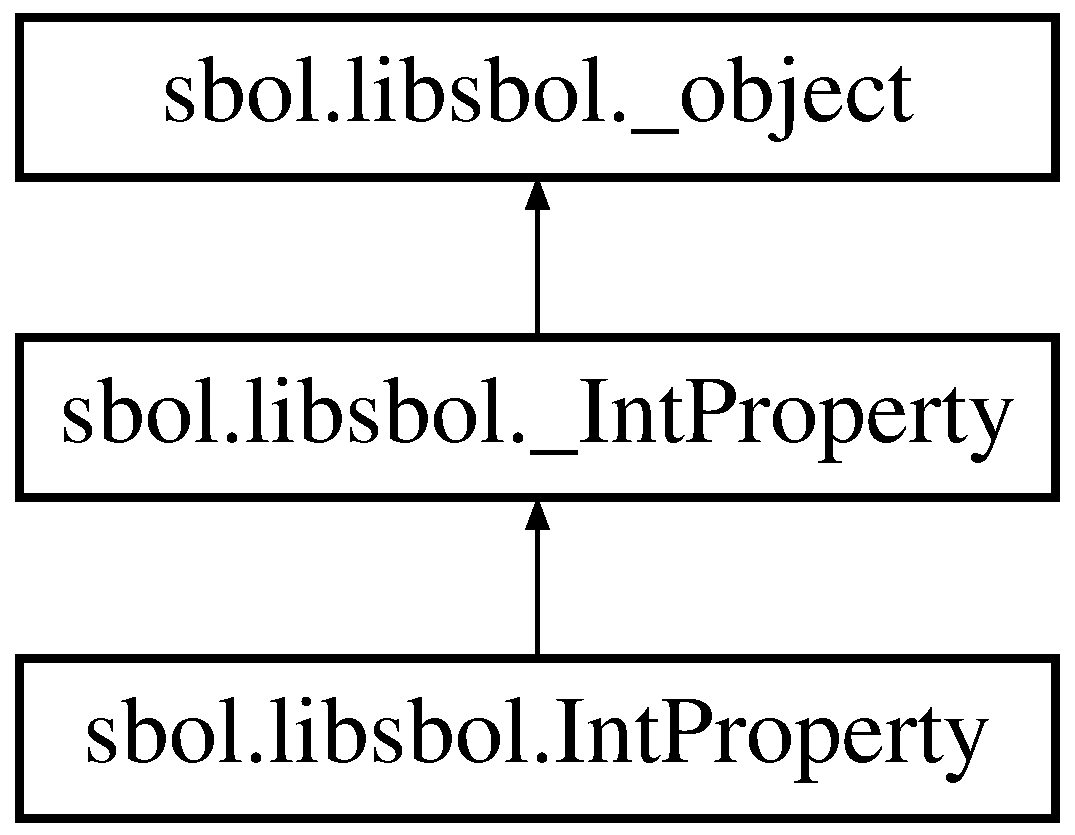
\includegraphics[height=3.000000cm]{classsbol_1_1libsbol_1_1___int_property}
\end{center}
\end{figure}
\subsection*{Public Member Functions}
\begin{DoxyCompactItemize}
\item 
def \hyperlink{classsbol_1_1libsbol_1_1___int_property_a447770d2662c639f256625bc89cd283f}{\+\_\+\+\_\+init\+\_\+\+\_\+} (self, args)
\item 
def \hyperlink{classsbol_1_1libsbol_1_1___int_property_a79c0c4757d6089b147fec27f1278a0d6}{get\+Type\+U\+RI} (self)
\item 
def \hyperlink{classsbol_1_1libsbol_1_1___int_property_af756c4fa45b885469eff547130f18f0f}{get\+Owner} (self)
\item 
def \hyperlink{classsbol_1_1libsbol_1_1___int_property_aa5baf9a8269425796be670c7b67c8895}{get} (self)
\item 
def \hyperlink{classsbol_1_1libsbol_1_1___int_property_a4bb9349161a55c81b3c9cf223f675359}{add} (self, new\+\_\+value)
\item 
def \hyperlink{classsbol_1_1libsbol_1_1___int_property_aa4fd1e97443ade53840caf3911f9e07c}{set} (self, args)
\item 
def \hyperlink{classsbol_1_1libsbol_1_1___int_property_a60af3a74ae12c94b507035f27c3ee8af}{write} (self)
\item 
def \hyperlink{classsbol_1_1libsbol_1_1___int_property_a2c806b6d53eb13817ebc2c505e6d132b}{validate} (self, arg=None)
\item 
def {\bfseries \+\_\+\+\_\+getitem\+\_\+\+\_\+} (self, n\+Index)\hypertarget{classsbol_1_1libsbol_1_1___int_property_a8657d0f89e59795177e4e5cc4e60f588}{}\label{classsbol_1_1libsbol_1_1___int_property_a8657d0f89e59795177e4e5cc4e60f588}

\item 
def {\bfseries \+\_\+\+\_\+iter\+\_\+\+\_\+} (self)\hypertarget{classsbol_1_1libsbol_1_1___int_property_a902d191c34d34911aa75b8a641a30389}{}\label{classsbol_1_1libsbol_1_1___int_property_a902d191c34d34911aa75b8a641a30389}

\item 
def {\bfseries next} (self)\hypertarget{classsbol_1_1libsbol_1_1___int_property_ab8b308262f200718831190e5ec5d0ded}{}\label{classsbol_1_1libsbol_1_1___int_property_ab8b308262f200718831190e5ec5d0ded}

\item 
def {\bfseries \+\_\+\+\_\+len\+\_\+\+\_\+} (self)\hypertarget{classsbol_1_1libsbol_1_1___int_property_ab958c6779a6640ef4f413f3fe977676e}{}\label{classsbol_1_1libsbol_1_1___int_property_ab958c6779a6640ef4f413f3fe977676e}

\end{DoxyCompactItemize}
\subsection*{Public Attributes}
\begin{DoxyCompactItemize}
\item 
{\bfseries this}\hypertarget{classsbol_1_1libsbol_1_1___int_property_a048cad663bff5e5109943ffc09b5ae38}{}\label{classsbol_1_1libsbol_1_1___int_property_a048cad663bff5e5109943ffc09b5ae38}

\end{DoxyCompactItemize}


\subsection{Detailed Description}
\begin{DoxyVerb}metafunction for generation of a map of message types to their
associated callbacks.

Usage: Use generate_callback_map<Type>::type to ...

Parameters:
-----------

LiteralType:  The library currently supports Property<string> and
Property<int> specification currently supports integer, string, and
URI literals

C++ includes: property.h 
\end{DoxyVerb}
 

\subsection{Constructor \& Destructor Documentation}
\index{sbol\+::libsbol\+::\+\_\+\+Int\+Property@{sbol\+::libsbol\+::\+\_\+\+Int\+Property}!\+\_\+\+\_\+init\+\_\+\+\_\+@{\+\_\+\+\_\+init\+\_\+\+\_\+}}
\index{\+\_\+\+\_\+init\+\_\+\+\_\+@{\+\_\+\+\_\+init\+\_\+\+\_\+}!sbol\+::libsbol\+::\+\_\+\+Int\+Property@{sbol\+::libsbol\+::\+\_\+\+Int\+Property}}
\subsubsection[{\texorpdfstring{\+\_\+\+\_\+init\+\_\+\+\_\+(self, args)}{__init__(self, args)}}]{\setlength{\rightskip}{0pt plus 5cm}def sbol.\+libsbol.\+\_\+\+Int\+Property.\+\_\+\+\_\+init\+\_\+\+\_\+ (
\begin{DoxyParamCaption}
\item[{}]{self, }
\item[{}]{args}
\end{DoxyParamCaption}
)}\hypertarget{classsbol_1_1libsbol_1_1___int_property_a447770d2662c639f256625bc89cd283f}{}\label{classsbol_1_1libsbol_1_1___int_property_a447770d2662c639f256625bc89cd283f}
\begin{DoxyVerb}sbol::Property<
LiteralType >::Property(sbol_type type_uri=UNDEFINED, void
*property_owner=NULL, ValidationRules validation_rules={}) 
\end{DoxyVerb}
 

\subsection{Member Function Documentation}
\index{sbol\+::libsbol\+::\+\_\+\+Int\+Property@{sbol\+::libsbol\+::\+\_\+\+Int\+Property}!add@{add}}
\index{add@{add}!sbol\+::libsbol\+::\+\_\+\+Int\+Property@{sbol\+::libsbol\+::\+\_\+\+Int\+Property}}
\subsubsection[{\texorpdfstring{add(self, new\+\_\+value)}{add(self, new_value)}}]{\setlength{\rightskip}{0pt plus 5cm}def sbol.\+libsbol.\+\_\+\+Int\+Property.\+add (
\begin{DoxyParamCaption}
\item[{}]{self, }
\item[{}]{new\+\_\+value}
\end{DoxyParamCaption}
)}\hypertarget{classsbol_1_1libsbol_1_1___int_property_a4bb9349161a55c81b3c9cf223f675359}{}\label{classsbol_1_1libsbol_1_1___int_property_a4bb9349161a55c81b3c9cf223f675359}
\begin{DoxyVerb}void sbol::Property<
LiteralType >::add(std::string new_value) 
\end{DoxyVerb}
 \index{sbol\+::libsbol\+::\+\_\+\+Int\+Property@{sbol\+::libsbol\+::\+\_\+\+Int\+Property}!get@{get}}
\index{get@{get}!sbol\+::libsbol\+::\+\_\+\+Int\+Property@{sbol\+::libsbol\+::\+\_\+\+Int\+Property}}
\subsubsection[{\texorpdfstring{get(self)}{get(self)}}]{\setlength{\rightskip}{0pt plus 5cm}def sbol.\+libsbol.\+\_\+\+Int\+Property.\+get (
\begin{DoxyParamCaption}
\item[{}]{self}
\end{DoxyParamCaption}
)}\hypertarget{classsbol_1_1libsbol_1_1___int_property_aa5baf9a8269425796be670c7b67c8895}{}\label{classsbol_1_1libsbol_1_1___int_property_aa5baf9a8269425796be670c7b67c8895}
\begin{DoxyVerb}std::string
sbol::Property< LiteralType >::get() 
\end{DoxyVerb}
 \index{sbol\+::libsbol\+::\+\_\+\+Int\+Property@{sbol\+::libsbol\+::\+\_\+\+Int\+Property}!get\+Owner@{get\+Owner}}
\index{get\+Owner@{get\+Owner}!sbol\+::libsbol\+::\+\_\+\+Int\+Property@{sbol\+::libsbol\+::\+\_\+\+Int\+Property}}
\subsubsection[{\texorpdfstring{get\+Owner(self)}{getOwner(self)}}]{\setlength{\rightskip}{0pt plus 5cm}def sbol.\+libsbol.\+\_\+\+Int\+Property.\+get\+Owner (
\begin{DoxyParamCaption}
\item[{}]{self}
\end{DoxyParamCaption}
)}\hypertarget{classsbol_1_1libsbol_1_1___int_property_af756c4fa45b885469eff547130f18f0f}{}\label{classsbol_1_1libsbol_1_1___int_property_af756c4fa45b885469eff547130f18f0f}
\begin{DoxyVerb}SBOLObject &
sbol::Property< LiteralType >::getOwner() 
\end{DoxyVerb}
 \index{sbol\+::libsbol\+::\+\_\+\+Int\+Property@{sbol\+::libsbol\+::\+\_\+\+Int\+Property}!get\+Type\+U\+RI@{get\+Type\+U\+RI}}
\index{get\+Type\+U\+RI@{get\+Type\+U\+RI}!sbol\+::libsbol\+::\+\_\+\+Int\+Property@{sbol\+::libsbol\+::\+\_\+\+Int\+Property}}
\subsubsection[{\texorpdfstring{get\+Type\+U\+R\+I(self)}{getTypeURI(self)}}]{\setlength{\rightskip}{0pt plus 5cm}def sbol.\+libsbol.\+\_\+\+Int\+Property.\+get\+Type\+U\+RI (
\begin{DoxyParamCaption}
\item[{}]{self}
\end{DoxyParamCaption}
)}\hypertarget{classsbol_1_1libsbol_1_1___int_property_a79c0c4757d6089b147fec27f1278a0d6}{}\label{classsbol_1_1libsbol_1_1___int_property_a79c0c4757d6089b147fec27f1278a0d6}
\begin{DoxyVerb}sbol_type
sbol::Property< LiteralType >::getTypeURI() 
\end{DoxyVerb}
 \index{sbol\+::libsbol\+::\+\_\+\+Int\+Property@{sbol\+::libsbol\+::\+\_\+\+Int\+Property}!set@{set}}
\index{set@{set}!sbol\+::libsbol\+::\+\_\+\+Int\+Property@{sbol\+::libsbol\+::\+\_\+\+Int\+Property}}
\subsubsection[{\texorpdfstring{set(self, args)}{set(self, args)}}]{\setlength{\rightskip}{0pt plus 5cm}def sbol.\+libsbol.\+\_\+\+Int\+Property.\+set (
\begin{DoxyParamCaption}
\item[{}]{self, }
\item[{}]{args}
\end{DoxyParamCaption}
)}\hypertarget{classsbol_1_1libsbol_1_1___int_property_aa4fd1e97443ade53840caf3911f9e07c}{}\label{classsbol_1_1libsbol_1_1___int_property_aa4fd1e97443ade53840caf3911f9e07c}
\begin{DoxyVerb}void sbol::Property<
LiteralType >::set(int new_value) 
\end{DoxyVerb}
 \index{sbol\+::libsbol\+::\+\_\+\+Int\+Property@{sbol\+::libsbol\+::\+\_\+\+Int\+Property}!validate@{validate}}
\index{validate@{validate}!sbol\+::libsbol\+::\+\_\+\+Int\+Property@{sbol\+::libsbol\+::\+\_\+\+Int\+Property}}
\subsubsection[{\texorpdfstring{validate(self, arg=\+None)}{validate(self, arg=None)}}]{\setlength{\rightskip}{0pt plus 5cm}def sbol.\+libsbol.\+\_\+\+Int\+Property.\+validate (
\begin{DoxyParamCaption}
\item[{}]{self, }
\item[{}]{arg = {\ttfamily None}}
\end{DoxyParamCaption}
)}\hypertarget{classsbol_1_1libsbol_1_1___int_property_a2c806b6d53eb13817ebc2c505e6d132b}{}\label{classsbol_1_1libsbol_1_1___int_property_a2c806b6d53eb13817ebc2c505e6d132b}
\begin{DoxyVerb}void sbol::Property<
LiteralType >::validate(void *arg=NULL) 
\end{DoxyVerb}
 \index{sbol\+::libsbol\+::\+\_\+\+Int\+Property@{sbol\+::libsbol\+::\+\_\+\+Int\+Property}!write@{write}}
\index{write@{write}!sbol\+::libsbol\+::\+\_\+\+Int\+Property@{sbol\+::libsbol\+::\+\_\+\+Int\+Property}}
\subsubsection[{\texorpdfstring{write(self)}{write(self)}}]{\setlength{\rightskip}{0pt plus 5cm}def sbol.\+libsbol.\+\_\+\+Int\+Property.\+write (
\begin{DoxyParamCaption}
\item[{}]{self}
\end{DoxyParamCaption}
)}\hypertarget{classsbol_1_1libsbol_1_1___int_property_a60af3a74ae12c94b507035f27c3ee8af}{}\label{classsbol_1_1libsbol_1_1___int_property_a60af3a74ae12c94b507035f27c3ee8af}
\begin{DoxyVerb}void sbol::Property<
LiteralType >::write() 
\end{DoxyVerb}
 

The documentation for this class was generated from the following file\+:\begin{DoxyCompactItemize}
\item 
libsbol.\+py\end{DoxyCompactItemize}

\hypertarget{classsbol_1_1libsbol_1_1___int_vector}{}\section{sbol.\+libsbol.\+\_\+\+Int\+Vector Class Reference}
\label{classsbol_1_1libsbol_1_1___int_vector}\index{sbol.\+libsbol.\+\_\+\+Int\+Vector@{sbol.\+libsbol.\+\_\+\+Int\+Vector}}
Inheritance diagram for sbol.\+libsbol.\+\_\+\+Int\+Vector\+:\begin{figure}[H]
\begin{center}
\leavevmode
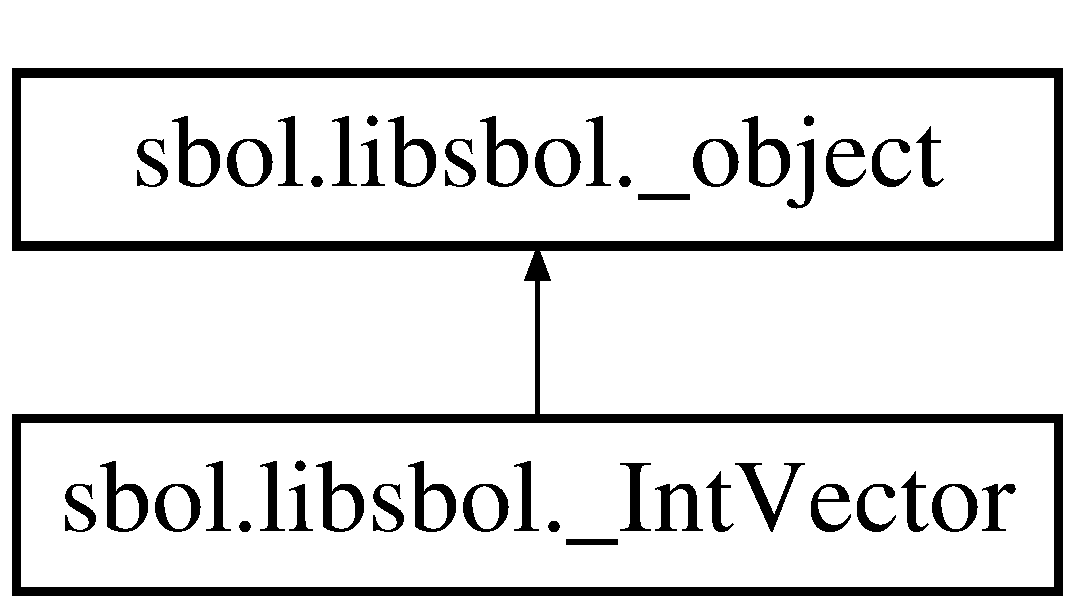
\includegraphics[height=2.000000cm]{classsbol_1_1libsbol_1_1___int_vector}
\end{center}
\end{figure}
\subsection*{Public Member Functions}
\begin{DoxyCompactItemize}
\item 
def {\bfseries iterator} (self)\hypertarget{classsbol_1_1libsbol_1_1___int_vector_a30ba1f101f39548911d393c56f869320}{}\label{classsbol_1_1libsbol_1_1___int_vector_a30ba1f101f39548911d393c56f869320}

\item 
def {\bfseries \+\_\+\+\_\+iter\+\_\+\+\_\+} (self)\hypertarget{classsbol_1_1libsbol_1_1___int_vector_aab14531083d7636c7370abbb9e292fbb}{}\label{classsbol_1_1libsbol_1_1___int_vector_aab14531083d7636c7370abbb9e292fbb}

\item 
def {\bfseries \+\_\+\+\_\+nonzero\+\_\+\+\_\+} (self)\hypertarget{classsbol_1_1libsbol_1_1___int_vector_a616908f8b3c57809b8eecef287cf246c}{}\label{classsbol_1_1libsbol_1_1___int_vector_a616908f8b3c57809b8eecef287cf246c}

\item 
def {\bfseries \+\_\+\+\_\+bool\+\_\+\+\_\+} (self)\hypertarget{classsbol_1_1libsbol_1_1___int_vector_af38a7af3dabbed3f4ad48c8e692c1a34}{}\label{classsbol_1_1libsbol_1_1___int_vector_af38a7af3dabbed3f4ad48c8e692c1a34}

\item 
def {\bfseries \+\_\+\+\_\+len\+\_\+\+\_\+} (self)\hypertarget{classsbol_1_1libsbol_1_1___int_vector_aea3cb512e66709faa42edf9e63d38128}{}\label{classsbol_1_1libsbol_1_1___int_vector_aea3cb512e66709faa42edf9e63d38128}

\item 
def {\bfseries \+\_\+\+\_\+getslice\+\_\+\+\_\+} (self, i, j)\hypertarget{classsbol_1_1libsbol_1_1___int_vector_ae872dc71848917a7fc3fd50cc421cddf}{}\label{classsbol_1_1libsbol_1_1___int_vector_ae872dc71848917a7fc3fd50cc421cddf}

\item 
def {\bfseries \+\_\+\+\_\+setslice\+\_\+\+\_\+} (self, args)\hypertarget{classsbol_1_1libsbol_1_1___int_vector_afcaa46750316e12419521393fbf49e2a}{}\label{classsbol_1_1libsbol_1_1___int_vector_afcaa46750316e12419521393fbf49e2a}

\item 
def {\bfseries \+\_\+\+\_\+delslice\+\_\+\+\_\+} (self, i, j)\hypertarget{classsbol_1_1libsbol_1_1___int_vector_a0ae6d5fa2290ff5f00c0f153b3165f39}{}\label{classsbol_1_1libsbol_1_1___int_vector_a0ae6d5fa2290ff5f00c0f153b3165f39}

\item 
def {\bfseries \+\_\+\+\_\+delitem\+\_\+\+\_\+} (self, args)\hypertarget{classsbol_1_1libsbol_1_1___int_vector_a999400f4728878ab77a3995dcfe50125}{}\label{classsbol_1_1libsbol_1_1___int_vector_a999400f4728878ab77a3995dcfe50125}

\item 
def {\bfseries \+\_\+\+\_\+getitem\+\_\+\+\_\+} (self, args)\hypertarget{classsbol_1_1libsbol_1_1___int_vector_a524082d914e028d96cc30a4943c6acf6}{}\label{classsbol_1_1libsbol_1_1___int_vector_a524082d914e028d96cc30a4943c6acf6}

\item 
def {\bfseries \+\_\+\+\_\+setitem\+\_\+\+\_\+} (self, args)\hypertarget{classsbol_1_1libsbol_1_1___int_vector_abe5317ccb4b26ae9f72025e27611cbce}{}\label{classsbol_1_1libsbol_1_1___int_vector_abe5317ccb4b26ae9f72025e27611cbce}

\item 
def {\bfseries pop} (self)\hypertarget{classsbol_1_1libsbol_1_1___int_vector_ae9ddc6bd9167fb12c27bcc50d9e0997e}{}\label{classsbol_1_1libsbol_1_1___int_vector_ae9ddc6bd9167fb12c27bcc50d9e0997e}

\item 
def {\bfseries append} (self, x)\hypertarget{classsbol_1_1libsbol_1_1___int_vector_ab0061a8eba628a029df78fbaad964f44}{}\label{classsbol_1_1libsbol_1_1___int_vector_ab0061a8eba628a029df78fbaad964f44}

\item 
def {\bfseries empty} (self)\hypertarget{classsbol_1_1libsbol_1_1___int_vector_a319a638fe90cc649a4d13b4b78b120f0}{}\label{classsbol_1_1libsbol_1_1___int_vector_a319a638fe90cc649a4d13b4b78b120f0}

\item 
def {\bfseries size} (self)\hypertarget{classsbol_1_1libsbol_1_1___int_vector_a82a8efd708baeb0801f29c544960af53}{}\label{classsbol_1_1libsbol_1_1___int_vector_a82a8efd708baeb0801f29c544960af53}

\item 
def {\bfseries swap} (self, v)\hypertarget{classsbol_1_1libsbol_1_1___int_vector_a8c808697f5b2c971aa2780d86f8d6993}{}\label{classsbol_1_1libsbol_1_1___int_vector_a8c808697f5b2c971aa2780d86f8d6993}

\item 
def {\bfseries begin} (self)\hypertarget{classsbol_1_1libsbol_1_1___int_vector_a3737c8e83c110ceece6fe47dc8f906cc}{}\label{classsbol_1_1libsbol_1_1___int_vector_a3737c8e83c110ceece6fe47dc8f906cc}

\item 
def {\bfseries end} (self)\hypertarget{classsbol_1_1libsbol_1_1___int_vector_a42ec52eb0bc1344f84810a12908e1272}{}\label{classsbol_1_1libsbol_1_1___int_vector_a42ec52eb0bc1344f84810a12908e1272}

\item 
def {\bfseries rbegin} (self)\hypertarget{classsbol_1_1libsbol_1_1___int_vector_a749694f66d884c9f49cec0325d5b5d35}{}\label{classsbol_1_1libsbol_1_1___int_vector_a749694f66d884c9f49cec0325d5b5d35}

\item 
def {\bfseries rend} (self)\hypertarget{classsbol_1_1libsbol_1_1___int_vector_aec1824d8372546a3876125bc3ae34742}{}\label{classsbol_1_1libsbol_1_1___int_vector_aec1824d8372546a3876125bc3ae34742}

\item 
def {\bfseries clear} (self)\hypertarget{classsbol_1_1libsbol_1_1___int_vector_a03cba1917e3257ac402877254667cc17}{}\label{classsbol_1_1libsbol_1_1___int_vector_a03cba1917e3257ac402877254667cc17}

\item 
def {\bfseries get\+\_\+allocator} (self)\hypertarget{classsbol_1_1libsbol_1_1___int_vector_a916113cf9341759ef68cf372a575bd46}{}\label{classsbol_1_1libsbol_1_1___int_vector_a916113cf9341759ef68cf372a575bd46}

\item 
def {\bfseries pop\+\_\+back} (self)\hypertarget{classsbol_1_1libsbol_1_1___int_vector_abac576e0546053bae199b3ad0bad9b5e}{}\label{classsbol_1_1libsbol_1_1___int_vector_abac576e0546053bae199b3ad0bad9b5e}

\item 
def {\bfseries erase} (self, args)\hypertarget{classsbol_1_1libsbol_1_1___int_vector_ab424433b043b22fbb87eb9e7ee541037}{}\label{classsbol_1_1libsbol_1_1___int_vector_ab424433b043b22fbb87eb9e7ee541037}

\item 
def {\bfseries \+\_\+\+\_\+init\+\_\+\+\_\+} (self, args)\hypertarget{classsbol_1_1libsbol_1_1___int_vector_a4f4ec35fa2199094c7494a291cf42740}{}\label{classsbol_1_1libsbol_1_1___int_vector_a4f4ec35fa2199094c7494a291cf42740}

\item 
def {\bfseries push\+\_\+back} (self, x)\hypertarget{classsbol_1_1libsbol_1_1___int_vector_ad0841fc19c70755e29eac3e13241cb54}{}\label{classsbol_1_1libsbol_1_1___int_vector_ad0841fc19c70755e29eac3e13241cb54}

\item 
def {\bfseries front} (self)\hypertarget{classsbol_1_1libsbol_1_1___int_vector_a8078087f51b5356758ff925c86db5526}{}\label{classsbol_1_1libsbol_1_1___int_vector_a8078087f51b5356758ff925c86db5526}

\item 
def {\bfseries back} (self)\hypertarget{classsbol_1_1libsbol_1_1___int_vector_afcddc4d2b7e8630fd963b051af25603f}{}\label{classsbol_1_1libsbol_1_1___int_vector_afcddc4d2b7e8630fd963b051af25603f}

\item 
def {\bfseries assign} (self, n, x)\hypertarget{classsbol_1_1libsbol_1_1___int_vector_ac09e4a34f9b9f9b67d08e82a00050a5c}{}\label{classsbol_1_1libsbol_1_1___int_vector_ac09e4a34f9b9f9b67d08e82a00050a5c}

\item 
def {\bfseries resize} (self, args)\hypertarget{classsbol_1_1libsbol_1_1___int_vector_a799d8ddc6e4b1fd16bcb1c9f1c97a81b}{}\label{classsbol_1_1libsbol_1_1___int_vector_a799d8ddc6e4b1fd16bcb1c9f1c97a81b}

\item 
def {\bfseries insert} (self, args)\hypertarget{classsbol_1_1libsbol_1_1___int_vector_a536678fe48e99152750e1cd24094a536}{}\label{classsbol_1_1libsbol_1_1___int_vector_a536678fe48e99152750e1cd24094a536}

\item 
def {\bfseries reserve} (self, n)\hypertarget{classsbol_1_1libsbol_1_1___int_vector_a91769189eb0cdb030883bc4042ff3c80}{}\label{classsbol_1_1libsbol_1_1___int_vector_a91769189eb0cdb030883bc4042ff3c80}

\item 
def {\bfseries capacity} (self)\hypertarget{classsbol_1_1libsbol_1_1___int_vector_ad3e4e9e9de5255a7742baebee6aa9f71}{}\label{classsbol_1_1libsbol_1_1___int_vector_ad3e4e9e9de5255a7742baebee6aa9f71}

\end{DoxyCompactItemize}
\subsection*{Public Attributes}
\begin{DoxyCompactItemize}
\item 
{\bfseries this}\hypertarget{classsbol_1_1libsbol_1_1___int_vector_a27634641f0321b8932802d3187918c82}{}\label{classsbol_1_1libsbol_1_1___int_vector_a27634641f0321b8932802d3187918c82}

\end{DoxyCompactItemize}


The documentation for this class was generated from the following file\+:\begin{DoxyCompactItemize}
\item 
libsbol.\+py\end{DoxyCompactItemize}

\hypertarget{classsbol_1_1libsbol_1_1___map_of_s_b_o_l_object}{}\section{sbol.\+libsbol.\+\_\+\+Map\+Of\+S\+B\+O\+L\+Object Class Reference}
\label{classsbol_1_1libsbol_1_1___map_of_s_b_o_l_object}\index{sbol.\+libsbol.\+\_\+\+Map\+Of\+S\+B\+O\+L\+Object@{sbol.\+libsbol.\+\_\+\+Map\+Of\+S\+B\+O\+L\+Object}}
Inheritance diagram for sbol.\+libsbol.\+\_\+\+Map\+Of\+S\+B\+O\+L\+Object\+:\begin{figure}[H]
\begin{center}
\leavevmode
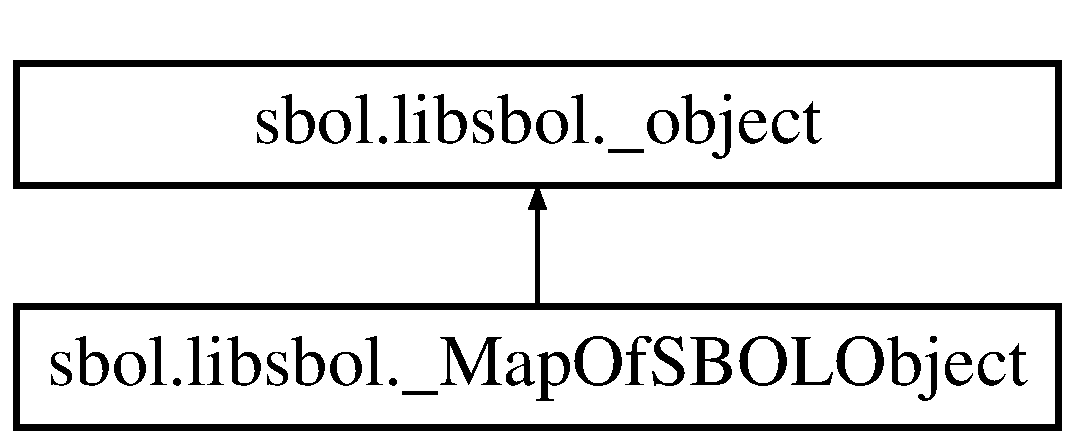
\includegraphics[height=2.000000cm]{classsbol_1_1libsbol_1_1___map_of_s_b_o_l_object}
\end{center}
\end{figure}
\subsection*{Public Member Functions}
\begin{DoxyCompactItemize}
\item 
def {\bfseries iterator} (self)\hypertarget{classsbol_1_1libsbol_1_1___map_of_s_b_o_l_object_a99896b246746e8d9f49dced6553d8123}{}\label{classsbol_1_1libsbol_1_1___map_of_s_b_o_l_object_a99896b246746e8d9f49dced6553d8123}

\item 
def {\bfseries \+\_\+\+\_\+iter\+\_\+\+\_\+} (self)\hypertarget{classsbol_1_1libsbol_1_1___map_of_s_b_o_l_object_a2ff30b1a2e8e8d038af401ed0ce6628c}{}\label{classsbol_1_1libsbol_1_1___map_of_s_b_o_l_object_a2ff30b1a2e8e8d038af401ed0ce6628c}

\item 
def {\bfseries \+\_\+\+\_\+nonzero\+\_\+\+\_\+} (self)\hypertarget{classsbol_1_1libsbol_1_1___map_of_s_b_o_l_object_a89468c6b07067b8a3d18677696f5013a}{}\label{classsbol_1_1libsbol_1_1___map_of_s_b_o_l_object_a89468c6b07067b8a3d18677696f5013a}

\item 
def {\bfseries \+\_\+\+\_\+bool\+\_\+\+\_\+} (self)\hypertarget{classsbol_1_1libsbol_1_1___map_of_s_b_o_l_object_a4ee74e7a7de817c51cc5d0b94441f8f7}{}\label{classsbol_1_1libsbol_1_1___map_of_s_b_o_l_object_a4ee74e7a7de817c51cc5d0b94441f8f7}

\item 
def {\bfseries \+\_\+\+\_\+len\+\_\+\+\_\+} (self)\hypertarget{classsbol_1_1libsbol_1_1___map_of_s_b_o_l_object_a5f244a1c1cbd30de43df6b2d8667f04b}{}\label{classsbol_1_1libsbol_1_1___map_of_s_b_o_l_object_a5f244a1c1cbd30de43df6b2d8667f04b}

\item 
def {\bfseries \+\_\+\+\_\+iter\+\_\+\+\_\+} (self)\hypertarget{classsbol_1_1libsbol_1_1___map_of_s_b_o_l_object_a2ff30b1a2e8e8d038af401ed0ce6628c}{}\label{classsbol_1_1libsbol_1_1___map_of_s_b_o_l_object_a2ff30b1a2e8e8d038af401ed0ce6628c}

\item 
def {\bfseries iterkeys} (self)\hypertarget{classsbol_1_1libsbol_1_1___map_of_s_b_o_l_object_abebe007101a1bae6e10e49f135d31734}{}\label{classsbol_1_1libsbol_1_1___map_of_s_b_o_l_object_abebe007101a1bae6e10e49f135d31734}

\item 
def {\bfseries itervalues} (self)\hypertarget{classsbol_1_1libsbol_1_1___map_of_s_b_o_l_object_ad751a3d8ea3be789fdb0d5f2f86ce4a0}{}\label{classsbol_1_1libsbol_1_1___map_of_s_b_o_l_object_ad751a3d8ea3be789fdb0d5f2f86ce4a0}

\item 
def {\bfseries iteritems} (self)\hypertarget{classsbol_1_1libsbol_1_1___map_of_s_b_o_l_object_a05361b0bf45d68c2231b975d5414daba}{}\label{classsbol_1_1libsbol_1_1___map_of_s_b_o_l_object_a05361b0bf45d68c2231b975d5414daba}

\item 
def {\bfseries \+\_\+\+\_\+getitem\+\_\+\+\_\+} (self, key)\hypertarget{classsbol_1_1libsbol_1_1___map_of_s_b_o_l_object_a3b22c8d628956f07a515bd7cf3996bf7}{}\label{classsbol_1_1libsbol_1_1___map_of_s_b_o_l_object_a3b22c8d628956f07a515bd7cf3996bf7}

\item 
def {\bfseries \+\_\+\+\_\+delitem\+\_\+\+\_\+} (self, key)\hypertarget{classsbol_1_1libsbol_1_1___map_of_s_b_o_l_object_ac562870c0d173a5a5bc7799929341be5}{}\label{classsbol_1_1libsbol_1_1___map_of_s_b_o_l_object_ac562870c0d173a5a5bc7799929341be5}

\item 
def {\bfseries has\+\_\+key} (self, key)\hypertarget{classsbol_1_1libsbol_1_1___map_of_s_b_o_l_object_a0b1d6d592453e758aaa8eeda07ea224f}{}\label{classsbol_1_1libsbol_1_1___map_of_s_b_o_l_object_a0b1d6d592453e758aaa8eeda07ea224f}

\item 
def {\bfseries keys} (self)\hypertarget{classsbol_1_1libsbol_1_1___map_of_s_b_o_l_object_aae3e52f12cdc1d7c91441a2ab8d41a9d}{}\label{classsbol_1_1libsbol_1_1___map_of_s_b_o_l_object_aae3e52f12cdc1d7c91441a2ab8d41a9d}

\item 
def {\bfseries values} (self)\hypertarget{classsbol_1_1libsbol_1_1___map_of_s_b_o_l_object_a70d9ef173a69e7d4184dbb0d64488870}{}\label{classsbol_1_1libsbol_1_1___map_of_s_b_o_l_object_a70d9ef173a69e7d4184dbb0d64488870}

\item 
def {\bfseries items} (self)\hypertarget{classsbol_1_1libsbol_1_1___map_of_s_b_o_l_object_a495e0f2c09340ed303e43fd19ee1673f}{}\label{classsbol_1_1libsbol_1_1___map_of_s_b_o_l_object_a495e0f2c09340ed303e43fd19ee1673f}

\item 
def {\bfseries \+\_\+\+\_\+contains\+\_\+\+\_\+} (self, key)\hypertarget{classsbol_1_1libsbol_1_1___map_of_s_b_o_l_object_abdfe1e05e80c80590a564e6e4b6d54b2}{}\label{classsbol_1_1libsbol_1_1___map_of_s_b_o_l_object_abdfe1e05e80c80590a564e6e4b6d54b2}

\item 
def {\bfseries key\+\_\+iterator} (self)\hypertarget{classsbol_1_1libsbol_1_1___map_of_s_b_o_l_object_ab8c0c90697fb2b10e3e56d8fc94a755c}{}\label{classsbol_1_1libsbol_1_1___map_of_s_b_o_l_object_ab8c0c90697fb2b10e3e56d8fc94a755c}

\item 
def {\bfseries value\+\_\+iterator} (self)\hypertarget{classsbol_1_1libsbol_1_1___map_of_s_b_o_l_object_a80904ae351e4260a765c1d793b69c8e1}{}\label{classsbol_1_1libsbol_1_1___map_of_s_b_o_l_object_a80904ae351e4260a765c1d793b69c8e1}

\item 
def {\bfseries \+\_\+\+\_\+setitem\+\_\+\+\_\+} (self, args)\hypertarget{classsbol_1_1libsbol_1_1___map_of_s_b_o_l_object_a1f6df57e89b24ed785d1ec0021d22586}{}\label{classsbol_1_1libsbol_1_1___map_of_s_b_o_l_object_a1f6df57e89b24ed785d1ec0021d22586}

\item 
def {\bfseries asdict} (self)\hypertarget{classsbol_1_1libsbol_1_1___map_of_s_b_o_l_object_a8aec1726119d4fa08d653f03ff4549f5}{}\label{classsbol_1_1libsbol_1_1___map_of_s_b_o_l_object_a8aec1726119d4fa08d653f03ff4549f5}

\item 
def {\bfseries \+\_\+\+\_\+init\+\_\+\+\_\+} (self, args)\hypertarget{classsbol_1_1libsbol_1_1___map_of_s_b_o_l_object_add0cfd1fd6d6841fbe58a2178f8068a5}{}\label{classsbol_1_1libsbol_1_1___map_of_s_b_o_l_object_add0cfd1fd6d6841fbe58a2178f8068a5}

\item 
def {\bfseries empty} (self)\hypertarget{classsbol_1_1libsbol_1_1___map_of_s_b_o_l_object_acd2c979d7914170ac9ce6e4c5a897559}{}\label{classsbol_1_1libsbol_1_1___map_of_s_b_o_l_object_acd2c979d7914170ac9ce6e4c5a897559}

\item 
def {\bfseries size} (self)\hypertarget{classsbol_1_1libsbol_1_1___map_of_s_b_o_l_object_ae6c8f4c1286099afa21a3a4bc554cc50}{}\label{classsbol_1_1libsbol_1_1___map_of_s_b_o_l_object_ae6c8f4c1286099afa21a3a4bc554cc50}

\item 
def {\bfseries swap} (self, v)\hypertarget{classsbol_1_1libsbol_1_1___map_of_s_b_o_l_object_a17ae1c7230e9bac22b0a636731ccb644}{}\label{classsbol_1_1libsbol_1_1___map_of_s_b_o_l_object_a17ae1c7230e9bac22b0a636731ccb644}

\item 
def {\bfseries begin} (self)\hypertarget{classsbol_1_1libsbol_1_1___map_of_s_b_o_l_object_ac7583d492529ca5c3a648220d2f3f11d}{}\label{classsbol_1_1libsbol_1_1___map_of_s_b_o_l_object_ac7583d492529ca5c3a648220d2f3f11d}

\item 
def {\bfseries end} (self)\hypertarget{classsbol_1_1libsbol_1_1___map_of_s_b_o_l_object_ab076559dfeeec29110aa14234e2da96f}{}\label{classsbol_1_1libsbol_1_1___map_of_s_b_o_l_object_ab076559dfeeec29110aa14234e2da96f}

\item 
def {\bfseries rbegin} (self)\hypertarget{classsbol_1_1libsbol_1_1___map_of_s_b_o_l_object_acf70e03c15a8aa7c3bda9b6cf0e3db7c}{}\label{classsbol_1_1libsbol_1_1___map_of_s_b_o_l_object_acf70e03c15a8aa7c3bda9b6cf0e3db7c}

\item 
def {\bfseries rend} (self)\hypertarget{classsbol_1_1libsbol_1_1___map_of_s_b_o_l_object_a285867409ce0c637fa34245520a9f44b}{}\label{classsbol_1_1libsbol_1_1___map_of_s_b_o_l_object_a285867409ce0c637fa34245520a9f44b}

\item 
def {\bfseries clear} (self)\hypertarget{classsbol_1_1libsbol_1_1___map_of_s_b_o_l_object_a85655f14478d8da325e30156643fed2f}{}\label{classsbol_1_1libsbol_1_1___map_of_s_b_o_l_object_a85655f14478d8da325e30156643fed2f}

\item 
def {\bfseries get\+\_\+allocator} (self)\hypertarget{classsbol_1_1libsbol_1_1___map_of_s_b_o_l_object_adb29fc9a623c911251624af12c2e5b82}{}\label{classsbol_1_1libsbol_1_1___map_of_s_b_o_l_object_adb29fc9a623c911251624af12c2e5b82}

\item 
def {\bfseries count} (self, x)\hypertarget{classsbol_1_1libsbol_1_1___map_of_s_b_o_l_object_a711455fcad42ecd74d866cbcc7ec1df6}{}\label{classsbol_1_1libsbol_1_1___map_of_s_b_o_l_object_a711455fcad42ecd74d866cbcc7ec1df6}

\item 
def {\bfseries erase} (self, args)\hypertarget{classsbol_1_1libsbol_1_1___map_of_s_b_o_l_object_a0a6076cca589d14a787f9ee9272ac7ab}{}\label{classsbol_1_1libsbol_1_1___map_of_s_b_o_l_object_a0a6076cca589d14a787f9ee9272ac7ab}

\item 
def {\bfseries find} (self, x)\hypertarget{classsbol_1_1libsbol_1_1___map_of_s_b_o_l_object_a4828ba5e97b23331c93dba3e26475368}{}\label{classsbol_1_1libsbol_1_1___map_of_s_b_o_l_object_a4828ba5e97b23331c93dba3e26475368}

\item 
def {\bfseries lower\+\_\+bound} (self, x)\hypertarget{classsbol_1_1libsbol_1_1___map_of_s_b_o_l_object_a880b384d747348ac85bd4046c4130905}{}\label{classsbol_1_1libsbol_1_1___map_of_s_b_o_l_object_a880b384d747348ac85bd4046c4130905}

\item 
def {\bfseries upper\+\_\+bound} (self, x)\hypertarget{classsbol_1_1libsbol_1_1___map_of_s_b_o_l_object_afe2ee6b1f7a190daa9ac02ff325d8895}{}\label{classsbol_1_1libsbol_1_1___map_of_s_b_o_l_object_afe2ee6b1f7a190daa9ac02ff325d8895}

\end{DoxyCompactItemize}
\subsection*{Public Attributes}
\begin{DoxyCompactItemize}
\item 
{\bfseries this}\hypertarget{classsbol_1_1libsbol_1_1___map_of_s_b_o_l_object_a674b0b6ff103d35c8b33e4d96d3eabe0}{}\label{classsbol_1_1libsbol_1_1___map_of_s_b_o_l_object_a674b0b6ff103d35c8b33e4d96d3eabe0}

\end{DoxyCompactItemize}


The documentation for this class was generated from the following file\+:\begin{DoxyCompactItemize}
\item 
libsbol.\+py\end{DoxyCompactItemize}

\hypertarget{classsbol_1_1libsbol_1_1___map_of_string_vector}{}\section{sbol.\+libsbol.\+\_\+\+Map\+Of\+String\+Vector Class Reference}
\label{classsbol_1_1libsbol_1_1___map_of_string_vector}\index{sbol.\+libsbol.\+\_\+\+Map\+Of\+String\+Vector@{sbol.\+libsbol.\+\_\+\+Map\+Of\+String\+Vector}}
Inheritance diagram for sbol.\+libsbol.\+\_\+\+Map\+Of\+String\+Vector\+:\begin{figure}[H]
\begin{center}
\leavevmode
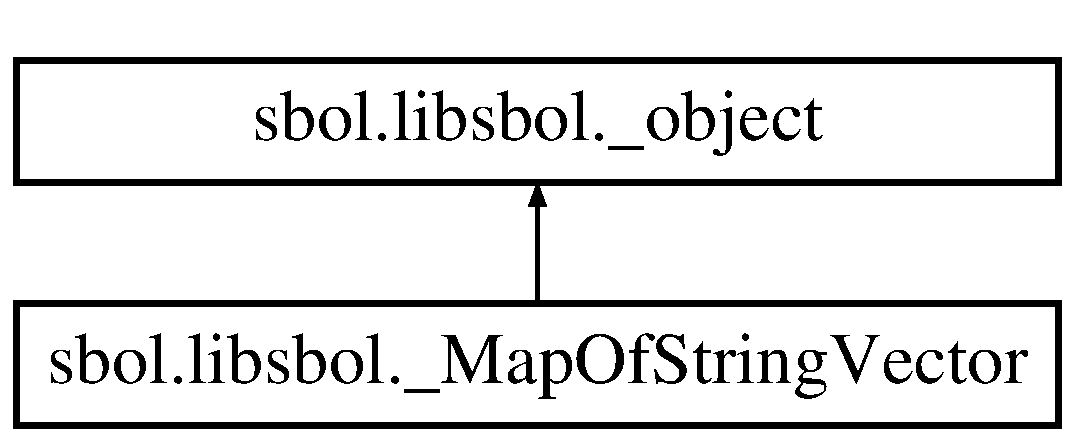
\includegraphics[height=2.000000cm]{classsbol_1_1libsbol_1_1___map_of_string_vector}
\end{center}
\end{figure}
\subsection*{Public Member Functions}
\begin{DoxyCompactItemize}
\item 
def {\bfseries iterator} (self)\hypertarget{classsbol_1_1libsbol_1_1___map_of_string_vector_a2ef365e418b7abbce2f78192d09ae70f}{}\label{classsbol_1_1libsbol_1_1___map_of_string_vector_a2ef365e418b7abbce2f78192d09ae70f}

\item 
def {\bfseries \+\_\+\+\_\+iter\+\_\+\+\_\+} (self)\hypertarget{classsbol_1_1libsbol_1_1___map_of_string_vector_a24ec9058c556d0ce97018de40f6fd2b0}{}\label{classsbol_1_1libsbol_1_1___map_of_string_vector_a24ec9058c556d0ce97018de40f6fd2b0}

\item 
def {\bfseries \+\_\+\+\_\+nonzero\+\_\+\+\_\+} (self)\hypertarget{classsbol_1_1libsbol_1_1___map_of_string_vector_a9ffcecddcf18eaf7ed5fbdc18978f6d3}{}\label{classsbol_1_1libsbol_1_1___map_of_string_vector_a9ffcecddcf18eaf7ed5fbdc18978f6d3}

\item 
def {\bfseries \+\_\+\+\_\+bool\+\_\+\+\_\+} (self)\hypertarget{classsbol_1_1libsbol_1_1___map_of_string_vector_aba744b5b2078eeecec17dbfbe76edd92}{}\label{classsbol_1_1libsbol_1_1___map_of_string_vector_aba744b5b2078eeecec17dbfbe76edd92}

\item 
def {\bfseries \+\_\+\+\_\+len\+\_\+\+\_\+} (self)\hypertarget{classsbol_1_1libsbol_1_1___map_of_string_vector_a5773bf31f5e130dce7f8bad762ae98d2}{}\label{classsbol_1_1libsbol_1_1___map_of_string_vector_a5773bf31f5e130dce7f8bad762ae98d2}

\item 
def {\bfseries \+\_\+\+\_\+iter\+\_\+\+\_\+} (self)\hypertarget{classsbol_1_1libsbol_1_1___map_of_string_vector_a24ec9058c556d0ce97018de40f6fd2b0}{}\label{classsbol_1_1libsbol_1_1___map_of_string_vector_a24ec9058c556d0ce97018de40f6fd2b0}

\item 
def {\bfseries iterkeys} (self)\hypertarget{classsbol_1_1libsbol_1_1___map_of_string_vector_a4db85a53b167cf2b1ed92af382b410eb}{}\label{classsbol_1_1libsbol_1_1___map_of_string_vector_a4db85a53b167cf2b1ed92af382b410eb}

\item 
def {\bfseries itervalues} (self)\hypertarget{classsbol_1_1libsbol_1_1___map_of_string_vector_a8ef7006738e576d150959747099951cb}{}\label{classsbol_1_1libsbol_1_1___map_of_string_vector_a8ef7006738e576d150959747099951cb}

\item 
def {\bfseries iteritems} (self)\hypertarget{classsbol_1_1libsbol_1_1___map_of_string_vector_a2b11f2a512e8c95520de8ee68362175d}{}\label{classsbol_1_1libsbol_1_1___map_of_string_vector_a2b11f2a512e8c95520de8ee68362175d}

\item 
def {\bfseries \+\_\+\+\_\+getitem\+\_\+\+\_\+} (self, key)\hypertarget{classsbol_1_1libsbol_1_1___map_of_string_vector_af194196545f480e295f651f54b456109}{}\label{classsbol_1_1libsbol_1_1___map_of_string_vector_af194196545f480e295f651f54b456109}

\item 
def {\bfseries \+\_\+\+\_\+delitem\+\_\+\+\_\+} (self, key)\hypertarget{classsbol_1_1libsbol_1_1___map_of_string_vector_ae35cea3e90d6d76a44ac5dff43ab689d}{}\label{classsbol_1_1libsbol_1_1___map_of_string_vector_ae35cea3e90d6d76a44ac5dff43ab689d}

\item 
def {\bfseries has\+\_\+key} (self, key)\hypertarget{classsbol_1_1libsbol_1_1___map_of_string_vector_adc02fdcc92ae389a8f3d65ed232809c2}{}\label{classsbol_1_1libsbol_1_1___map_of_string_vector_adc02fdcc92ae389a8f3d65ed232809c2}

\item 
def {\bfseries keys} (self)\hypertarget{classsbol_1_1libsbol_1_1___map_of_string_vector_aefaf997539c13ce75f9425da3e9b7d7e}{}\label{classsbol_1_1libsbol_1_1___map_of_string_vector_aefaf997539c13ce75f9425da3e9b7d7e}

\item 
def {\bfseries values} (self)\hypertarget{classsbol_1_1libsbol_1_1___map_of_string_vector_ab825ef9a3080e56a7cf02b3c37af11c2}{}\label{classsbol_1_1libsbol_1_1___map_of_string_vector_ab825ef9a3080e56a7cf02b3c37af11c2}

\item 
def {\bfseries items} (self)\hypertarget{classsbol_1_1libsbol_1_1___map_of_string_vector_a60031d8ad0a471836bbf914ca96696ef}{}\label{classsbol_1_1libsbol_1_1___map_of_string_vector_a60031d8ad0a471836bbf914ca96696ef}

\item 
def {\bfseries \+\_\+\+\_\+contains\+\_\+\+\_\+} (self, key)\hypertarget{classsbol_1_1libsbol_1_1___map_of_string_vector_a21f05f23abf329ecd83a62474c4f8fc6}{}\label{classsbol_1_1libsbol_1_1___map_of_string_vector_a21f05f23abf329ecd83a62474c4f8fc6}

\item 
def {\bfseries key\+\_\+iterator} (self)\hypertarget{classsbol_1_1libsbol_1_1___map_of_string_vector_ac2ffd22674b537b18e142fd03459bb13}{}\label{classsbol_1_1libsbol_1_1___map_of_string_vector_ac2ffd22674b537b18e142fd03459bb13}

\item 
def {\bfseries value\+\_\+iterator} (self)\hypertarget{classsbol_1_1libsbol_1_1___map_of_string_vector_a8ed4f452b77da98bca42f8945d953c62}{}\label{classsbol_1_1libsbol_1_1___map_of_string_vector_a8ed4f452b77da98bca42f8945d953c62}

\item 
def {\bfseries \+\_\+\+\_\+setitem\+\_\+\+\_\+} (self, args)\hypertarget{classsbol_1_1libsbol_1_1___map_of_string_vector_a03ed9077692f0534f2f16952fc18791e}{}\label{classsbol_1_1libsbol_1_1___map_of_string_vector_a03ed9077692f0534f2f16952fc18791e}

\item 
def {\bfseries asdict} (self)\hypertarget{classsbol_1_1libsbol_1_1___map_of_string_vector_aac595943ae74b2b6aa3963be32618295}{}\label{classsbol_1_1libsbol_1_1___map_of_string_vector_aac595943ae74b2b6aa3963be32618295}

\item 
def {\bfseries \+\_\+\+\_\+init\+\_\+\+\_\+} (self, args)\hypertarget{classsbol_1_1libsbol_1_1___map_of_string_vector_a8ebe8c22c35679800cf084ffa3ebf43f}{}\label{classsbol_1_1libsbol_1_1___map_of_string_vector_a8ebe8c22c35679800cf084ffa3ebf43f}

\item 
def {\bfseries empty} (self)\hypertarget{classsbol_1_1libsbol_1_1___map_of_string_vector_a861304b68ea9354efc2073a125636a85}{}\label{classsbol_1_1libsbol_1_1___map_of_string_vector_a861304b68ea9354efc2073a125636a85}

\item 
def {\bfseries size} (self)\hypertarget{classsbol_1_1libsbol_1_1___map_of_string_vector_a115426862fe18e46cf77f02793509a61}{}\label{classsbol_1_1libsbol_1_1___map_of_string_vector_a115426862fe18e46cf77f02793509a61}

\item 
def {\bfseries swap} (self, v)\hypertarget{classsbol_1_1libsbol_1_1___map_of_string_vector_acdf2263cf698b77d3cd2e643138ef39c}{}\label{classsbol_1_1libsbol_1_1___map_of_string_vector_acdf2263cf698b77d3cd2e643138ef39c}

\item 
def {\bfseries begin} (self)\hypertarget{classsbol_1_1libsbol_1_1___map_of_string_vector_a32a03987ee118d3a27cdd05d03162461}{}\label{classsbol_1_1libsbol_1_1___map_of_string_vector_a32a03987ee118d3a27cdd05d03162461}

\item 
def {\bfseries end} (self)\hypertarget{classsbol_1_1libsbol_1_1___map_of_string_vector_af4c234ac8f5357c12a5236bc351e61d9}{}\label{classsbol_1_1libsbol_1_1___map_of_string_vector_af4c234ac8f5357c12a5236bc351e61d9}

\item 
def {\bfseries rbegin} (self)\hypertarget{classsbol_1_1libsbol_1_1___map_of_string_vector_a56dbe5503409ca1e7fc1e25c84af636a}{}\label{classsbol_1_1libsbol_1_1___map_of_string_vector_a56dbe5503409ca1e7fc1e25c84af636a}

\item 
def {\bfseries rend} (self)\hypertarget{classsbol_1_1libsbol_1_1___map_of_string_vector_a7329b3147a5af8cbd753570dcf561c0b}{}\label{classsbol_1_1libsbol_1_1___map_of_string_vector_a7329b3147a5af8cbd753570dcf561c0b}

\item 
def {\bfseries clear} (self)\hypertarget{classsbol_1_1libsbol_1_1___map_of_string_vector_adb8dd18011f51e48b4681e757ef1e452}{}\label{classsbol_1_1libsbol_1_1___map_of_string_vector_adb8dd18011f51e48b4681e757ef1e452}

\item 
def {\bfseries get\+\_\+allocator} (self)\hypertarget{classsbol_1_1libsbol_1_1___map_of_string_vector_a7e455e8b2aa049ea81dc90d345358bca}{}\label{classsbol_1_1libsbol_1_1___map_of_string_vector_a7e455e8b2aa049ea81dc90d345358bca}

\item 
def {\bfseries count} (self, x)\hypertarget{classsbol_1_1libsbol_1_1___map_of_string_vector_a14f5651dffbbcaff5ac021086f336fc2}{}\label{classsbol_1_1libsbol_1_1___map_of_string_vector_a14f5651dffbbcaff5ac021086f336fc2}

\item 
def {\bfseries erase} (self, args)\hypertarget{classsbol_1_1libsbol_1_1___map_of_string_vector_a3fecad41a5dd88c86c05e4f5bdfb5570}{}\label{classsbol_1_1libsbol_1_1___map_of_string_vector_a3fecad41a5dd88c86c05e4f5bdfb5570}

\item 
def {\bfseries find} (self, x)\hypertarget{classsbol_1_1libsbol_1_1___map_of_string_vector_aef3d4285037f7d48282cb7080cadb834}{}\label{classsbol_1_1libsbol_1_1___map_of_string_vector_aef3d4285037f7d48282cb7080cadb834}

\item 
def {\bfseries lower\+\_\+bound} (self, x)\hypertarget{classsbol_1_1libsbol_1_1___map_of_string_vector_a6527de6055587be8b0ecf463cc0637df}{}\label{classsbol_1_1libsbol_1_1___map_of_string_vector_a6527de6055587be8b0ecf463cc0637df}

\item 
def {\bfseries upper\+\_\+bound} (self, x)\hypertarget{classsbol_1_1libsbol_1_1___map_of_string_vector_a4763f15b490728c060118a3a50e213b1}{}\label{classsbol_1_1libsbol_1_1___map_of_string_vector_a4763f15b490728c060118a3a50e213b1}

\end{DoxyCompactItemize}
\subsection*{Public Attributes}
\begin{DoxyCompactItemize}
\item 
{\bfseries this}\hypertarget{classsbol_1_1libsbol_1_1___map_of_string_vector_acc82955cbbb9bba75790e86aad6e6204}{}\label{classsbol_1_1libsbol_1_1___map_of_string_vector_acc82955cbbb9bba75790e86aad6e6204}

\end{DoxyCompactItemize}


The documentation for this class was generated from the following file\+:\begin{DoxyCompactItemize}
\item 
libsbol.\+py\end{DoxyCompactItemize}

\hypertarget{classsbol_1_1libsbol_1_1___map_vector}{}\section{sbol.\+libsbol.\+\_\+\+Map\+Vector Class Reference}
\label{classsbol_1_1libsbol_1_1___map_vector}\index{sbol.\+libsbol.\+\_\+\+Map\+Vector@{sbol.\+libsbol.\+\_\+\+Map\+Vector}}
Inheritance diagram for sbol.\+libsbol.\+\_\+\+Map\+Vector\+:\begin{figure}[H]
\begin{center}
\leavevmode
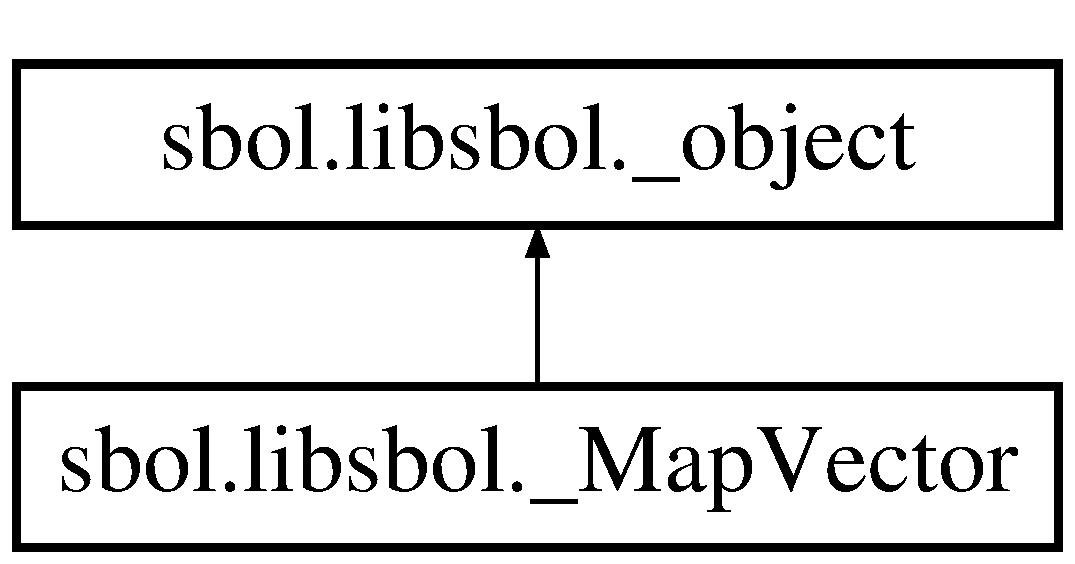
\includegraphics[height=2.000000cm]{classsbol_1_1libsbol_1_1___map_vector}
\end{center}
\end{figure}
\subsection*{Public Member Functions}
\begin{DoxyCompactItemize}
\item 
def {\bfseries iterator} (self)\hypertarget{classsbol_1_1libsbol_1_1___map_vector_aecc7225ec0f27106c0d58aa1a36c7e8f}{}\label{classsbol_1_1libsbol_1_1___map_vector_aecc7225ec0f27106c0d58aa1a36c7e8f}

\item 
def {\bfseries \+\_\+\+\_\+iter\+\_\+\+\_\+} (self)\hypertarget{classsbol_1_1libsbol_1_1___map_vector_a0fcda17ea072904e960bfd351f7be988}{}\label{classsbol_1_1libsbol_1_1___map_vector_a0fcda17ea072904e960bfd351f7be988}

\item 
def {\bfseries \+\_\+\+\_\+nonzero\+\_\+\+\_\+} (self)\hypertarget{classsbol_1_1libsbol_1_1___map_vector_a221a75ba12afa8e57f61c01e548e4327}{}\label{classsbol_1_1libsbol_1_1___map_vector_a221a75ba12afa8e57f61c01e548e4327}

\item 
def {\bfseries \+\_\+\+\_\+bool\+\_\+\+\_\+} (self)\hypertarget{classsbol_1_1libsbol_1_1___map_vector_aeac185aef4ddfacd74c4c6004079bffd}{}\label{classsbol_1_1libsbol_1_1___map_vector_aeac185aef4ddfacd74c4c6004079bffd}

\item 
def {\bfseries \+\_\+\+\_\+len\+\_\+\+\_\+} (self)\hypertarget{classsbol_1_1libsbol_1_1___map_vector_ad43822a639e43cdf6ecbfc6b17f4ed08}{}\label{classsbol_1_1libsbol_1_1___map_vector_ad43822a639e43cdf6ecbfc6b17f4ed08}

\item 
def {\bfseries \+\_\+\+\_\+iter\+\_\+\+\_\+} (self)\hypertarget{classsbol_1_1libsbol_1_1___map_vector_a0fcda17ea072904e960bfd351f7be988}{}\label{classsbol_1_1libsbol_1_1___map_vector_a0fcda17ea072904e960bfd351f7be988}

\item 
def {\bfseries iterkeys} (self)\hypertarget{classsbol_1_1libsbol_1_1___map_vector_a0d2126a19a7c71b682234f3a13723efe}{}\label{classsbol_1_1libsbol_1_1___map_vector_a0d2126a19a7c71b682234f3a13723efe}

\item 
def {\bfseries itervalues} (self)\hypertarget{classsbol_1_1libsbol_1_1___map_vector_a54b0fb7d6330f17d6c67a8c768262c85}{}\label{classsbol_1_1libsbol_1_1___map_vector_a54b0fb7d6330f17d6c67a8c768262c85}

\item 
def {\bfseries iteritems} (self)\hypertarget{classsbol_1_1libsbol_1_1___map_vector_a0e9966d8e4f0ce01aa123efb05adeaab}{}\label{classsbol_1_1libsbol_1_1___map_vector_a0e9966d8e4f0ce01aa123efb05adeaab}

\item 
def {\bfseries \+\_\+\+\_\+getitem\+\_\+\+\_\+} (self, key)\hypertarget{classsbol_1_1libsbol_1_1___map_vector_a891fda170d2c2853dfae47f956124bed}{}\label{classsbol_1_1libsbol_1_1___map_vector_a891fda170d2c2853dfae47f956124bed}

\item 
def {\bfseries \+\_\+\+\_\+delitem\+\_\+\+\_\+} (self, key)\hypertarget{classsbol_1_1libsbol_1_1___map_vector_a8c43f1e8e63f47710dd5ca87beb575ee}{}\label{classsbol_1_1libsbol_1_1___map_vector_a8c43f1e8e63f47710dd5ca87beb575ee}

\item 
def {\bfseries has\+\_\+key} (self, key)\hypertarget{classsbol_1_1libsbol_1_1___map_vector_a98d624ef7e252f1becd77fbd208501a9}{}\label{classsbol_1_1libsbol_1_1___map_vector_a98d624ef7e252f1becd77fbd208501a9}

\item 
def {\bfseries keys} (self)\hypertarget{classsbol_1_1libsbol_1_1___map_vector_ad79024ab7de82c7f8843c2b2a477589f}{}\label{classsbol_1_1libsbol_1_1___map_vector_ad79024ab7de82c7f8843c2b2a477589f}

\item 
def {\bfseries values} (self)\hypertarget{classsbol_1_1libsbol_1_1___map_vector_a0aa1e35c4ff821027aae71f8a69b1322}{}\label{classsbol_1_1libsbol_1_1___map_vector_a0aa1e35c4ff821027aae71f8a69b1322}

\item 
def {\bfseries items} (self)\hypertarget{classsbol_1_1libsbol_1_1___map_vector_ac55e1c12049d165160c7af95c9d6f6b8}{}\label{classsbol_1_1libsbol_1_1___map_vector_ac55e1c12049d165160c7af95c9d6f6b8}

\item 
def {\bfseries \+\_\+\+\_\+contains\+\_\+\+\_\+} (self, key)\hypertarget{classsbol_1_1libsbol_1_1___map_vector_ad6e10df42d2960e5538cb09554932eaa}{}\label{classsbol_1_1libsbol_1_1___map_vector_ad6e10df42d2960e5538cb09554932eaa}

\item 
def {\bfseries key\+\_\+iterator} (self)\hypertarget{classsbol_1_1libsbol_1_1___map_vector_ac881fd7a58d9d158b86ceda43d6349ef}{}\label{classsbol_1_1libsbol_1_1___map_vector_ac881fd7a58d9d158b86ceda43d6349ef}

\item 
def {\bfseries value\+\_\+iterator} (self)\hypertarget{classsbol_1_1libsbol_1_1___map_vector_ac36449449dcdd2bf6174b3661e43776b}{}\label{classsbol_1_1libsbol_1_1___map_vector_ac36449449dcdd2bf6174b3661e43776b}

\item 
def {\bfseries \+\_\+\+\_\+setitem\+\_\+\+\_\+} (self, args)\hypertarget{classsbol_1_1libsbol_1_1___map_vector_aa825b7fe5194ab62777ec2e4da9639df}{}\label{classsbol_1_1libsbol_1_1___map_vector_aa825b7fe5194ab62777ec2e4da9639df}

\item 
def {\bfseries asdict} (self)\hypertarget{classsbol_1_1libsbol_1_1___map_vector_ad37649749fa938459b86baee419be562}{}\label{classsbol_1_1libsbol_1_1___map_vector_ad37649749fa938459b86baee419be562}

\item 
def {\bfseries \+\_\+\+\_\+init\+\_\+\+\_\+} (self, args)\hypertarget{classsbol_1_1libsbol_1_1___map_vector_ad2b09b37e7976add5938cbddc853c7ca}{}\label{classsbol_1_1libsbol_1_1___map_vector_ad2b09b37e7976add5938cbddc853c7ca}

\item 
def {\bfseries empty} (self)\hypertarget{classsbol_1_1libsbol_1_1___map_vector_a0b629590241c477a9dc8c63a7c4585da}{}\label{classsbol_1_1libsbol_1_1___map_vector_a0b629590241c477a9dc8c63a7c4585da}

\item 
def {\bfseries size} (self)\hypertarget{classsbol_1_1libsbol_1_1___map_vector_add9bb69af6f434c8417aaa0da31d6ad0}{}\label{classsbol_1_1libsbol_1_1___map_vector_add9bb69af6f434c8417aaa0da31d6ad0}

\item 
def {\bfseries swap} (self, v)\hypertarget{classsbol_1_1libsbol_1_1___map_vector_a40c59f918a4793e62c930563b4ef693d}{}\label{classsbol_1_1libsbol_1_1___map_vector_a40c59f918a4793e62c930563b4ef693d}

\item 
def {\bfseries begin} (self)\hypertarget{classsbol_1_1libsbol_1_1___map_vector_a44be6bafa7cd6bbf00ca604b45624180}{}\label{classsbol_1_1libsbol_1_1___map_vector_a44be6bafa7cd6bbf00ca604b45624180}

\item 
def {\bfseries end} (self)\hypertarget{classsbol_1_1libsbol_1_1___map_vector_a011a4a30391087a24bfd9bb26002e35f}{}\label{classsbol_1_1libsbol_1_1___map_vector_a011a4a30391087a24bfd9bb26002e35f}

\item 
def {\bfseries rbegin} (self)\hypertarget{classsbol_1_1libsbol_1_1___map_vector_a10d263a8dcd077dd6d152b497a3655e5}{}\label{classsbol_1_1libsbol_1_1___map_vector_a10d263a8dcd077dd6d152b497a3655e5}

\item 
def {\bfseries rend} (self)\hypertarget{classsbol_1_1libsbol_1_1___map_vector_a8681824d11f0922fc9c5f79b5ca92cf3}{}\label{classsbol_1_1libsbol_1_1___map_vector_a8681824d11f0922fc9c5f79b5ca92cf3}

\item 
def {\bfseries clear} (self)\hypertarget{classsbol_1_1libsbol_1_1___map_vector_aaae0fb28e6eb731fabc34151ca582e55}{}\label{classsbol_1_1libsbol_1_1___map_vector_aaae0fb28e6eb731fabc34151ca582e55}

\item 
def {\bfseries get\+\_\+allocator} (self)\hypertarget{classsbol_1_1libsbol_1_1___map_vector_ab3bcd35dcef98cca27a8214ade55ff91}{}\label{classsbol_1_1libsbol_1_1___map_vector_ab3bcd35dcef98cca27a8214ade55ff91}

\item 
def {\bfseries count} (self, x)\hypertarget{classsbol_1_1libsbol_1_1___map_vector_a7b6ebdc9f46f65a35d66009cdcc76fe4}{}\label{classsbol_1_1libsbol_1_1___map_vector_a7b6ebdc9f46f65a35d66009cdcc76fe4}

\item 
def {\bfseries erase} (self, args)\hypertarget{classsbol_1_1libsbol_1_1___map_vector_aa75df5378b257fb4db093ff00e081875}{}\label{classsbol_1_1libsbol_1_1___map_vector_aa75df5378b257fb4db093ff00e081875}

\item 
def {\bfseries find} (self, x)\hypertarget{classsbol_1_1libsbol_1_1___map_vector_af9c22f2cfbe9ab6d9fe6132d57dd8e53}{}\label{classsbol_1_1libsbol_1_1___map_vector_af9c22f2cfbe9ab6d9fe6132d57dd8e53}

\item 
def {\bfseries lower\+\_\+bound} (self, x)\hypertarget{classsbol_1_1libsbol_1_1___map_vector_a0bfdfef50c992793258d5cff28847b03}{}\label{classsbol_1_1libsbol_1_1___map_vector_a0bfdfef50c992793258d5cff28847b03}

\item 
def {\bfseries upper\+\_\+bound} (self, x)\hypertarget{classsbol_1_1libsbol_1_1___map_vector_a96d6e820075087366e0e9744236b4f65}{}\label{classsbol_1_1libsbol_1_1___map_vector_a96d6e820075087366e0e9744236b4f65}

\end{DoxyCompactItemize}
\subsection*{Public Attributes}
\begin{DoxyCompactItemize}
\item 
{\bfseries this}\hypertarget{classsbol_1_1libsbol_1_1___map_vector_a5ba731da8e3be1bdd4f93f7ecceb7859}{}\label{classsbol_1_1libsbol_1_1___map_vector_a5ba731da8e3be1bdd4f93f7ecceb7859}

\end{DoxyCompactItemize}


The documentation for this class was generated from the following file\+:\begin{DoxyCompactItemize}
\item 
libsbol.\+py\end{DoxyCompactItemize}

\hypertarget{classsbol_1_1libsbol_1_1__object}{}\section{sbol.\+libsbol.\+\_\+object Class Reference}
\label{classsbol_1_1libsbol_1_1__object}\index{sbol.\+libsbol.\+\_\+object@{sbol.\+libsbol.\+\_\+object}}
Inheritance diagram for sbol.\+libsbol.\+\_\+object\+:\begin{figure}[H]
\begin{center}
\leavevmode
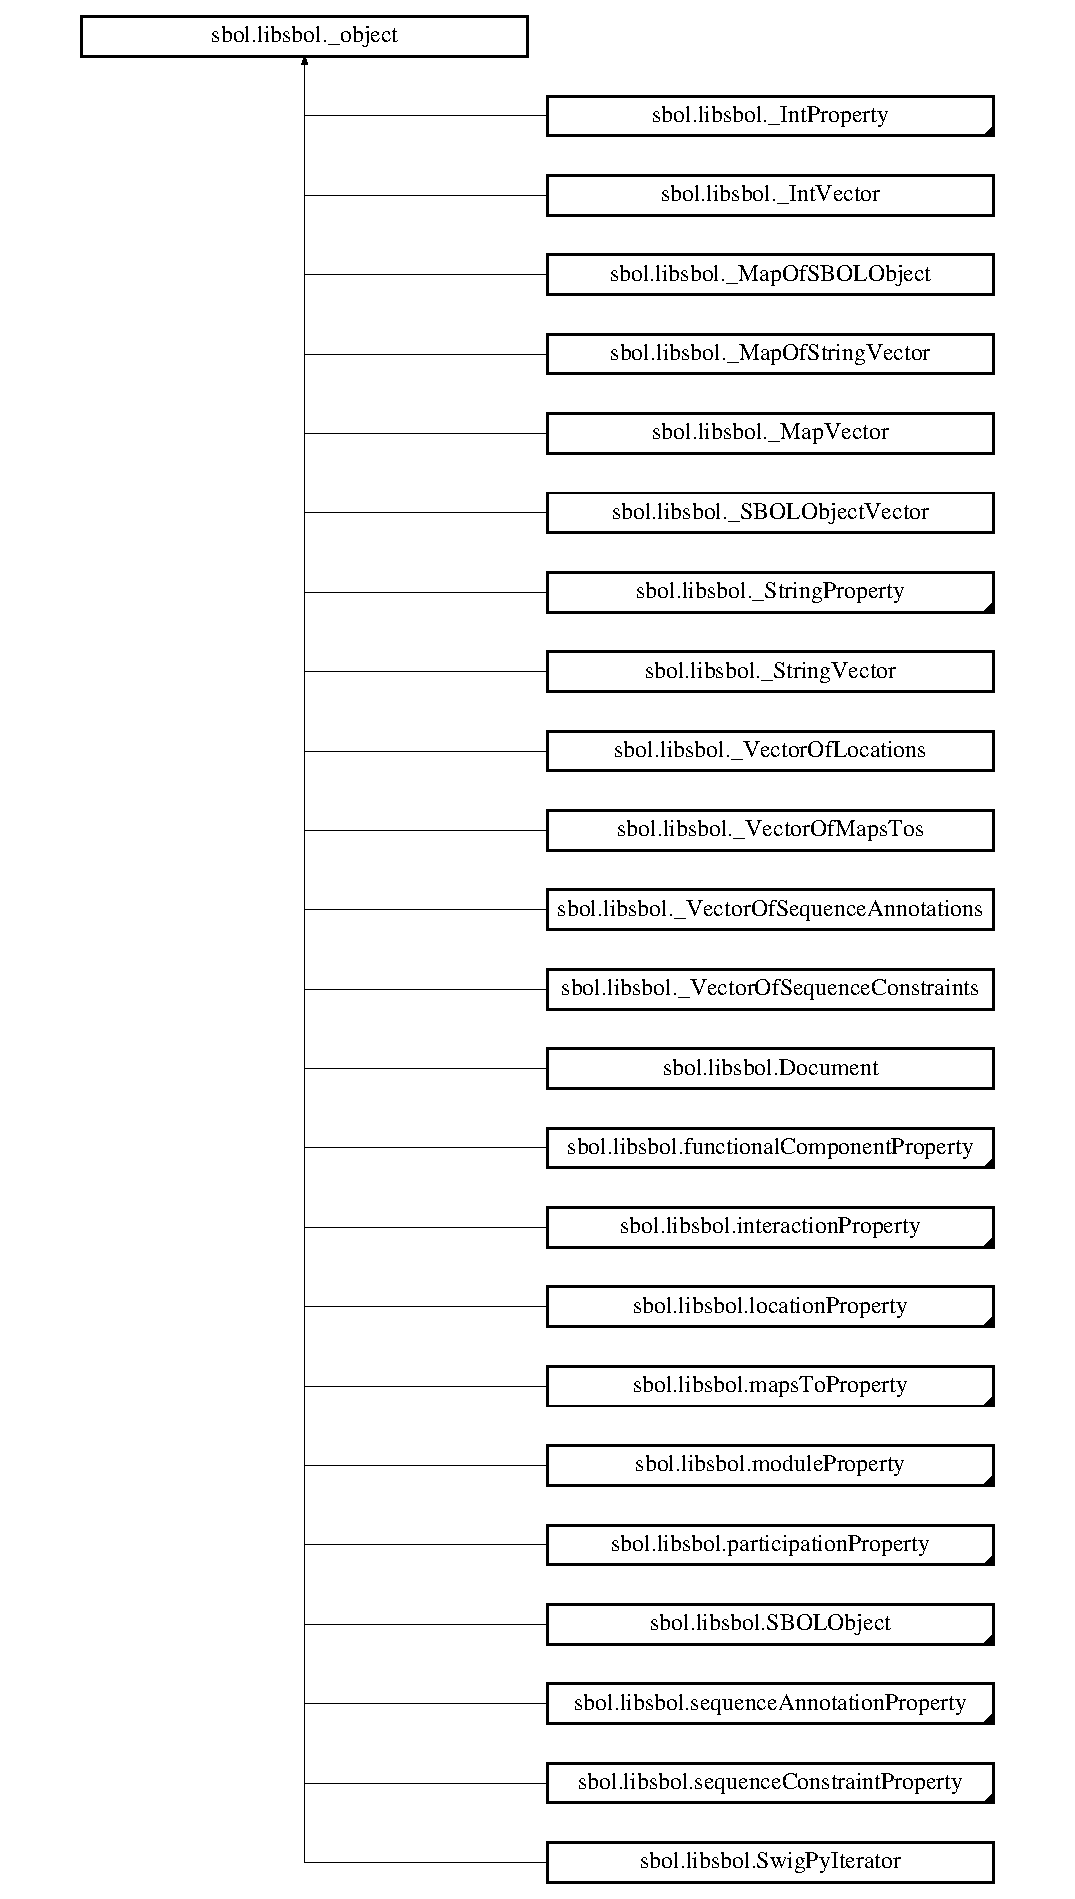
\includegraphics[height=12.000000cm]{classsbol_1_1libsbol_1_1__object}
\end{center}
\end{figure}


The documentation for this class was generated from the following file\+:\begin{DoxyCompactItemize}
\item 
libsbol.\+py\end{DoxyCompactItemize}

\hypertarget{classsbol_1_1libsbol_1_1__owned_location}{}\section{sbol.\+libsbol.\+\_\+owned\+Location Class Reference}
\label{classsbol_1_1libsbol_1_1__owned_location}\index{sbol.\+libsbol.\+\_\+owned\+Location@{sbol.\+libsbol.\+\_\+owned\+Location}}
Inheritance diagram for sbol.\+libsbol.\+\_\+owned\+Location\+:\begin{figure}[H]
\begin{center}
\leavevmode
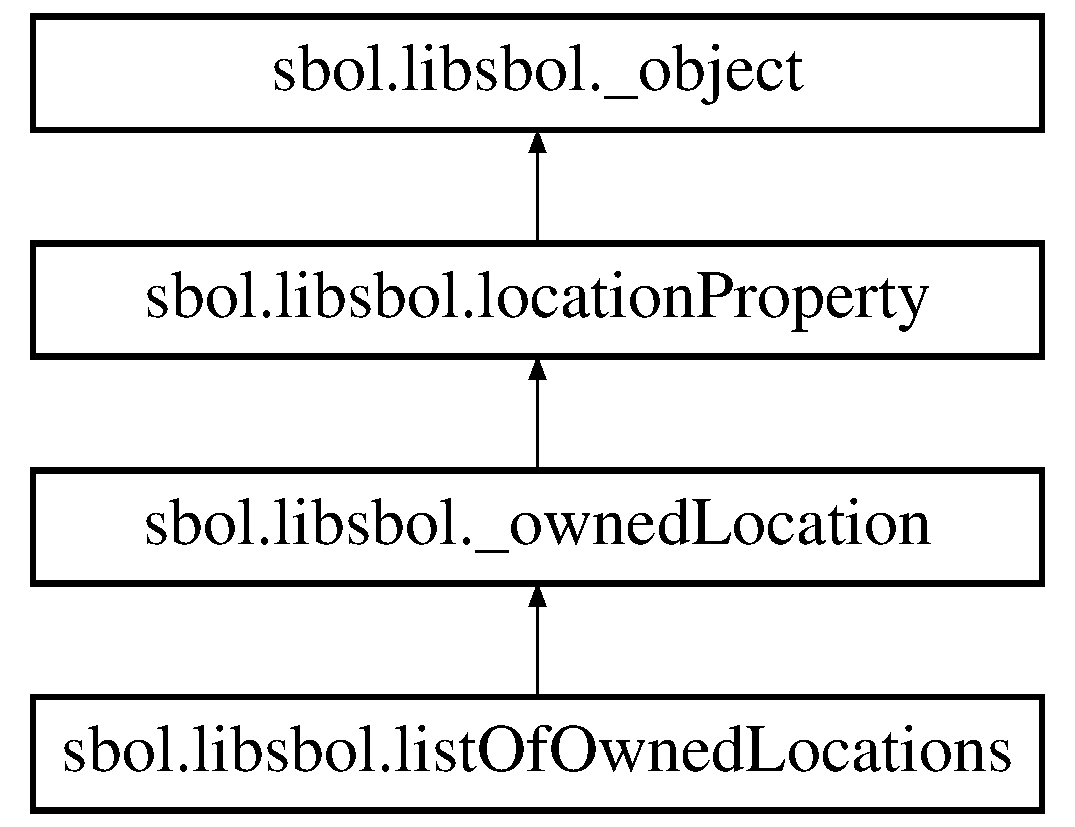
\includegraphics[height=4.000000cm]{classsbol_1_1libsbol_1_1__owned_location}
\end{center}
\end{figure}
\subsection*{Public Member Functions}
\begin{DoxyCompactItemize}
\item 
def \hyperlink{classsbol_1_1libsbol_1_1__owned_location_a6861a39ed03d2c354b03b1a4c44d5e01}{\+\_\+\+\_\+init\+\_\+\+\_\+} (self, args)
\item 
def \hyperlink{classsbol_1_1libsbol_1_1__owned_location_ae83126bfe4c6877e9e673b1b1e2478a5}{add} (self, sbol\+\_\+obj)
\item 
def \hyperlink{classsbol_1_1libsbol_1_1__owned_location_a3881179c0e20cb530dbf75dc1c6d7145}{set} (self, sbol\+\_\+obj)
\item 
def \hyperlink{classsbol_1_1libsbol_1_1__owned_location_a802916b53ae0cb496b2cf47f6a54100a}{get} (self, object\+\_\+id)
\item 
def \hyperlink{classsbol_1_1libsbol_1_1__owned_location_abb0cf446de3bcc395e893f43c69bf21f}{copy} (self)
\item 
def \hyperlink{classsbol_1_1libsbol_1_1__owned_location_a5d5caea3c070c8f9f54d0a7abf426827}{create} (self, args)
\item 
def \hyperlink{classsbol_1_1libsbol_1_1__owned_location_acf8e076d20537be01e4e922a737c24d8}{begin} (self)
\item 
def \hyperlink{classsbol_1_1libsbol_1_1__owned_location_ac92fde8ba671d33c3f4458834ea76fb3}{end} (self)
\item 
def {\bfseries size} (self)\hypertarget{classsbol_1_1libsbol_1_1__owned_location_aa9bb0dc660183df46dba4299517463ac}{}\label{classsbol_1_1libsbol_1_1__owned_location_aa9bb0dc660183df46dba4299517463ac}

\item 
def {\bfseries \+\_\+\+\_\+getitem\+\_\+\+\_\+} (self, args)\hypertarget{classsbol_1_1libsbol_1_1__owned_location_ab12b6455e69bfd804ca0919dd38c2cc0}{}\label{classsbol_1_1libsbol_1_1__owned_location_ab12b6455e69bfd804ca0919dd38c2cc0}

\item 
def {\bfseries \+\_\+\+\_\+iter\+\_\+\+\_\+} (self)\hypertarget{classsbol_1_1libsbol_1_1__owned_location_a8c3e956eab7581fd9177ffcb3a4655e7}{}\label{classsbol_1_1libsbol_1_1__owned_location_a8c3e956eab7581fd9177ffcb3a4655e7}

\item 
def {\bfseries next} (self)\hypertarget{classsbol_1_1libsbol_1_1__owned_location_a0fffa8a557853afa3c7d520016dc2dce}{}\label{classsbol_1_1libsbol_1_1__owned_location_a0fffa8a557853afa3c7d520016dc2dce}

\item 
def {\bfseries \+\_\+\+\_\+len\+\_\+\+\_\+} (self)\hypertarget{classsbol_1_1libsbol_1_1__owned_location_a61192a1cb7ba63dc5403315ddd5d84e5}{}\label{classsbol_1_1libsbol_1_1__owned_location_a61192a1cb7ba63dc5403315ddd5d84e5}

\item 
def \hyperlink{classsbol_1_1libsbol_1_1__owned_location_aa810197acf9b40661452f98abc7e2f3a}{add\+Range} (self, sbol\+\_\+obj)
\item 
def \hyperlink{classsbol_1_1libsbol_1_1__owned_location_a9ab9567a586e5c0ad933a6c6b5052dfd}{get\+Range} (self)
\end{DoxyCompactItemize}
\subsection*{Public Attributes}
\begin{DoxyCompactItemize}
\item 
{\bfseries this}\hypertarget{classsbol_1_1libsbol_1_1__owned_location_ad64da493a48de3f15ea5dc84ba17b3f8}{}\label{classsbol_1_1libsbol_1_1__owned_location_ad64da493a48de3f15ea5dc84ba17b3f8}

\end{DoxyCompactItemize}
\subsection*{Static Public Attributes}
\begin{DoxyCompactItemize}
\item 
{\bfseries python\+\_\+iter} = \+\_\+swig\+\_\+property(\+\_\+libsbol.\+\_\+owned\+Location\+\_\+python\+\_\+iter\+\_\+get, \+\_\+libsbol.\+\_\+owned\+Location\+\_\+python\+\_\+iter\+\_\+set)\hypertarget{classsbol_1_1libsbol_1_1__owned_location_a60a5a5fb1cbe11fd4768fa62583cf5de}{}\label{classsbol_1_1libsbol_1_1__owned_location_a60a5a5fb1cbe11fd4768fa62583cf5de}

\end{DoxyCompactItemize}


\subsection{Constructor \& Destructor Documentation}
\index{sbol\+::libsbol\+::\+\_\+owned\+Location@{sbol\+::libsbol\+::\+\_\+owned\+Location}!\+\_\+\+\_\+init\+\_\+\+\_\+@{\+\_\+\+\_\+init\+\_\+\+\_\+}}
\index{\+\_\+\+\_\+init\+\_\+\+\_\+@{\+\_\+\+\_\+init\+\_\+\+\_\+}!sbol\+::libsbol\+::\+\_\+owned\+Location@{sbol\+::libsbol\+::\+\_\+owned\+Location}}
\subsubsection[{\texorpdfstring{\+\_\+\+\_\+init\+\_\+\+\_\+(self, args)}{__init__(self, args)}}]{\setlength{\rightskip}{0pt plus 5cm}def sbol.\+libsbol.\+\_\+owned\+Location.\+\_\+\+\_\+init\+\_\+\+\_\+ (
\begin{DoxyParamCaption}
\item[{}]{self, }
\item[{}]{args}
\end{DoxyParamCaption}
)}\hypertarget{classsbol_1_1libsbol_1_1__owned_location_a6861a39ed03d2c354b03b1a4c44d5e01}{}\label{classsbol_1_1libsbol_1_1__owned_location_a6861a39ed03d2c354b03b1a4c44d5e01}
\begin{DoxyVerb}sbol::OwnedObject< SBOLClass >::OwnedObject(sbol_type type_uri, void
*property_owner, SBOLObject &first_object) 
\end{DoxyVerb}
 

\subsection{Member Function Documentation}
\index{sbol\+::libsbol\+::\+\_\+owned\+Location@{sbol\+::libsbol\+::\+\_\+owned\+Location}!add@{add}}
\index{add@{add}!sbol\+::libsbol\+::\+\_\+owned\+Location@{sbol\+::libsbol\+::\+\_\+owned\+Location}}
\subsubsection[{\texorpdfstring{add(self, sbol\+\_\+obj)}{add(self, sbol_obj)}}]{\setlength{\rightskip}{0pt plus 5cm}def sbol.\+libsbol.\+\_\+owned\+Location.\+add (
\begin{DoxyParamCaption}
\item[{}]{self, }
\item[{}]{sbol\+\_\+obj}
\end{DoxyParamCaption}
)}\hypertarget{classsbol_1_1libsbol_1_1__owned_location_ae83126bfe4c6877e9e673b1b1e2478a5}{}\label{classsbol_1_1libsbol_1_1__owned_location_ae83126bfe4c6877e9e673b1b1e2478a5}
\begin{DoxyVerb}void
sbol::OwnedObject< SBOLClass >::add(SBOLClass &sbol_obj) 
\end{DoxyVerb}
 \index{sbol\+::libsbol\+::\+\_\+owned\+Location@{sbol\+::libsbol\+::\+\_\+owned\+Location}!add\+Range@{add\+Range}}
\index{add\+Range@{add\+Range}!sbol\+::libsbol\+::\+\_\+owned\+Location@{sbol\+::libsbol\+::\+\_\+owned\+Location}}
\subsubsection[{\texorpdfstring{add\+Range(self, sbol\+\_\+obj)}{addRange(self, sbol_obj)}}]{\setlength{\rightskip}{0pt plus 5cm}def sbol.\+libsbol.\+\_\+owned\+Location.\+add\+Range (
\begin{DoxyParamCaption}
\item[{}]{self, }
\item[{}]{sbol\+\_\+obj}
\end{DoxyParamCaption}
)}\hypertarget{classsbol_1_1libsbol_1_1__owned_location_aa810197acf9b40661452f98abc7e2f3a}{}\label{classsbol_1_1libsbol_1_1__owned_location_aa810197acf9b40661452f98abc7e2f3a}
\begin{DoxyVerb}void
sbol::OwnedObject< SBOLClass >::add(SBOLClass &sbol_obj) 
\end{DoxyVerb}
 \index{sbol\+::libsbol\+::\+\_\+owned\+Location@{sbol\+::libsbol\+::\+\_\+owned\+Location}!begin@{begin}}
\index{begin@{begin}!sbol\+::libsbol\+::\+\_\+owned\+Location@{sbol\+::libsbol\+::\+\_\+owned\+Location}}
\subsubsection[{\texorpdfstring{begin(self)}{begin(self)}}]{\setlength{\rightskip}{0pt plus 5cm}def sbol.\+libsbol.\+\_\+owned\+Location.\+begin (
\begin{DoxyParamCaption}
\item[{}]{self}
\end{DoxyParamCaption}
)}\hypertarget{classsbol_1_1libsbol_1_1__owned_location_acf8e076d20537be01e4e922a737c24d8}{}\label{classsbol_1_1libsbol_1_1__owned_location_acf8e076d20537be01e4e922a737c24d8}
\begin{DoxyVerb}iterator
sbol::OwnedObject< SBOLClass >::begin() 
\end{DoxyVerb}
 \index{sbol\+::libsbol\+::\+\_\+owned\+Location@{sbol\+::libsbol\+::\+\_\+owned\+Location}!copy@{copy}}
\index{copy@{copy}!sbol\+::libsbol\+::\+\_\+owned\+Location@{sbol\+::libsbol\+::\+\_\+owned\+Location}}
\subsubsection[{\texorpdfstring{copy(self)}{copy(self)}}]{\setlength{\rightskip}{0pt plus 5cm}def sbol.\+libsbol.\+\_\+owned\+Location.\+copy (
\begin{DoxyParamCaption}
\item[{}]{self}
\end{DoxyParamCaption}
)}\hypertarget{classsbol_1_1libsbol_1_1__owned_location_abb0cf446de3bcc395e893f43c69bf21f}{}\label{classsbol_1_1libsbol_1_1__owned_location_abb0cf446de3bcc395e893f43c69bf21f}
\begin{DoxyVerb}std::vector<
SBOLClass * > sbol::OwnedObject< SBOLClass >::copy() 
\end{DoxyVerb}
 \index{sbol\+::libsbol\+::\+\_\+owned\+Location@{sbol\+::libsbol\+::\+\_\+owned\+Location}!create@{create}}
\index{create@{create}!sbol\+::libsbol\+::\+\_\+owned\+Location@{sbol\+::libsbol\+::\+\_\+owned\+Location}}
\subsubsection[{\texorpdfstring{create(self, args)}{create(self, args)}}]{\setlength{\rightskip}{0pt plus 5cm}def sbol.\+libsbol.\+\_\+owned\+Location.\+create (
\begin{DoxyParamCaption}
\item[{}]{self, }
\item[{}]{args}
\end{DoxyParamCaption}
)}\hypertarget{classsbol_1_1libsbol_1_1__owned_location_a5d5caea3c070c8f9f54d0a7abf426827}{}\label{classsbol_1_1libsbol_1_1__owned_location_a5d5caea3c070c8f9f54d0a7abf426827}
\begin{DoxyVerb}void
sbol::OwnedObject< SBOLClass >::create(std::string uri_prefix,
std::string display_id, std::string version) 
\end{DoxyVerb}
 \index{sbol\+::libsbol\+::\+\_\+owned\+Location@{sbol\+::libsbol\+::\+\_\+owned\+Location}!end@{end}}
\index{end@{end}!sbol\+::libsbol\+::\+\_\+owned\+Location@{sbol\+::libsbol\+::\+\_\+owned\+Location}}
\subsubsection[{\texorpdfstring{end(self)}{end(self)}}]{\setlength{\rightskip}{0pt plus 5cm}def sbol.\+libsbol.\+\_\+owned\+Location.\+end (
\begin{DoxyParamCaption}
\item[{}]{self}
\end{DoxyParamCaption}
)}\hypertarget{classsbol_1_1libsbol_1_1__owned_location_ac92fde8ba671d33c3f4458834ea76fb3}{}\label{classsbol_1_1libsbol_1_1__owned_location_ac92fde8ba671d33c3f4458834ea76fb3}
\begin{DoxyVerb}iterator
sbol::OwnedObject< SBOLClass >::end() 
\end{DoxyVerb}
 \index{sbol\+::libsbol\+::\+\_\+owned\+Location@{sbol\+::libsbol\+::\+\_\+owned\+Location}!get@{get}}
\index{get@{get}!sbol\+::libsbol\+::\+\_\+owned\+Location@{sbol\+::libsbol\+::\+\_\+owned\+Location}}
\subsubsection[{\texorpdfstring{get(self, object\+\_\+id)}{get(self, object_id)}}]{\setlength{\rightskip}{0pt plus 5cm}def sbol.\+libsbol.\+\_\+owned\+Location.\+get (
\begin{DoxyParamCaption}
\item[{}]{self, }
\item[{}]{object\+\_\+id}
\end{DoxyParamCaption}
)}\hypertarget{classsbol_1_1libsbol_1_1__owned_location_a802916b53ae0cb496b2cf47f6a54100a}{}\label{classsbol_1_1libsbol_1_1__owned_location_a802916b53ae0cb496b2cf47f6a54100a}
\begin{DoxyVerb}SBOLClass &
sbol::OwnedObject< SBOLClass >::get(const std::string object_id) 
\end{DoxyVerb}
 \index{sbol\+::libsbol\+::\+\_\+owned\+Location@{sbol\+::libsbol\+::\+\_\+owned\+Location}!get\+Range@{get\+Range}}
\index{get\+Range@{get\+Range}!sbol\+::libsbol\+::\+\_\+owned\+Location@{sbol\+::libsbol\+::\+\_\+owned\+Location}}
\subsubsection[{\texorpdfstring{get\+Range(self)}{getRange(self)}}]{\setlength{\rightskip}{0pt plus 5cm}def sbol.\+libsbol.\+\_\+owned\+Location.\+get\+Range (
\begin{DoxyParamCaption}
\item[{}]{self}
\end{DoxyParamCaption}
)}\hypertarget{classsbol_1_1libsbol_1_1__owned_location_a9ab9567a586e5c0ad933a6c6b5052dfd}{}\label{classsbol_1_1libsbol_1_1__owned_location_a9ab9567a586e5c0ad933a6c6b5052dfd}
\begin{DoxyVerb}SBOLClass &
sbol::OwnedObject< SBOLClass >::get(const std::string object_id) 
\end{DoxyVerb}
 \index{sbol\+::libsbol\+::\+\_\+owned\+Location@{sbol\+::libsbol\+::\+\_\+owned\+Location}!set@{set}}
\index{set@{set}!sbol\+::libsbol\+::\+\_\+owned\+Location@{sbol\+::libsbol\+::\+\_\+owned\+Location}}
\subsubsection[{\texorpdfstring{set(self, sbol\+\_\+obj)}{set(self, sbol_obj)}}]{\setlength{\rightskip}{0pt plus 5cm}def sbol.\+libsbol.\+\_\+owned\+Location.\+set (
\begin{DoxyParamCaption}
\item[{}]{self, }
\item[{}]{sbol\+\_\+obj}
\end{DoxyParamCaption}
)}\hypertarget{classsbol_1_1libsbol_1_1__owned_location_a3881179c0e20cb530dbf75dc1c6d7145}{}\label{classsbol_1_1libsbol_1_1__owned_location_a3881179c0e20cb530dbf75dc1c6d7145}
\begin{DoxyVerb}void
sbol::OwnedObject< SBOLClass >::set(SBOLClass &sbol_obj) 
\end{DoxyVerb}
 

The documentation for this class was generated from the following file\+:\begin{DoxyCompactItemize}
\item 
libsbol.\+py\end{DoxyCompactItemize}

\hypertarget{classsbol_1_1libsbol_1_1___s_b_o_l_object_vector}{}\section{sbol.\+libsbol.\+\_\+\+S\+B\+O\+L\+Object\+Vector Class Reference}
\label{classsbol_1_1libsbol_1_1___s_b_o_l_object_vector}\index{sbol.\+libsbol.\+\_\+\+S\+B\+O\+L\+Object\+Vector@{sbol.\+libsbol.\+\_\+\+S\+B\+O\+L\+Object\+Vector}}
Inheritance diagram for sbol.\+libsbol.\+\_\+\+S\+B\+O\+L\+Object\+Vector\+:\begin{figure}[H]
\begin{center}
\leavevmode
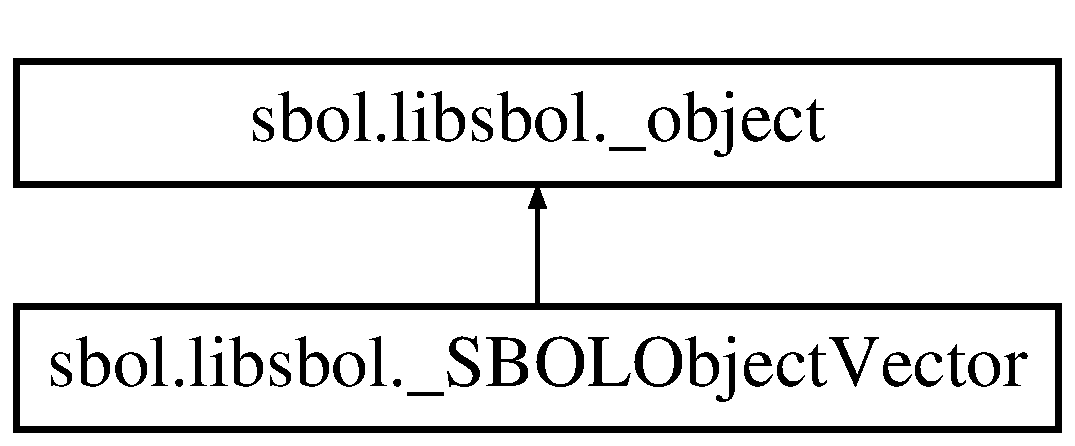
\includegraphics[height=2.000000cm]{classsbol_1_1libsbol_1_1___s_b_o_l_object_vector}
\end{center}
\end{figure}
\subsection*{Public Member Functions}
\begin{DoxyCompactItemize}
\item 
def {\bfseries iterator} (self)\hypertarget{classsbol_1_1libsbol_1_1___s_b_o_l_object_vector_af8585196bd1e1905eafd5b9972e38900}{}\label{classsbol_1_1libsbol_1_1___s_b_o_l_object_vector_af8585196bd1e1905eafd5b9972e38900}

\item 
def {\bfseries \+\_\+\+\_\+iter\+\_\+\+\_\+} (self)\hypertarget{classsbol_1_1libsbol_1_1___s_b_o_l_object_vector_a7dca1bf977fd75179d4aa6b8033b566e}{}\label{classsbol_1_1libsbol_1_1___s_b_o_l_object_vector_a7dca1bf977fd75179d4aa6b8033b566e}

\item 
def {\bfseries \+\_\+\+\_\+nonzero\+\_\+\+\_\+} (self)\hypertarget{classsbol_1_1libsbol_1_1___s_b_o_l_object_vector_a74c57a42c33f638df8e80cc3d23210d4}{}\label{classsbol_1_1libsbol_1_1___s_b_o_l_object_vector_a74c57a42c33f638df8e80cc3d23210d4}

\item 
def {\bfseries \+\_\+\+\_\+bool\+\_\+\+\_\+} (self)\hypertarget{classsbol_1_1libsbol_1_1___s_b_o_l_object_vector_aa2fd12ea3171bc715303d80ec27efc24}{}\label{classsbol_1_1libsbol_1_1___s_b_o_l_object_vector_aa2fd12ea3171bc715303d80ec27efc24}

\item 
def {\bfseries \+\_\+\+\_\+len\+\_\+\+\_\+} (self)\hypertarget{classsbol_1_1libsbol_1_1___s_b_o_l_object_vector_a7a73b554e981e54a2451cf7d423a85ed}{}\label{classsbol_1_1libsbol_1_1___s_b_o_l_object_vector_a7a73b554e981e54a2451cf7d423a85ed}

\item 
def {\bfseries \+\_\+\+\_\+getslice\+\_\+\+\_\+} (self, i, j)\hypertarget{classsbol_1_1libsbol_1_1___s_b_o_l_object_vector_a8f82006ebdcc5cdb33ef05a82de6d116}{}\label{classsbol_1_1libsbol_1_1___s_b_o_l_object_vector_a8f82006ebdcc5cdb33ef05a82de6d116}

\item 
def {\bfseries \+\_\+\+\_\+setslice\+\_\+\+\_\+} (self, args)\hypertarget{classsbol_1_1libsbol_1_1___s_b_o_l_object_vector_a32bf05284af74f7a38f4c56c86220bde}{}\label{classsbol_1_1libsbol_1_1___s_b_o_l_object_vector_a32bf05284af74f7a38f4c56c86220bde}

\item 
def {\bfseries \+\_\+\+\_\+delslice\+\_\+\+\_\+} (self, i, j)\hypertarget{classsbol_1_1libsbol_1_1___s_b_o_l_object_vector_a83331a472b0fe3441f32865b6cdff393}{}\label{classsbol_1_1libsbol_1_1___s_b_o_l_object_vector_a83331a472b0fe3441f32865b6cdff393}

\item 
def {\bfseries \+\_\+\+\_\+delitem\+\_\+\+\_\+} (self, args)\hypertarget{classsbol_1_1libsbol_1_1___s_b_o_l_object_vector_af3bc4767925eb63bc170b76a05e836c7}{}\label{classsbol_1_1libsbol_1_1___s_b_o_l_object_vector_af3bc4767925eb63bc170b76a05e836c7}

\item 
def {\bfseries \+\_\+\+\_\+getitem\+\_\+\+\_\+} (self, args)\hypertarget{classsbol_1_1libsbol_1_1___s_b_o_l_object_vector_aada75e43f1ef91bfb965bdb98f53c8a9}{}\label{classsbol_1_1libsbol_1_1___s_b_o_l_object_vector_aada75e43f1ef91bfb965bdb98f53c8a9}

\item 
def {\bfseries \+\_\+\+\_\+setitem\+\_\+\+\_\+} (self, args)\hypertarget{classsbol_1_1libsbol_1_1___s_b_o_l_object_vector_a9dde77f19cf24d101a4fefcbe25d61fc}{}\label{classsbol_1_1libsbol_1_1___s_b_o_l_object_vector_a9dde77f19cf24d101a4fefcbe25d61fc}

\item 
def {\bfseries pop} (self)\hypertarget{classsbol_1_1libsbol_1_1___s_b_o_l_object_vector_a029c71cc50d0653cb0c669e2a9e6552e}{}\label{classsbol_1_1libsbol_1_1___s_b_o_l_object_vector_a029c71cc50d0653cb0c669e2a9e6552e}

\item 
def {\bfseries append} (self, x)\hypertarget{classsbol_1_1libsbol_1_1___s_b_o_l_object_vector_ab656f3f94cefc34c422817dbc5ca6499}{}\label{classsbol_1_1libsbol_1_1___s_b_o_l_object_vector_ab656f3f94cefc34c422817dbc5ca6499}

\item 
def {\bfseries empty} (self)\hypertarget{classsbol_1_1libsbol_1_1___s_b_o_l_object_vector_ac0dc3b2b1b10eed4f8a45b7c2c343c90}{}\label{classsbol_1_1libsbol_1_1___s_b_o_l_object_vector_ac0dc3b2b1b10eed4f8a45b7c2c343c90}

\item 
def {\bfseries size} (self)\hypertarget{classsbol_1_1libsbol_1_1___s_b_o_l_object_vector_ab3f2c6153b6c4e2077bf3c4df902b90d}{}\label{classsbol_1_1libsbol_1_1___s_b_o_l_object_vector_ab3f2c6153b6c4e2077bf3c4df902b90d}

\item 
def {\bfseries swap} (self, v)\hypertarget{classsbol_1_1libsbol_1_1___s_b_o_l_object_vector_a8d75d285d971ecd72951e5ed1fe07a8a}{}\label{classsbol_1_1libsbol_1_1___s_b_o_l_object_vector_a8d75d285d971ecd72951e5ed1fe07a8a}

\item 
def {\bfseries begin} (self)\hypertarget{classsbol_1_1libsbol_1_1___s_b_o_l_object_vector_a373aa8b66fc194bc5aead5cea73dc607}{}\label{classsbol_1_1libsbol_1_1___s_b_o_l_object_vector_a373aa8b66fc194bc5aead5cea73dc607}

\item 
def {\bfseries end} (self)\hypertarget{classsbol_1_1libsbol_1_1___s_b_o_l_object_vector_aca444944d376774b4fcdc29228065ae3}{}\label{classsbol_1_1libsbol_1_1___s_b_o_l_object_vector_aca444944d376774b4fcdc29228065ae3}

\item 
def {\bfseries rbegin} (self)\hypertarget{classsbol_1_1libsbol_1_1___s_b_o_l_object_vector_a8f67d20df976554274f1191d1b68e630}{}\label{classsbol_1_1libsbol_1_1___s_b_o_l_object_vector_a8f67d20df976554274f1191d1b68e630}

\item 
def {\bfseries rend} (self)\hypertarget{classsbol_1_1libsbol_1_1___s_b_o_l_object_vector_ae32e2e0588cb767b7c0c0bb93bb12bbd}{}\label{classsbol_1_1libsbol_1_1___s_b_o_l_object_vector_ae32e2e0588cb767b7c0c0bb93bb12bbd}

\item 
def {\bfseries clear} (self)\hypertarget{classsbol_1_1libsbol_1_1___s_b_o_l_object_vector_a856bd1b234fd4b528fa1a1c49e051d75}{}\label{classsbol_1_1libsbol_1_1___s_b_o_l_object_vector_a856bd1b234fd4b528fa1a1c49e051d75}

\item 
def {\bfseries get\+\_\+allocator} (self)\hypertarget{classsbol_1_1libsbol_1_1___s_b_o_l_object_vector_a0fc6716dfeb5fcb87b08c140034ee08b}{}\label{classsbol_1_1libsbol_1_1___s_b_o_l_object_vector_a0fc6716dfeb5fcb87b08c140034ee08b}

\item 
def {\bfseries pop\+\_\+back} (self)\hypertarget{classsbol_1_1libsbol_1_1___s_b_o_l_object_vector_aba003ea9f9b33c6361aa2344a9a2782b}{}\label{classsbol_1_1libsbol_1_1___s_b_o_l_object_vector_aba003ea9f9b33c6361aa2344a9a2782b}

\item 
def {\bfseries erase} (self, args)\hypertarget{classsbol_1_1libsbol_1_1___s_b_o_l_object_vector_ad5850bbe5241b6be556e5885cd28c4dd}{}\label{classsbol_1_1libsbol_1_1___s_b_o_l_object_vector_ad5850bbe5241b6be556e5885cd28c4dd}

\item 
def {\bfseries \+\_\+\+\_\+init\+\_\+\+\_\+} (self, args)\hypertarget{classsbol_1_1libsbol_1_1___s_b_o_l_object_vector_ae8db4cc8c2c3ece0df1a45b2eabdd2aa}{}\label{classsbol_1_1libsbol_1_1___s_b_o_l_object_vector_ae8db4cc8c2c3ece0df1a45b2eabdd2aa}

\item 
def {\bfseries push\+\_\+back} (self, x)\hypertarget{classsbol_1_1libsbol_1_1___s_b_o_l_object_vector_a7b027d7eba63711b0b6b7c364e27703a}{}\label{classsbol_1_1libsbol_1_1___s_b_o_l_object_vector_a7b027d7eba63711b0b6b7c364e27703a}

\item 
def {\bfseries front} (self)\hypertarget{classsbol_1_1libsbol_1_1___s_b_o_l_object_vector_acc521ca8bc5ba4e42c475dd45231bf6d}{}\label{classsbol_1_1libsbol_1_1___s_b_o_l_object_vector_acc521ca8bc5ba4e42c475dd45231bf6d}

\item 
def {\bfseries back} (self)\hypertarget{classsbol_1_1libsbol_1_1___s_b_o_l_object_vector_a1796d47c5557ea9f51eae12015cc6c85}{}\label{classsbol_1_1libsbol_1_1___s_b_o_l_object_vector_a1796d47c5557ea9f51eae12015cc6c85}

\item 
def {\bfseries assign} (self, n, x)\hypertarget{classsbol_1_1libsbol_1_1___s_b_o_l_object_vector_a6f3b10d7322c7a79cb4e716a1f52d2a9}{}\label{classsbol_1_1libsbol_1_1___s_b_o_l_object_vector_a6f3b10d7322c7a79cb4e716a1f52d2a9}

\item 
def {\bfseries resize} (self, args)\hypertarget{classsbol_1_1libsbol_1_1___s_b_o_l_object_vector_a86c13ca1bff8f6c036d6a0c1ee99f43c}{}\label{classsbol_1_1libsbol_1_1___s_b_o_l_object_vector_a86c13ca1bff8f6c036d6a0c1ee99f43c}

\item 
def {\bfseries insert} (self, args)\hypertarget{classsbol_1_1libsbol_1_1___s_b_o_l_object_vector_ae8e5c20dfa841d35b32ff56414890aef}{}\label{classsbol_1_1libsbol_1_1___s_b_o_l_object_vector_ae8e5c20dfa841d35b32ff56414890aef}

\item 
def {\bfseries reserve} (self, n)\hypertarget{classsbol_1_1libsbol_1_1___s_b_o_l_object_vector_a830df2899303f532dc8e81bdc4d423cc}{}\label{classsbol_1_1libsbol_1_1___s_b_o_l_object_vector_a830df2899303f532dc8e81bdc4d423cc}

\item 
def {\bfseries capacity} (self)\hypertarget{classsbol_1_1libsbol_1_1___s_b_o_l_object_vector_af25478bda74c4f2b5c5932b8d5bc692f}{}\label{classsbol_1_1libsbol_1_1___s_b_o_l_object_vector_af25478bda74c4f2b5c5932b8d5bc692f}

\end{DoxyCompactItemize}
\subsection*{Public Attributes}
\begin{DoxyCompactItemize}
\item 
{\bfseries this}\hypertarget{classsbol_1_1libsbol_1_1___s_b_o_l_object_vector_a97a19436d79c49e4279bbccc7a50a9fa}{}\label{classsbol_1_1libsbol_1_1___s_b_o_l_object_vector_a97a19436d79c49e4279bbccc7a50a9fa}

\end{DoxyCompactItemize}


The documentation for this class was generated from the following file\+:\begin{DoxyCompactItemize}
\item 
libsbol.\+py\end{DoxyCompactItemize}

\hypertarget{classsbol_1_1libsbol_1_1___string_property}{}\section{sbol.\+libsbol.\+\_\+\+String\+Property Class Reference}
\label{classsbol_1_1libsbol_1_1___string_property}\index{sbol.\+libsbol.\+\_\+\+String\+Property@{sbol.\+libsbol.\+\_\+\+String\+Property}}
Inheritance diagram for sbol.\+libsbol.\+\_\+\+String\+Property\+:\begin{figure}[H]
\begin{center}
\leavevmode
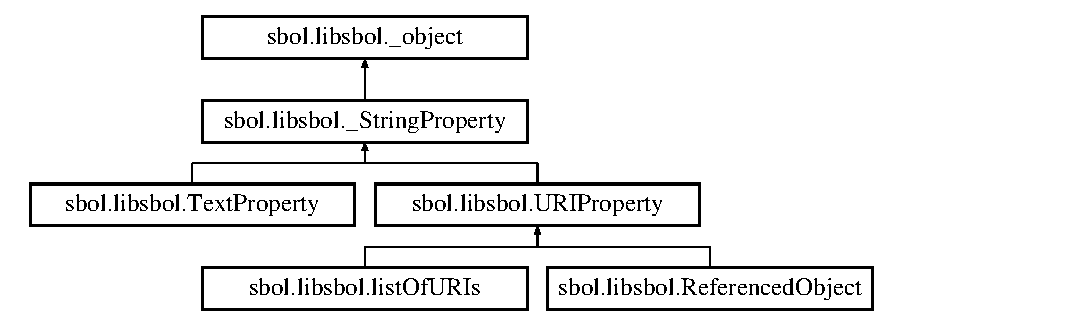
\includegraphics[height=3.929825cm]{classsbol_1_1libsbol_1_1___string_property}
\end{center}
\end{figure}
\subsection*{Public Member Functions}
\begin{DoxyCompactItemize}
\item 
def \hyperlink{classsbol_1_1libsbol_1_1___string_property_a8bba8511f45950730c76c3ed9013f755}{\+\_\+\+\_\+init\+\_\+\+\_\+} (self, args)
\item 
def \hyperlink{classsbol_1_1libsbol_1_1___string_property_a241bb74eea321706f3da7c1a7db870e1}{get\+Type\+U\+RI} (self)
\item 
def \hyperlink{classsbol_1_1libsbol_1_1___string_property_a828226b8e57d704b388ebc90bd0ed62d}{get\+Owner} (self)
\item 
def \hyperlink{classsbol_1_1libsbol_1_1___string_property_a220b61fd41760de94bf4e716b9d7e6dc}{get} (self)
\item 
def \hyperlink{classsbol_1_1libsbol_1_1___string_property_aeccdaf6d2bcb306faf802bb97d030a3b}{add} (self, new\+\_\+value)
\item 
def \hyperlink{classsbol_1_1libsbol_1_1___string_property_a2b31b78c2a8944a5b17886ca46f4f3ec}{set} (self, args)
\item 
def \hyperlink{classsbol_1_1libsbol_1_1___string_property_a65f784ad66fb0c3bbeb9b82abe1c9ec1}{write} (self)
\item 
def \hyperlink{classsbol_1_1libsbol_1_1___string_property_a183e8fc68ca7bb519ce5535d3e1e4712}{validate} (self, arg=None)
\item 
def {\bfseries \+\_\+\+\_\+getitem\+\_\+\+\_\+} (self, n\+Index)\hypertarget{classsbol_1_1libsbol_1_1___string_property_a87a1d3a9428753889af5a65e04480c6a}{}\label{classsbol_1_1libsbol_1_1___string_property_a87a1d3a9428753889af5a65e04480c6a}

\item 
def {\bfseries \+\_\+\+\_\+iter\+\_\+\+\_\+} (self)\hypertarget{classsbol_1_1libsbol_1_1___string_property_a40e2af56f8f3572d8b346c8a9974901f}{}\label{classsbol_1_1libsbol_1_1___string_property_a40e2af56f8f3572d8b346c8a9974901f}

\item 
def {\bfseries next} (self)\hypertarget{classsbol_1_1libsbol_1_1___string_property_ac5178a66d0a6a2940e5635bd4e8652f8}{}\label{classsbol_1_1libsbol_1_1___string_property_ac5178a66d0a6a2940e5635bd4e8652f8}

\item 
def {\bfseries \+\_\+\+\_\+len\+\_\+\+\_\+} (self)\hypertarget{classsbol_1_1libsbol_1_1___string_property_a04d30a9476bf63aa93c173a509e52f00}{}\label{classsbol_1_1libsbol_1_1___string_property_a04d30a9476bf63aa93c173a509e52f00}

\end{DoxyCompactItemize}
\subsection*{Public Attributes}
\begin{DoxyCompactItemize}
\item 
{\bfseries this}\hypertarget{classsbol_1_1libsbol_1_1___string_property_a0b29d0df28983cd19b25732d631d1255}{}\label{classsbol_1_1libsbol_1_1___string_property_a0b29d0df28983cd19b25732d631d1255}

\end{DoxyCompactItemize}


\subsection{Detailed Description}
\begin{DoxyVerb}metafunction for generation of a map of message types to their
associated callbacks.

Usage: Use generate_callback_map<Type>::type to ...

Parameters:
-----------

LiteralType:  The library currently supports Property<string> and
Property<int> specification currently supports integer, string, and
URI literals

C++ includes: property.h 
\end{DoxyVerb}
 

\subsection{Constructor \& Destructor Documentation}
\index{sbol\+::libsbol\+::\+\_\+\+String\+Property@{sbol\+::libsbol\+::\+\_\+\+String\+Property}!\+\_\+\+\_\+init\+\_\+\+\_\+@{\+\_\+\+\_\+init\+\_\+\+\_\+}}
\index{\+\_\+\+\_\+init\+\_\+\+\_\+@{\+\_\+\+\_\+init\+\_\+\+\_\+}!sbol\+::libsbol\+::\+\_\+\+String\+Property@{sbol\+::libsbol\+::\+\_\+\+String\+Property}}
\subsubsection[{\texorpdfstring{\+\_\+\+\_\+init\+\_\+\+\_\+(self, args)}{__init__(self, args)}}]{\setlength{\rightskip}{0pt plus 5cm}def sbol.\+libsbol.\+\_\+\+String\+Property.\+\_\+\+\_\+init\+\_\+\+\_\+ (
\begin{DoxyParamCaption}
\item[{}]{self, }
\item[{}]{args}
\end{DoxyParamCaption}
)}\hypertarget{classsbol_1_1libsbol_1_1___string_property_a8bba8511f45950730c76c3ed9013f755}{}\label{classsbol_1_1libsbol_1_1___string_property_a8bba8511f45950730c76c3ed9013f755}
\begin{DoxyVerb}sbol::Property<
LiteralType >::Property(sbol_type type_uri=UNDEFINED, void
*property_owner=NULL, ValidationRules validation_rules={}) 
\end{DoxyVerb}
 

\subsection{Member Function Documentation}
\index{sbol\+::libsbol\+::\+\_\+\+String\+Property@{sbol\+::libsbol\+::\+\_\+\+String\+Property}!add@{add}}
\index{add@{add}!sbol\+::libsbol\+::\+\_\+\+String\+Property@{sbol\+::libsbol\+::\+\_\+\+String\+Property}}
\subsubsection[{\texorpdfstring{add(self, new\+\_\+value)}{add(self, new_value)}}]{\setlength{\rightskip}{0pt plus 5cm}def sbol.\+libsbol.\+\_\+\+String\+Property.\+add (
\begin{DoxyParamCaption}
\item[{}]{self, }
\item[{}]{new\+\_\+value}
\end{DoxyParamCaption}
)}\hypertarget{classsbol_1_1libsbol_1_1___string_property_aeccdaf6d2bcb306faf802bb97d030a3b}{}\label{classsbol_1_1libsbol_1_1___string_property_aeccdaf6d2bcb306faf802bb97d030a3b}
\begin{DoxyVerb}void sbol::Property<
LiteralType >::add(std::string new_value) 
\end{DoxyVerb}
 \index{sbol\+::libsbol\+::\+\_\+\+String\+Property@{sbol\+::libsbol\+::\+\_\+\+String\+Property}!get@{get}}
\index{get@{get}!sbol\+::libsbol\+::\+\_\+\+String\+Property@{sbol\+::libsbol\+::\+\_\+\+String\+Property}}
\subsubsection[{\texorpdfstring{get(self)}{get(self)}}]{\setlength{\rightskip}{0pt plus 5cm}def sbol.\+libsbol.\+\_\+\+String\+Property.\+get (
\begin{DoxyParamCaption}
\item[{}]{self}
\end{DoxyParamCaption}
)}\hypertarget{classsbol_1_1libsbol_1_1___string_property_a220b61fd41760de94bf4e716b9d7e6dc}{}\label{classsbol_1_1libsbol_1_1___string_property_a220b61fd41760de94bf4e716b9d7e6dc}
\begin{DoxyVerb}std::string
sbol::Property< LiteralType >::get() 
\end{DoxyVerb}
 \index{sbol\+::libsbol\+::\+\_\+\+String\+Property@{sbol\+::libsbol\+::\+\_\+\+String\+Property}!get\+Owner@{get\+Owner}}
\index{get\+Owner@{get\+Owner}!sbol\+::libsbol\+::\+\_\+\+String\+Property@{sbol\+::libsbol\+::\+\_\+\+String\+Property}}
\subsubsection[{\texorpdfstring{get\+Owner(self)}{getOwner(self)}}]{\setlength{\rightskip}{0pt plus 5cm}def sbol.\+libsbol.\+\_\+\+String\+Property.\+get\+Owner (
\begin{DoxyParamCaption}
\item[{}]{self}
\end{DoxyParamCaption}
)}\hypertarget{classsbol_1_1libsbol_1_1___string_property_a828226b8e57d704b388ebc90bd0ed62d}{}\label{classsbol_1_1libsbol_1_1___string_property_a828226b8e57d704b388ebc90bd0ed62d}
\begin{DoxyVerb}SBOLObject &
sbol::Property< LiteralType >::getOwner() 
\end{DoxyVerb}
 \index{sbol\+::libsbol\+::\+\_\+\+String\+Property@{sbol\+::libsbol\+::\+\_\+\+String\+Property}!get\+Type\+U\+RI@{get\+Type\+U\+RI}}
\index{get\+Type\+U\+RI@{get\+Type\+U\+RI}!sbol\+::libsbol\+::\+\_\+\+String\+Property@{sbol\+::libsbol\+::\+\_\+\+String\+Property}}
\subsubsection[{\texorpdfstring{get\+Type\+U\+R\+I(self)}{getTypeURI(self)}}]{\setlength{\rightskip}{0pt plus 5cm}def sbol.\+libsbol.\+\_\+\+String\+Property.\+get\+Type\+U\+RI (
\begin{DoxyParamCaption}
\item[{}]{self}
\end{DoxyParamCaption}
)}\hypertarget{classsbol_1_1libsbol_1_1___string_property_a241bb74eea321706f3da7c1a7db870e1}{}\label{classsbol_1_1libsbol_1_1___string_property_a241bb74eea321706f3da7c1a7db870e1}
\begin{DoxyVerb}sbol_type
sbol::Property< LiteralType >::getTypeURI() 
\end{DoxyVerb}
 \index{sbol\+::libsbol\+::\+\_\+\+String\+Property@{sbol\+::libsbol\+::\+\_\+\+String\+Property}!set@{set}}
\index{set@{set}!sbol\+::libsbol\+::\+\_\+\+String\+Property@{sbol\+::libsbol\+::\+\_\+\+String\+Property}}
\subsubsection[{\texorpdfstring{set(self, args)}{set(self, args)}}]{\setlength{\rightskip}{0pt plus 5cm}def sbol.\+libsbol.\+\_\+\+String\+Property.\+set (
\begin{DoxyParamCaption}
\item[{}]{self, }
\item[{}]{args}
\end{DoxyParamCaption}
)}\hypertarget{classsbol_1_1libsbol_1_1___string_property_a2b31b78c2a8944a5b17886ca46f4f3ec}{}\label{classsbol_1_1libsbol_1_1___string_property_a2b31b78c2a8944a5b17886ca46f4f3ec}
\begin{DoxyVerb}void sbol::Property<
LiteralType >::set(int new_value) 
\end{DoxyVerb}
 \index{sbol\+::libsbol\+::\+\_\+\+String\+Property@{sbol\+::libsbol\+::\+\_\+\+String\+Property}!validate@{validate}}
\index{validate@{validate}!sbol\+::libsbol\+::\+\_\+\+String\+Property@{sbol\+::libsbol\+::\+\_\+\+String\+Property}}
\subsubsection[{\texorpdfstring{validate(self, arg=\+None)}{validate(self, arg=None)}}]{\setlength{\rightskip}{0pt plus 5cm}def sbol.\+libsbol.\+\_\+\+String\+Property.\+validate (
\begin{DoxyParamCaption}
\item[{}]{self, }
\item[{}]{arg = {\ttfamily None}}
\end{DoxyParamCaption}
)}\hypertarget{classsbol_1_1libsbol_1_1___string_property_a183e8fc68ca7bb519ce5535d3e1e4712}{}\label{classsbol_1_1libsbol_1_1___string_property_a183e8fc68ca7bb519ce5535d3e1e4712}
\begin{DoxyVerb}void sbol::Property<
LiteralType >::validate(void *arg=NULL) 
\end{DoxyVerb}
 \index{sbol\+::libsbol\+::\+\_\+\+String\+Property@{sbol\+::libsbol\+::\+\_\+\+String\+Property}!write@{write}}
\index{write@{write}!sbol\+::libsbol\+::\+\_\+\+String\+Property@{sbol\+::libsbol\+::\+\_\+\+String\+Property}}
\subsubsection[{\texorpdfstring{write(self)}{write(self)}}]{\setlength{\rightskip}{0pt plus 5cm}def sbol.\+libsbol.\+\_\+\+String\+Property.\+write (
\begin{DoxyParamCaption}
\item[{}]{self}
\end{DoxyParamCaption}
)}\hypertarget{classsbol_1_1libsbol_1_1___string_property_a65f784ad66fb0c3bbeb9b82abe1c9ec1}{}\label{classsbol_1_1libsbol_1_1___string_property_a65f784ad66fb0c3bbeb9b82abe1c9ec1}
\begin{DoxyVerb}void sbol::Property<
LiteralType >::write() 
\end{DoxyVerb}
 

The documentation for this class was generated from the following file\+:\begin{DoxyCompactItemize}
\item 
libsbol.\+py\end{DoxyCompactItemize}

\hypertarget{classsbol_1_1libsbol_1_1___string_vector}{}\section{sbol.\+libsbol.\+\_\+\+String\+Vector Class Reference}
\label{classsbol_1_1libsbol_1_1___string_vector}\index{sbol.\+libsbol.\+\_\+\+String\+Vector@{sbol.\+libsbol.\+\_\+\+String\+Vector}}
Inheritance diagram for sbol.\+libsbol.\+\_\+\+String\+Vector\+:\begin{figure}[H]
\begin{center}
\leavevmode
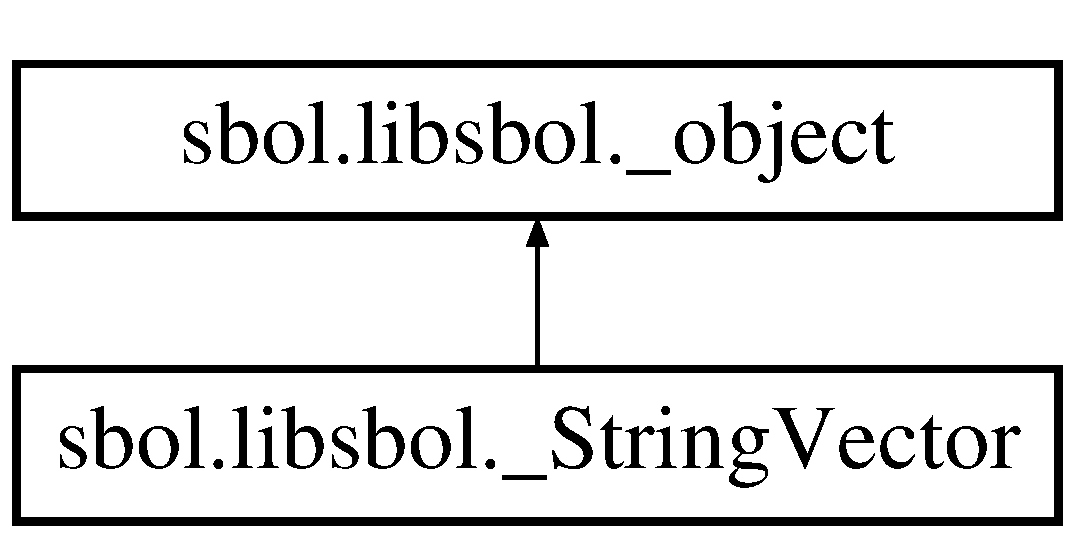
\includegraphics[height=2.000000cm]{classsbol_1_1libsbol_1_1___string_vector}
\end{center}
\end{figure}
\subsection*{Public Member Functions}
\begin{DoxyCompactItemize}
\item 
def {\bfseries iterator} (self)\hypertarget{classsbol_1_1libsbol_1_1___string_vector_adcf4b78a5158410cb7a04b1c838d0f91}{}\label{classsbol_1_1libsbol_1_1___string_vector_adcf4b78a5158410cb7a04b1c838d0f91}

\item 
def {\bfseries \+\_\+\+\_\+iter\+\_\+\+\_\+} (self)\hypertarget{classsbol_1_1libsbol_1_1___string_vector_a5ff613b8096398859fae54512bd4ec90}{}\label{classsbol_1_1libsbol_1_1___string_vector_a5ff613b8096398859fae54512bd4ec90}

\item 
def {\bfseries \+\_\+\+\_\+nonzero\+\_\+\+\_\+} (self)\hypertarget{classsbol_1_1libsbol_1_1___string_vector_a126ffa7be967484c80d04ea51efe6d6a}{}\label{classsbol_1_1libsbol_1_1___string_vector_a126ffa7be967484c80d04ea51efe6d6a}

\item 
def {\bfseries \+\_\+\+\_\+bool\+\_\+\+\_\+} (self)\hypertarget{classsbol_1_1libsbol_1_1___string_vector_a37d22ba629a13b8cf2555b3d384bd7e1}{}\label{classsbol_1_1libsbol_1_1___string_vector_a37d22ba629a13b8cf2555b3d384bd7e1}

\item 
def {\bfseries \+\_\+\+\_\+len\+\_\+\+\_\+} (self)\hypertarget{classsbol_1_1libsbol_1_1___string_vector_ab623629dc843530e0f0643019ec4fd5d}{}\label{classsbol_1_1libsbol_1_1___string_vector_ab623629dc843530e0f0643019ec4fd5d}

\item 
def {\bfseries \+\_\+\+\_\+getslice\+\_\+\+\_\+} (self, i, j)\hypertarget{classsbol_1_1libsbol_1_1___string_vector_ad56e836be207163969fa4cb43a3580f4}{}\label{classsbol_1_1libsbol_1_1___string_vector_ad56e836be207163969fa4cb43a3580f4}

\item 
def {\bfseries \+\_\+\+\_\+setslice\+\_\+\+\_\+} (self, args)\hypertarget{classsbol_1_1libsbol_1_1___string_vector_a4bef7379bade4277aa0fe95cc6fa238f}{}\label{classsbol_1_1libsbol_1_1___string_vector_a4bef7379bade4277aa0fe95cc6fa238f}

\item 
def {\bfseries \+\_\+\+\_\+delslice\+\_\+\+\_\+} (self, i, j)\hypertarget{classsbol_1_1libsbol_1_1___string_vector_a18a25e4a95469a81f679650ea9884c25}{}\label{classsbol_1_1libsbol_1_1___string_vector_a18a25e4a95469a81f679650ea9884c25}

\item 
def {\bfseries \+\_\+\+\_\+delitem\+\_\+\+\_\+} (self, args)\hypertarget{classsbol_1_1libsbol_1_1___string_vector_a9cd8c616b2bbfe96f4c693695fb387fe}{}\label{classsbol_1_1libsbol_1_1___string_vector_a9cd8c616b2bbfe96f4c693695fb387fe}

\item 
def {\bfseries \+\_\+\+\_\+getitem\+\_\+\+\_\+} (self, args)\hypertarget{classsbol_1_1libsbol_1_1___string_vector_a53f254989e6e50a2b8589e061297670b}{}\label{classsbol_1_1libsbol_1_1___string_vector_a53f254989e6e50a2b8589e061297670b}

\item 
def {\bfseries \+\_\+\+\_\+setitem\+\_\+\+\_\+} (self, args)\hypertarget{classsbol_1_1libsbol_1_1___string_vector_ae3b6c4162273fbf318faee091d07fc54}{}\label{classsbol_1_1libsbol_1_1___string_vector_ae3b6c4162273fbf318faee091d07fc54}

\item 
def {\bfseries pop} (self)\hypertarget{classsbol_1_1libsbol_1_1___string_vector_a6a26864416ac1147d2940184579348fd}{}\label{classsbol_1_1libsbol_1_1___string_vector_a6a26864416ac1147d2940184579348fd}

\item 
def {\bfseries append} (self, x)\hypertarget{classsbol_1_1libsbol_1_1___string_vector_ae3466186307c063b4b293632353d22ed}{}\label{classsbol_1_1libsbol_1_1___string_vector_ae3466186307c063b4b293632353d22ed}

\item 
def {\bfseries empty} (self)\hypertarget{classsbol_1_1libsbol_1_1___string_vector_a7803cc6f67d015fb53b4ce5f9428c1e2}{}\label{classsbol_1_1libsbol_1_1___string_vector_a7803cc6f67d015fb53b4ce5f9428c1e2}

\item 
def {\bfseries size} (self)\hypertarget{classsbol_1_1libsbol_1_1___string_vector_a6abfa767aea505d735720e7914e07acd}{}\label{classsbol_1_1libsbol_1_1___string_vector_a6abfa767aea505d735720e7914e07acd}

\item 
def {\bfseries swap} (self, v)\hypertarget{classsbol_1_1libsbol_1_1___string_vector_a730d7af79bff69ab747f149448820cef}{}\label{classsbol_1_1libsbol_1_1___string_vector_a730d7af79bff69ab747f149448820cef}

\item 
def {\bfseries begin} (self)\hypertarget{classsbol_1_1libsbol_1_1___string_vector_a099556799801cd3d5659dc90b93b5f09}{}\label{classsbol_1_1libsbol_1_1___string_vector_a099556799801cd3d5659dc90b93b5f09}

\item 
def {\bfseries end} (self)\hypertarget{classsbol_1_1libsbol_1_1___string_vector_a8467c897bbe6f78b7b77dada748701b4}{}\label{classsbol_1_1libsbol_1_1___string_vector_a8467c897bbe6f78b7b77dada748701b4}

\item 
def {\bfseries rbegin} (self)\hypertarget{classsbol_1_1libsbol_1_1___string_vector_ac37456835acf614f4dc3534d45559eb2}{}\label{classsbol_1_1libsbol_1_1___string_vector_ac37456835acf614f4dc3534d45559eb2}

\item 
def {\bfseries rend} (self)\hypertarget{classsbol_1_1libsbol_1_1___string_vector_a35712bd325551108c9d1771193bfb226}{}\label{classsbol_1_1libsbol_1_1___string_vector_a35712bd325551108c9d1771193bfb226}

\item 
def {\bfseries clear} (self)\hypertarget{classsbol_1_1libsbol_1_1___string_vector_a8d04061a31f628f2ae6e710f9de5867a}{}\label{classsbol_1_1libsbol_1_1___string_vector_a8d04061a31f628f2ae6e710f9de5867a}

\item 
def {\bfseries get\+\_\+allocator} (self)\hypertarget{classsbol_1_1libsbol_1_1___string_vector_a090d575ae5d51c3fda1585c53e6fc661}{}\label{classsbol_1_1libsbol_1_1___string_vector_a090d575ae5d51c3fda1585c53e6fc661}

\item 
def {\bfseries pop\+\_\+back} (self)\hypertarget{classsbol_1_1libsbol_1_1___string_vector_afc5eb6be8914c705195d23dadb1ec658}{}\label{classsbol_1_1libsbol_1_1___string_vector_afc5eb6be8914c705195d23dadb1ec658}

\item 
def {\bfseries erase} (self, args)\hypertarget{classsbol_1_1libsbol_1_1___string_vector_a65ad97d7b2bb4a55713afc023ddd3f22}{}\label{classsbol_1_1libsbol_1_1___string_vector_a65ad97d7b2bb4a55713afc023ddd3f22}

\item 
def {\bfseries \+\_\+\+\_\+init\+\_\+\+\_\+} (self, args)\hypertarget{classsbol_1_1libsbol_1_1___string_vector_a0fb55155369072b6530335fb4decc205}{}\label{classsbol_1_1libsbol_1_1___string_vector_a0fb55155369072b6530335fb4decc205}

\item 
def {\bfseries push\+\_\+back} (self, x)\hypertarget{classsbol_1_1libsbol_1_1___string_vector_af973d6f63e7ef5c0225b31b5679c50c8}{}\label{classsbol_1_1libsbol_1_1___string_vector_af973d6f63e7ef5c0225b31b5679c50c8}

\item 
def {\bfseries front} (self)\hypertarget{classsbol_1_1libsbol_1_1___string_vector_afe20a28101d0f78f4fa139ff5f7e0503}{}\label{classsbol_1_1libsbol_1_1___string_vector_afe20a28101d0f78f4fa139ff5f7e0503}

\item 
def {\bfseries back} (self)\hypertarget{classsbol_1_1libsbol_1_1___string_vector_a357c8f3e011731cc3cb5a83f0e2ce9da}{}\label{classsbol_1_1libsbol_1_1___string_vector_a357c8f3e011731cc3cb5a83f0e2ce9da}

\item 
def {\bfseries assign} (self, n, x)\hypertarget{classsbol_1_1libsbol_1_1___string_vector_a8e0b1f4856c6696d1d727723ff621933}{}\label{classsbol_1_1libsbol_1_1___string_vector_a8e0b1f4856c6696d1d727723ff621933}

\item 
def {\bfseries resize} (self, args)\hypertarget{classsbol_1_1libsbol_1_1___string_vector_a36b1ce93504fc2bc77e237c8ea7925a6}{}\label{classsbol_1_1libsbol_1_1___string_vector_a36b1ce93504fc2bc77e237c8ea7925a6}

\item 
def {\bfseries insert} (self, args)\hypertarget{classsbol_1_1libsbol_1_1___string_vector_ac13b34eba875909df52c27ae3b553273}{}\label{classsbol_1_1libsbol_1_1___string_vector_ac13b34eba875909df52c27ae3b553273}

\item 
def {\bfseries reserve} (self, n)\hypertarget{classsbol_1_1libsbol_1_1___string_vector_a19b0e9a210e84d3feeefd59fda14bbc1}{}\label{classsbol_1_1libsbol_1_1___string_vector_a19b0e9a210e84d3feeefd59fda14bbc1}

\item 
def {\bfseries capacity} (self)\hypertarget{classsbol_1_1libsbol_1_1___string_vector_aaa61d53d57487195ddba40b88e121656}{}\label{classsbol_1_1libsbol_1_1___string_vector_aaa61d53d57487195ddba40b88e121656}

\end{DoxyCompactItemize}
\subsection*{Public Attributes}
\begin{DoxyCompactItemize}
\item 
{\bfseries this}\hypertarget{classsbol_1_1libsbol_1_1___string_vector_ab8b99f7adf045ba6ab00f6d9096873c5}{}\label{classsbol_1_1libsbol_1_1___string_vector_ab8b99f7adf045ba6ab00f6d9096873c5}

\end{DoxyCompactItemize}


The documentation for this class was generated from the following file\+:\begin{DoxyCompactItemize}
\item 
libsbol.\+py\end{DoxyCompactItemize}

\hypertarget{classsbol_1_1libsbol_1_1___vector_of_locations}{}\section{sbol.\+libsbol.\+\_\+\+Vector\+Of\+Locations Class Reference}
\label{classsbol_1_1libsbol_1_1___vector_of_locations}\index{sbol.\+libsbol.\+\_\+\+Vector\+Of\+Locations@{sbol.\+libsbol.\+\_\+\+Vector\+Of\+Locations}}
Inheritance diagram for sbol.\+libsbol.\+\_\+\+Vector\+Of\+Locations\+:\begin{figure}[H]
\begin{center}
\leavevmode
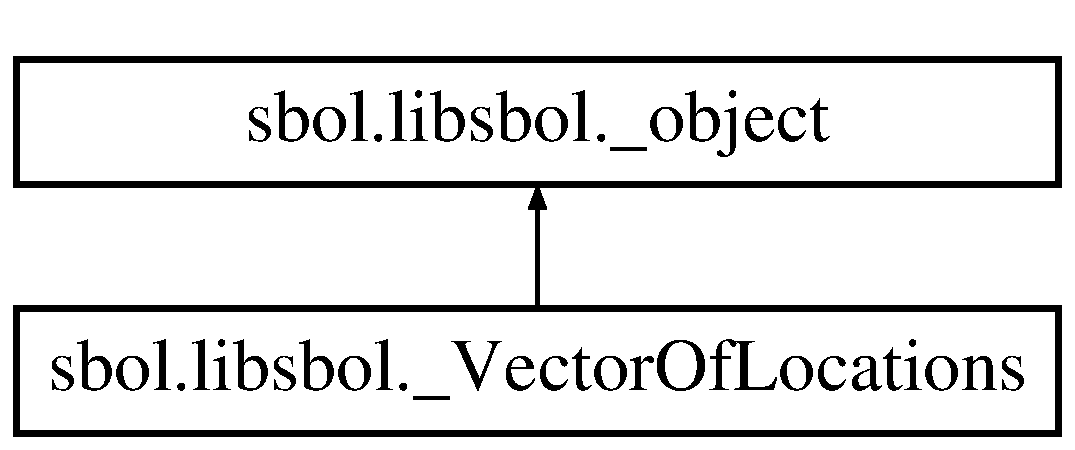
\includegraphics[height=2.000000cm]{classsbol_1_1libsbol_1_1___vector_of_locations}
\end{center}
\end{figure}
\subsection*{Public Member Functions}
\begin{DoxyCompactItemize}
\item 
def {\bfseries iterator} (self)\hypertarget{classsbol_1_1libsbol_1_1___vector_of_locations_a3c2bc77efcc06dcfc33393c10116c826}{}\label{classsbol_1_1libsbol_1_1___vector_of_locations_a3c2bc77efcc06dcfc33393c10116c826}

\item 
def {\bfseries \+\_\+\+\_\+iter\+\_\+\+\_\+} (self)\hypertarget{classsbol_1_1libsbol_1_1___vector_of_locations_aa33c7fff2f9ca05d71c4acc1b545ed96}{}\label{classsbol_1_1libsbol_1_1___vector_of_locations_aa33c7fff2f9ca05d71c4acc1b545ed96}

\item 
def {\bfseries \+\_\+\+\_\+nonzero\+\_\+\+\_\+} (self)\hypertarget{classsbol_1_1libsbol_1_1___vector_of_locations_a54dee65818b1e6b67ae9e9cef0045a47}{}\label{classsbol_1_1libsbol_1_1___vector_of_locations_a54dee65818b1e6b67ae9e9cef0045a47}

\item 
def {\bfseries \+\_\+\+\_\+bool\+\_\+\+\_\+} (self)\hypertarget{classsbol_1_1libsbol_1_1___vector_of_locations_a30305707aa5cbccdf31f0c405850eb15}{}\label{classsbol_1_1libsbol_1_1___vector_of_locations_a30305707aa5cbccdf31f0c405850eb15}

\item 
def {\bfseries \+\_\+\+\_\+len\+\_\+\+\_\+} (self)\hypertarget{classsbol_1_1libsbol_1_1___vector_of_locations_a2e4c3066ca5fe0fc659ce6331563e5e2}{}\label{classsbol_1_1libsbol_1_1___vector_of_locations_a2e4c3066ca5fe0fc659ce6331563e5e2}

\item 
def {\bfseries \+\_\+\+\_\+getslice\+\_\+\+\_\+} (self, i, j)\hypertarget{classsbol_1_1libsbol_1_1___vector_of_locations_aee7520fba59a2f73c05e595939ee7f06}{}\label{classsbol_1_1libsbol_1_1___vector_of_locations_aee7520fba59a2f73c05e595939ee7f06}

\item 
def {\bfseries \+\_\+\+\_\+setslice\+\_\+\+\_\+} (self, args)\hypertarget{classsbol_1_1libsbol_1_1___vector_of_locations_a8fd07f599962ce2beef684f675e3c285}{}\label{classsbol_1_1libsbol_1_1___vector_of_locations_a8fd07f599962ce2beef684f675e3c285}

\item 
def {\bfseries \+\_\+\+\_\+delslice\+\_\+\+\_\+} (self, i, j)\hypertarget{classsbol_1_1libsbol_1_1___vector_of_locations_a6f57fcd7850281b48f165143ef4a4408}{}\label{classsbol_1_1libsbol_1_1___vector_of_locations_a6f57fcd7850281b48f165143ef4a4408}

\item 
def {\bfseries \+\_\+\+\_\+delitem\+\_\+\+\_\+} (self, args)\hypertarget{classsbol_1_1libsbol_1_1___vector_of_locations_aad46360a90671010d69b964acaca497d}{}\label{classsbol_1_1libsbol_1_1___vector_of_locations_aad46360a90671010d69b964acaca497d}

\item 
def {\bfseries \+\_\+\+\_\+getitem\+\_\+\+\_\+} (self, args)\hypertarget{classsbol_1_1libsbol_1_1___vector_of_locations_a90b2e57f177ab54dc3f052d155749fb4}{}\label{classsbol_1_1libsbol_1_1___vector_of_locations_a90b2e57f177ab54dc3f052d155749fb4}

\item 
def {\bfseries \+\_\+\+\_\+setitem\+\_\+\+\_\+} (self, args)\hypertarget{classsbol_1_1libsbol_1_1___vector_of_locations_a1ffd380d894773e39723f7c70ead7246}{}\label{classsbol_1_1libsbol_1_1___vector_of_locations_a1ffd380d894773e39723f7c70ead7246}

\item 
def {\bfseries pop} (self)\hypertarget{classsbol_1_1libsbol_1_1___vector_of_locations_ad00ebdd731897036d2264078b90b11a4}{}\label{classsbol_1_1libsbol_1_1___vector_of_locations_ad00ebdd731897036d2264078b90b11a4}

\item 
def {\bfseries append} (self, x)\hypertarget{classsbol_1_1libsbol_1_1___vector_of_locations_a9bb9638307ce0a5fe4c1a162b80a9520}{}\label{classsbol_1_1libsbol_1_1___vector_of_locations_a9bb9638307ce0a5fe4c1a162b80a9520}

\item 
def {\bfseries empty} (self)\hypertarget{classsbol_1_1libsbol_1_1___vector_of_locations_a8080ac54e19763cadb6e381bcd31ea27}{}\label{classsbol_1_1libsbol_1_1___vector_of_locations_a8080ac54e19763cadb6e381bcd31ea27}

\item 
def {\bfseries size} (self)\hypertarget{classsbol_1_1libsbol_1_1___vector_of_locations_a74ba55a18c0101c12fb1293da0c505c4}{}\label{classsbol_1_1libsbol_1_1___vector_of_locations_a74ba55a18c0101c12fb1293da0c505c4}

\item 
def {\bfseries swap} (self, v)\hypertarget{classsbol_1_1libsbol_1_1___vector_of_locations_af46dc48a0d1d7d30cc48edc716f66ba9}{}\label{classsbol_1_1libsbol_1_1___vector_of_locations_af46dc48a0d1d7d30cc48edc716f66ba9}

\item 
def {\bfseries begin} (self)\hypertarget{classsbol_1_1libsbol_1_1___vector_of_locations_a951252710b0899297c6e8c669aae36d9}{}\label{classsbol_1_1libsbol_1_1___vector_of_locations_a951252710b0899297c6e8c669aae36d9}

\item 
def {\bfseries end} (self)\hypertarget{classsbol_1_1libsbol_1_1___vector_of_locations_aff7df2fba91222fdde4b3d32e8de4713}{}\label{classsbol_1_1libsbol_1_1___vector_of_locations_aff7df2fba91222fdde4b3d32e8de4713}

\item 
def {\bfseries rbegin} (self)\hypertarget{classsbol_1_1libsbol_1_1___vector_of_locations_acd5540adc4cddff96c53e169727c03b9}{}\label{classsbol_1_1libsbol_1_1___vector_of_locations_acd5540adc4cddff96c53e169727c03b9}

\item 
def {\bfseries rend} (self)\hypertarget{classsbol_1_1libsbol_1_1___vector_of_locations_a9cbda8d13adc115379fa16be1b7f7344}{}\label{classsbol_1_1libsbol_1_1___vector_of_locations_a9cbda8d13adc115379fa16be1b7f7344}

\item 
def {\bfseries clear} (self)\hypertarget{classsbol_1_1libsbol_1_1___vector_of_locations_acc3929fcc101ef743101d57c724b0ef6}{}\label{classsbol_1_1libsbol_1_1___vector_of_locations_acc3929fcc101ef743101d57c724b0ef6}

\item 
def {\bfseries get\+\_\+allocator} (self)\hypertarget{classsbol_1_1libsbol_1_1___vector_of_locations_a4059e2dc444b43481e042c79c6383ef5}{}\label{classsbol_1_1libsbol_1_1___vector_of_locations_a4059e2dc444b43481e042c79c6383ef5}

\item 
def {\bfseries pop\+\_\+back} (self)\hypertarget{classsbol_1_1libsbol_1_1___vector_of_locations_a7036bf15aff4bdcf4d3e5fc9ca88c52d}{}\label{classsbol_1_1libsbol_1_1___vector_of_locations_a7036bf15aff4bdcf4d3e5fc9ca88c52d}

\item 
def {\bfseries erase} (self, args)\hypertarget{classsbol_1_1libsbol_1_1___vector_of_locations_ab118ed8e434d47cbbbbfb08783c8f2ae}{}\label{classsbol_1_1libsbol_1_1___vector_of_locations_ab118ed8e434d47cbbbbfb08783c8f2ae}

\item 
def {\bfseries \+\_\+\+\_\+init\+\_\+\+\_\+} (self, args)\hypertarget{classsbol_1_1libsbol_1_1___vector_of_locations_a042b721e41d2eb38d1ecda01f9887120}{}\label{classsbol_1_1libsbol_1_1___vector_of_locations_a042b721e41d2eb38d1ecda01f9887120}

\item 
def {\bfseries push\+\_\+back} (self, x)\hypertarget{classsbol_1_1libsbol_1_1___vector_of_locations_a71daf3fdb62d1b41e05ba0318e177204}{}\label{classsbol_1_1libsbol_1_1___vector_of_locations_a71daf3fdb62d1b41e05ba0318e177204}

\item 
def {\bfseries front} (self)\hypertarget{classsbol_1_1libsbol_1_1___vector_of_locations_a7ec22811cd4e2a8da91f5d305311e158}{}\label{classsbol_1_1libsbol_1_1___vector_of_locations_a7ec22811cd4e2a8da91f5d305311e158}

\item 
def {\bfseries back} (self)\hypertarget{classsbol_1_1libsbol_1_1___vector_of_locations_abaf9788037234058779ec2026f81f490}{}\label{classsbol_1_1libsbol_1_1___vector_of_locations_abaf9788037234058779ec2026f81f490}

\item 
def {\bfseries assign} (self, n, x)\hypertarget{classsbol_1_1libsbol_1_1___vector_of_locations_ae1a8b1169de781e357546fb3398c06da}{}\label{classsbol_1_1libsbol_1_1___vector_of_locations_ae1a8b1169de781e357546fb3398c06da}

\item 
def {\bfseries resize} (self, args)\hypertarget{classsbol_1_1libsbol_1_1___vector_of_locations_a8bfad0f405b13badcf7ff638deea837d}{}\label{classsbol_1_1libsbol_1_1___vector_of_locations_a8bfad0f405b13badcf7ff638deea837d}

\item 
def {\bfseries insert} (self, args)\hypertarget{classsbol_1_1libsbol_1_1___vector_of_locations_ac699f0e28e2e4645fc6b5259607479fd}{}\label{classsbol_1_1libsbol_1_1___vector_of_locations_ac699f0e28e2e4645fc6b5259607479fd}

\item 
def {\bfseries reserve} (self, n)\hypertarget{classsbol_1_1libsbol_1_1___vector_of_locations_a3ad289b07ba7a3ef1f7133583717a8f1}{}\label{classsbol_1_1libsbol_1_1___vector_of_locations_a3ad289b07ba7a3ef1f7133583717a8f1}

\item 
def {\bfseries capacity} (self)\hypertarget{classsbol_1_1libsbol_1_1___vector_of_locations_af7e9865cadf35792f8d60007000767b3}{}\label{classsbol_1_1libsbol_1_1___vector_of_locations_af7e9865cadf35792f8d60007000767b3}

\end{DoxyCompactItemize}
\subsection*{Public Attributes}
\begin{DoxyCompactItemize}
\item 
{\bfseries this}\hypertarget{classsbol_1_1libsbol_1_1___vector_of_locations_a782e8f758b7ff01ca177bd22df6bcef9}{}\label{classsbol_1_1libsbol_1_1___vector_of_locations_a782e8f758b7ff01ca177bd22df6bcef9}

\end{DoxyCompactItemize}


The documentation for this class was generated from the following file\+:\begin{DoxyCompactItemize}
\item 
libsbol.\+py\end{DoxyCompactItemize}

\hypertarget{classsbol_1_1libsbol_1_1___vector_of_maps_tos}{}\section{sbol.\+libsbol.\+\_\+\+Vector\+Of\+Maps\+Tos Class Reference}
\label{classsbol_1_1libsbol_1_1___vector_of_maps_tos}\index{sbol.\+libsbol.\+\_\+\+Vector\+Of\+Maps\+Tos@{sbol.\+libsbol.\+\_\+\+Vector\+Of\+Maps\+Tos}}
Inheritance diagram for sbol.\+libsbol.\+\_\+\+Vector\+Of\+Maps\+Tos\+:\begin{figure}[H]
\begin{center}
\leavevmode
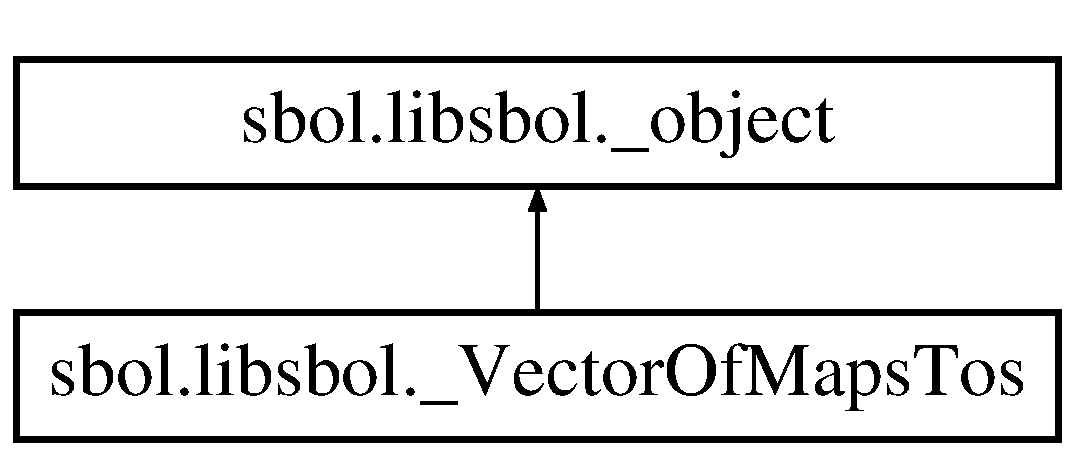
\includegraphics[height=2.000000cm]{classsbol_1_1libsbol_1_1___vector_of_maps_tos}
\end{center}
\end{figure}
\subsection*{Public Member Functions}
\begin{DoxyCompactItemize}
\item 
def {\bfseries iterator} (self)\hypertarget{classsbol_1_1libsbol_1_1___vector_of_maps_tos_ae8edfe2ae44c40b98bf082be8ea974c9}{}\label{classsbol_1_1libsbol_1_1___vector_of_maps_tos_ae8edfe2ae44c40b98bf082be8ea974c9}

\item 
def {\bfseries \+\_\+\+\_\+iter\+\_\+\+\_\+} (self)\hypertarget{classsbol_1_1libsbol_1_1___vector_of_maps_tos_a19d628ddefd52f40861a6ddf438ceca0}{}\label{classsbol_1_1libsbol_1_1___vector_of_maps_tos_a19d628ddefd52f40861a6ddf438ceca0}

\item 
def {\bfseries \+\_\+\+\_\+nonzero\+\_\+\+\_\+} (self)\hypertarget{classsbol_1_1libsbol_1_1___vector_of_maps_tos_a0fe0f24c9c20f893c94d4382996b4abf}{}\label{classsbol_1_1libsbol_1_1___vector_of_maps_tos_a0fe0f24c9c20f893c94d4382996b4abf}

\item 
def {\bfseries \+\_\+\+\_\+bool\+\_\+\+\_\+} (self)\hypertarget{classsbol_1_1libsbol_1_1___vector_of_maps_tos_ac875fc909239469bf012058a2a6f7574}{}\label{classsbol_1_1libsbol_1_1___vector_of_maps_tos_ac875fc909239469bf012058a2a6f7574}

\item 
def {\bfseries \+\_\+\+\_\+len\+\_\+\+\_\+} (self)\hypertarget{classsbol_1_1libsbol_1_1___vector_of_maps_tos_af581bca5a817e3c81a126afe1d0c954c}{}\label{classsbol_1_1libsbol_1_1___vector_of_maps_tos_af581bca5a817e3c81a126afe1d0c954c}

\item 
def {\bfseries \+\_\+\+\_\+getslice\+\_\+\+\_\+} (self, i, j)\hypertarget{classsbol_1_1libsbol_1_1___vector_of_maps_tos_a0e89f67d4302eede78f8e72928207fad}{}\label{classsbol_1_1libsbol_1_1___vector_of_maps_tos_a0e89f67d4302eede78f8e72928207fad}

\item 
def {\bfseries \+\_\+\+\_\+setslice\+\_\+\+\_\+} (self, args)\hypertarget{classsbol_1_1libsbol_1_1___vector_of_maps_tos_aafcdbaf6f176849994c9d5d0c47c44c1}{}\label{classsbol_1_1libsbol_1_1___vector_of_maps_tos_aafcdbaf6f176849994c9d5d0c47c44c1}

\item 
def {\bfseries \+\_\+\+\_\+delslice\+\_\+\+\_\+} (self, i, j)\hypertarget{classsbol_1_1libsbol_1_1___vector_of_maps_tos_a5dcc6e7394d9176f9802ce5172580088}{}\label{classsbol_1_1libsbol_1_1___vector_of_maps_tos_a5dcc6e7394d9176f9802ce5172580088}

\item 
def {\bfseries \+\_\+\+\_\+delitem\+\_\+\+\_\+} (self, args)\hypertarget{classsbol_1_1libsbol_1_1___vector_of_maps_tos_a75a40e82d581f46343aa3f1ee2e0508c}{}\label{classsbol_1_1libsbol_1_1___vector_of_maps_tos_a75a40e82d581f46343aa3f1ee2e0508c}

\item 
def {\bfseries \+\_\+\+\_\+getitem\+\_\+\+\_\+} (self, args)\hypertarget{classsbol_1_1libsbol_1_1___vector_of_maps_tos_ae4107ad2aee09a374586a68584814419}{}\label{classsbol_1_1libsbol_1_1___vector_of_maps_tos_ae4107ad2aee09a374586a68584814419}

\item 
def {\bfseries \+\_\+\+\_\+setitem\+\_\+\+\_\+} (self, args)\hypertarget{classsbol_1_1libsbol_1_1___vector_of_maps_tos_a0d2da71096a0ca4d558f0fc965cb6a97}{}\label{classsbol_1_1libsbol_1_1___vector_of_maps_tos_a0d2da71096a0ca4d558f0fc965cb6a97}

\item 
def {\bfseries pop} (self)\hypertarget{classsbol_1_1libsbol_1_1___vector_of_maps_tos_ac8baba3d232c825b7bf74407e566515e}{}\label{classsbol_1_1libsbol_1_1___vector_of_maps_tos_ac8baba3d232c825b7bf74407e566515e}

\item 
def {\bfseries append} (self, x)\hypertarget{classsbol_1_1libsbol_1_1___vector_of_maps_tos_a1be2c8491c7d70315dedcd5367273fe4}{}\label{classsbol_1_1libsbol_1_1___vector_of_maps_tos_a1be2c8491c7d70315dedcd5367273fe4}

\item 
def {\bfseries empty} (self)\hypertarget{classsbol_1_1libsbol_1_1___vector_of_maps_tos_a9f657e5be3a9df862d90ef4a59df3cbb}{}\label{classsbol_1_1libsbol_1_1___vector_of_maps_tos_a9f657e5be3a9df862d90ef4a59df3cbb}

\item 
def {\bfseries size} (self)\hypertarget{classsbol_1_1libsbol_1_1___vector_of_maps_tos_a0d482f9c3ced9414fb9c9d45f67e0735}{}\label{classsbol_1_1libsbol_1_1___vector_of_maps_tos_a0d482f9c3ced9414fb9c9d45f67e0735}

\item 
def {\bfseries swap} (self, v)\hypertarget{classsbol_1_1libsbol_1_1___vector_of_maps_tos_a5873afc95b864beb8fa82d02094fd0ab}{}\label{classsbol_1_1libsbol_1_1___vector_of_maps_tos_a5873afc95b864beb8fa82d02094fd0ab}

\item 
def {\bfseries begin} (self)\hypertarget{classsbol_1_1libsbol_1_1___vector_of_maps_tos_a24dfe58adbd919aac2bce0dd1e740874}{}\label{classsbol_1_1libsbol_1_1___vector_of_maps_tos_a24dfe58adbd919aac2bce0dd1e740874}

\item 
def {\bfseries end} (self)\hypertarget{classsbol_1_1libsbol_1_1___vector_of_maps_tos_a2f873d642c0f0f651e145e671eeaa52a}{}\label{classsbol_1_1libsbol_1_1___vector_of_maps_tos_a2f873d642c0f0f651e145e671eeaa52a}

\item 
def {\bfseries rbegin} (self)\hypertarget{classsbol_1_1libsbol_1_1___vector_of_maps_tos_ab4f0d55242ca5d314985aa6b23998782}{}\label{classsbol_1_1libsbol_1_1___vector_of_maps_tos_ab4f0d55242ca5d314985aa6b23998782}

\item 
def {\bfseries rend} (self)\hypertarget{classsbol_1_1libsbol_1_1___vector_of_maps_tos_a85a3dfb9b7d869563a2c059e6e664dc0}{}\label{classsbol_1_1libsbol_1_1___vector_of_maps_tos_a85a3dfb9b7d869563a2c059e6e664dc0}

\item 
def {\bfseries clear} (self)\hypertarget{classsbol_1_1libsbol_1_1___vector_of_maps_tos_a6b53a3b8dce90ff2d35bee192fb1a5bc}{}\label{classsbol_1_1libsbol_1_1___vector_of_maps_tos_a6b53a3b8dce90ff2d35bee192fb1a5bc}

\item 
def {\bfseries get\+\_\+allocator} (self)\hypertarget{classsbol_1_1libsbol_1_1___vector_of_maps_tos_a919bf9332b867af2b571078051f7bb75}{}\label{classsbol_1_1libsbol_1_1___vector_of_maps_tos_a919bf9332b867af2b571078051f7bb75}

\item 
def {\bfseries pop\+\_\+back} (self)\hypertarget{classsbol_1_1libsbol_1_1___vector_of_maps_tos_a330a2806b38d8a91fdb4536d89b33a7c}{}\label{classsbol_1_1libsbol_1_1___vector_of_maps_tos_a330a2806b38d8a91fdb4536d89b33a7c}

\item 
def {\bfseries erase} (self, args)\hypertarget{classsbol_1_1libsbol_1_1___vector_of_maps_tos_a04314781d47e0b0ca38b0d8d6afb01de}{}\label{classsbol_1_1libsbol_1_1___vector_of_maps_tos_a04314781d47e0b0ca38b0d8d6afb01de}

\item 
def {\bfseries \+\_\+\+\_\+init\+\_\+\+\_\+} (self, args)\hypertarget{classsbol_1_1libsbol_1_1___vector_of_maps_tos_a8dec49eed0427d88c724e0ddac30c353}{}\label{classsbol_1_1libsbol_1_1___vector_of_maps_tos_a8dec49eed0427d88c724e0ddac30c353}

\item 
def {\bfseries push\+\_\+back} (self, x)\hypertarget{classsbol_1_1libsbol_1_1___vector_of_maps_tos_a4d9341e84c5e596bebfd87b6d37f06fe}{}\label{classsbol_1_1libsbol_1_1___vector_of_maps_tos_a4d9341e84c5e596bebfd87b6d37f06fe}

\item 
def {\bfseries front} (self)\hypertarget{classsbol_1_1libsbol_1_1___vector_of_maps_tos_abb84a5a189f279816b871ecbf1b20b75}{}\label{classsbol_1_1libsbol_1_1___vector_of_maps_tos_abb84a5a189f279816b871ecbf1b20b75}

\item 
def {\bfseries back} (self)\hypertarget{classsbol_1_1libsbol_1_1___vector_of_maps_tos_ac61711487f2ca03995d42bca98bce9fd}{}\label{classsbol_1_1libsbol_1_1___vector_of_maps_tos_ac61711487f2ca03995d42bca98bce9fd}

\item 
def {\bfseries assign} (self, n, x)\hypertarget{classsbol_1_1libsbol_1_1___vector_of_maps_tos_a22d91aad700d484ce6f0fd9d411f81cb}{}\label{classsbol_1_1libsbol_1_1___vector_of_maps_tos_a22d91aad700d484ce6f0fd9d411f81cb}

\item 
def {\bfseries resize} (self, args)\hypertarget{classsbol_1_1libsbol_1_1___vector_of_maps_tos_a09f8aa9445ace6d204e3e60c73f5fb0f}{}\label{classsbol_1_1libsbol_1_1___vector_of_maps_tos_a09f8aa9445ace6d204e3e60c73f5fb0f}

\item 
def {\bfseries insert} (self, args)\hypertarget{classsbol_1_1libsbol_1_1___vector_of_maps_tos_a7bf7f0d5bd09618869e9422de7101655}{}\label{classsbol_1_1libsbol_1_1___vector_of_maps_tos_a7bf7f0d5bd09618869e9422de7101655}

\item 
def {\bfseries reserve} (self, n)\hypertarget{classsbol_1_1libsbol_1_1___vector_of_maps_tos_adbca58de2b426504ebc518e80835e432}{}\label{classsbol_1_1libsbol_1_1___vector_of_maps_tos_adbca58de2b426504ebc518e80835e432}

\item 
def {\bfseries capacity} (self)\hypertarget{classsbol_1_1libsbol_1_1___vector_of_maps_tos_a885a95921e669036bba037cfa2cde709}{}\label{classsbol_1_1libsbol_1_1___vector_of_maps_tos_a885a95921e669036bba037cfa2cde709}

\end{DoxyCompactItemize}
\subsection*{Public Attributes}
\begin{DoxyCompactItemize}
\item 
{\bfseries this}\hypertarget{classsbol_1_1libsbol_1_1___vector_of_maps_tos_ab949dfee74a2cb0c07a1ecccbcaa6097}{}\label{classsbol_1_1libsbol_1_1___vector_of_maps_tos_ab949dfee74a2cb0c07a1ecccbcaa6097}

\end{DoxyCompactItemize}


The documentation for this class was generated from the following file\+:\begin{DoxyCompactItemize}
\item 
libsbol.\+py\end{DoxyCompactItemize}

\hypertarget{classsbol_1_1libsbol_1_1___vector_of_sequence_annotations}{}\section{sbol.\+libsbol.\+\_\+\+Vector\+Of\+Sequence\+Annotations Class Reference}
\label{classsbol_1_1libsbol_1_1___vector_of_sequence_annotations}\index{sbol.\+libsbol.\+\_\+\+Vector\+Of\+Sequence\+Annotations@{sbol.\+libsbol.\+\_\+\+Vector\+Of\+Sequence\+Annotations}}
Inheritance diagram for sbol.\+libsbol.\+\_\+\+Vector\+Of\+Sequence\+Annotations\+:\begin{figure}[H]
\begin{center}
\leavevmode
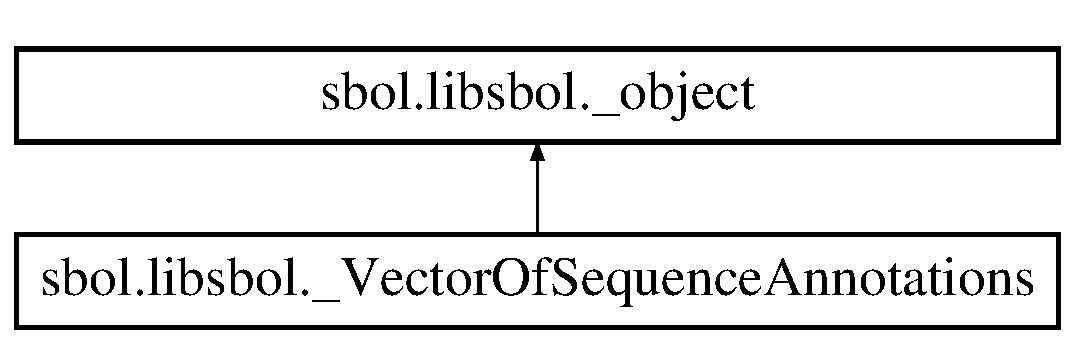
\includegraphics[height=2.000000cm]{classsbol_1_1libsbol_1_1___vector_of_sequence_annotations}
\end{center}
\end{figure}
\subsection*{Public Member Functions}
\begin{DoxyCompactItemize}
\item 
def {\bfseries iterator} (self)\hypertarget{classsbol_1_1libsbol_1_1___vector_of_sequence_annotations_a3227767fb73dd8e033b69aa45e7e9c68}{}\label{classsbol_1_1libsbol_1_1___vector_of_sequence_annotations_a3227767fb73dd8e033b69aa45e7e9c68}

\item 
def {\bfseries \+\_\+\+\_\+iter\+\_\+\+\_\+} (self)\hypertarget{classsbol_1_1libsbol_1_1___vector_of_sequence_annotations_a85d3a703b392e8847400626f08be5f8a}{}\label{classsbol_1_1libsbol_1_1___vector_of_sequence_annotations_a85d3a703b392e8847400626f08be5f8a}

\item 
def {\bfseries \+\_\+\+\_\+nonzero\+\_\+\+\_\+} (self)\hypertarget{classsbol_1_1libsbol_1_1___vector_of_sequence_annotations_a4cdb819e671ca8ebff071f4587bdad1c}{}\label{classsbol_1_1libsbol_1_1___vector_of_sequence_annotations_a4cdb819e671ca8ebff071f4587bdad1c}

\item 
def {\bfseries \+\_\+\+\_\+bool\+\_\+\+\_\+} (self)\hypertarget{classsbol_1_1libsbol_1_1___vector_of_sequence_annotations_ac0250d09428737699dea822417d6ef1d}{}\label{classsbol_1_1libsbol_1_1___vector_of_sequence_annotations_ac0250d09428737699dea822417d6ef1d}

\item 
def {\bfseries \+\_\+\+\_\+len\+\_\+\+\_\+} (self)\hypertarget{classsbol_1_1libsbol_1_1___vector_of_sequence_annotations_a6e1ce6aff41b670bf3c6ca276febf0ed}{}\label{classsbol_1_1libsbol_1_1___vector_of_sequence_annotations_a6e1ce6aff41b670bf3c6ca276febf0ed}

\item 
def {\bfseries \+\_\+\+\_\+getslice\+\_\+\+\_\+} (self, i, j)\hypertarget{classsbol_1_1libsbol_1_1___vector_of_sequence_annotations_a91c25beae46cd054ac24ce6c8ffe6e3e}{}\label{classsbol_1_1libsbol_1_1___vector_of_sequence_annotations_a91c25beae46cd054ac24ce6c8ffe6e3e}

\item 
def {\bfseries \+\_\+\+\_\+setslice\+\_\+\+\_\+} (self, args)\hypertarget{classsbol_1_1libsbol_1_1___vector_of_sequence_annotations_a6067fe987d519387899b9506dbfb7a2f}{}\label{classsbol_1_1libsbol_1_1___vector_of_sequence_annotations_a6067fe987d519387899b9506dbfb7a2f}

\item 
def {\bfseries \+\_\+\+\_\+delslice\+\_\+\+\_\+} (self, i, j)\hypertarget{classsbol_1_1libsbol_1_1___vector_of_sequence_annotations_a9be4494ef7dfb36dce1c7ae722475f6e}{}\label{classsbol_1_1libsbol_1_1___vector_of_sequence_annotations_a9be4494ef7dfb36dce1c7ae722475f6e}

\item 
def {\bfseries \+\_\+\+\_\+delitem\+\_\+\+\_\+} (self, args)\hypertarget{classsbol_1_1libsbol_1_1___vector_of_sequence_annotations_add25b5b01f7d68a95abf2de56a6f3a42}{}\label{classsbol_1_1libsbol_1_1___vector_of_sequence_annotations_add25b5b01f7d68a95abf2de56a6f3a42}

\item 
def {\bfseries \+\_\+\+\_\+getitem\+\_\+\+\_\+} (self, args)\hypertarget{classsbol_1_1libsbol_1_1___vector_of_sequence_annotations_abd56f0c3ad2e7f35eea6d7e18a984ab8}{}\label{classsbol_1_1libsbol_1_1___vector_of_sequence_annotations_abd56f0c3ad2e7f35eea6d7e18a984ab8}

\item 
def {\bfseries \+\_\+\+\_\+setitem\+\_\+\+\_\+} (self, args)\hypertarget{classsbol_1_1libsbol_1_1___vector_of_sequence_annotations_a2b145c26a37b6dc02780580224ff1e03}{}\label{classsbol_1_1libsbol_1_1___vector_of_sequence_annotations_a2b145c26a37b6dc02780580224ff1e03}

\item 
def {\bfseries pop} (self)\hypertarget{classsbol_1_1libsbol_1_1___vector_of_sequence_annotations_a9218cdc469942fbecd6125310f0db7ec}{}\label{classsbol_1_1libsbol_1_1___vector_of_sequence_annotations_a9218cdc469942fbecd6125310f0db7ec}

\item 
def {\bfseries append} (self, x)\hypertarget{classsbol_1_1libsbol_1_1___vector_of_sequence_annotations_a30e6eb01cc1ca7bf86a971dc47776c98}{}\label{classsbol_1_1libsbol_1_1___vector_of_sequence_annotations_a30e6eb01cc1ca7bf86a971dc47776c98}

\item 
def {\bfseries empty} (self)\hypertarget{classsbol_1_1libsbol_1_1___vector_of_sequence_annotations_ad6474af43a81a4545943b85eb016f211}{}\label{classsbol_1_1libsbol_1_1___vector_of_sequence_annotations_ad6474af43a81a4545943b85eb016f211}

\item 
def {\bfseries size} (self)\hypertarget{classsbol_1_1libsbol_1_1___vector_of_sequence_annotations_a1e3bc28232b353302f62a82df482e922}{}\label{classsbol_1_1libsbol_1_1___vector_of_sequence_annotations_a1e3bc28232b353302f62a82df482e922}

\item 
def {\bfseries swap} (self, v)\hypertarget{classsbol_1_1libsbol_1_1___vector_of_sequence_annotations_a623afe7291e739a401531036fccecb09}{}\label{classsbol_1_1libsbol_1_1___vector_of_sequence_annotations_a623afe7291e739a401531036fccecb09}

\item 
def {\bfseries begin} (self)\hypertarget{classsbol_1_1libsbol_1_1___vector_of_sequence_annotations_a3cb0ae2cf1033109b5078276fc32f2ac}{}\label{classsbol_1_1libsbol_1_1___vector_of_sequence_annotations_a3cb0ae2cf1033109b5078276fc32f2ac}

\item 
def {\bfseries end} (self)\hypertarget{classsbol_1_1libsbol_1_1___vector_of_sequence_annotations_ad103f893d6b568ac0d253e5ebe37e40f}{}\label{classsbol_1_1libsbol_1_1___vector_of_sequence_annotations_ad103f893d6b568ac0d253e5ebe37e40f}

\item 
def {\bfseries rbegin} (self)\hypertarget{classsbol_1_1libsbol_1_1___vector_of_sequence_annotations_aa5f0415281e14986215a8ae5344a2f66}{}\label{classsbol_1_1libsbol_1_1___vector_of_sequence_annotations_aa5f0415281e14986215a8ae5344a2f66}

\item 
def {\bfseries rend} (self)\hypertarget{classsbol_1_1libsbol_1_1___vector_of_sequence_annotations_a1ac2df2ebe0c09873b83ca9aa393728c}{}\label{classsbol_1_1libsbol_1_1___vector_of_sequence_annotations_a1ac2df2ebe0c09873b83ca9aa393728c}

\item 
def {\bfseries clear} (self)\hypertarget{classsbol_1_1libsbol_1_1___vector_of_sequence_annotations_acf25a08d586a2650f916ea3a89a55bf3}{}\label{classsbol_1_1libsbol_1_1___vector_of_sequence_annotations_acf25a08d586a2650f916ea3a89a55bf3}

\item 
def {\bfseries get\+\_\+allocator} (self)\hypertarget{classsbol_1_1libsbol_1_1___vector_of_sequence_annotations_ac14bed2548ce0a65901bce561f8a52be}{}\label{classsbol_1_1libsbol_1_1___vector_of_sequence_annotations_ac14bed2548ce0a65901bce561f8a52be}

\item 
def {\bfseries pop\+\_\+back} (self)\hypertarget{classsbol_1_1libsbol_1_1___vector_of_sequence_annotations_ac050a62206fe8b9fa57ce59ef46a0948}{}\label{classsbol_1_1libsbol_1_1___vector_of_sequence_annotations_ac050a62206fe8b9fa57ce59ef46a0948}

\item 
def {\bfseries erase} (self, args)\hypertarget{classsbol_1_1libsbol_1_1___vector_of_sequence_annotations_ab140fd7b6784fc741a65e6ec39e26809}{}\label{classsbol_1_1libsbol_1_1___vector_of_sequence_annotations_ab140fd7b6784fc741a65e6ec39e26809}

\item 
def {\bfseries \+\_\+\+\_\+init\+\_\+\+\_\+} (self, args)\hypertarget{classsbol_1_1libsbol_1_1___vector_of_sequence_annotations_ac0523fb877af650f3b76897a8cbc99f5}{}\label{classsbol_1_1libsbol_1_1___vector_of_sequence_annotations_ac0523fb877af650f3b76897a8cbc99f5}

\item 
def {\bfseries push\+\_\+back} (self, x)\hypertarget{classsbol_1_1libsbol_1_1___vector_of_sequence_annotations_a7cd136de69f2d99ac144aca86460f140}{}\label{classsbol_1_1libsbol_1_1___vector_of_sequence_annotations_a7cd136de69f2d99ac144aca86460f140}

\item 
def {\bfseries front} (self)\hypertarget{classsbol_1_1libsbol_1_1___vector_of_sequence_annotations_a695616d3d61646b5f719735c4fe3b7ca}{}\label{classsbol_1_1libsbol_1_1___vector_of_sequence_annotations_a695616d3d61646b5f719735c4fe3b7ca}

\item 
def {\bfseries back} (self)\hypertarget{classsbol_1_1libsbol_1_1___vector_of_sequence_annotations_a44d72c6ab41175829bfcdaf9888088d0}{}\label{classsbol_1_1libsbol_1_1___vector_of_sequence_annotations_a44d72c6ab41175829bfcdaf9888088d0}

\item 
def {\bfseries assign} (self, n, x)\hypertarget{classsbol_1_1libsbol_1_1___vector_of_sequence_annotations_a533cda2172d6e835b8fa81e852b673a9}{}\label{classsbol_1_1libsbol_1_1___vector_of_sequence_annotations_a533cda2172d6e835b8fa81e852b673a9}

\item 
def {\bfseries resize} (self, args)\hypertarget{classsbol_1_1libsbol_1_1___vector_of_sequence_annotations_a597218921487cf6171c32b2832b4d21c}{}\label{classsbol_1_1libsbol_1_1___vector_of_sequence_annotations_a597218921487cf6171c32b2832b4d21c}

\item 
def {\bfseries insert} (self, args)\hypertarget{classsbol_1_1libsbol_1_1___vector_of_sequence_annotations_a802c7d41a4e4d0d97a05b974416f67e6}{}\label{classsbol_1_1libsbol_1_1___vector_of_sequence_annotations_a802c7d41a4e4d0d97a05b974416f67e6}

\item 
def {\bfseries reserve} (self, n)\hypertarget{classsbol_1_1libsbol_1_1___vector_of_sequence_annotations_a94e1148b11b701d577f497d27488d9a3}{}\label{classsbol_1_1libsbol_1_1___vector_of_sequence_annotations_a94e1148b11b701d577f497d27488d9a3}

\item 
def {\bfseries capacity} (self)\hypertarget{classsbol_1_1libsbol_1_1___vector_of_sequence_annotations_ae44ee549ea2db9d6908ff66c9bc3e5eb}{}\label{classsbol_1_1libsbol_1_1___vector_of_sequence_annotations_ae44ee549ea2db9d6908ff66c9bc3e5eb}

\end{DoxyCompactItemize}
\subsection*{Public Attributes}
\begin{DoxyCompactItemize}
\item 
{\bfseries this}\hypertarget{classsbol_1_1libsbol_1_1___vector_of_sequence_annotations_a83fbee5fcbd7fe80472e2dc34311b23f}{}\label{classsbol_1_1libsbol_1_1___vector_of_sequence_annotations_a83fbee5fcbd7fe80472e2dc34311b23f}

\end{DoxyCompactItemize}


The documentation for this class was generated from the following file\+:\begin{DoxyCompactItemize}
\item 
libsbol.\+py\end{DoxyCompactItemize}

\hypertarget{classsbol_1_1libsbol_1_1___vector_of_sequence_constraints}{}\section{sbol.\+libsbol.\+\_\+\+Vector\+Of\+Sequence\+Constraints Class Reference}
\label{classsbol_1_1libsbol_1_1___vector_of_sequence_constraints}\index{sbol.\+libsbol.\+\_\+\+Vector\+Of\+Sequence\+Constraints@{sbol.\+libsbol.\+\_\+\+Vector\+Of\+Sequence\+Constraints}}
Inheritance diagram for sbol.\+libsbol.\+\_\+\+Vector\+Of\+Sequence\+Constraints\+:\begin{figure}[H]
\begin{center}
\leavevmode
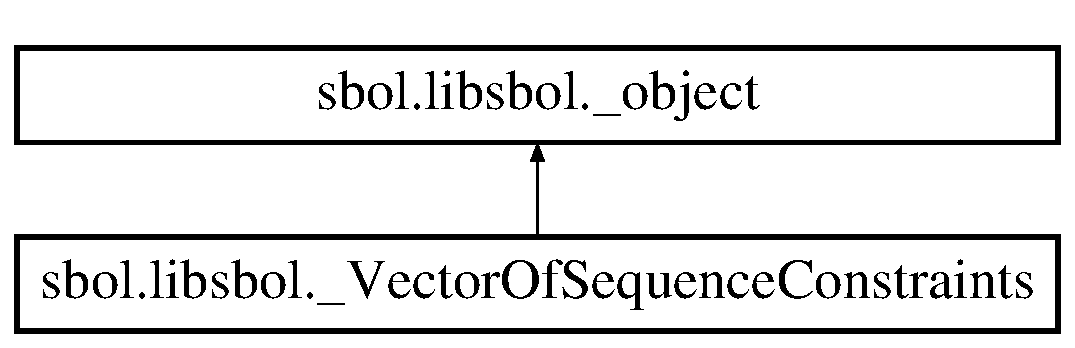
\includegraphics[height=2.000000cm]{classsbol_1_1libsbol_1_1___vector_of_sequence_constraints}
\end{center}
\end{figure}
\subsection*{Public Member Functions}
\begin{DoxyCompactItemize}
\item 
def {\bfseries iterator} (self)\hypertarget{classsbol_1_1libsbol_1_1___vector_of_sequence_constraints_a7c851f2146fb2fcf217e34cc778f9983}{}\label{classsbol_1_1libsbol_1_1___vector_of_sequence_constraints_a7c851f2146fb2fcf217e34cc778f9983}

\item 
def {\bfseries \+\_\+\+\_\+iter\+\_\+\+\_\+} (self)\hypertarget{classsbol_1_1libsbol_1_1___vector_of_sequence_constraints_a09fbd5cf17f65d7174f25b60bdc4b087}{}\label{classsbol_1_1libsbol_1_1___vector_of_sequence_constraints_a09fbd5cf17f65d7174f25b60bdc4b087}

\item 
def {\bfseries \+\_\+\+\_\+nonzero\+\_\+\+\_\+} (self)\hypertarget{classsbol_1_1libsbol_1_1___vector_of_sequence_constraints_a34a0f36110b29d567903bdbddaed6be7}{}\label{classsbol_1_1libsbol_1_1___vector_of_sequence_constraints_a34a0f36110b29d567903bdbddaed6be7}

\item 
def {\bfseries \+\_\+\+\_\+bool\+\_\+\+\_\+} (self)\hypertarget{classsbol_1_1libsbol_1_1___vector_of_sequence_constraints_ae1cc9d65a7416ae735f37531fea0046e}{}\label{classsbol_1_1libsbol_1_1___vector_of_sequence_constraints_ae1cc9d65a7416ae735f37531fea0046e}

\item 
def {\bfseries \+\_\+\+\_\+len\+\_\+\+\_\+} (self)\hypertarget{classsbol_1_1libsbol_1_1___vector_of_sequence_constraints_a30586356c4c5e9620e2e07f50df7071a}{}\label{classsbol_1_1libsbol_1_1___vector_of_sequence_constraints_a30586356c4c5e9620e2e07f50df7071a}

\item 
def {\bfseries \+\_\+\+\_\+getslice\+\_\+\+\_\+} (self, i, j)\hypertarget{classsbol_1_1libsbol_1_1___vector_of_sequence_constraints_a896b07857c5ab101f5f4545855869db4}{}\label{classsbol_1_1libsbol_1_1___vector_of_sequence_constraints_a896b07857c5ab101f5f4545855869db4}

\item 
def {\bfseries \+\_\+\+\_\+setslice\+\_\+\+\_\+} (self, args)\hypertarget{classsbol_1_1libsbol_1_1___vector_of_sequence_constraints_af65afe67533cf4c7e81d59188c5c87b7}{}\label{classsbol_1_1libsbol_1_1___vector_of_sequence_constraints_af65afe67533cf4c7e81d59188c5c87b7}

\item 
def {\bfseries \+\_\+\+\_\+delslice\+\_\+\+\_\+} (self, i, j)\hypertarget{classsbol_1_1libsbol_1_1___vector_of_sequence_constraints_a4e9911457c6d43d88b476b52088a25c8}{}\label{classsbol_1_1libsbol_1_1___vector_of_sequence_constraints_a4e9911457c6d43d88b476b52088a25c8}

\item 
def {\bfseries \+\_\+\+\_\+delitem\+\_\+\+\_\+} (self, args)\hypertarget{classsbol_1_1libsbol_1_1___vector_of_sequence_constraints_a0824e7ddfb9c744834c18dd9edd4853f}{}\label{classsbol_1_1libsbol_1_1___vector_of_sequence_constraints_a0824e7ddfb9c744834c18dd9edd4853f}

\item 
def {\bfseries \+\_\+\+\_\+getitem\+\_\+\+\_\+} (self, args)\hypertarget{classsbol_1_1libsbol_1_1___vector_of_sequence_constraints_add85643d2bcc0328d505f9470e50901d}{}\label{classsbol_1_1libsbol_1_1___vector_of_sequence_constraints_add85643d2bcc0328d505f9470e50901d}

\item 
def {\bfseries \+\_\+\+\_\+setitem\+\_\+\+\_\+} (self, args)\hypertarget{classsbol_1_1libsbol_1_1___vector_of_sequence_constraints_a87a692e6b911a352469b1bb963a86661}{}\label{classsbol_1_1libsbol_1_1___vector_of_sequence_constraints_a87a692e6b911a352469b1bb963a86661}

\item 
def {\bfseries pop} (self)\hypertarget{classsbol_1_1libsbol_1_1___vector_of_sequence_constraints_a0e2eb93fb78b87dcecd82f23c5fe070a}{}\label{classsbol_1_1libsbol_1_1___vector_of_sequence_constraints_a0e2eb93fb78b87dcecd82f23c5fe070a}

\item 
def {\bfseries append} (self, x)\hypertarget{classsbol_1_1libsbol_1_1___vector_of_sequence_constraints_adac0923fd3b6c7894b5f68c227e7e7a2}{}\label{classsbol_1_1libsbol_1_1___vector_of_sequence_constraints_adac0923fd3b6c7894b5f68c227e7e7a2}

\item 
def {\bfseries empty} (self)\hypertarget{classsbol_1_1libsbol_1_1___vector_of_sequence_constraints_aed38931bade6bc8a5d3c14c32635bbee}{}\label{classsbol_1_1libsbol_1_1___vector_of_sequence_constraints_aed38931bade6bc8a5d3c14c32635bbee}

\item 
def {\bfseries size} (self)\hypertarget{classsbol_1_1libsbol_1_1___vector_of_sequence_constraints_a21c602120620afe22c1ed3ab66376214}{}\label{classsbol_1_1libsbol_1_1___vector_of_sequence_constraints_a21c602120620afe22c1ed3ab66376214}

\item 
def {\bfseries swap} (self, v)\hypertarget{classsbol_1_1libsbol_1_1___vector_of_sequence_constraints_afebb478b6c0e669d8cb0f18ecf39968f}{}\label{classsbol_1_1libsbol_1_1___vector_of_sequence_constraints_afebb478b6c0e669d8cb0f18ecf39968f}

\item 
def {\bfseries begin} (self)\hypertarget{classsbol_1_1libsbol_1_1___vector_of_sequence_constraints_aeb2231eb0f20cd76ee46d3448698f237}{}\label{classsbol_1_1libsbol_1_1___vector_of_sequence_constraints_aeb2231eb0f20cd76ee46d3448698f237}

\item 
def {\bfseries end} (self)\hypertarget{classsbol_1_1libsbol_1_1___vector_of_sequence_constraints_aa537964f03aaf15b2135d9490d48fdc2}{}\label{classsbol_1_1libsbol_1_1___vector_of_sequence_constraints_aa537964f03aaf15b2135d9490d48fdc2}

\item 
def {\bfseries rbegin} (self)\hypertarget{classsbol_1_1libsbol_1_1___vector_of_sequence_constraints_acfb8c2af5ff6380f01ba321d73ea0821}{}\label{classsbol_1_1libsbol_1_1___vector_of_sequence_constraints_acfb8c2af5ff6380f01ba321d73ea0821}

\item 
def {\bfseries rend} (self)\hypertarget{classsbol_1_1libsbol_1_1___vector_of_sequence_constraints_ac60635c3d6d47d0839e5ab23b52fc58b}{}\label{classsbol_1_1libsbol_1_1___vector_of_sequence_constraints_ac60635c3d6d47d0839e5ab23b52fc58b}

\item 
def {\bfseries clear} (self)\hypertarget{classsbol_1_1libsbol_1_1___vector_of_sequence_constraints_adc7519209887edf3a5523f441ef2fedf}{}\label{classsbol_1_1libsbol_1_1___vector_of_sequence_constraints_adc7519209887edf3a5523f441ef2fedf}

\item 
def {\bfseries get\+\_\+allocator} (self)\hypertarget{classsbol_1_1libsbol_1_1___vector_of_sequence_constraints_a2d3afe2fd4562f6f75e0cd8e6ba4ccec}{}\label{classsbol_1_1libsbol_1_1___vector_of_sequence_constraints_a2d3afe2fd4562f6f75e0cd8e6ba4ccec}

\item 
def {\bfseries pop\+\_\+back} (self)\hypertarget{classsbol_1_1libsbol_1_1___vector_of_sequence_constraints_a77ac53eb0c71d8eefd143cfd3a930b81}{}\label{classsbol_1_1libsbol_1_1___vector_of_sequence_constraints_a77ac53eb0c71d8eefd143cfd3a930b81}

\item 
def {\bfseries erase} (self, args)\hypertarget{classsbol_1_1libsbol_1_1___vector_of_sequence_constraints_aa17c16192ea3916bae8e2f8ed739bec4}{}\label{classsbol_1_1libsbol_1_1___vector_of_sequence_constraints_aa17c16192ea3916bae8e2f8ed739bec4}

\item 
def {\bfseries \+\_\+\+\_\+init\+\_\+\+\_\+} (self, args)\hypertarget{classsbol_1_1libsbol_1_1___vector_of_sequence_constraints_af08c01815b7acfcfb114b3a1182bc0ca}{}\label{classsbol_1_1libsbol_1_1___vector_of_sequence_constraints_af08c01815b7acfcfb114b3a1182bc0ca}

\item 
def {\bfseries push\+\_\+back} (self, x)\hypertarget{classsbol_1_1libsbol_1_1___vector_of_sequence_constraints_ab8b7d93db4c2db409470c1524521cdb0}{}\label{classsbol_1_1libsbol_1_1___vector_of_sequence_constraints_ab8b7d93db4c2db409470c1524521cdb0}

\item 
def {\bfseries front} (self)\hypertarget{classsbol_1_1libsbol_1_1___vector_of_sequence_constraints_ac7f0de99d41adba327740d7cd0d43427}{}\label{classsbol_1_1libsbol_1_1___vector_of_sequence_constraints_ac7f0de99d41adba327740d7cd0d43427}

\item 
def {\bfseries back} (self)\hypertarget{classsbol_1_1libsbol_1_1___vector_of_sequence_constraints_ac24b2b6b394cfe6a97cf7a27a3b2beaa}{}\label{classsbol_1_1libsbol_1_1___vector_of_sequence_constraints_ac24b2b6b394cfe6a97cf7a27a3b2beaa}

\item 
def {\bfseries assign} (self, n, x)\hypertarget{classsbol_1_1libsbol_1_1___vector_of_sequence_constraints_a308ce2a3b0df5f21c70632ae40f39e4c}{}\label{classsbol_1_1libsbol_1_1___vector_of_sequence_constraints_a308ce2a3b0df5f21c70632ae40f39e4c}

\item 
def {\bfseries resize} (self, args)\hypertarget{classsbol_1_1libsbol_1_1___vector_of_sequence_constraints_a887c687a3b08ec772981316bcea35e18}{}\label{classsbol_1_1libsbol_1_1___vector_of_sequence_constraints_a887c687a3b08ec772981316bcea35e18}

\item 
def {\bfseries insert} (self, args)\hypertarget{classsbol_1_1libsbol_1_1___vector_of_sequence_constraints_ab359ff45b91bd30fc831824a11fb8446}{}\label{classsbol_1_1libsbol_1_1___vector_of_sequence_constraints_ab359ff45b91bd30fc831824a11fb8446}

\item 
def {\bfseries reserve} (self, n)\hypertarget{classsbol_1_1libsbol_1_1___vector_of_sequence_constraints_a085dc469d86be6649ed947cefc52c7e8}{}\label{classsbol_1_1libsbol_1_1___vector_of_sequence_constraints_a085dc469d86be6649ed947cefc52c7e8}

\item 
def {\bfseries capacity} (self)\hypertarget{classsbol_1_1libsbol_1_1___vector_of_sequence_constraints_a9987c086386262a79b32a189a7c9b44f}{}\label{classsbol_1_1libsbol_1_1___vector_of_sequence_constraints_a9987c086386262a79b32a189a7c9b44f}

\end{DoxyCompactItemize}
\subsection*{Public Attributes}
\begin{DoxyCompactItemize}
\item 
{\bfseries this}\hypertarget{classsbol_1_1libsbol_1_1___vector_of_sequence_constraints_af61504edb23f581007485c08c7bdb166}{}\label{classsbol_1_1libsbol_1_1___vector_of_sequence_constraints_af61504edb23f581007485c08c7bdb166}

\end{DoxyCompactItemize}


The documentation for this class was generated from the following file\+:\begin{DoxyCompactItemize}
\item 
libsbol.\+py\end{DoxyCompactItemize}

\hypertarget{classsbol_1_1libsbol_1_1_component}{}\section{sbol.\+libsbol.\+Component Class Reference}
\label{classsbol_1_1libsbol_1_1_component}\index{sbol.\+libsbol.\+Component@{sbol.\+libsbol.\+Component}}
Inheritance diagram for sbol.\+libsbol.\+Component\+:\begin{figure}[H]
\begin{center}
\leavevmode
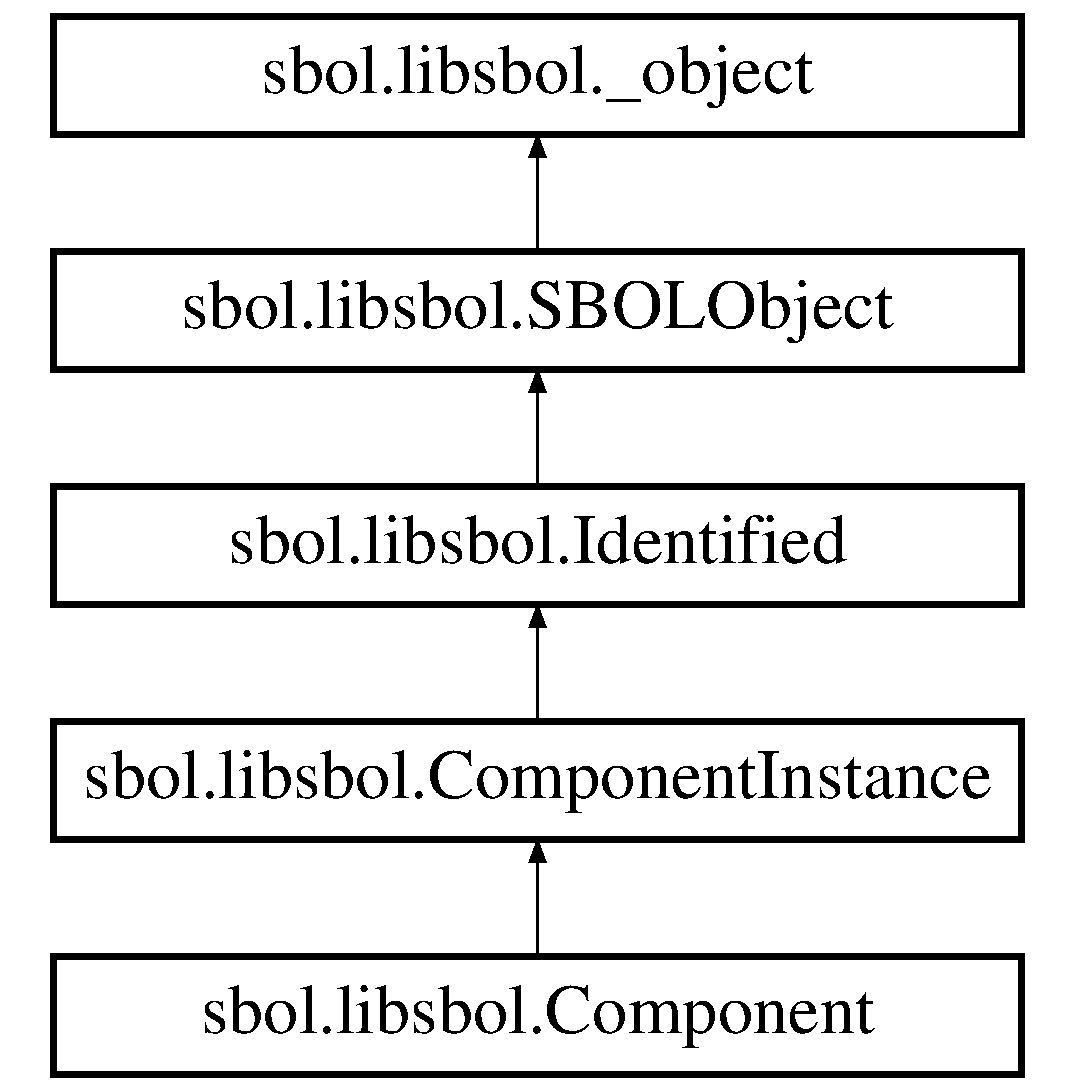
\includegraphics[height=5.000000cm]{classsbol_1_1libsbol_1_1_component}
\end{center}
\end{figure}
\subsection*{Public Member Functions}
\begin{DoxyCompactItemize}
\item 
def \hyperlink{classsbol_1_1libsbol_1_1_component_a577f1e875bd1e8cc428b1c08a01ee814}{\+\_\+\+\_\+init\+\_\+\+\_\+} (self, args)
\end{DoxyCompactItemize}
\subsection*{Public Attributes}
\begin{DoxyCompactItemize}
\item 
{\bfseries this}\hypertarget{classsbol_1_1libsbol_1_1_component_aeb6840b571e8f7a9d809120f5fc459cf}{}\label{classsbol_1_1libsbol_1_1_component_aeb6840b571e8f7a9d809120f5fc459cf}

\end{DoxyCompactItemize}
\subsection*{Additional Inherited Members}


\subsection{Detailed Description}
\begin{DoxyVerb}The Component class is used to compose ComponentDefinition objects into a structural hierarchy (ie, it is a subcomponent). For example, the ComponentDefinition of a gene could contain four Component objects: a promoter, RBS, CDS, and terminator. In turn, the ComponentDefinition of the promoter Component could contain Component objects defined as various operator sites.\end{DoxyVerb}
 

\subsection{Constructor \& Destructor Documentation}
\index{sbol\+::libsbol\+::\+Component@{sbol\+::libsbol\+::\+Component}!\+\_\+\+\_\+init\+\_\+\+\_\+@{\+\_\+\+\_\+init\+\_\+\+\_\+}}
\index{\+\_\+\+\_\+init\+\_\+\+\_\+@{\+\_\+\+\_\+init\+\_\+\+\_\+}!sbol\+::libsbol\+::\+Component@{sbol\+::libsbol\+::\+Component}}
\subsubsection[{\texorpdfstring{\+\_\+\+\_\+init\+\_\+\+\_\+(self, args)}{__init__(self, args)}}]{\setlength{\rightskip}{0pt plus 5cm}def sbol.\+libsbol.\+Component.\+\_\+\+\_\+init\+\_\+\+\_\+ (
\begin{DoxyParamCaption}
\item[{}]{self, }
\item[{}]{args}
\end{DoxyParamCaption}
)}\hypertarget{classsbol_1_1libsbol_1_1_component_a577f1e875bd1e8cc428b1c08a01ee814}{}\label{classsbol_1_1libsbol_1_1_component_a577f1e875bd1e8cc428b1c08a01ee814}
\begin{DoxyVerb}The compliant constructor.  The URI identity of the object is created from the first three arguments
@param uri_prefix The authority for the URI
@param display_id A name for the object that is more human-readable than the URI, but still machine-readable.  The display_id MUST be composed of only alphanumeric or underscore characters and MUST NOT begin with a 26 digit\end{DoxyVerb}
 

The documentation for this class was generated from the following file\+:\begin{DoxyCompactItemize}
\item 
libsbol.\+py\end{DoxyCompactItemize}

\hypertarget{classsbol_1_1libsbol_1_1_component_definition}{}\section{sbol.\+libsbol.\+Component\+Definition Class Reference}
\label{classsbol_1_1libsbol_1_1_component_definition}\index{sbol.\+libsbol.\+Component\+Definition@{sbol.\+libsbol.\+Component\+Definition}}
Inheritance diagram for sbol.\+libsbol.\+Component\+Definition\+:\begin{figure}[H]
\begin{center}
\leavevmode
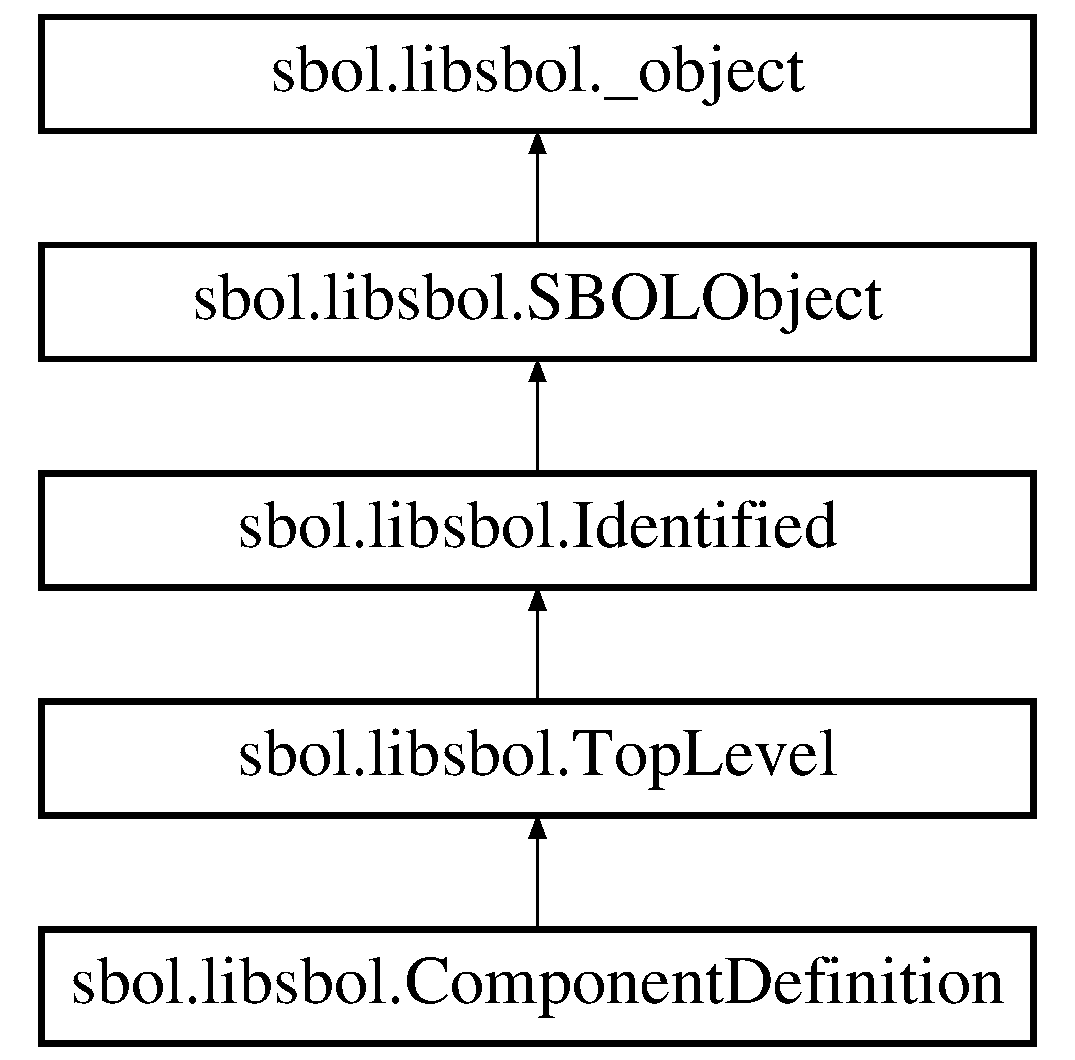
\includegraphics[height=5.000000cm]{classsbol_1_1libsbol_1_1_component_definition}
\end{center}
\end{figure}
\subsection*{Public Member Functions}
\begin{DoxyCompactItemize}
\item 
def \hyperlink{classsbol_1_1libsbol_1_1_component_definition_a0d3c4265de58eb7964a5c0e4c28c61db}{\+\_\+\+\_\+init\+\_\+\+\_\+} (self, args)
\end{DoxyCompactItemize}
\subsection*{Public Attributes}
\begin{DoxyCompactItemize}
\item 
{\bfseries this}\hypertarget{classsbol_1_1libsbol_1_1_component_definition_a24baf76728c9879a059f7ea40499d3cb}{}\label{classsbol_1_1libsbol_1_1_component_definition_a24baf76728c9879a059f7ea40499d3cb}

\end{DoxyCompactItemize}
\subsection*{Static Public Attributes}
\begin{DoxyCompactItemize}
\item 
{\bfseries types} = \+\_\+swig\+\_\+property(\+\_\+libsbol.\+Component\+Definition\+\_\+types\+\_\+get, \+\_\+libsbol.\+Component\+Definition\+\_\+types\+\_\+set)\hypertarget{classsbol_1_1libsbol_1_1_component_definition_a7dd13d02996429b67c134ea0fa88e08c}{}\label{classsbol_1_1libsbol_1_1_component_definition_a7dd13d02996429b67c134ea0fa88e08c}

\item 
{\bfseries roles} = \+\_\+swig\+\_\+property(\+\_\+libsbol.\+Component\+Definition\+\_\+roles\+\_\+get, \+\_\+libsbol.\+Component\+Definition\+\_\+roles\+\_\+set)\hypertarget{classsbol_1_1libsbol_1_1_component_definition_ad137d9e3f64de54247512ae4d68a6e71}{}\label{classsbol_1_1libsbol_1_1_component_definition_ad137d9e3f64de54247512ae4d68a6e71}

\item 
{\bfseries components} = \+\_\+swig\+\_\+property(\+\_\+libsbol.\+Component\+Definition\+\_\+components\+\_\+get, \+\_\+libsbol.\+Component\+Definition\+\_\+components\+\_\+set)\hypertarget{classsbol_1_1libsbol_1_1_component_definition_ab384c2f8615cbc280c31fc03926b3e87}{}\label{classsbol_1_1libsbol_1_1_component_definition_ab384c2f8615cbc280c31fc03926b3e87}

\item 
{\bfseries sequence} = \+\_\+swig\+\_\+property(\+\_\+libsbol.\+Component\+Definition\+\_\+sequence\+\_\+get, \+\_\+libsbol.\+Component\+Definition\+\_\+sequence\+\_\+set)\hypertarget{classsbol_1_1libsbol_1_1_component_definition_a5c051417c0aa9f4d5fe3479281a3d6e0}{}\label{classsbol_1_1libsbol_1_1_component_definition_a5c051417c0aa9f4d5fe3479281a3d6e0}

\item 
{\bfseries sequence\+Annotations} = \+\_\+swig\+\_\+property(\+\_\+libsbol.\+Component\+Definition\+\_\+sequence\+Annotations\+\_\+get, \+\_\+libsbol.\+Component\+Definition\+\_\+sequence\+Annotations\+\_\+set)\hypertarget{classsbol_1_1libsbol_1_1_component_definition_ae9c5beab1424408d7d0eaa3091c6de09}{}\label{classsbol_1_1libsbol_1_1_component_definition_ae9c5beab1424408d7d0eaa3091c6de09}

\item 
{\bfseries sequence\+Constraints} = \+\_\+swig\+\_\+property(\+\_\+libsbol.\+Component\+Definition\+\_\+sequence\+Constraints\+\_\+get, \+\_\+libsbol.\+Component\+Definition\+\_\+sequence\+Constraints\+\_\+set)\hypertarget{classsbol_1_1libsbol_1_1_component_definition_ad437899d9d288901a0cad51d053ef379}{}\label{classsbol_1_1libsbol_1_1_component_definition_ad437899d9d288901a0cad51d053ef379}

\end{DoxyCompactItemize}


\subsection{Constructor \& Destructor Documentation}
\index{sbol\+::libsbol\+::\+Component\+Definition@{sbol\+::libsbol\+::\+Component\+Definition}!\+\_\+\+\_\+init\+\_\+\+\_\+@{\+\_\+\+\_\+init\+\_\+\+\_\+}}
\index{\+\_\+\+\_\+init\+\_\+\+\_\+@{\+\_\+\+\_\+init\+\_\+\+\_\+}!sbol\+::libsbol\+::\+Component\+Definition@{sbol\+::libsbol\+::\+Component\+Definition}}
\subsubsection[{\texorpdfstring{\+\_\+\+\_\+init\+\_\+\+\_\+(self, args)}{__init__(self, args)}}]{\setlength{\rightskip}{0pt plus 5cm}def sbol.\+libsbol.\+Component\+Definition.\+\_\+\+\_\+init\+\_\+\+\_\+ (
\begin{DoxyParamCaption}
\item[{}]{self, }
\item[{}]{args}
\end{DoxyParamCaption}
)}\hypertarget{classsbol_1_1libsbol_1_1_component_definition_a0d3c4265de58eb7964a5c0e4c28c61db}{}\label{classsbol_1_1libsbol_1_1_component_definition_a0d3c4265de58eb7964a5c0e4c28c61db}
\begin{DoxyVerb}sbol::ComponentDefinition::ComponentDefinition(std::string
uri_prefix, std::string display_id, std::string version, std::string
type)\end{DoxyVerb}
 

The documentation for this class was generated from the following file\+:\begin{DoxyCompactItemize}
\item 
libsbol.\+py\end{DoxyCompactItemize}

\hypertarget{classsbol_1_1libsbol_1_1_component_instance}{}\section{sbol.\+libsbol.\+Component\+Instance Class Reference}
\label{classsbol_1_1libsbol_1_1_component_instance}\index{sbol.\+libsbol.\+Component\+Instance@{sbol.\+libsbol.\+Component\+Instance}}
Inheritance diagram for sbol.\+libsbol.\+Component\+Instance\+:\begin{figure}[H]
\begin{center}
\leavevmode
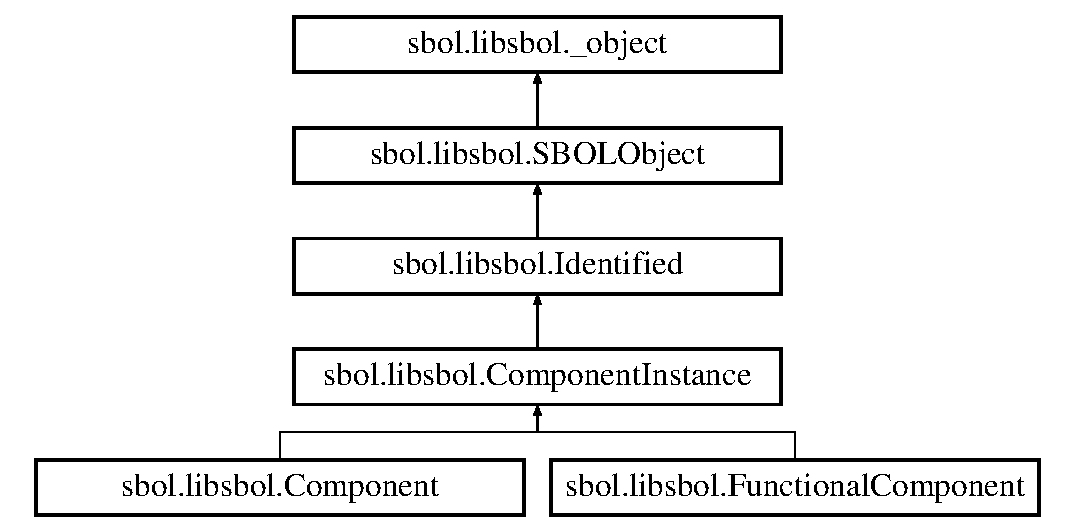
\includegraphics[height=5.000000cm]{classsbol_1_1libsbol_1_1_component_instance}
\end{center}
\end{figure}
\subsection*{Public Member Functions}
\begin{DoxyCompactItemize}
\item 
def {\bfseries \+\_\+\+\_\+init\+\_\+\+\_\+} (self, args, kwargs)\hypertarget{classsbol_1_1libsbol_1_1_component_instance_a2e066b48e3eb405d5ea06ff695381096}{}\label{classsbol_1_1libsbol_1_1_component_instance_a2e066b48e3eb405d5ea06ff695381096}

\end{DoxyCompactItemize}
\subsection*{Static Public Attributes}
\begin{DoxyCompactItemize}
\item 
{\bfseries access} = \+\_\+swig\+\_\+property(\+\_\+libsbol.\+Component\+Instance\+\_\+access\+\_\+get, \+\_\+libsbol.\+Component\+Instance\+\_\+access\+\_\+set)\hypertarget{classsbol_1_1libsbol_1_1_component_instance_a16fa1d797bac6f5e89a0b920cd6986a4}{}\label{classsbol_1_1libsbol_1_1_component_instance_a16fa1d797bac6f5e89a0b920cd6986a4}

\item 
{\bfseries maps\+Tos} = \+\_\+swig\+\_\+property(\+\_\+libsbol.\+Component\+Instance\+\_\+maps\+Tos\+\_\+get, \+\_\+libsbol.\+Component\+Instance\+\_\+maps\+Tos\+\_\+set)\hypertarget{classsbol_1_1libsbol_1_1_component_instance_ad4c4aa7d72960be6e80224714c849e49}{}\label{classsbol_1_1libsbol_1_1_component_instance_ad4c4aa7d72960be6e80224714c849e49}

\item 
{\bfseries definition} = \+\_\+swig\+\_\+property(\+\_\+libsbol.\+Component\+Instance\+\_\+definition\+\_\+get, \+\_\+libsbol.\+Component\+Instance\+\_\+definition\+\_\+set)\hypertarget{classsbol_1_1libsbol_1_1_component_instance_a043086f80356251c30b68b7fc4c34ded}{}\label{classsbol_1_1libsbol_1_1_component_instance_a043086f80356251c30b68b7fc4c34ded}

\end{DoxyCompactItemize}
\subsection*{Additional Inherited Members}


The documentation for this class was generated from the following file\+:\begin{DoxyCompactItemize}
\item 
libsbol.\+py\end{DoxyCompactItemize}

\hypertarget{classsbol_1_1libsbol_1_1_document}{}\section{sbol.\+libsbol.\+Document Class Reference}
\label{classsbol_1_1libsbol_1_1_document}\index{sbol.\+libsbol.\+Document@{sbol.\+libsbol.\+Document}}
Inheritance diagram for sbol.\+libsbol.\+Document\+:\begin{figure}[H]
\begin{center}
\leavevmode
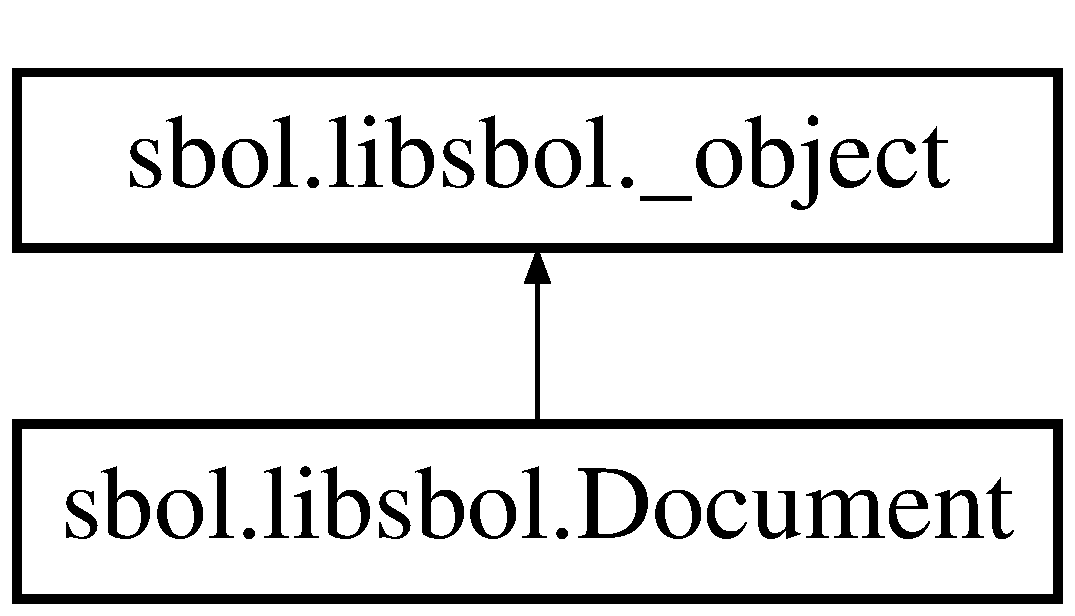
\includegraphics[height=2.000000cm]{classsbol_1_1libsbol_1_1_document}
\end{center}
\end{figure}
\subsection*{Public Member Functions}
\begin{DoxyCompactItemize}
\item 
def \hyperlink{classsbol_1_1libsbol_1_1_document_a63f1fb683227a5f859b4d69c7c112719}{\+\_\+\+\_\+init\+\_\+\+\_\+} (self)
\item 
def \hyperlink{classsbol_1_1libsbol_1_1_document_a7bd75a016d50faabda1a2938a251057f}{get\+Top\+Level} (self, arg2)
\item 
def \hyperlink{classsbol_1_1libsbol_1_1_document_ae578f35d06b76fbb16f671a57122458f}{get\+World} (self)
\item 
def \hyperlink{classsbol_1_1libsbol_1_1_document_a12ad5b7793e9b00a6b776243d1d41c9b}{write} (self, filename)
\item 
def \hyperlink{classsbol_1_1libsbol_1_1_document_aadadbc4e12950cf39ad9abe56f409a01}{read} (self, filename)
\item 
def \hyperlink{classsbol_1_1libsbol_1_1_document_a5dfbca7fef350e3cef714ead3526fdd0}{validate} (self, arg=None)
\item 
def \hyperlink{classsbol_1_1libsbol_1_1_document_a7b0b010ddc545af5edcc52b505d281e8}{get\+Namespaces} (self)
\item 
def \hyperlink{classsbol_1_1libsbol_1_1_document_ae935e1457a5ac794395cecc0103d99fe}{flatten} (self)
\item 
def \hyperlink{classsbol_1_1libsbol_1_1_document_a24148c68a307bd9ed21732b51d7c899c}{add\+Name\+Space} (self, ns, prefix, sbol\+\_\+serializer)
\item 
def \hyperlink{classsbol_1_1libsbol_1_1_document_ae73b90e12d8a22cb4cdef92cf35d9b05}{add\+Component\+Definition} (self, sbol\+\_\+obj)
\item 
def \hyperlink{classsbol_1_1libsbol_1_1_document_a954d9da279c66f9f7208830741ec6f4c}{add\+Sequence} (self, sbol\+\_\+obj)
\item 
def \hyperlink{classsbol_1_1libsbol_1_1_document_ac694a09cc8d745b22f5a8d45ec45e4da}{add\+Model} (self, sbol\+\_\+obj)
\item 
def \hyperlink{classsbol_1_1libsbol_1_1_document_ac1d0d65f573a4ecbacb46d7fd308bfc4}{add\+Module\+Definition} (self, sbol\+\_\+obj)
\item 
def \hyperlink{classsbol_1_1libsbol_1_1_document_a44975d2d2bf308b45b158c14457c9ce2}{get\+Component\+Definition} (self, uri)
\item 
def \hyperlink{classsbol_1_1libsbol_1_1_document_a182f90d0a332c53de4c7696f227a3886}{get\+Sequence} (self, uri)
\item 
def \hyperlink{classsbol_1_1libsbol_1_1_document_af725468fba9d83349617e64513f3d4b4}{get\+Model} (self, uri)
\item 
def \hyperlink{classsbol_1_1libsbol_1_1_document_a4858984056f54cf78830b55c510287ca}{get\+Module\+Definition} (self, uri)
\end{DoxyCompactItemize}
\subsection*{Public Attributes}
\begin{DoxyCompactItemize}
\item 
{\bfseries this}\hypertarget{classsbol_1_1libsbol_1_1_document_a0fa6739ee4f21c6dee56f88538aee3b3}{}\label{classsbol_1_1libsbol_1_1_document_a0fa6739ee4f21c6dee56f88538aee3b3}

\end{DoxyCompactItemize}
\subsection*{Static Public Attributes}
\begin{DoxyCompactItemize}
\item 
{\bfseries S\+B\+O\+L\+Objects} = \+\_\+swig\+\_\+property(\+\_\+libsbol.\+Document\+\_\+\+S\+B\+O\+L\+Objects\+\_\+get, \+\_\+libsbol.\+Document\+\_\+\+S\+B\+O\+L\+Objects\+\_\+set)\hypertarget{classsbol_1_1libsbol_1_1_document_addf1cc5ab6ad90813be3ca2890d3f2c0}{}\label{classsbol_1_1libsbol_1_1_document_addf1cc5ab6ad90813be3ca2890d3f2c0}

\item 
{\bfseries component\+Definitions} = \+\_\+swig\+\_\+property(\+\_\+libsbol.\+Document\+\_\+component\+Definitions\+\_\+get, \+\_\+libsbol.\+Document\+\_\+component\+Definitions\+\_\+set)\hypertarget{classsbol_1_1libsbol_1_1_document_a6209e33914513ccd0c55d4252a0019c4}{}\label{classsbol_1_1libsbol_1_1_document_a6209e33914513ccd0c55d4252a0019c4}

\item 
{\bfseries models} = \+\_\+swig\+\_\+property(\+\_\+libsbol.\+Document\+\_\+models\+\_\+get, \+\_\+libsbol.\+Document\+\_\+models\+\_\+set)\hypertarget{classsbol_1_1libsbol_1_1_document_a856382a0fce02e2ccb04c33c452adc18}{}\label{classsbol_1_1libsbol_1_1_document_a856382a0fce02e2ccb04c33c452adc18}

\item 
{\bfseries module\+Definitions} = \+\_\+swig\+\_\+property(\+\_\+libsbol.\+Document\+\_\+module\+Definitions\+\_\+get, \+\_\+libsbol.\+Document\+\_\+module\+Definitions\+\_\+set)\hypertarget{classsbol_1_1libsbol_1_1_document_aacb86e5f43fb531778eb928d23c72150}{}\label{classsbol_1_1libsbol_1_1_document_aacb86e5f43fb531778eb928d23c72150}

\item 
{\bfseries sequences} = \+\_\+swig\+\_\+property(\+\_\+libsbol.\+Document\+\_\+sequences\+\_\+get, \+\_\+libsbol.\+Document\+\_\+sequences\+\_\+set)\hypertarget{classsbol_1_1libsbol_1_1_document_a6bfc69ce7fac31b5d0140a1eabd23fae}{}\label{classsbol_1_1libsbol_1_1_document_a6bfc69ce7fac31b5d0140a1eabd23fae}

\item 
{\bfseries name\+Spaces} = \+\_\+swig\+\_\+property(\+\_\+libsbol.\+Document\+\_\+name\+Spaces\+\_\+get, \+\_\+libsbol.\+Document\+\_\+name\+Spaces\+\_\+set)\hypertarget{classsbol_1_1libsbol_1_1_document_aacd9264b848f38f76d1ce1993335c8c7}{}\label{classsbol_1_1libsbol_1_1_document_aacd9264b848f38f76d1ce1993335c8c7}

\item 
{\bfseries parse\+\_\+objects} = staticmethod(\+\_\+libsbol.\+Document\+\_\+parse\+\_\+objects)\hypertarget{classsbol_1_1libsbol_1_1_document_ad9fe00e8c9dab72eed42c9e57ef05ad0}{}\label{classsbol_1_1libsbol_1_1_document_ad9fe00e8c9dab72eed42c9e57ef05ad0}

\item 
{\bfseries parse\+\_\+properties} = staticmethod(\+\_\+libsbol.\+Document\+\_\+parse\+\_\+properties)\hypertarget{classsbol_1_1libsbol_1_1_document_af1be03e32077c89cec540b16c890eddf}{}\label{classsbol_1_1libsbol_1_1_document_af1be03e32077c89cec540b16c890eddf}

\item 
{\bfseries namespace\+Handler} = staticmethod(\+\_\+libsbol.\+Document\+\_\+namespace\+Handler)\hypertarget{classsbol_1_1libsbol_1_1_document_a30a2303398162f5df252afc155fbd517}{}\label{classsbol_1_1libsbol_1_1_document_a30a2303398162f5df252afc155fbd517}

\end{DoxyCompactItemize}


\subsection{Detailed Description}
\begin{DoxyVerb}Read and write SBOL using a Document class. The Document is a
container for Components, Modules, and all other SBOLObjects.

C++ includes: document.h 
\end{DoxyVerb}
 

\subsection{Constructor \& Destructor Documentation}
\index{sbol\+::libsbol\+::\+Document@{sbol\+::libsbol\+::\+Document}!\+\_\+\+\_\+init\+\_\+\+\_\+@{\+\_\+\+\_\+init\+\_\+\+\_\+}}
\index{\+\_\+\+\_\+init\+\_\+\+\_\+@{\+\_\+\+\_\+init\+\_\+\+\_\+}!sbol\+::libsbol\+::\+Document@{sbol\+::libsbol\+::\+Document}}
\subsubsection[{\texorpdfstring{\+\_\+\+\_\+init\+\_\+\+\_\+(self)}{__init__(self)}}]{\setlength{\rightskip}{0pt plus 5cm}def sbol.\+libsbol.\+Document.\+\_\+\+\_\+init\+\_\+\+\_\+ (
\begin{DoxyParamCaption}
\item[{}]{self}
\end{DoxyParamCaption}
)}\hypertarget{classsbol_1_1libsbol_1_1_document_a63f1fb683227a5f859b4d69c7c112719}{}\label{classsbol_1_1libsbol_1_1_document_a63f1fb683227a5f859b4d69c7c112719}
\begin{DoxyVerb}sbol::Document::Document() \end{DoxyVerb}
 

\subsection{Member Function Documentation}
\index{sbol\+::libsbol\+::\+Document@{sbol\+::libsbol\+::\+Document}!add\+Component\+Definition@{add\+Component\+Definition}}
\index{add\+Component\+Definition@{add\+Component\+Definition}!sbol\+::libsbol\+::\+Document@{sbol\+::libsbol\+::\+Document}}
\subsubsection[{\texorpdfstring{add\+Component\+Definition(self, sbol\+\_\+obj)}{addComponentDefinition(self, sbol_obj)}}]{\setlength{\rightskip}{0pt plus 5cm}def sbol.\+libsbol.\+Document.\+add\+Component\+Definition (
\begin{DoxyParamCaption}
\item[{}]{self, }
\item[{}]{sbol\+\_\+obj}
\end{DoxyParamCaption}
)}\hypertarget{classsbol_1_1libsbol_1_1_document_ae73b90e12d8a22cb4cdef92cf35d9b05}{}\label{classsbol_1_1libsbol_1_1_document_ae73b90e12d8a22cb4cdef92cf35d9b05}
\begin{DoxyVerb}void
sbol::Document::add(SBOLClass &sbol_obj) 
\end{DoxyVerb}
 \index{sbol\+::libsbol\+::\+Document@{sbol\+::libsbol\+::\+Document}!add\+Model@{add\+Model}}
\index{add\+Model@{add\+Model}!sbol\+::libsbol\+::\+Document@{sbol\+::libsbol\+::\+Document}}
\subsubsection[{\texorpdfstring{add\+Model(self, sbol\+\_\+obj)}{addModel(self, sbol_obj)}}]{\setlength{\rightskip}{0pt plus 5cm}def sbol.\+libsbol.\+Document.\+add\+Model (
\begin{DoxyParamCaption}
\item[{}]{self, }
\item[{}]{sbol\+\_\+obj}
\end{DoxyParamCaption}
)}\hypertarget{classsbol_1_1libsbol_1_1_document_ac694a09cc8d745b22f5a8d45ec45e4da}{}\label{classsbol_1_1libsbol_1_1_document_ac694a09cc8d745b22f5a8d45ec45e4da}
\begin{DoxyVerb}void
sbol::Document::add(SBOLClass &sbol_obj) 
\end{DoxyVerb}
 \index{sbol\+::libsbol\+::\+Document@{sbol\+::libsbol\+::\+Document}!add\+Module\+Definition@{add\+Module\+Definition}}
\index{add\+Module\+Definition@{add\+Module\+Definition}!sbol\+::libsbol\+::\+Document@{sbol\+::libsbol\+::\+Document}}
\subsubsection[{\texorpdfstring{add\+Module\+Definition(self, sbol\+\_\+obj)}{addModuleDefinition(self, sbol_obj)}}]{\setlength{\rightskip}{0pt plus 5cm}def sbol.\+libsbol.\+Document.\+add\+Module\+Definition (
\begin{DoxyParamCaption}
\item[{}]{self, }
\item[{}]{sbol\+\_\+obj}
\end{DoxyParamCaption}
)}\hypertarget{classsbol_1_1libsbol_1_1_document_ac1d0d65f573a4ecbacb46d7fd308bfc4}{}\label{classsbol_1_1libsbol_1_1_document_ac1d0d65f573a4ecbacb46d7fd308bfc4}
\begin{DoxyVerb}void
sbol::Document::add(SBOLClass &sbol_obj) 
\end{DoxyVerb}
 \index{sbol\+::libsbol\+::\+Document@{sbol\+::libsbol\+::\+Document}!add\+Name\+Space@{add\+Name\+Space}}
\index{add\+Name\+Space@{add\+Name\+Space}!sbol\+::libsbol\+::\+Document@{sbol\+::libsbol\+::\+Document}}
\subsubsection[{\texorpdfstring{add\+Name\+Space(self, ns, prefix, sbol\+\_\+serializer)}{addNameSpace(self, ns, prefix, sbol_serializer)}}]{\setlength{\rightskip}{0pt plus 5cm}def sbol.\+libsbol.\+Document.\+add\+Name\+Space (
\begin{DoxyParamCaption}
\item[{}]{self, }
\item[{}]{ns, }
\item[{}]{prefix, }
\item[{}]{sbol\+\_\+serializer}
\end{DoxyParamCaption}
)}\hypertarget{classsbol_1_1libsbol_1_1_document_a24148c68a307bd9ed21732b51d7c899c}{}\label{classsbol_1_1libsbol_1_1_document_a24148c68a307bd9ed21732b51d7c899c}
\begin{DoxyVerb}void
sbol::Document::addNameSpace(std::string ns, std::string prefix,
raptor_serializer *sbol_serializer) 
\end{DoxyVerb}
 \index{sbol\+::libsbol\+::\+Document@{sbol\+::libsbol\+::\+Document}!add\+Sequence@{add\+Sequence}}
\index{add\+Sequence@{add\+Sequence}!sbol\+::libsbol\+::\+Document@{sbol\+::libsbol\+::\+Document}}
\subsubsection[{\texorpdfstring{add\+Sequence(self, sbol\+\_\+obj)}{addSequence(self, sbol_obj)}}]{\setlength{\rightskip}{0pt plus 5cm}def sbol.\+libsbol.\+Document.\+add\+Sequence (
\begin{DoxyParamCaption}
\item[{}]{self, }
\item[{}]{sbol\+\_\+obj}
\end{DoxyParamCaption}
)}\hypertarget{classsbol_1_1libsbol_1_1_document_a954d9da279c66f9f7208830741ec6f4c}{}\label{classsbol_1_1libsbol_1_1_document_a954d9da279c66f9f7208830741ec6f4c}
\begin{DoxyVerb}void
sbol::Document::add(SBOLClass &sbol_obj) 
\end{DoxyVerb}
 \index{sbol\+::libsbol\+::\+Document@{sbol\+::libsbol\+::\+Document}!flatten@{flatten}}
\index{flatten@{flatten}!sbol\+::libsbol\+::\+Document@{sbol\+::libsbol\+::\+Document}}
\subsubsection[{\texorpdfstring{flatten(self)}{flatten(self)}}]{\setlength{\rightskip}{0pt plus 5cm}def sbol.\+libsbol.\+Document.\+flatten (
\begin{DoxyParamCaption}
\item[{}]{self}
\end{DoxyParamCaption}
)}\hypertarget{classsbol_1_1libsbol_1_1_document_ae935e1457a5ac794395cecc0103d99fe}{}\label{classsbol_1_1libsbol_1_1_document_ae935e1457a5ac794395cecc0103d99fe}
\begin{DoxyVerb}std::vector<SBOLObject*> sbol::Document::flatten() \end{DoxyVerb}
 \index{sbol\+::libsbol\+::\+Document@{sbol\+::libsbol\+::\+Document}!get\+Component\+Definition@{get\+Component\+Definition}}
\index{get\+Component\+Definition@{get\+Component\+Definition}!sbol\+::libsbol\+::\+Document@{sbol\+::libsbol\+::\+Document}}
\subsubsection[{\texorpdfstring{get\+Component\+Definition(self, uri)}{getComponentDefinition(self, uri)}}]{\setlength{\rightskip}{0pt plus 5cm}def sbol.\+libsbol.\+Document.\+get\+Component\+Definition (
\begin{DoxyParamCaption}
\item[{}]{self, }
\item[{}]{uri}
\end{DoxyParamCaption}
)}\hypertarget{classsbol_1_1libsbol_1_1_document_a44975d2d2bf308b45b158c14457c9ce2}{}\label{classsbol_1_1libsbol_1_1_document_a44975d2d2bf308b45b158c14457c9ce2}
\begin{DoxyVerb}SBOLClass &
sbol::Document::get(std::string uri) 
\end{DoxyVerb}
 \index{sbol\+::libsbol\+::\+Document@{sbol\+::libsbol\+::\+Document}!get\+Model@{get\+Model}}
\index{get\+Model@{get\+Model}!sbol\+::libsbol\+::\+Document@{sbol\+::libsbol\+::\+Document}}
\subsubsection[{\texorpdfstring{get\+Model(self, uri)}{getModel(self, uri)}}]{\setlength{\rightskip}{0pt plus 5cm}def sbol.\+libsbol.\+Document.\+get\+Model (
\begin{DoxyParamCaption}
\item[{}]{self, }
\item[{}]{uri}
\end{DoxyParamCaption}
)}\hypertarget{classsbol_1_1libsbol_1_1_document_af725468fba9d83349617e64513f3d4b4}{}\label{classsbol_1_1libsbol_1_1_document_af725468fba9d83349617e64513f3d4b4}
\begin{DoxyVerb}SBOLClass &
sbol::Document::get(std::string uri) 
\end{DoxyVerb}
 \index{sbol\+::libsbol\+::\+Document@{sbol\+::libsbol\+::\+Document}!get\+Module\+Definition@{get\+Module\+Definition}}
\index{get\+Module\+Definition@{get\+Module\+Definition}!sbol\+::libsbol\+::\+Document@{sbol\+::libsbol\+::\+Document}}
\subsubsection[{\texorpdfstring{get\+Module\+Definition(self, uri)}{getModuleDefinition(self, uri)}}]{\setlength{\rightskip}{0pt plus 5cm}def sbol.\+libsbol.\+Document.\+get\+Module\+Definition (
\begin{DoxyParamCaption}
\item[{}]{self, }
\item[{}]{uri}
\end{DoxyParamCaption}
)}\hypertarget{classsbol_1_1libsbol_1_1_document_a4858984056f54cf78830b55c510287ca}{}\label{classsbol_1_1libsbol_1_1_document_a4858984056f54cf78830b55c510287ca}
\begin{DoxyVerb}SBOLClass &
sbol::Document::get(std::string uri) 
\end{DoxyVerb}
 \index{sbol\+::libsbol\+::\+Document@{sbol\+::libsbol\+::\+Document}!get\+Namespaces@{get\+Namespaces}}
\index{get\+Namespaces@{get\+Namespaces}!sbol\+::libsbol\+::\+Document@{sbol\+::libsbol\+::\+Document}}
\subsubsection[{\texorpdfstring{get\+Namespaces(self)}{getNamespaces(self)}}]{\setlength{\rightskip}{0pt plus 5cm}def sbol.\+libsbol.\+Document.\+get\+Namespaces (
\begin{DoxyParamCaption}
\item[{}]{self}
\end{DoxyParamCaption}
)}\hypertarget{classsbol_1_1libsbol_1_1_document_a7b0b010ddc545af5edcc52b505d281e8}{}\label{classsbol_1_1libsbol_1_1_document_a7b0b010ddc545af5edcc52b505d281e8}
\begin{DoxyVerb}std::vector<std::string> sbol::Document::getNamespaces() \end{DoxyVerb}
 \index{sbol\+::libsbol\+::\+Document@{sbol\+::libsbol\+::\+Document}!get\+Sequence@{get\+Sequence}}
\index{get\+Sequence@{get\+Sequence}!sbol\+::libsbol\+::\+Document@{sbol\+::libsbol\+::\+Document}}
\subsubsection[{\texorpdfstring{get\+Sequence(self, uri)}{getSequence(self, uri)}}]{\setlength{\rightskip}{0pt plus 5cm}def sbol.\+libsbol.\+Document.\+get\+Sequence (
\begin{DoxyParamCaption}
\item[{}]{self, }
\item[{}]{uri}
\end{DoxyParamCaption}
)}\hypertarget{classsbol_1_1libsbol_1_1_document_a182f90d0a332c53de4c7696f227a3886}{}\label{classsbol_1_1libsbol_1_1_document_a182f90d0a332c53de4c7696f227a3886}
\begin{DoxyVerb}SBOLClass &
sbol::Document::get(std::string uri) 
\end{DoxyVerb}
 \index{sbol\+::libsbol\+::\+Document@{sbol\+::libsbol\+::\+Document}!get\+Top\+Level@{get\+Top\+Level}}
\index{get\+Top\+Level@{get\+Top\+Level}!sbol\+::libsbol\+::\+Document@{sbol\+::libsbol\+::\+Document}}
\subsubsection[{\texorpdfstring{get\+Top\+Level(self, arg2)}{getTopLevel(self, arg2)}}]{\setlength{\rightskip}{0pt plus 5cm}def sbol.\+libsbol.\+Document.\+get\+Top\+Level (
\begin{DoxyParamCaption}
\item[{}]{self, }
\item[{}]{arg2}
\end{DoxyParamCaption}
)}\hypertarget{classsbol_1_1libsbol_1_1_document_a7bd75a016d50faabda1a2938a251057f}{}\label{classsbol_1_1libsbol_1_1_document_a7bd75a016d50faabda1a2938a251057f}
\begin{DoxyVerb}TopLevel&
sbol::Document::getTopLevel(std::string) 
\end{DoxyVerb}
 \index{sbol\+::libsbol\+::\+Document@{sbol\+::libsbol\+::\+Document}!get\+World@{get\+World}}
\index{get\+World@{get\+World}!sbol\+::libsbol\+::\+Document@{sbol\+::libsbol\+::\+Document}}
\subsubsection[{\texorpdfstring{get\+World(self)}{getWorld(self)}}]{\setlength{\rightskip}{0pt plus 5cm}def sbol.\+libsbol.\+Document.\+get\+World (
\begin{DoxyParamCaption}
\item[{}]{self}
\end{DoxyParamCaption}
)}\hypertarget{classsbol_1_1libsbol_1_1_document_ae578f35d06b76fbb16f671a57122458f}{}\label{classsbol_1_1libsbol_1_1_document_ae578f35d06b76fbb16f671a57122458f}
\begin{DoxyVerb}raptor_world*
sbol::Document::getWorld() 
\end{DoxyVerb}
 \index{sbol\+::libsbol\+::\+Document@{sbol\+::libsbol\+::\+Document}!read@{read}}
\index{read@{read}!sbol\+::libsbol\+::\+Document@{sbol\+::libsbol\+::\+Document}}
\subsubsection[{\texorpdfstring{read(self, filename)}{read(self, filename)}}]{\setlength{\rightskip}{0pt plus 5cm}def sbol.\+libsbol.\+Document.\+read (
\begin{DoxyParamCaption}
\item[{}]{self, }
\item[{}]{filename}
\end{DoxyParamCaption}
)}\hypertarget{classsbol_1_1libsbol_1_1_document_aadadbc4e12950cf39ad9abe56f409a01}{}\label{classsbol_1_1libsbol_1_1_document_aadadbc4e12950cf39ad9abe56f409a01}
\begin{DoxyVerb}void
sbol::Document::read(std::string filename) 
\end{DoxyVerb}
 \index{sbol\+::libsbol\+::\+Document@{sbol\+::libsbol\+::\+Document}!validate@{validate}}
\index{validate@{validate}!sbol\+::libsbol\+::\+Document@{sbol\+::libsbol\+::\+Document}}
\subsubsection[{\texorpdfstring{validate(self, arg=\+None)}{validate(self, arg=None)}}]{\setlength{\rightskip}{0pt plus 5cm}def sbol.\+libsbol.\+Document.\+validate (
\begin{DoxyParamCaption}
\item[{}]{self, }
\item[{}]{arg = {\ttfamily None}}
\end{DoxyParamCaption}
)}\hypertarget{classsbol_1_1libsbol_1_1_document_a5dfbca7fef350e3cef714ead3526fdd0}{}\label{classsbol_1_1libsbol_1_1_document_a5dfbca7fef350e3cef714ead3526fdd0}
\begin{DoxyVerb}void
sbol::Document::validate(void *arg=NULL) 
\end{DoxyVerb}
 \index{sbol\+::libsbol\+::\+Document@{sbol\+::libsbol\+::\+Document}!write@{write}}
\index{write@{write}!sbol\+::libsbol\+::\+Document@{sbol\+::libsbol\+::\+Document}}
\subsubsection[{\texorpdfstring{write(self, filename)}{write(self, filename)}}]{\setlength{\rightskip}{0pt plus 5cm}def sbol.\+libsbol.\+Document.\+write (
\begin{DoxyParamCaption}
\item[{}]{self, }
\item[{}]{filename}
\end{DoxyParamCaption}
)}\hypertarget{classsbol_1_1libsbol_1_1_document_a12ad5b7793e9b00a6b776243d1d41c9b}{}\label{classsbol_1_1libsbol_1_1_document_a12ad5b7793e9b00a6b776243d1d41c9b}
\begin{DoxyVerb}void
sbol::Document::write(std::string filename) 
\end{DoxyVerb}
 

The documentation for this class was generated from the following file\+:\begin{DoxyCompactItemize}
\item 
libsbol.\+py\end{DoxyCompactItemize}

\hypertarget{classsbol_1_1libsbol_1_1_functional_component}{}\section{sbol.\+libsbol.\+Functional\+Component Class Reference}
\label{classsbol_1_1libsbol_1_1_functional_component}\index{sbol.\+libsbol.\+Functional\+Component@{sbol.\+libsbol.\+Functional\+Component}}
Inheritance diagram for sbol.\+libsbol.\+Functional\+Component\+:\begin{figure}[H]
\begin{center}
\leavevmode
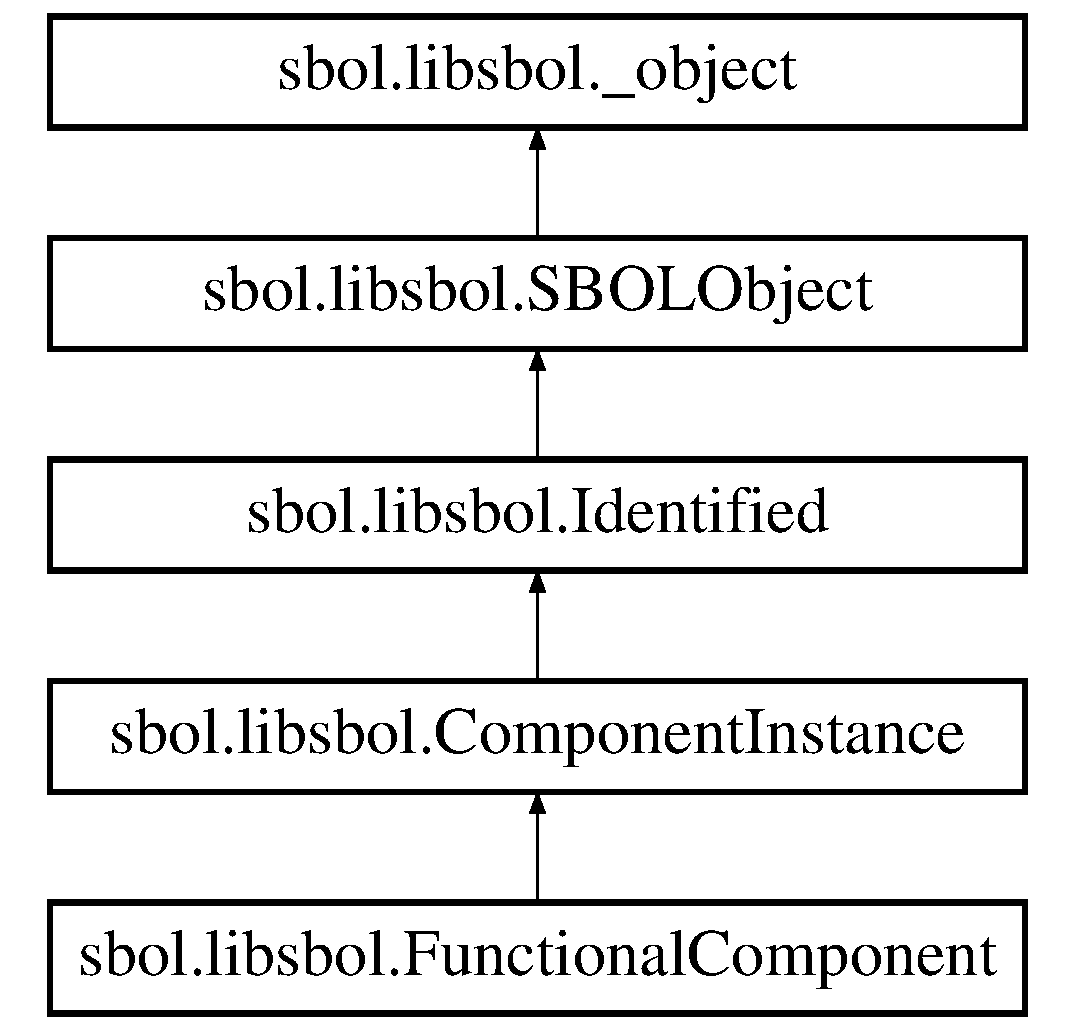
\includegraphics[height=5.000000cm]{classsbol_1_1libsbol_1_1_functional_component}
\end{center}
\end{figure}
\subsection*{Public Member Functions}
\begin{DoxyCompactItemize}
\item 
def \hyperlink{classsbol_1_1libsbol_1_1_functional_component_a8d77872e0dc59dc4de54f88ab09d6cb3}{\+\_\+\+\_\+init\+\_\+\+\_\+} (self, args)
\end{DoxyCompactItemize}
\subsection*{Public Attributes}
\begin{DoxyCompactItemize}
\item 
{\bfseries this}\hypertarget{classsbol_1_1libsbol_1_1_functional_component_af54267278905312669110963b9bf0a99}{}\label{classsbol_1_1libsbol_1_1_functional_component_af54267278905312669110963b9bf0a99}

\end{DoxyCompactItemize}
\subsection*{Static Public Attributes}
\begin{DoxyCompactItemize}
\item 
{\bfseries direction} = \+\_\+swig\+\_\+property(\+\_\+libsbol.\+Functional\+Component\+\_\+direction\+\_\+get, \+\_\+libsbol.\+Functional\+Component\+\_\+direction\+\_\+set)\hypertarget{classsbol_1_1libsbol_1_1_functional_component_a2b9f016242b2ef44ab32b604df86d179}{}\label{classsbol_1_1libsbol_1_1_functional_component_a2b9f016242b2ef44ab32b604df86d179}

\end{DoxyCompactItemize}


\subsection{Constructor \& Destructor Documentation}
\index{sbol\+::libsbol\+::\+Functional\+Component@{sbol\+::libsbol\+::\+Functional\+Component}!\+\_\+\+\_\+init\+\_\+\+\_\+@{\+\_\+\+\_\+init\+\_\+\+\_\+}}
\index{\+\_\+\+\_\+init\+\_\+\+\_\+@{\+\_\+\+\_\+init\+\_\+\+\_\+}!sbol\+::libsbol\+::\+Functional\+Component@{sbol\+::libsbol\+::\+Functional\+Component}}
\subsubsection[{\texorpdfstring{\+\_\+\+\_\+init\+\_\+\+\_\+(self, args)}{__init__(self, args)}}]{\setlength{\rightskip}{0pt plus 5cm}def sbol.\+libsbol.\+Functional\+Component.\+\_\+\+\_\+init\+\_\+\+\_\+ (
\begin{DoxyParamCaption}
\item[{}]{self, }
\item[{}]{args}
\end{DoxyParamCaption}
)}\hypertarget{classsbol_1_1libsbol_1_1_functional_component_a8d77872e0dc59dc4de54f88ab09d6cb3}{}\label{classsbol_1_1libsbol_1_1_functional_component_a8d77872e0dc59dc4de54f88ab09d6cb3}
\begin{DoxyVerb}sbol::FunctionalComponent::FunctionalComponent(std::string
uri_prefix, std::string display_id, std::string version, std::string
definition, std::string access, std::string direction) 
\end{DoxyVerb}
 

The documentation for this class was generated from the following file\+:\begin{DoxyCompactItemize}
\item 
libsbol.\+py\end{DoxyCompactItemize}

\hypertarget{classsbol_1_1libsbol_1_1functional_component_property}{}\section{sbol.\+libsbol.\+functional\+Component\+Property Class Reference}
\label{classsbol_1_1libsbol_1_1functional_component_property}\index{sbol.\+libsbol.\+functional\+Component\+Property@{sbol.\+libsbol.\+functional\+Component\+Property}}
Inheritance diagram for sbol.\+libsbol.\+functional\+Component\+Property\+:\begin{figure}[H]
\begin{center}
\leavevmode
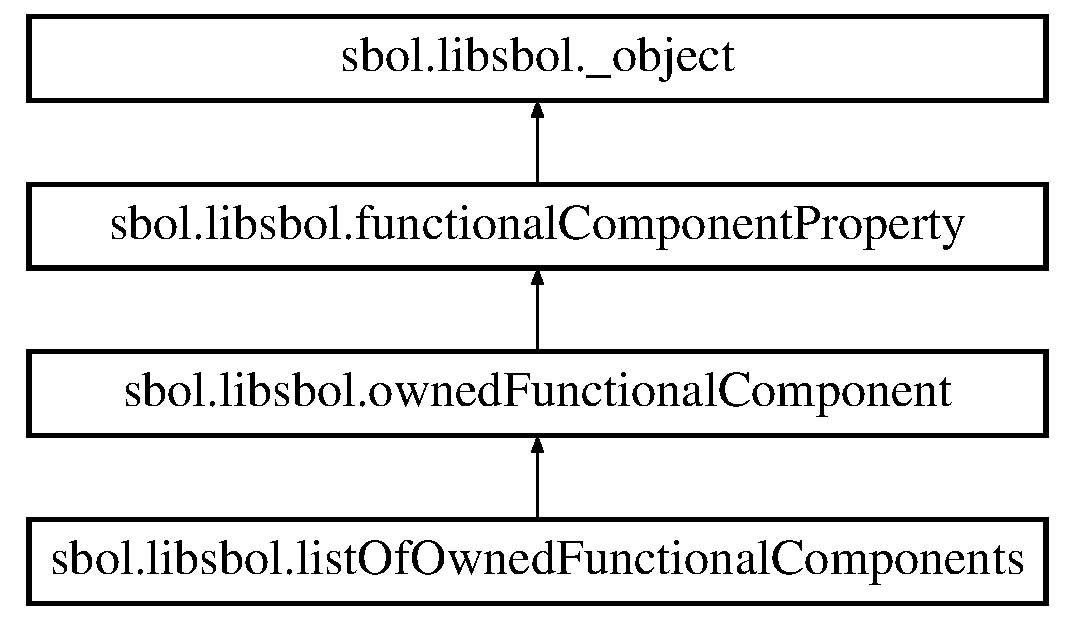
\includegraphics[height=4.000000cm]{classsbol_1_1libsbol_1_1functional_component_property}
\end{center}
\end{figure}
\subsection*{Public Member Functions}
\begin{DoxyCompactItemize}
\item 
def \hyperlink{classsbol_1_1libsbol_1_1functional_component_property_a1d475379fddfbf218a04c2714d28f9ea}{\+\_\+\+\_\+init\+\_\+\+\_\+} (self, args)
\item 
def \hyperlink{classsbol_1_1libsbol_1_1functional_component_property_aec805b412d217695cbe26ea9913029ad}{get\+Type\+U\+RI} (self)
\item 
def \hyperlink{classsbol_1_1libsbol_1_1functional_component_property_a5f1aad9330199a53461ad477da1a96f7}{get\+Owner} (self)
\item 
def \hyperlink{classsbol_1_1libsbol_1_1functional_component_property_abd22c36e0be47420ac27aadd8c92b5ad}{get} (self)
\item 
def \hyperlink{classsbol_1_1libsbol_1_1functional_component_property_a0a283df8430befc7f1874094af815c29}{add} (self, new\+\_\+value)
\item 
def \hyperlink{classsbol_1_1libsbol_1_1functional_component_property_affc5dce5d9c542e81ab8948b17f59a38}{set} (self, args)
\item 
def \hyperlink{classsbol_1_1libsbol_1_1functional_component_property_aef2523491122d152a37ef4094def9dbe}{write} (self)
\item 
def \hyperlink{classsbol_1_1libsbol_1_1functional_component_property_a8e66c9b34d2e98f02c01b25ec9973579}{validate} (self, arg=None)
\item 
def {\bfseries \+\_\+\+\_\+getitem\+\_\+\+\_\+} (self, n\+Index)\hypertarget{classsbol_1_1libsbol_1_1functional_component_property_a15c50beaec5957b8cabf72a04b636c3c}{}\label{classsbol_1_1libsbol_1_1functional_component_property_a15c50beaec5957b8cabf72a04b636c3c}

\item 
def {\bfseries \+\_\+\+\_\+iter\+\_\+\+\_\+} (self)\hypertarget{classsbol_1_1libsbol_1_1functional_component_property_a10cb12912fe030f3e638466deaf27d62}{}\label{classsbol_1_1libsbol_1_1functional_component_property_a10cb12912fe030f3e638466deaf27d62}

\item 
def {\bfseries next} (self)\hypertarget{classsbol_1_1libsbol_1_1functional_component_property_aeea82def56975c24afee110d9d0bb3e2}{}\label{classsbol_1_1libsbol_1_1functional_component_property_aeea82def56975c24afee110d9d0bb3e2}

\item 
def {\bfseries \+\_\+\+\_\+len\+\_\+\+\_\+} (self)\hypertarget{classsbol_1_1libsbol_1_1functional_component_property_ae772bec611c404f5b11b5a2b44d6bea7}{}\label{classsbol_1_1libsbol_1_1functional_component_property_ae772bec611c404f5b11b5a2b44d6bea7}

\end{DoxyCompactItemize}
\subsection*{Public Attributes}
\begin{DoxyCompactItemize}
\item 
{\bfseries this}\hypertarget{classsbol_1_1libsbol_1_1functional_component_property_a8cabb3ceb81dcf1583051f0a7adc18fb}{}\label{classsbol_1_1libsbol_1_1functional_component_property_a8cabb3ceb81dcf1583051f0a7adc18fb}

\end{DoxyCompactItemize}


\subsection{Detailed Description}
\begin{DoxyVerb}metafunction for generation of a map of message types to their
associated callbacks.

Usage: Use generate_callback_map<Type>::type to ...

Parameters:
-----------

LiteralType:  The library currently supports Property<string> and
Property<int> specification currently supports integer, string, and
URI literals

C++ includes: property.h 
\end{DoxyVerb}
 

\subsection{Constructor \& Destructor Documentation}
\index{sbol\+::libsbol\+::functional\+Component\+Property@{sbol\+::libsbol\+::functional\+Component\+Property}!\+\_\+\+\_\+init\+\_\+\+\_\+@{\+\_\+\+\_\+init\+\_\+\+\_\+}}
\index{\+\_\+\+\_\+init\+\_\+\+\_\+@{\+\_\+\+\_\+init\+\_\+\+\_\+}!sbol\+::libsbol\+::functional\+Component\+Property@{sbol\+::libsbol\+::functional\+Component\+Property}}
\subsubsection[{\texorpdfstring{\+\_\+\+\_\+init\+\_\+\+\_\+(self, args)}{__init__(self, args)}}]{\setlength{\rightskip}{0pt plus 5cm}def sbol.\+libsbol.\+functional\+Component\+Property.\+\_\+\+\_\+init\+\_\+\+\_\+ (
\begin{DoxyParamCaption}
\item[{}]{self, }
\item[{}]{args}
\end{DoxyParamCaption}
)}\hypertarget{classsbol_1_1libsbol_1_1functional_component_property_a1d475379fddfbf218a04c2714d28f9ea}{}\label{classsbol_1_1libsbol_1_1functional_component_property_a1d475379fddfbf218a04c2714d28f9ea}
\begin{DoxyVerb}sbol::Property<
LiteralType >::Property(sbol_type type_uri=UNDEFINED, void
*property_owner=NULL, ValidationRules validation_rules={}) 
\end{DoxyVerb}
 

\subsection{Member Function Documentation}
\index{sbol\+::libsbol\+::functional\+Component\+Property@{sbol\+::libsbol\+::functional\+Component\+Property}!add@{add}}
\index{add@{add}!sbol\+::libsbol\+::functional\+Component\+Property@{sbol\+::libsbol\+::functional\+Component\+Property}}
\subsubsection[{\texorpdfstring{add(self, new\+\_\+value)}{add(self, new_value)}}]{\setlength{\rightskip}{0pt plus 5cm}def sbol.\+libsbol.\+functional\+Component\+Property.\+add (
\begin{DoxyParamCaption}
\item[{}]{self, }
\item[{}]{new\+\_\+value}
\end{DoxyParamCaption}
)}\hypertarget{classsbol_1_1libsbol_1_1functional_component_property_a0a283df8430befc7f1874094af815c29}{}\label{classsbol_1_1libsbol_1_1functional_component_property_a0a283df8430befc7f1874094af815c29}
\begin{DoxyVerb}void sbol::Property<
LiteralType >::add(std::string new_value) 
\end{DoxyVerb}
 \index{sbol\+::libsbol\+::functional\+Component\+Property@{sbol\+::libsbol\+::functional\+Component\+Property}!get@{get}}
\index{get@{get}!sbol\+::libsbol\+::functional\+Component\+Property@{sbol\+::libsbol\+::functional\+Component\+Property}}
\subsubsection[{\texorpdfstring{get(self)}{get(self)}}]{\setlength{\rightskip}{0pt plus 5cm}def sbol.\+libsbol.\+functional\+Component\+Property.\+get (
\begin{DoxyParamCaption}
\item[{}]{self}
\end{DoxyParamCaption}
)}\hypertarget{classsbol_1_1libsbol_1_1functional_component_property_abd22c36e0be47420ac27aadd8c92b5ad}{}\label{classsbol_1_1libsbol_1_1functional_component_property_abd22c36e0be47420ac27aadd8c92b5ad}
\begin{DoxyVerb}std::string
sbol::Property< LiteralType >::get() 
\end{DoxyVerb}
 \index{sbol\+::libsbol\+::functional\+Component\+Property@{sbol\+::libsbol\+::functional\+Component\+Property}!get\+Owner@{get\+Owner}}
\index{get\+Owner@{get\+Owner}!sbol\+::libsbol\+::functional\+Component\+Property@{sbol\+::libsbol\+::functional\+Component\+Property}}
\subsubsection[{\texorpdfstring{get\+Owner(self)}{getOwner(self)}}]{\setlength{\rightskip}{0pt plus 5cm}def sbol.\+libsbol.\+functional\+Component\+Property.\+get\+Owner (
\begin{DoxyParamCaption}
\item[{}]{self}
\end{DoxyParamCaption}
)}\hypertarget{classsbol_1_1libsbol_1_1functional_component_property_a5f1aad9330199a53461ad477da1a96f7}{}\label{classsbol_1_1libsbol_1_1functional_component_property_a5f1aad9330199a53461ad477da1a96f7}
\begin{DoxyVerb}SBOLObject &
sbol::Property< LiteralType >::getOwner() 
\end{DoxyVerb}
 \index{sbol\+::libsbol\+::functional\+Component\+Property@{sbol\+::libsbol\+::functional\+Component\+Property}!get\+Type\+U\+RI@{get\+Type\+U\+RI}}
\index{get\+Type\+U\+RI@{get\+Type\+U\+RI}!sbol\+::libsbol\+::functional\+Component\+Property@{sbol\+::libsbol\+::functional\+Component\+Property}}
\subsubsection[{\texorpdfstring{get\+Type\+U\+R\+I(self)}{getTypeURI(self)}}]{\setlength{\rightskip}{0pt plus 5cm}def sbol.\+libsbol.\+functional\+Component\+Property.\+get\+Type\+U\+RI (
\begin{DoxyParamCaption}
\item[{}]{self}
\end{DoxyParamCaption}
)}\hypertarget{classsbol_1_1libsbol_1_1functional_component_property_aec805b412d217695cbe26ea9913029ad}{}\label{classsbol_1_1libsbol_1_1functional_component_property_aec805b412d217695cbe26ea9913029ad}
\begin{DoxyVerb}sbol_type
sbol::Property< LiteralType >::getTypeURI() 
\end{DoxyVerb}
 \index{sbol\+::libsbol\+::functional\+Component\+Property@{sbol\+::libsbol\+::functional\+Component\+Property}!set@{set}}
\index{set@{set}!sbol\+::libsbol\+::functional\+Component\+Property@{sbol\+::libsbol\+::functional\+Component\+Property}}
\subsubsection[{\texorpdfstring{set(self, args)}{set(self, args)}}]{\setlength{\rightskip}{0pt plus 5cm}def sbol.\+libsbol.\+functional\+Component\+Property.\+set (
\begin{DoxyParamCaption}
\item[{}]{self, }
\item[{}]{args}
\end{DoxyParamCaption}
)}\hypertarget{classsbol_1_1libsbol_1_1functional_component_property_affc5dce5d9c542e81ab8948b17f59a38}{}\label{classsbol_1_1libsbol_1_1functional_component_property_affc5dce5d9c542e81ab8948b17f59a38}
\begin{DoxyVerb}void sbol::Property<
LiteralType >::set(int new_value) 
\end{DoxyVerb}
 \index{sbol\+::libsbol\+::functional\+Component\+Property@{sbol\+::libsbol\+::functional\+Component\+Property}!validate@{validate}}
\index{validate@{validate}!sbol\+::libsbol\+::functional\+Component\+Property@{sbol\+::libsbol\+::functional\+Component\+Property}}
\subsubsection[{\texorpdfstring{validate(self, arg=\+None)}{validate(self, arg=None)}}]{\setlength{\rightskip}{0pt plus 5cm}def sbol.\+libsbol.\+functional\+Component\+Property.\+validate (
\begin{DoxyParamCaption}
\item[{}]{self, }
\item[{}]{arg = {\ttfamily None}}
\end{DoxyParamCaption}
)}\hypertarget{classsbol_1_1libsbol_1_1functional_component_property_a8e66c9b34d2e98f02c01b25ec9973579}{}\label{classsbol_1_1libsbol_1_1functional_component_property_a8e66c9b34d2e98f02c01b25ec9973579}
\begin{DoxyVerb}void sbol::Property<
LiteralType >::validate(void *arg=NULL) 
\end{DoxyVerb}
 \index{sbol\+::libsbol\+::functional\+Component\+Property@{sbol\+::libsbol\+::functional\+Component\+Property}!write@{write}}
\index{write@{write}!sbol\+::libsbol\+::functional\+Component\+Property@{sbol\+::libsbol\+::functional\+Component\+Property}}
\subsubsection[{\texorpdfstring{write(self)}{write(self)}}]{\setlength{\rightskip}{0pt plus 5cm}def sbol.\+libsbol.\+functional\+Component\+Property.\+write (
\begin{DoxyParamCaption}
\item[{}]{self}
\end{DoxyParamCaption}
)}\hypertarget{classsbol_1_1libsbol_1_1functional_component_property_aef2523491122d152a37ef4094def9dbe}{}\label{classsbol_1_1libsbol_1_1functional_component_property_aef2523491122d152a37ef4094def9dbe}
\begin{DoxyVerb}void sbol::Property<
LiteralType >::write() 
\end{DoxyVerb}
 

The documentation for this class was generated from the following file\+:\begin{DoxyCompactItemize}
\item 
libsbol.\+py\end{DoxyCompactItemize}

\hypertarget{classsbol_1_1libsbol_1_1_identified}{}\section{sbol.\+libsbol.\+Identified Class Reference}
\label{classsbol_1_1libsbol_1_1_identified}\index{sbol.\+libsbol.\+Identified@{sbol.\+libsbol.\+Identified}}
Inheritance diagram for sbol.\+libsbol.\+Identified\+:\begin{figure}[H]
\begin{center}
\leavevmode
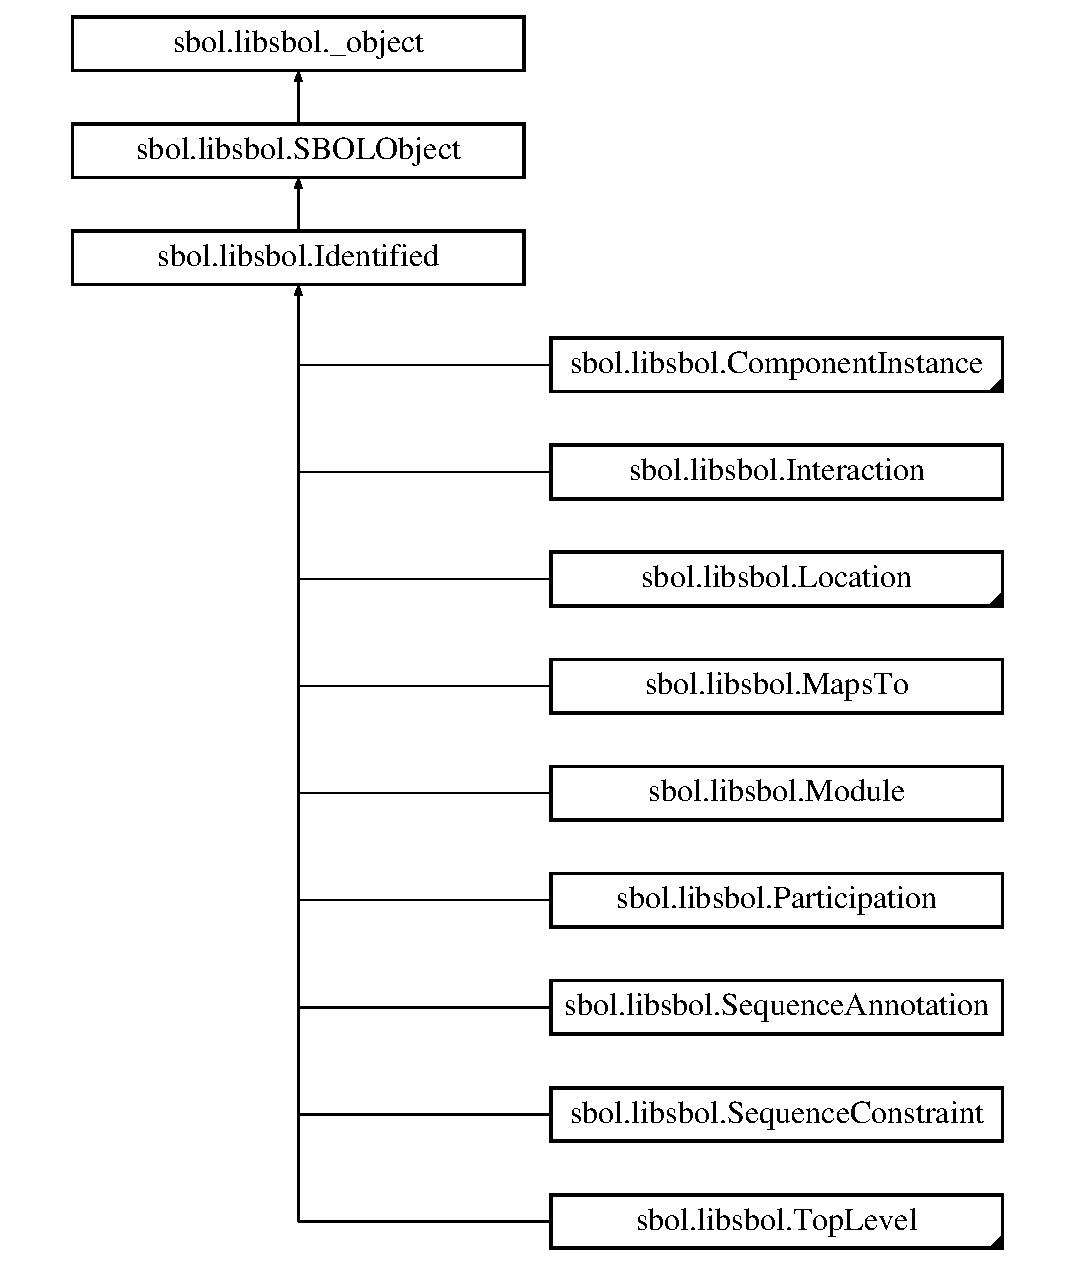
\includegraphics[height=12.000000cm]{classsbol_1_1libsbol_1_1_identified}
\end{center}
\end{figure}
\subsection*{Public Member Functions}
\begin{DoxyCompactItemize}
\item 
def \hyperlink{classsbol_1_1libsbol_1_1_identified_aa88796896d61333684a0991aa1d8734f}{\+\_\+\+\_\+init\+\_\+\+\_\+} (self, args)
\end{DoxyCompactItemize}
\subsection*{Public Attributes}
\begin{DoxyCompactItemize}
\item 
{\bfseries this}\hypertarget{classsbol_1_1libsbol_1_1_identified_aeaddc88dd54cf84e94eb476e2ce1303e}{}\label{classsbol_1_1libsbol_1_1_identified_aeaddc88dd54cf84e94eb476e2ce1303e}

\end{DoxyCompactItemize}
\subsection*{Static Public Attributes}
\begin{DoxyCompactItemize}
\item 
{\bfseries persistent\+Identity} = \+\_\+swig\+\_\+property(\+\_\+libsbol.\+Identified\+\_\+persistent\+Identity\+\_\+get, \+\_\+libsbol.\+Identified\+\_\+persistent\+Identity\+\_\+set)\hypertarget{classsbol_1_1libsbol_1_1_identified_aba54d67c31675ac09eaf1501d8ef4dff}{}\label{classsbol_1_1libsbol_1_1_identified_aba54d67c31675ac09eaf1501d8ef4dff}

\item 
{\bfseries display\+Id} = \+\_\+swig\+\_\+property(\+\_\+libsbol.\+Identified\+\_\+display\+Id\+\_\+get, \+\_\+libsbol.\+Identified\+\_\+display\+Id\+\_\+set)\hypertarget{classsbol_1_1libsbol_1_1_identified_ac71297459486760294dd47f11fa394d3}{}\label{classsbol_1_1libsbol_1_1_identified_ac71297459486760294dd47f11fa394d3}

\item 
{\bfseries version} = \+\_\+swig\+\_\+property(\+\_\+libsbol.\+Identified\+\_\+version\+\_\+get, \+\_\+libsbol.\+Identified\+\_\+version\+\_\+set)\hypertarget{classsbol_1_1libsbol_1_1_identified_a3a2e7d3220478712d087e3000851021f}{}\label{classsbol_1_1libsbol_1_1_identified_a3a2e7d3220478712d087e3000851021f}

\item 
{\bfseries was\+Derived\+From} = \+\_\+swig\+\_\+property(\+\_\+libsbol.\+Identified\+\_\+was\+Derived\+From\+\_\+get, \+\_\+libsbol.\+Identified\+\_\+was\+Derived\+From\+\_\+set)\hypertarget{classsbol_1_1libsbol_1_1_identified_a11aeb7dbdbb811723b72be7a2accf3b4}{}\label{classsbol_1_1libsbol_1_1_identified_a11aeb7dbdbb811723b72be7a2accf3b4}

\item 
{\bfseries name} = \+\_\+swig\+\_\+property(\+\_\+libsbol.\+Identified\+\_\+name\+\_\+get, \+\_\+libsbol.\+Identified\+\_\+name\+\_\+set)\hypertarget{classsbol_1_1libsbol_1_1_identified_a133d7ce431453d6f70ae22676958d9f0}{}\label{classsbol_1_1libsbol_1_1_identified_a133d7ce431453d6f70ae22676958d9f0}

\item 
{\bfseries description} = \+\_\+swig\+\_\+property(\+\_\+libsbol.\+Identified\+\_\+description\+\_\+get, \+\_\+libsbol.\+Identified\+\_\+description\+\_\+set)\hypertarget{classsbol_1_1libsbol_1_1_identified_a8f8ef118afe7f8b1b5c6a567df514368}{}\label{classsbol_1_1libsbol_1_1_identified_a8f8ef118afe7f8b1b5c6a567df514368}

\end{DoxyCompactItemize}


\subsection{Constructor \& Destructor Documentation}
\index{sbol\+::libsbol\+::\+Identified@{sbol\+::libsbol\+::\+Identified}!\+\_\+\+\_\+init\+\_\+\+\_\+@{\+\_\+\+\_\+init\+\_\+\+\_\+}}
\index{\+\_\+\+\_\+init\+\_\+\+\_\+@{\+\_\+\+\_\+init\+\_\+\+\_\+}!sbol\+::libsbol\+::\+Identified@{sbol\+::libsbol\+::\+Identified}}
\subsubsection[{\texorpdfstring{\+\_\+\+\_\+init\+\_\+\+\_\+(self, args)}{__init__(self, args)}}]{\setlength{\rightskip}{0pt plus 5cm}def sbol.\+libsbol.\+Identified.\+\_\+\+\_\+init\+\_\+\+\_\+ (
\begin{DoxyParamCaption}
\item[{}]{self, }
\item[{}]{args}
\end{DoxyParamCaption}
)}\hypertarget{classsbol_1_1libsbol_1_1_identified_aa88796896d61333684a0991aa1d8734f}{}\label{classsbol_1_1libsbol_1_1_identified_aa88796896d61333684a0991aa1d8734f}
\begin{DoxyVerb}sbol::Identified::Identified(std::string prefix, std::string
display_id, std::string version) 
\end{DoxyVerb}
 

The documentation for this class was generated from the following file\+:\begin{DoxyCompactItemize}
\item 
libsbol.\+py\end{DoxyCompactItemize}

\hypertarget{classsbol_1_1libsbol_1_1_interaction}{}\section{sbol.\+libsbol.\+Interaction Class Reference}
\label{classsbol_1_1libsbol_1_1_interaction}\index{sbol.\+libsbol.\+Interaction@{sbol.\+libsbol.\+Interaction}}
Inheritance diagram for sbol.\+libsbol.\+Interaction\+:\begin{figure}[H]
\begin{center}
\leavevmode
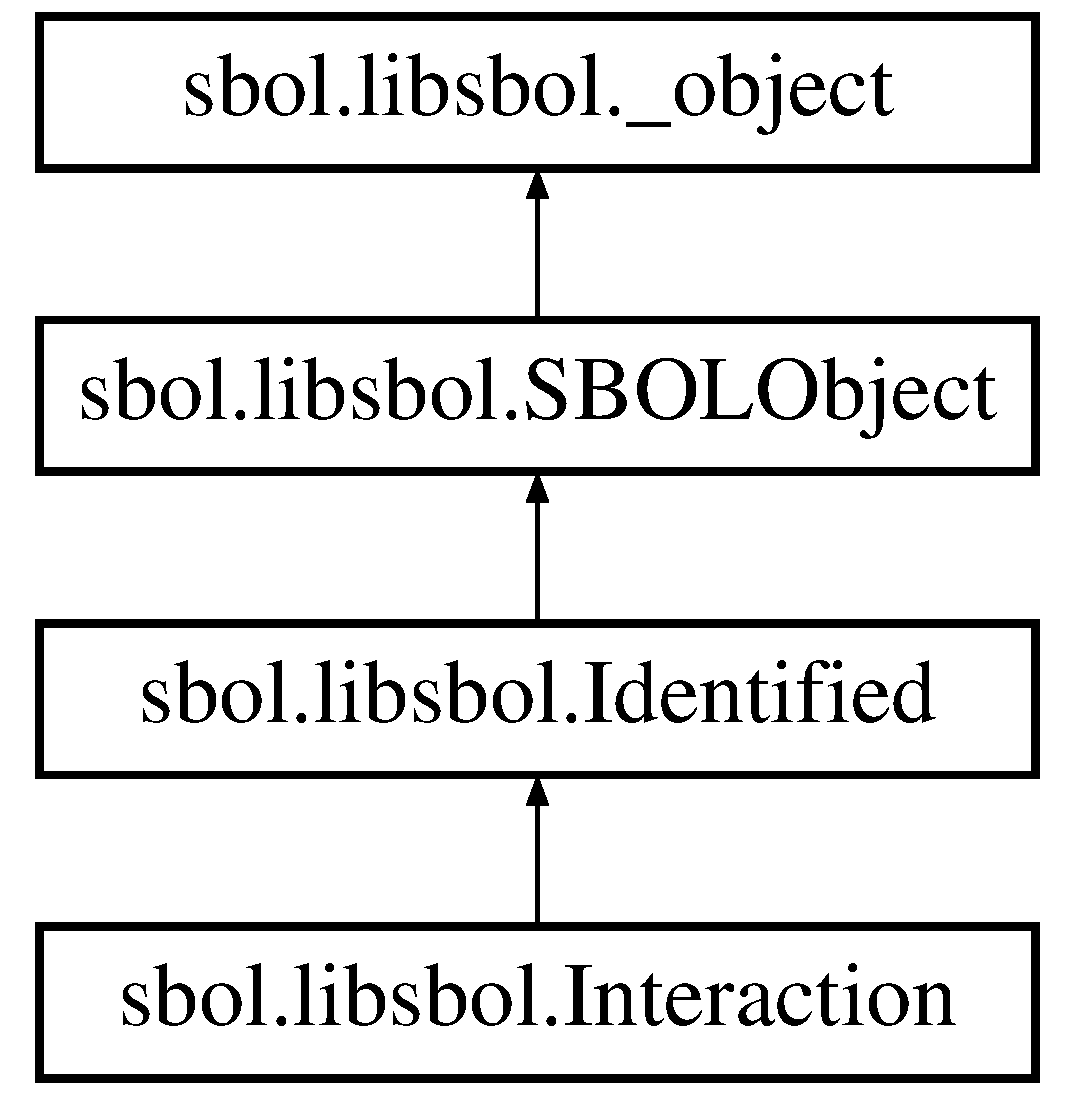
\includegraphics[height=4.000000cm]{classsbol_1_1libsbol_1_1_interaction}
\end{center}
\end{figure}
\subsection*{Public Member Functions}
\begin{DoxyCompactItemize}
\item 
def \hyperlink{classsbol_1_1libsbol_1_1_interaction_a9b81eae3a393df0d5c610f6622408c82}{\+\_\+\+\_\+init\+\_\+\+\_\+} (self, args)
\end{DoxyCompactItemize}
\subsection*{Public Attributes}
\begin{DoxyCompactItemize}
\item 
{\bfseries this}\hypertarget{classsbol_1_1libsbol_1_1_interaction_a29a5965a5a50f41615e780040e39dc02}{}\label{classsbol_1_1libsbol_1_1_interaction_a29a5965a5a50f41615e780040e39dc02}

\end{DoxyCompactItemize}
\subsection*{Static Public Attributes}
\begin{DoxyCompactItemize}
\item 
{\bfseries types} = \+\_\+swig\+\_\+property(\+\_\+libsbol.\+Interaction\+\_\+types\+\_\+get, \+\_\+libsbol.\+Interaction\+\_\+types\+\_\+set)\hypertarget{classsbol_1_1libsbol_1_1_interaction_af2d42822f131c3c838f5044df5668ec4}{}\label{classsbol_1_1libsbol_1_1_interaction_af2d42822f131c3c838f5044df5668ec4}

\item 
{\bfseries participations} = \+\_\+swig\+\_\+property(\+\_\+libsbol.\+Interaction\+\_\+participations\+\_\+get, \+\_\+libsbol.\+Interaction\+\_\+participations\+\_\+set)\hypertarget{classsbol_1_1libsbol_1_1_interaction_a47b065a32a2986546164a16f09c39d57}{}\label{classsbol_1_1libsbol_1_1_interaction_a47b065a32a2986546164a16f09c39d57}

\end{DoxyCompactItemize}


\subsection{Constructor \& Destructor Documentation}
\index{sbol\+::libsbol\+::\+Interaction@{sbol\+::libsbol\+::\+Interaction}!\+\_\+\+\_\+init\+\_\+\+\_\+@{\+\_\+\+\_\+init\+\_\+\+\_\+}}
\index{\+\_\+\+\_\+init\+\_\+\+\_\+@{\+\_\+\+\_\+init\+\_\+\+\_\+}!sbol\+::libsbol\+::\+Interaction@{sbol\+::libsbol\+::\+Interaction}}
\subsubsection[{\texorpdfstring{\+\_\+\+\_\+init\+\_\+\+\_\+(self, args)}{__init__(self, args)}}]{\setlength{\rightskip}{0pt plus 5cm}def sbol.\+libsbol.\+Interaction.\+\_\+\+\_\+init\+\_\+\+\_\+ (
\begin{DoxyParamCaption}
\item[{}]{self, }
\item[{}]{args}
\end{DoxyParamCaption}
)}\hypertarget{classsbol_1_1libsbol_1_1_interaction_a9b81eae3a393df0d5c610f6622408c82}{}\label{classsbol_1_1libsbol_1_1_interaction_a9b81eae3a393df0d5c610f6622408c82}
\begin{DoxyVerb}sbol::Interaction::Interaction(std::string uri_prefix, std::string
display_id, std::string version, std::string interaction_type) 
\end{DoxyVerb}
 

The documentation for this class was generated from the following file\+:\begin{DoxyCompactItemize}
\item 
libsbol.\+py\end{DoxyCompactItemize}

\hypertarget{classsbol_1_1libsbol_1_1interaction_property}{}\section{sbol.\+libsbol.\+interaction\+Property Class Reference}
\label{classsbol_1_1libsbol_1_1interaction_property}\index{sbol.\+libsbol.\+interaction\+Property@{sbol.\+libsbol.\+interaction\+Property}}
Inheritance diagram for sbol.\+libsbol.\+interaction\+Property\+:\begin{figure}[H]
\begin{center}
\leavevmode
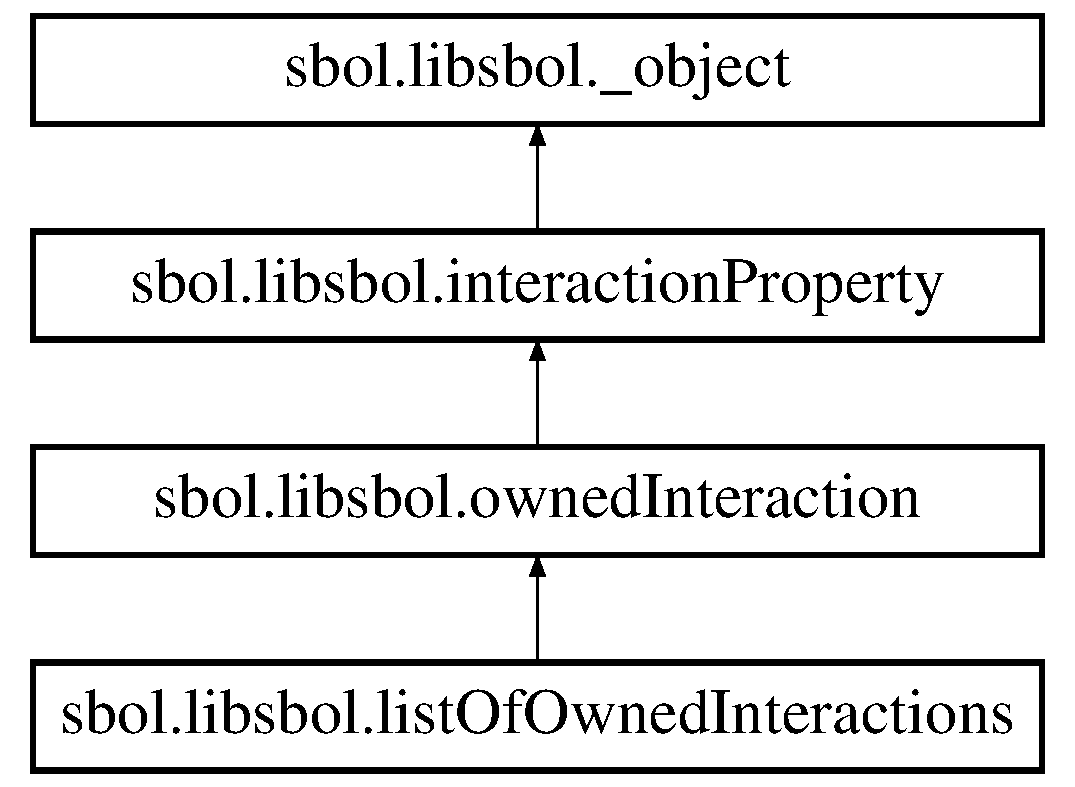
\includegraphics[height=4.000000cm]{classsbol_1_1libsbol_1_1interaction_property}
\end{center}
\end{figure}
\subsection*{Public Member Functions}
\begin{DoxyCompactItemize}
\item 
def \hyperlink{classsbol_1_1libsbol_1_1interaction_property_ad652d4feeb50c02b99b8f50afac5d22f}{\+\_\+\+\_\+init\+\_\+\+\_\+} (self, args)
\item 
def \hyperlink{classsbol_1_1libsbol_1_1interaction_property_a547ad6e60e33b4514cb8a7575fdc12f7}{get\+Type\+U\+RI} (self)
\item 
def \hyperlink{classsbol_1_1libsbol_1_1interaction_property_a5e0cdef68a02528197ad5d8b1390bce9}{get\+Owner} (self)
\item 
def \hyperlink{classsbol_1_1libsbol_1_1interaction_property_aa803bc0b322efe83e2cb5b90a592c530}{get} (self)
\item 
def \hyperlink{classsbol_1_1libsbol_1_1interaction_property_aec96fa010980999b1958b77b9b8b726d}{add} (self, new\+\_\+value)
\item 
def \hyperlink{classsbol_1_1libsbol_1_1interaction_property_ac83de77d39a57272234e72de42931e56}{set} (self, args)
\item 
def \hyperlink{classsbol_1_1libsbol_1_1interaction_property_a215d016ce9a285e831f9acef4c88c90b}{write} (self)
\item 
def \hyperlink{classsbol_1_1libsbol_1_1interaction_property_a0e22ee1d58678c7ecddad76106e05b19}{validate} (self, arg=None)
\item 
def {\bfseries \+\_\+\+\_\+getitem\+\_\+\+\_\+} (self, n\+Index)\hypertarget{classsbol_1_1libsbol_1_1interaction_property_a63c7d05f9302cad2518ff05c4e75508a}{}\label{classsbol_1_1libsbol_1_1interaction_property_a63c7d05f9302cad2518ff05c4e75508a}

\item 
def {\bfseries \+\_\+\+\_\+iter\+\_\+\+\_\+} (self)\hypertarget{classsbol_1_1libsbol_1_1interaction_property_a69f2f01b3b857e2c098290f2fd7ce767}{}\label{classsbol_1_1libsbol_1_1interaction_property_a69f2f01b3b857e2c098290f2fd7ce767}

\item 
def {\bfseries next} (self)\hypertarget{classsbol_1_1libsbol_1_1interaction_property_add20b9e20d66e4575c37ad49868b428c}{}\label{classsbol_1_1libsbol_1_1interaction_property_add20b9e20d66e4575c37ad49868b428c}

\item 
def {\bfseries \+\_\+\+\_\+len\+\_\+\+\_\+} (self)\hypertarget{classsbol_1_1libsbol_1_1interaction_property_abad413414264a45465140f43d5c3a6a7}{}\label{classsbol_1_1libsbol_1_1interaction_property_abad413414264a45465140f43d5c3a6a7}

\end{DoxyCompactItemize}
\subsection*{Public Attributes}
\begin{DoxyCompactItemize}
\item 
{\bfseries this}\hypertarget{classsbol_1_1libsbol_1_1interaction_property_a7e69b529aba385073380a10585e801b7}{}\label{classsbol_1_1libsbol_1_1interaction_property_a7e69b529aba385073380a10585e801b7}

\end{DoxyCompactItemize}


\subsection{Detailed Description}
\begin{DoxyVerb}metafunction for generation of a map of message types to their
associated callbacks.

Usage: Use generate_callback_map<Type>::type to ...

Parameters:
-----------

LiteralType:  The library currently supports Property<string> and
Property<int> specification currently supports integer, string, and
URI literals

C++ includes: property.h 
\end{DoxyVerb}
 

\subsection{Constructor \& Destructor Documentation}
\index{sbol\+::libsbol\+::interaction\+Property@{sbol\+::libsbol\+::interaction\+Property}!\+\_\+\+\_\+init\+\_\+\+\_\+@{\+\_\+\+\_\+init\+\_\+\+\_\+}}
\index{\+\_\+\+\_\+init\+\_\+\+\_\+@{\+\_\+\+\_\+init\+\_\+\+\_\+}!sbol\+::libsbol\+::interaction\+Property@{sbol\+::libsbol\+::interaction\+Property}}
\subsubsection[{\texorpdfstring{\+\_\+\+\_\+init\+\_\+\+\_\+(self, args)}{__init__(self, args)}}]{\setlength{\rightskip}{0pt plus 5cm}def sbol.\+libsbol.\+interaction\+Property.\+\_\+\+\_\+init\+\_\+\+\_\+ (
\begin{DoxyParamCaption}
\item[{}]{self, }
\item[{}]{args}
\end{DoxyParamCaption}
)}\hypertarget{classsbol_1_1libsbol_1_1interaction_property_ad652d4feeb50c02b99b8f50afac5d22f}{}\label{classsbol_1_1libsbol_1_1interaction_property_ad652d4feeb50c02b99b8f50afac5d22f}
\begin{DoxyVerb}sbol::Property<
LiteralType >::Property(sbol_type type_uri=UNDEFINED, void
*property_owner=NULL, ValidationRules validation_rules={}) 
\end{DoxyVerb}
 

\subsection{Member Function Documentation}
\index{sbol\+::libsbol\+::interaction\+Property@{sbol\+::libsbol\+::interaction\+Property}!add@{add}}
\index{add@{add}!sbol\+::libsbol\+::interaction\+Property@{sbol\+::libsbol\+::interaction\+Property}}
\subsubsection[{\texorpdfstring{add(self, new\+\_\+value)}{add(self, new_value)}}]{\setlength{\rightskip}{0pt plus 5cm}def sbol.\+libsbol.\+interaction\+Property.\+add (
\begin{DoxyParamCaption}
\item[{}]{self, }
\item[{}]{new\+\_\+value}
\end{DoxyParamCaption}
)}\hypertarget{classsbol_1_1libsbol_1_1interaction_property_aec96fa010980999b1958b77b9b8b726d}{}\label{classsbol_1_1libsbol_1_1interaction_property_aec96fa010980999b1958b77b9b8b726d}
\begin{DoxyVerb}void sbol::Property<
LiteralType >::add(std::string new_value) 
\end{DoxyVerb}
 \index{sbol\+::libsbol\+::interaction\+Property@{sbol\+::libsbol\+::interaction\+Property}!get@{get}}
\index{get@{get}!sbol\+::libsbol\+::interaction\+Property@{sbol\+::libsbol\+::interaction\+Property}}
\subsubsection[{\texorpdfstring{get(self)}{get(self)}}]{\setlength{\rightskip}{0pt plus 5cm}def sbol.\+libsbol.\+interaction\+Property.\+get (
\begin{DoxyParamCaption}
\item[{}]{self}
\end{DoxyParamCaption}
)}\hypertarget{classsbol_1_1libsbol_1_1interaction_property_aa803bc0b322efe83e2cb5b90a592c530}{}\label{classsbol_1_1libsbol_1_1interaction_property_aa803bc0b322efe83e2cb5b90a592c530}
\begin{DoxyVerb}std::string
sbol::Property< LiteralType >::get() 
\end{DoxyVerb}
 \index{sbol\+::libsbol\+::interaction\+Property@{sbol\+::libsbol\+::interaction\+Property}!get\+Owner@{get\+Owner}}
\index{get\+Owner@{get\+Owner}!sbol\+::libsbol\+::interaction\+Property@{sbol\+::libsbol\+::interaction\+Property}}
\subsubsection[{\texorpdfstring{get\+Owner(self)}{getOwner(self)}}]{\setlength{\rightskip}{0pt plus 5cm}def sbol.\+libsbol.\+interaction\+Property.\+get\+Owner (
\begin{DoxyParamCaption}
\item[{}]{self}
\end{DoxyParamCaption}
)}\hypertarget{classsbol_1_1libsbol_1_1interaction_property_a5e0cdef68a02528197ad5d8b1390bce9}{}\label{classsbol_1_1libsbol_1_1interaction_property_a5e0cdef68a02528197ad5d8b1390bce9}
\begin{DoxyVerb}SBOLObject &
sbol::Property< LiteralType >::getOwner() 
\end{DoxyVerb}
 \index{sbol\+::libsbol\+::interaction\+Property@{sbol\+::libsbol\+::interaction\+Property}!get\+Type\+U\+RI@{get\+Type\+U\+RI}}
\index{get\+Type\+U\+RI@{get\+Type\+U\+RI}!sbol\+::libsbol\+::interaction\+Property@{sbol\+::libsbol\+::interaction\+Property}}
\subsubsection[{\texorpdfstring{get\+Type\+U\+R\+I(self)}{getTypeURI(self)}}]{\setlength{\rightskip}{0pt plus 5cm}def sbol.\+libsbol.\+interaction\+Property.\+get\+Type\+U\+RI (
\begin{DoxyParamCaption}
\item[{}]{self}
\end{DoxyParamCaption}
)}\hypertarget{classsbol_1_1libsbol_1_1interaction_property_a547ad6e60e33b4514cb8a7575fdc12f7}{}\label{classsbol_1_1libsbol_1_1interaction_property_a547ad6e60e33b4514cb8a7575fdc12f7}
\begin{DoxyVerb}sbol_type
sbol::Property< LiteralType >::getTypeURI() 
\end{DoxyVerb}
 \index{sbol\+::libsbol\+::interaction\+Property@{sbol\+::libsbol\+::interaction\+Property}!set@{set}}
\index{set@{set}!sbol\+::libsbol\+::interaction\+Property@{sbol\+::libsbol\+::interaction\+Property}}
\subsubsection[{\texorpdfstring{set(self, args)}{set(self, args)}}]{\setlength{\rightskip}{0pt plus 5cm}def sbol.\+libsbol.\+interaction\+Property.\+set (
\begin{DoxyParamCaption}
\item[{}]{self, }
\item[{}]{args}
\end{DoxyParamCaption}
)}\hypertarget{classsbol_1_1libsbol_1_1interaction_property_ac83de77d39a57272234e72de42931e56}{}\label{classsbol_1_1libsbol_1_1interaction_property_ac83de77d39a57272234e72de42931e56}
\begin{DoxyVerb}void sbol::Property<
LiteralType >::set(int new_value) 
\end{DoxyVerb}
 \index{sbol\+::libsbol\+::interaction\+Property@{sbol\+::libsbol\+::interaction\+Property}!validate@{validate}}
\index{validate@{validate}!sbol\+::libsbol\+::interaction\+Property@{sbol\+::libsbol\+::interaction\+Property}}
\subsubsection[{\texorpdfstring{validate(self, arg=\+None)}{validate(self, arg=None)}}]{\setlength{\rightskip}{0pt plus 5cm}def sbol.\+libsbol.\+interaction\+Property.\+validate (
\begin{DoxyParamCaption}
\item[{}]{self, }
\item[{}]{arg = {\ttfamily None}}
\end{DoxyParamCaption}
)}\hypertarget{classsbol_1_1libsbol_1_1interaction_property_a0e22ee1d58678c7ecddad76106e05b19}{}\label{classsbol_1_1libsbol_1_1interaction_property_a0e22ee1d58678c7ecddad76106e05b19}
\begin{DoxyVerb}void sbol::Property<
LiteralType >::validate(void *arg=NULL) 
\end{DoxyVerb}
 \index{sbol\+::libsbol\+::interaction\+Property@{sbol\+::libsbol\+::interaction\+Property}!write@{write}}
\index{write@{write}!sbol\+::libsbol\+::interaction\+Property@{sbol\+::libsbol\+::interaction\+Property}}
\subsubsection[{\texorpdfstring{write(self)}{write(self)}}]{\setlength{\rightskip}{0pt plus 5cm}def sbol.\+libsbol.\+interaction\+Property.\+write (
\begin{DoxyParamCaption}
\item[{}]{self}
\end{DoxyParamCaption}
)}\hypertarget{classsbol_1_1libsbol_1_1interaction_property_a215d016ce9a285e831f9acef4c88c90b}{}\label{classsbol_1_1libsbol_1_1interaction_property_a215d016ce9a285e831f9acef4c88c90b}
\begin{DoxyVerb}void sbol::Property<
LiteralType >::write() 
\end{DoxyVerb}
 

The documentation for this class was generated from the following file\+:\begin{DoxyCompactItemize}
\item 
libsbol.\+py\end{DoxyCompactItemize}

\hypertarget{classsbol_1_1libsbol_1_1_int_property}{}\section{sbol.\+libsbol.\+Int\+Property Class Reference}
\label{classsbol_1_1libsbol_1_1_int_property}\index{sbol.\+libsbol.\+Int\+Property@{sbol.\+libsbol.\+Int\+Property}}
Inheritance diagram for sbol.\+libsbol.\+Int\+Property\+:\begin{figure}[H]
\begin{center}
\leavevmode
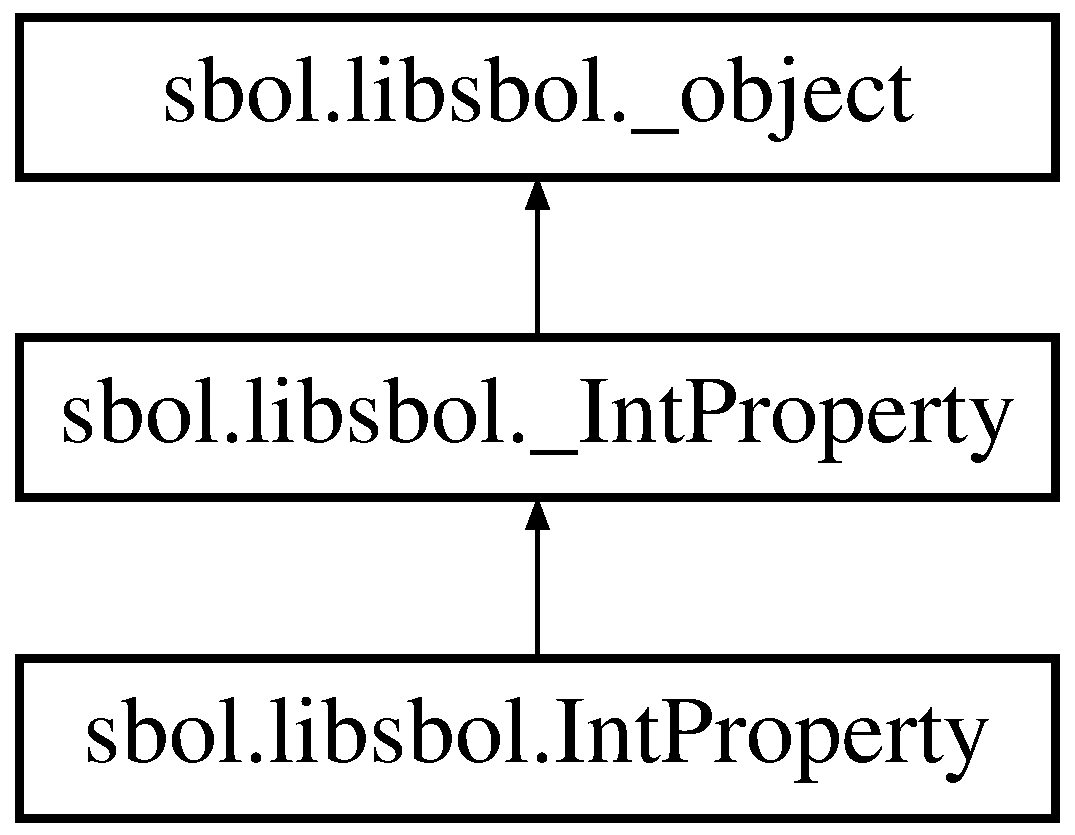
\includegraphics[height=3.000000cm]{classsbol_1_1libsbol_1_1_int_property}
\end{center}
\end{figure}
\subsection*{Public Member Functions}
\begin{DoxyCompactItemize}
\item 
def \hyperlink{classsbol_1_1libsbol_1_1_int_property_ac7205486fd84370791340cbef97adfc4}{\+\_\+\+\_\+init\+\_\+\+\_\+} (self, type\+\_\+uri, property\+\_\+owner, initial\+\_\+value=0)
\end{DoxyCompactItemize}
\subsection*{Public Attributes}
\begin{DoxyCompactItemize}
\item 
{\bfseries this}\hypertarget{classsbol_1_1libsbol_1_1_int_property_a2476b79229067f72732b3279f66bef96}{}\label{classsbol_1_1libsbol_1_1_int_property_a2476b79229067f72732b3279f66bef96}

\end{DoxyCompactItemize}


\subsection{Constructor \& Destructor Documentation}
\index{sbol\+::libsbol\+::\+Int\+Property@{sbol\+::libsbol\+::\+Int\+Property}!\+\_\+\+\_\+init\+\_\+\+\_\+@{\+\_\+\+\_\+init\+\_\+\+\_\+}}
\index{\+\_\+\+\_\+init\+\_\+\+\_\+@{\+\_\+\+\_\+init\+\_\+\+\_\+}!sbol\+::libsbol\+::\+Int\+Property@{sbol\+::libsbol\+::\+Int\+Property}}
\subsubsection[{\texorpdfstring{\+\_\+\+\_\+init\+\_\+\+\_\+(self, type\+\_\+uri, property\+\_\+owner, initial\+\_\+value=0)}{__init__(self, type_uri, property_owner, initial_value=0)}}]{\setlength{\rightskip}{0pt plus 5cm}def sbol.\+libsbol.\+Int\+Property.\+\_\+\+\_\+init\+\_\+\+\_\+ (
\begin{DoxyParamCaption}
\item[{}]{self, }
\item[{}]{type\+\_\+uri, }
\item[{}]{property\+\_\+owner, }
\item[{}]{initial\+\_\+value = {\ttfamily 0}}
\end{DoxyParamCaption}
)}\hypertarget{classsbol_1_1libsbol_1_1_int_property_ac7205486fd84370791340cbef97adfc4}{}\label{classsbol_1_1libsbol_1_1_int_property_ac7205486fd84370791340cbef97adfc4}
\begin{DoxyVerb}sbol::IntProperty::IntProperty(sbol_type type_uri, void
*property_owner, int initial_value=0) 
\end{DoxyVerb}
 

The documentation for this class was generated from the following file\+:\begin{DoxyCompactItemize}
\item 
libsbol.\+py\end{DoxyCompactItemize}

\hypertarget{classsbol_1_1libsbol_1_1list_of_owned_functional_components}{}\section{sbol.\+libsbol.\+list\+Of\+Owned\+Functional\+Components Class Reference}
\label{classsbol_1_1libsbol_1_1list_of_owned_functional_components}\index{sbol.\+libsbol.\+list\+Of\+Owned\+Functional\+Components@{sbol.\+libsbol.\+list\+Of\+Owned\+Functional\+Components}}
Inheritance diagram for sbol.\+libsbol.\+list\+Of\+Owned\+Functional\+Components\+:\begin{figure}[H]
\begin{center}
\leavevmode
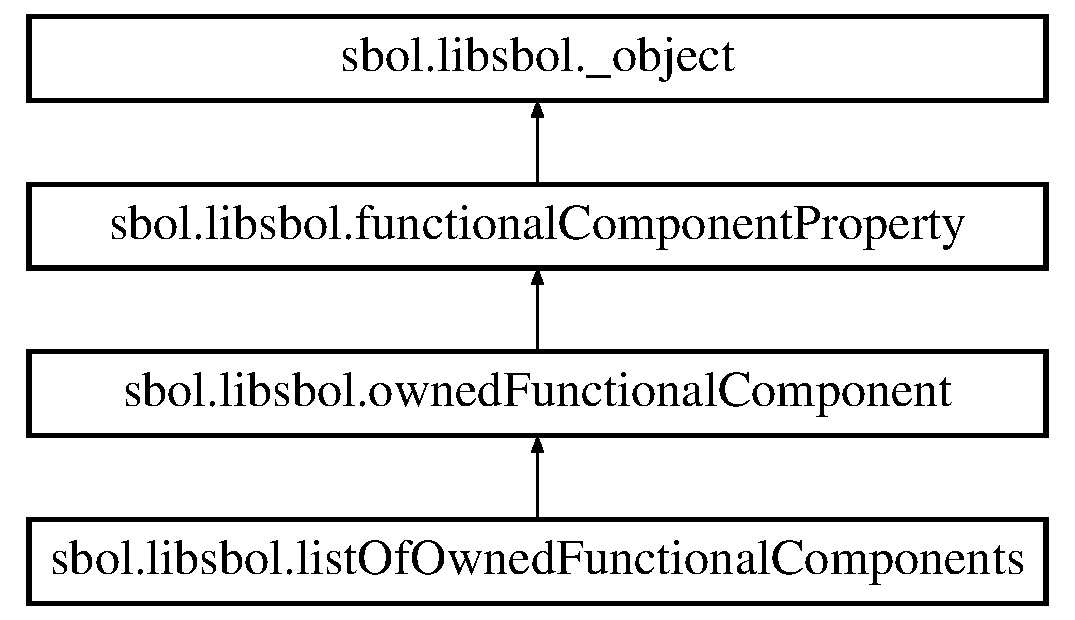
\includegraphics[height=4.000000cm]{classsbol_1_1libsbol_1_1list_of_owned_functional_components}
\end{center}
\end{figure}
\subsection*{Public Member Functions}
\begin{DoxyCompactItemize}
\item 
def \hyperlink{classsbol_1_1libsbol_1_1list_of_owned_functional_components_af0b2a415e4bf2e45c34c522c71a2bce7}{\+\_\+\+\_\+init\+\_\+\+\_\+} (self, args)
\item 
def \hyperlink{classsbol_1_1libsbol_1_1list_of_owned_functional_components_adc82fb9d19fa1c4d4e88d0080b9c11dc}{remove} (self, index)
\end{DoxyCompactItemize}
\subsection*{Public Attributes}
\begin{DoxyCompactItemize}
\item 
{\bfseries this}\hypertarget{classsbol_1_1libsbol_1_1list_of_owned_functional_components_a0eb7dcb9005fa180fcb396b1937d5464}{}\label{classsbol_1_1libsbol_1_1list_of_owned_functional_components_a0eb7dcb9005fa180fcb396b1937d5464}

\end{DoxyCompactItemize}
\subsection*{Additional Inherited Members}


\subsection{Constructor \& Destructor Documentation}
\index{sbol\+::libsbol\+::list\+Of\+Owned\+Functional\+Components@{sbol\+::libsbol\+::list\+Of\+Owned\+Functional\+Components}!\+\_\+\+\_\+init\+\_\+\+\_\+@{\+\_\+\+\_\+init\+\_\+\+\_\+}}
\index{\+\_\+\+\_\+init\+\_\+\+\_\+@{\+\_\+\+\_\+init\+\_\+\+\_\+}!sbol\+::libsbol\+::list\+Of\+Owned\+Functional\+Components@{sbol\+::libsbol\+::list\+Of\+Owned\+Functional\+Components}}
\subsubsection[{\texorpdfstring{\+\_\+\+\_\+init\+\_\+\+\_\+(self, args)}{__init__(self, args)}}]{\setlength{\rightskip}{0pt plus 5cm}def sbol.\+libsbol.\+list\+Of\+Owned\+Functional\+Components.\+\_\+\+\_\+init\+\_\+\+\_\+ (
\begin{DoxyParamCaption}
\item[{}]{self, }
\item[{}]{args}
\end{DoxyParamCaption}
)}\hypertarget{classsbol_1_1libsbol_1_1list_of_owned_functional_components_af0b2a415e4bf2e45c34c522c71a2bce7}{}\label{classsbol_1_1libsbol_1_1list_of_owned_functional_components_af0b2a415e4bf2e45c34c522c71a2bce7}
\begin{DoxyVerb}sbol::List< PropertyType
>::List(sbol_type type_uri, SBOLObject *property_owner, std::string
initial_value="") 
\end{DoxyVerb}
 

\subsection{Member Function Documentation}
\index{sbol\+::libsbol\+::list\+Of\+Owned\+Functional\+Components@{sbol\+::libsbol\+::list\+Of\+Owned\+Functional\+Components}!remove@{remove}}
\index{remove@{remove}!sbol\+::libsbol\+::list\+Of\+Owned\+Functional\+Components@{sbol\+::libsbol\+::list\+Of\+Owned\+Functional\+Components}}
\subsubsection[{\texorpdfstring{remove(self, index)}{remove(self, index)}}]{\setlength{\rightskip}{0pt plus 5cm}def sbol.\+libsbol.\+list\+Of\+Owned\+Functional\+Components.\+remove (
\begin{DoxyParamCaption}
\item[{}]{self, }
\item[{}]{index}
\end{DoxyParamCaption}
)}\hypertarget{classsbol_1_1libsbol_1_1list_of_owned_functional_components_adc82fb9d19fa1c4d4e88d0080b9c11dc}{}\label{classsbol_1_1libsbol_1_1list_of_owned_functional_components_adc82fb9d19fa1c4d4e88d0080b9c11dc}
\begin{DoxyVerb}void sbol::List<
PropertyType >::remove(int index) 
\end{DoxyVerb}
 

The documentation for this class was generated from the following file\+:\begin{DoxyCompactItemize}
\item 
libsbol.\+py\end{DoxyCompactItemize}

\hypertarget{classsbol_1_1libsbol_1_1list_of_owned_interactions}{}\section{sbol.\+libsbol.\+list\+Of\+Owned\+Interactions Class Reference}
\label{classsbol_1_1libsbol_1_1list_of_owned_interactions}\index{sbol.\+libsbol.\+list\+Of\+Owned\+Interactions@{sbol.\+libsbol.\+list\+Of\+Owned\+Interactions}}
Inheritance diagram for sbol.\+libsbol.\+list\+Of\+Owned\+Interactions\+:\begin{figure}[H]
\begin{center}
\leavevmode
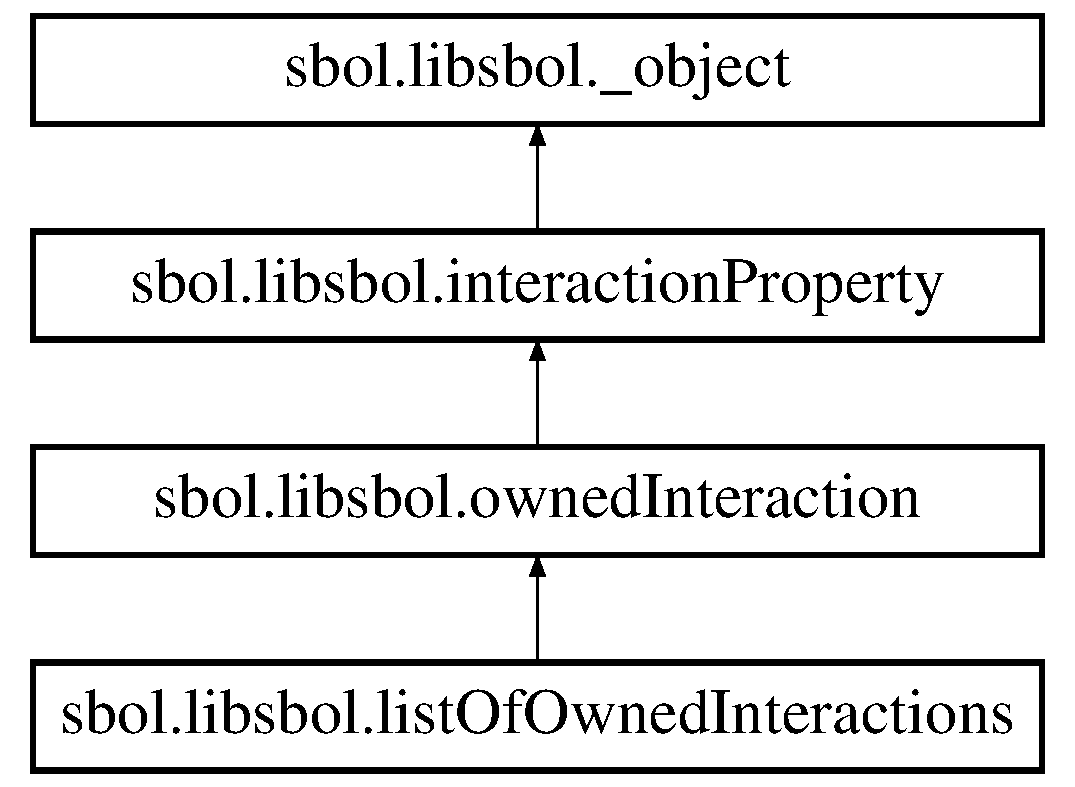
\includegraphics[height=4.000000cm]{classsbol_1_1libsbol_1_1list_of_owned_interactions}
\end{center}
\end{figure}
\subsection*{Public Member Functions}
\begin{DoxyCompactItemize}
\item 
def \hyperlink{classsbol_1_1libsbol_1_1list_of_owned_interactions_a81b00321a0ec3ee210a57a41ddbac656}{\+\_\+\+\_\+init\+\_\+\+\_\+} (self, args)
\item 
def \hyperlink{classsbol_1_1libsbol_1_1list_of_owned_interactions_ac57156b5a021974626617e4e5775f6aa}{remove} (self, index)
\end{DoxyCompactItemize}
\subsection*{Public Attributes}
\begin{DoxyCompactItemize}
\item 
{\bfseries this}\hypertarget{classsbol_1_1libsbol_1_1list_of_owned_interactions_aed8ac6dcc8c52f7901b8eda1b0358f03}{}\label{classsbol_1_1libsbol_1_1list_of_owned_interactions_aed8ac6dcc8c52f7901b8eda1b0358f03}

\end{DoxyCompactItemize}
\subsection*{Additional Inherited Members}


\subsection{Constructor \& Destructor Documentation}
\index{sbol\+::libsbol\+::list\+Of\+Owned\+Interactions@{sbol\+::libsbol\+::list\+Of\+Owned\+Interactions}!\+\_\+\+\_\+init\+\_\+\+\_\+@{\+\_\+\+\_\+init\+\_\+\+\_\+}}
\index{\+\_\+\+\_\+init\+\_\+\+\_\+@{\+\_\+\+\_\+init\+\_\+\+\_\+}!sbol\+::libsbol\+::list\+Of\+Owned\+Interactions@{sbol\+::libsbol\+::list\+Of\+Owned\+Interactions}}
\subsubsection[{\texorpdfstring{\+\_\+\+\_\+init\+\_\+\+\_\+(self, args)}{__init__(self, args)}}]{\setlength{\rightskip}{0pt plus 5cm}def sbol.\+libsbol.\+list\+Of\+Owned\+Interactions.\+\_\+\+\_\+init\+\_\+\+\_\+ (
\begin{DoxyParamCaption}
\item[{}]{self, }
\item[{}]{args}
\end{DoxyParamCaption}
)}\hypertarget{classsbol_1_1libsbol_1_1list_of_owned_interactions_a81b00321a0ec3ee210a57a41ddbac656}{}\label{classsbol_1_1libsbol_1_1list_of_owned_interactions_a81b00321a0ec3ee210a57a41ddbac656}
\begin{DoxyVerb}sbol::List< PropertyType
>::List(sbol_type type_uri, SBOLObject *property_owner, std::string
initial_value="") 
\end{DoxyVerb}
 

\subsection{Member Function Documentation}
\index{sbol\+::libsbol\+::list\+Of\+Owned\+Interactions@{sbol\+::libsbol\+::list\+Of\+Owned\+Interactions}!remove@{remove}}
\index{remove@{remove}!sbol\+::libsbol\+::list\+Of\+Owned\+Interactions@{sbol\+::libsbol\+::list\+Of\+Owned\+Interactions}}
\subsubsection[{\texorpdfstring{remove(self, index)}{remove(self, index)}}]{\setlength{\rightskip}{0pt plus 5cm}def sbol.\+libsbol.\+list\+Of\+Owned\+Interactions.\+remove (
\begin{DoxyParamCaption}
\item[{}]{self, }
\item[{}]{index}
\end{DoxyParamCaption}
)}\hypertarget{classsbol_1_1libsbol_1_1list_of_owned_interactions_ac57156b5a021974626617e4e5775f6aa}{}\label{classsbol_1_1libsbol_1_1list_of_owned_interactions_ac57156b5a021974626617e4e5775f6aa}
\begin{DoxyVerb}void sbol::List<
PropertyType >::remove(int index) 
\end{DoxyVerb}
 

The documentation for this class was generated from the following file\+:\begin{DoxyCompactItemize}
\item 
libsbol.\+py\end{DoxyCompactItemize}

\hypertarget{classsbol_1_1libsbol_1_1list_of_owned_locations}{}\section{sbol.\+libsbol.\+list\+Of\+Owned\+Locations Class Reference}
\label{classsbol_1_1libsbol_1_1list_of_owned_locations}\index{sbol.\+libsbol.\+list\+Of\+Owned\+Locations@{sbol.\+libsbol.\+list\+Of\+Owned\+Locations}}
Inheritance diagram for sbol.\+libsbol.\+list\+Of\+Owned\+Locations\+:\begin{figure}[H]
\begin{center}
\leavevmode
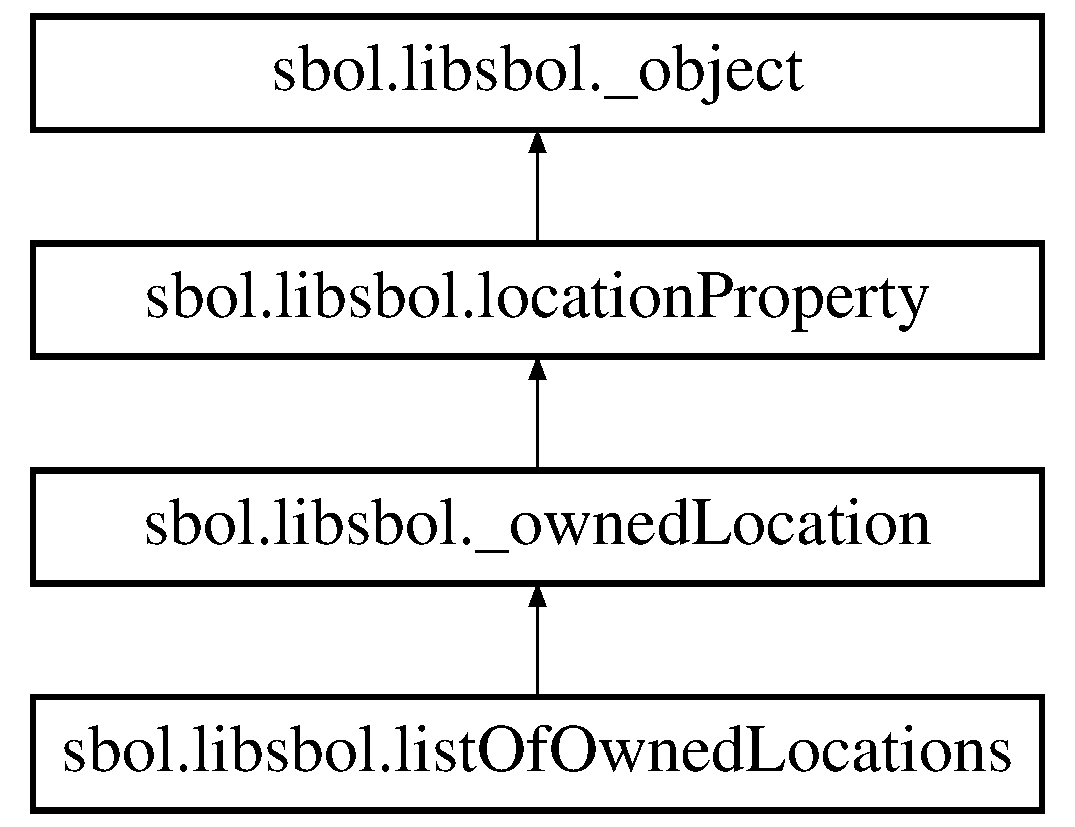
\includegraphics[height=4.000000cm]{classsbol_1_1libsbol_1_1list_of_owned_locations}
\end{center}
\end{figure}
\subsection*{Public Member Functions}
\begin{DoxyCompactItemize}
\item 
def \hyperlink{classsbol_1_1libsbol_1_1list_of_owned_locations_a7991669445a8ce973bf3716407f21499}{\+\_\+\+\_\+init\+\_\+\+\_\+} (self, args)
\item 
def \hyperlink{classsbol_1_1libsbol_1_1list_of_owned_locations_a8785265da5a3d3f5cdfaeddd6e9ddd92}{remove} (self, index)
\end{DoxyCompactItemize}
\subsection*{Public Attributes}
\begin{DoxyCompactItemize}
\item 
{\bfseries this}\hypertarget{classsbol_1_1libsbol_1_1list_of_owned_locations_a68d26a4fbafaea330d41e9d3a0f9ba1b}{}\label{classsbol_1_1libsbol_1_1list_of_owned_locations_a68d26a4fbafaea330d41e9d3a0f9ba1b}

\end{DoxyCompactItemize}
\subsection*{Additional Inherited Members}


\subsection{Constructor \& Destructor Documentation}
\index{sbol\+::libsbol\+::list\+Of\+Owned\+Locations@{sbol\+::libsbol\+::list\+Of\+Owned\+Locations}!\+\_\+\+\_\+init\+\_\+\+\_\+@{\+\_\+\+\_\+init\+\_\+\+\_\+}}
\index{\+\_\+\+\_\+init\+\_\+\+\_\+@{\+\_\+\+\_\+init\+\_\+\+\_\+}!sbol\+::libsbol\+::list\+Of\+Owned\+Locations@{sbol\+::libsbol\+::list\+Of\+Owned\+Locations}}
\subsubsection[{\texorpdfstring{\+\_\+\+\_\+init\+\_\+\+\_\+(self, args)}{__init__(self, args)}}]{\setlength{\rightskip}{0pt plus 5cm}def sbol.\+libsbol.\+list\+Of\+Owned\+Locations.\+\_\+\+\_\+init\+\_\+\+\_\+ (
\begin{DoxyParamCaption}
\item[{}]{self, }
\item[{}]{args}
\end{DoxyParamCaption}
)}\hypertarget{classsbol_1_1libsbol_1_1list_of_owned_locations_a7991669445a8ce973bf3716407f21499}{}\label{classsbol_1_1libsbol_1_1list_of_owned_locations_a7991669445a8ce973bf3716407f21499}
\begin{DoxyVerb}sbol::List< PropertyType
>::List(sbol_type type_uri, SBOLObject *property_owner, std::string
initial_value="") 
\end{DoxyVerb}
 

\subsection{Member Function Documentation}
\index{sbol\+::libsbol\+::list\+Of\+Owned\+Locations@{sbol\+::libsbol\+::list\+Of\+Owned\+Locations}!remove@{remove}}
\index{remove@{remove}!sbol\+::libsbol\+::list\+Of\+Owned\+Locations@{sbol\+::libsbol\+::list\+Of\+Owned\+Locations}}
\subsubsection[{\texorpdfstring{remove(self, index)}{remove(self, index)}}]{\setlength{\rightskip}{0pt plus 5cm}def sbol.\+libsbol.\+list\+Of\+Owned\+Locations.\+remove (
\begin{DoxyParamCaption}
\item[{}]{self, }
\item[{}]{index}
\end{DoxyParamCaption}
)}\hypertarget{classsbol_1_1libsbol_1_1list_of_owned_locations_a8785265da5a3d3f5cdfaeddd6e9ddd92}{}\label{classsbol_1_1libsbol_1_1list_of_owned_locations_a8785265da5a3d3f5cdfaeddd6e9ddd92}
\begin{DoxyVerb}void sbol::List<
PropertyType >::remove(int index) 
\end{DoxyVerb}
 

The documentation for this class was generated from the following file\+:\begin{DoxyCompactItemize}
\item 
libsbol.\+py\end{DoxyCompactItemize}

\hypertarget{classsbol_1_1libsbol_1_1list_of_owned_maps_tos}{}\section{sbol.\+libsbol.\+list\+Of\+Owned\+Maps\+Tos Class Reference}
\label{classsbol_1_1libsbol_1_1list_of_owned_maps_tos}\index{sbol.\+libsbol.\+list\+Of\+Owned\+Maps\+Tos@{sbol.\+libsbol.\+list\+Of\+Owned\+Maps\+Tos}}
Inheritance diagram for sbol.\+libsbol.\+list\+Of\+Owned\+Maps\+Tos\+:\begin{figure}[H]
\begin{center}
\leavevmode
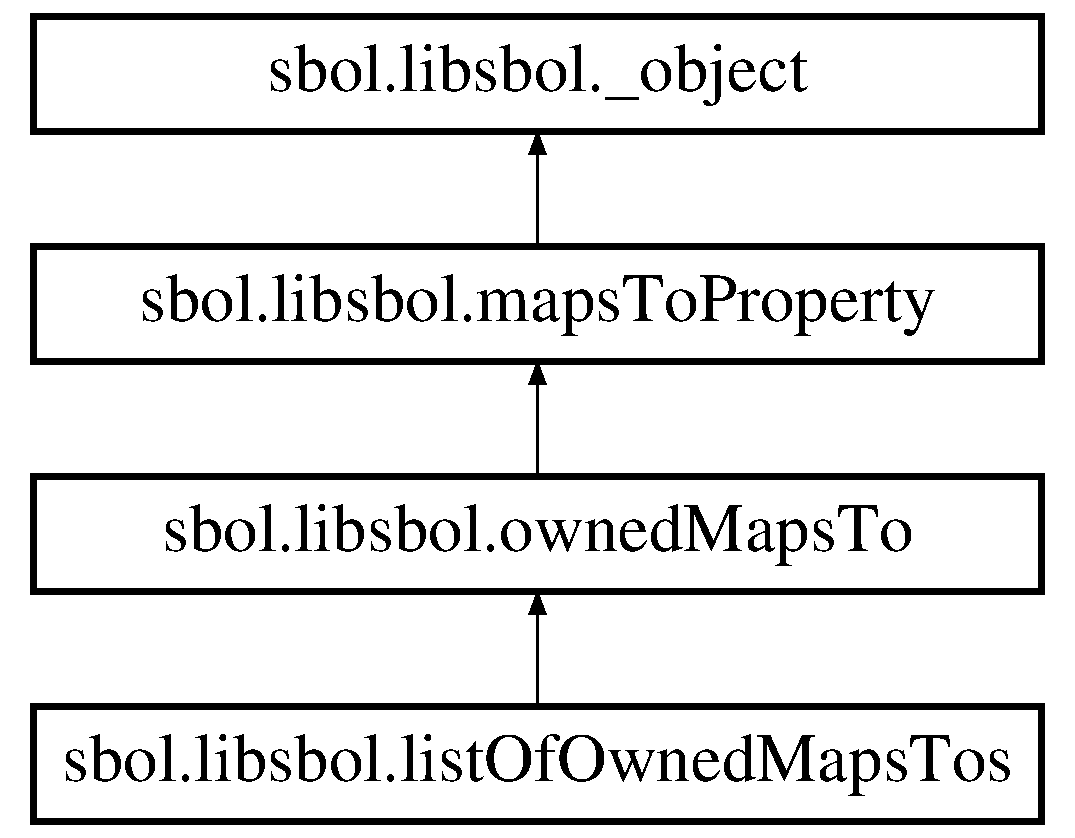
\includegraphics[height=4.000000cm]{classsbol_1_1libsbol_1_1list_of_owned_maps_tos}
\end{center}
\end{figure}
\subsection*{Public Member Functions}
\begin{DoxyCompactItemize}
\item 
def \hyperlink{classsbol_1_1libsbol_1_1list_of_owned_maps_tos_a50b6e2a8b7b51f1189e03cea6b4b94ff}{\+\_\+\+\_\+init\+\_\+\+\_\+} (self, args)
\item 
def \hyperlink{classsbol_1_1libsbol_1_1list_of_owned_maps_tos_a02b1f23496c8b32dbd70cd156b0f23e1}{remove} (self, index)
\end{DoxyCompactItemize}
\subsection*{Public Attributes}
\begin{DoxyCompactItemize}
\item 
{\bfseries this}\hypertarget{classsbol_1_1libsbol_1_1list_of_owned_maps_tos_a90d0c2fc442abb23a8094d14cd6c6ee9}{}\label{classsbol_1_1libsbol_1_1list_of_owned_maps_tos_a90d0c2fc442abb23a8094d14cd6c6ee9}

\end{DoxyCompactItemize}
\subsection*{Additional Inherited Members}


\subsection{Constructor \& Destructor Documentation}
\index{sbol\+::libsbol\+::list\+Of\+Owned\+Maps\+Tos@{sbol\+::libsbol\+::list\+Of\+Owned\+Maps\+Tos}!\+\_\+\+\_\+init\+\_\+\+\_\+@{\+\_\+\+\_\+init\+\_\+\+\_\+}}
\index{\+\_\+\+\_\+init\+\_\+\+\_\+@{\+\_\+\+\_\+init\+\_\+\+\_\+}!sbol\+::libsbol\+::list\+Of\+Owned\+Maps\+Tos@{sbol\+::libsbol\+::list\+Of\+Owned\+Maps\+Tos}}
\subsubsection[{\texorpdfstring{\+\_\+\+\_\+init\+\_\+\+\_\+(self, args)}{__init__(self, args)}}]{\setlength{\rightskip}{0pt plus 5cm}def sbol.\+libsbol.\+list\+Of\+Owned\+Maps\+Tos.\+\_\+\+\_\+init\+\_\+\+\_\+ (
\begin{DoxyParamCaption}
\item[{}]{self, }
\item[{}]{args}
\end{DoxyParamCaption}
)}\hypertarget{classsbol_1_1libsbol_1_1list_of_owned_maps_tos_a50b6e2a8b7b51f1189e03cea6b4b94ff}{}\label{classsbol_1_1libsbol_1_1list_of_owned_maps_tos_a50b6e2a8b7b51f1189e03cea6b4b94ff}
\begin{DoxyVerb}sbol::List< PropertyType
>::List(sbol_type type_uri, SBOLObject *property_owner, std::string
initial_value="") 
\end{DoxyVerb}
 

\subsection{Member Function Documentation}
\index{sbol\+::libsbol\+::list\+Of\+Owned\+Maps\+Tos@{sbol\+::libsbol\+::list\+Of\+Owned\+Maps\+Tos}!remove@{remove}}
\index{remove@{remove}!sbol\+::libsbol\+::list\+Of\+Owned\+Maps\+Tos@{sbol\+::libsbol\+::list\+Of\+Owned\+Maps\+Tos}}
\subsubsection[{\texorpdfstring{remove(self, index)}{remove(self, index)}}]{\setlength{\rightskip}{0pt plus 5cm}def sbol.\+libsbol.\+list\+Of\+Owned\+Maps\+Tos.\+remove (
\begin{DoxyParamCaption}
\item[{}]{self, }
\item[{}]{index}
\end{DoxyParamCaption}
)}\hypertarget{classsbol_1_1libsbol_1_1list_of_owned_maps_tos_a02b1f23496c8b32dbd70cd156b0f23e1}{}\label{classsbol_1_1libsbol_1_1list_of_owned_maps_tos_a02b1f23496c8b32dbd70cd156b0f23e1}
\begin{DoxyVerb}void sbol::List<
PropertyType >::remove(int index) 
\end{DoxyVerb}
 

The documentation for this class was generated from the following file\+:\begin{DoxyCompactItemize}
\item 
libsbol.\+py\end{DoxyCompactItemize}

\hypertarget{classsbol_1_1libsbol_1_1list_of_owned_modules}{}\section{sbol.\+libsbol.\+list\+Of\+Owned\+Modules Class Reference}
\label{classsbol_1_1libsbol_1_1list_of_owned_modules}\index{sbol.\+libsbol.\+list\+Of\+Owned\+Modules@{sbol.\+libsbol.\+list\+Of\+Owned\+Modules}}
Inheritance diagram for sbol.\+libsbol.\+list\+Of\+Owned\+Modules\+:\begin{figure}[H]
\begin{center}
\leavevmode
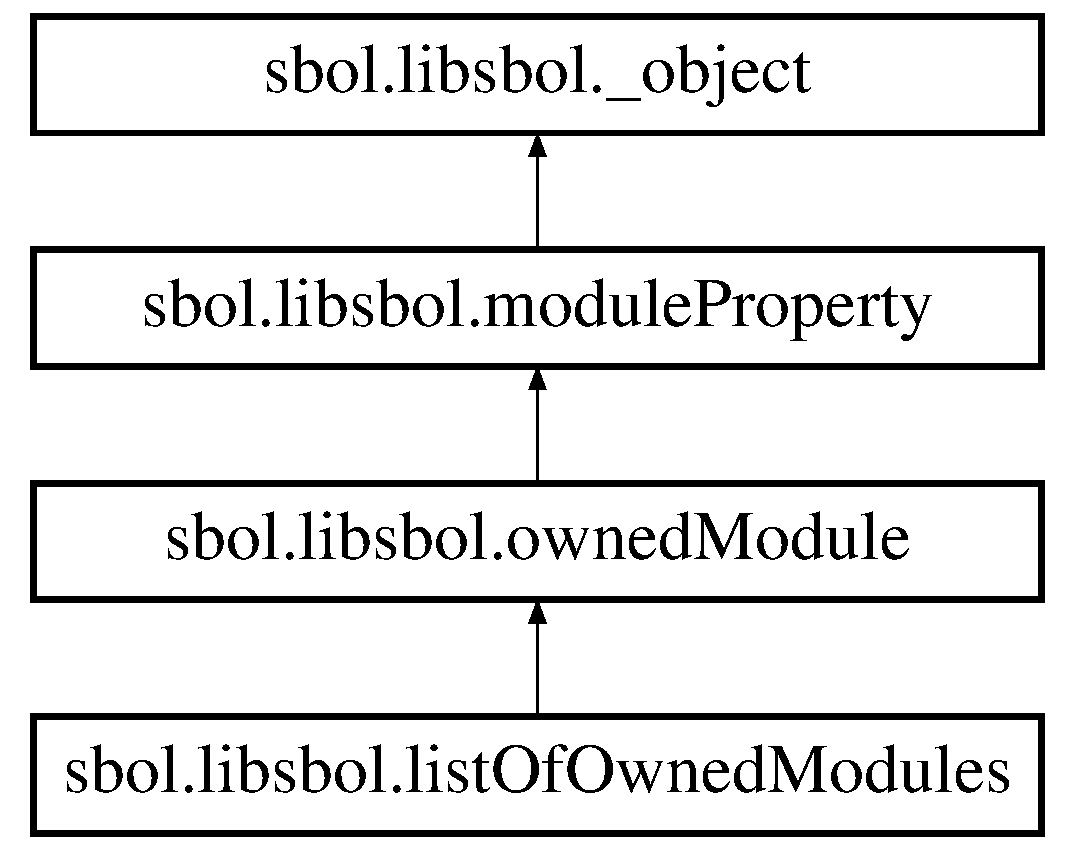
\includegraphics[height=4.000000cm]{classsbol_1_1libsbol_1_1list_of_owned_modules}
\end{center}
\end{figure}
\subsection*{Public Member Functions}
\begin{DoxyCompactItemize}
\item 
def \hyperlink{classsbol_1_1libsbol_1_1list_of_owned_modules_aa928bd17d4ecaac876d9374d1b70348a}{\+\_\+\+\_\+init\+\_\+\+\_\+} (self, args)
\item 
def \hyperlink{classsbol_1_1libsbol_1_1list_of_owned_modules_a7e5cd91ea4a288124ccf496cc933c650}{remove} (self, index)
\end{DoxyCompactItemize}
\subsection*{Public Attributes}
\begin{DoxyCompactItemize}
\item 
{\bfseries this}\hypertarget{classsbol_1_1libsbol_1_1list_of_owned_modules_a8941c5bc648934514e85ae79c6c8ef8b}{}\label{classsbol_1_1libsbol_1_1list_of_owned_modules_a8941c5bc648934514e85ae79c6c8ef8b}

\end{DoxyCompactItemize}
\subsection*{Additional Inherited Members}


\subsection{Constructor \& Destructor Documentation}
\index{sbol\+::libsbol\+::list\+Of\+Owned\+Modules@{sbol\+::libsbol\+::list\+Of\+Owned\+Modules}!\+\_\+\+\_\+init\+\_\+\+\_\+@{\+\_\+\+\_\+init\+\_\+\+\_\+}}
\index{\+\_\+\+\_\+init\+\_\+\+\_\+@{\+\_\+\+\_\+init\+\_\+\+\_\+}!sbol\+::libsbol\+::list\+Of\+Owned\+Modules@{sbol\+::libsbol\+::list\+Of\+Owned\+Modules}}
\subsubsection[{\texorpdfstring{\+\_\+\+\_\+init\+\_\+\+\_\+(self, args)}{__init__(self, args)}}]{\setlength{\rightskip}{0pt plus 5cm}def sbol.\+libsbol.\+list\+Of\+Owned\+Modules.\+\_\+\+\_\+init\+\_\+\+\_\+ (
\begin{DoxyParamCaption}
\item[{}]{self, }
\item[{}]{args}
\end{DoxyParamCaption}
)}\hypertarget{classsbol_1_1libsbol_1_1list_of_owned_modules_aa928bd17d4ecaac876d9374d1b70348a}{}\label{classsbol_1_1libsbol_1_1list_of_owned_modules_aa928bd17d4ecaac876d9374d1b70348a}
\begin{DoxyVerb}sbol::List< PropertyType
>::List(sbol_type type_uri, SBOLObject *property_owner, std::string
initial_value="") 
\end{DoxyVerb}
 

\subsection{Member Function Documentation}
\index{sbol\+::libsbol\+::list\+Of\+Owned\+Modules@{sbol\+::libsbol\+::list\+Of\+Owned\+Modules}!remove@{remove}}
\index{remove@{remove}!sbol\+::libsbol\+::list\+Of\+Owned\+Modules@{sbol\+::libsbol\+::list\+Of\+Owned\+Modules}}
\subsubsection[{\texorpdfstring{remove(self, index)}{remove(self, index)}}]{\setlength{\rightskip}{0pt plus 5cm}def sbol.\+libsbol.\+list\+Of\+Owned\+Modules.\+remove (
\begin{DoxyParamCaption}
\item[{}]{self, }
\item[{}]{index}
\end{DoxyParamCaption}
)}\hypertarget{classsbol_1_1libsbol_1_1list_of_owned_modules_a7e5cd91ea4a288124ccf496cc933c650}{}\label{classsbol_1_1libsbol_1_1list_of_owned_modules_a7e5cd91ea4a288124ccf496cc933c650}
\begin{DoxyVerb}void sbol::List<
PropertyType >::remove(int index) 
\end{DoxyVerb}
 

The documentation for this class was generated from the following file\+:\begin{DoxyCompactItemize}
\item 
libsbol.\+py\end{DoxyCompactItemize}

\hypertarget{classsbol_1_1libsbol_1_1list_of_owned_participations}{}\section{sbol.\+libsbol.\+list\+Of\+Owned\+Participations Class Reference}
\label{classsbol_1_1libsbol_1_1list_of_owned_participations}\index{sbol.\+libsbol.\+list\+Of\+Owned\+Participations@{sbol.\+libsbol.\+list\+Of\+Owned\+Participations}}
Inheritance diagram for sbol.\+libsbol.\+list\+Of\+Owned\+Participations\+:\begin{figure}[H]
\begin{center}
\leavevmode
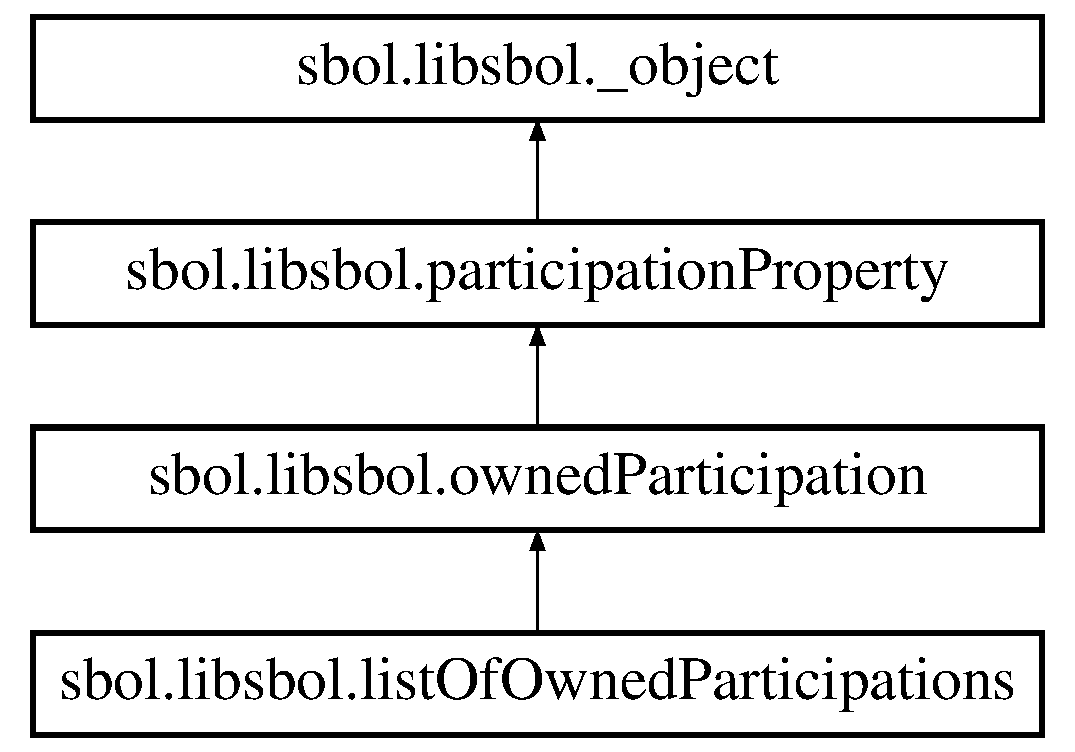
\includegraphics[height=4.000000cm]{classsbol_1_1libsbol_1_1list_of_owned_participations}
\end{center}
\end{figure}
\subsection*{Public Member Functions}
\begin{DoxyCompactItemize}
\item 
def \hyperlink{classsbol_1_1libsbol_1_1list_of_owned_participations_aaacb6cc16c8db7d85a63b1011a001e02}{\+\_\+\+\_\+init\+\_\+\+\_\+} (self, args)
\item 
def \hyperlink{classsbol_1_1libsbol_1_1list_of_owned_participations_af3aae80b15c2e4898338244cee57c75e}{remove} (self, index)
\end{DoxyCompactItemize}
\subsection*{Public Attributes}
\begin{DoxyCompactItemize}
\item 
{\bfseries this}\hypertarget{classsbol_1_1libsbol_1_1list_of_owned_participations_a00376d54c8b5d0de889a4d3d4c336427}{}\label{classsbol_1_1libsbol_1_1list_of_owned_participations_a00376d54c8b5d0de889a4d3d4c336427}

\end{DoxyCompactItemize}
\subsection*{Additional Inherited Members}


\subsection{Constructor \& Destructor Documentation}
\index{sbol\+::libsbol\+::list\+Of\+Owned\+Participations@{sbol\+::libsbol\+::list\+Of\+Owned\+Participations}!\+\_\+\+\_\+init\+\_\+\+\_\+@{\+\_\+\+\_\+init\+\_\+\+\_\+}}
\index{\+\_\+\+\_\+init\+\_\+\+\_\+@{\+\_\+\+\_\+init\+\_\+\+\_\+}!sbol\+::libsbol\+::list\+Of\+Owned\+Participations@{sbol\+::libsbol\+::list\+Of\+Owned\+Participations}}
\subsubsection[{\texorpdfstring{\+\_\+\+\_\+init\+\_\+\+\_\+(self, args)}{__init__(self, args)}}]{\setlength{\rightskip}{0pt plus 5cm}def sbol.\+libsbol.\+list\+Of\+Owned\+Participations.\+\_\+\+\_\+init\+\_\+\+\_\+ (
\begin{DoxyParamCaption}
\item[{}]{self, }
\item[{}]{args}
\end{DoxyParamCaption}
)}\hypertarget{classsbol_1_1libsbol_1_1list_of_owned_participations_aaacb6cc16c8db7d85a63b1011a001e02}{}\label{classsbol_1_1libsbol_1_1list_of_owned_participations_aaacb6cc16c8db7d85a63b1011a001e02}
\begin{DoxyVerb}sbol::List< PropertyType
>::List(sbol_type type_uri, SBOLObject *property_owner, std::string
initial_value="") 
\end{DoxyVerb}
 

\subsection{Member Function Documentation}
\index{sbol\+::libsbol\+::list\+Of\+Owned\+Participations@{sbol\+::libsbol\+::list\+Of\+Owned\+Participations}!remove@{remove}}
\index{remove@{remove}!sbol\+::libsbol\+::list\+Of\+Owned\+Participations@{sbol\+::libsbol\+::list\+Of\+Owned\+Participations}}
\subsubsection[{\texorpdfstring{remove(self, index)}{remove(self, index)}}]{\setlength{\rightskip}{0pt plus 5cm}def sbol.\+libsbol.\+list\+Of\+Owned\+Participations.\+remove (
\begin{DoxyParamCaption}
\item[{}]{self, }
\item[{}]{index}
\end{DoxyParamCaption}
)}\hypertarget{classsbol_1_1libsbol_1_1list_of_owned_participations_af3aae80b15c2e4898338244cee57c75e}{}\label{classsbol_1_1libsbol_1_1list_of_owned_participations_af3aae80b15c2e4898338244cee57c75e}
\begin{DoxyVerb}void sbol::List<
PropertyType >::remove(int index) 
\end{DoxyVerb}
 

The documentation for this class was generated from the following file\+:\begin{DoxyCompactItemize}
\item 
libsbol.\+py\end{DoxyCompactItemize}

\hypertarget{classsbol_1_1libsbol_1_1list_of_owned_sequence_annotations}{}\section{sbol.\+libsbol.\+list\+Of\+Owned\+Sequence\+Annotations Class Reference}
\label{classsbol_1_1libsbol_1_1list_of_owned_sequence_annotations}\index{sbol.\+libsbol.\+list\+Of\+Owned\+Sequence\+Annotations@{sbol.\+libsbol.\+list\+Of\+Owned\+Sequence\+Annotations}}
Inheritance diagram for sbol.\+libsbol.\+list\+Of\+Owned\+Sequence\+Annotations\+:\begin{figure}[H]
\begin{center}
\leavevmode
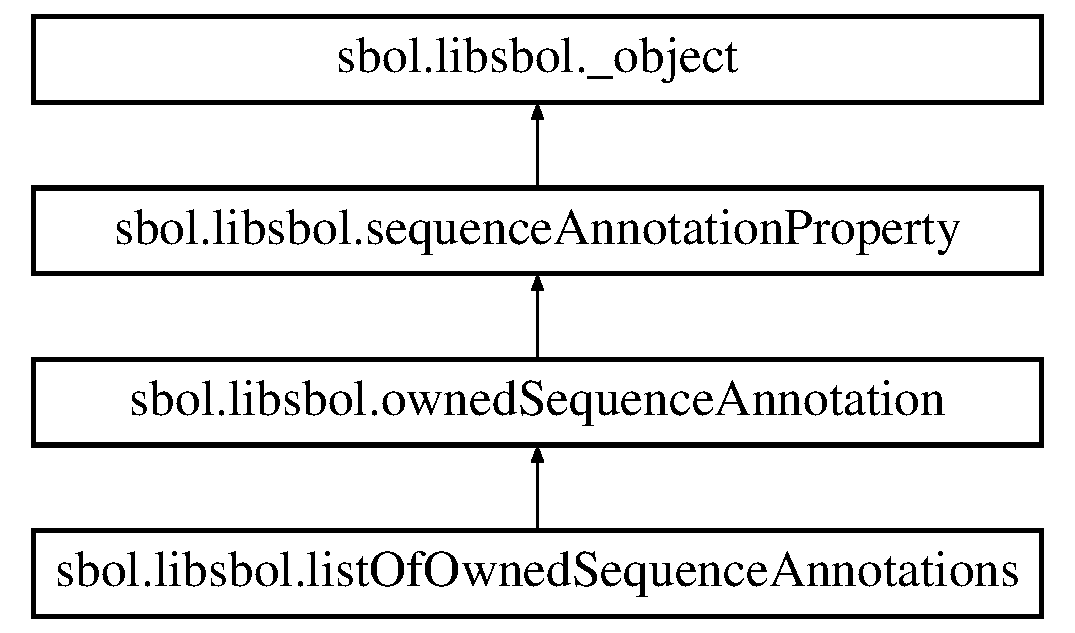
\includegraphics[height=4.000000cm]{classsbol_1_1libsbol_1_1list_of_owned_sequence_annotations}
\end{center}
\end{figure}
\subsection*{Public Member Functions}
\begin{DoxyCompactItemize}
\item 
def \hyperlink{classsbol_1_1libsbol_1_1list_of_owned_sequence_annotations_a3bfb2f31c1ff6bdeb9720b13fe490091}{\+\_\+\+\_\+init\+\_\+\+\_\+} (self, args)
\item 
def \hyperlink{classsbol_1_1libsbol_1_1list_of_owned_sequence_annotations_aa524379a36a95b187401a53e7caa2e8e}{remove} (self, index)
\end{DoxyCompactItemize}
\subsection*{Public Attributes}
\begin{DoxyCompactItemize}
\item 
{\bfseries this}\hypertarget{classsbol_1_1libsbol_1_1list_of_owned_sequence_annotations_aaad5cdee7f9eaaaed2dff21fd4b86523}{}\label{classsbol_1_1libsbol_1_1list_of_owned_sequence_annotations_aaad5cdee7f9eaaaed2dff21fd4b86523}

\end{DoxyCompactItemize}
\subsection*{Additional Inherited Members}


\subsection{Constructor \& Destructor Documentation}
\index{sbol\+::libsbol\+::list\+Of\+Owned\+Sequence\+Annotations@{sbol\+::libsbol\+::list\+Of\+Owned\+Sequence\+Annotations}!\+\_\+\+\_\+init\+\_\+\+\_\+@{\+\_\+\+\_\+init\+\_\+\+\_\+}}
\index{\+\_\+\+\_\+init\+\_\+\+\_\+@{\+\_\+\+\_\+init\+\_\+\+\_\+}!sbol\+::libsbol\+::list\+Of\+Owned\+Sequence\+Annotations@{sbol\+::libsbol\+::list\+Of\+Owned\+Sequence\+Annotations}}
\subsubsection[{\texorpdfstring{\+\_\+\+\_\+init\+\_\+\+\_\+(self, args)}{__init__(self, args)}}]{\setlength{\rightskip}{0pt plus 5cm}def sbol.\+libsbol.\+list\+Of\+Owned\+Sequence\+Annotations.\+\_\+\+\_\+init\+\_\+\+\_\+ (
\begin{DoxyParamCaption}
\item[{}]{self, }
\item[{}]{args}
\end{DoxyParamCaption}
)}\hypertarget{classsbol_1_1libsbol_1_1list_of_owned_sequence_annotations_a3bfb2f31c1ff6bdeb9720b13fe490091}{}\label{classsbol_1_1libsbol_1_1list_of_owned_sequence_annotations_a3bfb2f31c1ff6bdeb9720b13fe490091}
\begin{DoxyVerb}sbol::List< PropertyType
>::List(sbol_type type_uri, SBOLObject *property_owner, std::string
initial_value="") 
\end{DoxyVerb}
 

\subsection{Member Function Documentation}
\index{sbol\+::libsbol\+::list\+Of\+Owned\+Sequence\+Annotations@{sbol\+::libsbol\+::list\+Of\+Owned\+Sequence\+Annotations}!remove@{remove}}
\index{remove@{remove}!sbol\+::libsbol\+::list\+Of\+Owned\+Sequence\+Annotations@{sbol\+::libsbol\+::list\+Of\+Owned\+Sequence\+Annotations}}
\subsubsection[{\texorpdfstring{remove(self, index)}{remove(self, index)}}]{\setlength{\rightskip}{0pt plus 5cm}def sbol.\+libsbol.\+list\+Of\+Owned\+Sequence\+Annotations.\+remove (
\begin{DoxyParamCaption}
\item[{}]{self, }
\item[{}]{index}
\end{DoxyParamCaption}
)}\hypertarget{classsbol_1_1libsbol_1_1list_of_owned_sequence_annotations_aa524379a36a95b187401a53e7caa2e8e}{}\label{classsbol_1_1libsbol_1_1list_of_owned_sequence_annotations_aa524379a36a95b187401a53e7caa2e8e}
\begin{DoxyVerb}void sbol::List<
PropertyType >::remove(int index) 
\end{DoxyVerb}
 

The documentation for this class was generated from the following file\+:\begin{DoxyCompactItemize}
\item 
libsbol.\+py\end{DoxyCompactItemize}

\hypertarget{classsbol_1_1libsbol_1_1list_of_owned_sequence_constraints}{}\section{sbol.\+libsbol.\+list\+Of\+Owned\+Sequence\+Constraints Class Reference}
\label{classsbol_1_1libsbol_1_1list_of_owned_sequence_constraints}\index{sbol.\+libsbol.\+list\+Of\+Owned\+Sequence\+Constraints@{sbol.\+libsbol.\+list\+Of\+Owned\+Sequence\+Constraints}}
Inheritance diagram for sbol.\+libsbol.\+list\+Of\+Owned\+Sequence\+Constraints\+:\begin{figure}[H]
\begin{center}
\leavevmode
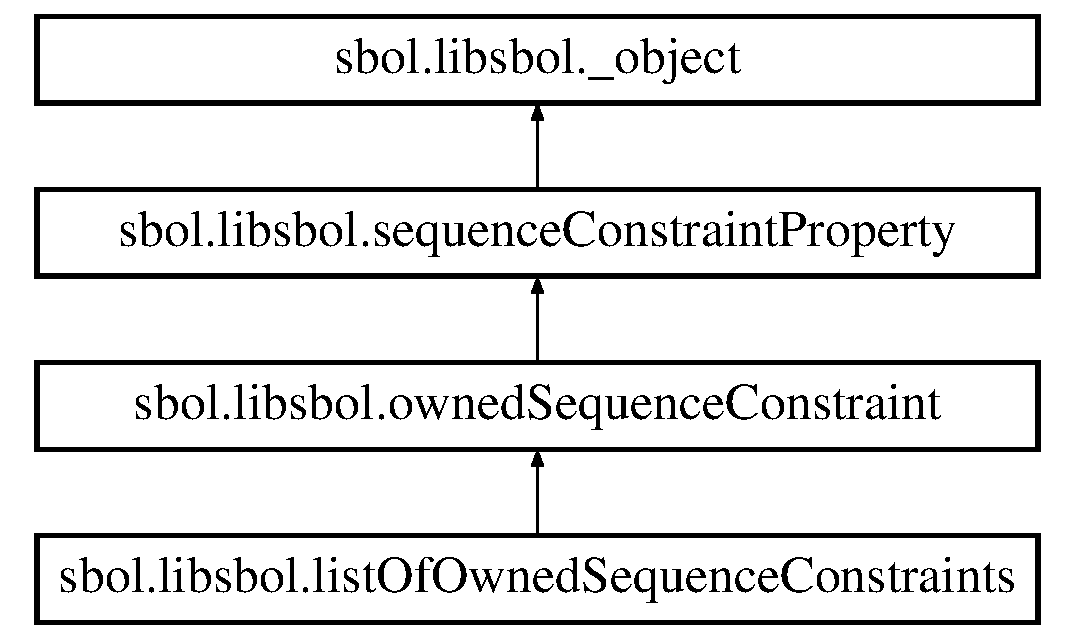
\includegraphics[height=4.000000cm]{classsbol_1_1libsbol_1_1list_of_owned_sequence_constraints}
\end{center}
\end{figure}
\subsection*{Public Member Functions}
\begin{DoxyCompactItemize}
\item 
def \hyperlink{classsbol_1_1libsbol_1_1list_of_owned_sequence_constraints_a81ff041e1d7ad199ec6fd6f15e3fad71}{\+\_\+\+\_\+init\+\_\+\+\_\+} (self, args)
\item 
def \hyperlink{classsbol_1_1libsbol_1_1list_of_owned_sequence_constraints_a795739ab5b53c119ec54998a517624b0}{remove} (self, index)
\end{DoxyCompactItemize}
\subsection*{Public Attributes}
\begin{DoxyCompactItemize}
\item 
{\bfseries this}\hypertarget{classsbol_1_1libsbol_1_1list_of_owned_sequence_constraints_a5684d5bffaf2217e755d44bbb45757be}{}\label{classsbol_1_1libsbol_1_1list_of_owned_sequence_constraints_a5684d5bffaf2217e755d44bbb45757be}

\end{DoxyCompactItemize}
\subsection*{Additional Inherited Members}


\subsection{Constructor \& Destructor Documentation}
\index{sbol\+::libsbol\+::list\+Of\+Owned\+Sequence\+Constraints@{sbol\+::libsbol\+::list\+Of\+Owned\+Sequence\+Constraints}!\+\_\+\+\_\+init\+\_\+\+\_\+@{\+\_\+\+\_\+init\+\_\+\+\_\+}}
\index{\+\_\+\+\_\+init\+\_\+\+\_\+@{\+\_\+\+\_\+init\+\_\+\+\_\+}!sbol\+::libsbol\+::list\+Of\+Owned\+Sequence\+Constraints@{sbol\+::libsbol\+::list\+Of\+Owned\+Sequence\+Constraints}}
\subsubsection[{\texorpdfstring{\+\_\+\+\_\+init\+\_\+\+\_\+(self, args)}{__init__(self, args)}}]{\setlength{\rightskip}{0pt plus 5cm}def sbol.\+libsbol.\+list\+Of\+Owned\+Sequence\+Constraints.\+\_\+\+\_\+init\+\_\+\+\_\+ (
\begin{DoxyParamCaption}
\item[{}]{self, }
\item[{}]{args}
\end{DoxyParamCaption}
)}\hypertarget{classsbol_1_1libsbol_1_1list_of_owned_sequence_constraints_a81ff041e1d7ad199ec6fd6f15e3fad71}{}\label{classsbol_1_1libsbol_1_1list_of_owned_sequence_constraints_a81ff041e1d7ad199ec6fd6f15e3fad71}
\begin{DoxyVerb}sbol::List< PropertyType
>::List(sbol_type type_uri, SBOLObject *property_owner, std::string
initial_value="") 
\end{DoxyVerb}
 

\subsection{Member Function Documentation}
\index{sbol\+::libsbol\+::list\+Of\+Owned\+Sequence\+Constraints@{sbol\+::libsbol\+::list\+Of\+Owned\+Sequence\+Constraints}!remove@{remove}}
\index{remove@{remove}!sbol\+::libsbol\+::list\+Of\+Owned\+Sequence\+Constraints@{sbol\+::libsbol\+::list\+Of\+Owned\+Sequence\+Constraints}}
\subsubsection[{\texorpdfstring{remove(self, index)}{remove(self, index)}}]{\setlength{\rightskip}{0pt plus 5cm}def sbol.\+libsbol.\+list\+Of\+Owned\+Sequence\+Constraints.\+remove (
\begin{DoxyParamCaption}
\item[{}]{self, }
\item[{}]{index}
\end{DoxyParamCaption}
)}\hypertarget{classsbol_1_1libsbol_1_1list_of_owned_sequence_constraints_a795739ab5b53c119ec54998a517624b0}{}\label{classsbol_1_1libsbol_1_1list_of_owned_sequence_constraints_a795739ab5b53c119ec54998a517624b0}
\begin{DoxyVerb}void sbol::List<
PropertyType >::remove(int index) 
\end{DoxyVerb}
 

The documentation for this class was generated from the following file\+:\begin{DoxyCompactItemize}
\item 
libsbol.\+py\end{DoxyCompactItemize}

\hypertarget{classsbol_1_1libsbol_1_1list_of_u_r_is}{}\section{sbol.\+libsbol.\+list\+Of\+U\+R\+Is Class Reference}
\label{classsbol_1_1libsbol_1_1list_of_u_r_is}\index{sbol.\+libsbol.\+list\+Of\+U\+R\+Is@{sbol.\+libsbol.\+list\+Of\+U\+R\+Is}}
Inheritance diagram for sbol.\+libsbol.\+list\+Of\+U\+R\+Is\+:\begin{figure}[H]
\begin{center}
\leavevmode
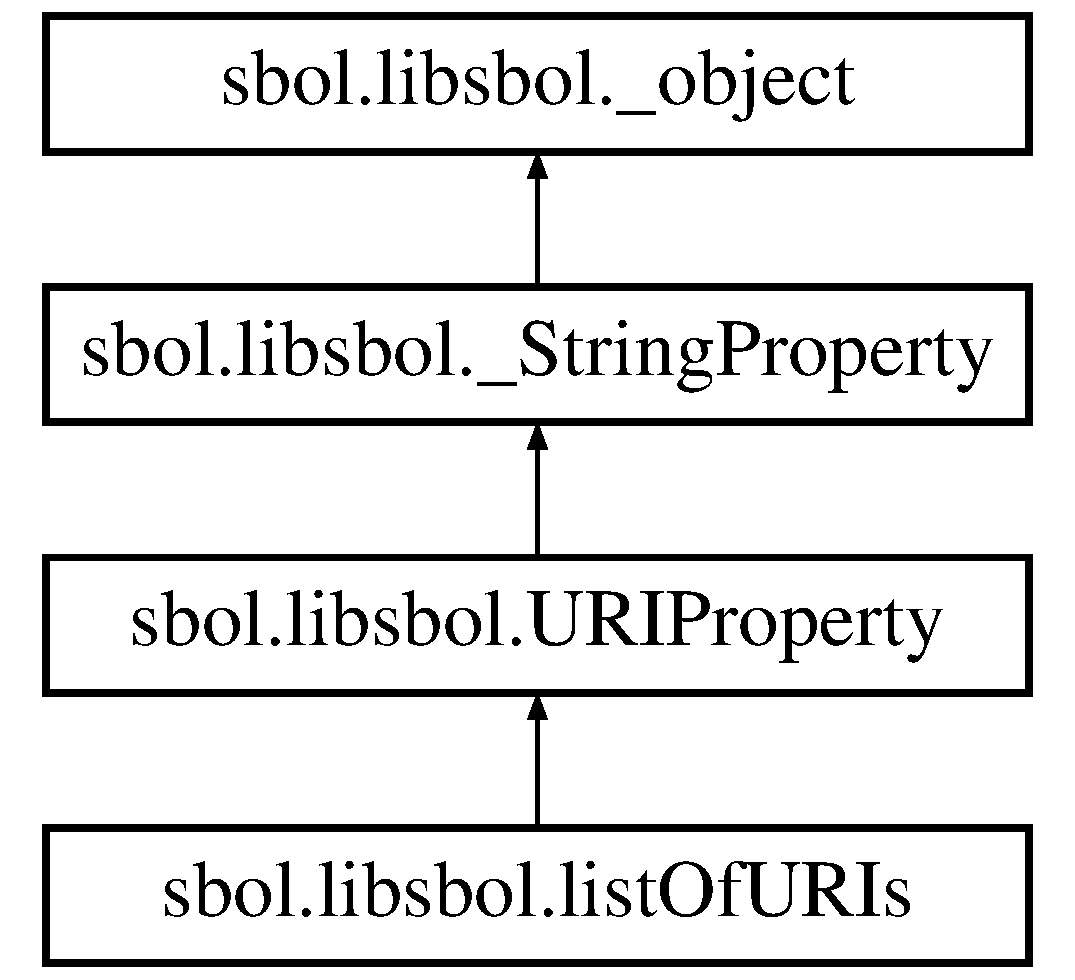
\includegraphics[height=4.000000cm]{classsbol_1_1libsbol_1_1list_of_u_r_is}
\end{center}
\end{figure}
\subsection*{Public Member Functions}
\begin{DoxyCompactItemize}
\item 
def \hyperlink{classsbol_1_1libsbol_1_1list_of_u_r_is_a9626dd3518333f683a3fcd84e9afffef}{\+\_\+\+\_\+init\+\_\+\+\_\+} (self, args)
\item 
def \hyperlink{classsbol_1_1libsbol_1_1list_of_u_r_is_ac413a59cfe08b95c62c8809ad75467dc}{remove} (self, index)
\end{DoxyCompactItemize}
\subsection*{Public Attributes}
\begin{DoxyCompactItemize}
\item 
{\bfseries this}\hypertarget{classsbol_1_1libsbol_1_1list_of_u_r_is_a9cb6b5694ea34e3b2da23da8ede10b3e}{}\label{classsbol_1_1libsbol_1_1list_of_u_r_is_a9cb6b5694ea34e3b2da23da8ede10b3e}

\end{DoxyCompactItemize}


\subsection{Constructor \& Destructor Documentation}
\index{sbol\+::libsbol\+::list\+Of\+U\+R\+Is@{sbol\+::libsbol\+::list\+Of\+U\+R\+Is}!\+\_\+\+\_\+init\+\_\+\+\_\+@{\+\_\+\+\_\+init\+\_\+\+\_\+}}
\index{\+\_\+\+\_\+init\+\_\+\+\_\+@{\+\_\+\+\_\+init\+\_\+\+\_\+}!sbol\+::libsbol\+::list\+Of\+U\+R\+Is@{sbol\+::libsbol\+::list\+Of\+U\+R\+Is}}
\subsubsection[{\texorpdfstring{\+\_\+\+\_\+init\+\_\+\+\_\+(self, args)}{__init__(self, args)}}]{\setlength{\rightskip}{0pt plus 5cm}def sbol.\+libsbol.\+list\+Of\+U\+R\+Is.\+\_\+\+\_\+init\+\_\+\+\_\+ (
\begin{DoxyParamCaption}
\item[{}]{self, }
\item[{}]{args}
\end{DoxyParamCaption}
)}\hypertarget{classsbol_1_1libsbol_1_1list_of_u_r_is_a9626dd3518333f683a3fcd84e9afffef}{}\label{classsbol_1_1libsbol_1_1list_of_u_r_is_a9626dd3518333f683a3fcd84e9afffef}
\begin{DoxyVerb}sbol::List< PropertyType
>::List(sbol_type type_uri, SBOLObject *property_owner, std::string
initial_value="") 
\end{DoxyVerb}
 

\subsection{Member Function Documentation}
\index{sbol\+::libsbol\+::list\+Of\+U\+R\+Is@{sbol\+::libsbol\+::list\+Of\+U\+R\+Is}!remove@{remove}}
\index{remove@{remove}!sbol\+::libsbol\+::list\+Of\+U\+R\+Is@{sbol\+::libsbol\+::list\+Of\+U\+R\+Is}}
\subsubsection[{\texorpdfstring{remove(self, index)}{remove(self, index)}}]{\setlength{\rightskip}{0pt plus 5cm}def sbol.\+libsbol.\+list\+Of\+U\+R\+Is.\+remove (
\begin{DoxyParamCaption}
\item[{}]{self, }
\item[{}]{index}
\end{DoxyParamCaption}
)}\hypertarget{classsbol_1_1libsbol_1_1list_of_u_r_is_ac413a59cfe08b95c62c8809ad75467dc}{}\label{classsbol_1_1libsbol_1_1list_of_u_r_is_ac413a59cfe08b95c62c8809ad75467dc}
\begin{DoxyVerb}void sbol::List<
PropertyType >::remove(int index) 
\end{DoxyVerb}
 

The documentation for this class was generated from the following file\+:\begin{DoxyCompactItemize}
\item 
libsbol.\+py\end{DoxyCompactItemize}

\hypertarget{classsbol_1_1libsbol_1_1_location}{}\section{sbol.\+libsbol.\+Location Class Reference}
\label{classsbol_1_1libsbol_1_1_location}\index{sbol.\+libsbol.\+Location@{sbol.\+libsbol.\+Location}}
Inheritance diagram for sbol.\+libsbol.\+Location\+:\begin{figure}[H]
\begin{center}
\leavevmode
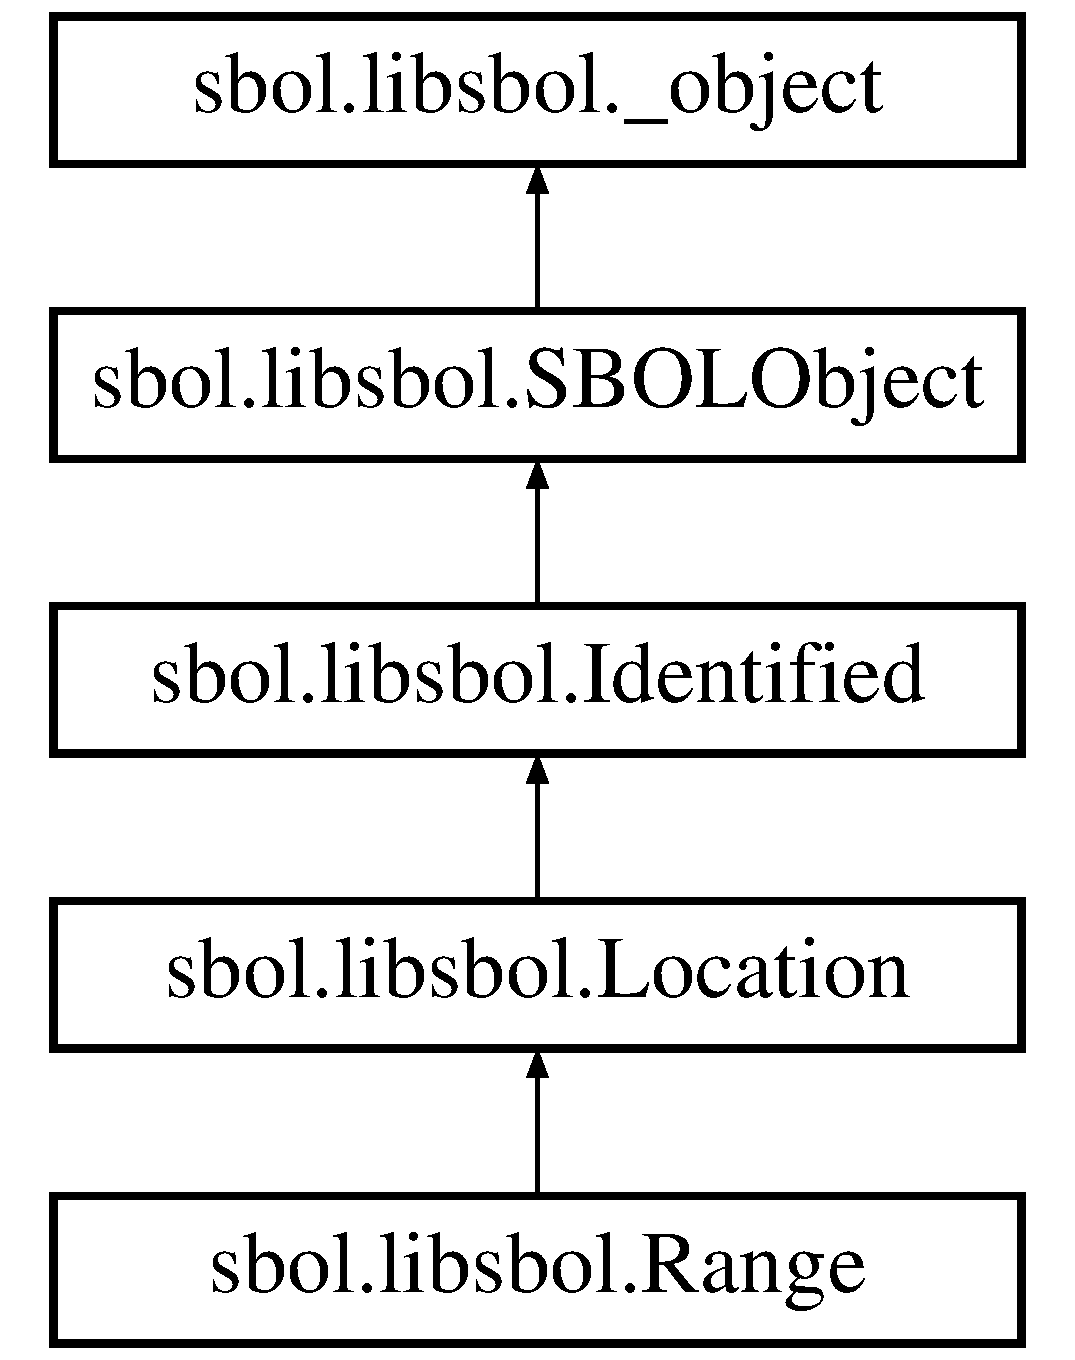
\includegraphics[height=5.000000cm]{classsbol_1_1libsbol_1_1_location}
\end{center}
\end{figure}
\subsection*{Public Member Functions}
\begin{DoxyCompactItemize}
\item 
def \hyperlink{classsbol_1_1libsbol_1_1_location_ad7951e052a7ad74601e2b1ecf72085b0}{\+\_\+\+\_\+init\+\_\+\+\_\+} (self, args)
\end{DoxyCompactItemize}
\subsection*{Public Attributes}
\begin{DoxyCompactItemize}
\item 
{\bfseries this}\hypertarget{classsbol_1_1libsbol_1_1_location_acc6f8f53e3d4a40163b4b08b7259d9d7}{}\label{classsbol_1_1libsbol_1_1_location_acc6f8f53e3d4a40163b4b08b7259d9d7}

\end{DoxyCompactItemize}
\subsection*{Static Public Attributes}
\begin{DoxyCompactItemize}
\item 
{\bfseries orientation} = \+\_\+swig\+\_\+property(\+\_\+libsbol.\+Location\+\_\+orientation\+\_\+get, \+\_\+libsbol.\+Location\+\_\+orientation\+\_\+set)\hypertarget{classsbol_1_1libsbol_1_1_location_a69b3ce1b30ffeb03a18b2a1e07c0e7c6}{}\label{classsbol_1_1libsbol_1_1_location_a69b3ce1b30ffeb03a18b2a1e07c0e7c6}

\end{DoxyCompactItemize}


\subsection{Constructor \& Destructor Documentation}
\index{sbol\+::libsbol\+::\+Location@{sbol\+::libsbol\+::\+Location}!\+\_\+\+\_\+init\+\_\+\+\_\+@{\+\_\+\+\_\+init\+\_\+\+\_\+}}
\index{\+\_\+\+\_\+init\+\_\+\+\_\+@{\+\_\+\+\_\+init\+\_\+\+\_\+}!sbol\+::libsbol\+::\+Location@{sbol\+::libsbol\+::\+Location}}
\subsubsection[{\texorpdfstring{\+\_\+\+\_\+init\+\_\+\+\_\+(self, args)}{__init__(self, args)}}]{\setlength{\rightskip}{0pt plus 5cm}def sbol.\+libsbol.\+Location.\+\_\+\+\_\+init\+\_\+\+\_\+ (
\begin{DoxyParamCaption}
\item[{}]{self, }
\item[{}]{args}
\end{DoxyParamCaption}
)}\hypertarget{classsbol_1_1libsbol_1_1_location_ad7951e052a7ad74601e2b1ecf72085b0}{}\label{classsbol_1_1libsbol_1_1_location_ad7951e052a7ad74601e2b1ecf72085b0}
\begin{DoxyVerb}sbol::Location::Location(sbol_type, std::string uri_prefix,
std::string display_id, std::string version) 
\end{DoxyVerb}
 

The documentation for this class was generated from the following file\+:\begin{DoxyCompactItemize}
\item 
libsbol.\+py\end{DoxyCompactItemize}

\hypertarget{classsbol_1_1libsbol_1_1location_property}{}\section{sbol.\+libsbol.\+location\+Property Class Reference}
\label{classsbol_1_1libsbol_1_1location_property}\index{sbol.\+libsbol.\+location\+Property@{sbol.\+libsbol.\+location\+Property}}
Inheritance diagram for sbol.\+libsbol.\+location\+Property\+:\begin{figure}[H]
\begin{center}
\leavevmode
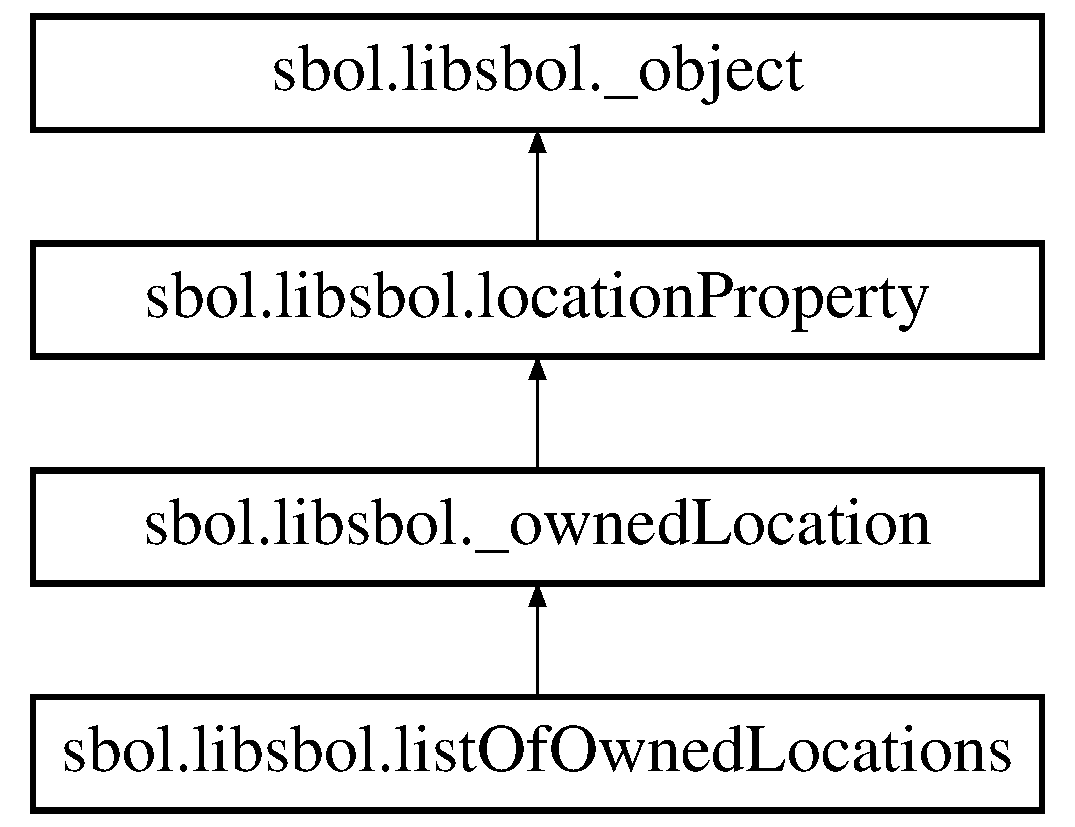
\includegraphics[height=4.000000cm]{classsbol_1_1libsbol_1_1location_property}
\end{center}
\end{figure}
\subsection*{Public Member Functions}
\begin{DoxyCompactItemize}
\item 
def \hyperlink{classsbol_1_1libsbol_1_1location_property_aeaececeda9f0c5b56f99381bcecb3b77}{\+\_\+\+\_\+init\+\_\+\+\_\+} (self, args)
\item 
def \hyperlink{classsbol_1_1libsbol_1_1location_property_ac0a184bbb7fba88bc614bf638435c16d}{get\+Type\+U\+RI} (self)
\item 
def \hyperlink{classsbol_1_1libsbol_1_1location_property_a557232b6174dfb9cde4600a5dc2313c1}{get\+Owner} (self)
\item 
def \hyperlink{classsbol_1_1libsbol_1_1location_property_a9579f64f1ae431d76c7064b91a8a8d9a}{get} (self)
\item 
def \hyperlink{classsbol_1_1libsbol_1_1location_property_ab29ffb0c8cda0185fd7f89d06fbaca84}{add} (self, new\+\_\+value)
\item 
def \hyperlink{classsbol_1_1libsbol_1_1location_property_abd3a502bca73a7b24aa8f4c5c93a211c}{set} (self, args)
\item 
def \hyperlink{classsbol_1_1libsbol_1_1location_property_acb1636639d1a450e854d83d3f08e3722}{write} (self)
\item 
def \hyperlink{classsbol_1_1libsbol_1_1location_property_a9dd8b733d0d78f17136a6a74565719ac}{validate} (self, arg=None)
\item 
def {\bfseries \+\_\+\+\_\+getitem\+\_\+\+\_\+} (self, n\+Index)\hypertarget{classsbol_1_1libsbol_1_1location_property_a1dff12083870ca55160a55515861bd33}{}\label{classsbol_1_1libsbol_1_1location_property_a1dff12083870ca55160a55515861bd33}

\item 
def {\bfseries \+\_\+\+\_\+iter\+\_\+\+\_\+} (self)\hypertarget{classsbol_1_1libsbol_1_1location_property_a65450e75956de785a296e2e5bd934cb7}{}\label{classsbol_1_1libsbol_1_1location_property_a65450e75956de785a296e2e5bd934cb7}

\item 
def {\bfseries next} (self)\hypertarget{classsbol_1_1libsbol_1_1location_property_ad3fd9bc4b51825c39a098573990766be}{}\label{classsbol_1_1libsbol_1_1location_property_ad3fd9bc4b51825c39a098573990766be}

\item 
def {\bfseries \+\_\+\+\_\+len\+\_\+\+\_\+} (self)\hypertarget{classsbol_1_1libsbol_1_1location_property_a7f1c8491d6a5ecdf38f23119dd8f2e5d}{}\label{classsbol_1_1libsbol_1_1location_property_a7f1c8491d6a5ecdf38f23119dd8f2e5d}

\end{DoxyCompactItemize}
\subsection*{Public Attributes}
\begin{DoxyCompactItemize}
\item 
{\bfseries this}\hypertarget{classsbol_1_1libsbol_1_1location_property_acc78718a7c8464d9379444b1546f4724}{}\label{classsbol_1_1libsbol_1_1location_property_acc78718a7c8464d9379444b1546f4724}

\end{DoxyCompactItemize}


\subsection{Detailed Description}
\begin{DoxyVerb}metafunction for generation of a map of message types to their
associated callbacks.

Usage: Use generate_callback_map<Type>::type to ...

Parameters:
-----------

LiteralType:  The library currently supports Property<string> and
Property<int> specification currently supports integer, string, and
URI literals

C++ includes: property.h 
\end{DoxyVerb}
 

\subsection{Constructor \& Destructor Documentation}
\index{sbol\+::libsbol\+::location\+Property@{sbol\+::libsbol\+::location\+Property}!\+\_\+\+\_\+init\+\_\+\+\_\+@{\+\_\+\+\_\+init\+\_\+\+\_\+}}
\index{\+\_\+\+\_\+init\+\_\+\+\_\+@{\+\_\+\+\_\+init\+\_\+\+\_\+}!sbol\+::libsbol\+::location\+Property@{sbol\+::libsbol\+::location\+Property}}
\subsubsection[{\texorpdfstring{\+\_\+\+\_\+init\+\_\+\+\_\+(self, args)}{__init__(self, args)}}]{\setlength{\rightskip}{0pt plus 5cm}def sbol.\+libsbol.\+location\+Property.\+\_\+\+\_\+init\+\_\+\+\_\+ (
\begin{DoxyParamCaption}
\item[{}]{self, }
\item[{}]{args}
\end{DoxyParamCaption}
)}\hypertarget{classsbol_1_1libsbol_1_1location_property_aeaececeda9f0c5b56f99381bcecb3b77}{}\label{classsbol_1_1libsbol_1_1location_property_aeaececeda9f0c5b56f99381bcecb3b77}
\begin{DoxyVerb}sbol::Property<
LiteralType >::Property(sbol_type type_uri=UNDEFINED, void
*property_owner=NULL, ValidationRules validation_rules={}) 
\end{DoxyVerb}
 

\subsection{Member Function Documentation}
\index{sbol\+::libsbol\+::location\+Property@{sbol\+::libsbol\+::location\+Property}!add@{add}}
\index{add@{add}!sbol\+::libsbol\+::location\+Property@{sbol\+::libsbol\+::location\+Property}}
\subsubsection[{\texorpdfstring{add(self, new\+\_\+value)}{add(self, new_value)}}]{\setlength{\rightskip}{0pt plus 5cm}def sbol.\+libsbol.\+location\+Property.\+add (
\begin{DoxyParamCaption}
\item[{}]{self, }
\item[{}]{new\+\_\+value}
\end{DoxyParamCaption}
)}\hypertarget{classsbol_1_1libsbol_1_1location_property_ab29ffb0c8cda0185fd7f89d06fbaca84}{}\label{classsbol_1_1libsbol_1_1location_property_ab29ffb0c8cda0185fd7f89d06fbaca84}
\begin{DoxyVerb}void sbol::Property<
LiteralType >::add(std::string new_value) 
\end{DoxyVerb}
 \index{sbol\+::libsbol\+::location\+Property@{sbol\+::libsbol\+::location\+Property}!get@{get}}
\index{get@{get}!sbol\+::libsbol\+::location\+Property@{sbol\+::libsbol\+::location\+Property}}
\subsubsection[{\texorpdfstring{get(self)}{get(self)}}]{\setlength{\rightskip}{0pt plus 5cm}def sbol.\+libsbol.\+location\+Property.\+get (
\begin{DoxyParamCaption}
\item[{}]{self}
\end{DoxyParamCaption}
)}\hypertarget{classsbol_1_1libsbol_1_1location_property_a9579f64f1ae431d76c7064b91a8a8d9a}{}\label{classsbol_1_1libsbol_1_1location_property_a9579f64f1ae431d76c7064b91a8a8d9a}
\begin{DoxyVerb}std::string
sbol::Property< LiteralType >::get() 
\end{DoxyVerb}
 \index{sbol\+::libsbol\+::location\+Property@{sbol\+::libsbol\+::location\+Property}!get\+Owner@{get\+Owner}}
\index{get\+Owner@{get\+Owner}!sbol\+::libsbol\+::location\+Property@{sbol\+::libsbol\+::location\+Property}}
\subsubsection[{\texorpdfstring{get\+Owner(self)}{getOwner(self)}}]{\setlength{\rightskip}{0pt plus 5cm}def sbol.\+libsbol.\+location\+Property.\+get\+Owner (
\begin{DoxyParamCaption}
\item[{}]{self}
\end{DoxyParamCaption}
)}\hypertarget{classsbol_1_1libsbol_1_1location_property_a557232b6174dfb9cde4600a5dc2313c1}{}\label{classsbol_1_1libsbol_1_1location_property_a557232b6174dfb9cde4600a5dc2313c1}
\begin{DoxyVerb}SBOLObject &
sbol::Property< LiteralType >::getOwner() 
\end{DoxyVerb}
 \index{sbol\+::libsbol\+::location\+Property@{sbol\+::libsbol\+::location\+Property}!get\+Type\+U\+RI@{get\+Type\+U\+RI}}
\index{get\+Type\+U\+RI@{get\+Type\+U\+RI}!sbol\+::libsbol\+::location\+Property@{sbol\+::libsbol\+::location\+Property}}
\subsubsection[{\texorpdfstring{get\+Type\+U\+R\+I(self)}{getTypeURI(self)}}]{\setlength{\rightskip}{0pt plus 5cm}def sbol.\+libsbol.\+location\+Property.\+get\+Type\+U\+RI (
\begin{DoxyParamCaption}
\item[{}]{self}
\end{DoxyParamCaption}
)}\hypertarget{classsbol_1_1libsbol_1_1location_property_ac0a184bbb7fba88bc614bf638435c16d}{}\label{classsbol_1_1libsbol_1_1location_property_ac0a184bbb7fba88bc614bf638435c16d}
\begin{DoxyVerb}sbol_type
sbol::Property< LiteralType >::getTypeURI() 
\end{DoxyVerb}
 \index{sbol\+::libsbol\+::location\+Property@{sbol\+::libsbol\+::location\+Property}!set@{set}}
\index{set@{set}!sbol\+::libsbol\+::location\+Property@{sbol\+::libsbol\+::location\+Property}}
\subsubsection[{\texorpdfstring{set(self, args)}{set(self, args)}}]{\setlength{\rightskip}{0pt plus 5cm}def sbol.\+libsbol.\+location\+Property.\+set (
\begin{DoxyParamCaption}
\item[{}]{self, }
\item[{}]{args}
\end{DoxyParamCaption}
)}\hypertarget{classsbol_1_1libsbol_1_1location_property_abd3a502bca73a7b24aa8f4c5c93a211c}{}\label{classsbol_1_1libsbol_1_1location_property_abd3a502bca73a7b24aa8f4c5c93a211c}
\begin{DoxyVerb}void sbol::Property<
LiteralType >::set(int new_value) 
\end{DoxyVerb}
 \index{sbol\+::libsbol\+::location\+Property@{sbol\+::libsbol\+::location\+Property}!validate@{validate}}
\index{validate@{validate}!sbol\+::libsbol\+::location\+Property@{sbol\+::libsbol\+::location\+Property}}
\subsubsection[{\texorpdfstring{validate(self, arg=\+None)}{validate(self, arg=None)}}]{\setlength{\rightskip}{0pt plus 5cm}def sbol.\+libsbol.\+location\+Property.\+validate (
\begin{DoxyParamCaption}
\item[{}]{self, }
\item[{}]{arg = {\ttfamily None}}
\end{DoxyParamCaption}
)}\hypertarget{classsbol_1_1libsbol_1_1location_property_a9dd8b733d0d78f17136a6a74565719ac}{}\label{classsbol_1_1libsbol_1_1location_property_a9dd8b733d0d78f17136a6a74565719ac}
\begin{DoxyVerb}void sbol::Property<
LiteralType >::validate(void *arg=NULL) 
\end{DoxyVerb}
 \index{sbol\+::libsbol\+::location\+Property@{sbol\+::libsbol\+::location\+Property}!write@{write}}
\index{write@{write}!sbol\+::libsbol\+::location\+Property@{sbol\+::libsbol\+::location\+Property}}
\subsubsection[{\texorpdfstring{write(self)}{write(self)}}]{\setlength{\rightskip}{0pt plus 5cm}def sbol.\+libsbol.\+location\+Property.\+write (
\begin{DoxyParamCaption}
\item[{}]{self}
\end{DoxyParamCaption}
)}\hypertarget{classsbol_1_1libsbol_1_1location_property_acb1636639d1a450e854d83d3f08e3722}{}\label{classsbol_1_1libsbol_1_1location_property_acb1636639d1a450e854d83d3f08e3722}
\begin{DoxyVerb}void sbol::Property<
LiteralType >::write() 
\end{DoxyVerb}
 

The documentation for this class was generated from the following file\+:\begin{DoxyCompactItemize}
\item 
libsbol.\+py\end{DoxyCompactItemize}

\hypertarget{classsbol_1_1libsbol_1_1_maps_to}{}\section{sbol.\+libsbol.\+Maps\+To Class Reference}
\label{classsbol_1_1libsbol_1_1_maps_to}\index{sbol.\+libsbol.\+Maps\+To@{sbol.\+libsbol.\+Maps\+To}}
Inheritance diagram for sbol.\+libsbol.\+Maps\+To\+:\begin{figure}[H]
\begin{center}
\leavevmode
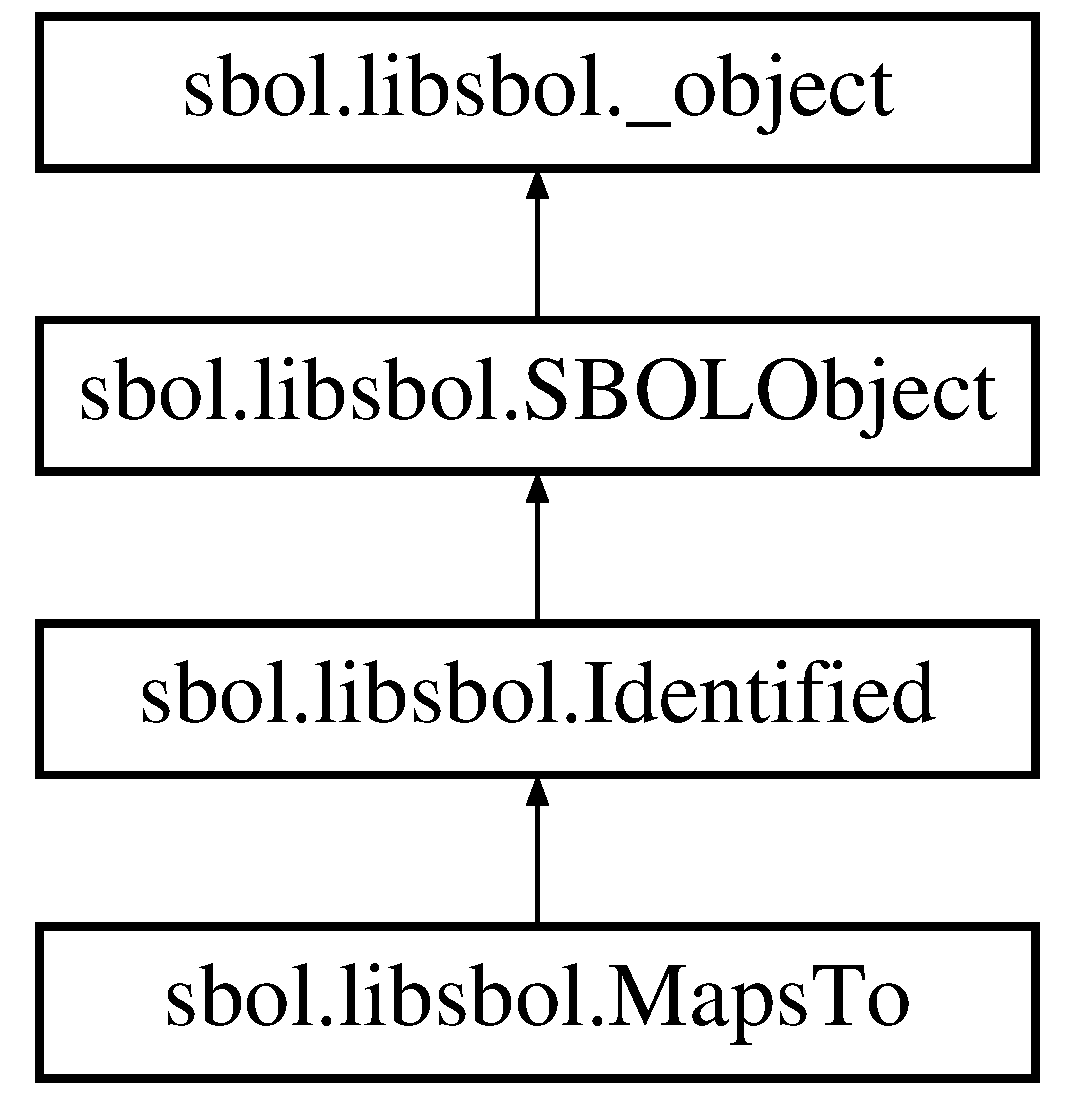
\includegraphics[height=4.000000cm]{classsbol_1_1libsbol_1_1_maps_to}
\end{center}
\end{figure}
\subsection*{Public Member Functions}
\begin{DoxyCompactItemize}
\item 
def \hyperlink{classsbol_1_1libsbol_1_1_maps_to_a86cb474078deafb4da5ee28ce43c5a10}{\+\_\+\+\_\+init\+\_\+\+\_\+} (self, args)
\end{DoxyCompactItemize}
\subsection*{Public Attributes}
\begin{DoxyCompactItemize}
\item 
{\bfseries this}\hypertarget{classsbol_1_1libsbol_1_1_maps_to_a1669f9e878853c6cd190a58a443dc35d}{}\label{classsbol_1_1libsbol_1_1_maps_to_a1669f9e878853c6cd190a58a443dc35d}

\end{DoxyCompactItemize}
\subsection*{Static Public Attributes}
\begin{DoxyCompactItemize}
\item 
{\bfseries refinement} = \+\_\+swig\+\_\+property(\+\_\+libsbol.\+Maps\+To\+\_\+refinement\+\_\+get, \+\_\+libsbol.\+Maps\+To\+\_\+refinement\+\_\+set)\hypertarget{classsbol_1_1libsbol_1_1_maps_to_a8d107d0ebfbaed04a348d66f1d6d6ed9}{}\label{classsbol_1_1libsbol_1_1_maps_to_a8d107d0ebfbaed04a348d66f1d6d6ed9}

\item 
{\bfseries local} = \+\_\+swig\+\_\+property(\+\_\+libsbol.\+Maps\+To\+\_\+local\+\_\+get, \+\_\+libsbol.\+Maps\+To\+\_\+local\+\_\+set)\hypertarget{classsbol_1_1libsbol_1_1_maps_to_a6b767b5b1ad5a49a00d2f3b1e3c51a1a}{}\label{classsbol_1_1libsbol_1_1_maps_to_a6b767b5b1ad5a49a00d2f3b1e3c51a1a}

\item 
{\bfseries remote} = \+\_\+swig\+\_\+property(\+\_\+libsbol.\+Maps\+To\+\_\+remote\+\_\+get, \+\_\+libsbol.\+Maps\+To\+\_\+remote\+\_\+set)\hypertarget{classsbol_1_1libsbol_1_1_maps_to_ac0ea38dce87cacb5154999021fc8973e}{}\label{classsbol_1_1libsbol_1_1_maps_to_ac0ea38dce87cacb5154999021fc8973e}

\end{DoxyCompactItemize}


\subsection{Constructor \& Destructor Documentation}
\index{sbol\+::libsbol\+::\+Maps\+To@{sbol\+::libsbol\+::\+Maps\+To}!\+\_\+\+\_\+init\+\_\+\+\_\+@{\+\_\+\+\_\+init\+\_\+\+\_\+}}
\index{\+\_\+\+\_\+init\+\_\+\+\_\+@{\+\_\+\+\_\+init\+\_\+\+\_\+}!sbol\+::libsbol\+::\+Maps\+To@{sbol\+::libsbol\+::\+Maps\+To}}
\subsubsection[{\texorpdfstring{\+\_\+\+\_\+init\+\_\+\+\_\+(self, args)}{__init__(self, args)}}]{\setlength{\rightskip}{0pt plus 5cm}def sbol.\+libsbol.\+Maps\+To.\+\_\+\+\_\+init\+\_\+\+\_\+ (
\begin{DoxyParamCaption}
\item[{}]{self, }
\item[{}]{args}
\end{DoxyParamCaption}
)}\hypertarget{classsbol_1_1libsbol_1_1_maps_to_a86cb474078deafb4da5ee28ce43c5a10}{}\label{classsbol_1_1libsbol_1_1_maps_to_a86cb474078deafb4da5ee28ce43c5a10}
\begin{DoxyVerb}sbol::MapsTo::MapsTo(std::string uri_prefix, std::string display_id,
std::string version, std::string local, std::string remote,
std::string refinement) 
\end{DoxyVerb}
 

The documentation for this class was generated from the following file\+:\begin{DoxyCompactItemize}
\item 
libsbol.\+py\end{DoxyCompactItemize}

\hypertarget{classsbol_1_1libsbol_1_1maps_to_property}{}\section{sbol.\+libsbol.\+maps\+To\+Property Class Reference}
\label{classsbol_1_1libsbol_1_1maps_to_property}\index{sbol.\+libsbol.\+maps\+To\+Property@{sbol.\+libsbol.\+maps\+To\+Property}}
Inheritance diagram for sbol.\+libsbol.\+maps\+To\+Property\+:\begin{figure}[H]
\begin{center}
\leavevmode
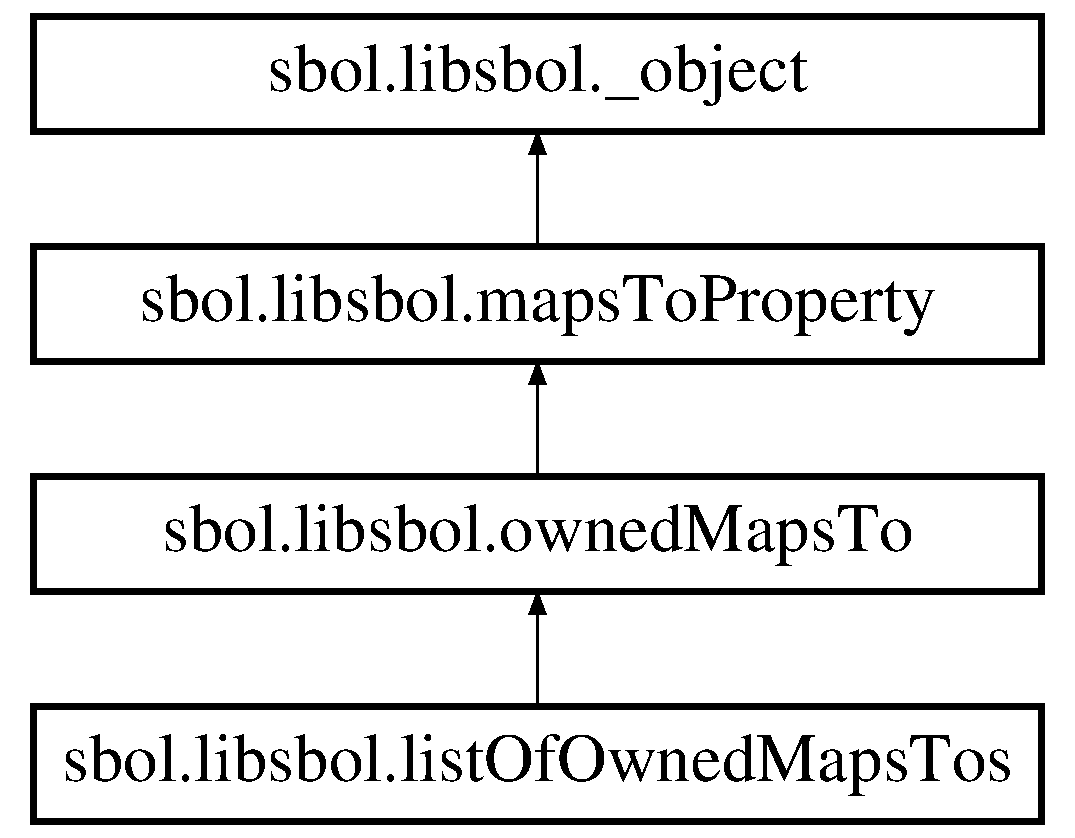
\includegraphics[height=4.000000cm]{classsbol_1_1libsbol_1_1maps_to_property}
\end{center}
\end{figure}
\subsection*{Public Member Functions}
\begin{DoxyCompactItemize}
\item 
def \hyperlink{classsbol_1_1libsbol_1_1maps_to_property_a57016f2b7a412031d2f84dd4d50c79c9}{\+\_\+\+\_\+init\+\_\+\+\_\+} (self, args)
\item 
def \hyperlink{classsbol_1_1libsbol_1_1maps_to_property_ac31548eb48ed3190b0e19fb195272ca5}{get\+Type\+U\+RI} (self)
\item 
def \hyperlink{classsbol_1_1libsbol_1_1maps_to_property_a9769751f67e64b5e02904ab6641630b6}{get\+Owner} (self)
\item 
def \hyperlink{classsbol_1_1libsbol_1_1maps_to_property_ac57c550584bdb347f063116d7e882328}{get} (self)
\item 
def \hyperlink{classsbol_1_1libsbol_1_1maps_to_property_ac9e64d3913383fa98b743df1587e70e1}{add} (self, new\+\_\+value)
\item 
def \hyperlink{classsbol_1_1libsbol_1_1maps_to_property_ab872cc8eb2739aae0391a7763314a269}{set} (self, args)
\item 
def \hyperlink{classsbol_1_1libsbol_1_1maps_to_property_a10d94a5a896a8a65435ea8b0707ace0c}{write} (self)
\item 
def \hyperlink{classsbol_1_1libsbol_1_1maps_to_property_a739540995b53307e76920dbd81da2b73}{validate} (self, arg=None)
\item 
def {\bfseries \+\_\+\+\_\+getitem\+\_\+\+\_\+} (self, n\+Index)\hypertarget{classsbol_1_1libsbol_1_1maps_to_property_a41f770837e8dc9266fc425713b05e497}{}\label{classsbol_1_1libsbol_1_1maps_to_property_a41f770837e8dc9266fc425713b05e497}

\item 
def {\bfseries \+\_\+\+\_\+iter\+\_\+\+\_\+} (self)\hypertarget{classsbol_1_1libsbol_1_1maps_to_property_ae8fffe8f8cb954344fcbb5cae6b33b0b}{}\label{classsbol_1_1libsbol_1_1maps_to_property_ae8fffe8f8cb954344fcbb5cae6b33b0b}

\item 
def {\bfseries next} (self)\hypertarget{classsbol_1_1libsbol_1_1maps_to_property_a7816257a4f095eebbd52453207efdb5c}{}\label{classsbol_1_1libsbol_1_1maps_to_property_a7816257a4f095eebbd52453207efdb5c}

\item 
def {\bfseries \+\_\+\+\_\+len\+\_\+\+\_\+} (self)\hypertarget{classsbol_1_1libsbol_1_1maps_to_property_a19515969e8c77c0dca8e7473d0785431}{}\label{classsbol_1_1libsbol_1_1maps_to_property_a19515969e8c77c0dca8e7473d0785431}

\end{DoxyCompactItemize}
\subsection*{Public Attributes}
\begin{DoxyCompactItemize}
\item 
{\bfseries this}\hypertarget{classsbol_1_1libsbol_1_1maps_to_property_a289b238fcfbdc0c23e6363d0c7058fea}{}\label{classsbol_1_1libsbol_1_1maps_to_property_a289b238fcfbdc0c23e6363d0c7058fea}

\end{DoxyCompactItemize}


\subsection{Detailed Description}
\begin{DoxyVerb}metafunction for generation of a map of message types to their
associated callbacks.

Usage: Use generate_callback_map<Type>::type to ...

Parameters:
-----------

LiteralType:  The library currently supports Property<string> and
Property<int> specification currently supports integer, string, and
URI literals

C++ includes: property.h 
\end{DoxyVerb}
 

\subsection{Constructor \& Destructor Documentation}
\index{sbol\+::libsbol\+::maps\+To\+Property@{sbol\+::libsbol\+::maps\+To\+Property}!\+\_\+\+\_\+init\+\_\+\+\_\+@{\+\_\+\+\_\+init\+\_\+\+\_\+}}
\index{\+\_\+\+\_\+init\+\_\+\+\_\+@{\+\_\+\+\_\+init\+\_\+\+\_\+}!sbol\+::libsbol\+::maps\+To\+Property@{sbol\+::libsbol\+::maps\+To\+Property}}
\subsubsection[{\texorpdfstring{\+\_\+\+\_\+init\+\_\+\+\_\+(self, args)}{__init__(self, args)}}]{\setlength{\rightskip}{0pt plus 5cm}def sbol.\+libsbol.\+maps\+To\+Property.\+\_\+\+\_\+init\+\_\+\+\_\+ (
\begin{DoxyParamCaption}
\item[{}]{self, }
\item[{}]{args}
\end{DoxyParamCaption}
)}\hypertarget{classsbol_1_1libsbol_1_1maps_to_property_a57016f2b7a412031d2f84dd4d50c79c9}{}\label{classsbol_1_1libsbol_1_1maps_to_property_a57016f2b7a412031d2f84dd4d50c79c9}
\begin{DoxyVerb}sbol::Property<
LiteralType >::Property(sbol_type type_uri=UNDEFINED, void
*property_owner=NULL, ValidationRules validation_rules={}) 
\end{DoxyVerb}
 

\subsection{Member Function Documentation}
\index{sbol\+::libsbol\+::maps\+To\+Property@{sbol\+::libsbol\+::maps\+To\+Property}!add@{add}}
\index{add@{add}!sbol\+::libsbol\+::maps\+To\+Property@{sbol\+::libsbol\+::maps\+To\+Property}}
\subsubsection[{\texorpdfstring{add(self, new\+\_\+value)}{add(self, new_value)}}]{\setlength{\rightskip}{0pt plus 5cm}def sbol.\+libsbol.\+maps\+To\+Property.\+add (
\begin{DoxyParamCaption}
\item[{}]{self, }
\item[{}]{new\+\_\+value}
\end{DoxyParamCaption}
)}\hypertarget{classsbol_1_1libsbol_1_1maps_to_property_ac9e64d3913383fa98b743df1587e70e1}{}\label{classsbol_1_1libsbol_1_1maps_to_property_ac9e64d3913383fa98b743df1587e70e1}
\begin{DoxyVerb}void sbol::Property<
LiteralType >::add(std::string new_value) 
\end{DoxyVerb}
 \index{sbol\+::libsbol\+::maps\+To\+Property@{sbol\+::libsbol\+::maps\+To\+Property}!get@{get}}
\index{get@{get}!sbol\+::libsbol\+::maps\+To\+Property@{sbol\+::libsbol\+::maps\+To\+Property}}
\subsubsection[{\texorpdfstring{get(self)}{get(self)}}]{\setlength{\rightskip}{0pt plus 5cm}def sbol.\+libsbol.\+maps\+To\+Property.\+get (
\begin{DoxyParamCaption}
\item[{}]{self}
\end{DoxyParamCaption}
)}\hypertarget{classsbol_1_1libsbol_1_1maps_to_property_ac57c550584bdb347f063116d7e882328}{}\label{classsbol_1_1libsbol_1_1maps_to_property_ac57c550584bdb347f063116d7e882328}
\begin{DoxyVerb}std::string
sbol::Property< LiteralType >::get() 
\end{DoxyVerb}
 \index{sbol\+::libsbol\+::maps\+To\+Property@{sbol\+::libsbol\+::maps\+To\+Property}!get\+Owner@{get\+Owner}}
\index{get\+Owner@{get\+Owner}!sbol\+::libsbol\+::maps\+To\+Property@{sbol\+::libsbol\+::maps\+To\+Property}}
\subsubsection[{\texorpdfstring{get\+Owner(self)}{getOwner(self)}}]{\setlength{\rightskip}{0pt plus 5cm}def sbol.\+libsbol.\+maps\+To\+Property.\+get\+Owner (
\begin{DoxyParamCaption}
\item[{}]{self}
\end{DoxyParamCaption}
)}\hypertarget{classsbol_1_1libsbol_1_1maps_to_property_a9769751f67e64b5e02904ab6641630b6}{}\label{classsbol_1_1libsbol_1_1maps_to_property_a9769751f67e64b5e02904ab6641630b6}
\begin{DoxyVerb}SBOLObject &
sbol::Property< LiteralType >::getOwner() 
\end{DoxyVerb}
 \index{sbol\+::libsbol\+::maps\+To\+Property@{sbol\+::libsbol\+::maps\+To\+Property}!get\+Type\+U\+RI@{get\+Type\+U\+RI}}
\index{get\+Type\+U\+RI@{get\+Type\+U\+RI}!sbol\+::libsbol\+::maps\+To\+Property@{sbol\+::libsbol\+::maps\+To\+Property}}
\subsubsection[{\texorpdfstring{get\+Type\+U\+R\+I(self)}{getTypeURI(self)}}]{\setlength{\rightskip}{0pt plus 5cm}def sbol.\+libsbol.\+maps\+To\+Property.\+get\+Type\+U\+RI (
\begin{DoxyParamCaption}
\item[{}]{self}
\end{DoxyParamCaption}
)}\hypertarget{classsbol_1_1libsbol_1_1maps_to_property_ac31548eb48ed3190b0e19fb195272ca5}{}\label{classsbol_1_1libsbol_1_1maps_to_property_ac31548eb48ed3190b0e19fb195272ca5}
\begin{DoxyVerb}sbol_type
sbol::Property< LiteralType >::getTypeURI() 
\end{DoxyVerb}
 \index{sbol\+::libsbol\+::maps\+To\+Property@{sbol\+::libsbol\+::maps\+To\+Property}!set@{set}}
\index{set@{set}!sbol\+::libsbol\+::maps\+To\+Property@{sbol\+::libsbol\+::maps\+To\+Property}}
\subsubsection[{\texorpdfstring{set(self, args)}{set(self, args)}}]{\setlength{\rightskip}{0pt plus 5cm}def sbol.\+libsbol.\+maps\+To\+Property.\+set (
\begin{DoxyParamCaption}
\item[{}]{self, }
\item[{}]{args}
\end{DoxyParamCaption}
)}\hypertarget{classsbol_1_1libsbol_1_1maps_to_property_ab872cc8eb2739aae0391a7763314a269}{}\label{classsbol_1_1libsbol_1_1maps_to_property_ab872cc8eb2739aae0391a7763314a269}
\begin{DoxyVerb}void sbol::Property<
LiteralType >::set(int new_value) 
\end{DoxyVerb}
 \index{sbol\+::libsbol\+::maps\+To\+Property@{sbol\+::libsbol\+::maps\+To\+Property}!validate@{validate}}
\index{validate@{validate}!sbol\+::libsbol\+::maps\+To\+Property@{sbol\+::libsbol\+::maps\+To\+Property}}
\subsubsection[{\texorpdfstring{validate(self, arg=\+None)}{validate(self, arg=None)}}]{\setlength{\rightskip}{0pt plus 5cm}def sbol.\+libsbol.\+maps\+To\+Property.\+validate (
\begin{DoxyParamCaption}
\item[{}]{self, }
\item[{}]{arg = {\ttfamily None}}
\end{DoxyParamCaption}
)}\hypertarget{classsbol_1_1libsbol_1_1maps_to_property_a739540995b53307e76920dbd81da2b73}{}\label{classsbol_1_1libsbol_1_1maps_to_property_a739540995b53307e76920dbd81da2b73}
\begin{DoxyVerb}void sbol::Property<
LiteralType >::validate(void *arg=NULL) 
\end{DoxyVerb}
 \index{sbol\+::libsbol\+::maps\+To\+Property@{sbol\+::libsbol\+::maps\+To\+Property}!write@{write}}
\index{write@{write}!sbol\+::libsbol\+::maps\+To\+Property@{sbol\+::libsbol\+::maps\+To\+Property}}
\subsubsection[{\texorpdfstring{write(self)}{write(self)}}]{\setlength{\rightskip}{0pt plus 5cm}def sbol.\+libsbol.\+maps\+To\+Property.\+write (
\begin{DoxyParamCaption}
\item[{}]{self}
\end{DoxyParamCaption}
)}\hypertarget{classsbol_1_1libsbol_1_1maps_to_property_a10d94a5a896a8a65435ea8b0707ace0c}{}\label{classsbol_1_1libsbol_1_1maps_to_property_a10d94a5a896a8a65435ea8b0707ace0c}
\begin{DoxyVerb}void sbol::Property<
LiteralType >::write() 
\end{DoxyVerb}
 

The documentation for this class was generated from the following file\+:\begin{DoxyCompactItemize}
\item 
libsbol.\+py\end{DoxyCompactItemize}

\hypertarget{classsbol_1_1libsbol_1_1_model}{}\section{sbol.\+libsbol.\+Model Class Reference}
\label{classsbol_1_1libsbol_1_1_model}\index{sbol.\+libsbol.\+Model@{sbol.\+libsbol.\+Model}}
Inheritance diagram for sbol.\+libsbol.\+Model\+:\begin{figure}[H]
\begin{center}
\leavevmode
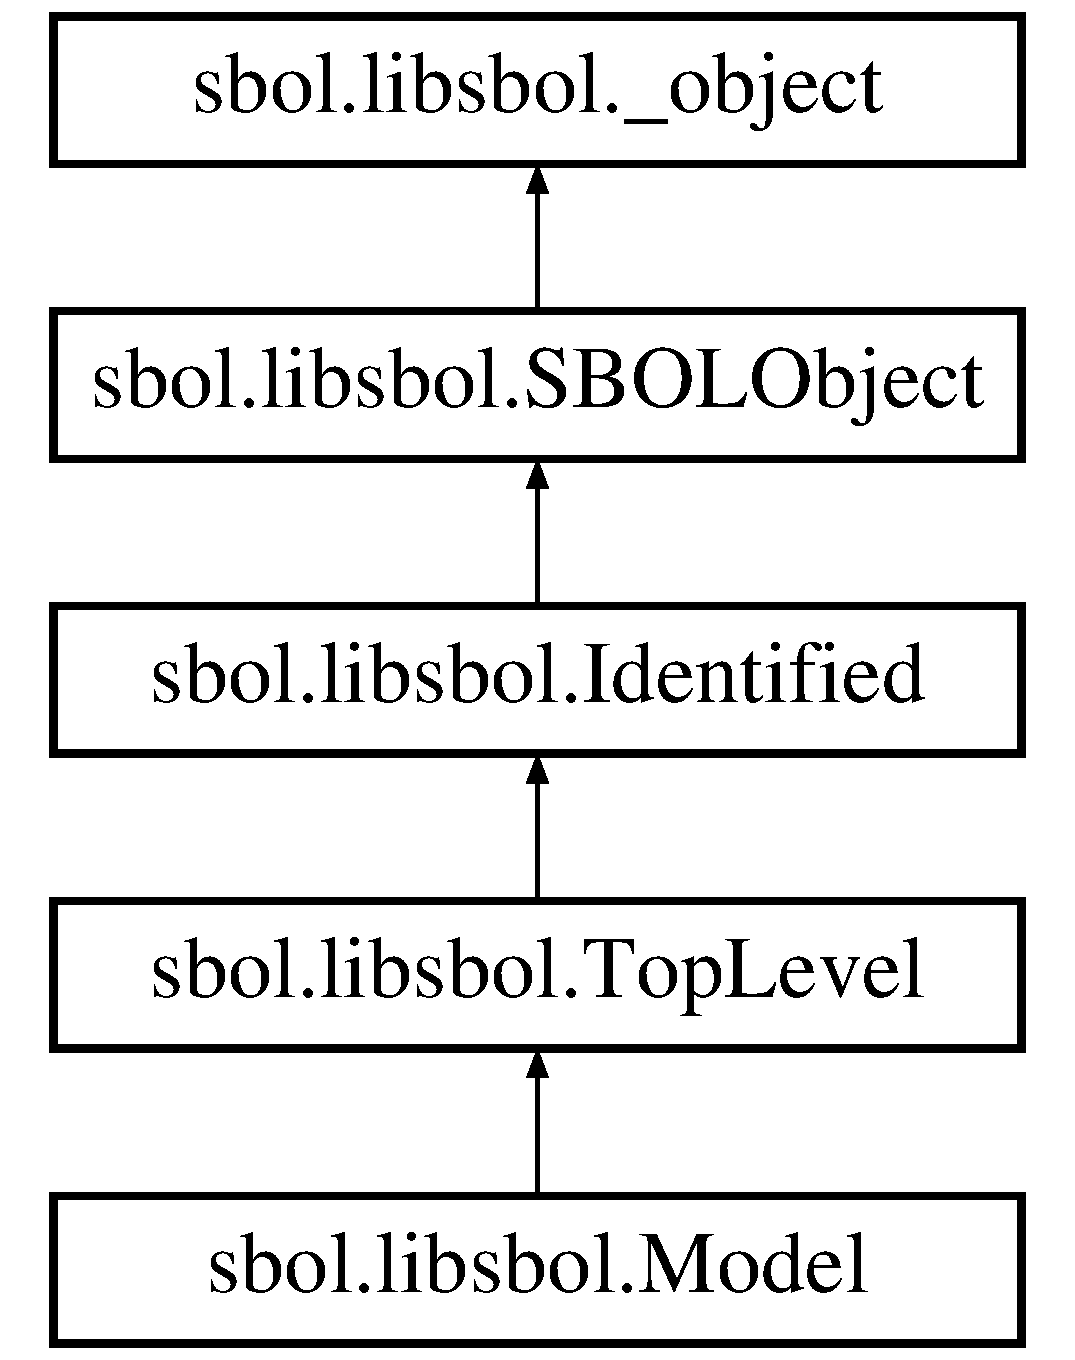
\includegraphics[height=5.000000cm]{classsbol_1_1libsbol_1_1_model}
\end{center}
\end{figure}
\subsection*{Public Member Functions}
\begin{DoxyCompactItemize}
\item 
def \hyperlink{classsbol_1_1libsbol_1_1_model_a246cc573e9da6b1b2b2576885511fff7}{\+\_\+\+\_\+init\+\_\+\+\_\+} (self, args)
\end{DoxyCompactItemize}
\subsection*{Public Attributes}
\begin{DoxyCompactItemize}
\item 
{\bfseries this}\hypertarget{classsbol_1_1libsbol_1_1_model_adbc41a7ed052768e8bf574e6f10fdb1a}{}\label{classsbol_1_1libsbol_1_1_model_adbc41a7ed052768e8bf574e6f10fdb1a}

\end{DoxyCompactItemize}
\subsection*{Static Public Attributes}
\begin{DoxyCompactItemize}
\item 
{\bfseries source} = \+\_\+swig\+\_\+property(\+\_\+libsbol.\+Model\+\_\+source\+\_\+get, \+\_\+libsbol.\+Model\+\_\+source\+\_\+set)\hypertarget{classsbol_1_1libsbol_1_1_model_ae500c02c731f44e19470b99562583860}{}\label{classsbol_1_1libsbol_1_1_model_ae500c02c731f44e19470b99562583860}

\item 
{\bfseries language} = \+\_\+swig\+\_\+property(\+\_\+libsbol.\+Model\+\_\+language\+\_\+get, \+\_\+libsbol.\+Model\+\_\+language\+\_\+set)\hypertarget{classsbol_1_1libsbol_1_1_model_a527f2988adcde814e31f06f5f4600a0a}{}\label{classsbol_1_1libsbol_1_1_model_a527f2988adcde814e31f06f5f4600a0a}

\item 
{\bfseries framework} = \+\_\+swig\+\_\+property(\+\_\+libsbol.\+Model\+\_\+framework\+\_\+get, \+\_\+libsbol.\+Model\+\_\+framework\+\_\+set)\hypertarget{classsbol_1_1libsbol_1_1_model_ac104c9f8c99e5cde26cefb432cf8bad7}{}\label{classsbol_1_1libsbol_1_1_model_ac104c9f8c99e5cde26cefb432cf8bad7}

\end{DoxyCompactItemize}


\subsection{Constructor \& Destructor Documentation}
\index{sbol\+::libsbol\+::\+Model@{sbol\+::libsbol\+::\+Model}!\+\_\+\+\_\+init\+\_\+\+\_\+@{\+\_\+\+\_\+init\+\_\+\+\_\+}}
\index{\+\_\+\+\_\+init\+\_\+\+\_\+@{\+\_\+\+\_\+init\+\_\+\+\_\+}!sbol\+::libsbol\+::\+Model@{sbol\+::libsbol\+::\+Model}}
\subsubsection[{\texorpdfstring{\+\_\+\+\_\+init\+\_\+\+\_\+(self, args)}{__init__(self, args)}}]{\setlength{\rightskip}{0pt plus 5cm}def sbol.\+libsbol.\+Model.\+\_\+\+\_\+init\+\_\+\+\_\+ (
\begin{DoxyParamCaption}
\item[{}]{self, }
\item[{}]{args}
\end{DoxyParamCaption}
)}\hypertarget{classsbol_1_1libsbol_1_1_model_a246cc573e9da6b1b2b2576885511fff7}{}\label{classsbol_1_1libsbol_1_1_model_a246cc573e9da6b1b2b2576885511fff7}
\begin{DoxyVerb}sbol::Model::Model(std::string uri_prefix, std::string display_id,
std::string version, std::string source, std::string language,
std::string framework) 
\end{DoxyVerb}
 

The documentation for this class was generated from the following file\+:\begin{DoxyCompactItemize}
\item 
libsbol.\+py\end{DoxyCompactItemize}

\hypertarget{classsbol_1_1libsbol_1_1_module}{}\section{sbol.\+libsbol.\+Module Class Reference}
\label{classsbol_1_1libsbol_1_1_module}\index{sbol.\+libsbol.\+Module@{sbol.\+libsbol.\+Module}}
Inheritance diagram for sbol.\+libsbol.\+Module\+:\begin{figure}[H]
\begin{center}
\leavevmode
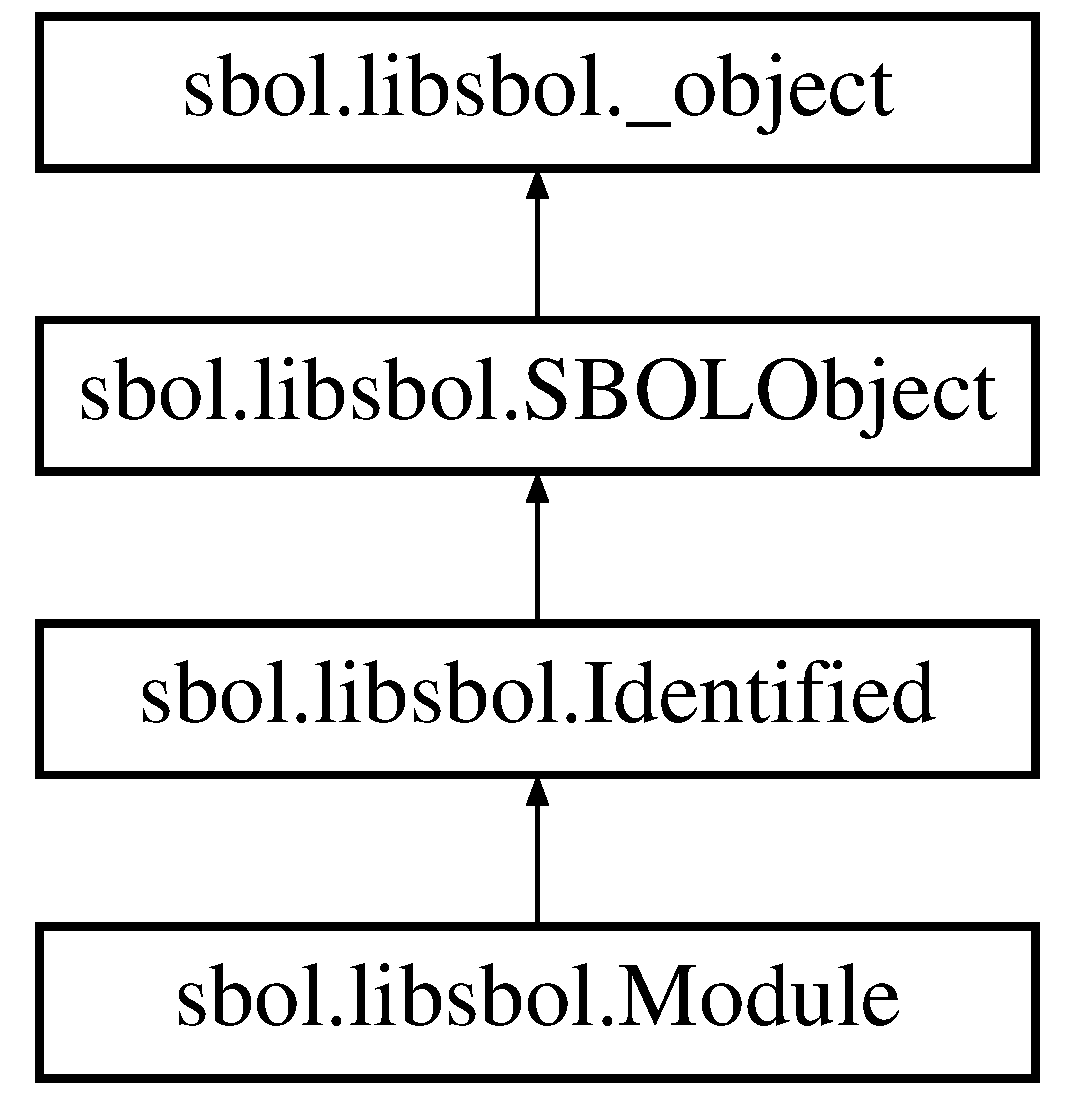
\includegraphics[height=4.000000cm]{classsbol_1_1libsbol_1_1_module}
\end{center}
\end{figure}
\subsection*{Public Member Functions}
\begin{DoxyCompactItemize}
\item 
def \hyperlink{classsbol_1_1libsbol_1_1_module_ac825ddb96ad640999b3171f4d93a3712}{\+\_\+\+\_\+init\+\_\+\+\_\+} (self, args)
\end{DoxyCompactItemize}
\subsection*{Public Attributes}
\begin{DoxyCompactItemize}
\item 
{\bfseries this}\hypertarget{classsbol_1_1libsbol_1_1_module_a914a35bbc2bb00f441892ef5eeab5a0f}{}\label{classsbol_1_1libsbol_1_1_module_a914a35bbc2bb00f441892ef5eeab5a0f}

\end{DoxyCompactItemize}
\subsection*{Static Public Attributes}
\begin{DoxyCompactItemize}
\item 
{\bfseries definition} = \+\_\+swig\+\_\+property(\+\_\+libsbol.\+Module\+\_\+definition\+\_\+get, \+\_\+libsbol.\+Module\+\_\+definition\+\_\+set)\hypertarget{classsbol_1_1libsbol_1_1_module_a98e92fdf926f872c91f69b7f92bbe11e}{}\label{classsbol_1_1libsbol_1_1_module_a98e92fdf926f872c91f69b7f92bbe11e}

\item 
{\bfseries maps\+Tos} = \+\_\+swig\+\_\+property(\+\_\+libsbol.\+Module\+\_\+maps\+Tos\+\_\+get, \+\_\+libsbol.\+Module\+\_\+maps\+Tos\+\_\+set)\hypertarget{classsbol_1_1libsbol_1_1_module_a7710fec04decd56eda791d067145ba5c}{}\label{classsbol_1_1libsbol_1_1_module_a7710fec04decd56eda791d067145ba5c}

\end{DoxyCompactItemize}


\subsection{Constructor \& Destructor Documentation}
\index{sbol\+::libsbol\+::\+Module@{sbol\+::libsbol\+::\+Module}!\+\_\+\+\_\+init\+\_\+\+\_\+@{\+\_\+\+\_\+init\+\_\+\+\_\+}}
\index{\+\_\+\+\_\+init\+\_\+\+\_\+@{\+\_\+\+\_\+init\+\_\+\+\_\+}!sbol\+::libsbol\+::\+Module@{sbol\+::libsbol\+::\+Module}}
\subsubsection[{\texorpdfstring{\+\_\+\+\_\+init\+\_\+\+\_\+(self, args)}{__init__(self, args)}}]{\setlength{\rightskip}{0pt plus 5cm}def sbol.\+libsbol.\+Module.\+\_\+\+\_\+init\+\_\+\+\_\+ (
\begin{DoxyParamCaption}
\item[{}]{self, }
\item[{}]{args}
\end{DoxyParamCaption}
)}\hypertarget{classsbol_1_1libsbol_1_1_module_ac825ddb96ad640999b3171f4d93a3712}{}\label{classsbol_1_1libsbol_1_1_module_ac825ddb96ad640999b3171f4d93a3712}
\begin{DoxyVerb}sbol::Module::Module(std::string uri_prefix, std::string display_id,
std::string version, std::string definition) 
\end{DoxyVerb}
 

The documentation for this class was generated from the following file\+:\begin{DoxyCompactItemize}
\item 
libsbol.\+py\end{DoxyCompactItemize}

\hypertarget{classsbol_1_1libsbol_1_1_module_definition}{}\section{sbol.\+libsbol.\+Module\+Definition Class Reference}
\label{classsbol_1_1libsbol_1_1_module_definition}\index{sbol.\+libsbol.\+Module\+Definition@{sbol.\+libsbol.\+Module\+Definition}}
Inheritance diagram for sbol.\+libsbol.\+Module\+Definition\+:\begin{figure}[H]
\begin{center}
\leavevmode
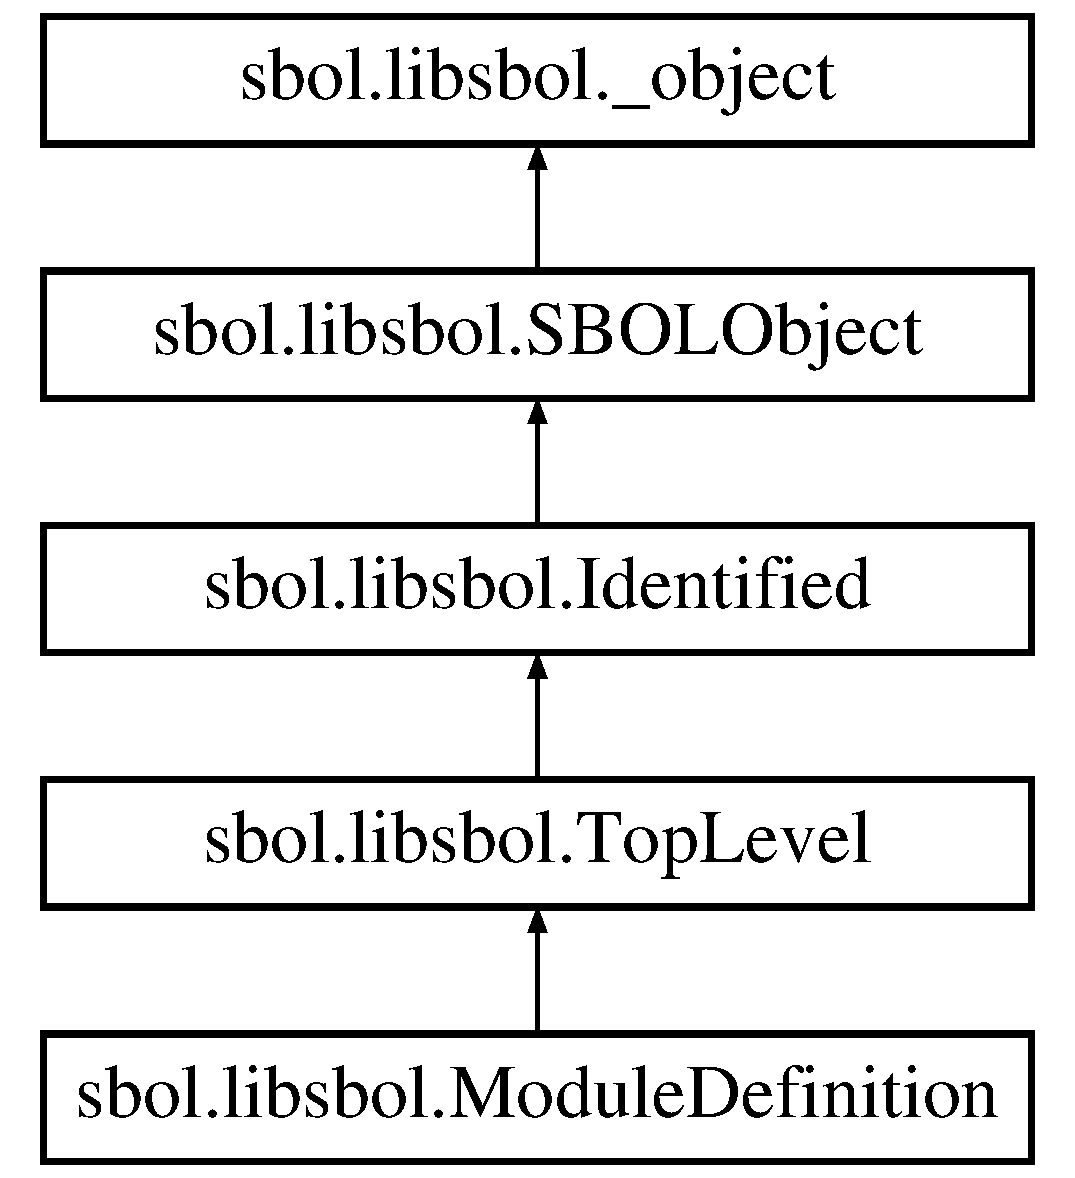
\includegraphics[height=5.000000cm]{classsbol_1_1libsbol_1_1_module_definition}
\end{center}
\end{figure}
\subsection*{Public Member Functions}
\begin{DoxyCompactItemize}
\item 
def \hyperlink{classsbol_1_1libsbol_1_1_module_definition_a05b80625efcb0b70221a696ce800e1ba}{\+\_\+\+\_\+init\+\_\+\+\_\+} (self, args)
\end{DoxyCompactItemize}
\subsection*{Public Attributes}
\begin{DoxyCompactItemize}
\item 
{\bfseries this}\hypertarget{classsbol_1_1libsbol_1_1_module_definition_aef145d12a34c7618e9bbfe7b9d568017}{}\label{classsbol_1_1libsbol_1_1_module_definition_aef145d12a34c7618e9bbfe7b9d568017}

\end{DoxyCompactItemize}
\subsection*{Static Public Attributes}
\begin{DoxyCompactItemize}
\item 
{\bfseries roles} = \+\_\+swig\+\_\+property(\+\_\+libsbol.\+Module\+Definition\+\_\+roles\+\_\+get, \+\_\+libsbol.\+Module\+Definition\+\_\+roles\+\_\+set)\hypertarget{classsbol_1_1libsbol_1_1_module_definition_ad148da94e2f436f3c1ffea6e014b5e69}{}\label{classsbol_1_1libsbol_1_1_module_definition_ad148da94e2f436f3c1ffea6e014b5e69}

\item 
{\bfseries modules} = \+\_\+swig\+\_\+property(\+\_\+libsbol.\+Module\+Definition\+\_\+modules\+\_\+get, \+\_\+libsbol.\+Module\+Definition\+\_\+modules\+\_\+set)\hypertarget{classsbol_1_1libsbol_1_1_module_definition_a73661dd5c57ed87e5a71d8b11dabc9a3}{}\label{classsbol_1_1libsbol_1_1_module_definition_a73661dd5c57ed87e5a71d8b11dabc9a3}

\item 
{\bfseries interactions} = \+\_\+swig\+\_\+property(\+\_\+libsbol.\+Module\+Definition\+\_\+interactions\+\_\+get, \+\_\+libsbol.\+Module\+Definition\+\_\+interactions\+\_\+set)\hypertarget{classsbol_1_1libsbol_1_1_module_definition_a83c6cdf559f6ecf2423ed5c0d71c427a}{}\label{classsbol_1_1libsbol_1_1_module_definition_a83c6cdf559f6ecf2423ed5c0d71c427a}

\item 
{\bfseries functional\+Components} = \+\_\+swig\+\_\+property(\+\_\+libsbol.\+Module\+Definition\+\_\+functional\+Components\+\_\+get, \+\_\+libsbol.\+Module\+Definition\+\_\+functional\+Components\+\_\+set)\hypertarget{classsbol_1_1libsbol_1_1_module_definition_a497d48f12548a91ce2012a2b0c27fea8}{}\label{classsbol_1_1libsbol_1_1_module_definition_a497d48f12548a91ce2012a2b0c27fea8}

\item 
{\bfseries models} = \+\_\+swig\+\_\+property(\+\_\+libsbol.\+Module\+Definition\+\_\+models\+\_\+get, \+\_\+libsbol.\+Module\+Definition\+\_\+models\+\_\+set)\hypertarget{classsbol_1_1libsbol_1_1_module_definition_a9798d2e776acbecc3a5a4bed51695b80}{}\label{classsbol_1_1libsbol_1_1_module_definition_a9798d2e776acbecc3a5a4bed51695b80}

\end{DoxyCompactItemize}


\subsection{Constructor \& Destructor Documentation}
\index{sbol\+::libsbol\+::\+Module\+Definition@{sbol\+::libsbol\+::\+Module\+Definition}!\+\_\+\+\_\+init\+\_\+\+\_\+@{\+\_\+\+\_\+init\+\_\+\+\_\+}}
\index{\+\_\+\+\_\+init\+\_\+\+\_\+@{\+\_\+\+\_\+init\+\_\+\+\_\+}!sbol\+::libsbol\+::\+Module\+Definition@{sbol\+::libsbol\+::\+Module\+Definition}}
\subsubsection[{\texorpdfstring{\+\_\+\+\_\+init\+\_\+\+\_\+(self, args)}{__init__(self, args)}}]{\setlength{\rightskip}{0pt plus 5cm}def sbol.\+libsbol.\+Module\+Definition.\+\_\+\+\_\+init\+\_\+\+\_\+ (
\begin{DoxyParamCaption}
\item[{}]{self, }
\item[{}]{args}
\end{DoxyParamCaption}
)}\hypertarget{classsbol_1_1libsbol_1_1_module_definition_a05b80625efcb0b70221a696ce800e1ba}{}\label{classsbol_1_1libsbol_1_1_module_definition_a05b80625efcb0b70221a696ce800e1ba}
\begin{DoxyVerb}sbol::ModuleDefinition::ModuleDefinition(std::string uri_prefix,
std::string display_id, std::string version) 
\end{DoxyVerb}
 

The documentation for this class was generated from the following file\+:\begin{DoxyCompactItemize}
\item 
libsbol.\+py\end{DoxyCompactItemize}

\hypertarget{classsbol_1_1libsbol_1_1module_property}{}\section{sbol.\+libsbol.\+module\+Property Class Reference}
\label{classsbol_1_1libsbol_1_1module_property}\index{sbol.\+libsbol.\+module\+Property@{sbol.\+libsbol.\+module\+Property}}
Inheritance diagram for sbol.\+libsbol.\+module\+Property\+:\begin{figure}[H]
\begin{center}
\leavevmode
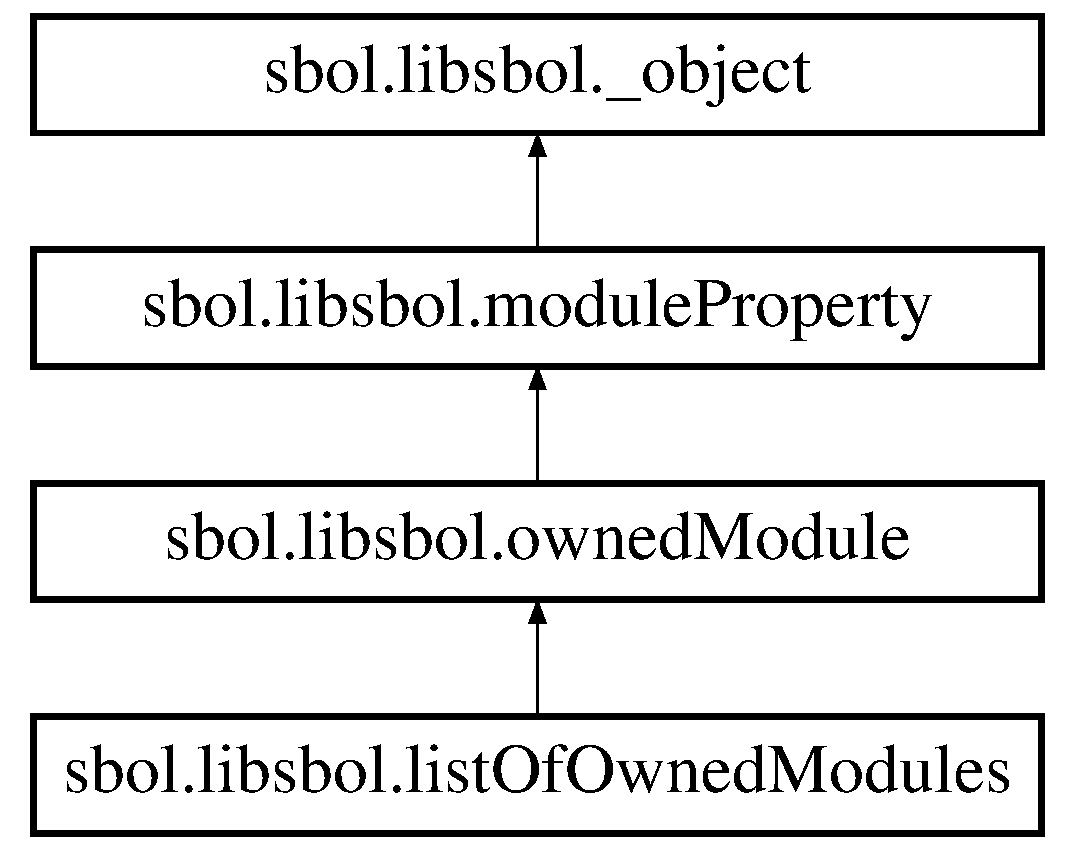
\includegraphics[height=4.000000cm]{classsbol_1_1libsbol_1_1module_property}
\end{center}
\end{figure}
\subsection*{Public Member Functions}
\begin{DoxyCompactItemize}
\item 
def \hyperlink{classsbol_1_1libsbol_1_1module_property_ad6a0f5eb06afa467e76804f34804f850}{\+\_\+\+\_\+init\+\_\+\+\_\+} (self, args)
\item 
def \hyperlink{classsbol_1_1libsbol_1_1module_property_a2efaeb3d0c2ef63a544d14dc19754de8}{get\+Type\+U\+RI} (self)
\item 
def \hyperlink{classsbol_1_1libsbol_1_1module_property_acf8e1981bebada31bed5b2c8869bfc63}{get\+Owner} (self)
\item 
def \hyperlink{classsbol_1_1libsbol_1_1module_property_a9e7d6f666f70655582d10468fb2c163a}{get} (self)
\item 
def \hyperlink{classsbol_1_1libsbol_1_1module_property_a1bedbc87f8d0493a1b2be9dd3f4288ac}{add} (self, new\+\_\+value)
\item 
def \hyperlink{classsbol_1_1libsbol_1_1module_property_a68871e405351fb7480477e54e30095e8}{set} (self, args)
\item 
def \hyperlink{classsbol_1_1libsbol_1_1module_property_aa5509d0bfa5abb817737df78e13f5935}{write} (self)
\item 
def \hyperlink{classsbol_1_1libsbol_1_1module_property_a75641a46d49ea4586ff2f7673dc7a617}{validate} (self, arg=None)
\item 
def {\bfseries \+\_\+\+\_\+getitem\+\_\+\+\_\+} (self, n\+Index)\hypertarget{classsbol_1_1libsbol_1_1module_property_a734fe4482e1fe2d18eec3725b2f38f0a}{}\label{classsbol_1_1libsbol_1_1module_property_a734fe4482e1fe2d18eec3725b2f38f0a}

\item 
def {\bfseries \+\_\+\+\_\+iter\+\_\+\+\_\+} (self)\hypertarget{classsbol_1_1libsbol_1_1module_property_ad2d77e7994947a5beb840214076141fc}{}\label{classsbol_1_1libsbol_1_1module_property_ad2d77e7994947a5beb840214076141fc}

\item 
def {\bfseries next} (self)\hypertarget{classsbol_1_1libsbol_1_1module_property_ade25c1ff8a2ddea54b38a0c453e4243b}{}\label{classsbol_1_1libsbol_1_1module_property_ade25c1ff8a2ddea54b38a0c453e4243b}

\item 
def {\bfseries \+\_\+\+\_\+len\+\_\+\+\_\+} (self)\hypertarget{classsbol_1_1libsbol_1_1module_property_abdbbef9752bcf852f6caf855e1d8dd81}{}\label{classsbol_1_1libsbol_1_1module_property_abdbbef9752bcf852f6caf855e1d8dd81}

\end{DoxyCompactItemize}
\subsection*{Public Attributes}
\begin{DoxyCompactItemize}
\item 
{\bfseries this}\hypertarget{classsbol_1_1libsbol_1_1module_property_a6d4da1916212c7ecd0ecc909786df9d9}{}\label{classsbol_1_1libsbol_1_1module_property_a6d4da1916212c7ecd0ecc909786df9d9}

\end{DoxyCompactItemize}


\subsection{Detailed Description}
\begin{DoxyVerb}metafunction for generation of a map of message types to their
associated callbacks.

Usage: Use generate_callback_map<Type>::type to ...

Parameters:
-----------

LiteralType:  The library currently supports Property<string> and
Property<int> specification currently supports integer, string, and
URI literals

C++ includes: property.h 
\end{DoxyVerb}
 

\subsection{Constructor \& Destructor Documentation}
\index{sbol\+::libsbol\+::module\+Property@{sbol\+::libsbol\+::module\+Property}!\+\_\+\+\_\+init\+\_\+\+\_\+@{\+\_\+\+\_\+init\+\_\+\+\_\+}}
\index{\+\_\+\+\_\+init\+\_\+\+\_\+@{\+\_\+\+\_\+init\+\_\+\+\_\+}!sbol\+::libsbol\+::module\+Property@{sbol\+::libsbol\+::module\+Property}}
\subsubsection[{\texorpdfstring{\+\_\+\+\_\+init\+\_\+\+\_\+(self, args)}{__init__(self, args)}}]{\setlength{\rightskip}{0pt plus 5cm}def sbol.\+libsbol.\+module\+Property.\+\_\+\+\_\+init\+\_\+\+\_\+ (
\begin{DoxyParamCaption}
\item[{}]{self, }
\item[{}]{args}
\end{DoxyParamCaption}
)}\hypertarget{classsbol_1_1libsbol_1_1module_property_ad6a0f5eb06afa467e76804f34804f850}{}\label{classsbol_1_1libsbol_1_1module_property_ad6a0f5eb06afa467e76804f34804f850}
\begin{DoxyVerb}sbol::Property<
LiteralType >::Property(sbol_type type_uri=UNDEFINED, void
*property_owner=NULL, ValidationRules validation_rules={}) 
\end{DoxyVerb}
 

\subsection{Member Function Documentation}
\index{sbol\+::libsbol\+::module\+Property@{sbol\+::libsbol\+::module\+Property}!add@{add}}
\index{add@{add}!sbol\+::libsbol\+::module\+Property@{sbol\+::libsbol\+::module\+Property}}
\subsubsection[{\texorpdfstring{add(self, new\+\_\+value)}{add(self, new_value)}}]{\setlength{\rightskip}{0pt plus 5cm}def sbol.\+libsbol.\+module\+Property.\+add (
\begin{DoxyParamCaption}
\item[{}]{self, }
\item[{}]{new\+\_\+value}
\end{DoxyParamCaption}
)}\hypertarget{classsbol_1_1libsbol_1_1module_property_a1bedbc87f8d0493a1b2be9dd3f4288ac}{}\label{classsbol_1_1libsbol_1_1module_property_a1bedbc87f8d0493a1b2be9dd3f4288ac}
\begin{DoxyVerb}void sbol::Property<
LiteralType >::add(std::string new_value) 
\end{DoxyVerb}
 \index{sbol\+::libsbol\+::module\+Property@{sbol\+::libsbol\+::module\+Property}!get@{get}}
\index{get@{get}!sbol\+::libsbol\+::module\+Property@{sbol\+::libsbol\+::module\+Property}}
\subsubsection[{\texorpdfstring{get(self)}{get(self)}}]{\setlength{\rightskip}{0pt plus 5cm}def sbol.\+libsbol.\+module\+Property.\+get (
\begin{DoxyParamCaption}
\item[{}]{self}
\end{DoxyParamCaption}
)}\hypertarget{classsbol_1_1libsbol_1_1module_property_a9e7d6f666f70655582d10468fb2c163a}{}\label{classsbol_1_1libsbol_1_1module_property_a9e7d6f666f70655582d10468fb2c163a}
\begin{DoxyVerb}std::string
sbol::Property< LiteralType >::get() 
\end{DoxyVerb}
 \index{sbol\+::libsbol\+::module\+Property@{sbol\+::libsbol\+::module\+Property}!get\+Owner@{get\+Owner}}
\index{get\+Owner@{get\+Owner}!sbol\+::libsbol\+::module\+Property@{sbol\+::libsbol\+::module\+Property}}
\subsubsection[{\texorpdfstring{get\+Owner(self)}{getOwner(self)}}]{\setlength{\rightskip}{0pt plus 5cm}def sbol.\+libsbol.\+module\+Property.\+get\+Owner (
\begin{DoxyParamCaption}
\item[{}]{self}
\end{DoxyParamCaption}
)}\hypertarget{classsbol_1_1libsbol_1_1module_property_acf8e1981bebada31bed5b2c8869bfc63}{}\label{classsbol_1_1libsbol_1_1module_property_acf8e1981bebada31bed5b2c8869bfc63}
\begin{DoxyVerb}SBOLObject &
sbol::Property< LiteralType >::getOwner() 
\end{DoxyVerb}
 \index{sbol\+::libsbol\+::module\+Property@{sbol\+::libsbol\+::module\+Property}!get\+Type\+U\+RI@{get\+Type\+U\+RI}}
\index{get\+Type\+U\+RI@{get\+Type\+U\+RI}!sbol\+::libsbol\+::module\+Property@{sbol\+::libsbol\+::module\+Property}}
\subsubsection[{\texorpdfstring{get\+Type\+U\+R\+I(self)}{getTypeURI(self)}}]{\setlength{\rightskip}{0pt plus 5cm}def sbol.\+libsbol.\+module\+Property.\+get\+Type\+U\+RI (
\begin{DoxyParamCaption}
\item[{}]{self}
\end{DoxyParamCaption}
)}\hypertarget{classsbol_1_1libsbol_1_1module_property_a2efaeb3d0c2ef63a544d14dc19754de8}{}\label{classsbol_1_1libsbol_1_1module_property_a2efaeb3d0c2ef63a544d14dc19754de8}
\begin{DoxyVerb}sbol_type
sbol::Property< LiteralType >::getTypeURI() 
\end{DoxyVerb}
 \index{sbol\+::libsbol\+::module\+Property@{sbol\+::libsbol\+::module\+Property}!set@{set}}
\index{set@{set}!sbol\+::libsbol\+::module\+Property@{sbol\+::libsbol\+::module\+Property}}
\subsubsection[{\texorpdfstring{set(self, args)}{set(self, args)}}]{\setlength{\rightskip}{0pt plus 5cm}def sbol.\+libsbol.\+module\+Property.\+set (
\begin{DoxyParamCaption}
\item[{}]{self, }
\item[{}]{args}
\end{DoxyParamCaption}
)}\hypertarget{classsbol_1_1libsbol_1_1module_property_a68871e405351fb7480477e54e30095e8}{}\label{classsbol_1_1libsbol_1_1module_property_a68871e405351fb7480477e54e30095e8}
\begin{DoxyVerb}void sbol::Property<
LiteralType >::set(int new_value) 
\end{DoxyVerb}
 \index{sbol\+::libsbol\+::module\+Property@{sbol\+::libsbol\+::module\+Property}!validate@{validate}}
\index{validate@{validate}!sbol\+::libsbol\+::module\+Property@{sbol\+::libsbol\+::module\+Property}}
\subsubsection[{\texorpdfstring{validate(self, arg=\+None)}{validate(self, arg=None)}}]{\setlength{\rightskip}{0pt plus 5cm}def sbol.\+libsbol.\+module\+Property.\+validate (
\begin{DoxyParamCaption}
\item[{}]{self, }
\item[{}]{arg = {\ttfamily None}}
\end{DoxyParamCaption}
)}\hypertarget{classsbol_1_1libsbol_1_1module_property_a75641a46d49ea4586ff2f7673dc7a617}{}\label{classsbol_1_1libsbol_1_1module_property_a75641a46d49ea4586ff2f7673dc7a617}
\begin{DoxyVerb}void sbol::Property<
LiteralType >::validate(void *arg=NULL) 
\end{DoxyVerb}
 \index{sbol\+::libsbol\+::module\+Property@{sbol\+::libsbol\+::module\+Property}!write@{write}}
\index{write@{write}!sbol\+::libsbol\+::module\+Property@{sbol\+::libsbol\+::module\+Property}}
\subsubsection[{\texorpdfstring{write(self)}{write(self)}}]{\setlength{\rightskip}{0pt plus 5cm}def sbol.\+libsbol.\+module\+Property.\+write (
\begin{DoxyParamCaption}
\item[{}]{self}
\end{DoxyParamCaption}
)}\hypertarget{classsbol_1_1libsbol_1_1module_property_aa5509d0bfa5abb817737df78e13f5935}{}\label{classsbol_1_1libsbol_1_1module_property_aa5509d0bfa5abb817737df78e13f5935}
\begin{DoxyVerb}void sbol::Property<
LiteralType >::write() 
\end{DoxyVerb}
 

The documentation for this class was generated from the following file\+:\begin{DoxyCompactItemize}
\item 
libsbol.\+py\end{DoxyCompactItemize}

\hypertarget{classsbol_1_1libsbol_1_1owned_functional_component}{}\section{sbol.\+libsbol.\+owned\+Functional\+Component Class Reference}
\label{classsbol_1_1libsbol_1_1owned_functional_component}\index{sbol.\+libsbol.\+owned\+Functional\+Component@{sbol.\+libsbol.\+owned\+Functional\+Component}}
Inheritance diagram for sbol.\+libsbol.\+owned\+Functional\+Component\+:\begin{figure}[H]
\begin{center}
\leavevmode
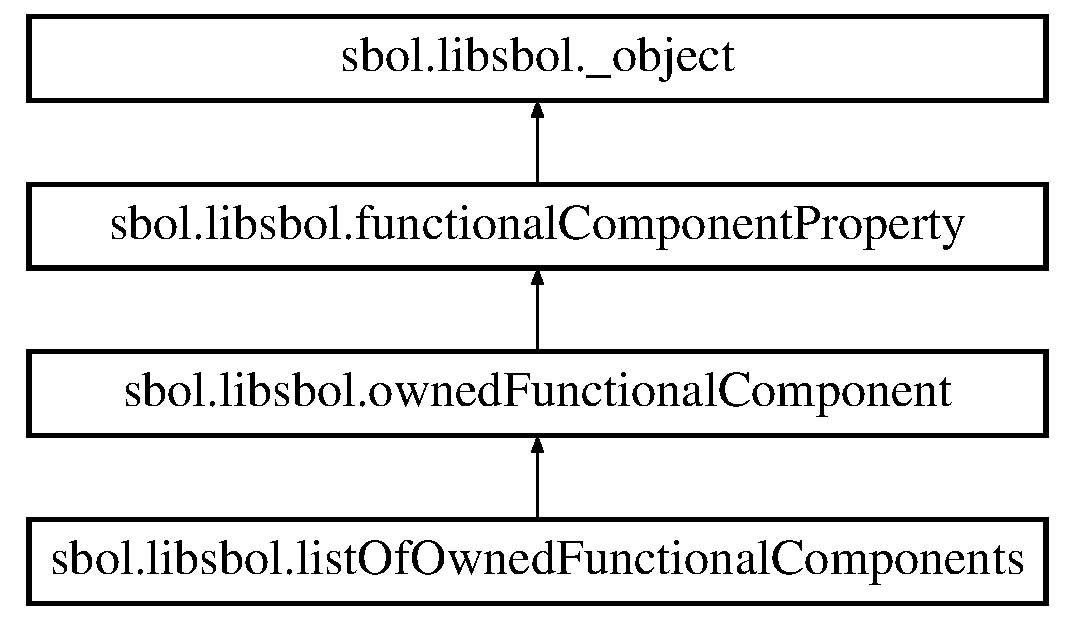
\includegraphics[height=4.000000cm]{classsbol_1_1libsbol_1_1owned_functional_component}
\end{center}
\end{figure}
\subsection*{Public Member Functions}
\begin{DoxyCompactItemize}
\item 
def \hyperlink{classsbol_1_1libsbol_1_1owned_functional_component_a641b5b9d61c83183a2b0c69fd75ffed6}{\+\_\+\+\_\+init\+\_\+\+\_\+} (self, args)
\item 
def \hyperlink{classsbol_1_1libsbol_1_1owned_functional_component_a27eee7b3dcd7f264b67ddd9fc5448add}{add} (self, sbol\+\_\+obj)
\item 
def \hyperlink{classsbol_1_1libsbol_1_1owned_functional_component_a97ed548b2d5b1e3f4e6aff1c495b4aaa}{set} (self, sbol\+\_\+obj)
\item 
def \hyperlink{classsbol_1_1libsbol_1_1owned_functional_component_a22058e0535fe80bd453a9a6e1c449c19}{get} (self, object\+\_\+id)
\item 
def \hyperlink{classsbol_1_1libsbol_1_1owned_functional_component_a33ef3a11b9f63e644d6aabcad930c639}{copy} (self)
\item 
def \hyperlink{classsbol_1_1libsbol_1_1owned_functional_component_a8637492f3e08056ffa5ea7ee027719d8}{create} (self, args)
\item 
def \hyperlink{classsbol_1_1libsbol_1_1owned_functional_component_a77ccc85e71a6452459925a416b28f621}{begin} (self)
\item 
def \hyperlink{classsbol_1_1libsbol_1_1owned_functional_component_a0cd75cae37dd06ac658891896d1c4358}{end} (self)
\item 
def {\bfseries size} (self)\hypertarget{classsbol_1_1libsbol_1_1owned_functional_component_abb82d114d11ed14f80ee45c8abb2816f}{}\label{classsbol_1_1libsbol_1_1owned_functional_component_abb82d114d11ed14f80ee45c8abb2816f}

\item 
def {\bfseries \+\_\+\+\_\+getitem\+\_\+\+\_\+} (self, args)\hypertarget{classsbol_1_1libsbol_1_1owned_functional_component_ae43d6e37dd933155adf4850eff4ba812}{}\label{classsbol_1_1libsbol_1_1owned_functional_component_ae43d6e37dd933155adf4850eff4ba812}

\item 
def {\bfseries \+\_\+\+\_\+iter\+\_\+\+\_\+} (self)\hypertarget{classsbol_1_1libsbol_1_1owned_functional_component_a1cad01362a40e549b892344375ea0182}{}\label{classsbol_1_1libsbol_1_1owned_functional_component_a1cad01362a40e549b892344375ea0182}

\item 
def {\bfseries next} (self)\hypertarget{classsbol_1_1libsbol_1_1owned_functional_component_ac23c5e9b4ae19686a8407624de22d02d}{}\label{classsbol_1_1libsbol_1_1owned_functional_component_ac23c5e9b4ae19686a8407624de22d02d}

\item 
def {\bfseries \+\_\+\+\_\+len\+\_\+\+\_\+} (self)\hypertarget{classsbol_1_1libsbol_1_1owned_functional_component_a75395607bdf31ab50bc5af8710efba52}{}\label{classsbol_1_1libsbol_1_1owned_functional_component_a75395607bdf31ab50bc5af8710efba52}

\item 
def \hyperlink{classsbol_1_1libsbol_1_1owned_functional_component_ac93e6c380b9fd17b91ebca3059dd36b1}{add\+Range} (self, sbol\+\_\+obj)
\item 
def \hyperlink{classsbol_1_1libsbol_1_1owned_functional_component_adfca3d62e9713250213c8ce5db9da51c}{get\+Range} (self)
\end{DoxyCompactItemize}
\subsection*{Public Attributes}
\begin{DoxyCompactItemize}
\item 
{\bfseries this}\hypertarget{classsbol_1_1libsbol_1_1owned_functional_component_a63f58981fe89901406e4c4e8e426fb72}{}\label{classsbol_1_1libsbol_1_1owned_functional_component_a63f58981fe89901406e4c4e8e426fb72}

\end{DoxyCompactItemize}
\subsection*{Static Public Attributes}
\begin{DoxyCompactItemize}
\item 
{\bfseries python\+\_\+iter} = \+\_\+swig\+\_\+property(\+\_\+libsbol.\+owned\+Functional\+Component\+\_\+python\+\_\+iter\+\_\+get, \+\_\+libsbol.\+owned\+Functional\+Component\+\_\+python\+\_\+iter\+\_\+set)\hypertarget{classsbol_1_1libsbol_1_1owned_functional_component_a3c48e8b39cd59dfca924c2549dd80656}{}\label{classsbol_1_1libsbol_1_1owned_functional_component_a3c48e8b39cd59dfca924c2549dd80656}

\end{DoxyCompactItemize}


\subsection{Constructor \& Destructor Documentation}
\index{sbol\+::libsbol\+::owned\+Functional\+Component@{sbol\+::libsbol\+::owned\+Functional\+Component}!\+\_\+\+\_\+init\+\_\+\+\_\+@{\+\_\+\+\_\+init\+\_\+\+\_\+}}
\index{\+\_\+\+\_\+init\+\_\+\+\_\+@{\+\_\+\+\_\+init\+\_\+\+\_\+}!sbol\+::libsbol\+::owned\+Functional\+Component@{sbol\+::libsbol\+::owned\+Functional\+Component}}
\subsubsection[{\texorpdfstring{\+\_\+\+\_\+init\+\_\+\+\_\+(self, args)}{__init__(self, args)}}]{\setlength{\rightskip}{0pt plus 5cm}def sbol.\+libsbol.\+owned\+Functional\+Component.\+\_\+\+\_\+init\+\_\+\+\_\+ (
\begin{DoxyParamCaption}
\item[{}]{self, }
\item[{}]{args}
\end{DoxyParamCaption}
)}\hypertarget{classsbol_1_1libsbol_1_1owned_functional_component_a641b5b9d61c83183a2b0c69fd75ffed6}{}\label{classsbol_1_1libsbol_1_1owned_functional_component_a641b5b9d61c83183a2b0c69fd75ffed6}
\begin{DoxyVerb}sbol::OwnedObject< SBOLClass >::OwnedObject(sbol_type type_uri, void
*property_owner, SBOLObject &first_object) 
\end{DoxyVerb}
 

\subsection{Member Function Documentation}
\index{sbol\+::libsbol\+::owned\+Functional\+Component@{sbol\+::libsbol\+::owned\+Functional\+Component}!add@{add}}
\index{add@{add}!sbol\+::libsbol\+::owned\+Functional\+Component@{sbol\+::libsbol\+::owned\+Functional\+Component}}
\subsubsection[{\texorpdfstring{add(self, sbol\+\_\+obj)}{add(self, sbol_obj)}}]{\setlength{\rightskip}{0pt plus 5cm}def sbol.\+libsbol.\+owned\+Functional\+Component.\+add (
\begin{DoxyParamCaption}
\item[{}]{self, }
\item[{}]{sbol\+\_\+obj}
\end{DoxyParamCaption}
)}\hypertarget{classsbol_1_1libsbol_1_1owned_functional_component_a27eee7b3dcd7f264b67ddd9fc5448add}{}\label{classsbol_1_1libsbol_1_1owned_functional_component_a27eee7b3dcd7f264b67ddd9fc5448add}
\begin{DoxyVerb}void
sbol::OwnedObject< SBOLClass >::add(SBOLClass &sbol_obj) 
\end{DoxyVerb}
 \index{sbol\+::libsbol\+::owned\+Functional\+Component@{sbol\+::libsbol\+::owned\+Functional\+Component}!add\+Range@{add\+Range}}
\index{add\+Range@{add\+Range}!sbol\+::libsbol\+::owned\+Functional\+Component@{sbol\+::libsbol\+::owned\+Functional\+Component}}
\subsubsection[{\texorpdfstring{add\+Range(self, sbol\+\_\+obj)}{addRange(self, sbol_obj)}}]{\setlength{\rightskip}{0pt plus 5cm}def sbol.\+libsbol.\+owned\+Functional\+Component.\+add\+Range (
\begin{DoxyParamCaption}
\item[{}]{self, }
\item[{}]{sbol\+\_\+obj}
\end{DoxyParamCaption}
)}\hypertarget{classsbol_1_1libsbol_1_1owned_functional_component_ac93e6c380b9fd17b91ebca3059dd36b1}{}\label{classsbol_1_1libsbol_1_1owned_functional_component_ac93e6c380b9fd17b91ebca3059dd36b1}
\begin{DoxyVerb}void
sbol::OwnedObject< SBOLClass >::add(SBOLClass &sbol_obj) 
\end{DoxyVerb}
 \index{sbol\+::libsbol\+::owned\+Functional\+Component@{sbol\+::libsbol\+::owned\+Functional\+Component}!begin@{begin}}
\index{begin@{begin}!sbol\+::libsbol\+::owned\+Functional\+Component@{sbol\+::libsbol\+::owned\+Functional\+Component}}
\subsubsection[{\texorpdfstring{begin(self)}{begin(self)}}]{\setlength{\rightskip}{0pt plus 5cm}def sbol.\+libsbol.\+owned\+Functional\+Component.\+begin (
\begin{DoxyParamCaption}
\item[{}]{self}
\end{DoxyParamCaption}
)}\hypertarget{classsbol_1_1libsbol_1_1owned_functional_component_a77ccc85e71a6452459925a416b28f621}{}\label{classsbol_1_1libsbol_1_1owned_functional_component_a77ccc85e71a6452459925a416b28f621}
\begin{DoxyVerb}iterator
sbol::OwnedObject< SBOLClass >::begin() 
\end{DoxyVerb}
 \index{sbol\+::libsbol\+::owned\+Functional\+Component@{sbol\+::libsbol\+::owned\+Functional\+Component}!copy@{copy}}
\index{copy@{copy}!sbol\+::libsbol\+::owned\+Functional\+Component@{sbol\+::libsbol\+::owned\+Functional\+Component}}
\subsubsection[{\texorpdfstring{copy(self)}{copy(self)}}]{\setlength{\rightskip}{0pt plus 5cm}def sbol.\+libsbol.\+owned\+Functional\+Component.\+copy (
\begin{DoxyParamCaption}
\item[{}]{self}
\end{DoxyParamCaption}
)}\hypertarget{classsbol_1_1libsbol_1_1owned_functional_component_a33ef3a11b9f63e644d6aabcad930c639}{}\label{classsbol_1_1libsbol_1_1owned_functional_component_a33ef3a11b9f63e644d6aabcad930c639}
\begin{DoxyVerb}std::vector<
SBOLClass * > sbol::OwnedObject< SBOLClass >::copy() 
\end{DoxyVerb}
 \index{sbol\+::libsbol\+::owned\+Functional\+Component@{sbol\+::libsbol\+::owned\+Functional\+Component}!create@{create}}
\index{create@{create}!sbol\+::libsbol\+::owned\+Functional\+Component@{sbol\+::libsbol\+::owned\+Functional\+Component}}
\subsubsection[{\texorpdfstring{create(self, args)}{create(self, args)}}]{\setlength{\rightskip}{0pt plus 5cm}def sbol.\+libsbol.\+owned\+Functional\+Component.\+create (
\begin{DoxyParamCaption}
\item[{}]{self, }
\item[{}]{args}
\end{DoxyParamCaption}
)}\hypertarget{classsbol_1_1libsbol_1_1owned_functional_component_a8637492f3e08056ffa5ea7ee027719d8}{}\label{classsbol_1_1libsbol_1_1owned_functional_component_a8637492f3e08056ffa5ea7ee027719d8}
\begin{DoxyVerb}void
sbol::OwnedObject< SBOLClass >::create(std::string uri_prefix,
std::string display_id, std::string version) 
\end{DoxyVerb}
 \index{sbol\+::libsbol\+::owned\+Functional\+Component@{sbol\+::libsbol\+::owned\+Functional\+Component}!end@{end}}
\index{end@{end}!sbol\+::libsbol\+::owned\+Functional\+Component@{sbol\+::libsbol\+::owned\+Functional\+Component}}
\subsubsection[{\texorpdfstring{end(self)}{end(self)}}]{\setlength{\rightskip}{0pt plus 5cm}def sbol.\+libsbol.\+owned\+Functional\+Component.\+end (
\begin{DoxyParamCaption}
\item[{}]{self}
\end{DoxyParamCaption}
)}\hypertarget{classsbol_1_1libsbol_1_1owned_functional_component_a0cd75cae37dd06ac658891896d1c4358}{}\label{classsbol_1_1libsbol_1_1owned_functional_component_a0cd75cae37dd06ac658891896d1c4358}
\begin{DoxyVerb}iterator
sbol::OwnedObject< SBOLClass >::end() 
\end{DoxyVerb}
 \index{sbol\+::libsbol\+::owned\+Functional\+Component@{sbol\+::libsbol\+::owned\+Functional\+Component}!get@{get}}
\index{get@{get}!sbol\+::libsbol\+::owned\+Functional\+Component@{sbol\+::libsbol\+::owned\+Functional\+Component}}
\subsubsection[{\texorpdfstring{get(self, object\+\_\+id)}{get(self, object_id)}}]{\setlength{\rightskip}{0pt plus 5cm}def sbol.\+libsbol.\+owned\+Functional\+Component.\+get (
\begin{DoxyParamCaption}
\item[{}]{self, }
\item[{}]{object\+\_\+id}
\end{DoxyParamCaption}
)}\hypertarget{classsbol_1_1libsbol_1_1owned_functional_component_a22058e0535fe80bd453a9a6e1c449c19}{}\label{classsbol_1_1libsbol_1_1owned_functional_component_a22058e0535fe80bd453a9a6e1c449c19}
\begin{DoxyVerb}SBOLClass &
sbol::OwnedObject< SBOLClass >::get(const std::string object_id) 
\end{DoxyVerb}
 \index{sbol\+::libsbol\+::owned\+Functional\+Component@{sbol\+::libsbol\+::owned\+Functional\+Component}!get\+Range@{get\+Range}}
\index{get\+Range@{get\+Range}!sbol\+::libsbol\+::owned\+Functional\+Component@{sbol\+::libsbol\+::owned\+Functional\+Component}}
\subsubsection[{\texorpdfstring{get\+Range(self)}{getRange(self)}}]{\setlength{\rightskip}{0pt plus 5cm}def sbol.\+libsbol.\+owned\+Functional\+Component.\+get\+Range (
\begin{DoxyParamCaption}
\item[{}]{self}
\end{DoxyParamCaption}
)}\hypertarget{classsbol_1_1libsbol_1_1owned_functional_component_adfca3d62e9713250213c8ce5db9da51c}{}\label{classsbol_1_1libsbol_1_1owned_functional_component_adfca3d62e9713250213c8ce5db9da51c}
\begin{DoxyVerb}SBOLClass &
sbol::OwnedObject< SBOLClass >::get(const std::string object_id) 
\end{DoxyVerb}
 \index{sbol\+::libsbol\+::owned\+Functional\+Component@{sbol\+::libsbol\+::owned\+Functional\+Component}!set@{set}}
\index{set@{set}!sbol\+::libsbol\+::owned\+Functional\+Component@{sbol\+::libsbol\+::owned\+Functional\+Component}}
\subsubsection[{\texorpdfstring{set(self, sbol\+\_\+obj)}{set(self, sbol_obj)}}]{\setlength{\rightskip}{0pt plus 5cm}def sbol.\+libsbol.\+owned\+Functional\+Component.\+set (
\begin{DoxyParamCaption}
\item[{}]{self, }
\item[{}]{sbol\+\_\+obj}
\end{DoxyParamCaption}
)}\hypertarget{classsbol_1_1libsbol_1_1owned_functional_component_a97ed548b2d5b1e3f4e6aff1c495b4aaa}{}\label{classsbol_1_1libsbol_1_1owned_functional_component_a97ed548b2d5b1e3f4e6aff1c495b4aaa}
\begin{DoxyVerb}void
sbol::OwnedObject< SBOLClass >::set(SBOLClass &sbol_obj) 
\end{DoxyVerb}
 

The documentation for this class was generated from the following file\+:\begin{DoxyCompactItemize}
\item 
libsbol.\+py\end{DoxyCompactItemize}

\hypertarget{classsbol_1_1libsbol_1_1owned_interaction}{}\section{sbol.\+libsbol.\+owned\+Interaction Class Reference}
\label{classsbol_1_1libsbol_1_1owned_interaction}\index{sbol.\+libsbol.\+owned\+Interaction@{sbol.\+libsbol.\+owned\+Interaction}}
Inheritance diagram for sbol.\+libsbol.\+owned\+Interaction\+:\begin{figure}[H]
\begin{center}
\leavevmode
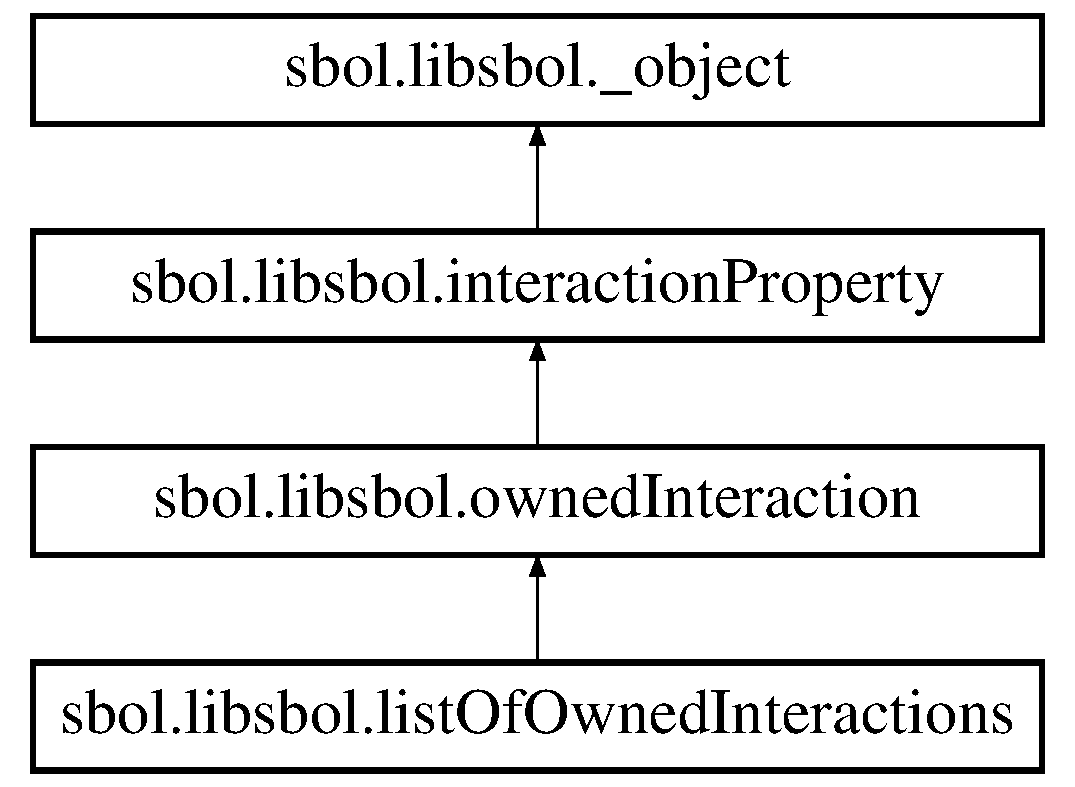
\includegraphics[height=4.000000cm]{classsbol_1_1libsbol_1_1owned_interaction}
\end{center}
\end{figure}
\subsection*{Public Member Functions}
\begin{DoxyCompactItemize}
\item 
def \hyperlink{classsbol_1_1libsbol_1_1owned_interaction_a1fd73dd73e932f39bd2d434fae75d62e}{\+\_\+\+\_\+init\+\_\+\+\_\+} (self, args)
\item 
def \hyperlink{classsbol_1_1libsbol_1_1owned_interaction_aee95e9bbec7e62f57f6379c046cfe7c3}{add} (self, sbol\+\_\+obj)
\item 
def \hyperlink{classsbol_1_1libsbol_1_1owned_interaction_a9ac119c77c8e9eba321e7952c1ba913d}{set} (self, sbol\+\_\+obj)
\item 
def \hyperlink{classsbol_1_1libsbol_1_1owned_interaction_af431ec537dc6cbd90b78a831bd344b0f}{get} (self, object\+\_\+id)
\item 
def \hyperlink{classsbol_1_1libsbol_1_1owned_interaction_ac2beb618e032e36265e223ddc674d9ae}{copy} (self)
\item 
def \hyperlink{classsbol_1_1libsbol_1_1owned_interaction_a155bc28610037adf2299dacda62a144a}{create} (self, args)
\item 
def \hyperlink{classsbol_1_1libsbol_1_1owned_interaction_a5ec343249635b63e7f20aeda75c2b97c}{begin} (self)
\item 
def \hyperlink{classsbol_1_1libsbol_1_1owned_interaction_a519f7d9830cea62b3279e2d536796e5c}{end} (self)
\item 
def {\bfseries size} (self)\hypertarget{classsbol_1_1libsbol_1_1owned_interaction_a8c2f5fb27ac8fd5bb8f134c7367720b1}{}\label{classsbol_1_1libsbol_1_1owned_interaction_a8c2f5fb27ac8fd5bb8f134c7367720b1}

\item 
def {\bfseries \+\_\+\+\_\+getitem\+\_\+\+\_\+} (self, args)\hypertarget{classsbol_1_1libsbol_1_1owned_interaction_a17d5aa55fd331a72b74cc60ff1148182}{}\label{classsbol_1_1libsbol_1_1owned_interaction_a17d5aa55fd331a72b74cc60ff1148182}

\item 
def {\bfseries \+\_\+\+\_\+iter\+\_\+\+\_\+} (self)\hypertarget{classsbol_1_1libsbol_1_1owned_interaction_abce76b28a03248007b2a3be935c68277}{}\label{classsbol_1_1libsbol_1_1owned_interaction_abce76b28a03248007b2a3be935c68277}

\item 
def {\bfseries next} (self)\hypertarget{classsbol_1_1libsbol_1_1owned_interaction_a7e10e06562e757d96190dfdd042f2045}{}\label{classsbol_1_1libsbol_1_1owned_interaction_a7e10e06562e757d96190dfdd042f2045}

\item 
def {\bfseries \+\_\+\+\_\+len\+\_\+\+\_\+} (self)\hypertarget{classsbol_1_1libsbol_1_1owned_interaction_a7a4e2fbbe8ab6c03fbcb9921e1f9402d}{}\label{classsbol_1_1libsbol_1_1owned_interaction_a7a4e2fbbe8ab6c03fbcb9921e1f9402d}

\item 
def \hyperlink{classsbol_1_1libsbol_1_1owned_interaction_a3250116cf795d573c83a5956d31d8a59}{add\+Range} (self, sbol\+\_\+obj)
\item 
def \hyperlink{classsbol_1_1libsbol_1_1owned_interaction_abeada70e3da6803590d55dc56bc94c08}{get\+Range} (self)
\end{DoxyCompactItemize}
\subsection*{Public Attributes}
\begin{DoxyCompactItemize}
\item 
{\bfseries this}\hypertarget{classsbol_1_1libsbol_1_1owned_interaction_a3ecf78fdddfb4adbc5f1acef7f5c2f20}{}\label{classsbol_1_1libsbol_1_1owned_interaction_a3ecf78fdddfb4adbc5f1acef7f5c2f20}

\end{DoxyCompactItemize}
\subsection*{Static Public Attributes}
\begin{DoxyCompactItemize}
\item 
{\bfseries python\+\_\+iter} = \+\_\+swig\+\_\+property(\+\_\+libsbol.\+owned\+Interaction\+\_\+python\+\_\+iter\+\_\+get, \+\_\+libsbol.\+owned\+Interaction\+\_\+python\+\_\+iter\+\_\+set)\hypertarget{classsbol_1_1libsbol_1_1owned_interaction_aa9b5f37c6567bb07861148ba62fc3a06}{}\label{classsbol_1_1libsbol_1_1owned_interaction_aa9b5f37c6567bb07861148ba62fc3a06}

\end{DoxyCompactItemize}


\subsection{Constructor \& Destructor Documentation}
\index{sbol\+::libsbol\+::owned\+Interaction@{sbol\+::libsbol\+::owned\+Interaction}!\+\_\+\+\_\+init\+\_\+\+\_\+@{\+\_\+\+\_\+init\+\_\+\+\_\+}}
\index{\+\_\+\+\_\+init\+\_\+\+\_\+@{\+\_\+\+\_\+init\+\_\+\+\_\+}!sbol\+::libsbol\+::owned\+Interaction@{sbol\+::libsbol\+::owned\+Interaction}}
\subsubsection[{\texorpdfstring{\+\_\+\+\_\+init\+\_\+\+\_\+(self, args)}{__init__(self, args)}}]{\setlength{\rightskip}{0pt plus 5cm}def sbol.\+libsbol.\+owned\+Interaction.\+\_\+\+\_\+init\+\_\+\+\_\+ (
\begin{DoxyParamCaption}
\item[{}]{self, }
\item[{}]{args}
\end{DoxyParamCaption}
)}\hypertarget{classsbol_1_1libsbol_1_1owned_interaction_a1fd73dd73e932f39bd2d434fae75d62e}{}\label{classsbol_1_1libsbol_1_1owned_interaction_a1fd73dd73e932f39bd2d434fae75d62e}
\begin{DoxyVerb}sbol::OwnedObject< SBOLClass >::OwnedObject(sbol_type type_uri, void
*property_owner, SBOLObject &first_object) 
\end{DoxyVerb}
 

\subsection{Member Function Documentation}
\index{sbol\+::libsbol\+::owned\+Interaction@{sbol\+::libsbol\+::owned\+Interaction}!add@{add}}
\index{add@{add}!sbol\+::libsbol\+::owned\+Interaction@{sbol\+::libsbol\+::owned\+Interaction}}
\subsubsection[{\texorpdfstring{add(self, sbol\+\_\+obj)}{add(self, sbol_obj)}}]{\setlength{\rightskip}{0pt plus 5cm}def sbol.\+libsbol.\+owned\+Interaction.\+add (
\begin{DoxyParamCaption}
\item[{}]{self, }
\item[{}]{sbol\+\_\+obj}
\end{DoxyParamCaption}
)}\hypertarget{classsbol_1_1libsbol_1_1owned_interaction_aee95e9bbec7e62f57f6379c046cfe7c3}{}\label{classsbol_1_1libsbol_1_1owned_interaction_aee95e9bbec7e62f57f6379c046cfe7c3}
\begin{DoxyVerb}void
sbol::OwnedObject< SBOLClass >::add(SBOLClass &sbol_obj) 
\end{DoxyVerb}
 \index{sbol\+::libsbol\+::owned\+Interaction@{sbol\+::libsbol\+::owned\+Interaction}!add\+Range@{add\+Range}}
\index{add\+Range@{add\+Range}!sbol\+::libsbol\+::owned\+Interaction@{sbol\+::libsbol\+::owned\+Interaction}}
\subsubsection[{\texorpdfstring{add\+Range(self, sbol\+\_\+obj)}{addRange(self, sbol_obj)}}]{\setlength{\rightskip}{0pt plus 5cm}def sbol.\+libsbol.\+owned\+Interaction.\+add\+Range (
\begin{DoxyParamCaption}
\item[{}]{self, }
\item[{}]{sbol\+\_\+obj}
\end{DoxyParamCaption}
)}\hypertarget{classsbol_1_1libsbol_1_1owned_interaction_a3250116cf795d573c83a5956d31d8a59}{}\label{classsbol_1_1libsbol_1_1owned_interaction_a3250116cf795d573c83a5956d31d8a59}
\begin{DoxyVerb}void
sbol::OwnedObject< SBOLClass >::add(SBOLClass &sbol_obj) 
\end{DoxyVerb}
 \index{sbol\+::libsbol\+::owned\+Interaction@{sbol\+::libsbol\+::owned\+Interaction}!begin@{begin}}
\index{begin@{begin}!sbol\+::libsbol\+::owned\+Interaction@{sbol\+::libsbol\+::owned\+Interaction}}
\subsubsection[{\texorpdfstring{begin(self)}{begin(self)}}]{\setlength{\rightskip}{0pt plus 5cm}def sbol.\+libsbol.\+owned\+Interaction.\+begin (
\begin{DoxyParamCaption}
\item[{}]{self}
\end{DoxyParamCaption}
)}\hypertarget{classsbol_1_1libsbol_1_1owned_interaction_a5ec343249635b63e7f20aeda75c2b97c}{}\label{classsbol_1_1libsbol_1_1owned_interaction_a5ec343249635b63e7f20aeda75c2b97c}
\begin{DoxyVerb}iterator
sbol::OwnedObject< SBOLClass >::begin() 
\end{DoxyVerb}
 \index{sbol\+::libsbol\+::owned\+Interaction@{sbol\+::libsbol\+::owned\+Interaction}!copy@{copy}}
\index{copy@{copy}!sbol\+::libsbol\+::owned\+Interaction@{sbol\+::libsbol\+::owned\+Interaction}}
\subsubsection[{\texorpdfstring{copy(self)}{copy(self)}}]{\setlength{\rightskip}{0pt plus 5cm}def sbol.\+libsbol.\+owned\+Interaction.\+copy (
\begin{DoxyParamCaption}
\item[{}]{self}
\end{DoxyParamCaption}
)}\hypertarget{classsbol_1_1libsbol_1_1owned_interaction_ac2beb618e032e36265e223ddc674d9ae}{}\label{classsbol_1_1libsbol_1_1owned_interaction_ac2beb618e032e36265e223ddc674d9ae}
\begin{DoxyVerb}std::vector<
SBOLClass * > sbol::OwnedObject< SBOLClass >::copy() 
\end{DoxyVerb}
 \index{sbol\+::libsbol\+::owned\+Interaction@{sbol\+::libsbol\+::owned\+Interaction}!create@{create}}
\index{create@{create}!sbol\+::libsbol\+::owned\+Interaction@{sbol\+::libsbol\+::owned\+Interaction}}
\subsubsection[{\texorpdfstring{create(self, args)}{create(self, args)}}]{\setlength{\rightskip}{0pt plus 5cm}def sbol.\+libsbol.\+owned\+Interaction.\+create (
\begin{DoxyParamCaption}
\item[{}]{self, }
\item[{}]{args}
\end{DoxyParamCaption}
)}\hypertarget{classsbol_1_1libsbol_1_1owned_interaction_a155bc28610037adf2299dacda62a144a}{}\label{classsbol_1_1libsbol_1_1owned_interaction_a155bc28610037adf2299dacda62a144a}
\begin{DoxyVerb}void
sbol::OwnedObject< SBOLClass >::create(std::string uri_prefix,
std::string display_id, std::string version) 
\end{DoxyVerb}
 \index{sbol\+::libsbol\+::owned\+Interaction@{sbol\+::libsbol\+::owned\+Interaction}!end@{end}}
\index{end@{end}!sbol\+::libsbol\+::owned\+Interaction@{sbol\+::libsbol\+::owned\+Interaction}}
\subsubsection[{\texorpdfstring{end(self)}{end(self)}}]{\setlength{\rightskip}{0pt plus 5cm}def sbol.\+libsbol.\+owned\+Interaction.\+end (
\begin{DoxyParamCaption}
\item[{}]{self}
\end{DoxyParamCaption}
)}\hypertarget{classsbol_1_1libsbol_1_1owned_interaction_a519f7d9830cea62b3279e2d536796e5c}{}\label{classsbol_1_1libsbol_1_1owned_interaction_a519f7d9830cea62b3279e2d536796e5c}
\begin{DoxyVerb}iterator
sbol::OwnedObject< SBOLClass >::end() 
\end{DoxyVerb}
 \index{sbol\+::libsbol\+::owned\+Interaction@{sbol\+::libsbol\+::owned\+Interaction}!get@{get}}
\index{get@{get}!sbol\+::libsbol\+::owned\+Interaction@{sbol\+::libsbol\+::owned\+Interaction}}
\subsubsection[{\texorpdfstring{get(self, object\+\_\+id)}{get(self, object_id)}}]{\setlength{\rightskip}{0pt plus 5cm}def sbol.\+libsbol.\+owned\+Interaction.\+get (
\begin{DoxyParamCaption}
\item[{}]{self, }
\item[{}]{object\+\_\+id}
\end{DoxyParamCaption}
)}\hypertarget{classsbol_1_1libsbol_1_1owned_interaction_af431ec537dc6cbd90b78a831bd344b0f}{}\label{classsbol_1_1libsbol_1_1owned_interaction_af431ec537dc6cbd90b78a831bd344b0f}
\begin{DoxyVerb}SBOLClass &
sbol::OwnedObject< SBOLClass >::get(const std::string object_id) 
\end{DoxyVerb}
 \index{sbol\+::libsbol\+::owned\+Interaction@{sbol\+::libsbol\+::owned\+Interaction}!get\+Range@{get\+Range}}
\index{get\+Range@{get\+Range}!sbol\+::libsbol\+::owned\+Interaction@{sbol\+::libsbol\+::owned\+Interaction}}
\subsubsection[{\texorpdfstring{get\+Range(self)}{getRange(self)}}]{\setlength{\rightskip}{0pt plus 5cm}def sbol.\+libsbol.\+owned\+Interaction.\+get\+Range (
\begin{DoxyParamCaption}
\item[{}]{self}
\end{DoxyParamCaption}
)}\hypertarget{classsbol_1_1libsbol_1_1owned_interaction_abeada70e3da6803590d55dc56bc94c08}{}\label{classsbol_1_1libsbol_1_1owned_interaction_abeada70e3da6803590d55dc56bc94c08}
\begin{DoxyVerb}SBOLClass &
sbol::OwnedObject< SBOLClass >::get(const std::string object_id) 
\end{DoxyVerb}
 \index{sbol\+::libsbol\+::owned\+Interaction@{sbol\+::libsbol\+::owned\+Interaction}!set@{set}}
\index{set@{set}!sbol\+::libsbol\+::owned\+Interaction@{sbol\+::libsbol\+::owned\+Interaction}}
\subsubsection[{\texorpdfstring{set(self, sbol\+\_\+obj)}{set(self, sbol_obj)}}]{\setlength{\rightskip}{0pt plus 5cm}def sbol.\+libsbol.\+owned\+Interaction.\+set (
\begin{DoxyParamCaption}
\item[{}]{self, }
\item[{}]{sbol\+\_\+obj}
\end{DoxyParamCaption}
)}\hypertarget{classsbol_1_1libsbol_1_1owned_interaction_a9ac119c77c8e9eba321e7952c1ba913d}{}\label{classsbol_1_1libsbol_1_1owned_interaction_a9ac119c77c8e9eba321e7952c1ba913d}
\begin{DoxyVerb}void
sbol::OwnedObject< SBOLClass >::set(SBOLClass &sbol_obj) 
\end{DoxyVerb}
 

The documentation for this class was generated from the following file\+:\begin{DoxyCompactItemize}
\item 
libsbol.\+py\end{DoxyCompactItemize}

\hypertarget{classsbol_1_1libsbol_1_1owned_maps_to}{}\section{sbol.\+libsbol.\+owned\+Maps\+To Class Reference}
\label{classsbol_1_1libsbol_1_1owned_maps_to}\index{sbol.\+libsbol.\+owned\+Maps\+To@{sbol.\+libsbol.\+owned\+Maps\+To}}
Inheritance diagram for sbol.\+libsbol.\+owned\+Maps\+To\+:\begin{figure}[H]
\begin{center}
\leavevmode
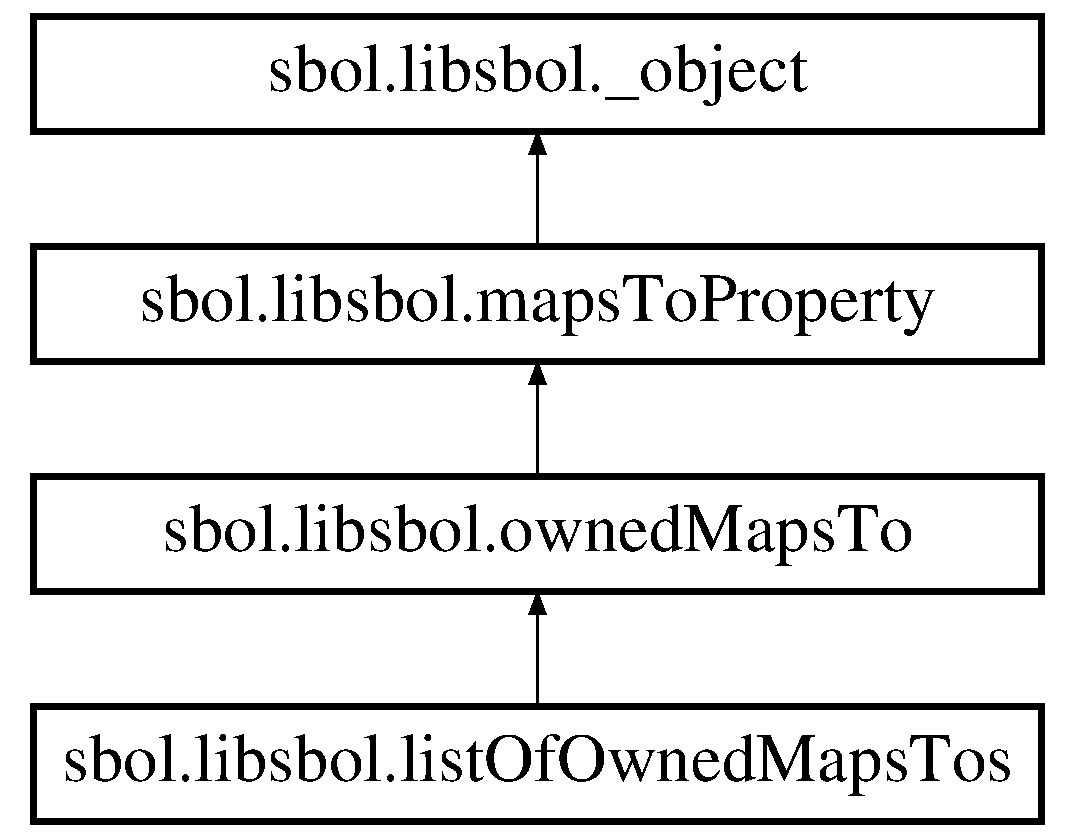
\includegraphics[height=4.000000cm]{classsbol_1_1libsbol_1_1owned_maps_to}
\end{center}
\end{figure}
\subsection*{Public Member Functions}
\begin{DoxyCompactItemize}
\item 
def \hyperlink{classsbol_1_1libsbol_1_1owned_maps_to_a30b6abfd354d7ca02ec3e8c72d8f0275}{\+\_\+\+\_\+init\+\_\+\+\_\+} (self, args)
\item 
def \hyperlink{classsbol_1_1libsbol_1_1owned_maps_to_a64db1699ec1f7e1d3a6d8214e6208bbc}{add} (self, sbol\+\_\+obj)
\item 
def \hyperlink{classsbol_1_1libsbol_1_1owned_maps_to_a82ec21fc5984fdd28a283fa1cab6225e}{set} (self, sbol\+\_\+obj)
\item 
def \hyperlink{classsbol_1_1libsbol_1_1owned_maps_to_a149abdcd72a0358a509d0342c67cafb7}{get} (self, object\+\_\+id)
\item 
def \hyperlink{classsbol_1_1libsbol_1_1owned_maps_to_ad92c424f609eafc711c2785d739f5588}{copy} (self)
\item 
def \hyperlink{classsbol_1_1libsbol_1_1owned_maps_to_a6a1eabad8ca37e7ede96ce39072bfb3f}{create} (self, args)
\item 
def \hyperlink{classsbol_1_1libsbol_1_1owned_maps_to_a585f7d61ff5b45460015daa139546976}{begin} (self)
\item 
def \hyperlink{classsbol_1_1libsbol_1_1owned_maps_to_a3c4ef7b0c0fa82e91764dc8da31fd149}{end} (self)
\item 
def {\bfseries size} (self)\hypertarget{classsbol_1_1libsbol_1_1owned_maps_to_abbcc15f091c0332ad46c2192c5ce9f98}{}\label{classsbol_1_1libsbol_1_1owned_maps_to_abbcc15f091c0332ad46c2192c5ce9f98}

\item 
def {\bfseries \+\_\+\+\_\+getitem\+\_\+\+\_\+} (self, args)\hypertarget{classsbol_1_1libsbol_1_1owned_maps_to_af42f2acc71eb490e7d7047e1880a4b5e}{}\label{classsbol_1_1libsbol_1_1owned_maps_to_af42f2acc71eb490e7d7047e1880a4b5e}

\item 
def {\bfseries \+\_\+\+\_\+iter\+\_\+\+\_\+} (self)\hypertarget{classsbol_1_1libsbol_1_1owned_maps_to_af248d860b74116f5bba462dc551db375}{}\label{classsbol_1_1libsbol_1_1owned_maps_to_af248d860b74116f5bba462dc551db375}

\item 
def {\bfseries next} (self)\hypertarget{classsbol_1_1libsbol_1_1owned_maps_to_ae4c30dde7a22dbb142b37db2220d11b3}{}\label{classsbol_1_1libsbol_1_1owned_maps_to_ae4c30dde7a22dbb142b37db2220d11b3}

\item 
def {\bfseries \+\_\+\+\_\+len\+\_\+\+\_\+} (self)\hypertarget{classsbol_1_1libsbol_1_1owned_maps_to_a1d292de3e1257f4b6f61805157db5eea}{}\label{classsbol_1_1libsbol_1_1owned_maps_to_a1d292de3e1257f4b6f61805157db5eea}

\item 
def \hyperlink{classsbol_1_1libsbol_1_1owned_maps_to_ae2dd505bc080233a9f3d1bb687493142}{add\+Range} (self, sbol\+\_\+obj)
\item 
def \hyperlink{classsbol_1_1libsbol_1_1owned_maps_to_ae188785c2b7b1261e52b3417286aa454}{get\+Range} (self)
\end{DoxyCompactItemize}
\subsection*{Public Attributes}
\begin{DoxyCompactItemize}
\item 
{\bfseries this}\hypertarget{classsbol_1_1libsbol_1_1owned_maps_to_ad5f06ca20294a6e1197915ed308b575b}{}\label{classsbol_1_1libsbol_1_1owned_maps_to_ad5f06ca20294a6e1197915ed308b575b}

\end{DoxyCompactItemize}
\subsection*{Static Public Attributes}
\begin{DoxyCompactItemize}
\item 
{\bfseries python\+\_\+iter} = \+\_\+swig\+\_\+property(\+\_\+libsbol.\+owned\+Maps\+To\+\_\+python\+\_\+iter\+\_\+get, \+\_\+libsbol.\+owned\+Maps\+To\+\_\+python\+\_\+iter\+\_\+set)\hypertarget{classsbol_1_1libsbol_1_1owned_maps_to_ade430632d54465a144b7e13b7a3af670}{}\label{classsbol_1_1libsbol_1_1owned_maps_to_ade430632d54465a144b7e13b7a3af670}

\end{DoxyCompactItemize}


\subsection{Constructor \& Destructor Documentation}
\index{sbol\+::libsbol\+::owned\+Maps\+To@{sbol\+::libsbol\+::owned\+Maps\+To}!\+\_\+\+\_\+init\+\_\+\+\_\+@{\+\_\+\+\_\+init\+\_\+\+\_\+}}
\index{\+\_\+\+\_\+init\+\_\+\+\_\+@{\+\_\+\+\_\+init\+\_\+\+\_\+}!sbol\+::libsbol\+::owned\+Maps\+To@{sbol\+::libsbol\+::owned\+Maps\+To}}
\subsubsection[{\texorpdfstring{\+\_\+\+\_\+init\+\_\+\+\_\+(self, args)}{__init__(self, args)}}]{\setlength{\rightskip}{0pt plus 5cm}def sbol.\+libsbol.\+owned\+Maps\+To.\+\_\+\+\_\+init\+\_\+\+\_\+ (
\begin{DoxyParamCaption}
\item[{}]{self, }
\item[{}]{args}
\end{DoxyParamCaption}
)}\hypertarget{classsbol_1_1libsbol_1_1owned_maps_to_a30b6abfd354d7ca02ec3e8c72d8f0275}{}\label{classsbol_1_1libsbol_1_1owned_maps_to_a30b6abfd354d7ca02ec3e8c72d8f0275}
\begin{DoxyVerb}sbol::OwnedObject< SBOLClass >::OwnedObject(sbol_type type_uri, void
*property_owner, SBOLObject &first_object) 
\end{DoxyVerb}
 

\subsection{Member Function Documentation}
\index{sbol\+::libsbol\+::owned\+Maps\+To@{sbol\+::libsbol\+::owned\+Maps\+To}!add@{add}}
\index{add@{add}!sbol\+::libsbol\+::owned\+Maps\+To@{sbol\+::libsbol\+::owned\+Maps\+To}}
\subsubsection[{\texorpdfstring{add(self, sbol\+\_\+obj)}{add(self, sbol_obj)}}]{\setlength{\rightskip}{0pt plus 5cm}def sbol.\+libsbol.\+owned\+Maps\+To.\+add (
\begin{DoxyParamCaption}
\item[{}]{self, }
\item[{}]{sbol\+\_\+obj}
\end{DoxyParamCaption}
)}\hypertarget{classsbol_1_1libsbol_1_1owned_maps_to_a64db1699ec1f7e1d3a6d8214e6208bbc}{}\label{classsbol_1_1libsbol_1_1owned_maps_to_a64db1699ec1f7e1d3a6d8214e6208bbc}
\begin{DoxyVerb}void
sbol::OwnedObject< SBOLClass >::add(SBOLClass &sbol_obj) 
\end{DoxyVerb}
 \index{sbol\+::libsbol\+::owned\+Maps\+To@{sbol\+::libsbol\+::owned\+Maps\+To}!add\+Range@{add\+Range}}
\index{add\+Range@{add\+Range}!sbol\+::libsbol\+::owned\+Maps\+To@{sbol\+::libsbol\+::owned\+Maps\+To}}
\subsubsection[{\texorpdfstring{add\+Range(self, sbol\+\_\+obj)}{addRange(self, sbol_obj)}}]{\setlength{\rightskip}{0pt plus 5cm}def sbol.\+libsbol.\+owned\+Maps\+To.\+add\+Range (
\begin{DoxyParamCaption}
\item[{}]{self, }
\item[{}]{sbol\+\_\+obj}
\end{DoxyParamCaption}
)}\hypertarget{classsbol_1_1libsbol_1_1owned_maps_to_ae2dd505bc080233a9f3d1bb687493142}{}\label{classsbol_1_1libsbol_1_1owned_maps_to_ae2dd505bc080233a9f3d1bb687493142}
\begin{DoxyVerb}void
sbol::OwnedObject< SBOLClass >::add(SBOLClass &sbol_obj) 
\end{DoxyVerb}
 \index{sbol\+::libsbol\+::owned\+Maps\+To@{sbol\+::libsbol\+::owned\+Maps\+To}!begin@{begin}}
\index{begin@{begin}!sbol\+::libsbol\+::owned\+Maps\+To@{sbol\+::libsbol\+::owned\+Maps\+To}}
\subsubsection[{\texorpdfstring{begin(self)}{begin(self)}}]{\setlength{\rightskip}{0pt plus 5cm}def sbol.\+libsbol.\+owned\+Maps\+To.\+begin (
\begin{DoxyParamCaption}
\item[{}]{self}
\end{DoxyParamCaption}
)}\hypertarget{classsbol_1_1libsbol_1_1owned_maps_to_a585f7d61ff5b45460015daa139546976}{}\label{classsbol_1_1libsbol_1_1owned_maps_to_a585f7d61ff5b45460015daa139546976}
\begin{DoxyVerb}iterator
sbol::OwnedObject< SBOLClass >::begin() 
\end{DoxyVerb}
 \index{sbol\+::libsbol\+::owned\+Maps\+To@{sbol\+::libsbol\+::owned\+Maps\+To}!copy@{copy}}
\index{copy@{copy}!sbol\+::libsbol\+::owned\+Maps\+To@{sbol\+::libsbol\+::owned\+Maps\+To}}
\subsubsection[{\texorpdfstring{copy(self)}{copy(self)}}]{\setlength{\rightskip}{0pt plus 5cm}def sbol.\+libsbol.\+owned\+Maps\+To.\+copy (
\begin{DoxyParamCaption}
\item[{}]{self}
\end{DoxyParamCaption}
)}\hypertarget{classsbol_1_1libsbol_1_1owned_maps_to_ad92c424f609eafc711c2785d739f5588}{}\label{classsbol_1_1libsbol_1_1owned_maps_to_ad92c424f609eafc711c2785d739f5588}
\begin{DoxyVerb}std::vector<
SBOLClass * > sbol::OwnedObject< SBOLClass >::copy() 
\end{DoxyVerb}
 \index{sbol\+::libsbol\+::owned\+Maps\+To@{sbol\+::libsbol\+::owned\+Maps\+To}!create@{create}}
\index{create@{create}!sbol\+::libsbol\+::owned\+Maps\+To@{sbol\+::libsbol\+::owned\+Maps\+To}}
\subsubsection[{\texorpdfstring{create(self, args)}{create(self, args)}}]{\setlength{\rightskip}{0pt plus 5cm}def sbol.\+libsbol.\+owned\+Maps\+To.\+create (
\begin{DoxyParamCaption}
\item[{}]{self, }
\item[{}]{args}
\end{DoxyParamCaption}
)}\hypertarget{classsbol_1_1libsbol_1_1owned_maps_to_a6a1eabad8ca37e7ede96ce39072bfb3f}{}\label{classsbol_1_1libsbol_1_1owned_maps_to_a6a1eabad8ca37e7ede96ce39072bfb3f}
\begin{DoxyVerb}void
sbol::OwnedObject< SBOLClass >::create(std::string uri_prefix,
std::string display_id, std::string version) 
\end{DoxyVerb}
 \index{sbol\+::libsbol\+::owned\+Maps\+To@{sbol\+::libsbol\+::owned\+Maps\+To}!end@{end}}
\index{end@{end}!sbol\+::libsbol\+::owned\+Maps\+To@{sbol\+::libsbol\+::owned\+Maps\+To}}
\subsubsection[{\texorpdfstring{end(self)}{end(self)}}]{\setlength{\rightskip}{0pt plus 5cm}def sbol.\+libsbol.\+owned\+Maps\+To.\+end (
\begin{DoxyParamCaption}
\item[{}]{self}
\end{DoxyParamCaption}
)}\hypertarget{classsbol_1_1libsbol_1_1owned_maps_to_a3c4ef7b0c0fa82e91764dc8da31fd149}{}\label{classsbol_1_1libsbol_1_1owned_maps_to_a3c4ef7b0c0fa82e91764dc8da31fd149}
\begin{DoxyVerb}iterator
sbol::OwnedObject< SBOLClass >::end() 
\end{DoxyVerb}
 \index{sbol\+::libsbol\+::owned\+Maps\+To@{sbol\+::libsbol\+::owned\+Maps\+To}!get@{get}}
\index{get@{get}!sbol\+::libsbol\+::owned\+Maps\+To@{sbol\+::libsbol\+::owned\+Maps\+To}}
\subsubsection[{\texorpdfstring{get(self, object\+\_\+id)}{get(self, object_id)}}]{\setlength{\rightskip}{0pt plus 5cm}def sbol.\+libsbol.\+owned\+Maps\+To.\+get (
\begin{DoxyParamCaption}
\item[{}]{self, }
\item[{}]{object\+\_\+id}
\end{DoxyParamCaption}
)}\hypertarget{classsbol_1_1libsbol_1_1owned_maps_to_a149abdcd72a0358a509d0342c67cafb7}{}\label{classsbol_1_1libsbol_1_1owned_maps_to_a149abdcd72a0358a509d0342c67cafb7}
\begin{DoxyVerb}SBOLClass &
sbol::OwnedObject< SBOLClass >::get(const std::string object_id) 
\end{DoxyVerb}
 \index{sbol\+::libsbol\+::owned\+Maps\+To@{sbol\+::libsbol\+::owned\+Maps\+To}!get\+Range@{get\+Range}}
\index{get\+Range@{get\+Range}!sbol\+::libsbol\+::owned\+Maps\+To@{sbol\+::libsbol\+::owned\+Maps\+To}}
\subsubsection[{\texorpdfstring{get\+Range(self)}{getRange(self)}}]{\setlength{\rightskip}{0pt plus 5cm}def sbol.\+libsbol.\+owned\+Maps\+To.\+get\+Range (
\begin{DoxyParamCaption}
\item[{}]{self}
\end{DoxyParamCaption}
)}\hypertarget{classsbol_1_1libsbol_1_1owned_maps_to_ae188785c2b7b1261e52b3417286aa454}{}\label{classsbol_1_1libsbol_1_1owned_maps_to_ae188785c2b7b1261e52b3417286aa454}
\begin{DoxyVerb}SBOLClass &
sbol::OwnedObject< SBOLClass >::get(const std::string object_id) 
\end{DoxyVerb}
 \index{sbol\+::libsbol\+::owned\+Maps\+To@{sbol\+::libsbol\+::owned\+Maps\+To}!set@{set}}
\index{set@{set}!sbol\+::libsbol\+::owned\+Maps\+To@{sbol\+::libsbol\+::owned\+Maps\+To}}
\subsubsection[{\texorpdfstring{set(self, sbol\+\_\+obj)}{set(self, sbol_obj)}}]{\setlength{\rightskip}{0pt plus 5cm}def sbol.\+libsbol.\+owned\+Maps\+To.\+set (
\begin{DoxyParamCaption}
\item[{}]{self, }
\item[{}]{sbol\+\_\+obj}
\end{DoxyParamCaption}
)}\hypertarget{classsbol_1_1libsbol_1_1owned_maps_to_a82ec21fc5984fdd28a283fa1cab6225e}{}\label{classsbol_1_1libsbol_1_1owned_maps_to_a82ec21fc5984fdd28a283fa1cab6225e}
\begin{DoxyVerb}void
sbol::OwnedObject< SBOLClass >::set(SBOLClass &sbol_obj) 
\end{DoxyVerb}
 

The documentation for this class was generated from the following file\+:\begin{DoxyCompactItemize}
\item 
libsbol.\+py\end{DoxyCompactItemize}

\hypertarget{classsbol_1_1libsbol_1_1owned_module}{}\section{sbol.\+libsbol.\+owned\+Module Class Reference}
\label{classsbol_1_1libsbol_1_1owned_module}\index{sbol.\+libsbol.\+owned\+Module@{sbol.\+libsbol.\+owned\+Module}}
Inheritance diagram for sbol.\+libsbol.\+owned\+Module\+:\begin{figure}[H]
\begin{center}
\leavevmode
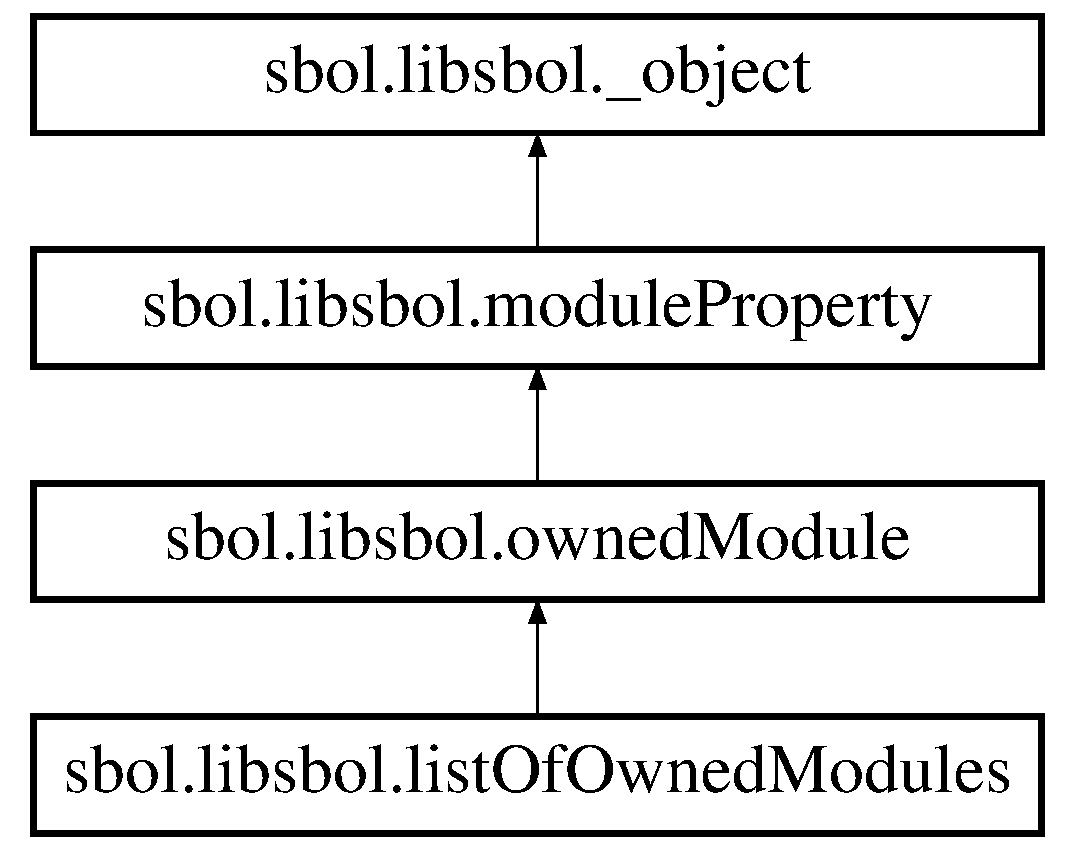
\includegraphics[height=4.000000cm]{classsbol_1_1libsbol_1_1owned_module}
\end{center}
\end{figure}
\subsection*{Public Member Functions}
\begin{DoxyCompactItemize}
\item 
def \hyperlink{classsbol_1_1libsbol_1_1owned_module_a7b7efdff6b927ce613bb74034c490993}{\+\_\+\+\_\+init\+\_\+\+\_\+} (self, args)
\item 
def \hyperlink{classsbol_1_1libsbol_1_1owned_module_ae2472562038d9929b4e5ed56da68dc41}{add} (self, sbol\+\_\+obj)
\item 
def \hyperlink{classsbol_1_1libsbol_1_1owned_module_a39a01397e3429fc60eaa5ff356ed3272}{set} (self, sbol\+\_\+obj)
\item 
def \hyperlink{classsbol_1_1libsbol_1_1owned_module_af5f37e53a9cd3cb257328ec51aabd3d7}{get} (self, object\+\_\+id)
\item 
def \hyperlink{classsbol_1_1libsbol_1_1owned_module_ad69e345145bd60b9de3fdcd0375b36ea}{copy} (self)
\item 
def \hyperlink{classsbol_1_1libsbol_1_1owned_module_a1ab74713732b4d37abb8ec67ffa98143}{create} (self, args)
\item 
def \hyperlink{classsbol_1_1libsbol_1_1owned_module_a7d1bce303907e19c090fd915e4c41ee7}{begin} (self)
\item 
def \hyperlink{classsbol_1_1libsbol_1_1owned_module_a25abde762b1e941079d7ae4ba0a90c53}{end} (self)
\item 
def {\bfseries size} (self)\hypertarget{classsbol_1_1libsbol_1_1owned_module_a774b565549fd59ef4fdf12f62465dea1}{}\label{classsbol_1_1libsbol_1_1owned_module_a774b565549fd59ef4fdf12f62465dea1}

\item 
def {\bfseries \+\_\+\+\_\+getitem\+\_\+\+\_\+} (self, args)\hypertarget{classsbol_1_1libsbol_1_1owned_module_a3c70bd3da2d0ee19f3d09e2f6418eb8d}{}\label{classsbol_1_1libsbol_1_1owned_module_a3c70bd3da2d0ee19f3d09e2f6418eb8d}

\item 
def {\bfseries \+\_\+\+\_\+iter\+\_\+\+\_\+} (self)\hypertarget{classsbol_1_1libsbol_1_1owned_module_a066fa224a56ca958a730bf3d67205898}{}\label{classsbol_1_1libsbol_1_1owned_module_a066fa224a56ca958a730bf3d67205898}

\item 
def {\bfseries next} (self)\hypertarget{classsbol_1_1libsbol_1_1owned_module_a912d31f9bc2eb9f69c7cd2657c729266}{}\label{classsbol_1_1libsbol_1_1owned_module_a912d31f9bc2eb9f69c7cd2657c729266}

\item 
def {\bfseries \+\_\+\+\_\+len\+\_\+\+\_\+} (self)\hypertarget{classsbol_1_1libsbol_1_1owned_module_a9548ca13b2064cc3f5c4bd0426a8cd04}{}\label{classsbol_1_1libsbol_1_1owned_module_a9548ca13b2064cc3f5c4bd0426a8cd04}

\item 
def \hyperlink{classsbol_1_1libsbol_1_1owned_module_af337fdebd37abea375b7f18f9d8b4191}{add\+Range} (self, sbol\+\_\+obj)
\item 
def \hyperlink{classsbol_1_1libsbol_1_1owned_module_a4fbef4adc3046944efc15c7807996194}{get\+Range} (self)
\end{DoxyCompactItemize}
\subsection*{Public Attributes}
\begin{DoxyCompactItemize}
\item 
{\bfseries this}\hypertarget{classsbol_1_1libsbol_1_1owned_module_ad06be5ee9dbdb5a349366f9fdebe6d8c}{}\label{classsbol_1_1libsbol_1_1owned_module_ad06be5ee9dbdb5a349366f9fdebe6d8c}

\end{DoxyCompactItemize}
\subsection*{Static Public Attributes}
\begin{DoxyCompactItemize}
\item 
{\bfseries python\+\_\+iter} = \+\_\+swig\+\_\+property(\+\_\+libsbol.\+owned\+Module\+\_\+python\+\_\+iter\+\_\+get, \+\_\+libsbol.\+owned\+Module\+\_\+python\+\_\+iter\+\_\+set)\hypertarget{classsbol_1_1libsbol_1_1owned_module_a3f6eb7e38767b7b49ac0a96b9316ce68}{}\label{classsbol_1_1libsbol_1_1owned_module_a3f6eb7e38767b7b49ac0a96b9316ce68}

\end{DoxyCompactItemize}


\subsection{Constructor \& Destructor Documentation}
\index{sbol\+::libsbol\+::owned\+Module@{sbol\+::libsbol\+::owned\+Module}!\+\_\+\+\_\+init\+\_\+\+\_\+@{\+\_\+\+\_\+init\+\_\+\+\_\+}}
\index{\+\_\+\+\_\+init\+\_\+\+\_\+@{\+\_\+\+\_\+init\+\_\+\+\_\+}!sbol\+::libsbol\+::owned\+Module@{sbol\+::libsbol\+::owned\+Module}}
\subsubsection[{\texorpdfstring{\+\_\+\+\_\+init\+\_\+\+\_\+(self, args)}{__init__(self, args)}}]{\setlength{\rightskip}{0pt plus 5cm}def sbol.\+libsbol.\+owned\+Module.\+\_\+\+\_\+init\+\_\+\+\_\+ (
\begin{DoxyParamCaption}
\item[{}]{self, }
\item[{}]{args}
\end{DoxyParamCaption}
)}\hypertarget{classsbol_1_1libsbol_1_1owned_module_a7b7efdff6b927ce613bb74034c490993}{}\label{classsbol_1_1libsbol_1_1owned_module_a7b7efdff6b927ce613bb74034c490993}
\begin{DoxyVerb}sbol::OwnedObject< SBOLClass >::OwnedObject(sbol_type type_uri, void
*property_owner, SBOLObject &first_object) 
\end{DoxyVerb}
 

\subsection{Member Function Documentation}
\index{sbol\+::libsbol\+::owned\+Module@{sbol\+::libsbol\+::owned\+Module}!add@{add}}
\index{add@{add}!sbol\+::libsbol\+::owned\+Module@{sbol\+::libsbol\+::owned\+Module}}
\subsubsection[{\texorpdfstring{add(self, sbol\+\_\+obj)}{add(self, sbol_obj)}}]{\setlength{\rightskip}{0pt plus 5cm}def sbol.\+libsbol.\+owned\+Module.\+add (
\begin{DoxyParamCaption}
\item[{}]{self, }
\item[{}]{sbol\+\_\+obj}
\end{DoxyParamCaption}
)}\hypertarget{classsbol_1_1libsbol_1_1owned_module_ae2472562038d9929b4e5ed56da68dc41}{}\label{classsbol_1_1libsbol_1_1owned_module_ae2472562038d9929b4e5ed56da68dc41}
\begin{DoxyVerb}void
sbol::OwnedObject< SBOLClass >::add(SBOLClass &sbol_obj) 
\end{DoxyVerb}
 \index{sbol\+::libsbol\+::owned\+Module@{sbol\+::libsbol\+::owned\+Module}!add\+Range@{add\+Range}}
\index{add\+Range@{add\+Range}!sbol\+::libsbol\+::owned\+Module@{sbol\+::libsbol\+::owned\+Module}}
\subsubsection[{\texorpdfstring{add\+Range(self, sbol\+\_\+obj)}{addRange(self, sbol_obj)}}]{\setlength{\rightskip}{0pt plus 5cm}def sbol.\+libsbol.\+owned\+Module.\+add\+Range (
\begin{DoxyParamCaption}
\item[{}]{self, }
\item[{}]{sbol\+\_\+obj}
\end{DoxyParamCaption}
)}\hypertarget{classsbol_1_1libsbol_1_1owned_module_af337fdebd37abea375b7f18f9d8b4191}{}\label{classsbol_1_1libsbol_1_1owned_module_af337fdebd37abea375b7f18f9d8b4191}
\begin{DoxyVerb}void
sbol::OwnedObject< SBOLClass >::add(SBOLClass &sbol_obj) 
\end{DoxyVerb}
 \index{sbol\+::libsbol\+::owned\+Module@{sbol\+::libsbol\+::owned\+Module}!begin@{begin}}
\index{begin@{begin}!sbol\+::libsbol\+::owned\+Module@{sbol\+::libsbol\+::owned\+Module}}
\subsubsection[{\texorpdfstring{begin(self)}{begin(self)}}]{\setlength{\rightskip}{0pt plus 5cm}def sbol.\+libsbol.\+owned\+Module.\+begin (
\begin{DoxyParamCaption}
\item[{}]{self}
\end{DoxyParamCaption}
)}\hypertarget{classsbol_1_1libsbol_1_1owned_module_a7d1bce303907e19c090fd915e4c41ee7}{}\label{classsbol_1_1libsbol_1_1owned_module_a7d1bce303907e19c090fd915e4c41ee7}
\begin{DoxyVerb}iterator
sbol::OwnedObject< SBOLClass >::begin() 
\end{DoxyVerb}
 \index{sbol\+::libsbol\+::owned\+Module@{sbol\+::libsbol\+::owned\+Module}!copy@{copy}}
\index{copy@{copy}!sbol\+::libsbol\+::owned\+Module@{sbol\+::libsbol\+::owned\+Module}}
\subsubsection[{\texorpdfstring{copy(self)}{copy(self)}}]{\setlength{\rightskip}{0pt plus 5cm}def sbol.\+libsbol.\+owned\+Module.\+copy (
\begin{DoxyParamCaption}
\item[{}]{self}
\end{DoxyParamCaption}
)}\hypertarget{classsbol_1_1libsbol_1_1owned_module_ad69e345145bd60b9de3fdcd0375b36ea}{}\label{classsbol_1_1libsbol_1_1owned_module_ad69e345145bd60b9de3fdcd0375b36ea}
\begin{DoxyVerb}std::vector<
SBOLClass * > sbol::OwnedObject< SBOLClass >::copy() 
\end{DoxyVerb}
 \index{sbol\+::libsbol\+::owned\+Module@{sbol\+::libsbol\+::owned\+Module}!create@{create}}
\index{create@{create}!sbol\+::libsbol\+::owned\+Module@{sbol\+::libsbol\+::owned\+Module}}
\subsubsection[{\texorpdfstring{create(self, args)}{create(self, args)}}]{\setlength{\rightskip}{0pt plus 5cm}def sbol.\+libsbol.\+owned\+Module.\+create (
\begin{DoxyParamCaption}
\item[{}]{self, }
\item[{}]{args}
\end{DoxyParamCaption}
)}\hypertarget{classsbol_1_1libsbol_1_1owned_module_a1ab74713732b4d37abb8ec67ffa98143}{}\label{classsbol_1_1libsbol_1_1owned_module_a1ab74713732b4d37abb8ec67ffa98143}
\begin{DoxyVerb}void
sbol::OwnedObject< SBOLClass >::create(std::string uri_prefix,
std::string display_id, std::string version) 
\end{DoxyVerb}
 \index{sbol\+::libsbol\+::owned\+Module@{sbol\+::libsbol\+::owned\+Module}!end@{end}}
\index{end@{end}!sbol\+::libsbol\+::owned\+Module@{sbol\+::libsbol\+::owned\+Module}}
\subsubsection[{\texorpdfstring{end(self)}{end(self)}}]{\setlength{\rightskip}{0pt plus 5cm}def sbol.\+libsbol.\+owned\+Module.\+end (
\begin{DoxyParamCaption}
\item[{}]{self}
\end{DoxyParamCaption}
)}\hypertarget{classsbol_1_1libsbol_1_1owned_module_a25abde762b1e941079d7ae4ba0a90c53}{}\label{classsbol_1_1libsbol_1_1owned_module_a25abde762b1e941079d7ae4ba0a90c53}
\begin{DoxyVerb}iterator
sbol::OwnedObject< SBOLClass >::end() 
\end{DoxyVerb}
 \index{sbol\+::libsbol\+::owned\+Module@{sbol\+::libsbol\+::owned\+Module}!get@{get}}
\index{get@{get}!sbol\+::libsbol\+::owned\+Module@{sbol\+::libsbol\+::owned\+Module}}
\subsubsection[{\texorpdfstring{get(self, object\+\_\+id)}{get(self, object_id)}}]{\setlength{\rightskip}{0pt plus 5cm}def sbol.\+libsbol.\+owned\+Module.\+get (
\begin{DoxyParamCaption}
\item[{}]{self, }
\item[{}]{object\+\_\+id}
\end{DoxyParamCaption}
)}\hypertarget{classsbol_1_1libsbol_1_1owned_module_af5f37e53a9cd3cb257328ec51aabd3d7}{}\label{classsbol_1_1libsbol_1_1owned_module_af5f37e53a9cd3cb257328ec51aabd3d7}
\begin{DoxyVerb}SBOLClass &
sbol::OwnedObject< SBOLClass >::get(const std::string object_id) 
\end{DoxyVerb}
 \index{sbol\+::libsbol\+::owned\+Module@{sbol\+::libsbol\+::owned\+Module}!get\+Range@{get\+Range}}
\index{get\+Range@{get\+Range}!sbol\+::libsbol\+::owned\+Module@{sbol\+::libsbol\+::owned\+Module}}
\subsubsection[{\texorpdfstring{get\+Range(self)}{getRange(self)}}]{\setlength{\rightskip}{0pt plus 5cm}def sbol.\+libsbol.\+owned\+Module.\+get\+Range (
\begin{DoxyParamCaption}
\item[{}]{self}
\end{DoxyParamCaption}
)}\hypertarget{classsbol_1_1libsbol_1_1owned_module_a4fbef4adc3046944efc15c7807996194}{}\label{classsbol_1_1libsbol_1_1owned_module_a4fbef4adc3046944efc15c7807996194}
\begin{DoxyVerb}SBOLClass &
sbol::OwnedObject< SBOLClass >::get(const std::string object_id) 
\end{DoxyVerb}
 \index{sbol\+::libsbol\+::owned\+Module@{sbol\+::libsbol\+::owned\+Module}!set@{set}}
\index{set@{set}!sbol\+::libsbol\+::owned\+Module@{sbol\+::libsbol\+::owned\+Module}}
\subsubsection[{\texorpdfstring{set(self, sbol\+\_\+obj)}{set(self, sbol_obj)}}]{\setlength{\rightskip}{0pt plus 5cm}def sbol.\+libsbol.\+owned\+Module.\+set (
\begin{DoxyParamCaption}
\item[{}]{self, }
\item[{}]{sbol\+\_\+obj}
\end{DoxyParamCaption}
)}\hypertarget{classsbol_1_1libsbol_1_1owned_module_a39a01397e3429fc60eaa5ff356ed3272}{}\label{classsbol_1_1libsbol_1_1owned_module_a39a01397e3429fc60eaa5ff356ed3272}
\begin{DoxyVerb}void
sbol::OwnedObject< SBOLClass >::set(SBOLClass &sbol_obj) 
\end{DoxyVerb}
 

The documentation for this class was generated from the following file\+:\begin{DoxyCompactItemize}
\item 
libsbol.\+py\end{DoxyCompactItemize}

\hypertarget{classsbol_1_1libsbol_1_1owned_participation}{}\section{sbol.\+libsbol.\+owned\+Participation Class Reference}
\label{classsbol_1_1libsbol_1_1owned_participation}\index{sbol.\+libsbol.\+owned\+Participation@{sbol.\+libsbol.\+owned\+Participation}}
Inheritance diagram for sbol.\+libsbol.\+owned\+Participation\+:\begin{figure}[H]
\begin{center}
\leavevmode
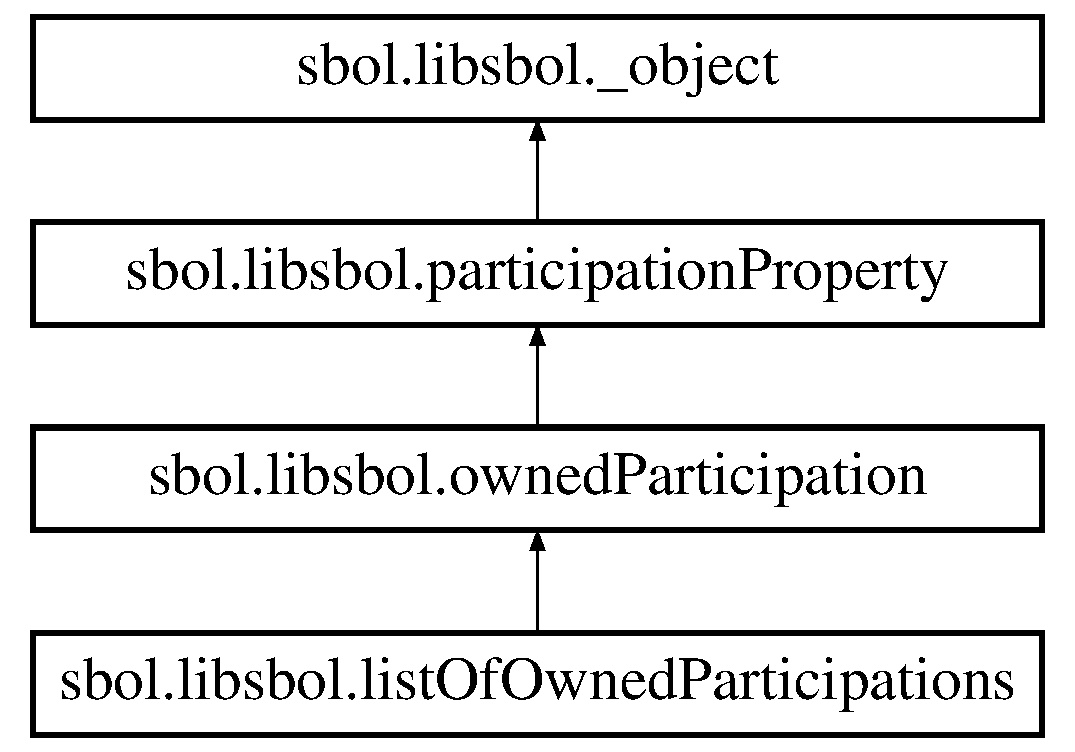
\includegraphics[height=4.000000cm]{classsbol_1_1libsbol_1_1owned_participation}
\end{center}
\end{figure}
\subsection*{Public Member Functions}
\begin{DoxyCompactItemize}
\item 
def \hyperlink{classsbol_1_1libsbol_1_1owned_participation_a616ba66360d302af0f1b85a11b97661a}{\+\_\+\+\_\+init\+\_\+\+\_\+} (self, args)
\item 
def \hyperlink{classsbol_1_1libsbol_1_1owned_participation_a214bf32aec1cbf335fb20f91a6adda06}{add} (self, sbol\+\_\+obj)
\item 
def \hyperlink{classsbol_1_1libsbol_1_1owned_participation_a476c5981a067d1d8b34ba839351e0255}{set} (self, sbol\+\_\+obj)
\item 
def \hyperlink{classsbol_1_1libsbol_1_1owned_participation_a23b698de8ba621159ca696a75b9cfc0e}{get} (self, object\+\_\+id)
\item 
def \hyperlink{classsbol_1_1libsbol_1_1owned_participation_a088b670f81c184f04b4053621a28c205}{copy} (self)
\item 
def \hyperlink{classsbol_1_1libsbol_1_1owned_participation_aabd32a1e7ea3367f72b73b78c5288cf8}{create} (self, args)
\item 
def \hyperlink{classsbol_1_1libsbol_1_1owned_participation_a52c75d9bb728ea0813d719b69ac8201b}{begin} (self)
\item 
def \hyperlink{classsbol_1_1libsbol_1_1owned_participation_a5e177d3572741babfe97d052b99c71f4}{end} (self)
\item 
def {\bfseries size} (self)\hypertarget{classsbol_1_1libsbol_1_1owned_participation_aa903f23cbe68cdb49a5dae36f1b56386}{}\label{classsbol_1_1libsbol_1_1owned_participation_aa903f23cbe68cdb49a5dae36f1b56386}

\item 
def {\bfseries \+\_\+\+\_\+getitem\+\_\+\+\_\+} (self, args)\hypertarget{classsbol_1_1libsbol_1_1owned_participation_adf8cceb293d814e010c48f5cb5f5ccd6}{}\label{classsbol_1_1libsbol_1_1owned_participation_adf8cceb293d814e010c48f5cb5f5ccd6}

\item 
def {\bfseries \+\_\+\+\_\+iter\+\_\+\+\_\+} (self)\hypertarget{classsbol_1_1libsbol_1_1owned_participation_a9d187d6ccecacb6cbf36687ba87f97fa}{}\label{classsbol_1_1libsbol_1_1owned_participation_a9d187d6ccecacb6cbf36687ba87f97fa}

\item 
def {\bfseries next} (self)\hypertarget{classsbol_1_1libsbol_1_1owned_participation_a0fb629a06a96d4f5e6544a205b0831ec}{}\label{classsbol_1_1libsbol_1_1owned_participation_a0fb629a06a96d4f5e6544a205b0831ec}

\item 
def {\bfseries \+\_\+\+\_\+len\+\_\+\+\_\+} (self)\hypertarget{classsbol_1_1libsbol_1_1owned_participation_a664aa8ce4ef4f8f430398587d65712b4}{}\label{classsbol_1_1libsbol_1_1owned_participation_a664aa8ce4ef4f8f430398587d65712b4}

\item 
def \hyperlink{classsbol_1_1libsbol_1_1owned_participation_ad7da2f4b17328e332e9cf1d112c61afa}{add\+Range} (self, sbol\+\_\+obj)
\item 
def \hyperlink{classsbol_1_1libsbol_1_1owned_participation_ac8f3a7529ef59b0c26453deca9853e0f}{get\+Range} (self)
\end{DoxyCompactItemize}
\subsection*{Public Attributes}
\begin{DoxyCompactItemize}
\item 
{\bfseries this}\hypertarget{classsbol_1_1libsbol_1_1owned_participation_a71ff8007d3575ca08734d922b7106e6d}{}\label{classsbol_1_1libsbol_1_1owned_participation_a71ff8007d3575ca08734d922b7106e6d}

\end{DoxyCompactItemize}
\subsection*{Static Public Attributes}
\begin{DoxyCompactItemize}
\item 
{\bfseries python\+\_\+iter} = \+\_\+swig\+\_\+property(\+\_\+libsbol.\+owned\+Participation\+\_\+python\+\_\+iter\+\_\+get, \+\_\+libsbol.\+owned\+Participation\+\_\+python\+\_\+iter\+\_\+set)\hypertarget{classsbol_1_1libsbol_1_1owned_participation_a27f0b38cb941000cb07a15ba05b7f387}{}\label{classsbol_1_1libsbol_1_1owned_participation_a27f0b38cb941000cb07a15ba05b7f387}

\end{DoxyCompactItemize}


\subsection{Constructor \& Destructor Documentation}
\index{sbol\+::libsbol\+::owned\+Participation@{sbol\+::libsbol\+::owned\+Participation}!\+\_\+\+\_\+init\+\_\+\+\_\+@{\+\_\+\+\_\+init\+\_\+\+\_\+}}
\index{\+\_\+\+\_\+init\+\_\+\+\_\+@{\+\_\+\+\_\+init\+\_\+\+\_\+}!sbol\+::libsbol\+::owned\+Participation@{sbol\+::libsbol\+::owned\+Participation}}
\subsubsection[{\texorpdfstring{\+\_\+\+\_\+init\+\_\+\+\_\+(self, args)}{__init__(self, args)}}]{\setlength{\rightskip}{0pt plus 5cm}def sbol.\+libsbol.\+owned\+Participation.\+\_\+\+\_\+init\+\_\+\+\_\+ (
\begin{DoxyParamCaption}
\item[{}]{self, }
\item[{}]{args}
\end{DoxyParamCaption}
)}\hypertarget{classsbol_1_1libsbol_1_1owned_participation_a616ba66360d302af0f1b85a11b97661a}{}\label{classsbol_1_1libsbol_1_1owned_participation_a616ba66360d302af0f1b85a11b97661a}
\begin{DoxyVerb}sbol::OwnedObject< SBOLClass >::OwnedObject(sbol_type type_uri, void
*property_owner, SBOLObject &first_object) 
\end{DoxyVerb}
 

\subsection{Member Function Documentation}
\index{sbol\+::libsbol\+::owned\+Participation@{sbol\+::libsbol\+::owned\+Participation}!add@{add}}
\index{add@{add}!sbol\+::libsbol\+::owned\+Participation@{sbol\+::libsbol\+::owned\+Participation}}
\subsubsection[{\texorpdfstring{add(self, sbol\+\_\+obj)}{add(self, sbol_obj)}}]{\setlength{\rightskip}{0pt plus 5cm}def sbol.\+libsbol.\+owned\+Participation.\+add (
\begin{DoxyParamCaption}
\item[{}]{self, }
\item[{}]{sbol\+\_\+obj}
\end{DoxyParamCaption}
)}\hypertarget{classsbol_1_1libsbol_1_1owned_participation_a214bf32aec1cbf335fb20f91a6adda06}{}\label{classsbol_1_1libsbol_1_1owned_participation_a214bf32aec1cbf335fb20f91a6adda06}
\begin{DoxyVerb}void
sbol::OwnedObject< SBOLClass >::add(SBOLClass &sbol_obj) 
\end{DoxyVerb}
 \index{sbol\+::libsbol\+::owned\+Participation@{sbol\+::libsbol\+::owned\+Participation}!add\+Range@{add\+Range}}
\index{add\+Range@{add\+Range}!sbol\+::libsbol\+::owned\+Participation@{sbol\+::libsbol\+::owned\+Participation}}
\subsubsection[{\texorpdfstring{add\+Range(self, sbol\+\_\+obj)}{addRange(self, sbol_obj)}}]{\setlength{\rightskip}{0pt plus 5cm}def sbol.\+libsbol.\+owned\+Participation.\+add\+Range (
\begin{DoxyParamCaption}
\item[{}]{self, }
\item[{}]{sbol\+\_\+obj}
\end{DoxyParamCaption}
)}\hypertarget{classsbol_1_1libsbol_1_1owned_participation_ad7da2f4b17328e332e9cf1d112c61afa}{}\label{classsbol_1_1libsbol_1_1owned_participation_ad7da2f4b17328e332e9cf1d112c61afa}
\begin{DoxyVerb}void
sbol::OwnedObject< SBOLClass >::add(SBOLClass &sbol_obj) 
\end{DoxyVerb}
 \index{sbol\+::libsbol\+::owned\+Participation@{sbol\+::libsbol\+::owned\+Participation}!begin@{begin}}
\index{begin@{begin}!sbol\+::libsbol\+::owned\+Participation@{sbol\+::libsbol\+::owned\+Participation}}
\subsubsection[{\texorpdfstring{begin(self)}{begin(self)}}]{\setlength{\rightskip}{0pt plus 5cm}def sbol.\+libsbol.\+owned\+Participation.\+begin (
\begin{DoxyParamCaption}
\item[{}]{self}
\end{DoxyParamCaption}
)}\hypertarget{classsbol_1_1libsbol_1_1owned_participation_a52c75d9bb728ea0813d719b69ac8201b}{}\label{classsbol_1_1libsbol_1_1owned_participation_a52c75d9bb728ea0813d719b69ac8201b}
\begin{DoxyVerb}iterator
sbol::OwnedObject< SBOLClass >::begin() 
\end{DoxyVerb}
 \index{sbol\+::libsbol\+::owned\+Participation@{sbol\+::libsbol\+::owned\+Participation}!copy@{copy}}
\index{copy@{copy}!sbol\+::libsbol\+::owned\+Participation@{sbol\+::libsbol\+::owned\+Participation}}
\subsubsection[{\texorpdfstring{copy(self)}{copy(self)}}]{\setlength{\rightskip}{0pt plus 5cm}def sbol.\+libsbol.\+owned\+Participation.\+copy (
\begin{DoxyParamCaption}
\item[{}]{self}
\end{DoxyParamCaption}
)}\hypertarget{classsbol_1_1libsbol_1_1owned_participation_a088b670f81c184f04b4053621a28c205}{}\label{classsbol_1_1libsbol_1_1owned_participation_a088b670f81c184f04b4053621a28c205}
\begin{DoxyVerb}std::vector<
SBOLClass * > sbol::OwnedObject< SBOLClass >::copy() 
\end{DoxyVerb}
 \index{sbol\+::libsbol\+::owned\+Participation@{sbol\+::libsbol\+::owned\+Participation}!create@{create}}
\index{create@{create}!sbol\+::libsbol\+::owned\+Participation@{sbol\+::libsbol\+::owned\+Participation}}
\subsubsection[{\texorpdfstring{create(self, args)}{create(self, args)}}]{\setlength{\rightskip}{0pt plus 5cm}def sbol.\+libsbol.\+owned\+Participation.\+create (
\begin{DoxyParamCaption}
\item[{}]{self, }
\item[{}]{args}
\end{DoxyParamCaption}
)}\hypertarget{classsbol_1_1libsbol_1_1owned_participation_aabd32a1e7ea3367f72b73b78c5288cf8}{}\label{classsbol_1_1libsbol_1_1owned_participation_aabd32a1e7ea3367f72b73b78c5288cf8}
\begin{DoxyVerb}void
sbol::OwnedObject< SBOLClass >::create(std::string uri_prefix,
std::string display_id, std::string version) 
\end{DoxyVerb}
 \index{sbol\+::libsbol\+::owned\+Participation@{sbol\+::libsbol\+::owned\+Participation}!end@{end}}
\index{end@{end}!sbol\+::libsbol\+::owned\+Participation@{sbol\+::libsbol\+::owned\+Participation}}
\subsubsection[{\texorpdfstring{end(self)}{end(self)}}]{\setlength{\rightskip}{0pt plus 5cm}def sbol.\+libsbol.\+owned\+Participation.\+end (
\begin{DoxyParamCaption}
\item[{}]{self}
\end{DoxyParamCaption}
)}\hypertarget{classsbol_1_1libsbol_1_1owned_participation_a5e177d3572741babfe97d052b99c71f4}{}\label{classsbol_1_1libsbol_1_1owned_participation_a5e177d3572741babfe97d052b99c71f4}
\begin{DoxyVerb}iterator
sbol::OwnedObject< SBOLClass >::end() 
\end{DoxyVerb}
 \index{sbol\+::libsbol\+::owned\+Participation@{sbol\+::libsbol\+::owned\+Participation}!get@{get}}
\index{get@{get}!sbol\+::libsbol\+::owned\+Participation@{sbol\+::libsbol\+::owned\+Participation}}
\subsubsection[{\texorpdfstring{get(self, object\+\_\+id)}{get(self, object_id)}}]{\setlength{\rightskip}{0pt plus 5cm}def sbol.\+libsbol.\+owned\+Participation.\+get (
\begin{DoxyParamCaption}
\item[{}]{self, }
\item[{}]{object\+\_\+id}
\end{DoxyParamCaption}
)}\hypertarget{classsbol_1_1libsbol_1_1owned_participation_a23b698de8ba621159ca696a75b9cfc0e}{}\label{classsbol_1_1libsbol_1_1owned_participation_a23b698de8ba621159ca696a75b9cfc0e}
\begin{DoxyVerb}SBOLClass &
sbol::OwnedObject< SBOLClass >::get(const std::string object_id) 
\end{DoxyVerb}
 \index{sbol\+::libsbol\+::owned\+Participation@{sbol\+::libsbol\+::owned\+Participation}!get\+Range@{get\+Range}}
\index{get\+Range@{get\+Range}!sbol\+::libsbol\+::owned\+Participation@{sbol\+::libsbol\+::owned\+Participation}}
\subsubsection[{\texorpdfstring{get\+Range(self)}{getRange(self)}}]{\setlength{\rightskip}{0pt plus 5cm}def sbol.\+libsbol.\+owned\+Participation.\+get\+Range (
\begin{DoxyParamCaption}
\item[{}]{self}
\end{DoxyParamCaption}
)}\hypertarget{classsbol_1_1libsbol_1_1owned_participation_ac8f3a7529ef59b0c26453deca9853e0f}{}\label{classsbol_1_1libsbol_1_1owned_participation_ac8f3a7529ef59b0c26453deca9853e0f}
\begin{DoxyVerb}SBOLClass &
sbol::OwnedObject< SBOLClass >::get(const std::string object_id) 
\end{DoxyVerb}
 \index{sbol\+::libsbol\+::owned\+Participation@{sbol\+::libsbol\+::owned\+Participation}!set@{set}}
\index{set@{set}!sbol\+::libsbol\+::owned\+Participation@{sbol\+::libsbol\+::owned\+Participation}}
\subsubsection[{\texorpdfstring{set(self, sbol\+\_\+obj)}{set(self, sbol_obj)}}]{\setlength{\rightskip}{0pt plus 5cm}def sbol.\+libsbol.\+owned\+Participation.\+set (
\begin{DoxyParamCaption}
\item[{}]{self, }
\item[{}]{sbol\+\_\+obj}
\end{DoxyParamCaption}
)}\hypertarget{classsbol_1_1libsbol_1_1owned_participation_a476c5981a067d1d8b34ba839351e0255}{}\label{classsbol_1_1libsbol_1_1owned_participation_a476c5981a067d1d8b34ba839351e0255}
\begin{DoxyVerb}void
sbol::OwnedObject< SBOLClass >::set(SBOLClass &sbol_obj) 
\end{DoxyVerb}
 

The documentation for this class was generated from the following file\+:\begin{DoxyCompactItemize}
\item 
libsbol.\+py\end{DoxyCompactItemize}

\hypertarget{classsbol_1_1libsbol_1_1owned_sequence_annotation}{}\section{sbol.\+libsbol.\+owned\+Sequence\+Annotation Class Reference}
\label{classsbol_1_1libsbol_1_1owned_sequence_annotation}\index{sbol.\+libsbol.\+owned\+Sequence\+Annotation@{sbol.\+libsbol.\+owned\+Sequence\+Annotation}}
Inheritance diagram for sbol.\+libsbol.\+owned\+Sequence\+Annotation\+:\begin{figure}[H]
\begin{center}
\leavevmode
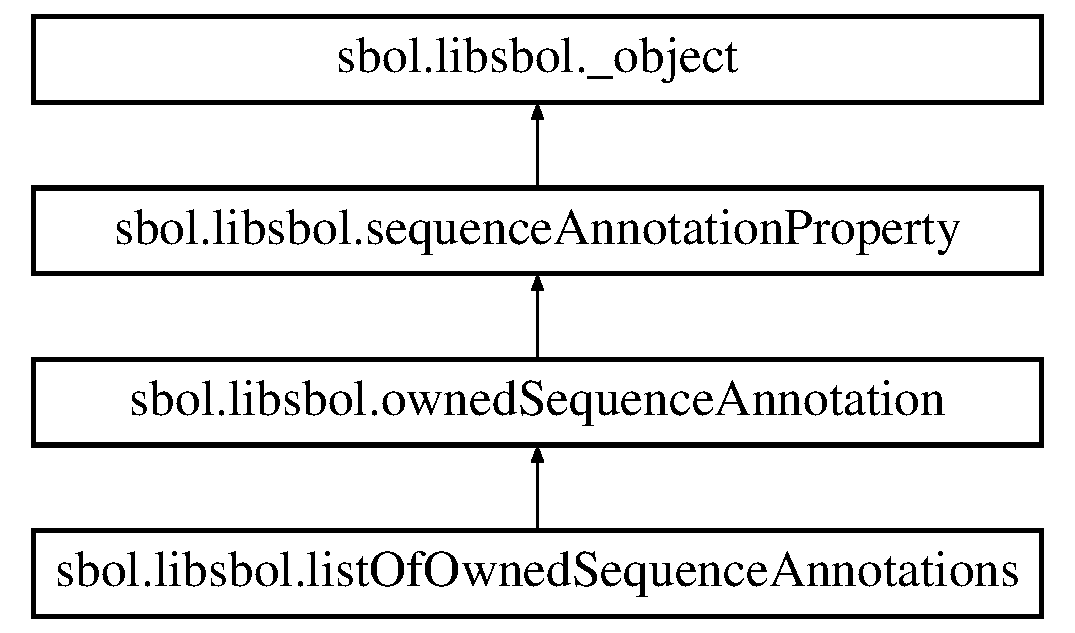
\includegraphics[height=4.000000cm]{classsbol_1_1libsbol_1_1owned_sequence_annotation}
\end{center}
\end{figure}
\subsection*{Public Member Functions}
\begin{DoxyCompactItemize}
\item 
def \hyperlink{classsbol_1_1libsbol_1_1owned_sequence_annotation_aeee3706eae9f2481ee6305b8019f774f}{\+\_\+\+\_\+init\+\_\+\+\_\+} (self, args)
\item 
def \hyperlink{classsbol_1_1libsbol_1_1owned_sequence_annotation_aa806467485d9519c52d0e419e407dd83}{add} (self, sbol\+\_\+obj)
\item 
def \hyperlink{classsbol_1_1libsbol_1_1owned_sequence_annotation_a0ff99483e3171bd1410c9a43b43a8e41}{set} (self, sbol\+\_\+obj)
\item 
def \hyperlink{classsbol_1_1libsbol_1_1owned_sequence_annotation_af053aa9e7cf71fd34ca0a15fa8d9aa84}{get} (self, object\+\_\+id)
\item 
def \hyperlink{classsbol_1_1libsbol_1_1owned_sequence_annotation_ac73169bcf0fefe7c39102a900b20b8b7}{copy} (self)
\item 
def \hyperlink{classsbol_1_1libsbol_1_1owned_sequence_annotation_ae117277e36a4da6b6f043ae7dc6ab524}{create} (self, args)
\item 
def \hyperlink{classsbol_1_1libsbol_1_1owned_sequence_annotation_af7050a8d19b361aa8903042e098daa8e}{begin} (self)
\item 
def \hyperlink{classsbol_1_1libsbol_1_1owned_sequence_annotation_a69b41606f4ae0a09785b2303888edcac}{end} (self)
\item 
def {\bfseries size} (self)\hypertarget{classsbol_1_1libsbol_1_1owned_sequence_annotation_a7b9c5d0d59ed60434eb50e576007d4ee}{}\label{classsbol_1_1libsbol_1_1owned_sequence_annotation_a7b9c5d0d59ed60434eb50e576007d4ee}

\item 
def {\bfseries \+\_\+\+\_\+getitem\+\_\+\+\_\+} (self, args)\hypertarget{classsbol_1_1libsbol_1_1owned_sequence_annotation_aa49a8d1f77e62adfab0eef439d949c1b}{}\label{classsbol_1_1libsbol_1_1owned_sequence_annotation_aa49a8d1f77e62adfab0eef439d949c1b}

\item 
def {\bfseries \+\_\+\+\_\+iter\+\_\+\+\_\+} (self)\hypertarget{classsbol_1_1libsbol_1_1owned_sequence_annotation_adb930c86ed978420759d3e0b531e5d35}{}\label{classsbol_1_1libsbol_1_1owned_sequence_annotation_adb930c86ed978420759d3e0b531e5d35}

\item 
def {\bfseries next} (self)\hypertarget{classsbol_1_1libsbol_1_1owned_sequence_annotation_a6f598e2b4013d92fe7a70135e5219d20}{}\label{classsbol_1_1libsbol_1_1owned_sequence_annotation_a6f598e2b4013d92fe7a70135e5219d20}

\item 
def {\bfseries \+\_\+\+\_\+len\+\_\+\+\_\+} (self)\hypertarget{classsbol_1_1libsbol_1_1owned_sequence_annotation_aa2532800cbd0450b9891336ad6c779e7}{}\label{classsbol_1_1libsbol_1_1owned_sequence_annotation_aa2532800cbd0450b9891336ad6c779e7}

\item 
def \hyperlink{classsbol_1_1libsbol_1_1owned_sequence_annotation_a1827114e5fecc882a6d64eb88d6696d2}{add\+Range} (self, sbol\+\_\+obj)
\item 
def \hyperlink{classsbol_1_1libsbol_1_1owned_sequence_annotation_a923a674fb3412ca07fdc5862f378b2ca}{get\+Range} (self)
\end{DoxyCompactItemize}
\subsection*{Public Attributes}
\begin{DoxyCompactItemize}
\item 
{\bfseries this}\hypertarget{classsbol_1_1libsbol_1_1owned_sequence_annotation_a100e98c00ce14984ff4e1eb5af947d5a}{}\label{classsbol_1_1libsbol_1_1owned_sequence_annotation_a100e98c00ce14984ff4e1eb5af947d5a}

\end{DoxyCompactItemize}
\subsection*{Static Public Attributes}
\begin{DoxyCompactItemize}
\item 
{\bfseries python\+\_\+iter} = \+\_\+swig\+\_\+property(\+\_\+libsbol.\+owned\+Sequence\+Annotation\+\_\+python\+\_\+iter\+\_\+get, \+\_\+libsbol.\+owned\+Sequence\+Annotation\+\_\+python\+\_\+iter\+\_\+set)\hypertarget{classsbol_1_1libsbol_1_1owned_sequence_annotation_a1fb0e40f2ed34db21f5a0736c9d49991}{}\label{classsbol_1_1libsbol_1_1owned_sequence_annotation_a1fb0e40f2ed34db21f5a0736c9d49991}

\end{DoxyCompactItemize}


\subsection{Constructor \& Destructor Documentation}
\index{sbol\+::libsbol\+::owned\+Sequence\+Annotation@{sbol\+::libsbol\+::owned\+Sequence\+Annotation}!\+\_\+\+\_\+init\+\_\+\+\_\+@{\+\_\+\+\_\+init\+\_\+\+\_\+}}
\index{\+\_\+\+\_\+init\+\_\+\+\_\+@{\+\_\+\+\_\+init\+\_\+\+\_\+}!sbol\+::libsbol\+::owned\+Sequence\+Annotation@{sbol\+::libsbol\+::owned\+Sequence\+Annotation}}
\subsubsection[{\texorpdfstring{\+\_\+\+\_\+init\+\_\+\+\_\+(self, args)}{__init__(self, args)}}]{\setlength{\rightskip}{0pt plus 5cm}def sbol.\+libsbol.\+owned\+Sequence\+Annotation.\+\_\+\+\_\+init\+\_\+\+\_\+ (
\begin{DoxyParamCaption}
\item[{}]{self, }
\item[{}]{args}
\end{DoxyParamCaption}
)}\hypertarget{classsbol_1_1libsbol_1_1owned_sequence_annotation_aeee3706eae9f2481ee6305b8019f774f}{}\label{classsbol_1_1libsbol_1_1owned_sequence_annotation_aeee3706eae9f2481ee6305b8019f774f}
\begin{DoxyVerb}sbol::OwnedObject< SBOLClass >::OwnedObject(sbol_type type_uri, void
*property_owner, SBOLObject &first_object) 
\end{DoxyVerb}
 

\subsection{Member Function Documentation}
\index{sbol\+::libsbol\+::owned\+Sequence\+Annotation@{sbol\+::libsbol\+::owned\+Sequence\+Annotation}!add@{add}}
\index{add@{add}!sbol\+::libsbol\+::owned\+Sequence\+Annotation@{sbol\+::libsbol\+::owned\+Sequence\+Annotation}}
\subsubsection[{\texorpdfstring{add(self, sbol\+\_\+obj)}{add(self, sbol_obj)}}]{\setlength{\rightskip}{0pt plus 5cm}def sbol.\+libsbol.\+owned\+Sequence\+Annotation.\+add (
\begin{DoxyParamCaption}
\item[{}]{self, }
\item[{}]{sbol\+\_\+obj}
\end{DoxyParamCaption}
)}\hypertarget{classsbol_1_1libsbol_1_1owned_sequence_annotation_aa806467485d9519c52d0e419e407dd83}{}\label{classsbol_1_1libsbol_1_1owned_sequence_annotation_aa806467485d9519c52d0e419e407dd83}
\begin{DoxyVerb}void
sbol::OwnedObject< SBOLClass >::add(SBOLClass &sbol_obj) 
\end{DoxyVerb}
 \index{sbol\+::libsbol\+::owned\+Sequence\+Annotation@{sbol\+::libsbol\+::owned\+Sequence\+Annotation}!add\+Range@{add\+Range}}
\index{add\+Range@{add\+Range}!sbol\+::libsbol\+::owned\+Sequence\+Annotation@{sbol\+::libsbol\+::owned\+Sequence\+Annotation}}
\subsubsection[{\texorpdfstring{add\+Range(self, sbol\+\_\+obj)}{addRange(self, sbol_obj)}}]{\setlength{\rightskip}{0pt plus 5cm}def sbol.\+libsbol.\+owned\+Sequence\+Annotation.\+add\+Range (
\begin{DoxyParamCaption}
\item[{}]{self, }
\item[{}]{sbol\+\_\+obj}
\end{DoxyParamCaption}
)}\hypertarget{classsbol_1_1libsbol_1_1owned_sequence_annotation_a1827114e5fecc882a6d64eb88d6696d2}{}\label{classsbol_1_1libsbol_1_1owned_sequence_annotation_a1827114e5fecc882a6d64eb88d6696d2}
\begin{DoxyVerb}void
sbol::OwnedObject< SBOLClass >::add(SBOLClass &sbol_obj) 
\end{DoxyVerb}
 \index{sbol\+::libsbol\+::owned\+Sequence\+Annotation@{sbol\+::libsbol\+::owned\+Sequence\+Annotation}!begin@{begin}}
\index{begin@{begin}!sbol\+::libsbol\+::owned\+Sequence\+Annotation@{sbol\+::libsbol\+::owned\+Sequence\+Annotation}}
\subsubsection[{\texorpdfstring{begin(self)}{begin(self)}}]{\setlength{\rightskip}{0pt plus 5cm}def sbol.\+libsbol.\+owned\+Sequence\+Annotation.\+begin (
\begin{DoxyParamCaption}
\item[{}]{self}
\end{DoxyParamCaption}
)}\hypertarget{classsbol_1_1libsbol_1_1owned_sequence_annotation_af7050a8d19b361aa8903042e098daa8e}{}\label{classsbol_1_1libsbol_1_1owned_sequence_annotation_af7050a8d19b361aa8903042e098daa8e}
\begin{DoxyVerb}iterator
sbol::OwnedObject< SBOLClass >::begin() 
\end{DoxyVerb}
 \index{sbol\+::libsbol\+::owned\+Sequence\+Annotation@{sbol\+::libsbol\+::owned\+Sequence\+Annotation}!copy@{copy}}
\index{copy@{copy}!sbol\+::libsbol\+::owned\+Sequence\+Annotation@{sbol\+::libsbol\+::owned\+Sequence\+Annotation}}
\subsubsection[{\texorpdfstring{copy(self)}{copy(self)}}]{\setlength{\rightskip}{0pt plus 5cm}def sbol.\+libsbol.\+owned\+Sequence\+Annotation.\+copy (
\begin{DoxyParamCaption}
\item[{}]{self}
\end{DoxyParamCaption}
)}\hypertarget{classsbol_1_1libsbol_1_1owned_sequence_annotation_ac73169bcf0fefe7c39102a900b20b8b7}{}\label{classsbol_1_1libsbol_1_1owned_sequence_annotation_ac73169bcf0fefe7c39102a900b20b8b7}
\begin{DoxyVerb}std::vector<
SBOLClass * > sbol::OwnedObject< SBOLClass >::copy() 
\end{DoxyVerb}
 \index{sbol\+::libsbol\+::owned\+Sequence\+Annotation@{sbol\+::libsbol\+::owned\+Sequence\+Annotation}!create@{create}}
\index{create@{create}!sbol\+::libsbol\+::owned\+Sequence\+Annotation@{sbol\+::libsbol\+::owned\+Sequence\+Annotation}}
\subsubsection[{\texorpdfstring{create(self, args)}{create(self, args)}}]{\setlength{\rightskip}{0pt plus 5cm}def sbol.\+libsbol.\+owned\+Sequence\+Annotation.\+create (
\begin{DoxyParamCaption}
\item[{}]{self, }
\item[{}]{args}
\end{DoxyParamCaption}
)}\hypertarget{classsbol_1_1libsbol_1_1owned_sequence_annotation_ae117277e36a4da6b6f043ae7dc6ab524}{}\label{classsbol_1_1libsbol_1_1owned_sequence_annotation_ae117277e36a4da6b6f043ae7dc6ab524}
\begin{DoxyVerb}void
sbol::OwnedObject< SBOLClass >::create(std::string uri_prefix,
std::string display_id, std::string version) 
\end{DoxyVerb}
 \index{sbol\+::libsbol\+::owned\+Sequence\+Annotation@{sbol\+::libsbol\+::owned\+Sequence\+Annotation}!end@{end}}
\index{end@{end}!sbol\+::libsbol\+::owned\+Sequence\+Annotation@{sbol\+::libsbol\+::owned\+Sequence\+Annotation}}
\subsubsection[{\texorpdfstring{end(self)}{end(self)}}]{\setlength{\rightskip}{0pt plus 5cm}def sbol.\+libsbol.\+owned\+Sequence\+Annotation.\+end (
\begin{DoxyParamCaption}
\item[{}]{self}
\end{DoxyParamCaption}
)}\hypertarget{classsbol_1_1libsbol_1_1owned_sequence_annotation_a69b41606f4ae0a09785b2303888edcac}{}\label{classsbol_1_1libsbol_1_1owned_sequence_annotation_a69b41606f4ae0a09785b2303888edcac}
\begin{DoxyVerb}iterator
sbol::OwnedObject< SBOLClass >::end() 
\end{DoxyVerb}
 \index{sbol\+::libsbol\+::owned\+Sequence\+Annotation@{sbol\+::libsbol\+::owned\+Sequence\+Annotation}!get@{get}}
\index{get@{get}!sbol\+::libsbol\+::owned\+Sequence\+Annotation@{sbol\+::libsbol\+::owned\+Sequence\+Annotation}}
\subsubsection[{\texorpdfstring{get(self, object\+\_\+id)}{get(self, object_id)}}]{\setlength{\rightskip}{0pt plus 5cm}def sbol.\+libsbol.\+owned\+Sequence\+Annotation.\+get (
\begin{DoxyParamCaption}
\item[{}]{self, }
\item[{}]{object\+\_\+id}
\end{DoxyParamCaption}
)}\hypertarget{classsbol_1_1libsbol_1_1owned_sequence_annotation_af053aa9e7cf71fd34ca0a15fa8d9aa84}{}\label{classsbol_1_1libsbol_1_1owned_sequence_annotation_af053aa9e7cf71fd34ca0a15fa8d9aa84}
\begin{DoxyVerb}SBOLClass &
sbol::OwnedObject< SBOLClass >::get(const std::string object_id) 
\end{DoxyVerb}
 \index{sbol\+::libsbol\+::owned\+Sequence\+Annotation@{sbol\+::libsbol\+::owned\+Sequence\+Annotation}!get\+Range@{get\+Range}}
\index{get\+Range@{get\+Range}!sbol\+::libsbol\+::owned\+Sequence\+Annotation@{sbol\+::libsbol\+::owned\+Sequence\+Annotation}}
\subsubsection[{\texorpdfstring{get\+Range(self)}{getRange(self)}}]{\setlength{\rightskip}{0pt plus 5cm}def sbol.\+libsbol.\+owned\+Sequence\+Annotation.\+get\+Range (
\begin{DoxyParamCaption}
\item[{}]{self}
\end{DoxyParamCaption}
)}\hypertarget{classsbol_1_1libsbol_1_1owned_sequence_annotation_a923a674fb3412ca07fdc5862f378b2ca}{}\label{classsbol_1_1libsbol_1_1owned_sequence_annotation_a923a674fb3412ca07fdc5862f378b2ca}
\begin{DoxyVerb}SBOLClass &
sbol::OwnedObject< SBOLClass >::get(const std::string object_id) 
\end{DoxyVerb}
 \index{sbol\+::libsbol\+::owned\+Sequence\+Annotation@{sbol\+::libsbol\+::owned\+Sequence\+Annotation}!set@{set}}
\index{set@{set}!sbol\+::libsbol\+::owned\+Sequence\+Annotation@{sbol\+::libsbol\+::owned\+Sequence\+Annotation}}
\subsubsection[{\texorpdfstring{set(self, sbol\+\_\+obj)}{set(self, sbol_obj)}}]{\setlength{\rightskip}{0pt plus 5cm}def sbol.\+libsbol.\+owned\+Sequence\+Annotation.\+set (
\begin{DoxyParamCaption}
\item[{}]{self, }
\item[{}]{sbol\+\_\+obj}
\end{DoxyParamCaption}
)}\hypertarget{classsbol_1_1libsbol_1_1owned_sequence_annotation_a0ff99483e3171bd1410c9a43b43a8e41}{}\label{classsbol_1_1libsbol_1_1owned_sequence_annotation_a0ff99483e3171bd1410c9a43b43a8e41}
\begin{DoxyVerb}void
sbol::OwnedObject< SBOLClass >::set(SBOLClass &sbol_obj) 
\end{DoxyVerb}
 

The documentation for this class was generated from the following file\+:\begin{DoxyCompactItemize}
\item 
libsbol.\+py\end{DoxyCompactItemize}

\hypertarget{classsbol_1_1libsbol_1_1owned_sequence_constraint}{}\section{sbol.\+libsbol.\+owned\+Sequence\+Constraint Class Reference}
\label{classsbol_1_1libsbol_1_1owned_sequence_constraint}\index{sbol.\+libsbol.\+owned\+Sequence\+Constraint@{sbol.\+libsbol.\+owned\+Sequence\+Constraint}}
Inheritance diagram for sbol.\+libsbol.\+owned\+Sequence\+Constraint\+:\begin{figure}[H]
\begin{center}
\leavevmode
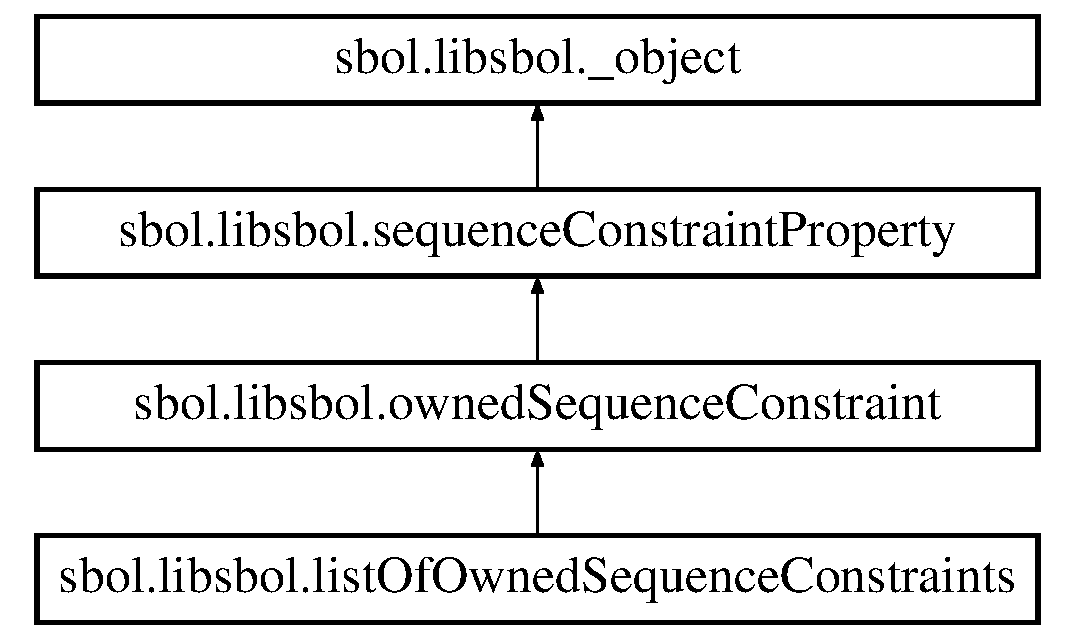
\includegraphics[height=4.000000cm]{classsbol_1_1libsbol_1_1owned_sequence_constraint}
\end{center}
\end{figure}
\subsection*{Public Member Functions}
\begin{DoxyCompactItemize}
\item 
def \hyperlink{classsbol_1_1libsbol_1_1owned_sequence_constraint_a469f435f012649d6ff695004095c7583}{\+\_\+\+\_\+init\+\_\+\+\_\+} (self, args)
\item 
def \hyperlink{classsbol_1_1libsbol_1_1owned_sequence_constraint_a7af164e6e8091380cb2740787dfd6123}{add} (self, sbol\+\_\+obj)
\item 
def \hyperlink{classsbol_1_1libsbol_1_1owned_sequence_constraint_acbfea20b113e73840128bfc242f615b9}{set} (self, sbol\+\_\+obj)
\item 
def \hyperlink{classsbol_1_1libsbol_1_1owned_sequence_constraint_abc17f99fb5d37d059762dd5a4bf29a29}{get} (self, object\+\_\+id)
\item 
def \hyperlink{classsbol_1_1libsbol_1_1owned_sequence_constraint_a709925f66902fe660c894375d8bcbb7b}{copy} (self)
\item 
def \hyperlink{classsbol_1_1libsbol_1_1owned_sequence_constraint_abcdf008085fc170ca6e35e32f182b879}{create} (self, args)
\item 
def \hyperlink{classsbol_1_1libsbol_1_1owned_sequence_constraint_a3c278bab09c98156b30c52dd31537264}{begin} (self)
\item 
def \hyperlink{classsbol_1_1libsbol_1_1owned_sequence_constraint_a1ae942f0b33f4daf1f75b59451298d69}{end} (self)
\item 
def {\bfseries size} (self)\hypertarget{classsbol_1_1libsbol_1_1owned_sequence_constraint_a51a379d2c6d60871f06e24af8f723106}{}\label{classsbol_1_1libsbol_1_1owned_sequence_constraint_a51a379d2c6d60871f06e24af8f723106}

\item 
def {\bfseries \+\_\+\+\_\+getitem\+\_\+\+\_\+} (self, args)\hypertarget{classsbol_1_1libsbol_1_1owned_sequence_constraint_ac5681a708d0dca46984fae52f88c73dd}{}\label{classsbol_1_1libsbol_1_1owned_sequence_constraint_ac5681a708d0dca46984fae52f88c73dd}

\item 
def {\bfseries \+\_\+\+\_\+iter\+\_\+\+\_\+} (self)\hypertarget{classsbol_1_1libsbol_1_1owned_sequence_constraint_a9899d67b96bc2feec34e395515e407ea}{}\label{classsbol_1_1libsbol_1_1owned_sequence_constraint_a9899d67b96bc2feec34e395515e407ea}

\item 
def {\bfseries next} (self)\hypertarget{classsbol_1_1libsbol_1_1owned_sequence_constraint_abd62d8461438354b2a5863873896c890}{}\label{classsbol_1_1libsbol_1_1owned_sequence_constraint_abd62d8461438354b2a5863873896c890}

\item 
def {\bfseries \+\_\+\+\_\+len\+\_\+\+\_\+} (self)\hypertarget{classsbol_1_1libsbol_1_1owned_sequence_constraint_ab95a9acf42cb595990084242dea5c4c2}{}\label{classsbol_1_1libsbol_1_1owned_sequence_constraint_ab95a9acf42cb595990084242dea5c4c2}

\item 
def \hyperlink{classsbol_1_1libsbol_1_1owned_sequence_constraint_a7990b1970ddccf22c40b341010238c4d}{add\+Range} (self, sbol\+\_\+obj)
\item 
def \hyperlink{classsbol_1_1libsbol_1_1owned_sequence_constraint_a665771f78c7eeb342c76eaf4dc7e2050}{get\+Range} (self)
\end{DoxyCompactItemize}
\subsection*{Public Attributes}
\begin{DoxyCompactItemize}
\item 
{\bfseries this}\hypertarget{classsbol_1_1libsbol_1_1owned_sequence_constraint_a3cc70789ae4b0c0bd261061ef94c41a3}{}\label{classsbol_1_1libsbol_1_1owned_sequence_constraint_a3cc70789ae4b0c0bd261061ef94c41a3}

\end{DoxyCompactItemize}
\subsection*{Static Public Attributes}
\begin{DoxyCompactItemize}
\item 
{\bfseries python\+\_\+iter} = \+\_\+swig\+\_\+property(\+\_\+libsbol.\+owned\+Sequence\+Constraint\+\_\+python\+\_\+iter\+\_\+get, \+\_\+libsbol.\+owned\+Sequence\+Constraint\+\_\+python\+\_\+iter\+\_\+set)\hypertarget{classsbol_1_1libsbol_1_1owned_sequence_constraint_ab1b3ee96a2594cfd1f74af6cd5d8e78f}{}\label{classsbol_1_1libsbol_1_1owned_sequence_constraint_ab1b3ee96a2594cfd1f74af6cd5d8e78f}

\end{DoxyCompactItemize}


\subsection{Constructor \& Destructor Documentation}
\index{sbol\+::libsbol\+::owned\+Sequence\+Constraint@{sbol\+::libsbol\+::owned\+Sequence\+Constraint}!\+\_\+\+\_\+init\+\_\+\+\_\+@{\+\_\+\+\_\+init\+\_\+\+\_\+}}
\index{\+\_\+\+\_\+init\+\_\+\+\_\+@{\+\_\+\+\_\+init\+\_\+\+\_\+}!sbol\+::libsbol\+::owned\+Sequence\+Constraint@{sbol\+::libsbol\+::owned\+Sequence\+Constraint}}
\subsubsection[{\texorpdfstring{\+\_\+\+\_\+init\+\_\+\+\_\+(self, args)}{__init__(self, args)}}]{\setlength{\rightskip}{0pt plus 5cm}def sbol.\+libsbol.\+owned\+Sequence\+Constraint.\+\_\+\+\_\+init\+\_\+\+\_\+ (
\begin{DoxyParamCaption}
\item[{}]{self, }
\item[{}]{args}
\end{DoxyParamCaption}
)}\hypertarget{classsbol_1_1libsbol_1_1owned_sequence_constraint_a469f435f012649d6ff695004095c7583}{}\label{classsbol_1_1libsbol_1_1owned_sequence_constraint_a469f435f012649d6ff695004095c7583}
\begin{DoxyVerb}sbol::OwnedObject< SBOLClass >::OwnedObject(sbol_type type_uri, void
*property_owner, SBOLObject &first_object) 
\end{DoxyVerb}
 

\subsection{Member Function Documentation}
\index{sbol\+::libsbol\+::owned\+Sequence\+Constraint@{sbol\+::libsbol\+::owned\+Sequence\+Constraint}!add@{add}}
\index{add@{add}!sbol\+::libsbol\+::owned\+Sequence\+Constraint@{sbol\+::libsbol\+::owned\+Sequence\+Constraint}}
\subsubsection[{\texorpdfstring{add(self, sbol\+\_\+obj)}{add(self, sbol_obj)}}]{\setlength{\rightskip}{0pt plus 5cm}def sbol.\+libsbol.\+owned\+Sequence\+Constraint.\+add (
\begin{DoxyParamCaption}
\item[{}]{self, }
\item[{}]{sbol\+\_\+obj}
\end{DoxyParamCaption}
)}\hypertarget{classsbol_1_1libsbol_1_1owned_sequence_constraint_a7af164e6e8091380cb2740787dfd6123}{}\label{classsbol_1_1libsbol_1_1owned_sequence_constraint_a7af164e6e8091380cb2740787dfd6123}
\begin{DoxyVerb}void
sbol::OwnedObject< SBOLClass >::add(SBOLClass &sbol_obj) 
\end{DoxyVerb}
 \index{sbol\+::libsbol\+::owned\+Sequence\+Constraint@{sbol\+::libsbol\+::owned\+Sequence\+Constraint}!add\+Range@{add\+Range}}
\index{add\+Range@{add\+Range}!sbol\+::libsbol\+::owned\+Sequence\+Constraint@{sbol\+::libsbol\+::owned\+Sequence\+Constraint}}
\subsubsection[{\texorpdfstring{add\+Range(self, sbol\+\_\+obj)}{addRange(self, sbol_obj)}}]{\setlength{\rightskip}{0pt plus 5cm}def sbol.\+libsbol.\+owned\+Sequence\+Constraint.\+add\+Range (
\begin{DoxyParamCaption}
\item[{}]{self, }
\item[{}]{sbol\+\_\+obj}
\end{DoxyParamCaption}
)}\hypertarget{classsbol_1_1libsbol_1_1owned_sequence_constraint_a7990b1970ddccf22c40b341010238c4d}{}\label{classsbol_1_1libsbol_1_1owned_sequence_constraint_a7990b1970ddccf22c40b341010238c4d}
\begin{DoxyVerb}void
sbol::OwnedObject< SBOLClass >::add(SBOLClass &sbol_obj) 
\end{DoxyVerb}
 \index{sbol\+::libsbol\+::owned\+Sequence\+Constraint@{sbol\+::libsbol\+::owned\+Sequence\+Constraint}!begin@{begin}}
\index{begin@{begin}!sbol\+::libsbol\+::owned\+Sequence\+Constraint@{sbol\+::libsbol\+::owned\+Sequence\+Constraint}}
\subsubsection[{\texorpdfstring{begin(self)}{begin(self)}}]{\setlength{\rightskip}{0pt plus 5cm}def sbol.\+libsbol.\+owned\+Sequence\+Constraint.\+begin (
\begin{DoxyParamCaption}
\item[{}]{self}
\end{DoxyParamCaption}
)}\hypertarget{classsbol_1_1libsbol_1_1owned_sequence_constraint_a3c278bab09c98156b30c52dd31537264}{}\label{classsbol_1_1libsbol_1_1owned_sequence_constraint_a3c278bab09c98156b30c52dd31537264}
\begin{DoxyVerb}iterator
sbol::OwnedObject< SBOLClass >::begin() 
\end{DoxyVerb}
 \index{sbol\+::libsbol\+::owned\+Sequence\+Constraint@{sbol\+::libsbol\+::owned\+Sequence\+Constraint}!copy@{copy}}
\index{copy@{copy}!sbol\+::libsbol\+::owned\+Sequence\+Constraint@{sbol\+::libsbol\+::owned\+Sequence\+Constraint}}
\subsubsection[{\texorpdfstring{copy(self)}{copy(self)}}]{\setlength{\rightskip}{0pt plus 5cm}def sbol.\+libsbol.\+owned\+Sequence\+Constraint.\+copy (
\begin{DoxyParamCaption}
\item[{}]{self}
\end{DoxyParamCaption}
)}\hypertarget{classsbol_1_1libsbol_1_1owned_sequence_constraint_a709925f66902fe660c894375d8bcbb7b}{}\label{classsbol_1_1libsbol_1_1owned_sequence_constraint_a709925f66902fe660c894375d8bcbb7b}
\begin{DoxyVerb}std::vector<
SBOLClass * > sbol::OwnedObject< SBOLClass >::copy() 
\end{DoxyVerb}
 \index{sbol\+::libsbol\+::owned\+Sequence\+Constraint@{sbol\+::libsbol\+::owned\+Sequence\+Constraint}!create@{create}}
\index{create@{create}!sbol\+::libsbol\+::owned\+Sequence\+Constraint@{sbol\+::libsbol\+::owned\+Sequence\+Constraint}}
\subsubsection[{\texorpdfstring{create(self, args)}{create(self, args)}}]{\setlength{\rightskip}{0pt plus 5cm}def sbol.\+libsbol.\+owned\+Sequence\+Constraint.\+create (
\begin{DoxyParamCaption}
\item[{}]{self, }
\item[{}]{args}
\end{DoxyParamCaption}
)}\hypertarget{classsbol_1_1libsbol_1_1owned_sequence_constraint_abcdf008085fc170ca6e35e32f182b879}{}\label{classsbol_1_1libsbol_1_1owned_sequence_constraint_abcdf008085fc170ca6e35e32f182b879}
\begin{DoxyVerb}void
sbol::OwnedObject< SBOLClass >::create(std::string uri_prefix,
std::string display_id, std::string version) 
\end{DoxyVerb}
 \index{sbol\+::libsbol\+::owned\+Sequence\+Constraint@{sbol\+::libsbol\+::owned\+Sequence\+Constraint}!end@{end}}
\index{end@{end}!sbol\+::libsbol\+::owned\+Sequence\+Constraint@{sbol\+::libsbol\+::owned\+Sequence\+Constraint}}
\subsubsection[{\texorpdfstring{end(self)}{end(self)}}]{\setlength{\rightskip}{0pt plus 5cm}def sbol.\+libsbol.\+owned\+Sequence\+Constraint.\+end (
\begin{DoxyParamCaption}
\item[{}]{self}
\end{DoxyParamCaption}
)}\hypertarget{classsbol_1_1libsbol_1_1owned_sequence_constraint_a1ae942f0b33f4daf1f75b59451298d69}{}\label{classsbol_1_1libsbol_1_1owned_sequence_constraint_a1ae942f0b33f4daf1f75b59451298d69}
\begin{DoxyVerb}iterator
sbol::OwnedObject< SBOLClass >::end() 
\end{DoxyVerb}
 \index{sbol\+::libsbol\+::owned\+Sequence\+Constraint@{sbol\+::libsbol\+::owned\+Sequence\+Constraint}!get@{get}}
\index{get@{get}!sbol\+::libsbol\+::owned\+Sequence\+Constraint@{sbol\+::libsbol\+::owned\+Sequence\+Constraint}}
\subsubsection[{\texorpdfstring{get(self, object\+\_\+id)}{get(self, object_id)}}]{\setlength{\rightskip}{0pt plus 5cm}def sbol.\+libsbol.\+owned\+Sequence\+Constraint.\+get (
\begin{DoxyParamCaption}
\item[{}]{self, }
\item[{}]{object\+\_\+id}
\end{DoxyParamCaption}
)}\hypertarget{classsbol_1_1libsbol_1_1owned_sequence_constraint_abc17f99fb5d37d059762dd5a4bf29a29}{}\label{classsbol_1_1libsbol_1_1owned_sequence_constraint_abc17f99fb5d37d059762dd5a4bf29a29}
\begin{DoxyVerb}SBOLClass &
sbol::OwnedObject< SBOLClass >::get(const std::string object_id) 
\end{DoxyVerb}
 \index{sbol\+::libsbol\+::owned\+Sequence\+Constraint@{sbol\+::libsbol\+::owned\+Sequence\+Constraint}!get\+Range@{get\+Range}}
\index{get\+Range@{get\+Range}!sbol\+::libsbol\+::owned\+Sequence\+Constraint@{sbol\+::libsbol\+::owned\+Sequence\+Constraint}}
\subsubsection[{\texorpdfstring{get\+Range(self)}{getRange(self)}}]{\setlength{\rightskip}{0pt plus 5cm}def sbol.\+libsbol.\+owned\+Sequence\+Constraint.\+get\+Range (
\begin{DoxyParamCaption}
\item[{}]{self}
\end{DoxyParamCaption}
)}\hypertarget{classsbol_1_1libsbol_1_1owned_sequence_constraint_a665771f78c7eeb342c76eaf4dc7e2050}{}\label{classsbol_1_1libsbol_1_1owned_sequence_constraint_a665771f78c7eeb342c76eaf4dc7e2050}
\begin{DoxyVerb}SBOLClass &
sbol::OwnedObject< SBOLClass >::get(const std::string object_id) 
\end{DoxyVerb}
 \index{sbol\+::libsbol\+::owned\+Sequence\+Constraint@{sbol\+::libsbol\+::owned\+Sequence\+Constraint}!set@{set}}
\index{set@{set}!sbol\+::libsbol\+::owned\+Sequence\+Constraint@{sbol\+::libsbol\+::owned\+Sequence\+Constraint}}
\subsubsection[{\texorpdfstring{set(self, sbol\+\_\+obj)}{set(self, sbol_obj)}}]{\setlength{\rightskip}{0pt plus 5cm}def sbol.\+libsbol.\+owned\+Sequence\+Constraint.\+set (
\begin{DoxyParamCaption}
\item[{}]{self, }
\item[{}]{sbol\+\_\+obj}
\end{DoxyParamCaption}
)}\hypertarget{classsbol_1_1libsbol_1_1owned_sequence_constraint_acbfea20b113e73840128bfc242f615b9}{}\label{classsbol_1_1libsbol_1_1owned_sequence_constraint_acbfea20b113e73840128bfc242f615b9}
\begin{DoxyVerb}void
sbol::OwnedObject< SBOLClass >::set(SBOLClass &sbol_obj) 
\end{DoxyVerb}
 

The documentation for this class was generated from the following file\+:\begin{DoxyCompactItemize}
\item 
libsbol.\+py\end{DoxyCompactItemize}

\hypertarget{classsbol_1_1libsbol_1_1_participation}{}\section{sbol.\+libsbol.\+Participation Class Reference}
\label{classsbol_1_1libsbol_1_1_participation}\index{sbol.\+libsbol.\+Participation@{sbol.\+libsbol.\+Participation}}
Inheritance diagram for sbol.\+libsbol.\+Participation\+:\begin{figure}[H]
\begin{center}
\leavevmode
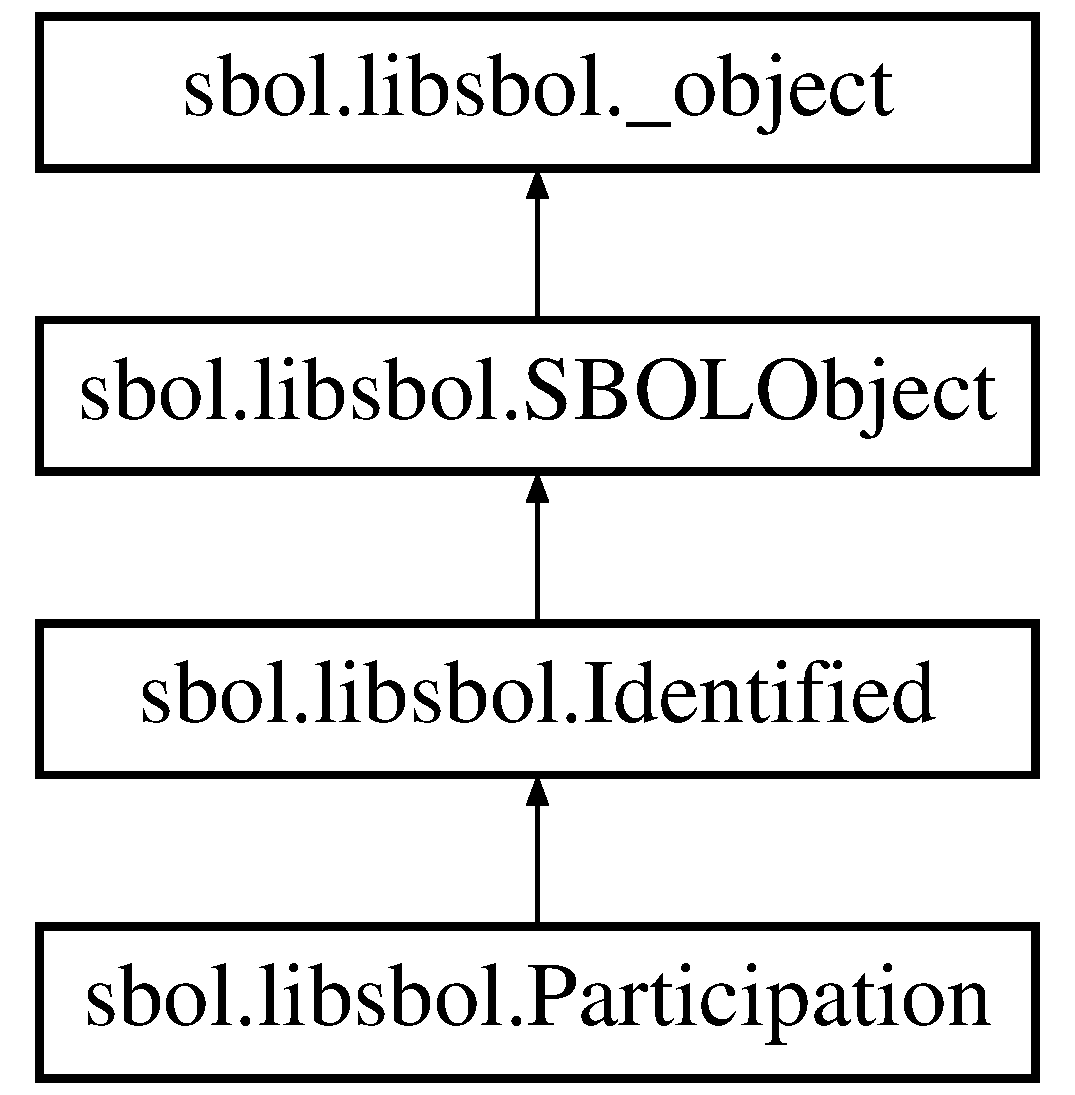
\includegraphics[height=4.000000cm]{classsbol_1_1libsbol_1_1_participation}
\end{center}
\end{figure}
\subsection*{Public Member Functions}
\begin{DoxyCompactItemize}
\item 
def \hyperlink{classsbol_1_1libsbol_1_1_participation_abdb12b708c0c470e3760031e8460f98c}{\+\_\+\+\_\+init\+\_\+\+\_\+} (self, args)
\end{DoxyCompactItemize}
\subsection*{Public Attributes}
\begin{DoxyCompactItemize}
\item 
{\bfseries this}\hypertarget{classsbol_1_1libsbol_1_1_participation_abd41f30220d0a771db4db0a9c0e74294}{}\label{classsbol_1_1libsbol_1_1_participation_abd41f30220d0a771db4db0a9c0e74294}

\end{DoxyCompactItemize}
\subsection*{Static Public Attributes}
\begin{DoxyCompactItemize}
\item 
{\bfseries roles} = \+\_\+swig\+\_\+property(\+\_\+libsbol.\+Participation\+\_\+roles\+\_\+get, \+\_\+libsbol.\+Participation\+\_\+roles\+\_\+set)\hypertarget{classsbol_1_1libsbol_1_1_participation_a3cd777ef765683dbad82e3433b6dd961}{}\label{classsbol_1_1libsbol_1_1_participation_a3cd777ef765683dbad82e3433b6dd961}

\item 
{\bfseries participant} = \+\_\+swig\+\_\+property(\+\_\+libsbol.\+Participation\+\_\+participant\+\_\+get, \+\_\+libsbol.\+Participation\+\_\+participant\+\_\+set)\hypertarget{classsbol_1_1libsbol_1_1_participation_a027d729a5d492411d90ff441b4ab18d9}{}\label{classsbol_1_1libsbol_1_1_participation_a027d729a5d492411d90ff441b4ab18d9}

\end{DoxyCompactItemize}


\subsection{Constructor \& Destructor Documentation}
\index{sbol\+::libsbol\+::\+Participation@{sbol\+::libsbol\+::\+Participation}!\+\_\+\+\_\+init\+\_\+\+\_\+@{\+\_\+\+\_\+init\+\_\+\+\_\+}}
\index{\+\_\+\+\_\+init\+\_\+\+\_\+@{\+\_\+\+\_\+init\+\_\+\+\_\+}!sbol\+::libsbol\+::\+Participation@{sbol\+::libsbol\+::\+Participation}}
\subsubsection[{\texorpdfstring{\+\_\+\+\_\+init\+\_\+\+\_\+(self, args)}{__init__(self, args)}}]{\setlength{\rightskip}{0pt plus 5cm}def sbol.\+libsbol.\+Participation.\+\_\+\+\_\+init\+\_\+\+\_\+ (
\begin{DoxyParamCaption}
\item[{}]{self, }
\item[{}]{args}
\end{DoxyParamCaption}
)}\hypertarget{classsbol_1_1libsbol_1_1_participation_abdb12b708c0c470e3760031e8460f98c}{}\label{classsbol_1_1libsbol_1_1_participation_abdb12b708c0c470e3760031e8460f98c}
\begin{DoxyVerb}sbol::Participation::Participation(std::string uri_prefix, std::string
display_id, std::string version, std::string participant) 
\end{DoxyVerb}
 

The documentation for this class was generated from the following file\+:\begin{DoxyCompactItemize}
\item 
libsbol.\+py\end{DoxyCompactItemize}

\hypertarget{classsbol_1_1libsbol_1_1participation_property}{}\section{sbol.\+libsbol.\+participation\+Property Class Reference}
\label{classsbol_1_1libsbol_1_1participation_property}\index{sbol.\+libsbol.\+participation\+Property@{sbol.\+libsbol.\+participation\+Property}}
Inheritance diagram for sbol.\+libsbol.\+participation\+Property\+:\begin{figure}[H]
\begin{center}
\leavevmode
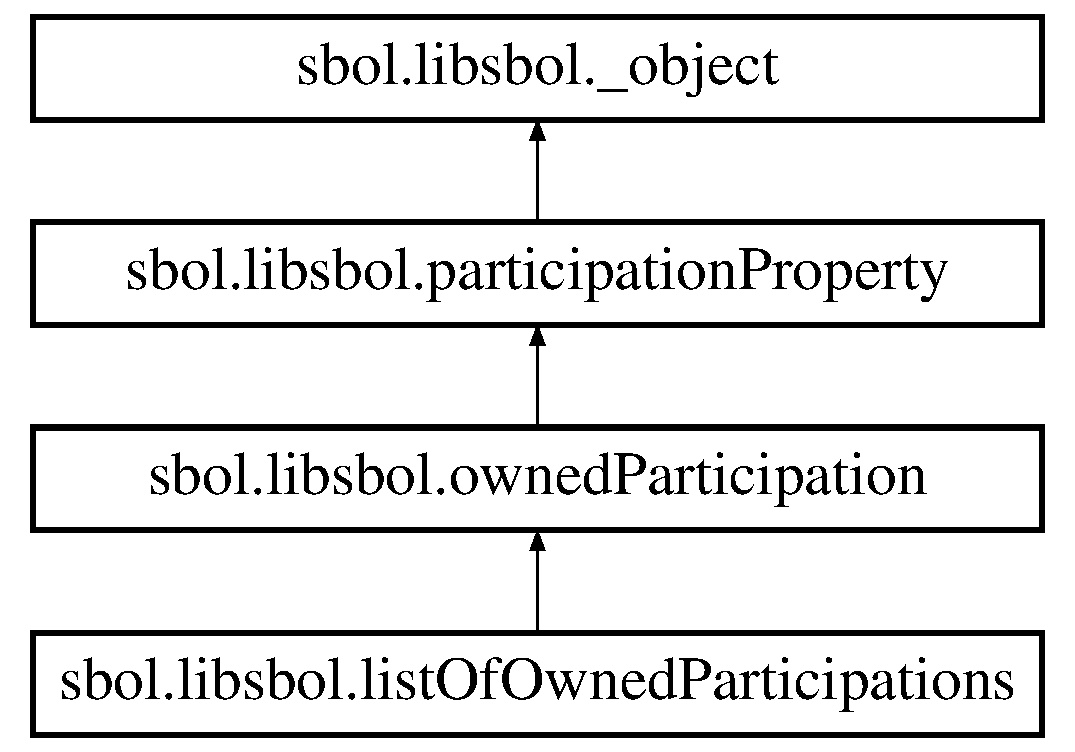
\includegraphics[height=4.000000cm]{classsbol_1_1libsbol_1_1participation_property}
\end{center}
\end{figure}
\subsection*{Public Member Functions}
\begin{DoxyCompactItemize}
\item 
def \hyperlink{classsbol_1_1libsbol_1_1participation_property_ae7279d5b838187e67021e101ea25c5f6}{\+\_\+\+\_\+init\+\_\+\+\_\+} (self, args)
\item 
def \hyperlink{classsbol_1_1libsbol_1_1participation_property_ac7cdae142635582951d2c2a7db15ec5c}{get\+Type\+U\+RI} (self)
\item 
def \hyperlink{classsbol_1_1libsbol_1_1participation_property_a0331ce40c64deaf4428b0306a1c4d879}{get\+Owner} (self)
\item 
def \hyperlink{classsbol_1_1libsbol_1_1participation_property_a0229639c831cc8da963bdc3dff7f1d51}{get} (self)
\item 
def \hyperlink{classsbol_1_1libsbol_1_1participation_property_a0154ca938cc29ad6a67d549fa599ca19}{add} (self, new\+\_\+value)
\item 
def \hyperlink{classsbol_1_1libsbol_1_1participation_property_a300280b5dbdde55100076c938ae9b6b7}{set} (self, args)
\item 
def \hyperlink{classsbol_1_1libsbol_1_1participation_property_ab8151f0316bbfe1e27f0dc8762c9bdfa}{write} (self)
\item 
def \hyperlink{classsbol_1_1libsbol_1_1participation_property_a24bf98a0ec8d680bf9ecf75e7af489a6}{validate} (self, arg=None)
\item 
def {\bfseries \+\_\+\+\_\+getitem\+\_\+\+\_\+} (self, n\+Index)\hypertarget{classsbol_1_1libsbol_1_1participation_property_ad169379204563917c452f738e5655a4a}{}\label{classsbol_1_1libsbol_1_1participation_property_ad169379204563917c452f738e5655a4a}

\item 
def {\bfseries \+\_\+\+\_\+iter\+\_\+\+\_\+} (self)\hypertarget{classsbol_1_1libsbol_1_1participation_property_a5b0fbc7d4cfd03c019a8180e97126bd8}{}\label{classsbol_1_1libsbol_1_1participation_property_a5b0fbc7d4cfd03c019a8180e97126bd8}

\item 
def {\bfseries next} (self)\hypertarget{classsbol_1_1libsbol_1_1participation_property_aa011b9f71137856a045f7e91a7201670}{}\label{classsbol_1_1libsbol_1_1participation_property_aa011b9f71137856a045f7e91a7201670}

\item 
def {\bfseries \+\_\+\+\_\+len\+\_\+\+\_\+} (self)\hypertarget{classsbol_1_1libsbol_1_1participation_property_ab54357e4b79234a4e2e78e465324b0e9}{}\label{classsbol_1_1libsbol_1_1participation_property_ab54357e4b79234a4e2e78e465324b0e9}

\end{DoxyCompactItemize}
\subsection*{Public Attributes}
\begin{DoxyCompactItemize}
\item 
{\bfseries this}\hypertarget{classsbol_1_1libsbol_1_1participation_property_aea97f91eba2637c256f5560905dff337}{}\label{classsbol_1_1libsbol_1_1participation_property_aea97f91eba2637c256f5560905dff337}

\end{DoxyCompactItemize}


\subsection{Detailed Description}
\begin{DoxyVerb}metafunction for generation of a map of message types to their
associated callbacks.

Usage: Use generate_callback_map<Type>::type to ...

Parameters:
-----------

LiteralType:  The library currently supports Property<string> and
Property<int> specification currently supports integer, string, and
URI literals

C++ includes: property.h 
\end{DoxyVerb}
 

\subsection{Constructor \& Destructor Documentation}
\index{sbol\+::libsbol\+::participation\+Property@{sbol\+::libsbol\+::participation\+Property}!\+\_\+\+\_\+init\+\_\+\+\_\+@{\+\_\+\+\_\+init\+\_\+\+\_\+}}
\index{\+\_\+\+\_\+init\+\_\+\+\_\+@{\+\_\+\+\_\+init\+\_\+\+\_\+}!sbol\+::libsbol\+::participation\+Property@{sbol\+::libsbol\+::participation\+Property}}
\subsubsection[{\texorpdfstring{\+\_\+\+\_\+init\+\_\+\+\_\+(self, args)}{__init__(self, args)}}]{\setlength{\rightskip}{0pt plus 5cm}def sbol.\+libsbol.\+participation\+Property.\+\_\+\+\_\+init\+\_\+\+\_\+ (
\begin{DoxyParamCaption}
\item[{}]{self, }
\item[{}]{args}
\end{DoxyParamCaption}
)}\hypertarget{classsbol_1_1libsbol_1_1participation_property_ae7279d5b838187e67021e101ea25c5f6}{}\label{classsbol_1_1libsbol_1_1participation_property_ae7279d5b838187e67021e101ea25c5f6}
\begin{DoxyVerb}sbol::Property<
LiteralType >::Property(sbol_type type_uri=UNDEFINED, void
*property_owner=NULL, ValidationRules validation_rules={}) 
\end{DoxyVerb}
 

\subsection{Member Function Documentation}
\index{sbol\+::libsbol\+::participation\+Property@{sbol\+::libsbol\+::participation\+Property}!add@{add}}
\index{add@{add}!sbol\+::libsbol\+::participation\+Property@{sbol\+::libsbol\+::participation\+Property}}
\subsubsection[{\texorpdfstring{add(self, new\+\_\+value)}{add(self, new_value)}}]{\setlength{\rightskip}{0pt plus 5cm}def sbol.\+libsbol.\+participation\+Property.\+add (
\begin{DoxyParamCaption}
\item[{}]{self, }
\item[{}]{new\+\_\+value}
\end{DoxyParamCaption}
)}\hypertarget{classsbol_1_1libsbol_1_1participation_property_a0154ca938cc29ad6a67d549fa599ca19}{}\label{classsbol_1_1libsbol_1_1participation_property_a0154ca938cc29ad6a67d549fa599ca19}
\begin{DoxyVerb}void sbol::Property<
LiteralType >::add(std::string new_value) 
\end{DoxyVerb}
 \index{sbol\+::libsbol\+::participation\+Property@{sbol\+::libsbol\+::participation\+Property}!get@{get}}
\index{get@{get}!sbol\+::libsbol\+::participation\+Property@{sbol\+::libsbol\+::participation\+Property}}
\subsubsection[{\texorpdfstring{get(self)}{get(self)}}]{\setlength{\rightskip}{0pt plus 5cm}def sbol.\+libsbol.\+participation\+Property.\+get (
\begin{DoxyParamCaption}
\item[{}]{self}
\end{DoxyParamCaption}
)}\hypertarget{classsbol_1_1libsbol_1_1participation_property_a0229639c831cc8da963bdc3dff7f1d51}{}\label{classsbol_1_1libsbol_1_1participation_property_a0229639c831cc8da963bdc3dff7f1d51}
\begin{DoxyVerb}std::string
sbol::Property< LiteralType >::get() 
\end{DoxyVerb}
 \index{sbol\+::libsbol\+::participation\+Property@{sbol\+::libsbol\+::participation\+Property}!get\+Owner@{get\+Owner}}
\index{get\+Owner@{get\+Owner}!sbol\+::libsbol\+::participation\+Property@{sbol\+::libsbol\+::participation\+Property}}
\subsubsection[{\texorpdfstring{get\+Owner(self)}{getOwner(self)}}]{\setlength{\rightskip}{0pt plus 5cm}def sbol.\+libsbol.\+participation\+Property.\+get\+Owner (
\begin{DoxyParamCaption}
\item[{}]{self}
\end{DoxyParamCaption}
)}\hypertarget{classsbol_1_1libsbol_1_1participation_property_a0331ce40c64deaf4428b0306a1c4d879}{}\label{classsbol_1_1libsbol_1_1participation_property_a0331ce40c64deaf4428b0306a1c4d879}
\begin{DoxyVerb}SBOLObject &
sbol::Property< LiteralType >::getOwner() 
\end{DoxyVerb}
 \index{sbol\+::libsbol\+::participation\+Property@{sbol\+::libsbol\+::participation\+Property}!get\+Type\+U\+RI@{get\+Type\+U\+RI}}
\index{get\+Type\+U\+RI@{get\+Type\+U\+RI}!sbol\+::libsbol\+::participation\+Property@{sbol\+::libsbol\+::participation\+Property}}
\subsubsection[{\texorpdfstring{get\+Type\+U\+R\+I(self)}{getTypeURI(self)}}]{\setlength{\rightskip}{0pt plus 5cm}def sbol.\+libsbol.\+participation\+Property.\+get\+Type\+U\+RI (
\begin{DoxyParamCaption}
\item[{}]{self}
\end{DoxyParamCaption}
)}\hypertarget{classsbol_1_1libsbol_1_1participation_property_ac7cdae142635582951d2c2a7db15ec5c}{}\label{classsbol_1_1libsbol_1_1participation_property_ac7cdae142635582951d2c2a7db15ec5c}
\begin{DoxyVerb}sbol_type
sbol::Property< LiteralType >::getTypeURI() 
\end{DoxyVerb}
 \index{sbol\+::libsbol\+::participation\+Property@{sbol\+::libsbol\+::participation\+Property}!set@{set}}
\index{set@{set}!sbol\+::libsbol\+::participation\+Property@{sbol\+::libsbol\+::participation\+Property}}
\subsubsection[{\texorpdfstring{set(self, args)}{set(self, args)}}]{\setlength{\rightskip}{0pt plus 5cm}def sbol.\+libsbol.\+participation\+Property.\+set (
\begin{DoxyParamCaption}
\item[{}]{self, }
\item[{}]{args}
\end{DoxyParamCaption}
)}\hypertarget{classsbol_1_1libsbol_1_1participation_property_a300280b5dbdde55100076c938ae9b6b7}{}\label{classsbol_1_1libsbol_1_1participation_property_a300280b5dbdde55100076c938ae9b6b7}
\begin{DoxyVerb}void sbol::Property<
LiteralType >::set(int new_value) 
\end{DoxyVerb}
 \index{sbol\+::libsbol\+::participation\+Property@{sbol\+::libsbol\+::participation\+Property}!validate@{validate}}
\index{validate@{validate}!sbol\+::libsbol\+::participation\+Property@{sbol\+::libsbol\+::participation\+Property}}
\subsubsection[{\texorpdfstring{validate(self, arg=\+None)}{validate(self, arg=None)}}]{\setlength{\rightskip}{0pt plus 5cm}def sbol.\+libsbol.\+participation\+Property.\+validate (
\begin{DoxyParamCaption}
\item[{}]{self, }
\item[{}]{arg = {\ttfamily None}}
\end{DoxyParamCaption}
)}\hypertarget{classsbol_1_1libsbol_1_1participation_property_a24bf98a0ec8d680bf9ecf75e7af489a6}{}\label{classsbol_1_1libsbol_1_1participation_property_a24bf98a0ec8d680bf9ecf75e7af489a6}
\begin{DoxyVerb}void sbol::Property<
LiteralType >::validate(void *arg=NULL) 
\end{DoxyVerb}
 \index{sbol\+::libsbol\+::participation\+Property@{sbol\+::libsbol\+::participation\+Property}!write@{write}}
\index{write@{write}!sbol\+::libsbol\+::participation\+Property@{sbol\+::libsbol\+::participation\+Property}}
\subsubsection[{\texorpdfstring{write(self)}{write(self)}}]{\setlength{\rightskip}{0pt plus 5cm}def sbol.\+libsbol.\+participation\+Property.\+write (
\begin{DoxyParamCaption}
\item[{}]{self}
\end{DoxyParamCaption}
)}\hypertarget{classsbol_1_1libsbol_1_1participation_property_ab8151f0316bbfe1e27f0dc8762c9bdfa}{}\label{classsbol_1_1libsbol_1_1participation_property_ab8151f0316bbfe1e27f0dc8762c9bdfa}
\begin{DoxyVerb}void sbol::Property<
LiteralType >::write() 
\end{DoxyVerb}
 

The documentation for this class was generated from the following file\+:\begin{DoxyCompactItemize}
\item 
libsbol.\+py\end{DoxyCompactItemize}

\hypertarget{classsbol_1_1libsbol_1_1_range}{}\section{sbol.\+libsbol.\+Range Class Reference}
\label{classsbol_1_1libsbol_1_1_range}\index{sbol.\+libsbol.\+Range@{sbol.\+libsbol.\+Range}}
Inheritance diagram for sbol.\+libsbol.\+Range\+:\begin{figure}[H]
\begin{center}
\leavevmode
\includegraphics[height=5.000000cm]{classsbol_1_1libsbol_1_1_range}
\end{center}
\end{figure}
\subsection*{Public Member Functions}
\begin{DoxyCompactItemize}
\item 
def \hyperlink{classsbol_1_1libsbol_1_1_range_acaca7d66f76cb30862b0ce2da7f03380}{\+\_\+\+\_\+init\+\_\+\+\_\+} (self, args)
\end{DoxyCompactItemize}
\subsection*{Public Attributes}
\begin{DoxyCompactItemize}
\item 
{\bfseries this}\hypertarget{classsbol_1_1libsbol_1_1_range_a723f677d1a9d6b83eadbfd5a8c5e4919}{}\label{classsbol_1_1libsbol_1_1_range_a723f677d1a9d6b83eadbfd5a8c5e4919}

\end{DoxyCompactItemize}
\subsection*{Static Public Attributes}
\begin{DoxyCompactItemize}
\item 
{\bfseries start} = \+\_\+swig\+\_\+property(\+\_\+libsbol.\+Range\+\_\+start\+\_\+get, \+\_\+libsbol.\+Range\+\_\+start\+\_\+set)\hypertarget{classsbol_1_1libsbol_1_1_range_aa5e49184d4560a11d40bfc7f9f3653f1}{}\label{classsbol_1_1libsbol_1_1_range_aa5e49184d4560a11d40bfc7f9f3653f1}

\item 
{\bfseries end} = \+\_\+swig\+\_\+property(\+\_\+libsbol.\+Range\+\_\+end\+\_\+get, \+\_\+libsbol.\+Range\+\_\+end\+\_\+set)\hypertarget{classsbol_1_1libsbol_1_1_range_a6d72116552669a0aaf8729a32ee5dd9c}{}\label{classsbol_1_1libsbol_1_1_range_a6d72116552669a0aaf8729a32ee5dd9c}

\end{DoxyCompactItemize}


\subsection{Constructor \& Destructor Documentation}
\index{sbol\+::libsbol\+::\+Range@{sbol\+::libsbol\+::\+Range}!\+\_\+\+\_\+init\+\_\+\+\_\+@{\+\_\+\+\_\+init\+\_\+\+\_\+}}
\index{\+\_\+\+\_\+init\+\_\+\+\_\+@{\+\_\+\+\_\+init\+\_\+\+\_\+}!sbol\+::libsbol\+::\+Range@{sbol\+::libsbol\+::\+Range}}
\subsubsection[{\texorpdfstring{\+\_\+\+\_\+init\+\_\+\+\_\+(self, args)}{__init__(self, args)}}]{\setlength{\rightskip}{0pt plus 5cm}def sbol.\+libsbol.\+Range.\+\_\+\+\_\+init\+\_\+\+\_\+ (
\begin{DoxyParamCaption}
\item[{}]{self, }
\item[{}]{args}
\end{DoxyParamCaption}
)}\hypertarget{classsbol_1_1libsbol_1_1_range_acaca7d66f76cb30862b0ce2da7f03380}{}\label{classsbol_1_1libsbol_1_1_range_acaca7d66f76cb30862b0ce2da7f03380}
\begin{DoxyVerb}sbol::Range::Range(std::string uri_prefix, std::string display_id,
std::string version, int start, int end) 
\end{DoxyVerb}
 

The documentation for this class was generated from the following file\+:\begin{DoxyCompactItemize}
\item 
libsbol.\+py\end{DoxyCompactItemize}

\hypertarget{classsbol_1_1libsbol_1_1_referenced_object}{}\section{sbol.\+libsbol.\+Referenced\+Object Class Reference}
\label{classsbol_1_1libsbol_1_1_referenced_object}\index{sbol.\+libsbol.\+Referenced\+Object@{sbol.\+libsbol.\+Referenced\+Object}}
Inheritance diagram for sbol.\+libsbol.\+Referenced\+Object\+:\begin{figure}[H]
\begin{center}
\leavevmode
\includegraphics[height=4.000000cm]{classsbol_1_1libsbol_1_1_referenced_object}
\end{center}
\end{figure}
\subsection*{Public Member Functions}
\begin{DoxyCompactItemize}
\item 
def \hyperlink{classsbol_1_1libsbol_1_1_referenced_object_a3c546c88d9b5ffd0c32d3dd85ed04e45}{\+\_\+\+\_\+init\+\_\+\+\_\+} (self, args)
\item 
def \hyperlink{classsbol_1_1libsbol_1_1_referenced_object_a10a75413cbd6ea3f0e71bb3fae7dcacf}{set} (self, uri)
\item 
def \hyperlink{classsbol_1_1libsbol_1_1_referenced_object_a2614a7188d104423a5d06acad2b94876}{add\+Reference} (self, args)
\item 
def \hyperlink{classsbol_1_1libsbol_1_1_referenced_object_aa178100da1257f783aee181906807135}{set\+Reference} (self, args)
\item 
def \hyperlink{classsbol_1_1libsbol_1_1_referenced_object_a880ec7624aa10ac445f2b17dc56f754f}{begin} (self)
\item 
def \hyperlink{classsbol_1_1libsbol_1_1_referenced_object_a28ae3ca9d96f6f037fac123a9e388294}{end} (self)
\item 
def {\bfseries size} (self)\hypertarget{classsbol_1_1libsbol_1_1_referenced_object_ac209d876022591606b808a1b448d0a75}{}\label{classsbol_1_1libsbol_1_1_referenced_object_ac209d876022591606b808a1b448d0a75}

\item 
def {\bfseries \+\_\+\+\_\+getitem\+\_\+\+\_\+} (self, n\+Index)\hypertarget{classsbol_1_1libsbol_1_1_referenced_object_a6cc74639a9ce325a148e4c5989e5cd02}{}\label{classsbol_1_1libsbol_1_1_referenced_object_a6cc74639a9ce325a148e4c5989e5cd02}

\item 
def {\bfseries \+\_\+\+\_\+iter\+\_\+\+\_\+} (self)\hypertarget{classsbol_1_1libsbol_1_1_referenced_object_aa7351b7f78664f42b84c53ac78ea19a9}{}\label{classsbol_1_1libsbol_1_1_referenced_object_aa7351b7f78664f42b84c53ac78ea19a9}

\item 
def {\bfseries next} (self)\hypertarget{classsbol_1_1libsbol_1_1_referenced_object_a119972d311062da7a8d0d2c40ec7dab8}{}\label{classsbol_1_1libsbol_1_1_referenced_object_a119972d311062da7a8d0d2c40ec7dab8}

\item 
def {\bfseries \+\_\+\+\_\+len\+\_\+\+\_\+} (self)\hypertarget{classsbol_1_1libsbol_1_1_referenced_object_a0a4a69afc4b8c619515eb0c1b87cd8ae}{}\label{classsbol_1_1libsbol_1_1_referenced_object_a0a4a69afc4b8c619515eb0c1b87cd8ae}

\end{DoxyCompactItemize}
\subsection*{Public Attributes}
\begin{DoxyCompactItemize}
\item 
{\bfseries this}\hypertarget{classsbol_1_1libsbol_1_1_referenced_object_a7c890e191effecf72931392b834ecd62}{}\label{classsbol_1_1libsbol_1_1_referenced_object_a7c890e191effecf72931392b834ecd62}

\end{DoxyCompactItemize}
\subsection*{Static Public Attributes}
\begin{DoxyCompactItemize}
\item 
{\bfseries python\+\_\+iter} = \+\_\+swig\+\_\+property(\+\_\+libsbol.\+Referenced\+Object\+\_\+python\+\_\+iter\+\_\+get, \+\_\+libsbol.\+Referenced\+Object\+\_\+python\+\_\+iter\+\_\+set)\hypertarget{classsbol_1_1libsbol_1_1_referenced_object_a3830c7a7d809e4203eff5fa50e9d4d4a}{}\label{classsbol_1_1libsbol_1_1_referenced_object_a3830c7a7d809e4203eff5fa50e9d4d4a}

\end{DoxyCompactItemize}


\subsection{Constructor \& Destructor Documentation}
\index{sbol\+::libsbol\+::\+Referenced\+Object@{sbol\+::libsbol\+::\+Referenced\+Object}!\+\_\+\+\_\+init\+\_\+\+\_\+@{\+\_\+\+\_\+init\+\_\+\+\_\+}}
\index{\+\_\+\+\_\+init\+\_\+\+\_\+@{\+\_\+\+\_\+init\+\_\+\+\_\+}!sbol\+::libsbol\+::\+Referenced\+Object@{sbol\+::libsbol\+::\+Referenced\+Object}}
\subsubsection[{\texorpdfstring{\+\_\+\+\_\+init\+\_\+\+\_\+(self, args)}{__init__(self, args)}}]{\setlength{\rightskip}{0pt plus 5cm}def sbol.\+libsbol.\+Referenced\+Object.\+\_\+\+\_\+init\+\_\+\+\_\+ (
\begin{DoxyParamCaption}
\item[{}]{self, }
\item[{}]{args}
\end{DoxyParamCaption}
)}\hypertarget{classsbol_1_1libsbol_1_1_referenced_object_a3c546c88d9b5ffd0c32d3dd85ed04e45}{}\label{classsbol_1_1libsbol_1_1_referenced_object_a3c546c88d9b5ffd0c32d3dd85ed04e45}
\begin{DoxyVerb}sbol::ReferencedObject< SBOLClass >::ReferencedObject(sbol_type
type_uri, void *property_owner, SBOLObject &first_object) 
\end{DoxyVerb}
 

\subsection{Member Function Documentation}
\index{sbol\+::libsbol\+::\+Referenced\+Object@{sbol\+::libsbol\+::\+Referenced\+Object}!add\+Reference@{add\+Reference}}
\index{add\+Reference@{add\+Reference}!sbol\+::libsbol\+::\+Referenced\+Object@{sbol\+::libsbol\+::\+Referenced\+Object}}
\subsubsection[{\texorpdfstring{add\+Reference(self, args)}{addReference(self, args)}}]{\setlength{\rightskip}{0pt plus 5cm}def sbol.\+libsbol.\+Referenced\+Object.\+add\+Reference (
\begin{DoxyParamCaption}
\item[{}]{self, }
\item[{}]{args}
\end{DoxyParamCaption}
)}\hypertarget{classsbol_1_1libsbol_1_1_referenced_object_a2614a7188d104423a5d06acad2b94876}{}\label{classsbol_1_1libsbol_1_1_referenced_object_a2614a7188d104423a5d06acad2b94876}
\begin{DoxyVerb}void
sbol::ReferencedObject< SBOLClass >::addReference(const std::string
uri_prefix, const std::string display_id, const std::string version)\end{DoxyVerb}
 \index{sbol\+::libsbol\+::\+Referenced\+Object@{sbol\+::libsbol\+::\+Referenced\+Object}!begin@{begin}}
\index{begin@{begin}!sbol\+::libsbol\+::\+Referenced\+Object@{sbol\+::libsbol\+::\+Referenced\+Object}}
\subsubsection[{\texorpdfstring{begin(self)}{begin(self)}}]{\setlength{\rightskip}{0pt plus 5cm}def sbol.\+libsbol.\+Referenced\+Object.\+begin (
\begin{DoxyParamCaption}
\item[{}]{self}
\end{DoxyParamCaption}
)}\hypertarget{classsbol_1_1libsbol_1_1_referenced_object_a880ec7624aa10ac445f2b17dc56f754f}{}\label{classsbol_1_1libsbol_1_1_referenced_object_a880ec7624aa10ac445f2b17dc56f754f}
\begin{DoxyVerb}iterator
sbol::ReferencedObject< SBOLClass >::begin() 
\end{DoxyVerb}
 \index{sbol\+::libsbol\+::\+Referenced\+Object@{sbol\+::libsbol\+::\+Referenced\+Object}!end@{end}}
\index{end@{end}!sbol\+::libsbol\+::\+Referenced\+Object@{sbol\+::libsbol\+::\+Referenced\+Object}}
\subsubsection[{\texorpdfstring{end(self)}{end(self)}}]{\setlength{\rightskip}{0pt plus 5cm}def sbol.\+libsbol.\+Referenced\+Object.\+end (
\begin{DoxyParamCaption}
\item[{}]{self}
\end{DoxyParamCaption}
)}\hypertarget{classsbol_1_1libsbol_1_1_referenced_object_a28ae3ca9d96f6f037fac123a9e388294}{}\label{classsbol_1_1libsbol_1_1_referenced_object_a28ae3ca9d96f6f037fac123a9e388294}
\begin{DoxyVerb}iterator
sbol::ReferencedObject< SBOLClass >::end() 
\end{DoxyVerb}
 \index{sbol\+::libsbol\+::\+Referenced\+Object@{sbol\+::libsbol\+::\+Referenced\+Object}!set@{set}}
\index{set@{set}!sbol\+::libsbol\+::\+Referenced\+Object@{sbol\+::libsbol\+::\+Referenced\+Object}}
\subsubsection[{\texorpdfstring{set(self, uri)}{set(self, uri)}}]{\setlength{\rightskip}{0pt plus 5cm}def sbol.\+libsbol.\+Referenced\+Object.\+set (
\begin{DoxyParamCaption}
\item[{}]{self, }
\item[{}]{uri}
\end{DoxyParamCaption}
)}\hypertarget{classsbol_1_1libsbol_1_1_referenced_object_a10a75413cbd6ea3f0e71bb3fae7dcacf}{}\label{classsbol_1_1libsbol_1_1_referenced_object_a10a75413cbd6ea3f0e71bb3fae7dcacf}
\begin{DoxyVerb}void
sbol::ReferencedObject< SBOLClass >::set(SBOLClass &sbol_obj) 
\end{DoxyVerb}
 \index{sbol\+::libsbol\+::\+Referenced\+Object@{sbol\+::libsbol\+::\+Referenced\+Object}!set\+Reference@{set\+Reference}}
\index{set\+Reference@{set\+Reference}!sbol\+::libsbol\+::\+Referenced\+Object@{sbol\+::libsbol\+::\+Referenced\+Object}}
\subsubsection[{\texorpdfstring{set\+Reference(self, args)}{setReference(self, args)}}]{\setlength{\rightskip}{0pt plus 5cm}def sbol.\+libsbol.\+Referenced\+Object.\+set\+Reference (
\begin{DoxyParamCaption}
\item[{}]{self, }
\item[{}]{args}
\end{DoxyParamCaption}
)}\hypertarget{classsbol_1_1libsbol_1_1_referenced_object_aa178100da1257f783aee181906807135}{}\label{classsbol_1_1libsbol_1_1_referenced_object_aa178100da1257f783aee181906807135}
\begin{DoxyVerb}void
sbol::ReferencedObject< SBOLClass >::setReference(const std::string
uri_prefix, const std::string display_id, const std::string version)\end{DoxyVerb}
 

The documentation for this class was generated from the following file\+:\begin{DoxyCompactItemize}
\item 
libsbol.\+py\end{DoxyCompactItemize}

\hypertarget{classsbol_1_1libsbol_1_1_s_b_o_l_object}{}\section{sbol.\+libsbol.\+S\+B\+O\+L\+Object Class Reference}
\label{classsbol_1_1libsbol_1_1_s_b_o_l_object}\index{sbol.\+libsbol.\+S\+B\+O\+L\+Object@{sbol.\+libsbol.\+S\+B\+O\+L\+Object}}
Inheritance diagram for sbol.\+libsbol.\+S\+B\+O\+L\+Object\+:\begin{figure}[H]
\begin{center}
\leavevmode
\includegraphics[height=12.000000cm]{classsbol_1_1libsbol_1_1_s_b_o_l_object}
\end{center}
\end{figure}
\subsection*{Public Member Functions}
\begin{DoxyCompactItemize}
\item 
def \hyperlink{classsbol_1_1libsbol_1_1_s_b_o_l_object_a28ad02e95f0e7cbbe3d602726c8e9f4a}{\+\_\+\+\_\+init\+\_\+\+\_\+} (self, args)
\item 
def \hyperlink{classsbol_1_1libsbol_1_1_s_b_o_l_object_a0f432bb4970ca81886d5138211889706}{get\+Type\+U\+RI} (self)
\item 
def \hyperlink{classsbol_1_1libsbol_1_1_s_b_o_l_object_a4540642f2088dfc567724b62804ca565}{serialize} (self, sbol\+\_\+serializer, sbol\+\_\+world=None)
\item 
def \hyperlink{classsbol_1_1libsbol_1_1_s_b_o_l_object_a2aa7275cf01c56b112ea9dba20fca185}{nest} (self, rdfxml\+\_\+buffer)
\item 
def \hyperlink{classsbol_1_1libsbol_1_1_s_b_o_l_object_a17bd27ccb1e0b383eff0db940ad2a18b}{get\+Class\+Name} (self, type)
\item 
def {\bfseries \+\_\+\+\_\+repr\+\_\+\+\_\+} (self)\hypertarget{classsbol_1_1libsbol_1_1_s_b_o_l_object_ade31d7264979c1f136f0c68b376760f8}{}\label{classsbol_1_1libsbol_1_1_s_b_o_l_object_ade31d7264979c1f136f0c68b376760f8}

\item 
def {\bfseries \+\_\+\+\_\+str\+\_\+\+\_\+} (self)\hypertarget{classsbol_1_1libsbol_1_1_s_b_o_l_object_a4d075956912053ac0b22700924d1fded}{}\label{classsbol_1_1libsbol_1_1_s_b_o_l_object_a4d075956912053ac0b22700924d1fded}

\end{DoxyCompactItemize}
\subsection*{Public Attributes}
\begin{DoxyCompactItemize}
\item 
{\bfseries this}\hypertarget{classsbol_1_1libsbol_1_1_s_b_o_l_object_ab6fd35f2ee439159a94765fd116ede51}{}\label{classsbol_1_1libsbol_1_1_s_b_o_l_object_ab6fd35f2ee439159a94765fd116ede51}

\end{DoxyCompactItemize}
\subsection*{Static Public Attributes}
\begin{DoxyCompactItemize}
\item 
{\bfseries doc} = \+\_\+swig\+\_\+property(\+\_\+libsbol.\+S\+B\+O\+L\+Object\+\_\+doc\+\_\+get, \+\_\+libsbol.\+S\+B\+O\+L\+Object\+\_\+doc\+\_\+set)\hypertarget{classsbol_1_1libsbol_1_1_s_b_o_l_object_a7418b65d987c1adc463a46557c4c46e5}{}\label{classsbol_1_1libsbol_1_1_s_b_o_l_object_a7418b65d987c1adc463a46557c4c46e5}

\item 
{\bfseries properties} = \+\_\+swig\+\_\+property(\+\_\+libsbol.\+S\+B\+O\+L\+Object\+\_\+properties\+\_\+get, \+\_\+libsbol.\+S\+B\+O\+L\+Object\+\_\+properties\+\_\+set)\hypertarget{classsbol_1_1libsbol_1_1_s_b_o_l_object_af01b08e5e017c7ac1411d89d2f1e50c6}{}\label{classsbol_1_1libsbol_1_1_s_b_o_l_object_af01b08e5e017c7ac1411d89d2f1e50c6}

\item 
{\bfseries list\+\_\+properties} = \+\_\+swig\+\_\+property(\+\_\+libsbol.\+S\+B\+O\+L\+Object\+\_\+list\+\_\+properties\+\_\+get, \+\_\+libsbol.\+S\+B\+O\+L\+Object\+\_\+list\+\_\+properties\+\_\+set)\hypertarget{classsbol_1_1libsbol_1_1_s_b_o_l_object_a4e87936f235fc46b948377b5af646965}{}\label{classsbol_1_1libsbol_1_1_s_b_o_l_object_a4e87936f235fc46b948377b5af646965}

\item 
{\bfseries owned\+\_\+objects} = \+\_\+swig\+\_\+property(\+\_\+libsbol.\+S\+B\+O\+L\+Object\+\_\+owned\+\_\+objects\+\_\+get, \+\_\+libsbol.\+S\+B\+O\+L\+Object\+\_\+owned\+\_\+objects\+\_\+set)\hypertarget{classsbol_1_1libsbol_1_1_s_b_o_l_object_abb757d2bee6cedc04161bd0d98ff6111}{}\label{classsbol_1_1libsbol_1_1_s_b_o_l_object_abb757d2bee6cedc04161bd0d98ff6111}

\item 
{\bfseries type} = \+\_\+swig\+\_\+property(\+\_\+libsbol.\+S\+B\+O\+L\+Object\+\_\+type\+\_\+get, \+\_\+libsbol.\+S\+B\+O\+L\+Object\+\_\+type\+\_\+set)\hypertarget{classsbol_1_1libsbol_1_1_s_b_o_l_object_a18c1b12529d576ccc2166e5673c14f52}{}\label{classsbol_1_1libsbol_1_1_s_b_o_l_object_a18c1b12529d576ccc2166e5673c14f52}

\item 
{\bfseries identity} = \+\_\+swig\+\_\+property(\+\_\+libsbol.\+S\+B\+O\+L\+Object\+\_\+identity\+\_\+get, \+\_\+libsbol.\+S\+B\+O\+L\+Object\+\_\+identity\+\_\+set)\hypertarget{classsbol_1_1libsbol_1_1_s_b_o_l_object_a19c8ed60369e5ec53e0a23b67c381d06}{}\label{classsbol_1_1libsbol_1_1_s_b_o_l_object_a19c8ed60369e5ec53e0a23b67c381d06}

\end{DoxyCompactItemize}


\subsection{Constructor \& Destructor Documentation}
\index{sbol\+::libsbol\+::\+S\+B\+O\+L\+Object@{sbol\+::libsbol\+::\+S\+B\+O\+L\+Object}!\+\_\+\+\_\+init\+\_\+\+\_\+@{\+\_\+\+\_\+init\+\_\+\+\_\+}}
\index{\+\_\+\+\_\+init\+\_\+\+\_\+@{\+\_\+\+\_\+init\+\_\+\+\_\+}!sbol\+::libsbol\+::\+S\+B\+O\+L\+Object@{sbol\+::libsbol\+::\+S\+B\+O\+L\+Object}}
\subsubsection[{\texorpdfstring{\+\_\+\+\_\+init\+\_\+\+\_\+(self, args)}{__init__(self, args)}}]{\setlength{\rightskip}{0pt plus 5cm}def sbol.\+libsbol.\+S\+B\+O\+L\+Object.\+\_\+\+\_\+init\+\_\+\+\_\+ (
\begin{DoxyParamCaption}
\item[{}]{self, }
\item[{}]{args}
\end{DoxyParamCaption}
)}\hypertarget{classsbol_1_1libsbol_1_1_s_b_o_l_object_a28ad02e95f0e7cbbe3d602726c8e9f4a}{}\label{classsbol_1_1libsbol_1_1_s_b_o_l_object_a28ad02e95f0e7cbbe3d602726c8e9f4a}
\begin{DoxyVerb}sbol::SBOLObject::SBOLObject(std::string uri_prefix, std::string
display_id, std::string version) 
\end{DoxyVerb}
 

\subsection{Member Function Documentation}
\index{sbol\+::libsbol\+::\+S\+B\+O\+L\+Object@{sbol\+::libsbol\+::\+S\+B\+O\+L\+Object}!get\+Class\+Name@{get\+Class\+Name}}
\index{get\+Class\+Name@{get\+Class\+Name}!sbol\+::libsbol\+::\+S\+B\+O\+L\+Object@{sbol\+::libsbol\+::\+S\+B\+O\+L\+Object}}
\subsubsection[{\texorpdfstring{get\+Class\+Name(self, type)}{getClassName(self, type)}}]{\setlength{\rightskip}{0pt plus 5cm}def sbol.\+libsbol.\+S\+B\+O\+L\+Object.\+get\+Class\+Name (
\begin{DoxyParamCaption}
\item[{}]{self, }
\item[{}]{type}
\end{DoxyParamCaption}
)}\hypertarget{classsbol_1_1libsbol_1_1_s_b_o_l_object_a17bd27ccb1e0b383eff0db940ad2a18b}{}\label{classsbol_1_1libsbol_1_1_s_b_o_l_object_a17bd27ccb1e0b383eff0db940ad2a18b}
\begin{DoxyVerb}std::string
sbol::SBOLObject::getClassName(std::string type) 
\end{DoxyVerb}
 \index{sbol\+::libsbol\+::\+S\+B\+O\+L\+Object@{sbol\+::libsbol\+::\+S\+B\+O\+L\+Object}!get\+Type\+U\+RI@{get\+Type\+U\+RI}}
\index{get\+Type\+U\+RI@{get\+Type\+U\+RI}!sbol\+::libsbol\+::\+S\+B\+O\+L\+Object@{sbol\+::libsbol\+::\+S\+B\+O\+L\+Object}}
\subsubsection[{\texorpdfstring{get\+Type\+U\+R\+I(self)}{getTypeURI(self)}}]{\setlength{\rightskip}{0pt plus 5cm}def sbol.\+libsbol.\+S\+B\+O\+L\+Object.\+get\+Type\+U\+RI (
\begin{DoxyParamCaption}
\item[{}]{self}
\end{DoxyParamCaption}
)}\hypertarget{classsbol_1_1libsbol_1_1_s_b_o_l_object_a0f432bb4970ca81886d5138211889706}{}\label{classsbol_1_1libsbol_1_1_s_b_o_l_object_a0f432bb4970ca81886d5138211889706}
\begin{DoxyVerb}virtual
sbol_type sbol::SBOLObject::getTypeURI() 
\end{DoxyVerb}
 \index{sbol\+::libsbol\+::\+S\+B\+O\+L\+Object@{sbol\+::libsbol\+::\+S\+B\+O\+L\+Object}!nest@{nest}}
\index{nest@{nest}!sbol\+::libsbol\+::\+S\+B\+O\+L\+Object@{sbol\+::libsbol\+::\+S\+B\+O\+L\+Object}}
\subsubsection[{\texorpdfstring{nest(self, rdfxml\+\_\+buffer)}{nest(self, rdfxml_buffer)}}]{\setlength{\rightskip}{0pt plus 5cm}def sbol.\+libsbol.\+S\+B\+O\+L\+Object.\+nest (
\begin{DoxyParamCaption}
\item[{}]{self, }
\item[{}]{rdfxml\+\_\+buffer}
\end{DoxyParamCaption}
)}\hypertarget{classsbol_1_1libsbol_1_1_s_b_o_l_object_a2aa7275cf01c56b112ea9dba20fca185}{}\label{classsbol_1_1libsbol_1_1_s_b_o_l_object_a2aa7275cf01c56b112ea9dba20fca185}
\begin{DoxyVerb}std::string
sbol::SBOLObject::nest(std::string &rdfxml_buffer) 
\end{DoxyVerb}
 \index{sbol\+::libsbol\+::\+S\+B\+O\+L\+Object@{sbol\+::libsbol\+::\+S\+B\+O\+L\+Object}!serialize@{serialize}}
\index{serialize@{serialize}!sbol\+::libsbol\+::\+S\+B\+O\+L\+Object@{sbol\+::libsbol\+::\+S\+B\+O\+L\+Object}}
\subsubsection[{\texorpdfstring{serialize(self, sbol\+\_\+serializer, sbol\+\_\+world=\+None)}{serialize(self, sbol_serializer, sbol_world=None)}}]{\setlength{\rightskip}{0pt plus 5cm}def sbol.\+libsbol.\+S\+B\+O\+L\+Object.\+serialize (
\begin{DoxyParamCaption}
\item[{}]{self, }
\item[{}]{sbol\+\_\+serializer, }
\item[{}]{sbol\+\_\+world = {\ttfamily None}}
\end{DoxyParamCaption}
)}\hypertarget{classsbol_1_1libsbol_1_1_s_b_o_l_object_a4540642f2088dfc567724b62804ca565}{}\label{classsbol_1_1libsbol_1_1_s_b_o_l_object_a4540642f2088dfc567724b62804ca565}
\begin{DoxyVerb}void
sbol::SBOLObject::serialize(raptor_serializer *sbol_serializer,
raptor_world *sbol_world=NULL) 
\end{DoxyVerb}
 

The documentation for this class was generated from the following file\+:\begin{DoxyCompactItemize}
\item 
libsbol.\+py\end{DoxyCompactItemize}

\hypertarget{classsbol_1_1libsbol_1_1_sequence}{}\section{sbol.\+libsbol.\+Sequence Class Reference}
\label{classsbol_1_1libsbol_1_1_sequence}\index{sbol.\+libsbol.\+Sequence@{sbol.\+libsbol.\+Sequence}}
Inheritance diagram for sbol.\+libsbol.\+Sequence\+:\begin{figure}[H]
\begin{center}
\leavevmode
\includegraphics[height=5.000000cm]{classsbol_1_1libsbol_1_1_sequence}
\end{center}
\end{figure}
\subsection*{Public Member Functions}
\begin{DoxyCompactItemize}
\item 
def \hyperlink{classsbol_1_1libsbol_1_1_sequence_ac6d617b37f202f81698b1e83a8e9a03e}{\+\_\+\+\_\+init\+\_\+\+\_\+} (self, args)
\end{DoxyCompactItemize}
\subsection*{Public Attributes}
\begin{DoxyCompactItemize}
\item 
{\bfseries this}\hypertarget{classsbol_1_1libsbol_1_1_sequence_aee1ca0c7cf023dc44e072f39247094a0}{}\label{classsbol_1_1libsbol_1_1_sequence_aee1ca0c7cf023dc44e072f39247094a0}

\end{DoxyCompactItemize}
\subsection*{Static Public Attributes}
\begin{DoxyCompactItemize}
\item 
{\bfseries elements} = \+\_\+swig\+\_\+property(\+\_\+libsbol.\+Sequence\+\_\+elements\+\_\+get, \+\_\+libsbol.\+Sequence\+\_\+elements\+\_\+set)\hypertarget{classsbol_1_1libsbol_1_1_sequence_a754eabfce59cef5db565e3ec3202a666}{}\label{classsbol_1_1libsbol_1_1_sequence_a754eabfce59cef5db565e3ec3202a666}

\item 
{\bfseries encoding} = \+\_\+swig\+\_\+property(\+\_\+libsbol.\+Sequence\+\_\+encoding\+\_\+get, \+\_\+libsbol.\+Sequence\+\_\+encoding\+\_\+set)\hypertarget{classsbol_1_1libsbol_1_1_sequence_ab1e7d498703948dbde7ba4c7b8405742}{}\label{classsbol_1_1libsbol_1_1_sequence_ab1e7d498703948dbde7ba4c7b8405742}

\end{DoxyCompactItemize}


\subsection{Constructor \& Destructor Documentation}
\index{sbol\+::libsbol\+::\+Sequence@{sbol\+::libsbol\+::\+Sequence}!\+\_\+\+\_\+init\+\_\+\+\_\+@{\+\_\+\+\_\+init\+\_\+\+\_\+}}
\index{\+\_\+\+\_\+init\+\_\+\+\_\+@{\+\_\+\+\_\+init\+\_\+\+\_\+}!sbol\+::libsbol\+::\+Sequence@{sbol\+::libsbol\+::\+Sequence}}
\subsubsection[{\texorpdfstring{\+\_\+\+\_\+init\+\_\+\+\_\+(self, args)}{__init__(self, args)}}]{\setlength{\rightskip}{0pt plus 5cm}def sbol.\+libsbol.\+Sequence.\+\_\+\+\_\+init\+\_\+\+\_\+ (
\begin{DoxyParamCaption}
\item[{}]{self, }
\item[{}]{args}
\end{DoxyParamCaption}
)}\hypertarget{classsbol_1_1libsbol_1_1_sequence_ac6d617b37f202f81698b1e83a8e9a03e}{}\label{classsbol_1_1libsbol_1_1_sequence_ac6d617b37f202f81698b1e83a8e9a03e}
\begin{DoxyVerb}sbol::Sequence::Sequence(std::string uri_prefix, std::string
display_id, std::string version, std::string elements, std::string
encoding) 
\end{DoxyVerb}
 

The documentation for this class was generated from the following file\+:\begin{DoxyCompactItemize}
\item 
libsbol.\+py\end{DoxyCompactItemize}

\hypertarget{classsbol_1_1libsbol_1_1_sequence_annotation}{}\section{sbol.\+libsbol.\+Sequence\+Annotation Class Reference}
\label{classsbol_1_1libsbol_1_1_sequence_annotation}\index{sbol.\+libsbol.\+Sequence\+Annotation@{sbol.\+libsbol.\+Sequence\+Annotation}}
Inheritance diagram for sbol.\+libsbol.\+Sequence\+Annotation\+:\begin{figure}[H]
\begin{center}
\leavevmode
\includegraphics[height=4.000000cm]{classsbol_1_1libsbol_1_1_sequence_annotation}
\end{center}
\end{figure}
\subsection*{Public Member Functions}
\begin{DoxyCompactItemize}
\item 
def \hyperlink{classsbol_1_1libsbol_1_1_sequence_annotation_a9db7889cd3ee1aecb49ed913557d0631}{\+\_\+\+\_\+init\+\_\+\+\_\+} (self, args)
\end{DoxyCompactItemize}
\subsection*{Public Attributes}
\begin{DoxyCompactItemize}
\item 
{\bfseries this}\hypertarget{classsbol_1_1libsbol_1_1_sequence_annotation_a3db1cb1feca5848509cee7e39cee9d4d}{}\label{classsbol_1_1libsbol_1_1_sequence_annotation_a3db1cb1feca5848509cee7e39cee9d4d}

\end{DoxyCompactItemize}
\subsection*{Static Public Attributes}
\begin{DoxyCompactItemize}
\item 
{\bfseries locations} = \+\_\+swig\+\_\+property(\+\_\+libsbol.\+Sequence\+Annotation\+\_\+locations\+\_\+get, \+\_\+libsbol.\+Sequence\+Annotation\+\_\+locations\+\_\+set)\hypertarget{classsbol_1_1libsbol_1_1_sequence_annotation_a4f4742a70a4c391f547f5ad02faeb825}{}\label{classsbol_1_1libsbol_1_1_sequence_annotation_a4f4742a70a4c391f547f5ad02faeb825}

\end{DoxyCompactItemize}


\subsection{Constructor \& Destructor Documentation}
\index{sbol\+::libsbol\+::\+Sequence\+Annotation@{sbol\+::libsbol\+::\+Sequence\+Annotation}!\+\_\+\+\_\+init\+\_\+\+\_\+@{\+\_\+\+\_\+init\+\_\+\+\_\+}}
\index{\+\_\+\+\_\+init\+\_\+\+\_\+@{\+\_\+\+\_\+init\+\_\+\+\_\+}!sbol\+::libsbol\+::\+Sequence\+Annotation@{sbol\+::libsbol\+::\+Sequence\+Annotation}}
\subsubsection[{\texorpdfstring{\+\_\+\+\_\+init\+\_\+\+\_\+(self, args)}{__init__(self, args)}}]{\setlength{\rightskip}{0pt plus 5cm}def sbol.\+libsbol.\+Sequence\+Annotation.\+\_\+\+\_\+init\+\_\+\+\_\+ (
\begin{DoxyParamCaption}
\item[{}]{self, }
\item[{}]{args}
\end{DoxyParamCaption}
)}\hypertarget{classsbol_1_1libsbol_1_1_sequence_annotation_a9db7889cd3ee1aecb49ed913557d0631}{}\label{classsbol_1_1libsbol_1_1_sequence_annotation_a9db7889cd3ee1aecb49ed913557d0631}
\begin{DoxyVerb}sbol::SequenceAnnotation::SequenceAnnotation(std::string uri_prefix,
std::string display_id, std::string version) 
\end{DoxyVerb}
 

The documentation for this class was generated from the following file\+:\begin{DoxyCompactItemize}
\item 
libsbol.\+py\end{DoxyCompactItemize}

\hypertarget{classsbol_1_1libsbol_1_1sequence_annotation_property}{}\section{sbol.\+libsbol.\+sequence\+Annotation\+Property Class Reference}
\label{classsbol_1_1libsbol_1_1sequence_annotation_property}\index{sbol.\+libsbol.\+sequence\+Annotation\+Property@{sbol.\+libsbol.\+sequence\+Annotation\+Property}}
Inheritance diagram for sbol.\+libsbol.\+sequence\+Annotation\+Property\+:\begin{figure}[H]
\begin{center}
\leavevmode
\includegraphics[height=4.000000cm]{classsbol_1_1libsbol_1_1sequence_annotation_property}
\end{center}
\end{figure}
\subsection*{Public Member Functions}
\begin{DoxyCompactItemize}
\item 
def \hyperlink{classsbol_1_1libsbol_1_1sequence_annotation_property_adbec53bde8e9b5a4aea1dcb38996e22a}{\+\_\+\+\_\+init\+\_\+\+\_\+} (self, args)
\item 
def \hyperlink{classsbol_1_1libsbol_1_1sequence_annotation_property_ab5dcce148271a007e99214b9d60718eb}{get\+Type\+U\+RI} (self)
\item 
def \hyperlink{classsbol_1_1libsbol_1_1sequence_annotation_property_a425986d06731ad6afff1f778d21e5f48}{get\+Owner} (self)
\item 
def \hyperlink{classsbol_1_1libsbol_1_1sequence_annotation_property_abd7d15f4742deffdf166894ee44b858c}{get} (self)
\item 
def \hyperlink{classsbol_1_1libsbol_1_1sequence_annotation_property_a7fd5e30223b8122f2d9d0ce1bc61a19c}{add} (self, new\+\_\+value)
\item 
def \hyperlink{classsbol_1_1libsbol_1_1sequence_annotation_property_a009295ab4b1022670565b261ad47cb6c}{set} (self, args)
\item 
def \hyperlink{classsbol_1_1libsbol_1_1sequence_annotation_property_a2d9ccaa23eafe87896604987c00db268}{write} (self)
\item 
def \hyperlink{classsbol_1_1libsbol_1_1sequence_annotation_property_a54a7120e447ff02139e35862b45963ce}{validate} (self, arg=None)
\item 
def {\bfseries \+\_\+\+\_\+getitem\+\_\+\+\_\+} (self, n\+Index)\hypertarget{classsbol_1_1libsbol_1_1sequence_annotation_property_a65622120643679830a906cc41950e4ad}{}\label{classsbol_1_1libsbol_1_1sequence_annotation_property_a65622120643679830a906cc41950e4ad}

\item 
def {\bfseries \+\_\+\+\_\+iter\+\_\+\+\_\+} (self)\hypertarget{classsbol_1_1libsbol_1_1sequence_annotation_property_add17dfcef938f1574f780d71d78566e6}{}\label{classsbol_1_1libsbol_1_1sequence_annotation_property_add17dfcef938f1574f780d71d78566e6}

\item 
def {\bfseries next} (self)\hypertarget{classsbol_1_1libsbol_1_1sequence_annotation_property_ac5914a21c652048a6df07a855cef4cdb}{}\label{classsbol_1_1libsbol_1_1sequence_annotation_property_ac5914a21c652048a6df07a855cef4cdb}

\item 
def {\bfseries \+\_\+\+\_\+len\+\_\+\+\_\+} (self)\hypertarget{classsbol_1_1libsbol_1_1sequence_annotation_property_acda3218b5c9ac52fbddc1b691de95c95}{}\label{classsbol_1_1libsbol_1_1sequence_annotation_property_acda3218b5c9ac52fbddc1b691de95c95}

\end{DoxyCompactItemize}
\subsection*{Public Attributes}
\begin{DoxyCompactItemize}
\item 
{\bfseries this}\hypertarget{classsbol_1_1libsbol_1_1sequence_annotation_property_ad5179c5ffbffea6c564e0e5322771ff6}{}\label{classsbol_1_1libsbol_1_1sequence_annotation_property_ad5179c5ffbffea6c564e0e5322771ff6}

\end{DoxyCompactItemize}


\subsection{Detailed Description}
\begin{DoxyVerb}metafunction for generation of a map of message types to their
associated callbacks.

Usage: Use generate_callback_map<Type>::type to ...

Parameters:
-----------

LiteralType:  The library currently supports Property<string> and
Property<int> specification currently supports integer, string, and
URI literals

C++ includes: property.h 
\end{DoxyVerb}
 

\subsection{Constructor \& Destructor Documentation}
\index{sbol\+::libsbol\+::sequence\+Annotation\+Property@{sbol\+::libsbol\+::sequence\+Annotation\+Property}!\+\_\+\+\_\+init\+\_\+\+\_\+@{\+\_\+\+\_\+init\+\_\+\+\_\+}}
\index{\+\_\+\+\_\+init\+\_\+\+\_\+@{\+\_\+\+\_\+init\+\_\+\+\_\+}!sbol\+::libsbol\+::sequence\+Annotation\+Property@{sbol\+::libsbol\+::sequence\+Annotation\+Property}}
\subsubsection[{\texorpdfstring{\+\_\+\+\_\+init\+\_\+\+\_\+(self, args)}{__init__(self, args)}}]{\setlength{\rightskip}{0pt plus 5cm}def sbol.\+libsbol.\+sequence\+Annotation\+Property.\+\_\+\+\_\+init\+\_\+\+\_\+ (
\begin{DoxyParamCaption}
\item[{}]{self, }
\item[{}]{args}
\end{DoxyParamCaption}
)}\hypertarget{classsbol_1_1libsbol_1_1sequence_annotation_property_adbec53bde8e9b5a4aea1dcb38996e22a}{}\label{classsbol_1_1libsbol_1_1sequence_annotation_property_adbec53bde8e9b5a4aea1dcb38996e22a}
\begin{DoxyVerb}sbol::Property<
LiteralType >::Property(sbol_type type_uri=UNDEFINED, void
*property_owner=NULL, ValidationRules validation_rules={}) 
\end{DoxyVerb}
 

\subsection{Member Function Documentation}
\index{sbol\+::libsbol\+::sequence\+Annotation\+Property@{sbol\+::libsbol\+::sequence\+Annotation\+Property}!add@{add}}
\index{add@{add}!sbol\+::libsbol\+::sequence\+Annotation\+Property@{sbol\+::libsbol\+::sequence\+Annotation\+Property}}
\subsubsection[{\texorpdfstring{add(self, new\+\_\+value)}{add(self, new_value)}}]{\setlength{\rightskip}{0pt plus 5cm}def sbol.\+libsbol.\+sequence\+Annotation\+Property.\+add (
\begin{DoxyParamCaption}
\item[{}]{self, }
\item[{}]{new\+\_\+value}
\end{DoxyParamCaption}
)}\hypertarget{classsbol_1_1libsbol_1_1sequence_annotation_property_a7fd5e30223b8122f2d9d0ce1bc61a19c}{}\label{classsbol_1_1libsbol_1_1sequence_annotation_property_a7fd5e30223b8122f2d9d0ce1bc61a19c}
\begin{DoxyVerb}void sbol::Property<
LiteralType >::add(std::string new_value) 
\end{DoxyVerb}
 \index{sbol\+::libsbol\+::sequence\+Annotation\+Property@{sbol\+::libsbol\+::sequence\+Annotation\+Property}!get@{get}}
\index{get@{get}!sbol\+::libsbol\+::sequence\+Annotation\+Property@{sbol\+::libsbol\+::sequence\+Annotation\+Property}}
\subsubsection[{\texorpdfstring{get(self)}{get(self)}}]{\setlength{\rightskip}{0pt plus 5cm}def sbol.\+libsbol.\+sequence\+Annotation\+Property.\+get (
\begin{DoxyParamCaption}
\item[{}]{self}
\end{DoxyParamCaption}
)}\hypertarget{classsbol_1_1libsbol_1_1sequence_annotation_property_abd7d15f4742deffdf166894ee44b858c}{}\label{classsbol_1_1libsbol_1_1sequence_annotation_property_abd7d15f4742deffdf166894ee44b858c}
\begin{DoxyVerb}std::string
sbol::Property< LiteralType >::get() 
\end{DoxyVerb}
 \index{sbol\+::libsbol\+::sequence\+Annotation\+Property@{sbol\+::libsbol\+::sequence\+Annotation\+Property}!get\+Owner@{get\+Owner}}
\index{get\+Owner@{get\+Owner}!sbol\+::libsbol\+::sequence\+Annotation\+Property@{sbol\+::libsbol\+::sequence\+Annotation\+Property}}
\subsubsection[{\texorpdfstring{get\+Owner(self)}{getOwner(self)}}]{\setlength{\rightskip}{0pt plus 5cm}def sbol.\+libsbol.\+sequence\+Annotation\+Property.\+get\+Owner (
\begin{DoxyParamCaption}
\item[{}]{self}
\end{DoxyParamCaption}
)}\hypertarget{classsbol_1_1libsbol_1_1sequence_annotation_property_a425986d06731ad6afff1f778d21e5f48}{}\label{classsbol_1_1libsbol_1_1sequence_annotation_property_a425986d06731ad6afff1f778d21e5f48}
\begin{DoxyVerb}SBOLObject &
sbol::Property< LiteralType >::getOwner() 
\end{DoxyVerb}
 \index{sbol\+::libsbol\+::sequence\+Annotation\+Property@{sbol\+::libsbol\+::sequence\+Annotation\+Property}!get\+Type\+U\+RI@{get\+Type\+U\+RI}}
\index{get\+Type\+U\+RI@{get\+Type\+U\+RI}!sbol\+::libsbol\+::sequence\+Annotation\+Property@{sbol\+::libsbol\+::sequence\+Annotation\+Property}}
\subsubsection[{\texorpdfstring{get\+Type\+U\+R\+I(self)}{getTypeURI(self)}}]{\setlength{\rightskip}{0pt plus 5cm}def sbol.\+libsbol.\+sequence\+Annotation\+Property.\+get\+Type\+U\+RI (
\begin{DoxyParamCaption}
\item[{}]{self}
\end{DoxyParamCaption}
)}\hypertarget{classsbol_1_1libsbol_1_1sequence_annotation_property_ab5dcce148271a007e99214b9d60718eb}{}\label{classsbol_1_1libsbol_1_1sequence_annotation_property_ab5dcce148271a007e99214b9d60718eb}
\begin{DoxyVerb}sbol_type
sbol::Property< LiteralType >::getTypeURI() 
\end{DoxyVerb}
 \index{sbol\+::libsbol\+::sequence\+Annotation\+Property@{sbol\+::libsbol\+::sequence\+Annotation\+Property}!set@{set}}
\index{set@{set}!sbol\+::libsbol\+::sequence\+Annotation\+Property@{sbol\+::libsbol\+::sequence\+Annotation\+Property}}
\subsubsection[{\texorpdfstring{set(self, args)}{set(self, args)}}]{\setlength{\rightskip}{0pt plus 5cm}def sbol.\+libsbol.\+sequence\+Annotation\+Property.\+set (
\begin{DoxyParamCaption}
\item[{}]{self, }
\item[{}]{args}
\end{DoxyParamCaption}
)}\hypertarget{classsbol_1_1libsbol_1_1sequence_annotation_property_a009295ab4b1022670565b261ad47cb6c}{}\label{classsbol_1_1libsbol_1_1sequence_annotation_property_a009295ab4b1022670565b261ad47cb6c}
\begin{DoxyVerb}void sbol::Property<
LiteralType >::set(int new_value) 
\end{DoxyVerb}
 \index{sbol\+::libsbol\+::sequence\+Annotation\+Property@{sbol\+::libsbol\+::sequence\+Annotation\+Property}!validate@{validate}}
\index{validate@{validate}!sbol\+::libsbol\+::sequence\+Annotation\+Property@{sbol\+::libsbol\+::sequence\+Annotation\+Property}}
\subsubsection[{\texorpdfstring{validate(self, arg=\+None)}{validate(self, arg=None)}}]{\setlength{\rightskip}{0pt plus 5cm}def sbol.\+libsbol.\+sequence\+Annotation\+Property.\+validate (
\begin{DoxyParamCaption}
\item[{}]{self, }
\item[{}]{arg = {\ttfamily None}}
\end{DoxyParamCaption}
)}\hypertarget{classsbol_1_1libsbol_1_1sequence_annotation_property_a54a7120e447ff02139e35862b45963ce}{}\label{classsbol_1_1libsbol_1_1sequence_annotation_property_a54a7120e447ff02139e35862b45963ce}
\begin{DoxyVerb}void sbol::Property<
LiteralType >::validate(void *arg=NULL) 
\end{DoxyVerb}
 \index{sbol\+::libsbol\+::sequence\+Annotation\+Property@{sbol\+::libsbol\+::sequence\+Annotation\+Property}!write@{write}}
\index{write@{write}!sbol\+::libsbol\+::sequence\+Annotation\+Property@{sbol\+::libsbol\+::sequence\+Annotation\+Property}}
\subsubsection[{\texorpdfstring{write(self)}{write(self)}}]{\setlength{\rightskip}{0pt plus 5cm}def sbol.\+libsbol.\+sequence\+Annotation\+Property.\+write (
\begin{DoxyParamCaption}
\item[{}]{self}
\end{DoxyParamCaption}
)}\hypertarget{classsbol_1_1libsbol_1_1sequence_annotation_property_a2d9ccaa23eafe87896604987c00db268}{}\label{classsbol_1_1libsbol_1_1sequence_annotation_property_a2d9ccaa23eafe87896604987c00db268}
\begin{DoxyVerb}void sbol::Property<
LiteralType >::write() 
\end{DoxyVerb}
 

The documentation for this class was generated from the following file\+:\begin{DoxyCompactItemize}
\item 
libsbol.\+py\end{DoxyCompactItemize}

\hypertarget{classsbol_1_1libsbol_1_1_sequence_constraint}{}\section{sbol.\+libsbol.\+Sequence\+Constraint Class Reference}
\label{classsbol_1_1libsbol_1_1_sequence_constraint}\index{sbol.\+libsbol.\+Sequence\+Constraint@{sbol.\+libsbol.\+Sequence\+Constraint}}
Inheritance diagram for sbol.\+libsbol.\+Sequence\+Constraint\+:\begin{figure}[H]
\begin{center}
\leavevmode
\includegraphics[height=4.000000cm]{classsbol_1_1libsbol_1_1_sequence_constraint}
\end{center}
\end{figure}
\subsection*{Public Member Functions}
\begin{DoxyCompactItemize}
\item 
def \hyperlink{classsbol_1_1libsbol_1_1_sequence_constraint_a6c4c8903e1ca9fbf304b9be76b752ad7}{\+\_\+\+\_\+init\+\_\+\+\_\+} (self, args)
\end{DoxyCompactItemize}
\subsection*{Public Attributes}
\begin{DoxyCompactItemize}
\item 
{\bfseries this}\hypertarget{classsbol_1_1libsbol_1_1_sequence_constraint_a92e7bc9d91b85a9c5182b0f361a2927e}{}\label{classsbol_1_1libsbol_1_1_sequence_constraint_a92e7bc9d91b85a9c5182b0f361a2927e}

\end{DoxyCompactItemize}
\subsection*{Static Public Attributes}
\begin{DoxyCompactItemize}
\item 
{\bfseries subject} = \+\_\+swig\+\_\+property(\+\_\+libsbol.\+Sequence\+Constraint\+\_\+subject\+\_\+get, \+\_\+libsbol.\+Sequence\+Constraint\+\_\+subject\+\_\+set)\hypertarget{classsbol_1_1libsbol_1_1_sequence_constraint_af7231bd95c18b44735702a51650d0a69}{}\label{classsbol_1_1libsbol_1_1_sequence_constraint_af7231bd95c18b44735702a51650d0a69}

\item 
{\bfseries object} = \+\_\+swig\+\_\+property(\+\_\+libsbol.\+Sequence\+Constraint\+\_\+object\+\_\+get, \+\_\+libsbol.\+Sequence\+Constraint\+\_\+object\+\_\+set)\hypertarget{classsbol_1_1libsbol_1_1_sequence_constraint_a68cca10933c6380f599a84ef81a50922}{}\label{classsbol_1_1libsbol_1_1_sequence_constraint_a68cca10933c6380f599a84ef81a50922}

\item 
{\bfseries restriction} = \+\_\+swig\+\_\+property(\+\_\+libsbol.\+Sequence\+Constraint\+\_\+restriction\+\_\+get, \+\_\+libsbol.\+Sequence\+Constraint\+\_\+restriction\+\_\+set)\hypertarget{classsbol_1_1libsbol_1_1_sequence_constraint_ad906a740224d1012815814ac61b7be08}{}\label{classsbol_1_1libsbol_1_1_sequence_constraint_ad906a740224d1012815814ac61b7be08}

\end{DoxyCompactItemize}


\subsection{Constructor \& Destructor Documentation}
\index{sbol\+::libsbol\+::\+Sequence\+Constraint@{sbol\+::libsbol\+::\+Sequence\+Constraint}!\+\_\+\+\_\+init\+\_\+\+\_\+@{\+\_\+\+\_\+init\+\_\+\+\_\+}}
\index{\+\_\+\+\_\+init\+\_\+\+\_\+@{\+\_\+\+\_\+init\+\_\+\+\_\+}!sbol\+::libsbol\+::\+Sequence\+Constraint@{sbol\+::libsbol\+::\+Sequence\+Constraint}}
\subsubsection[{\texorpdfstring{\+\_\+\+\_\+init\+\_\+\+\_\+(self, args)}{__init__(self, args)}}]{\setlength{\rightskip}{0pt plus 5cm}def sbol.\+libsbol.\+Sequence\+Constraint.\+\_\+\+\_\+init\+\_\+\+\_\+ (
\begin{DoxyParamCaption}
\item[{}]{self, }
\item[{}]{args}
\end{DoxyParamCaption}
)}\hypertarget{classsbol_1_1libsbol_1_1_sequence_constraint_a6c4c8903e1ca9fbf304b9be76b752ad7}{}\label{classsbol_1_1libsbol_1_1_sequence_constraint_a6c4c8903e1ca9fbf304b9be76b752ad7}
\begin{DoxyVerb}sbol::SequenceConstraint::SequenceConstraint(std::string uri_prefix,
std::string display_id, std::string version, std::string subject,
std::string object, std::string restriction) 
\end{DoxyVerb}
 

The documentation for this class was generated from the following file\+:\begin{DoxyCompactItemize}
\item 
libsbol.\+py\end{DoxyCompactItemize}

\hypertarget{classsbol_1_1libsbol_1_1sequence_constraint_property}{}\section{sbol.\+libsbol.\+sequence\+Constraint\+Property Class Reference}
\label{classsbol_1_1libsbol_1_1sequence_constraint_property}\index{sbol.\+libsbol.\+sequence\+Constraint\+Property@{sbol.\+libsbol.\+sequence\+Constraint\+Property}}
Inheritance diagram for sbol.\+libsbol.\+sequence\+Constraint\+Property\+:\begin{figure}[H]
\begin{center}
\leavevmode
\includegraphics[height=4.000000cm]{classsbol_1_1libsbol_1_1sequence_constraint_property}
\end{center}
\end{figure}
\subsection*{Public Member Functions}
\begin{DoxyCompactItemize}
\item 
def \hyperlink{classsbol_1_1libsbol_1_1sequence_constraint_property_a59bb3fa6cfcb085f73b77883555a7755}{\+\_\+\+\_\+init\+\_\+\+\_\+} (self, args)
\item 
def \hyperlink{classsbol_1_1libsbol_1_1sequence_constraint_property_a8c643e6ffc90a254d47667fd6baa6c07}{get\+Type\+U\+RI} (self)
\item 
def \hyperlink{classsbol_1_1libsbol_1_1sequence_constraint_property_a033c6ea52d2642beda7d2fc5b9e0380d}{get\+Owner} (self)
\item 
def \hyperlink{classsbol_1_1libsbol_1_1sequence_constraint_property_a2e55a1a4d6a71cfda691c5b1b0c99873}{get} (self)
\item 
def \hyperlink{classsbol_1_1libsbol_1_1sequence_constraint_property_ac0002ece603a95d3a4a36f1b787def65}{add} (self, new\+\_\+value)
\item 
def \hyperlink{classsbol_1_1libsbol_1_1sequence_constraint_property_a344680d98980e557385a923d8f701008}{set} (self, args)
\item 
def \hyperlink{classsbol_1_1libsbol_1_1sequence_constraint_property_ae36868fa268b359fb1997b1ccbeb6dca}{write} (self)
\item 
def \hyperlink{classsbol_1_1libsbol_1_1sequence_constraint_property_a71077dfcdfc0122701c55303e0abc92c}{validate} (self, arg=None)
\item 
def {\bfseries \+\_\+\+\_\+getitem\+\_\+\+\_\+} (self, n\+Index)\hypertarget{classsbol_1_1libsbol_1_1sequence_constraint_property_a07712d79b0b1746c411e409d5157143a}{}\label{classsbol_1_1libsbol_1_1sequence_constraint_property_a07712d79b0b1746c411e409d5157143a}

\item 
def {\bfseries \+\_\+\+\_\+iter\+\_\+\+\_\+} (self)\hypertarget{classsbol_1_1libsbol_1_1sequence_constraint_property_afc1b3a6e4193da6a1fb8f84b19e38137}{}\label{classsbol_1_1libsbol_1_1sequence_constraint_property_afc1b3a6e4193da6a1fb8f84b19e38137}

\item 
def {\bfseries next} (self)\hypertarget{classsbol_1_1libsbol_1_1sequence_constraint_property_a1e31422c2df20abc06acda61521ab132}{}\label{classsbol_1_1libsbol_1_1sequence_constraint_property_a1e31422c2df20abc06acda61521ab132}

\item 
def {\bfseries \+\_\+\+\_\+len\+\_\+\+\_\+} (self)\hypertarget{classsbol_1_1libsbol_1_1sequence_constraint_property_a6dde73c6c019119ccf84b9afa0d38075}{}\label{classsbol_1_1libsbol_1_1sequence_constraint_property_a6dde73c6c019119ccf84b9afa0d38075}

\end{DoxyCompactItemize}
\subsection*{Public Attributes}
\begin{DoxyCompactItemize}
\item 
{\bfseries this}\hypertarget{classsbol_1_1libsbol_1_1sequence_constraint_property_a164b39ad2e963ccac14dbb67633efb3a}{}\label{classsbol_1_1libsbol_1_1sequence_constraint_property_a164b39ad2e963ccac14dbb67633efb3a}

\end{DoxyCompactItemize}


\subsection{Detailed Description}
\begin{DoxyVerb}metafunction for generation of a map of message types to their
associated callbacks.

Usage: Use generate_callback_map<Type>::type to ...

Parameters:
-----------

LiteralType:  The library currently supports Property<string> and
Property<int> specification currently supports integer, string, and
URI literals

C++ includes: property.h 
\end{DoxyVerb}
 

\subsection{Constructor \& Destructor Documentation}
\index{sbol\+::libsbol\+::sequence\+Constraint\+Property@{sbol\+::libsbol\+::sequence\+Constraint\+Property}!\+\_\+\+\_\+init\+\_\+\+\_\+@{\+\_\+\+\_\+init\+\_\+\+\_\+}}
\index{\+\_\+\+\_\+init\+\_\+\+\_\+@{\+\_\+\+\_\+init\+\_\+\+\_\+}!sbol\+::libsbol\+::sequence\+Constraint\+Property@{sbol\+::libsbol\+::sequence\+Constraint\+Property}}
\subsubsection[{\texorpdfstring{\+\_\+\+\_\+init\+\_\+\+\_\+(self, args)}{__init__(self, args)}}]{\setlength{\rightskip}{0pt plus 5cm}def sbol.\+libsbol.\+sequence\+Constraint\+Property.\+\_\+\+\_\+init\+\_\+\+\_\+ (
\begin{DoxyParamCaption}
\item[{}]{self, }
\item[{}]{args}
\end{DoxyParamCaption}
)}\hypertarget{classsbol_1_1libsbol_1_1sequence_constraint_property_a59bb3fa6cfcb085f73b77883555a7755}{}\label{classsbol_1_1libsbol_1_1sequence_constraint_property_a59bb3fa6cfcb085f73b77883555a7755}
\begin{DoxyVerb}sbol::Property<
LiteralType >::Property(sbol_type type_uri=UNDEFINED, void
*property_owner=NULL, ValidationRules validation_rules={}) 
\end{DoxyVerb}
 

\subsection{Member Function Documentation}
\index{sbol\+::libsbol\+::sequence\+Constraint\+Property@{sbol\+::libsbol\+::sequence\+Constraint\+Property}!add@{add}}
\index{add@{add}!sbol\+::libsbol\+::sequence\+Constraint\+Property@{sbol\+::libsbol\+::sequence\+Constraint\+Property}}
\subsubsection[{\texorpdfstring{add(self, new\+\_\+value)}{add(self, new_value)}}]{\setlength{\rightskip}{0pt plus 5cm}def sbol.\+libsbol.\+sequence\+Constraint\+Property.\+add (
\begin{DoxyParamCaption}
\item[{}]{self, }
\item[{}]{new\+\_\+value}
\end{DoxyParamCaption}
)}\hypertarget{classsbol_1_1libsbol_1_1sequence_constraint_property_ac0002ece603a95d3a4a36f1b787def65}{}\label{classsbol_1_1libsbol_1_1sequence_constraint_property_ac0002ece603a95d3a4a36f1b787def65}
\begin{DoxyVerb}void sbol::Property<
LiteralType >::add(std::string new_value) 
\end{DoxyVerb}
 \index{sbol\+::libsbol\+::sequence\+Constraint\+Property@{sbol\+::libsbol\+::sequence\+Constraint\+Property}!get@{get}}
\index{get@{get}!sbol\+::libsbol\+::sequence\+Constraint\+Property@{sbol\+::libsbol\+::sequence\+Constraint\+Property}}
\subsubsection[{\texorpdfstring{get(self)}{get(self)}}]{\setlength{\rightskip}{0pt plus 5cm}def sbol.\+libsbol.\+sequence\+Constraint\+Property.\+get (
\begin{DoxyParamCaption}
\item[{}]{self}
\end{DoxyParamCaption}
)}\hypertarget{classsbol_1_1libsbol_1_1sequence_constraint_property_a2e55a1a4d6a71cfda691c5b1b0c99873}{}\label{classsbol_1_1libsbol_1_1sequence_constraint_property_a2e55a1a4d6a71cfda691c5b1b0c99873}
\begin{DoxyVerb}std::string
sbol::Property< LiteralType >::get() 
\end{DoxyVerb}
 \index{sbol\+::libsbol\+::sequence\+Constraint\+Property@{sbol\+::libsbol\+::sequence\+Constraint\+Property}!get\+Owner@{get\+Owner}}
\index{get\+Owner@{get\+Owner}!sbol\+::libsbol\+::sequence\+Constraint\+Property@{sbol\+::libsbol\+::sequence\+Constraint\+Property}}
\subsubsection[{\texorpdfstring{get\+Owner(self)}{getOwner(self)}}]{\setlength{\rightskip}{0pt plus 5cm}def sbol.\+libsbol.\+sequence\+Constraint\+Property.\+get\+Owner (
\begin{DoxyParamCaption}
\item[{}]{self}
\end{DoxyParamCaption}
)}\hypertarget{classsbol_1_1libsbol_1_1sequence_constraint_property_a033c6ea52d2642beda7d2fc5b9e0380d}{}\label{classsbol_1_1libsbol_1_1sequence_constraint_property_a033c6ea52d2642beda7d2fc5b9e0380d}
\begin{DoxyVerb}SBOLObject &
sbol::Property< LiteralType >::getOwner() 
\end{DoxyVerb}
 \index{sbol\+::libsbol\+::sequence\+Constraint\+Property@{sbol\+::libsbol\+::sequence\+Constraint\+Property}!get\+Type\+U\+RI@{get\+Type\+U\+RI}}
\index{get\+Type\+U\+RI@{get\+Type\+U\+RI}!sbol\+::libsbol\+::sequence\+Constraint\+Property@{sbol\+::libsbol\+::sequence\+Constraint\+Property}}
\subsubsection[{\texorpdfstring{get\+Type\+U\+R\+I(self)}{getTypeURI(self)}}]{\setlength{\rightskip}{0pt plus 5cm}def sbol.\+libsbol.\+sequence\+Constraint\+Property.\+get\+Type\+U\+RI (
\begin{DoxyParamCaption}
\item[{}]{self}
\end{DoxyParamCaption}
)}\hypertarget{classsbol_1_1libsbol_1_1sequence_constraint_property_a8c643e6ffc90a254d47667fd6baa6c07}{}\label{classsbol_1_1libsbol_1_1sequence_constraint_property_a8c643e6ffc90a254d47667fd6baa6c07}
\begin{DoxyVerb}sbol_type
sbol::Property< LiteralType >::getTypeURI() 
\end{DoxyVerb}
 \index{sbol\+::libsbol\+::sequence\+Constraint\+Property@{sbol\+::libsbol\+::sequence\+Constraint\+Property}!set@{set}}
\index{set@{set}!sbol\+::libsbol\+::sequence\+Constraint\+Property@{sbol\+::libsbol\+::sequence\+Constraint\+Property}}
\subsubsection[{\texorpdfstring{set(self, args)}{set(self, args)}}]{\setlength{\rightskip}{0pt plus 5cm}def sbol.\+libsbol.\+sequence\+Constraint\+Property.\+set (
\begin{DoxyParamCaption}
\item[{}]{self, }
\item[{}]{args}
\end{DoxyParamCaption}
)}\hypertarget{classsbol_1_1libsbol_1_1sequence_constraint_property_a344680d98980e557385a923d8f701008}{}\label{classsbol_1_1libsbol_1_1sequence_constraint_property_a344680d98980e557385a923d8f701008}
\begin{DoxyVerb}void sbol::Property<
LiteralType >::set(int new_value) 
\end{DoxyVerb}
 \index{sbol\+::libsbol\+::sequence\+Constraint\+Property@{sbol\+::libsbol\+::sequence\+Constraint\+Property}!validate@{validate}}
\index{validate@{validate}!sbol\+::libsbol\+::sequence\+Constraint\+Property@{sbol\+::libsbol\+::sequence\+Constraint\+Property}}
\subsubsection[{\texorpdfstring{validate(self, arg=\+None)}{validate(self, arg=None)}}]{\setlength{\rightskip}{0pt plus 5cm}def sbol.\+libsbol.\+sequence\+Constraint\+Property.\+validate (
\begin{DoxyParamCaption}
\item[{}]{self, }
\item[{}]{arg = {\ttfamily None}}
\end{DoxyParamCaption}
)}\hypertarget{classsbol_1_1libsbol_1_1sequence_constraint_property_a71077dfcdfc0122701c55303e0abc92c}{}\label{classsbol_1_1libsbol_1_1sequence_constraint_property_a71077dfcdfc0122701c55303e0abc92c}
\begin{DoxyVerb}void sbol::Property<
LiteralType >::validate(void *arg=NULL) 
\end{DoxyVerb}
 \index{sbol\+::libsbol\+::sequence\+Constraint\+Property@{sbol\+::libsbol\+::sequence\+Constraint\+Property}!write@{write}}
\index{write@{write}!sbol\+::libsbol\+::sequence\+Constraint\+Property@{sbol\+::libsbol\+::sequence\+Constraint\+Property}}
\subsubsection[{\texorpdfstring{write(self)}{write(self)}}]{\setlength{\rightskip}{0pt plus 5cm}def sbol.\+libsbol.\+sequence\+Constraint\+Property.\+write (
\begin{DoxyParamCaption}
\item[{}]{self}
\end{DoxyParamCaption}
)}\hypertarget{classsbol_1_1libsbol_1_1sequence_constraint_property_ae36868fa268b359fb1997b1ccbeb6dca}{}\label{classsbol_1_1libsbol_1_1sequence_constraint_property_ae36868fa268b359fb1997b1ccbeb6dca}
\begin{DoxyVerb}void sbol::Property<
LiteralType >::write() 
\end{DoxyVerb}
 

The documentation for this class was generated from the following file\+:\begin{DoxyCompactItemize}
\item 
libsbol.\+py\end{DoxyCompactItemize}

\hypertarget{classsbol_1_1libsbol_1_1_swig_py_iterator}{}\section{sbol.\+libsbol.\+Swig\+Py\+Iterator Class Reference}
\label{classsbol_1_1libsbol_1_1_swig_py_iterator}\index{sbol.\+libsbol.\+Swig\+Py\+Iterator@{sbol.\+libsbol.\+Swig\+Py\+Iterator}}
Inheritance diagram for sbol.\+libsbol.\+Swig\+Py\+Iterator\+:\begin{figure}[H]
\begin{center}
\leavevmode
\includegraphics[height=2.000000cm]{classsbol_1_1libsbol_1_1_swig_py_iterator}
\end{center}
\end{figure}
\subsection*{Public Member Functions}
\begin{DoxyCompactItemize}
\item 
def {\bfseries \+\_\+\+\_\+init\+\_\+\+\_\+} (self, args, kwargs)\hypertarget{classsbol_1_1libsbol_1_1_swig_py_iterator_a12e18ee62894a5d0bbdd9df4900bedf7}{}\label{classsbol_1_1libsbol_1_1_swig_py_iterator_a12e18ee62894a5d0bbdd9df4900bedf7}

\item 
def {\bfseries value} (self)\hypertarget{classsbol_1_1libsbol_1_1_swig_py_iterator_a1cdf8a473ceadbeb108e48e72e0108a7}{}\label{classsbol_1_1libsbol_1_1_swig_py_iterator_a1cdf8a473ceadbeb108e48e72e0108a7}

\item 
def {\bfseries incr} (self, n=1)\hypertarget{classsbol_1_1libsbol_1_1_swig_py_iterator_a6071f6db797c89ec7b43322c89efc7aa}{}\label{classsbol_1_1libsbol_1_1_swig_py_iterator_a6071f6db797c89ec7b43322c89efc7aa}

\item 
def {\bfseries decr} (self, n=1)\hypertarget{classsbol_1_1libsbol_1_1_swig_py_iterator_a58a37ceef7982364fec7be6dda931812}{}\label{classsbol_1_1libsbol_1_1_swig_py_iterator_a58a37ceef7982364fec7be6dda931812}

\item 
def {\bfseries distance} (self, x)\hypertarget{classsbol_1_1libsbol_1_1_swig_py_iterator_a3949f5378c8978d291cdfbd8e2e5f48e}{}\label{classsbol_1_1libsbol_1_1_swig_py_iterator_a3949f5378c8978d291cdfbd8e2e5f48e}

\item 
def {\bfseries equal} (self, x)\hypertarget{classsbol_1_1libsbol_1_1_swig_py_iterator_abd6e633653da46bf2f9e568496e26084}{}\label{classsbol_1_1libsbol_1_1_swig_py_iterator_abd6e633653da46bf2f9e568496e26084}

\item 
def {\bfseries copy} (self)\hypertarget{classsbol_1_1libsbol_1_1_swig_py_iterator_a22c99d8f7f003424ad4447f8ab64e1ac}{}\label{classsbol_1_1libsbol_1_1_swig_py_iterator_a22c99d8f7f003424ad4447f8ab64e1ac}

\item 
def {\bfseries next} (self)\hypertarget{classsbol_1_1libsbol_1_1_swig_py_iterator_ab6604838b7c856c5a4a0e3ac131bd007}{}\label{classsbol_1_1libsbol_1_1_swig_py_iterator_ab6604838b7c856c5a4a0e3ac131bd007}

\item 
def {\bfseries \+\_\+\+\_\+next\+\_\+\+\_\+} (self)\hypertarget{classsbol_1_1libsbol_1_1_swig_py_iterator_a73c83f8acd4d92b12bdd9522afd2fa50}{}\label{classsbol_1_1libsbol_1_1_swig_py_iterator_a73c83f8acd4d92b12bdd9522afd2fa50}

\item 
def {\bfseries previous} (self)\hypertarget{classsbol_1_1libsbol_1_1_swig_py_iterator_aa2ffb2c158cff2fb07e44f3624766cce}{}\label{classsbol_1_1libsbol_1_1_swig_py_iterator_aa2ffb2c158cff2fb07e44f3624766cce}

\item 
def {\bfseries advance} (self, n)\hypertarget{classsbol_1_1libsbol_1_1_swig_py_iterator_a57a2678db39b38bbcdaa257ffce1bc1e}{}\label{classsbol_1_1libsbol_1_1_swig_py_iterator_a57a2678db39b38bbcdaa257ffce1bc1e}

\item 
def {\bfseries \+\_\+\+\_\+eq\+\_\+\+\_\+} (self, x)\hypertarget{classsbol_1_1libsbol_1_1_swig_py_iterator_aec1dd675a0e7a5a2d39d3e25b039218f}{}\label{classsbol_1_1libsbol_1_1_swig_py_iterator_aec1dd675a0e7a5a2d39d3e25b039218f}

\item 
def {\bfseries \+\_\+\+\_\+ne\+\_\+\+\_\+} (self, x)\hypertarget{classsbol_1_1libsbol_1_1_swig_py_iterator_aaff5739ad766a00909b6518d5e5a04d5}{}\label{classsbol_1_1libsbol_1_1_swig_py_iterator_aaff5739ad766a00909b6518d5e5a04d5}

\item 
def {\bfseries \+\_\+\+\_\+iadd\+\_\+\+\_\+} (self, n)\hypertarget{classsbol_1_1libsbol_1_1_swig_py_iterator_ae733a5a840d3828f692612cfecd69e6c}{}\label{classsbol_1_1libsbol_1_1_swig_py_iterator_ae733a5a840d3828f692612cfecd69e6c}

\item 
def {\bfseries \+\_\+\+\_\+isub\+\_\+\+\_\+} (self, n)\hypertarget{classsbol_1_1libsbol_1_1_swig_py_iterator_a7287687319196fde0a4c9bf0897554ab}{}\label{classsbol_1_1libsbol_1_1_swig_py_iterator_a7287687319196fde0a4c9bf0897554ab}

\item 
def {\bfseries \+\_\+\+\_\+add\+\_\+\+\_\+} (self, n)\hypertarget{classsbol_1_1libsbol_1_1_swig_py_iterator_a9b9e8b0b7265f7c496414012737b6544}{}\label{classsbol_1_1libsbol_1_1_swig_py_iterator_a9b9e8b0b7265f7c496414012737b6544}

\item 
def {\bfseries \+\_\+\+\_\+sub\+\_\+\+\_\+} (self, args)\hypertarget{classsbol_1_1libsbol_1_1_swig_py_iterator_a420da12970e5bcc1772b4e529cbf2a17}{}\label{classsbol_1_1libsbol_1_1_swig_py_iterator_a420da12970e5bcc1772b4e529cbf2a17}

\item 
def {\bfseries \+\_\+\+\_\+iter\+\_\+\+\_\+} (self)\hypertarget{classsbol_1_1libsbol_1_1_swig_py_iterator_aae40e5e5fb7aa33667aa4ee903e1ec55}{}\label{classsbol_1_1libsbol_1_1_swig_py_iterator_aae40e5e5fb7aa33667aa4ee903e1ec55}

\end{DoxyCompactItemize}


The documentation for this class was generated from the following file\+:\begin{DoxyCompactItemize}
\item 
libsbol.\+py\end{DoxyCompactItemize}

\hypertarget{classsbol_1_1libsbol_1_1_text_property}{}\section{sbol.\+libsbol.\+Text\+Property Class Reference}
\label{classsbol_1_1libsbol_1_1_text_property}\index{sbol.\+libsbol.\+Text\+Property@{sbol.\+libsbol.\+Text\+Property}}
Inheritance diagram for sbol.\+libsbol.\+Text\+Property\+:\begin{figure}[H]
\begin{center}
\leavevmode
\includegraphics[height=3.000000cm]{classsbol_1_1libsbol_1_1_text_property}
\end{center}
\end{figure}
\subsection*{Public Member Functions}
\begin{DoxyCompactItemize}
\item 
def \hyperlink{classsbol_1_1libsbol_1_1_text_property_a60cd97c92f9cd9caad38e2e68cd2c891}{\+\_\+\+\_\+init\+\_\+\+\_\+} (self, args)
\end{DoxyCompactItemize}
\subsection*{Public Attributes}
\begin{DoxyCompactItemize}
\item 
{\bfseries this}\hypertarget{classsbol_1_1libsbol_1_1_text_property_a9edadf97a0634a32aa971388837f379e}{}\label{classsbol_1_1libsbol_1_1_text_property_a9edadf97a0634a32aa971388837f379e}

\end{DoxyCompactItemize}


\subsection{Constructor \& Destructor Documentation}
\index{sbol\+::libsbol\+::\+Text\+Property@{sbol\+::libsbol\+::\+Text\+Property}!\+\_\+\+\_\+init\+\_\+\+\_\+@{\+\_\+\+\_\+init\+\_\+\+\_\+}}
\index{\+\_\+\+\_\+init\+\_\+\+\_\+@{\+\_\+\+\_\+init\+\_\+\+\_\+}!sbol\+::libsbol\+::\+Text\+Property@{sbol\+::libsbol\+::\+Text\+Property}}
\subsubsection[{\texorpdfstring{\+\_\+\+\_\+init\+\_\+\+\_\+(self, args)}{__init__(self, args)}}]{\setlength{\rightskip}{0pt plus 5cm}def sbol.\+libsbol.\+Text\+Property.\+\_\+\+\_\+init\+\_\+\+\_\+ (
\begin{DoxyParamCaption}
\item[{}]{self, }
\item[{}]{args}
\end{DoxyParamCaption}
)}\hypertarget{classsbol_1_1libsbol_1_1_text_property_a60cd97c92f9cd9caad38e2e68cd2c891}{}\label{classsbol_1_1libsbol_1_1_text_property_a60cd97c92f9cd9caad38e2e68cd2c891}
\begin{DoxyVerb}sbol::TextProperty::TextProperty(sbol_type type_uri, void
*property_owner, std::string initial_value="") 
\end{DoxyVerb}
 

The documentation for this class was generated from the following file\+:\begin{DoxyCompactItemize}
\item 
libsbol.\+py\end{DoxyCompactItemize}

\hypertarget{classsbol_1_1libsbol_1_1_top_level}{}\section{sbol.\+libsbol.\+Top\+Level Class Reference}
\label{classsbol_1_1libsbol_1_1_top_level}\index{sbol.\+libsbol.\+Top\+Level@{sbol.\+libsbol.\+Top\+Level}}
Inheritance diagram for sbol.\+libsbol.\+Top\+Level\+:\begin{figure}[H]
\begin{center}
\leavevmode
\includegraphics[height=3.448276cm]{classsbol_1_1libsbol_1_1_top_level}
\end{center}
\end{figure}
\subsection*{Public Member Functions}
\begin{DoxyCompactItemize}
\item 
def \hyperlink{classsbol_1_1libsbol_1_1_top_level_a22abf31a9dc3e2074b03eb09f6398483}{\+\_\+\+\_\+init\+\_\+\+\_\+} (self, args)
\item 
def \hyperlink{classsbol_1_1libsbol_1_1_top_level_a94327e2aaf23d2788f39fc59feedd9cc}{add\+To\+Document} (self, arg2)
\end{DoxyCompactItemize}
\subsection*{Public Attributes}
\begin{DoxyCompactItemize}
\item 
{\bfseries this}\hypertarget{classsbol_1_1libsbol_1_1_top_level_aede346531ed7af0d9a5a328ccb72281d}{}\label{classsbol_1_1libsbol_1_1_top_level_aede346531ed7af0d9a5a328ccb72281d}

\end{DoxyCompactItemize}
\subsection*{Additional Inherited Members}


\subsection{Constructor \& Destructor Documentation}
\index{sbol\+::libsbol\+::\+Top\+Level@{sbol\+::libsbol\+::\+Top\+Level}!\+\_\+\+\_\+init\+\_\+\+\_\+@{\+\_\+\+\_\+init\+\_\+\+\_\+}}
\index{\+\_\+\+\_\+init\+\_\+\+\_\+@{\+\_\+\+\_\+init\+\_\+\+\_\+}!sbol\+::libsbol\+::\+Top\+Level@{sbol\+::libsbol\+::\+Top\+Level}}
\subsubsection[{\texorpdfstring{\+\_\+\+\_\+init\+\_\+\+\_\+(self, args)}{__init__(self, args)}}]{\setlength{\rightskip}{0pt plus 5cm}def sbol.\+libsbol.\+Top\+Level.\+\_\+\+\_\+init\+\_\+\+\_\+ (
\begin{DoxyParamCaption}
\item[{}]{self, }
\item[{}]{args}
\end{DoxyParamCaption}
)}\hypertarget{classsbol_1_1libsbol_1_1_top_level_a22abf31a9dc3e2074b03eb09f6398483}{}\label{classsbol_1_1libsbol_1_1_top_level_a22abf31a9dc3e2074b03eb09f6398483}
\begin{DoxyVerb}sbol::TopLevel::TopLevel(std::string uri_prefix, std::string
display_id, std::string version) 
\end{DoxyVerb}
 

\subsection{Member Function Documentation}
\index{sbol\+::libsbol\+::\+Top\+Level@{sbol\+::libsbol\+::\+Top\+Level}!add\+To\+Document@{add\+To\+Document}}
\index{add\+To\+Document@{add\+To\+Document}!sbol\+::libsbol\+::\+Top\+Level@{sbol\+::libsbol\+::\+Top\+Level}}
\subsubsection[{\texorpdfstring{add\+To\+Document(self, arg2)}{addToDocument(self, arg2)}}]{\setlength{\rightskip}{0pt plus 5cm}def sbol.\+libsbol.\+Top\+Level.\+add\+To\+Document (
\begin{DoxyParamCaption}
\item[{}]{self, }
\item[{}]{arg2}
\end{DoxyParamCaption}
)}\hypertarget{classsbol_1_1libsbol_1_1_top_level_a94327e2aaf23d2788f39fc59feedd9cc}{}\label{classsbol_1_1libsbol_1_1_top_level_a94327e2aaf23d2788f39fc59feedd9cc}
\begin{DoxyVerb}void
sbol::TopLevel::addToDocument(sbol::Document &) 
\end{DoxyVerb}
 

The documentation for this class was generated from the following file\+:\begin{DoxyCompactItemize}
\item 
libsbol.\+py\end{DoxyCompactItemize}

\hypertarget{classsbol_1_1libsbol_1_1_u_r_i_property}{}\section{sbol.\+libsbol.\+U\+R\+I\+Property Class Reference}
\label{classsbol_1_1libsbol_1_1_u_r_i_property}\index{sbol.\+libsbol.\+U\+R\+I\+Property@{sbol.\+libsbol.\+U\+R\+I\+Property}}
Inheritance diagram for sbol.\+libsbol.\+U\+R\+I\+Property\+:\begin{figure}[H]
\begin{center}
\leavevmode
\includegraphics[height=4.000000cm]{classsbol_1_1libsbol_1_1_u_r_i_property}
\end{center}
\end{figure}
\subsection*{Public Member Functions}
\begin{DoxyCompactItemize}
\item 
def \hyperlink{classsbol_1_1libsbol_1_1_u_r_i_property_ac74389dcf4419cd76c4a7f2fa3f4ee7f}{\+\_\+\+\_\+init\+\_\+\+\_\+} (self, args)
\end{DoxyCompactItemize}
\subsection*{Public Attributes}
\begin{DoxyCompactItemize}
\item 
{\bfseries this}\hypertarget{classsbol_1_1libsbol_1_1_u_r_i_property_a2dc05b14c5f5f113ca2a43dd612a43a4}{}\label{classsbol_1_1libsbol_1_1_u_r_i_property_a2dc05b14c5f5f113ca2a43dd612a43a4}

\end{DoxyCompactItemize}


\subsection{Constructor \& Destructor Documentation}
\index{sbol\+::libsbol\+::\+U\+R\+I\+Property@{sbol\+::libsbol\+::\+U\+R\+I\+Property}!\+\_\+\+\_\+init\+\_\+\+\_\+@{\+\_\+\+\_\+init\+\_\+\+\_\+}}
\index{\+\_\+\+\_\+init\+\_\+\+\_\+@{\+\_\+\+\_\+init\+\_\+\+\_\+}!sbol\+::libsbol\+::\+U\+R\+I\+Property@{sbol\+::libsbol\+::\+U\+R\+I\+Property}}
\subsubsection[{\texorpdfstring{\+\_\+\+\_\+init\+\_\+\+\_\+(self, args)}{__init__(self, args)}}]{\setlength{\rightskip}{0pt plus 5cm}def sbol.\+libsbol.\+U\+R\+I\+Property.\+\_\+\+\_\+init\+\_\+\+\_\+ (
\begin{DoxyParamCaption}
\item[{}]{self, }
\item[{}]{args}
\end{DoxyParamCaption}
)}\hypertarget{classsbol_1_1libsbol_1_1_u_r_i_property_ac74389dcf4419cd76c4a7f2fa3f4ee7f}{}\label{classsbol_1_1libsbol_1_1_u_r_i_property_ac74389dcf4419cd76c4a7f2fa3f4ee7f}
\begin{DoxyVerb}sbol::URIProperty::URIProperty(sbol_type type_uri=UNDEFINED, void
*property_owner=NULL, std::string initial_value="", ValidationRules
validation_rules={}) 
\end{DoxyVerb}
 

The documentation for this class was generated from the following file\+:\begin{DoxyCompactItemize}
\item 
libsbol.\+py\end{DoxyCompactItemize}

\chapter{File Documentation}
\hypertarget{sbol_8py}{}\section{sbol.\+py File Reference}
\label{sbol_8py}\index{sbol.\+py@{sbol.\+py}}


Implements a high-\/level, Pythonic interface for the S\+W\+I\+G-\/\+Python classes in libsbol.  


\subsection*{Namespaces}
\begin{DoxyCompactItemize}
\item 
 \hyperlink{namespacesbol_1_1sbol}{sbol.\+sbol}
\begin{DoxyCompactList}\small\item\em High level wrappers for lib\+S\+B\+O\+Lc. \end{DoxyCompactList}\item 
 \hyperlink{namespacesbol}{sbol}
\begin{DoxyCompactList}\small\item\em A Python wrapper for lib\+S\+B\+O\+Lc, a module for reading, writing, and constructing genetic designs according to the standardized specifications of the Synthetic Biology Open Language. \end{DoxyCompactList}\item 
 \hyperlink{namespacesbol_1_1libsbol}{sbol.\+libsbol}
\begin{DoxyCompactList}\small\item\em Low level S\+W\+I\+G-\/\+Python wrappers for lib\+S\+B\+O\+Lc. \end{DoxyCompactList}\item 
 \hyperlink{namespacesbol_1_1sbol__test}{sbol.\+sbol\+\_\+test}
\begin{DoxyCompactList}\small\item\em Unit tests. \end{DoxyCompactList}\end{DoxyCompactItemize}


\subsection{Detailed Description}
Implements a high-\/level, Pythonic interface for the S\+W\+I\+G-\/\+Python classes in libsbol. 


%--- End generated contents ---

% Index
\backmatter
\newpage
\phantomsection
\clearemptydoublepage
\addcontentsline{toc}{chapter}{Index}
\printindex

\end{document}
